\documentclass[fleqn,leqno]{article}
\usepackage{hypertlabook}
\pdftitle{Contents}

\begin{document}
\showversions
\makeatletter

\def\contentsline#1#2#3#4{%
%\typeout{unit: #1}%
  \ifx\\#4\\%
%\typeout{ \ if case}%
    \csname l@#1\endcsname{#2}{#3}%
  \else
%\typeout{ \ else case}%
    \ifcase\Hy@linktoc % none
%\typeout{ \ \ case 0}%
      \csname l@#1\endcsname{#2}{#3}%
    \or % section
%\typeout{ \ \ case 1}%
      \csname l@#1\endcsname{%
%%%        \hyper@linkstart{link}{#4}{#2}\hyper@linkend
          \sref{\remotefile}{#4}{#2}%
      }{}%%%%   {#3}%
    \or % page
%\typeout{ \ \ case 2}%
%%      \csname l@#1\endcsname{{#2}}{%
%%        \hyper@linkstart{link}{#4}{#3}\hyper@linkend
%%      }%
    \relax
    \else % all
%\typeout{ \ \ case else}%
      \csname l@#1\endcsname{%
      \sref{\remotefile}{#4}{#2}}{}%
%%%        \hyper@linkstart{link}{#4}{#2}\hyper@linkend
%%%      }{%
%%%        \hyper@linkstart{link}{#4}{#3}\hyper@linkend
%%%      }%
    \fi
  \fi
  \gdef\sectionlabel{#4}
}

\newwrite\xreffile
\immediate\openout\xreffile=xref.tex

% The following hack is to ensure that pdflatex can be run on the 
% xref.tex file without causing any harm.
\immediate\write\xreffile{\string\documentclass{article}}
\immediate\write\xreffile{\string\begin{document}}
\immediate\write\xreffile{\string\end{document}}
\immediate\write\xreffile{\string\xdocumentclass}


 \renewcommand{\makeseclabel}[1]{%
  \immediate\write\xreffile{\string\makexref{#1}{\sectionlabel}}}

% added on 19 March 2012
\renewcommand{\maketargetlabel}[2]{%
  \immediate\write\xreffile{\string\makexref{#2}{#1}}}

\target{top}%
\begin{center}
\hspace*{50pt}{\LARGE\boldmath\textbf{\makebox[0pt]{Principles and Specifications of Concurrent Systems}}}\V{.5}
{\large \hspace*{50pt}\s{1}Leslie Lamport \V{.3}
\hspace*{50pt}Version of \dayMonthYear}
\end{center}

\vspace{-2em}

\section*{\protect\sref{main}{top}{The \emph{Principles}
and \emph{Specification} Tracks}}
% \subsection*{Main}

\marginpar{%
   \hspace*{-100pt}%
   \raisebox{-25pt}[0pt][0pt]{\makebox[0pt][l]{%
    \newlength{\thislength}%
    \setlength{\thislength}{\marginparwidth}%
    \addtolength{\thislength}{\marginparsep}%
    \addtolength{\thislength}{50pt}%
    \begin{minipage}{\thislength}
    \puce \Large Sections colored like this have not yet 
             been written.    
    \end{minipage}}}}

\vspace{-10pt}

\def\remotefile{main}
% errors reported by:
% Ross Kendle (1 Augugust 2010)
% Chris Grompanopoulos <grobano@gmail.com>  (22 January 2013)
% Jingguo Yao (29 May 2014, 6 June 2014)
% David Clark (7 Jan 2015)
% Kavinda Wewegama (18 Feb 2015)
% Martin Riener
% Grant Slatton (7 Mar 2015)
% Piyush Bansal (29 May 2015)

% hypermode.tex controls chapter numbering
% versions.tex controls version numbers

% Comments on a problem in concurrent programming control 
% Harris Hyman  
% January 1966   Communications of the ACM , Volume 9 Issue 1  

% VERSION HISTORY

% Version of ?? 2015
% Rewrote Section 8 (Bounded Channel and Bounded Buffer)
% Modified Section 18 (now titled "Variable Hiding and Auxiliary Variables")
% Modified Section 7.9 (Mutual Exclusion in Modern Programs)

% Version of 14 July 2012
% - Began the Principles track with Section 5 on mutual exclusion
% - Modified the proof track to reflect the fact that TLAPS's
%   SimpleArithmetic back end has been replaced by SMT backends.
% - Corrected a serious error in the Simple PlusCal Reduction Theorem
%   of Section 4.8.
% 
% Version of 12 April 2012
% - Added section 16.4 on LAMBDA, and 
%   changed example of a higher-order op in section 16.2.1. 
% - Adding Section 8 on CandidateRanking spec
% - Began a new Section 19, debugging with TLC
% - Wrote section 14.4 on the SUBSET and UNION operators
%   in the Sets chapter.

\documentclass[fleqn,leqno]{article}
\usepackage{hypertlabook}
\usepackage{graphpap}

%%%%% Added by hengxin (hfwei@nju.edu.cn) %%%%%
\newcommand{\relation}{关系}

\newcommand{\tlanextstate}{次态}	% 后继状态?
\newcommand{\tlaaction}{动作}
\newcommand{\tlastep}{步骤}

\newcommand{\tlaspec}{规约}

\newcommand{\tlainitpredicate}{初始谓词}
\newcommand{\tlanextstateaction}{\tlanextstate\tlaaction}
\newcommand{\tlanextstaterelation}{\tlanextstate\relation}

% Section 2.3: ``Writing the Specification''
\newcommand{\tlatoolbox}{工具箱}
\newcommand{\tlamodule}{模块}
\newcommand{\tlamoduleopening}{开模块}
\newcommand{\tlamoduleclosing}{闭模块}
\newcommand{\tladefeq}{被定义为}
\newcommand{\tlaparser}{解析器}
\newcommand{\tlaparsererror}{解析错误}
\newcommand{\tlabehaviorspec}{行为规约}

% Section 2.4: ``The Pretty-Printed Version of Your Spec''
\newcommand{\tlaprettyprinted}{以优良品质打印的}
\newcommand{\tlaprettyprinting}{优良打印}
\newcommand{\tlafilemenu}{\textsf{File}}
\newcommand{\tlaproducepdfmenu}{\textsf{Produce PDF Version}}
\newcommand{\tlamoduletab}{\textsf{TLA Module}}
\newcommand{\tlapdfviewertab}{\textsf{PDF Viewer}}


\usepackage{xcolor}
\usepackage{savesym}	% to resolve conflicts between packages
\savesymbol{tilde}
\usepackage{comment}	
\includecomment{ch}
\excludecomment{en}
\usepackage{xeCJK}
\newcommand{\fixme}[1]{\textcolor{purple}{FIXME: #1}}
%%%%% Added by hengxin (hfwei@nju.edu.cn) %%%%%

\makeindex

%%% Hack for showing index elements.  Will cause errors if
%%  run on entire file
%%
% \let\mmath=\ensuremath
% \def\icmd#1{\csname#1\endcsname}
% \renewcommand{\tindex}[2]{\marginpar{\red #2 (#1)}}
% \renewcommand{\ctindex}[3]{\marginpar{\red #2 (#1)}}


%\usepackage{showidx}

\pdftitle{Principles and Specification Tracks}  
\title{\bf The Principles and Specification Tracks}
\file{main}
\author{Leslie Lamport}
\date{\today}

%%%%%%%%%%%%%%%%%%%%%%%%%% Emacs macros %%%%%%%%%%%%%%%%%%%%%%%%%%%%%%%%%%% 
%&1&\vspace{-#\baselineskip}%&
%&i&\tindex{#}{}%&
%&j&\ctindex{#}{}{}%&
%&2&\begin{twocols}
%\midcol
%\verb|#|
%\end{twocols}
%&
%&q&"#"&
%&"&"#"& "
%&c&\textsc{#}& 
%&C&\ctindex{#}{@\icmd{textsc}{}}{}&
%&f&\textsf{#}& 
%&t&\texttt{#}& 
%&b&\textbf{#}& 
%&k&\kwd{#}& 
%&v&\verb|#|&  
%&p&\documentclass[fleqn,leqno]{article}
%\usepackage{hypertlabook}
%\pdftitle{}
%\begin{popup}
%\subsection*{#}
%
%\end{popup}
%\makepopup&
%&a&\documentclass[fleqn,leqno]{article}
%\usepackage{hypertlabook}
%\pdftitle{ASCII Text}
%\fixverbatim
%\begin{popup}
%\begin{verbatim*}
%#
%\end{verbatim*}
%\end{popup}
%\makeasciipopup&
%&u&\documentclass[fleqn,leqno]{article}
%\usepackage{hypertlabook}
%\pdftitle{}
%\setpopup{30}
%\begin  {document}
%#
%\end  {document}&

%&o&\ov{#}& 
%&e&\ENABLED#& 
%&U&$\mathcal{U}$#& 
%&m&\mathcal{#}&
%&g&\gssub{#}{}&
%&h&\gssubvars{#}&
%&l&\sref{main}{\xlink{main:}}{Section~\xref{main:}}&
%&r&\rd{#}&
%&F&\MF#&
%&G&\MG#& 
%&T&\tlabox{#}&
%%%%%%%%%%%%%%%%%%%%%%%%%%%%%%%%%%%%%%%%%%%%%%%%%%%%%%%

\renewcommand{\contentsname}{The \emph{Principles} and \emph{Specification} 
       Tracks\protect\target{top}}

% PROOF
\beforePfSpace{0pt}
\afterPfSpace{0pt}
\interStepSpace{0pt}

% State commands

% DieHard: [big = #1, small = #2]
\newcommand{\dhstate}[2]{\left[\!\begin{array}{l@{\,\,}c@{\,\,}c}
                        big & = & #1 \\ small & = & #2
                        \end{array}\!\right]}

%Euclid: [x = #1, y = #2, pc = #3]
\newcommand{\pestate}[3]{\left[\!\begin{array}{l@{\,\,}c@{\,\,}c}
                        x & = & #1 \\ y & = & #2 \\ pc & = & #3
                        \end{array}\!\right]}

%Alternation: [b = #1, box = #2]
\newcommand{\altstate}[2]{\left[\!\begin{array}{l@{\,\,}c@{\,\,}c}
                        b & = & #1 \\ box & = & #2
                        \end{array}\!\right]}

% Handshake : [p = #1, c = #2, box = #3, bBar = #4, boxBar = #3]
\newcommand{\hdskstate}[4]{\left[\!\begin{array}{l@{\,\,}c@{\,\,}c}
                        p & = & #1 \\ c & = & #2 \\ box & = & #3 \\
                        \ov{b} & = & #4 \\ \ov{box} & = & #3
                        \end{array}\!\right]}

% 2-step Handshake : [p = #1, c = #2, box = #3, pc = 0 :> #4 @@ 1 :> #5]
\newcommand{\hdskkstate}[5]{\left[\!\begin{array}{l@{\,\,}c@{\,\,}l}
                        p & = & #1 \\ c & = & #2 \\ box & = & #3 \\
                        pc & = & 0 :> #4\,@\!@ \\ & & 1:>#5 
                        \end{array}\!\right]}


\begin{document}

% \thispagestyle{web}
%\maketitle
\target{contents}
\showversions
\tableofcontents
\hideversions
\vfill
\newpage
\vspace*{-\baselineskip}

% Section 1: Introduction
%%%%%%%%%%%%%%%
\begin{en}
\section{Introduction}

\subsection{Concurrent Computation}

 \tindex{1}{concurrent}%
\emph{Concurrent} 
means occurring at the same time.
   \tindex{1}{concurrency}%
\emph{Concurrency} 
is the noun form of this adjective; it means the
existence of multiple things happening at the same time.

Concurrent computation means computation in which different operations
can occur concurrently.  These days, most computation is performed in
response to real-world actions---perhaps when a user moves a mouse or
clicks on a mouse button.  Concurrency in the real world means that
concurrent computation cannot be avoided.  Your computer cannot
prevent you from clicking on the mouse button while you are moving the
mouse.
\end{en}

\begin{ch}
\section{导论}

\subsection{并发计算}

 \tindex{1}{concurrent}%
 ``\emph{并发的}'' 即``同时发生的''。
作为其名词形式,
   \tindex{1}{concurrency}%
 ``\emph{并发}'' 意味着多件事情同时发生。

``并发计算''是允许不同操作并发的一种计算形式。
如今,大多数计算都是对现实世界里发生的动作的响应——比如用户移动或者点击了鼠标。
现实世界里的并发动作意味着并发计算不可避免。
当你移动鼠标的时候,你的计算机不能阻止你同时点击鼠标。
\end{ch}
%%%%%%%%%%%%%%%

%%%%%%%%%%%%%%%
\begin{en}
  \tindex{1}{parallel computation}%
  \ctindex{1}{computation!parallel}{parallel-computation}%
Parallel computation is a special kind of concurrent computation in
which different parts of a single task are performed concurrently to
speed up execution of the task.  In principle, parallelism is
avoidable because we can perform the separate parts one at a time.  It
may not be avoidable in practice because without it, executing the
task may take too long.  However, parallelism is an inherently simpler
form of concurrency because we, rather than the external world,
control when things happen.
\end{en}

\begin{ch}
  \tindex{1}{parallel computation}%
  \ctindex{1}{computation!parallel}{parallel-computation}%
并行计算是一类特殊的并发计算。
在并行计算中,为了加速完成任务,一个任务被分成多个子任务并发执行。
原则上讲,并行是可以避免的,因为我们可以按序依次执行这些子任务。
在实践中,并行或许不可避免,否则可能需要很长时间才能完成任务。
但是,即使并行(同并发一样)不可避免,究其本质而言,它只是并发的一种简单形式。
这是因为,在并行计算中,一件事情在何时发生是由我们——而非外部世界——所控制的。
\end{ch}
%%%%%%%%%%%%%%%

%%%%%%%%%%%%%%%
\begin{en}
\subsection{Modeling Computation} \label{sec:computing-devices}

Concurrent computation is computation in which different operations
can occur concurrently, but 
  \tindex{1}{computation}%
what is computation?  A simple answer is:
computation is what a computer does.  This answer is unsatisfactory
for several reasons:
\begin{itemize}
\item It's hard to define what a computer is.  Is a cell phone a
computer?  What about an MP3 player?

\item These days, computations are often performed by networks of
separate computers.

\item Computations can be performed by non-physical things---in particular,
by programs and algorithms.
\end{itemize}
A better definition is that computation is what a digital system does,
where computers, MP3 players, computer networks, programs, and
algorithms are all digital systems.  What distinguishes a digital
system is that its computation consists of a collection of discrete
events.  
\end{en}

\begin{ch}
\subsection{为计算建模} \label{sec:computing-devices}

如上所述,并发计算是允许不同操作并发的一种计算形式。
但是,
\tindex{1}{computation}%
什么是计算呢?
一个简单的答案是:计算就是一台计算机所做的那些事情。
然而,由于种种原因,这个答案不能令人满意:
\begin{itemize}
  \item 我们很难定义什么是计算机。
    一部手机是计算机吗?一部MP3播放器呢?
  \item 如今,计算通常是由多台计算机组成的网络所完成的。
  \item 计算可以由非物理设备——尤其是程序与算法——完成。
\end{itemize}
一个更好的定义是:计算就是数字系统所做的那些事情。
计算机、MP3 播放器、计算机网络、程序与算法都是数字系统。
数字系统与其它系统的区别在于它的计算是由一组离散事件构成的。
\end{ch}
%%%%%%%%%%%%%%%

%%%%%%%%%%%%%%%
\begin{en}
A pocket calculator is a digital system because its computation
consists of discrete events like the pressing of a button and the
writing of a number on its display.  But are these really discrete
events?  Changing the number shown on the display requires a few
milliseconds, during which time the display changes continuously from
showing its old value to showing its new one.  The user of the
calculator thinks of it as a single event.  The designer of the
display probably doesn't.  We consider something to be a digital
system if we think of its computation as consisting of discrete
events.  However, instead of saying that we are considering the
calculator to be a digital system, we simply say that it \emph{is}
one.  Moreover, since this hyperbook is about digital systems, I will
almost always omit the ``digital'' and simply write 
  \tindex{1}{system}%
\emph{system} to mean digital system.
\end{en}

\begin{ch}
  袖珍计算器的计算是由诸如``按键''与``在屏幕上显示数字''这样的离散事件构成的,
  所以它是一种数字系统。
  不过,这些事件真的是离散事件吗?
  改变屏幕上显示的数字需要几毫秒,
  在这段时间内,屏幕由显示旧数字连续地变成显示新数字。
  计算器的使用者会认为这种变化是一个单一事件。
  但是,屏幕的设计者很可能不这么认为。
  当我们认为某个系统的计算是由离散事件构成的时候,
  对我们来说,这个系统就是一种数字系统。
  这时,我们直接说``该系统(如计算器)是一种数字系统'',
  而不说``我们认为该系统(如计算器)是一种数字系统''。
  更进一步,由于本书的主题是数字系统,
  我将省略``数字''这一定语并使用%
    \tindex{1}{system}%
  ``\emph{系统}''指代数字系统。
\end{ch}
%%%%%%%%%%%%%%%

%%%%%%%%%%%%%%%
\begin{en}
What exactly are the discrete events of the pocket calculator system?
Is entering the number 3 on the keypad a single event?  Or are
depressing the 3 and releasing it two separate events?  A user of the
calculator probably considers entering 3 to be a single event; to the
keypad's designer, they are separate events.  
\end{en}

\begin{ch}
  袖珍计算器系统的离散事件究竟是什么?
  从键盘输入数字$3$是一个单一事件吗?
  还是说,按下按键$3$与松开按键$3$是两个不同的事件?
  计算器的使用者很可能会认为输入数字$3$是一个单一事件。
  而对键盘的设计者来说,它又包含两个不同的事件。
\end{ch}
%%%%%%%%%%%%%%%

%%%%%%%%%%%%%%%
\begin{en}
This hyperbook is not about physical systems like calculators.  It is
about 
  \ctindex{1}{system!abstract}{system-abstract}%
\emph{abstract} systems, which are abstractions of digital systems
obtained by considering their computations to consist of certain
discrete events.  The principles we study are principles of abstract
systems.
\end{en}

\begin{ch}
  本书的主题不是像计算器这样的物理系统,而是%
    \ctindex{1}{system!abstract}{system-abstract}%
  \emph{抽象}系统——那些我们认为其计算是由离散事件构成的数字系统的抽象。
  我们研究的是抽象系统的原理。
\end{ch}
%%%%%%%%%%%%%%%

%%%%%%%%%%%%%%%
\begin{en}
How do we decide what abstraction of a physical system to use?  Should
entering the number 3 be one event or two?  The answer depends on the
purpose of the abstraction.  The abstraction in which entering a
number is a single event is simpler.  However, it cannot describe the
physical possibility of depressing the 3 and then depressing the 4
before releasing the 3.  The keypad engineer cares about this
possibility, so the abstraction does not serve her purpose and she
needs separate \emph{depress} and \emph{release} events.  The user
trying to understand how to use the calculator probably doesn't care
what happens if two keys are depressed at the same time, so he will
prefer an instruction manual that adopts the simpler abstraction.

This kind of abstraction is common to all sciences.  Astronomers
studying planetary motion often use an abstraction in which a
planet is represented as a point mass.  However, that abstraction is not
satisfactory if tidal effects are important.  
\end{en}

\begin{ch}
  对一个物理系统,我们如何决定该使用什么抽象呢?
  输入数字$3$是一个事件还是包含了两个事件?
  这取决于抽象的目标。
  将输入某数字看作一个单一事件所得到的抽象比较简单。
  然而,它无法描述这样一种可能情况:
  先按下$3$,然后在松开$3$之前按下$4$。
  键盘的设计者需要考虑这种可能性,
  因此,这种抽象不能满足他们的需求,
  他们需要区分``按键''与``松键''两种事件。
  尝试理解如何使用计算器的用户很可能并不关心同时按下两个键会发生什么,
  他们更喜欢依照简单抽象写成的使用手册。

  % 这种抽象对所有学科都是共通的。
  所有学科都有这种关于抽象的问题。
  天文学家在研究行星运动时通常将行星抽象为一个质点。
  但是,如果需要考虑潮汐效应的话,这种抽象就不能满足要求了。
\end{ch}
%%%%%%%%%%%%%%%

%%%%%%%%%%%%%%%
\begin{en}
Having fewer separate events makes an abstraction simpler; having more
events allows it to more accurately represent the actual system.  We
want to use the simplest abstraction that is accurate enough.  Finding
the right abstraction is an art, but we will see that there are
principles that can guide us.
\end{en}

\begin{ch}
  包含较少事件的抽象比较简单。
  包含较多事件的抽象则可以更精确地刻画实际系统。
  我们希望使用简单而又不失精确的抽象。
  虽然如何选择正确的抽象是一门艺术,
  但是还是有一些基本原则可供遵循。
  % 但是我们将会看到一些具有引导作用的原则。
\end{ch}
%%%%%%%%%%%%%%%

%%%%%%%%%%%%%%%
\begin{en}
Having chosen an abstraction of a system, we need to decide how to
represent that abstraction.  A representation of an abstraction of a
system is called a 
  \ctindex{1}{model!system}{model-system}%
\emph{model} of the system.  There are several ways
of modeling systems.  Some take events to be primitive objects.
Others take states to be primitive, where a state is an assignment of
values to variables, with an event defined to be a transition from one
state to another.  Still others take both states and event names as
primitives, with an event being a state transition labeled by an event
name.  There is also one way of modeling systems in which the
primitive objects are sets of events.  These different kinds of models
can be used to express different classes of properties, and we will
use more than one of them.  However, the one we take as our standard
model, and the one we use most often,~is:
\begin{quote}
\textbf{The Standard Model} \  
    \ctindex{1}{model!standard}{model-standard}%
    \tindex{1}{standard model}%
An 
 \target{main:standard-model}
abstract system is described as a collection of behaviors, each
representing a possible execution of the system, where a 
  \tindex{1}{behavior}%
behavior is a
sequence of states and a 
  \tindex{1}{state}%
state is an assignment of values to
variables.
\end{quote}
In this model, an 
  \tindex{1}{event}%
event, also called a 
   \tindex{1}{step}%
\emph{step}, is the transition from one state to the next in a
behavior.  I find the standard model to be the simplest one that
scales well to descriptions of complex systems.

We model abstractions of systems.  By a \emph{system model} or a
\emph{model of a system}, I mean a model of an abstraction of a
(digital) system.
\end{en}

\begin{ch}
  选定了系统的某种抽象之后,
  我们需要决定如何表示这种抽象。
  系统的某种抽象的一种表示被称作该系统的一个%
    \ctindex{1}{model!system}{model-system}%
  \emph{模型}。
  系统建模有多种方式。
  有的将事件看作原子对象。
  有的将状态——也就是变量的赋值——看作原子对象,而将事件定义为状态之间的转换。
  还有的将状态与事件名作为原子对象,此时,事件被定义为标有事件名的状态转换。
  还有一种建模方式将事件集合看作原子对象。
  不同的模型可以表达不同的性质,我们将会接触到多种模型。
  但是,我们用得最多的是被我们称为标准模型的如下模型:
  \begin{quote}
    \textbf{标准模型} \  
      \ctindex{1}{model!standard}{model-standard}%
      \tindex{1}{standard model}%
    一个%
      \target{main:standard-model}%
    抽象系统被描述为一组(系统)行为,其中每个(系统)行为代表系统的一次可能执行。
    一个(系统)%
      \tindex{1}{behavior}%
    行为是一个状态序列,
    而一个%
      \tindex{1}{state}%
    状态则是一种变量赋值。
  \end{quote}
  在该模型中,%
    \tindex{1}{event}%
  事件,或者称%
    \tindex{1}{step}%
  \emph{步},
  被定义为系统行为中的状态转换。
  我发现上述标准模型是所有能够很好地扩展到复杂系统的模型中最简单的一种模型。

  我们为系统的某种抽象建立模型。
  我们用\emph{系统模型}(或者\emph{某系统的某个模型})
  表示为(数字)系统的某种抽象建立的模型。
\end{ch}
%%%%%%%%%%%%%%%

% I will usually omit the ``abstract'' and write simply \emph{system} to
% mean an abstraction of a digital system.  Moreover, when using the
% standard model, I will generally omit the ``model'' and let
% \emph{system} mean the standard model of an abstraction of a digital
% system.  However, it is important to remember that modeling a real
% system means abstracting---that is, choosing what aspects of the
% system we are describing and what aspects we are ignoring.  We cannot
% find an error in a program or in a system design that is not
% represented in our abstraction.  Never confuse the map with the
% territory.

\tindex{1}{specification}%
\vspace{-\baselineskip}
\subsection{Specification}    
A \emph{specification} 
is a description of a system model.  A
\emph{formal} specification is one that is written in a precisely
defined language.  I will use the term \emph{system specification} (or
\emph{specification of a system}) to mean a specification of a system
model.  

A system specification is a specification of a model of an abstraction
of a system.  It is quite removed from an actual system.  Why should
we write such a specification?

A specification is like a 
  \tindex{1}{blueprint}%
blueprint.  A blueprint is far removed from a building.  It is a sheet
of paper with writing on it, while a building is made of steel and
concrete.  There is no need to explain why we draw blueprints of
buildings.  However, it's worth pointing out that a blueprint is
useful in large part because it is so far removed from the building it
is describing.  If you want to know how many square feet of office
space the building has, it is easier to use a blueprint than to
measure the building.  It is very much easier if the blueprint was
drawn with a computer program that can automatically calculate such
things.

No one constructs a large building without first drawing blueprints of
it.  We should not build a complex system without first specifying it.
People will give many reasons why writing a specification of a
system is a waste of time:
\begin{itemize}
\item You can't automatically generate code or circuit diagrams from
the specification.

\item You (usually) can't verify that the code or circuit diagrams
correctly implement the specification.

\item While building the system, you can discover problems that
require changing what you want the system to do.  This leads to the
specification not describing the actual system.
\end{itemize}
You can find the answers to such arguments by translating them into
the corresponding ones for not drawing blueprints.

Blueprints are most useful when drawn before the building is
constructed, so they can guide its construction.  However, they are
sometimes drawn afterwards---for example, before remodeling an old
building whose blueprints have been lost.  System specifications are
also most useful before the system is built.  However, they are also
written afterwards to understand what the system does---perhaps to
look for errors or because the system needs to be modified.

A formal specification is like a detailed blueprint; an informal
specification is like a rough design sketch.  A sketch may suffice for
a small construction project such as adding a skylight or a door to a
house; an informal specification may suffice for a simple system model.
The main advantage of writing a formal specification is that you can
apply tools to check it for errors.  This hyperbook teaches you how to
write formal specifications and how to check them.  Learning to write
formal specifications will help you to write informal ones.

% From now on, I will write \emph{specification} to mean \emph{formal
% specification}.

\subsection{Systems and Languages}

A formal specification must be written in a precisely defined
language.  What language or languages should we use?

A common belief is that a system specification is most useful if 
written in a language that resembles the one in which the system is to
be implemented.  If we're specifying a program, the specification
language should look like a programming language.  By this reasoning,
if we construct a building out of bricks, the blueprints should be
made of brick.

A specification language is for describing models of abstractions of
digital systems.  Most scientists and engineers have settled on a
common informal language for describing models of abstractions of
non-digital systems: the language of mathematics.  Mathematics is the
simplest and most expressive language I know for describing digital
systems as well.  

Although mathematics is simple, the education of programmers and
computer scientists (at least in the United States) has made them
afraid of it.  Fortunately, the math that we need for writing
specifications is quite elementary.  I learned most of it in high
school; you should have learned most of it by the end of your first or
second year of university.  What you need to understand are the
elementary concepts of sets, functions, and simple logic.  You should
not only understand them, but they should be as natural to you as
simple arithmetic.  If you are not already comfortable with these
concepts, I hope that you will be after reading and writing
specifications.

Although mathematics is simple, we are fallible.  It's easy to make a
mistake when writing mathematical formulas.  It is almost as hard to
get a formula right the first time as it is to write a program that
works the first time you run it.  For them to be checked with tools,
our mathematical specifications must be formal ones.  There is no
commonly accepted formal language for writing mathematics, so I had to
design my own specification language: \tlaplus.

The \tlaplus\ language has some 
   \tindex{1}{ordinary math}%
   \ctindex{1}{math!ordinary}{math-ordinary}%
\popref{tla-vs-math}{notations and concepts that are not ordinary
math}, but you needn't worry about them now.  You'll quickly get used
to the notations, and the new concepts are either ``hidden beneath the
covers'', or else they are used mainly for advanced applications.

Although mathematics is simple and elegant, it has two disadvantages:
\begin{itemize}
\item For many algorithms, informal specifications written in
pseudo-code are simpler than ones written in mathematics.

\item Most people are not used to reading mathematical specifications
of systems; they would prefer specifications that look more like
programs.
\end{itemize}
\target{main:pluscal}%
PlusCal 
  \tindex{1}{PlusCal}%
is a language for writing formal specifications of algorithms.
It resembles a very simple programming language, except that any
\tlaplus\ expression can be used as an expression in a PlusCal
algorithm.  This makes PlusCal infinitely more expressive than any
programming language.  An algorithm written in PlusCal is translated
(compiled) into a \tlaplus\ specification that can be checked with the
\tlaplus\ tools.

PlusCal is more convenient than \tlaplus\ for describing the flow of
control in an algorithm.  This generally makes it better for
specifying sequential algorithms and shared-memory multiprocess
algorithms.  Control flow within a process is usually not important in
specifications of distributed algorithms, and the greater
expressiveness of \tlaplus\ makes it better for these algorithms.
However, \tlaplus\ is usually not much better, and the PlusCal version
may be preferable for people less comfortable with mathematics.  
Most of the algorithms in this hyperbook are written in PlusCal.

Reasoning means mathematics, so if you want to prove something about a
model of a system, you should use a \tlaplus\ specification.  PlusCal
was designed so the \tlaplus\ translation of an algorithm is 
straightforward and easy to understand.  Reasoning about the
translation is quite practical.


% Section 2: The One-Bit Clock
%%%%%%%%%%%%%%%
\begin{en}
\newpage
 \tindex{1}{One-Bit Clock}%
 \ctindex{1}{Clock!One-Bit}{clock-one-bit}%
 \vspace{-\baselineskip}%
\btarget{sec:one-bit}\section{The One-Bit Clock}

Our first example is a clock.  We consider the simplest possible
clock: one that alternately shows the ``times'' 0 and 1.  Such a clock
controls the computer on which you are reading this, with its times
being displayed as the voltage on a wire.  A real clock should tick at
an approximately constant rate.  There is a lot to explain before we
can specify that requirement, so we are going to ignore it.  This
leaves a very simple computing device that just alternates between two
states: the state in which the clock displays 0 and the state in which
it displays~1.
\end{en}

\begin{ch}
\newpage
 \tindex{1}{One-Bit Clock}%
 \ctindex{1}{Clock!One-Bit}{clock-one-bit}%
 \vspace{-\baselineskip}%
\btarget{sec:one-bit}\section{单比特时钟}

我们考虑的第一个例子是一个尽可能简单的时钟:它交替显示``时间''0与1。
这类时钟控制着你正用于阅读本书的计算机,它的``时间''表现为电缆上的电压。
真实的时钟应该基本保持匀速行走。
我们忽略这种需求,因为如果要描述它,我们还需要解释很多事情。
% 要想描述这个需求,我们还需要解释很多事情,所以我们忽略它。
这样一来,我们只需要考虑一个在两种状态之间交替的非常简单的计算设备:
一个状态显示0,另一个状态显示1。
\end{ch}
%%%%%%%%%%%%%%%

%%%%%%%%%%%%%%%
\begin{en}
This may seem a strange example to choose because it has no
concurrency.  The clock does only one thing at a time.  A system can
do any number of things at a time.  \emph{One} is a simple special
case of \emph{any number}, and it's a good place to begin.  Learning
to specify sequential systems in \tlaplus\ teaches most of what you
need to know to specify concurrent systems.
\end{en}

\begin{ch}
  这似乎是个奇怪的例子,因为它不涉及并发。
  这个时钟一次只做一件事。
  在同一时刻,一个系统可以做任意多件事。
  \emph{一}是\emph{任意多}的简单的特殊情况,这是一个好的起点。
  学习使用 \tlaplus\ 描述顺序系统能让我们掌握描述并发系统所需的大多数知识。
\end{ch}
%%%%%%%%%%%%%%%


%%%%%%%%%%%%%%%
\begin{en}
\subsection{The Clock's Behaviors} \label{sec2.1}

We use the standard model to represent the clock.  This means that a
possible execution of the clock is represented by a 
  \tindex{2}{behavior}%
behavior, which is
a sequence of states, and a 
  \tindex{2}{state}%
state is an assignment of values to variables.  We model the clock
with a single variable $b$ that represents the clock ``face'', where
the assignment of 0 to $b$ represents the clock displaying 0, and the
assignment of 1 to $b$ represents its displaying 1.  We describe the
state that assigns the value 0 to $b$ by the formula $b=0$, and
similarly for $b=1$.
\end{en}

\begin{ch}
\subsection{时钟的行为} \label{sec2.1}

我们使用标准模型建模时钟。
也就是说,时钟的一次可能执行表示为一个%
  \tindex{2}{behavior}%
行为。
一个行为是一个状态序列,而一个%
  \tindex{2}{state}%
状态则是对变量的一种赋值。
我们用一个变量$b$表示``钟面'':
$b$赋值为0表示时钟显示0,赋值为1表示时钟显示1。
我们用公式$b=0$表示``变量$b$赋值为0''这一状态;$b=1$的含义类似。
\end{ch}
%%%%%%%%%%%%%%%

%%%%%%%%%%%%%%%
\begin{en}
If we start the clock displaying 0, then we can pictorially represent
its behavior as:
 \[ %\begin{equation} \label{eq1}
   b=0 \s{.701} -> \s{.701} b=1 \s{.701} -> \s{.701} b=0 
       \s{.701} -> \s{.701} b=1 \s{.701} -> \s{.701} \cdots
 \] %\end{equation}
where ``$\cdots$'' means that the clock goes on forever the same way.
Real clocks eventually stop; the best we can expect is that they keep
running for long enough.  However, it's more convenient to consider an
ideal clock that never stops, rather than having to decide for how
long we should require it to run.  So, we describe a clock
that runs forever.
\end{en}

\begin{ch}
  如果我们让时钟从0开始,那么它的行为可以形象地描述成:
  \[ %\begin{equation} \label{eq1}
    b=0 \s{.701} -> \s{.701} b=1 \s{.701} -> \s{.701} b=0 
        \s{.701} -> \s{.701} b=1 \s{.701} -> \s{.701} \cdots
  \] %\end{equation}
  其中,``$\cdots$''表示时钟永不停歇。
  真实的时钟总会停下来;我们只能期望它运行的时间足够长。
  但是,考虑一个理想的永不停歇的时钟更为方便,
  而不必决定它究竟需要运行多长时间。
  因此,我们描述一个永不停歇的时钟。
\end{ch}
%%%%%%%%%%%%%%%

%%%%%%%%%%%%%%%
\begin{en}
We could also let the clock start displaying 1, in which case
its behavior is
 \[ % \begin{equation} \label{eqclk1}
   b=1 \s{.701} -> \s{.701} b=0 \s{.701} -> \s{.701} b=1 
       \s{.701} -> \s{.701} b=0  \s{.701} -> \s{.701} \cdots
 \] % \end{equation}
These two are the only possible behaviors of the one-bit
clock.
\end{en}

\begin{ch}
  我们也可以让时钟从1开始,在这种情况下,它的行为如下所示:
  \[ % \begin{equation} \label{eqclk1}
    b=1 \s{.701} -> \s{.701} b=0 \s{.701} -> \s{.701} b=1 
        \s{.701} -> \s{.701} b=0  \s{.701} -> \s{.701} \cdots
  \] % \end{equation}
  以上行为是单比特时钟仅有的两种行为。
\end{ch}
%%%%%%%%%%%%%%%

\pause

%%%%%%%%%%%%%%%
\begin{en}
\noindent
%
Remember that, although I have been calling them behaviors of the
clock, what I have really described are the behaviors in the standard
model of an abstraction of a real clock.  The display of a clock moves
continuously from one value to the next.  In a digital clock, the
transition may be too fast for us to see the intermediate values; but
they are there.  We are specifying an abstraction of the clock in
which these continuous changes are represented by discrete steps
(state changes).
\end{en}

\begin{ch}
  需要记住的是,尽管我们一直在使用``时钟的行为''这一说法,
  实际上,我们所描述的是``真实时钟的某种抽象的标准模型的行为''。
  真实时钟的钟面从一个值连续地变换成下一个值。
  虽然,在数字时钟里,这种变换可能发生得太快,以至于我们看不到中间值,
  但是它们是客观存在的。
  在我们所描述的时钟抽象里,这种连续的变换被表示为离散的步骤(状态变化)。
\end{ch}
%%%%%%%%%%%%%%%

% It may seem strange to call the ticking of a clock a computation.  We
% usually think of a computation as something that stops after producing
% a result---perhaps the first million digits of $\pi$.  But by that
% definition, our computers do very little computing.  We use them
% mostly for reading email, listening to music, and other ongoing tasks.
% What our one-bit clock does is typical of today's computations; it's
% just a lot simpler.
% 
% The term \emph{computation} is not very descriptive of what today's
% digital devices do.  I will therefore abandon it and use
% \emph{behavior} instead.  A computing device is therefore specified by
% describing all its behaviors, where a behavior is a sequence of
% states.  A state is an assignment of values to some collection of
% variables.  For the simple clock, the collection consists of the
% single variable $b$.

%%%%%%%%%%%%%%%
\begin{en}
\subsection{Describing the Behaviors}
\xlabel{main:one-bit:describing}

To describe a computing device, we must describe all its possible
behaviors.  I was able to list all the possible behaviors of the
one-bit clock, but that isn't feasible for any but the simplest
computing devices.  Even displaying a single behavior of a complex
device would be hard, and most computing devices have too many
behaviors to list---often, infinitely many behaviors.
\end{en}

\begin{ch}
  \subsection{描述行为}
  \xlabel{main:one-bit:describing}
  要描述一个计算设备,需要描述它的所有可能行为。
  我能够枚举单比特时钟的所有可能行为,
  但是枚举对于稍显复杂的计算设备就不可行了。
  有时,仅仅是展示复杂计算设备的单个行为都是困难的,
  更何况大多数计算设备的行为多到不胜枚举——通常是无穷多的。
\end{ch}
%%%%%%%%%%%%%%%

%%%%%%%%%%%%%%%
\begin{en}
If we look beyond their syntax, we find that practical languages for
describing computing devices specify two things:
\begin{itemize}
\item The possible initial states.

\item The possible 
  \tindex{2}{step}%
steps.  (Remember that a step is a transition from one state to the
next.)
\end{itemize}
For example, here's how the one-bit clock might be
described in a (nonexistent) programming language.
\begin{program}
\kwd{variable} $b$: \s{-.6}0, 1; \V{.3}
\kwd{while} (\kwd{true}) \{ \kwd{if} ($b=0$) $b$ := 1 
                          \kwd{else} $b$ := 0; \} 
\end{program}
The first line says that the possible initial states are $b=0$ and
$b=1$.  The second line says that if $b$ equals 0, then in the next
state it equals 1; and if it equals 1, then in the next state it
equals~0.
\end{en}

\begin{ch}
  \fixme{跳出语法层面,我们发现,要描述计算设备,一门语言需要指明以下两点:}
  \begin{itemize}
    \item 所有可能的初始状态。
    \item 所有可能的%
	\tindex{2}{step}%
	步骤。(\emph{步}即状态转换。)
  \end{itemize}
  例如,使用某种(假想的)编程语言,单比特时钟可以描述如下:
  \begin{program}
  \kwd{variable} $b$: \s{-.6}0, 1; \V{.3}
  \kwd{while} (\kwd{true}) \{ \kwd{if} ($b=0$) $b$ := 1 
			    \kwd{else} $b$ := 0; \} 
  \end{program}
  第一行指明可能的初始状态是$b=0$或$b=1$。
  第二行指明如果$b$当前为0,那么在下一个状态$b$为1;
  如果$b$当前为1,那么在下一个状态$b$为0。
\end{ch}
%%%%%%%%%%%%%%%

%%%%%%%%%%%%%%%
\begin{en}
Instead of inventing a whole new language for describing initial
states and possible next states, we will do it with mathematics.  We
do this using the Boolean operators $\land$ and $\lor$.  If you are
not as familiar with these operators of simple logic as you are with
the operators $+$ and $-$ of arithmetic, you should
\target{andor}\textsf{\rref{math}{mathlogic}{detour to a discussion
of logic.}}.
\end{en}

\begin{ch}
  我们使用数学语言来描述初始状态与可能的后继状态,
  而不是发明一门全新的语言。
  我们使用布尔操作符 $\land$ 与 $\lor$。
  如果你不像熟悉算术操作符 $+$ 与 $-$ 那样熟悉这些简单的逻辑操作符,
  你应该%
  \target{andor}\textsf{\rref{math}{mathlogic}{先看一下``关于逻辑的一些讨论''}}.
\end{ch}
%%%%%%%%%%%%%%%

%%%%%%%%%%%%%%%
\begin{en}
Describing the initial states is simple; we just assert that the 
initial value of $b$ is 0 or 1.  This assertion is expressed by
the formula:
 \[ (b=0) \; \/ \; (b=1)\]
We call this formula the 
  \tindex{1}{initial predicate}%
  \ctindex{1}{predicate!initial}{predicate-initial}%
\emph{initial predicate}.
\end{en}

\begin{ch}
  初始状态易于描述。
  我们只需要断言 $b$ 的初始值是0或者1,用公式表示如下:
  \[ (b=0) \; \/ \; (b=1)\]
  我们称该公式为%
    \tindex{1}{initial predicate}%
    \ctindex{1}{predicate!initial}{predicate-initial}%
  \emph{\tlainitpredicate}。
\end{ch}
%%%%%%%%%%%%%%%

%%%%%%%%%%%%%%%
\begin{en}
To describe the possible steps, we have to write a mathematical
formula relating the values of $b$ in two states: the first state of
the step and its next state.  We do this by letting $b$ mean the
value of $b$ in the first state, and 
 \ctindex{1}{+2a@\mmath{'} (prime)}{+2a}%
 \ctindex{1}{prime (\mmath{'})!of a variable}{prime-variable}%
$b'$ mean its value in the next state.  There are two possible steps:
one with $b=0$ and $b'=1$, and the other with $b=1$ and $b'=0$.  Thus,
all possible steps are described by this formula:
 \[   ((b=0) \; /\ \; (b'=1)) \; \/ \; ((b=1) \; /\ \; (b'=0)) 
 \]
Even this tiny formula is a little hard to read because of all the
parentheses.  For larger formulas with conjunctions and disjunctions,
it can get almost impossible to keep track of the parentheses.
\tlaplus\ allows us to write conjunctions and disjunctions
as lists of formulas bulleted by $/\ $ or $\/ $.  We can therefore
also write this formula as%
\marginpar{We can also write the initial predicate as\\
             \s{1}$\begin{disj}
                   b=0 \\ b=1
                   \end{disj}$ \V{.4}\popref{junct-warning}{\bf Warning.}}
 \[ \begin{disj}
    (b=0) \; /\ \; (b'=1) \\ (b=1) \; /\ \; (b'=0)
    \end{disj}
   \s{2}\mbox{or} \s{2}
%
 \begin{disj}
    \begin{conj}
    b=0 \\ b'=1
    \end{conj} \\
    \begin{conj}
    b=1 \\ b'=0
    \end{conj}
    \end{disj}
 \] 
However it is written, we usually call this formula the
  \ctindex{1}{next-state action@next-state action\icmd{target}{next-state-target}}{next-state action}%
  \ctindex{1}{next-state relation|see{\icmd{lref}{next-state-target}{next-state action}}}{next-state-rel}%
  \ctindex{1}{action!next-state}{action-next-state}%
\emph{next-state action} or sometimes the \emph{next-state relation}.
\end{en}
\begin{ch}
  要描述可能的\tlastep{},我们必须使用一个数学公式将 $b$ 
  在两个状态——\fixme{该\tlastep{}的出发状态与后继状态}——中的值联系起来。
  我们使用 $b$ 表示 $b$ 在出发状态的值,%
    \ctindex{1}{+2a@\mmath{'} (prime)}{+2a}%
    \ctindex{1}{prime (\mmath{'})!of a variable}{prime-variable}%
  $b'$ 表示 $b$ 在后继状态的值。
  有两种可能的\tlastep{}:
  一种是 $b = 0$ 且 $b' = 1$;
  另一种是 $b = 1$ 且 $b' = 0$。
  因此,所有可能的\tlastep{}可用如下公式表示:
  \[   
    ((b=0) \; /\ \; (b'=1)) \; \/ \; ((b=1) \; /\ \; (b'=0)) 
  \]
  由于括号的原因,即使这么短的公式也有点难以阅读。
  对于由合取与析取构成的更长的公式,我们几乎无法追踪其中的括号。
  \tlaplus\ 允许我们将合取与析取写成标有符号 $/\ $ 或 $\/ $ 的公式列表。
  因此,上式也可以写成:%
  \marginpar{我们也可以将\tlainitpredicate{}写成:\\
               \s{1}$\begin{disj}
                     b=0 \\ b=1
                     \end{disj}$ \V{.4}\popref{junct-warning}{\bf 警告.}}
  \[ \begin{disj}
     (b=0) \; /\ \; (b'=1) \\ (b=1) \; /\ \; (b'=0)
     \end{disj}
    \s{2}\mbox{or} \s{2}
  %
  \begin{disj}
     \begin{conj}
     b=0 \\ b'=1
     \end{conj} \\
     \begin{conj}
     b=1 \\ b'=0
     \end{conj}
     \end{disj}
  \] 
  不管写成什么形式,我们通常将该公式称为%
  \emph{\tlanextstateaction},有时也称为\emph{\tlanextstaterelation}。
\end{ch}
%%%%%%%%%%%%%%%

%%%%%%%%%%%%%%%
\begin{en}
\subsection{Writing the Specification}

Let's now turn the initial predicate and next-state action into a
\tlaplus\ specification.  
  \popref{open-new-spec}{Open a new spec}
in the 
  \tindex{1}{Toolbox}%
 \hyperref{http://research.microsoft.com/en-us/um/people/lamport/tla/toolbox.html}{}{}{\protect\tlaplus\
Toolbox}.
Name the specification and
its root module \emph{OneBitClock}.  This creates a new module file
named \texttt{OneBitClock.tla} and opens an editor on it.
\end{en}

\begin{ch}
  \subsection{编写规约}

  现在,我们将\tlainitpredicate{}与\tlanextstateaction{}写入 \tlaplus\ \tlaspec。
  在%
    \tindex{1}{Toolbox}%
  \hyperref{http://research.microsoft.com/en-us/um/people/lamport/tla/toolbox.html}{}{}{\protect\tlaplus\ \tlatoolbox}%
  里%
  \popref{open-new-spec}{打开新规约}。
  将\tlaspec{}与它的根\tlamodule{}命名为 \emph{OneBitClock}。
  这会创建一个名为 \texttt{OneBitClock.tla} 的\tlamodule{}文件,
  并打开一个编辑器。
\end{ch}
%%%%%%%%%%%%%%%

The newly created module looks something like this in the editor:
\begin{display}
\begin{verbatim}
------------------- MODULE OneBitClock --------------------

===========================================================
\* Modification History
\* Created Mon Dec 13 09:57:04 PST 2010 by jones
\end{verbatim}
\end{display}
The first line is the 
 \tindex{1}{module opening}%
 \ctindex{1}{opening!of module}{opening-of-module}%
\emph{module opening}; the last line is the
 \tindex{1}{module closing}%
 \ctindex{1}{closing!of module}{closing-of-module}%
\emph{module closing}.  All text before the opening and after the
closing is not part of the module and is ignored.  Each sequence of
\verb|-| characters in the opening and the sequence of \verb|=|
characters in the closing can be of any length greater than~3.  
The opening and closing are printed as follows:
\begin{display}
\begin{module}{OneBitClock}
\mbox{\strut}
\end{module}
\end{display}
We now assign names to our initial predicate and next-state action.  I
have traditionally called them $Init$ and $Next$.  However, we will be
defining some alternative initial predicates and next-state relations,
so let's call these $Init1$ and $Next1$.  These formulas are defined
as follows.
\begin{display}
\begin{notla}
Init1 == (b=0) \/ (b=1)
     
Next1 == \/ /\ b = 0
            /\ b' = 1
         \/ /\ b = 1
            /\ b' = 0
\end{notla}
\begin{tlatex}
\@x{ Init1\@s{4.12} \.{\defeq} ( b \.{=} 0 ) \.{\lor}
   ( b \.{=} 1 )}\ascii{OneBitClock-1}\target{init1-next1-clock}%
\par\vspace{8.0pt}%
\@x{ Next1 \.{\defeq} \.{\lor} \.{\land} b \.{=} 0}%
  \target{main:next1}%
\@x{\@s{55.94} \.{\land} b' \.{=} 1}%
\@x{\@s{44.83} \.{\lor} \.{\land} b \.{=} 1}%
\marginpar[1]{Remember that you can click on the link to the
 \textsc{ascii} version and copy the text.}%
\@x{\@s{55.94} \.{\land} b' \.{=} 0}%
\end{tlatex}
\end{display}
These two \tlaplus\ statements define $Init1$ and $Next1$ to be the
two formulas.  Thus, anywhere in the spec following the definition of
$Init1$, typing $Init1$ is completely equivalent to typing
\tlabox{((b=0)\/(b=1))}.  The symbol $\!==\!$ (typed \verb|==|) is
read \emph{is defined to equal}.

Now \popref{save-module}{save the module}, which should cause the
Toolbox to parse the module.  (If it doesn't, go to the
\popref{parser-preferences}{TLA+ Parser Preferences menu}.)  The
parser will report six errors, all complaining that $b$ is an unknown
operator.  Clicking on each error message in the \textsf{Parsing
Errors} view highlights the location of the error---in this case, the
location of the particular occurrence of $b$ that it is complaining
about.

Every symbol that appears in the module must either be a
primitive \tlaplus\ operator or else defined or declared before its
first use.  We must 
  \ctindex{1}%
   {variable declaration (tla)@variable declaration (\icmd{tlaplus})}%
   {tla-var-decl}%
  \ctindex{1}{declaration!tla variable@\icmd{tlaplus} variable}%
   {var-decl-tla}%
declare $b$ to be a variable, which we do by
inserting the following declaration at the beginning of the module,
before the definitions of $Init1$.%
    \ctindex{1}{variable@\icmd{textsc}{variable}}{variable}%
\begin{display}
\begin{twocols}
$\VARIABLE b$ %\ascii{OneBitClock-2} 
\midcol \verb|VARIABLE b|
\end{twocols}
\end{display}
Saving \marginpar{The
\raisebox{-2pt}{\scalebox{.75}{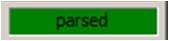
\includegraphics{parsed-icon.jpg}}}
 icon in the lower-right corner tells you
 that the spec has no parsing errors.}
will make the errors go away.

\pause
%
\noindent
%
When talking about the 
  \target{two-meanings-of-spec}%
  \ctindex{1}{specification!two meanings of}{spec-two-meanings}%
\emph{specification} of the one-bit clock, we
can mean one of two things:
\begin{itemize}
\item The complete module.  

\item The initial predicate and next-state relation.
\end{itemize}
It is usually clear from the context which is meant.  To avoid
confusion, we can talk about the module rather than the specification
when we mean the first.  We use the term
  \tindex{1}{behavior specification}%
  \ctindex{1}{specification!behavior}{spec-behavior}%
\emph{behavior specification} to mean the second.

  \tindex{1}{pretty printing}%
  \vspace{-\baselineskip}%
\btarget{pretty-printing}\subsection{The Pretty-Printed Version of Your Spec}

In addition to the \textsc{ascii} version of the module that you edit,
the Toolbox can display a ``pretty-printed'' version.  This requires
the 
  \ctindex{1}{pdflatex@\icmd{texttt}{pdflatex}}{pdflatex}%
\texttt{pdflatex} program to be installed on your computer.
Information on doing that and on configuring the Toolbox's
pretty-printing options can be found in 
\marginpar{\rref{help}{toolbox-help}{How to find help pages in
                                     the Toolbox.}}
\helppage{spec/pretty-printing}{the relevant Toolbox help page}.

To produce a pretty-printed version of the module, click on the
\textsf{File} menu and choose \textsf{Produce PDF Version}.  The 
pretty-printed version will be displayed in a separate window within
the Toolbox, with \tlaplus\ expressions shown approximately the way
they are printed in this hyperbook.  You can switch
 \marginpar{\popref{pretty-printing-bug}{Does it do something else?}}
between the \textsc{ascii} and
pretty-printed versions by clicking either the \textsf{TLA Module} or
\textsf{PDF Viewer} tab in the top-left corner of the module's window.
Editing the \textsc{ascii} version does not automatically change the
pretty-printed version.  You need to run the
\textsf{File}\,/\,\textsf{Produce PDF Version} command again to update it.

The pretty-printed version is produced in a file
\texttt{OneBitClock.pdf} that the Toolbox puts in the same directory
as the module file \texttt{OneBitClock.tla}.  You can print that file
to get a paper version.

\subsection{Checking the Specification}

Let's now get the 
  \tindex{1}{TLC}%
TLC model checker to check this specification.
\popref{create-new-model}{Create a new model}.  This opens a 
  \ctindex{1}{model!editor}{model-editor}% 
model editor on the model.  That editor has three pages; the model is
opened to the \textsf{Model Overview} page.

Enter $Init1$ and $Next1$ in the appropriate fields as the initial
predicate and next-state relation, and \popref{run-tlc}{run TLC}\@.
TLC runs for a couple of seconds and stops, reporting no errors.  This
means that the specification is sensible.  More precisely, it means
that our specification completely determines a collection of
behaviors.

\pause

\noindent
%
Let's change the specification so it doesn't determine a collection of
behaviors.  Go to the module editor (by clicking on its tab) and
modify the definition of $Next1$ by replacing \verb|/\ b' = 0| with
\verb|/\ b' = "xyz"|.  The second disjunct allows a step starting with
$b=0$ to set $b$ (change its value) to the
\rref{math}{strings}{string} \tlastring{xyz}.  Save the module, return
to the model editor, and run TLC again.  This time it reports the
error:
\begin{widedisplay}\small \tt
Attempted to check equality of string "xyz" with non-string: 0
\end{widedisplay}
The \textsf{TLC Errors} window also shows:%
 \marginpar{You can \popref{resize-errors-view}{resize the fields of the 
\textsf{TLC Errors} view}.}
\begin{display}
\scalebox{.75}{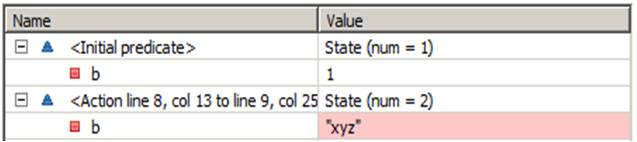
\includegraphics{OneBitClock-errortrace-1.jpg}}
\end{display}
This describes the following error trace: 
 \[ b=1 \s{.701} -> \s{.701} b = "xyz"
 \]
The trace is the beginning of a behavior that TLC was constructing
when it encountered an error.  The light-red background for the value
$"xyz"$ of $b$ indicates that it is different from the value of $b$ in
the previous state.  Double click on this line of the error trace:
\begin{display}
\scalebox{.75}{
\includegraphics{OneBitClock-errortrace-2.jpg}}
\end{display}
This raises the module editor, showing in part:
\begin{display}
\scalebox{.75}{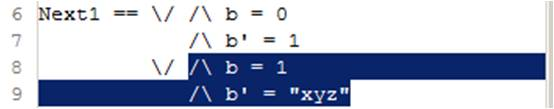
\includegraphics{OneBitClock-1.jpg}}
\end{display}
The highlighted portion is the disjunct of the next-state action $Next1$
that permits the step \,\tlabox{b=1 \, -> \, b = "xyz"}\,.

To calculate the possible next states from the state with $b="xyz"$,
TLC had to compute the value of the formula $"xyz"=0$.  (The rest of
the error message tells you that it was computing that formula in
order to evaluate the subformula $b=0$ of the definition of $Next1$.)
TLC couldn't do that because the semantics of \tlaplus\ do not
determine whether or not a string is equal to a 
  \marginpar{\popref{strings-vs-numbers}{Why shouldn't 
  \tlastring{xyz} be unequal
   to $0$?}}
number.  It could
therefore not determine if the formula $"xyz"=0$ equals \TRUE\ or
\FALSE, so it reported an error. 

Restore the original definition of $Next1$ by replacing $"xyz"$ with 0
and save the module.  Go back to the model editor and run TLC again.
It should once again find no error.

\pause
%
\noindent 
%
In the \textsf{Statistics} section of the \textsf{Model Checking
Results} page, the \textsf{State space progress} table tells you that
TLC found 2 distinct states.  The diameter of 1 means that 1 is the
largest number of steps (transitions from one state to the next) that
an execution of the one-bit clock can take before it repeats a state.

The one-bit clock is so simple there isn't much to check.  But there
is one property that we can and should check of just about any spec:
that it is 
  \tindex{1}{type correctness}%
``type correct''.  Type correctness of a \tlaplus\ specification
means that in every state of every behavior allowed by the spec, the
value of each variable is in the set of values that we expect it to
have.  For the one-bit clock, we expect the value of $b$ always to be
either 0 or 1.  This means that we expect the formula $b\in\{0,1\}$ to
be true in every state of every behavior of $b$.  If you are the least
bit unsure of what this formula means,
\target{sets}\textsf{\rref{math}{sets-intro}{detour to an introduction
to sets}}.\xlabel{main:simple-sets-return}

A formula that is true in all states of all behaviors allowed by a
spec is called an 
 \tindex{1}{invariant}%
\emph{invariant} of the spec.  Go to the
\textsf{Invariants} subsection of the \textsf{What to Check} section
of the model editor's\marginpar[.5]{Use the tabs at the top of the model
editor view to select the page.} \textsf{Model Overview} page.  Open
that subsection (by clicking on the {\bf \textsf{+}}), click on
\textsf{Add}, and enter the following formula:%
\begin{display}
\begin{twocols}
$b \in \{0, 1\}$
\midcol
\verb|b \in {0, 1}|
\end{twocols}
\end{display}
(Note that $\in$ is typed \verb|\in|.)  Click on \textsf{Finish}, and
then run TLC again on the model.  TLC should find no errors,
indicating that this formula is an invariant of the spec.

Because \tlaplus\ has no types, it has no type declarations.  As this
spec shows, there is no need for type declarations.  We don't need to
declare that $b$ is of type $\{0,1\}$ because that's implied by the
specification.  However, the reader of the spec doesn't discover that
until after she has read the definitions of the initial predicate and
next-state action.  In most real specifications, it's hard to
understand those definitions without knowing what the set of possible
values of each variable is.  It's a good idea to give the reader that
information by defining the 
 \ctindex{1}{invariant!type correctness}{inv-type-correct}%
 \ctindex{1}{type correctness!invariant}{type-correct-inv}%
type-correctness invariant in the spec,
right after the declaration of the variables.  So, let's add the
following definition to our spec, right after the declaration of $b$.
\begin{display}
\begin{twocols}
$TypeOK == b \in \{0,\,1\}$
\midcol
\verb|TypeOK == b \in {0,1}|
\end{twocols}
\end{display}
Save the spec and let's tidy up the model by using $TypeOK$ rather
than \tlabox{b \in \{0,\,1\}} as the invariant.  Go to the model
editor's \textsf{Model Overview} page, select the invariant you just
entered by clicking on it and hit \textsf{Edit} (or simply double-click on
the invariant), and replace the formula by \texttt{TypeOK}\@.  Click on
\textsf{Finish} and run TLC to check that you haven't made a mistake.

  \ctindex{1}{behavior!computing}{behavior-computing}%\
  \vspace{-\baselineskip}%
\subsection{Computing the Behaviors from the Specification}
\xlabel{sec:computing-clock-behaviors}

TLC checked that $TypeOK$ is an invariant of the specification of
the one-bit clock, meaning that it is true in all states of all
behaviors satisfying the specification.  TLC did this by computing
all possible behaviors that satisfy the initial predicate $Init1$ and
the next-state action $Next1$.  To understand how it does this, let's
see how we can do it.

We begin by computing one possible behavior.  A behavior is a sequence
of states.  To satisfy
the spec, the behavior's first state must satisfy the initial predicate
$Init1$.
A state is an assignment of values to all the spec's
variables, and this spec has only the single variable~$b$.  So to determine
a possible initial state, we must find an assignment of values to the
variable $b$ that satisfy $Init1$.  Since $Init1$ is defined to equal
 \[ (b=0) \/ (b=1) \]
there are obviously two such assignments: letting $b$ equal 0 or
letting it equal~1.  To construct one possible behavior satisfying the
spec, let's arbitrarily choose the starting state in which $b$
equals~1.  As before, we write that state as the formula $b=1$.

We next find a possible second state of the behavior.  For a behavior
to satisfy the spec, every pair of successive states must satisfy the
next-state action $Next1$, where the values of the unprimed variables
are the values assigned to them by the first state of the pair and the
values of the primed variables are the values assigned to them by the
second state of the pair.  The first state of our behavior is $b=1$.
To obtain the second state, we need to find a value for $b'$ that
satisfies $Next1$ when $b$ has the value 1.  We then let $b$ equal
that value in the second state.  To find this value, we substitute
$1$ for $b$ in $Next1$ and simplify the formula.  Recall that $Next1$
is defined to equal
 \[ \begin{disj}
    \begin{conj}
            b = 0 \\
            b' = 1
     \end{conj} \\
      \begin{conj}
         b = 1 \\
         b' = 0
     \end{conj}
    \end{disj}
 \]
We substitute 1 for $b$ and simplify as follows.
\begin{display}
\begin{tabbing}
   $\begin{disj}
    \begin{conj}
            1 = 0 \\
            b' = 1
     \end{conj} \\
      \begin{conj}
         1 = 1 \\
         b' = 0\vs{.75}
     \end{conj}
    \end{disj}$  \s{3} \=
    the formula obtained by substituting 1 for $b$ in $Next1$.\\
   $\mbox{} = \;\; \begin{disj}
    \begin{conj}
            \FALSE \\
            b' = 1
     \end{conj} \\
      \begin{conj}
         \TRUE \\
         b' = 0\vs{.75}
     \end{conj}
    \end{disj}$ \> because $\;(0=1) = \FALSE\;$ and $\;(1=1) = \TRUE$ \\
%
   $\mbox{} = \;\; \begin{disj}
         \FALSE    \\ b' = 0 
         \vs{.75}
    \end{disj}$ \> \begin{minipage}[t]{.75\textwidth}
                   because $\;\FALSE /\ F = \FALSE\;$ and 
                           $\;\TRUE /\ F = F\;$ \\
                   for any truth value $F$
                   \end{minipage} \\
%
   $\mbox{} = \;\; b'=0$ \> \begin{minipage}[t]{.6\textwidth}
                   because $\FALSE \/ F = F$ 
                   for any truth value $F$.
                   \end{minipage}
\end{tabbing}
\end{display}
This computation shows that if we substitute $1$ for $b$ in $Next1$,
then the only value we can then substitute for $b'$ that makes $Next1$
true is~0.  Hence, the second state of our behavior can only be $b=0$,
and our behavior starts with
 \[ b=1 \s{.701} -> \s{.701} b=0 \]
To find the third state of our behavior, we substitute $0$ for $b$ in
$Next1$ and find a value for $b'$ that makes $Next1$ true.  It should be
clear that the same type of calculation we just did shows that the only
possible value for $b'$ that makes $Next1$ true is~1.  (If it's not
clear, go ahead and do the calculation.)  The first three states
of our behavior therefore must be
 \[ b=1 \s{.701} -> \s{.701} b=0 \s{.701}-> \s{.701}  b=1
  \]
We could continue our calculations to find the fourth state of the
behavior, but we don't have to.  We've already seen that the only
possible state that can follow $b=1$ is $b=0$.  We can deduce
that \popref{finite-behaviors}{we must obtain the infinite behavior} 
 \[ b=1 \s{.701} -> \s{.701} b=0 \s{.701}-> \s{.701}  b=1 \s{.701} -> 
    \s{.701} b=0 \s{.701}-> \s{.701} \cdots
  \]
To find all possible behaviors, recall that the only other possible
starting state is $b=0$.  From the calculations we've already done,
we know that the only state that can follow $b=0$ is $b=1$.  We
therefore see that the only other possible behavior is
 \[ b=0 \s{.701}-> \s{.701}  b=1 \s{.701} -> \s{.701} b=0 \s{.701}-> \s{.701}  
    b=1 \s{.701} -> \s{.701} \cdots
  \]

\medskip

This example shows how we can compute all possible behaviors allowed
by a specification.  We construct as follows a
  \popref{directed-graph}{directed graph} 
$\mathcal{G}$, called the
  \ctindex{1}{graph!state}{graph-state}%
  \tindex{1}{state graph}%
  \target{main:state-graph}%
  \emph{state graph},
whose nodes are states:
\begin{enumerate}
\item We start by setting $\mathcal{G}$ to the set of all possible
initial states of behaviors, which we find by computing all possible
assignments of values to variables that make the initial predicate
true.

\item For every state $s$ in $\mathcal{G}$, we compute as follows all
possible states $t$ such that $s->t$ can be a step in a behavior.  We
substitute the values assigned to variables by $s$ for the unprimed
variables in the next-state action, and then compute all possible
assignments of values to the primed variables that make the next-state
action true.

\item For every state $t$ found in step 2: (i)~we add $t$ to $\mathcal{G}$
if it is not already in $\mathcal{G}$, and (ii)~we draw an edge from
$s$ to $t$.

\item We repeat steps 2 and 3 until no new states or edges can be
added to $\mathcal{G}$.
\end{enumerate}
If and when this process terminates, the nodes of $\mathcal{G}$
consist of all the 
  \tindex{1}{reachable state}%
  \ctindex{1}{state!reachable}{state-reachable}%
reachable states of the specifications---that is, all states that
occur in some behavior satisfying the specification.  Every behavior
satisfying the specification can be found by starting in an initial
state (found in step~1) and following a (possibly infinite) path in
$\mathcal{G}$.

\medskip

This procedure is used by TLC to compute all possible behaviors.  The
  \tindex{1}{state space progress table}%
\emph{State space progress} table in the \textsf{Statistics} section
of the \textsf{Model Checking Results} page gives the following
information about the graph $\mathcal{G}$ that it is constructing.
\begin{description}
\item[Diameter] The number of states in the longest path of
                $\mathcal{G}$ in which no state appears twice.
\item[States Found] The total number of (not necessarily distinct)
states it examined in step~1 or as successor states $t$ in step~2.

\item[Distinct States] The number of states that form the set of nodes
of $\mathcal{G}$.

\item[Queue Size] The number of states $s$ in $\mathcal{G}$ for which
step~2 has not yet been performed.
\end{description}
Of course, if the specification has an infinite number of reachable
states, this procedure will continue until $\mathcal{G}$ becomes so
large that TLC runs out of space.  However, this could take many years
because TLC keeps $\mathcal{G}$ and its queue of unexamined states on
disk when there is not enough room for them in memory.

Although TLC computes the behaviors that satisfy a specification the
same way we do, it's not nearly as smart as we are.  For example,
writing $1=b$ instead of $b=1$ in the initial predicate would make no
difference to us.  See how TLC reacts by making this change to the
definition of $Init1$ in module $OneBitClock$ and running TLC on the
model you created.  You will find that it produces the following error
report:
\begin{widedisplay} \tt
In evaluation, the identifier b is either undefined or not an operator.\\
{\darkaqua\underline{line 6, col 22 to line 6, col 22 of module OneBitClock}}.\\
The error occurred when TLC was evaluating the nested\\
expressions at the following positions:\\
0. {\darkaqua\underline{Line 6, column 22 to line 6, column 22 in OneBitClock}}
\end{widedisplay}
The underlined location indicators are links.  (They may not actually be
underlined in the Toolbox.)  Clicking on either of them jumps
to and highlights the $b$ in $1=b$.

TLC tries to find all possible initial states from the initial
predicate in a very simple-minded way.  It examines the predicate in a
linear fashion to try to find all possible assignments of values to
the variables.  When it encounters an occurrence of a variable $v$
whose value it has not yet determined, that occurrence must very
obviously determine the value of $v$.  This means that the occurrence
must be in a formula $v = e$ or $v\in e$ for some expression $e$ that
does not contain $v$.  For example, when TLC evaluated the initial
predicate
 \[ (b=0) \/ (1=b) \]
it first saw that it was a disjunction, so it examined the two
disjuncts separately.  The first disjunct, $b=0$, has the right form to
determine the value of $b$---that is, it has the form $v=e$ where $v$
is the variable $b$ and $e$ is the expression $0$.  However, when
examining the disjunct $1=b$, it first encountered the variable $b$ in
an expression that did not have the right form.  It therefore reported
that occurrence of $b$ as an error.  You can check that TLC has no
problem with the equivalent initial predicate
  \[ (b=0)\, \/ \, ((b=1) /\ (1=b))
  \]
because, when it encounters the expression $1=b$, it has already
determined the value of $b$.

\begin{aquestion}{tlc-answer-1}
What happens if you change the initial predicate to
 \[ (b=0)\, \/ \,((b=1) /\ (2=b))\]
and run TLC.
\end{aquestion}
%
These same remarks apply to the way TLC determines the possible
assignments to the primed variables from the next-state action when
performing step~2 of the procedure above.  The first time TLC
encounters a primed variable $v'$ whose value it has not yet
determined, that occurrence must be in a formula $v' = e$ or $v'\in e$
for some expression $e$ not containing $v'$.
 

\subsection{Other Ways of Writing the Behavior Specification}
\xlabel{main:one-bit:other-ways}

\rref{math}{otherops}{\textsf{If you are not intimately acquainted with the
propositional-logic operators $\Rightarrow$ (implication), $\equiv$
(equivalence), and $~$ (negation), detour here.}}\target{otherops}

\medskip

\noindent The astute reader will have noticed that the
two formulas $Init1$ and $TypeOK$, which equal $(b=0) \/ (b=1)$ and $b
\in \{0,\,1\}$, respectively, both assert that $b$ equals either 0 or
1.  In other words, these two formulas are equivalent---meaning that
the following formula equals $\TRUE$ for any value of $b$:
 \[ ((b=0) \/ (b=1)) \;\equiv\; (b \in \{0,\,1\})
 \]
%   \marginpar{\rref{math}{otherops}{Exactly what does 
%               \emph{equivalent} mean?}}  
The two formulas can be used interchangeably.
To test this, return to the Toolbox and select the \textsf{Model
Overview} page of the model editor.  Replace $Init1$ by $TypeOK$ in
the \textsf{Init} field and run TLC again.  You should find that
nothing has changed.

There are a number of different ways to write the next-state action.
This action should assert that $b'$ equals 1 if $b$ equals 0, and
equals 0 if $b$ equals 1.  Since the value of $b$ is equal to either 0
or 1 in every state of the behavior, an equivalent way to say this is
that $b'$ equals 1 if $b$ equals 0, else it equals 0.  This is expressed
by the formula $Next2$, that we define as follows.%
  \ctindex{1}{if then else@\icmd{textsc}{if}\icmd{ldots}\icmd{textsc}{then}\icmd{ldots}\icmd{textsc}{else}}{if-then-else}%
\begin{twocols}
$Next2  ==  b' = \IF b = 0 \THEN 1 \ELSE 0$
\midcol
\verb|Next2  ==  b' = IF b = 0 THEN 1 ELSE 0|
\end{twocols}
The meaning of the $\IF$\ldots$\THEN$\ldots$\ELSE\!\!\!$ construct
should be evident.

Unlike $Init1$ and $TypeOK$, the two formulas $Next1$ and $Next2$ are
not equivalent.  However, they are equivalent if $b$ equals 0 or 1.
More precisely, the following formula equals $\TRUE$ for
all values of $b$:
 \marginpar{\popref{main-impl-question}{\textsf{Why is this formula 
        true if $b$ equals 42?}}}
 \[ TypeOK \; => \; (Next1 \,\equiv\, Next2)
 \]
When used with $Init1$ as the initial predicate, both next-state
actions yield specifications for which each state of each behavior
satisfies $TypeOK$.  Hence, the truth of this formula implies that the
two specs are equivalent---meaning that they have the same set of
allowed behaviors.  Test this by copying and pasting the definition of
$Next2$ into the module (anywhere after the declaration of $b$),
saving the module, replacing $Next1$ by $Next2$ in the \textsf{Next}
field of the model, and running TLC again.

The method of writing the next-state action that I find most
elegant is to use the 
  \tindex{1}{modulus operator}% 
  \ctindex{1}{+5w@\mmath{\%} (modulus)}{+5w}%
  \rref{math}{math:modulus}{modulus operator $\%$},
where $a\,\%\, b$ is the remainder when $a$ is divided by $b$. 
Since $0\,\%\,2 = 0$, $1\,\%\,2 = 1$, and $2\,\%\,2 = 0$,
it's easy to check that, if $b$ equals 0 or 1, then $Next1$ and
$Next2$ are equivalent to the following formula.
\begin{display}
\begin{twocols}
$Next3  ==  b' = (b+1)\,\%\,2$
\midcol
\verb|Next3  ==  b' = (b + 1) % 2|
\end{twocols}
\end{display}
Add this definition to the module and save the module.  This will
generate a parsing error, informing you that the operator \,$\%$\, is
not defined.  The usual arithmetic operators, including $\,+\,$ and
$\,-\,$, are not built-in operators of \tlaplus.  Instead, they must be
imported from one of the \popref{standard-arith-modules}{standard
\protect\tlaplus\ arithmetic modules}, using an \textsc{extends} statement.
You will usually want to import the 
  \ctindex{1}{Integers module@\mmath{Integers} module}{integers-module}%
$Integers$ module, which you do
with the following statement:%
\begin{display}
\begin{twocols}
$\EXTENDS Integers$\ctindex{1}{extends@\icmd{textsc}{extends}}{extends}%
\midcol
\verb|EXTENDS Integers|
\end{twocols}
\end{display}
Add this statement to the 
beginning%
 \marginpar{\popref{extends-location}{Where can an \textsc{extends} go?}}
of the module and save the module.  Open the model editor's
\textsf{Model Overview} page, replace the next-state action $Next2$
with $Next3$, and run TLC to check this specification.

\pause

\noindent
Mathematics provides many different ways of expressing the same thing.
There are an infinite number of formulas equivalent to any given
formula.  For example, here's a formula that's equivalent to 
$Next2$.
\begin{display}
\begin{notla}
IF b = 0 THEN b' = 1
         ELSE b' = 0
\end{notla}
\begin{tlatex}
\@x{ {\IF} b \.{=} 0 \.{\THEN} b' \.{=} 1}%
\@x{\@s{35.71} \.{\ELSE} b' \.{=} 0}%
\end{tlatex}
\end{display}
As $Next1$ and $Next2$ show, even two next-state actions that are not
equivalent can yield equivalent specifications---that is,
specifications describing the same sets of behaviors.

\begin{aquestion}{logic-answer2}
Use the propositional operators $=>$ and $/\ $ to write a
next-state action that yields another equivalent
specification of the one-bit clock.
How many other next-state actions can you find that also
produce equivalent specifications?  
\end{aquestion}

\begin{aquestion}{logic-answer1}
Can inequivalent initial
predicates produce equivalent specifications?
\end{aquestion}
%
% \textsf{If you are not following the
% \emph{Principles} track and are uninterested in PlusCal, you can 
% \lref{section.\getrefnumber{sec:euclid}}{skip to Section~\ref{sec:euclid}.}}


% \subsection{Making the Spec Easier to Read and Rewrite}
% 
% \textbf{Not yet written.} Will discuss comments and the pretty-printed
% version, directing the reader to use Help if pretty-printing doesn't
% work in his Toolbox. 

% \bigskip

% \noindent
% \sref{proof}{theorems}{\textsf{To begin the Proof Track, click here.}}


\subsection{Specifying the Clock in PlusCal} \xlabel{sec:pcal-clock}

We now specify the 1-bit clock as a \lref{main:pluscal}{PlusCal} algorithm,
which means that we start learning the PlusCal language.  If at any
point you want to jump ahead, you can read the
   \hyperref{http://research.microsoft.com/en-us/um/people/lamport/tla/c-manual.pdf}{}{}{PlusCal
  language manual}.

In the Toolbox, \popref{open-new-spec}{open a new spec} and name the
specification and its root module \emph{PCalOneBitClock}.  The
algorithm is written inside a 
  \ctindex{1}{comment!multi-line}{comment-multi-line}%
  \tindex{1}{multi-line comment}%
multi-line comment, which is begun by
\verb|(*| and ended by \verb|*)|.  The easy way to create such a
comment is to put the 
  \popref{cursor}{cursor} at the left margin and type
\textsf{control+o} \textsf{control+s}.  (You can also right-click and
select \textsf{Start Boxed Comment}.)  Your file will now look about
like this.
\begin{verbatim}
-------------------------- MODULE PCalOneBitClock --------------------------

(***************************************************************************

 ***************************************************************************)
=============================================================================
\end{verbatim}
We need to choose an arbitrary name for the algorithm.  Let's call it
\emph{Clock}.  We start by typing this inside the
   comment:%
\begin{display}
\begin{twocols}
\verb|--|\textbf{algorithm} $Clock$ \{\\
\}
\midcol
\begin{verbatim}
--algorithm Clock {
}
\end{verbatim}
\end{twocols}
\end{display}
The 
  \ctindex{1}{algorithm token@\icmd{textbf}{-{}-algorithm} token}%
  {algorithm-token}%
\verb|--| in the token \verb|--|\textbf{algorithm} has no
significance; it's just a meaningless piece of required syntax that
you're otherwise unlikely to put in a comment.

The body of the algorithm appears between the curly braces \{\,\,\}.
It begins by declaring the variable $b$ and specifying its set of
possible initial values%
    \ctindex{1}{variable (PlusCal keyword)@\icmd{variable} (PlusCal keyword)}{variable-pcal}%
\begin{twocols}
\variable\ $b \in 
\{0, 1\}$;
\midcol
\verb|variable b \in {0, 1};|
\end{twocols}
Next comes the executed code, enclosed in curly braces.%
 \marginpar[-1.5]{ \popref{PCalOneBitClock}{\textsc{ascii} version 
  of the complete algorithm.}}
\begin{display}
\begin{tabbing}
\{ \pwhile\ (\TRUE) \= \{ \pif\ $(b = 0)$ $b := 1$ \pelse\ $b := 0$
\\
\> \}\\
\}
\end{tabbing}
\end{display}
You should be able to figure out the meaning of this PlusCal code
because it looks very much like code written in C or a language like
Java that uses C's syntax.  The major difference is that in PlusCal,
  \marginpar{\popref{c-syntax}{Why doesn't PlusCal use \texttt{=}
for assignment?}}%
the equality relation is written \,\verb|=|\, instead of
\,\verb|==|\,, and assignment is written \,\verb|:=|\, instead of
\,\verb|=|\,.  (You can make it look more like C by adding 
semi-colons after the two assignments.)

% We next have to tell the translator 
%   \ctindex{1}{PlusCal translation!placement of}{pluscal-trans-placement}%
% where to put the \tlaplus\ translation.  It's best to put it right
% after the comment containing the PlusCal code.  You do this by placing
% the following two lines there.
%     \ctindex{1}{comment!end-of-line}{comment-end-of-line}%
%   \ctindex{1}{+2oj@\mmath{\icmd{backslash}*} (end-of-line comment)}{+2oj}%
%   \tindex{1}{end-of-line comment}%
% (A \verb|\*| begins a comment that ends at the end of the
% line.)
%   \ctindex{1}{begin translation@\icmd{texttt}{begin translation}}%
%   {begin-translation}%
%   \ctindex{1}{end translation@\icmd{texttt}{end translation}}%
%   {end-translation}%
% \begin{display}
% \begin{verbatim}
% \* BEGIN TRANSLATION
% \* END TRANSLATION
% \end{verbatim}
% \end{display}
%
Save the module.  Now 
  \ctindex{1}{PlusCal!translator}{pluscal-translator}%
call the translator by selecting the \textsf{File} menu's
\textsf{Translate PlusCal Algorithm} option or by typing
\textsf{control+t}.  The translator will insert the algorithm's
\tlaplus\ translation after the end of the comment containing the
algorithm, between the two comment lines:
\begin{display}
\verb|\* BEGIN TRANSLATION|  
 \ctindex{1}{begin translation@\icmd{texttt}{BEGIN TRANSLATION}}%
  {begin-translation}%
  \ctindex{1}{end translation@\icmd{texttt}{END TRANSLATION}}%
  {end-translation}%
\s{1}and\s{1}\verb|\* END TRANSLATION|
\end{display}
If the file already contains these two comment lines, the translation
will be put between them, replacing anything that's already there.

The important parts of the translation are the declaration
of the variable $b$ and the definitions of the initial predicate
$Init$ and the next-state action $Next$.  Those two definitions are
the following
\begin{display}
\begin{notla}
Init == b \in {0, 1}

Next == IF b = 0 THEN  b' = 1
                 ELSE  b' = 0
\end{notla}
\begin{tlatex}
\@x{ Init\@s{4.12} \.{\defeq} b \.{\in} \{ 0 ,\, 1 \}}%
\par\vspace{8.0pt}%
\@x{ Next \.{\defeq} {\IF} b \.{=} 0 \.{\THEN}\@s{4.1} b' \.{=} 1}%
\@x{\@s{75.55} \.{\ELSE}\@s{4.1} b' \.{=} 0}%
\end{tlatex}
\end{display}
except that the translator formats them differently, inserting a
comment and some unnecessary $/\ $ operators at the beginning of
formulas.  (A bulleted list of conjuncts can consist of just one
conjunct.)

We have seen above that this definition of $Init$ is equivalent to the
definition of $Init1$ in module $OneBitClock$.  We have seen the
definition of $Next$ above too, where we observed that it is
equivalent to the definition of $Next2$ in the $OneBitClock$ module.

The translation also produces definitions of the symbols $var$ and $Spec$.
You should ignore them for now.

\bigskip

As you have probably guessed, if we replace the \pif\,/\,\pelse\
statement in the PlusCal code with the statement $b := (b+1)\,\%\,2$, the
translation will define $Next$ to be the formula $Next3$ we defined
above.  Try it.  As before, the Toolbox will complain that \,$\%$\, is
undefined.  You have to add an $\EXTENDS Integers$ statement to the
beginning of the module.
%try

% 1st
%%%%%%%%%%%%%%%
\begin{en}
\newpage
   \tindex{1}{Die Hard}%
\vspace{-\baselineskip}%

\section{The Die Hard Problem} \xlabel{sec:diehard}

In the movie \emph{Die Hard 3}, the heroes must solve the problem of
obtaining exactly 4 gallons of water using a 5 gallon jug, a 3 gallon
jug, and a water faucet.  We now apply \tlaplus\ and the TLC
model checker to solve this problem.
\end{en}

\begin{ch}
\newpage
   \tindex{1}{Die Hard}%
\vspace{-\baselineskip}%

\section{Die Hard 问题} \xlabel{sec:diehard}

在电影《虎胆龙威(三)》中,
两位英雄必须解决这样一个问题:
用一个 5 加仑的水壶,一个 3 加仑的水壶,\fixme{和一个水龙头},
如何得到 4 加仑的水?
现在,我们用 \tlaplus\ 和 \tlc{} 模型验证器解决该问题。
\end{ch}
%%%%%%%%%%%%%%%

% 2nd
%%%%%%%%%%%%%%%
\begin{en}
\subsection{Representing the Problem in TLAPlus}%

The first step in solving the problem is to model the physical system
of heroes, jugs, and faucet mathematically as a discrete system.
%
The only relevant state of the hero/jug/faucet system is the amount of
water in the two jugs.  So, we model the system with two variables,
$big$ and $small$, whose values represent the number of gallons of
water in the two jugs.  After choosing the variables, a good way to
figure out how to write a specification is to write down the first few
states of a possible behavior of the system.  Initially, the jugs are
empty, so $big$ and $small$ both equal~0.  Here's one possible
beginning of a behavior.  (Remember that a state is an assignment of
values to the variables, in this case $big$ and $small$.)
\begin{display}
\begin{tabbing}
The small jug is filled from the big one: \= \kill
%
\>
$\dhstate{0}{0}$\V{1.01}
%
\>The big jug is filled from the faucet.\'\s{2.7}$\downarrow$\V{.31}
%
\>
$\dhstate{5}{0}$\V{1.01} 
%
%
\>The small jug is filled from the big one.\'\s{2.7}$\downarrow$\V{.31}
%
\>
$\dhstate{2}{3}$\V{1.01}
%
\>The small jug is emptied (onto the ground).\'\s{2.7}$\downarrow$\V{.31}
%
\> $\dhstate{2}{0}$
\end{tabbing}
\end{display}
\end{en}

\begin{ch}
  \subsection{用 TLAPlus 描述 Die Hard 问题}%

  解决该问题的首要任务
  是以数学的方式将由英雄、水壶和水龙头构成的物理系统建模为一个离散系统。
  在该物理系统中,唯一相关的状态是两个水壶中的水量。
  因此,我们用两个变量建模该系统:
  $big$ 和 $small$ 分别表示大小两个水壶中的水量。
  选定变量之后,弄清如何编写规约的一个好方法是
  先写系统的某个行为的头几个状态。
  一开始,水壶是空的,因此 $big$ 和 $small$ 都等于 0。
  系统的某个行为的开头可能如下所示
  (一个状态是一种变量赋值。
  在本例中,变量是 $big$ 和 $small$。):
  \begin{display}
  \begin{tabbing}
  将大水壶里的水倒入小水壶,直到小水壶装满水为止。\= \kill
  %
  \>
  $\dhstate{0}{0}$\V{1.01}
  %
  \>大水壶从水龙头灌满水。\'\s{2.7}$\downarrow$\V{.31}
  %
  \>
  $\dhstate{5}{0}$\V{1.01} 
  %
  %
  \>将大水壶里的水倒入小水壶,直到小水壶装满水为止。\'\s{2.7}$\downarrow$\V{.31}
  %
  \>
  $\dhstate{2}{3}$\V{1.01}
  %
  \>将小水壶中的水倾空(倒在地上)。\'\s{2.7}$\downarrow$\V{.31}
  %
  \> $\dhstate{2}{0}$
  \end{tabbing}
  \end{display}
\end{ch}
%%%%%%%%%%%%%%%
%  in the same paragraph
% 3rd
%%%%%%%%%%%%%%%
\begin{en}
A little thought reveals that there are three kinds of steps in a
behavior:
\begin{itemize}
\item Filling a jug.
\item Emptying a jug.
\item Pouring from one jug to the other.  There are two cases:
\begin{itemize}
\item This empties the first jug.
\item This fills the second jug, possibly leaving water
      in the first jug.
\end{itemize}
\end{itemize}
We can now write the specification.  Let's \popref{open-new-spec}{open
a new specification} named $DieHard$ in the Toolbox.  Since the spec
will require arithmetic operations, it begins with:
\begin{display}
\begin{twocols}%[.45]
$\EXTENDS\ Integers$
\midcol
\verb|EXTENDS Integers|
\end{twocols}
\end{display}
We declare the variables and write the initial predicate, which we
give the conventional name $Init$.
\smallskip
\begin{display}
\begin{twocols}%[.45]
$\VARIABLES big,\ small$ \V{.4}
$Init == 
\begin{conj}
big = 0 \\ small = 0
\end{conj}
$
\midcol
\verb*|VARIABLES big, small|\V{.4}
\verb*|Init == /\ big = 0| \\
\verb*|        /\ small = 0|
\end{twocols}
\end{display}
\smallskip
\end{en}
% in the same paragraph 
\begin{ch}
  稍作思考,我们会发现一个行为包含三类\tlastep{}:
  \begin{itemize}
  \item (从水龙头)装满某个水壶。
  \item 倾空某个水壶。
  \item 从一个水壶往另一个水壶倒水。这分两种情况:
  \begin{itemize}
  \item 第一个水壶被倾空。
  \item 第二个水壶被装满。此时,第一个水壶中可能还有水。
  \end{itemize}
  \end{itemize}
  现在,我们可以编写规约了。
  在\tlatoolbox{}中\popref{open-new-spec}{打开一个新的规约},
  命名为 $DieHard$。
  由于该规约需要用到算术操作,所以它以
  \begin{display}
  \begin{twocols}%[.45]
  $\EXTENDS\ Integers$
  \midcol
  \verb|EXTENDS Integers|
  \end{twocols}
  \end{display}
  开头。
  我们声明变量,编写\tlainitpredicate{},
  \fixme{并按照惯例}将\tlainitpredicate{}命名为 $Init$。
  \smallskip
  \begin{display}
  \begin{twocols}%[.45]
  $\VARIABLES big,\ small$ \V{.4}
  $Init == 
  \begin{conj}
  big = 0 \\ small = 0
  \end{conj}
  $
  \midcol
  \verb*|VARIABLES big, small|\V{.4}
  \verb*|Init == /\ big = 0| \\
  \verb*|        /\ small = 0|
  \end{twocols}
  \end{display}
  \smallskip
\end{ch}
%%%%%%%%%%%%%%%
% % in the same paragraph
% 4th
%%%%%%%%%%%%%%%
\begin{en}
Each of the three possible kinds of steps has two possibilities---one
for each jug (each first jug for the third type).  This suggests
writing the next state action as the disjunction of six formulas, each
allowing one of these six possible kinds of step.  We can therefore
define the next-state action, which by convention is called $Next$, as
follows:
\medskip
\begin{twocols}%[.45]
\begin{notla}
Next == \/ FillSmall 
        \/ FillBig    
        \/ EmptySmall 
        \/ EmptyBig    
        \/ SmallToBig    
        \/ BigToSmall 
\end{notla}
\begin{tlatex}
\@x{ Next \.{\defeq} \.{\lor} FillSmall}%
\@x{\@s{39.83} \.{\lor} FillBig}%
\@x{\@s{39.83} \.{\lor} EmptySmall}%
\@x{\@s{39.83} \.{\lor} EmptyBig}%
\@x{\@s{39.83} \.{\lor} SmallToBig}%
\@x{\@s{39.83} \.{\lor} BigToSmall}%
\end{tlatex}
\midcol
\begin{verbatim*}
Next == \/ FillSmall 
        \/ FillBig    
        \/ EmptySmall 
        \/ EmptyBig    
        \/ SmallToBig    
        \/ BigToSmall 
\end{verbatim*}
\end{twocols}
\medskip
\end{en}
% in the same paragraph 
\begin{ch}
  每一类可能的\tlastep{}都有两种情况,
  分别对应于不同的水壶
  (对于第三类\tlastep{},第一个水壶可以是两个水壶中的任意一个)。
  这提示我们将\tlanextstateaction{}写成 6 个公式的析取式,
  每个公式对应一类可能的\tlastep{}。
  因此,我们如下定义\tlanextstateaction{},并按照惯例将其命名为 $Next$:
  \medskip
  \begin{twocols}%[.45]
  \begin{notla}
  Next == \/ FillSmall 
	  \/ FillBig    
	  \/ EmptySmall 
	  \/ EmptyBig    
	  \/ SmallToBig    
	  \/ BigToSmall 
  \end{notla}
  \begin{tlatex}
  \@x{ Next \.{\defeq} \.{\lor} FillSmall}%
  \@x{\@s{39.83} \.{\lor} FillBig}%
  \@x{\@s{39.83} \.{\lor} EmptySmall}%
  \@x{\@s{39.83} \.{\lor} EmptyBig}%
  \@x{\@s{39.83} \.{\lor} SmallToBig}%
  \@x{\@s{39.83} \.{\lor} BigToSmall}%
  \end{tlatex}
  \midcol
  \begin{verbatim*}
  Next == \/ FillSmall 
	  \/ FillBig    
	  \/ EmptySmall 
	  \/ EmptyBig    
	  \/ SmallToBig    
	  \/ BigToSmall 
  \end{verbatim*}
  \end{twocols}
  \medskip
\end{ch}
%%%%%%%%%%%%%%%
% % in the same paragraph
% 5th
%%%%%%%%%%%%%%%
\begin{en}
The definitions of the six formulas $FillSmall$, \ldots\,, $BigToSmall$,
which often called 
 \tindex{1}{subaction}%
\emph{subactions} of the next-state action, must
precede the definition of $Next$ in the module.  (In \tlaplus, a
symbol must be defined or declared before it can be used.)  Let's now
define them.  
\end{en}
% in the same paragraph 
\begin{ch}
  这 6 个公式 —— 通常称为\tlanextstateaction{}的%
   \tindex{1}{subaction}%
  \emph{\tlasubaction{}} —— 
  的定义必须出现在 $Next$ 的定义之前。
  (在 \tlaplus 中,一个符号需要先定义或者先声明之后才可使用。)
  现在,我们定义这些\tlasubaction{}。
\end{ch}
%%%%%%%%%%%%%%%

% 6th
%%%%%%%%%%%%%%%
\begin{en}
Most programmers would expect the definition of $FillSmall$ to be
 \[ FillSmall == small' = 3 \]
This formula is certainly satisfied by a step like
 \[ \dhstate{2}{1} -> \dhstate{2}{3}
 \]
However, the formula is also satisfied by this step
  \[ \dhstate{2}{1} -> \dhstate{\sqrt{42}}{3}
 \]
because substituting
 \[ big <- 2, \ \ small <- 1, \ \ big' <- \sqrt{42}, \ \ small' <- 3
 \]
in the formula produces the true formula $3=3$.  
\end{en}

\begin{ch}
  大多数程序员期望看到如下定义的 $FillSmall$ 公式:
  \[ FillSmall == small' = 3 \]
  该公式当然可以被如下所示的\tlastep{}所满足:
  \[ \dhstate{2}{1} -> \dhstate{2}{3}
  \]
  但是,它也可以被\tlastep{}
  \[ \dhstate{2}{1} -> \dhstate{\sqrt{42}}{3}
  \]
  所满足,这是因为在公式中施行替换
  \[ big <- 2, \ \ small <- 1, \ \ big' <- \sqrt{42}, \ \ small' <- 3
  \]
  会产生永真式 $3=3$。
\end{ch}
%%%%%%%%%%%%%%%
%  % in the same paragraph
% 7th
%%%%%%%%%%%%%%%
\begin{en}
Since a step that
fills the small jug should leave the contents of the big jug
unchanged, the subaction $FillSmall$ must assert that $big'$ equals
$big$.  With this observation, the definitions of the first four
subactions are obvious:
 \medskip
\begin{twocols}%[.45]
\begin{notla}
FillSmall  == /\ small' = 3 
              /\ big' = big

FillBig    == /\ big' = 5 
              /\ small' = small

EmptySmall == /\ small' = 0 
              /\ big' = big

EmptyBig   == /\ big' = 0 
              /\ small' = small
\end{notla}
\begin{tlatex}
\@x{ FillSmall\@s{13.03} \.{\defeq} \.{\land} small' \.{=} 3}%
\@x{\@s{72.70} \.{\land} big' \.{=} big}%
\@pvspace{8.0pt}%
\@x{ FillBig\@s{23.00} \.{\defeq} \.{\land} big' \.{=} 5}%
\@x{\@s{72.70} \.{\land} small' \.{=} small}%
\@pvspace{8.0pt}%
\@x{ EmptySmall \.{\defeq} \.{\land} small' \.{=} 0}%
\@x{\@s{72.70} \.{\land} big' \.{=} big}%
\@pvspace{8.0pt}%
\@x{ EmptyBig\@s{9.97} \.{\defeq} \.{\land} big' \.{=} 0}%
\@x{\@s{72.70} \.{\land} small' \.{=} small}%
\end{tlatex}
\midcol
\begin{verbatim*}
FillSmall  == /\ small' = 3 
              /\ big' = big

FillBig    == /\ big' = 5 
              /\ small' = small

EmptySmall == /\ small' = 0 
              /\ big' = big

EmptyBig   == /\ big' = 0 
              /\ small' = small
\end{verbatim*} 
\end{twocols} 
\medskip
\end{en}
% in the same paragraph 
\begin{ch}
  由于``将小水壶装满''这一\tlastep{}应该保持大水壶里的水量不变,
  所以\tlasubaction{} $FillSmall$ 必须保证 $big'$ 等于 $big$。
  \fixme{基于这种观察},
  前四个\tlasubaction{}的定义是显而易见的:
  \medskip
  \begin{twocols}%[.45]
  \begin{notla}
  FillSmall  == /\ small' = 3 
		/\ big' = big

  FillBig    == /\ big' = 5 
		/\ small' = small

  EmptySmall == /\ small' = 0 
		/\ big' = big

  EmptyBig   == /\ big' = 0 
		/\ small' = small
  \end{notla}
  \begin{tlatex}
  \@x{ FillSmall\@s{13.03} \.{\defeq} \.{\land} small' \.{=} 3}%
  \@x{\@s{72.70} \.{\land} big' \.{=} big}%
  \@pvspace{8.0pt}%
  \@x{ FillBig\@s{23.00} \.{\defeq} \.{\land} big' \.{=} 5}%
  \@x{\@s{72.70} \.{\land} small' \.{=} small}%
  \@pvspace{8.0pt}%
  \@x{ EmptySmall \.{\defeq} \.{\land} small' \.{=} 0}%
  \@x{\@s{72.70} \.{\land} big' \.{=} big}%
  \@pvspace{8.0pt}%
  \@x{ EmptyBig\@s{9.97} \.{\defeq} \.{\land} big' \.{=} 0}%
  \@x{\@s{72.70} \.{\land} small' \.{=} small}%
  \end{tlatex}
  \midcol
  \begin{verbatim*}
  FillSmall  == /\ small' = 3 
		/\ big' = big

  FillBig    == /\ big' = 5 
		/\ small' = small

  EmptySmall == /\ small' = 0 
		/\ big' = big

  EmptyBig   == /\ big' = 0 
		/\ small' = small
  \end{verbatim*} 
  \end{twocols} 
  \medskip
\end{ch}
%%%%%%%%%%%%%%%
% % in the same paragraph
% 8th
%%%%%%%%%%%%%%%
\begin{en}
The definitions of the last two, $SmallToBig$ and $BigToSmall$, are
trickier because each has two cases.  Let's consider $SmallToBig$.
We can express the two possibilities as the disjunction of two
formulas:
\begin{display}
\begin{notla}
SmallToBig == \/ /\ big + small > 5
                 /\ big' = 5
                 /\ small' = small - (5 - big)
              \/ /\ big + small =< 5
                 /\ big' = big + small
                 /\ small' = 0
\end{notla}
\begin{tlatex}
\@x{ SmallToBig \.{\defeq} \.{\lor} \.{\land} big \.{+} small \.{>} 5}%
\@x{\@s{81.62} \.{\land} big' \.{=} 5}%
\@x{\@s{81.62} \.{\land} small' \.{=} small \.{-} ( 5 \.{-} big )}%
%
\marginpar{If the water doesn't all fit in the big jug, then $5-big$
           gallons are poured out of the little jug.} 
%
\@x{\@s{70.51} \.{\lor} \.{\land} big \.{+} small \.{\leq} 5}%
\@x{\@s{81.62} \.{\land} big' \.{=} big \.{+} small}%
\@x{\@s{81.62} \.{\land} small' \.{=} 0}%
\end{tlatex}
\end{display}
\end{en}
% in the same paragraph 
\begin{ch}
  后两个\tlasubaction{} $SmalltoBig$ 和 $BigToSmall$ 的定义稍显复杂,
  因为每个都有两种情况。
  考虑 $SmallToBig$。
  我们可以将它的两种情况表示成两个公式的析取:
  \begin{display}
  \begin{notla}
  SmallToBig == \/ /\ big + small > 5
		   /\ big' = 5
		   /\ small' = small - (5 - big)
		\/ /\ big + small =< 5
		   /\ big' = big + small
		   /\ small' = 0
  \end{notla}
  \begin{tlatex}
  \@x{ SmallToBig \.{\defeq} \.{\lor} \.{\land} big \.{+} small \.{>} 5}%
  \@x{\@s{81.62} \.{\land} big' \.{=} 5}%
  \@x{\@s{81.62} \.{\land} small' \.{=} small \.{-} ( 5 \.{-} big )}%
  %
  \marginpar{如果大水壶装不下小水壶中所有的水,
    那么从小水壶中倒入大水壶中的水量是 $5-big$ 加仑。} 
  %
  \@x{\@s{70.51} \.{\lor} \.{\land} big \.{+} small \.{\leq} 5}%
  \@x{\@s{81.62} \.{\land} big' \.{=} big \.{+} small}%
  \@x{\@s{81.62} \.{\land} small' \.{=} 0}%
  \end{tlatex}
  \end{display}
\end{ch}
%%%%%%%%%%%%%%%
% % in the same paragraph
% 9th
%%%%%%%%%%%%%%%
\begin{en}
This definition is fine, but it can be expressed more compactly.
Observe that a $SmallToBig$ step sets the value of $big$ to the
smaller of $big+small$ and 5.  Let's define $Min$ so that $Min(m, n)$
is the smaller of $m$ and $n$, if $m$ and $n$ are numbers.
\begin{twocols}
\begin{notla}
Min(m,n) == IF m < n THEN m ELSE n
\end{notla}
\begin{tlatex}
\@x{ Min ( m ,\, n ) \.{\defeq} {\IF} m \.{<} n \.{\THEN} m \.{\ELSE} n}%
\end{tlatex}
\midcol
\verb|Min(m,n) == IF m < n THEN m ELSE n|
\end{twocols}
Since the amount of water removed from the small jug equals the amount
added to the big jug, we can define $SmallToBig$ by:
\begin{display}
\begin{notla}
SmallToBig == /\ big' = Min(big + small, 5)
              /\ small' = small - (big' - big)
\end{notla}
\begin{tlatex}
 \@x{ SmallToBig \.{\defeq} \.{\land} big' \.{=} Min ( big \.{+} small
 ,\, 5 )}%
 \@x{\@s{70.51} \.{\land} small' \.{=} small\@s{0.54} \.{-} ( big'
 \.{-} big )}%
\end{tlatex}
\end{display}
\end{en}
% in the same paragraph 
\begin{ch}
  这个定义还不错,但是可以表达得更紧凑些。
  注意到 $SmallToBig$ \tlastep{} 将 $big$ 设置为 $big+small$ 与 5 中的较小值。
  我们定义 $Min$, 使得 $Min(m,n)$ 等于 $m$ 与 $n$ 的较小值
  (如果 $m$ 与 $n$ 是数字)。
  \begin{twocols}
  \begin{notla}
  Min(m,n) == IF m < n THEN m ELSE n
  \end{notla}
  \begin{tlatex}
  \@x{ Min ( m ,\, n ) \.{\defeq} {\IF} m \.{<} n \.{\THEN} m \.{\ELSE} n}%
  \end{tlatex}
  \midcol
  \verb|Min(m,n) == IF m < n THEN m ELSE n|
  \end{twocols}
  因为从小水壶中倒出的水量等于大水壶增加的水量,
  所以我们可以如下定义 $SmallToBig$:
  \begin{display}
  \begin{notla}
  SmallToBig == /\ big' = Min(big + small, 5)
		/\ small' = small - (big' - big)
  \end{notla}
  \begin{tlatex}
   \@x{ SmallToBig \.{\defeq} \.{\land} big' \.{=} Min ( big \.{+} small
   ,\, 5 )}%
   \@x{\@s{70.51} \.{\land} small' \.{=} small\@s{0.54} \.{-} ( big'
   \.{-} big )}%
  \end{tlatex}
  \end{display}
\end{ch}
%%%%%%%%%%%%%%%
% % in the same paragraph
% 10th
%%%%%%%%%%%%%%%
\begin{en}
This definition has one drawback.  When reading an action formula, we
often want to see how a particular variable's value changes.  This is
easiest to do if the value of the primed variable is expressed as a
function of the values of the unprimed variables.  However, this
definition expresses the value of $small'$ in terms of $big'$ as well
as of $big$ and $small$.  We could fix that by writing the definition as:
\begin{display}
\begin{notla}
SmallToBig == /\ big' = Min(big + small, 5)
              /\ small' = small - (Min(big + small, 5) - big)
\end{notla}
\begin{tlatex}
 \@x{ SmallToBig \.{\defeq} \.{\land} big' \.{=} Min ( big \.{+} small
 ,\, 5 )}%
 \@x{\@s{70.51} \.{\land} small' \.{=} small\@s{0.54} \.{-} ( Min ( big
 \.{+} small ,\, 5 ) \.{-} big )}%
\end{tlatex}
\end{display}
\end{en}
% in the same paragraph 
\begin{ch}
  这个定义有一个缺陷。
  当阅读一个\tlaaction{}公式时,
  我们通常想知道一个特定变量的值是如何变化的。
  如果\tlaprimedvariable{}的值被表示成\tlaunprimedvariable{}的值的函数,
  那么这\fixme{很容易}做到。
  但是,该定义用 $big'$(以及 $big$ 与 $small$)的值来表示 $small'$ 的值。
  我们可以通过重写定义修复这个缺陷:
  \begin{display}
  \begin{notla}
  SmallToBig == /\ big' = Min(big + small, 5)
		/\ small' = small - (Min(big + small, 5) - big)
  \end{notla}
  \begin{tlatex}
   \@x{ SmallToBig \.{\defeq} \.{\land} big' \.{=} Min ( big \.{+} small
   ,\, 5 )}%
   \@x{\@s{70.51} \.{\land} small' \.{=} small\@s{0.54} \.{-} ( Min ( big
   \.{+} small ,\, 5 ) \.{-} big )}%
  \end{tlatex}
  \end{display}
\end{ch}
%%%%%%%%%%%%%%%
% % in the same paragraph
% 11th
%%%%%%%%%%%%%%%
\begin{en}
However, it's better not to repeat the expression $Min(big + small, 5)$.
I find it more elegant to write the action in terms the amount
of water poured from one jug to the other.  I prefer writing the
action as follows, using the \tlaplus\ 
  \rref{math}{let-in}{\textsc{let}\,/\,\textsc{in} construct},
which allows us to make local definitions within an expression.
 \medskip
\begin{twocols}%[.45]
\setboolean{shading}{true}
\begin{notla}
SmallToBig == 
  LET poured == Min(big + small, 5) - big
  IN  /\ big'   = big + poured
      /\ small' = small - poured
\end{notla}
\begin{tlatex}
\@x{ SmallToBig \.{\defeq}}%
 \@x{\@s{8.2} \.{\LET} poured \.{\defeq} Min ( big \.{+} small ,\, 5 ) \.{-}
 big}%
\@x{\@s{8.2} \.{\IN} \.{\land} big'\@s{10.88} \.{=} big \.{+} poured}%
\@x{\@s{28.59} \.{\land} small' \.{=} small \.{-} poured}%
\end{tlatex}
\midcol
\begin{verbatim*}
SmallToBig == 
  LET poured == Min(big + small, 5) - big
  IN  /\ big'   = big + poured
      /\ small' = small - poured
\end{verbatim*}
\end{twocols}
 \medskip
(Note that $poured$ equals $Min(small, 5-big)$.)
\end{en}
% in the same paragraph
\begin{ch}
  不过,最好不要重复表达式 $Min(big + small, 5)$。
  我发现使用\fixme{从一个水壶到另一个水壶的倒水量}来表达该\tlaaction{}更为简练。
  我更喜欢使用 \tlaplus\ 提供的
    \rref{math}{let-in}{\textsc{let}\,/\,\textsc{in} \tlaconstruct{}}
  将它写成如下形式(\textsc{let}\,/\,\textsc{in} 允许我们\fixme{在表达式内部给出局部定义}):
  \medskip
  \begin{twocols}%[.45]
  \setboolean{shading}{true}
  \begin{notla}
  SmallToBig == 
    LET poured == Min(big + small, 5) - big
    IN  /\ big'   = big + poured
	/\ small' = small - poured
  \end{notla}
  \begin{tlatex}
  \@x{ SmallToBig \.{\defeq}}%
   \@x{\@s{8.2} \.{\LET} poured \.{\defeq} Min ( big \.{+} small ,\, 5 ) \.{-}
   big}%
  \@x{\@s{8.2} \.{\IN} \.{\land} big'\@s{10.88} \.{=} big \.{+} poured}%
  \@x{\@s{28.59} \.{\land} small' \.{=} small \.{-} poured}%
  \end{tlatex}
  \midcol
  \begin{verbatim*}
  SmallToBig == 
    LET poured == Min(big + small, 5) - big
    IN  /\ big'   = big + poured
	/\ small' = small - poured
  \end{verbatim*}
  \end{twocols}
   \medskip
  (注意 $poured$ 等于 $Min(small, 5-big)$。)
\end{ch}
%%%%%%%%%%%%%%%
% in the same paragraph
% 12th
%%%%%%%%%%%%%%%
\begin{en}
The definition of the $BigToSmall$ subaction is similar.
 \medskip
\begin{twocols}
\begin{notla}
BigToSmall == 
  LET poured == Min(big + small, 3) - small
  IN  /\ big'   = big - poured
      /\ small' = small + poured
\end{notla}
\begin{tlatex}
\@x{ BigToSmall \.{\defeq}}%
 \@x{\@s{8.2} \.{\LET} poured \.{\defeq} Min ( big \.{+} small ,\, 3 ) \.{-}
 small}%
\@x{\@s{8.2} \.{\IN} \.{\land} big' \@s{10.88} \.{=} big \.{-} poured}%
\@x{\@s{28.59} \.{\land} small' \.{=} small \.{+} poured}%
\end{tlatex}
\midcol
\begin{verbatim*}
BigToSmall == 
  LET poured == Min(big + small, 3) - small
  IN  /\ big'   = big - poured
      /\ small' = small + poured
\end{verbatim*}
\end{twocols}
 \medskip
\end{en}
% in the same paragraph
\begin{ch}
  \tlasubaction{} $BigToSmall$ 的定义与之类似。
 \medskip
  \begin{twocols}
  \begin{notla}
  BigToSmall == 
    LET poured == Min(big + small, 3) - small
    IN  /\ big'   = big - poured
	/\ small' = small + poured
  \end{notla}
  \begin{tlatex}
  \@x{ BigToSmall \.{\defeq}}%
   \@x{\@s{8.2} \.{\LET} poured \.{\defeq} Min ( big \.{+} small ,\, 3 ) \.{-}
   small}%
  \@x{\@s{8.2} \.{\IN} \.{\land} big' \@s{10.88} \.{=} big \.{-} poured}%
  \@x{\@s{28.59} \.{\land} small' \.{=} small \.{+} poured}%
  \end{tlatex}
  \midcol
  \begin{verbatim*}
  BigToSmall == 
    LET poured == Min(big + small, 3) - small
    IN  /\ big'   = big - poured
	/\ small' = small + poured
  \end{verbatim*}
  \end{twocols}
 \medskip
\end{ch}
%%%%%%%%%%%%%%%
% in the same paragraph
% 13th
%%%%%%%%%%%%%%%
We should also define a type invariant.  Clearly, the values of
both $big$ and $small$ should be natural numbers, with $big\leq 5$
and $small\leq3$.  To express this, we use the operator 
  \ctindex{1}{+3i@\mmath{\icmd{dd}} (integer interval)}{+3i}%
$\dd$ defined in the $Integers$ module so that $i\dd j$ is the set of
integers from $i$ through $j$.  More precisely, $i\dd j$ is defined to
be the set of all integers $k$ such that $i\leq k$ and $k\leq j$ hold,
so $i\dd j$ is the empty set if $j<i$.  The definition of $\dd$ is:%
 \marginpar{\rref{math}{set-constructors}{$\{x \in S : P(x)\}$ is the
     subset of $S$ consisting of all its elements $x$
     satisfying $P(x)$.}}%
 \[ i \dd j == \{k \in Int : (i \leq k) /\ (k \leq j)\}
 \]
where 
  \ctindex{1}{Int@\mmath{Int}}{Int}%
$Int$ is defined in the $Integers$ module to be the set of all
integers.   The type invariant is then:
 \medskip
\begin{twocols}
\begin{notla}
TypeOK == /\ big   \in 0..5
          /\ small \in 0..3 
\end{notla}
\begin{tlatex}
\@x{ TypeOK \.{\defeq} \.{\land} big\@s{10.88} \.{\in} 0 \.{\dotdot} 5}%
\@x{\@s{56.14} \.{\land} small \.{\in} 0 \.{\dotdot} 3}%
\end{tlatex}
\midcol
\begin{verbatim*}
TypeOK == /\ big   \in 0..5
          /\ small \in 0..3 
\end{verbatim*}
\end{twocols}
 \medskip
This definition is best put right after the declaration of the
variables $big$ and $small$.

\begin{ch}

\end{ch}
%%%%%%%%%%%%%%%
\subsection{Applying TLC}


Let's now test our spec.  \popref{create-new-model}{Create a new TLC
model}.  Since we used the conventional names for the initial
predicate and next-state action, the Toolbox fills in the
\textsf{What is the behavior spec?} section of the model.  Add 
$TypeOK$ as an invariant in the \textsf{What to check?} section
and run TLC on the model.  TLC should find no errors.  It will 
report that the system has 16 distinct reachable states.

The \emph{Die Hard} problem makes learning to write \tlaplus\
specifications a little more fun.  But could a \tlaplus\ specification
have helped our heroes---especially when they had to solve the problem
before a bomb exploded?  The answer is yes---at least if they were
carrying a computer and were able to write the spec very quickly.
They then could have let TLC solve the problem for them.

Remember that their problem was to put 4 gallons of water in a jug,
which of course had to be the big jug.  All they had to do was have TLC
check an invariant asserting that there are not 4 gallons of water in
the big jug.  Add the invariant 
  \marginpar{\rref{summary}{ascii}{How to type $\neq$\,.}}%
$big # 4$ 
to your model and run TLC on
it.  TLC will report that the invariant is violated, and the error
trace it produces to demonstrate the violation is a solution to the
problem.  Moreover, if you select 
1~\popref{worker-threads}{worker thread} in the \textsf{How
to run?} section of the \textsf{Model Overview} page, TLC will produce
a minimal-length error trace.  The solution it produces is then one
with that takes fewest steps possible---namely, six.

\subsection{Expressing the Problem in PlusCal}

Although they did solve the problem, the \emph{Die Hard} heroes did not
seem to be mathematically sophisticated.  They would probably have
preferred to write their specification in PlusCal.  Let's now see how
they could have done that.

Create a new specification called $PDieHard$.  The algorithm will use
arithmetic operations and the $Min$ operator, so copy the \textsc{extends}
statement and the definition of $Min$ from the $DieHard$ spec and
put them at the beginning of module $PDieHard$. 


The algorithm is inserted in a comment.  It begins with its name,
which we take to be $DieHard$, and with a 
  \marginpar{The PlusCal keywords {\rm\textbf{variable}}
             and {\rm\textbf{variables}} are synonyms.}
\textbf{variables} statement
that declares the variables and their initial values.  The algorithm
looks like this:
\begin{display}
\begin{nopcal}
--algorithm DieHard  {
     variables big = 0, small = 0;  
     {  \* body of the algorithm
     }
}
\end{nopcal}
\begin{tlatex}
\@x{ {\p@mmalgorithm} DieHard\@s{4.1} {\p@lbrace}}%
\@x{\@s{20.5} {\p@variables} big \.{=} 0 ,\, small \.{=} 0 {\p@semicolon}}%
\@x{\@s{20.5} {\p@lbrace}\@s{4.1}}%
\@y{%
  body of the algorithm
}%
\@xx{}%
\@x{\@s{20.5} {\p@rbrace}}%
\@x{ {\p@rbrace}}%
\end{tlatex}
\end{display}
We now write the body of the algorithm.
The \tlaplus\ specification defines the next-state action $Next$ to be
the disjunction of six subactions.  We first see how to express each
of those subactions as a PlusCal statement.  

It's easy to express the
first four subactions, $FillSmall$, \ldots\,, $EmptyBig$.  For example,
$FillSmall$ is expressed by the assignment statement
 \[ small := 3 \]
There's no need to assert that the value of $big$ is unchanged.
PlusCal is like a very simple programming language in that a statement
that does not explicitly change a variable leaves the value of the
variable unchanged.  (This makes it unlike many real programming
languages.)

The $SmallToBig$ and $BigToSmall$ subactions each have two cases.
It's easy to express them with \textbf{if} statements.  For example,
the $SmallToBig$ subaction could be described by
\begin{display}
\begin{nopcal}
if (big + small > 5) { small := small - (5 - big); 
                       big := 5                     }
else { big := big + small ;
       small := 0           }
\end{nopcal}
\begin{tlatex}
 \@x{ {\p@if} {\p@lparen} big \.{+} small \.{>} 5 {\p@rparen} {\p@lbrace}
 small \.{:=} small \.{-} ( 5 \.{-} big ) {\p@semicolon}}%
\@x{\@s{108.30} big \.{:=} 5\@s{82.0} {\p@rbrace}}%
\@x{ {\p@else} {\p@lbrace} big \.{:=} big \.{+} small {\p@semicolon}}%
\@x{\@s{32.02} small \.{:=} 0\@s{41.0} {\p@rbrace}}% was 35.02
\end{tlatex}
\end{display}
As we would expect of a programming language, the order of assignment
statements matters.  If we changed the order of the two assignments in
the \textbf{else} clause, the assignment to $big$ would be performed
with $small$ equal to 0, so $big$ would be unchanged.

Although this \textbf{if} statement correctly describes the
$SmallToBig$ subaction, it isn't very elegant.  It would be nicer to
copy the way the subaction is defined in \tlaplus\ and write:
\begin{display}
\begin{nopcal}
big   := big + poured ;                 
small := small - poured
\end{nopcal}
\begin{tlatex}
\@x{ big\@s{10.88} \.{:=} big \.{+} poured {\p@semicolon}}%
\@x{ small \.{:=} small \.{-} poured}%
\end{tlatex}
\end{display}
where $poured$ is defined locally to equal $Min (big + small, 5) - big$.
This is written in PlusCal as follows using a 
     \ctindex{1}{with (PlusCal keyword)@\icmd{with} 
                   (PlusCal keyword)}{with-pcal}%
     \target{main:with-eq}%
\textbf{with} statement.
\begin{display}
\begin{nopcal}
with (poured = Min (big + small, 5) - big)  
  { big   := big + poured ;                 
    small := small - poured  }
\end{nopcal}
\begin{tlatex}
 \@x{ {\p@with} {\p@lparen} poured \.{=} Min ( big \.{+} small ,\, 5 ) \.{-}
 big {\p@rparen}}%
 \@x{\@s{8.2} {\p@lbrace} big\@s{10.88} \.{:=} big \.{+} poured
 {\p@semicolon}}%
\@x{\@s{17.78} small \.{:=} small \.{-} poured\@s{4.1} {\p@rbrace}}%
\end{tlatex}
\end{display}
The $BigToSmall$ subaction is described by a similar \textbf{with}
statement.

In the \tlaplus\ spec, the next-state action is the disjunction of the
six subactions, meaning that a step is either a $FillBig$ step or a
$FillSmall$ step or \ldots\ or a $BigToSmall$ step.  Such a disjunction is
expressed in PlusCal by an \textbf{either}\,/\,\textbf{or} statement.
So, we can write this disjunction as follows:
\begin{display}
\begin{nopcal}
either big := 5    
or     small := 3  
...
or     with (poured = Min (big + small, 3) - small)  
         { big   := big - poured ;                 
           small := small + poured }
\end{nopcal}
\begin{tlatex}
\@x{ {\p@either} big \.{:=} 5}%
\@x{ {\p@or}\@s{18.84} small \.{:=} 3}%
\@x{ \.{\dots}}%
 \@x{ {\p@or}\@s{16.4} {\p@with} {\p@lparen} poured \.{=} Min ( big \.{+}
 small ,\, 3 ) \.{-} small {\p@rparen}}%
 \@x{\@s{38.91} {\p@lbrace} big\@s{10.88} \.{:=} big \.{-} poured
 {\p@semicolon}}%
\@x{\@s{48.50} small \.{:=} small \.{+} poured {\p@rbrace}}%
\end{tlatex}
\end{display}
If the body of the algorithm consisted only of this
\textbf{either}\,/\,\textbf{or} statement, an execution of the
algorithm would execute the statement once and then halt.  The
\tlaplus\ spec describes a system that keeps taking steps forever.  To
get our algorithm do the same, we put the
\textbf{either}\,/\,\textbf{or} in a \textbf{while}\,(\TRUE) loop.

The complete algorithm 
 \popref{pdiehard}{is here}, and 
the \textsc{ascii} version 
 \popref{pdiehard-ascii}{is here}.
Since the
PlusCal version lacks the helpful subaction names, I have added comments to
explain each clause of the \textbf{either}\,/\,\textbf{or} statement.
(The comments are shaded in the pretty-printed version.)


\begin{comment}
%try
\newpage
\ctindex{1}{Euclid's Algorithm}{euclid-algorithm}%
\vspace{-\baselineskip}
 \btarget{main:euclid}%
\section{Euclid's Algorithm} \xlabel{sec:euclid}

Euclid's algorithm is a classic algorithm 
  \ctindex{1}{gcd@gcd\icmd{target}{gcdtarget}}{gcd}%
for computing the greatest common divisor (abbreviated \emph{gcd}) of
two positive integers.  We consider a simpler and much less efficient
version than the one described by Euclid in his \emph{Elements}.
However, before writing an algorithm to compute the gcd, we should
define precisely what the gcd is.

\rref{math}{predicate-logic}{If you are not familiar with the
quantifiers $\A$ and $\E$, detour here.}

  \ctindex{2}{gcd@gcd\icmd{target}{gcdtarget}}{gcd}%
  \ctindex{1}{greatest common divisor|see{\icmd{lref}{gcdtarget}{gcd}}}{g-c-d}%
  \vspace{-\baselineskip}
\subsection{The Greatest Common Divisor} \xlabel{main:euclid:gcd}

We want to define an operator $GCD$ such that $GCD(m, n)$ equals the
gcd of $m$ and $n$, for numbers $m$ and $n$.  Negative numbers and the
number 0 were unknown to Euclid, so let's assume that $m$ and $n$ are
positive integers.  (The gcd of $m$ and $n$ is undefined if either of
them equals~0.)  Since we might want to use this operator in some
specification other than that of Euclid's algorithm, the instinct of
any good engineer is to put the definition into a separate module so
it can be re-used.
  \marginpar{\popref{reuse}{Why we usually don't re-use 
     specifications in practice.}}
So, let's create a spec to contain the definition of $GCD$ and any
other related definitions and properties we might need.  

In the Toolbox, open a new specification called $GCD$.  (\tlaplus\
allows the use of the same name for both a module and a defined
operator.)  
You can make it easier to use the module in other specifications
by putting it in a separate library folder.  Library folders
are explained on the
  \helppage{gettingstarted/tla-preferences}{help page} 
for the \tlaplus\
  \helppage{gettingstarted/preferences}{preferences page}.

We'll need the usual operations on integers, so we import
them by beginning the module with the statement:
\begin{display}
\begin{twocols}
$\EXTENDS Integers$
 \midcol
\verb|EXTENDS Integers|
\end{twocols}
\end{display}
% The gcd of two positive integers is the largest integer that divides
% both of them.  To define it, we must first define what it means for
% one positive integer to divide another.  However, before doing that,
% let's make the spec a little easier to read by separating the part of
% the spec up to now from the following part, which defines the gcd.  We
% do this by adding a line of dash (\texttt{-}) characters, which is
% purely decorative:
% \begin{display}
% \verb|-------------------------------------------|
% \end{display}
% The line must contain at least four dashes.  See how that is
% %\lref{pretty-printing}{pretty-printed}.
% \sref{main}{pretty-printing}{pretty-printed}.


\tindex{1}{divisor}%
\vspace{-\baselineskip}%
\subsubsection{Divisors}

We define the operator $Divides$ so that $Divides(p,\,n)$ equals
$\TRUE$ if the integer $p$ divides the integer $n$, and equals
$\FALSE$ if it doesn't.  You learned in grade school that $p$ divides
$n$ \popref{iff}{iff} $n/p$ is an integer.  The $Integers$ module
defines $Int$ to be the set of all integers.  So, an obvious
definition of $Divides$ is
\begin{display}
\begin{twocols}
$Divides(p, n)== n/p \in Int$
\midcol
\verb|Divides(p, n) == n/p \in Int|
\end{twocols}
\end{display}
However, if we use this definition, the Toolbox reports an error
because it can't find the definition of the operator $/$\,.

The $Integers$ module is about integers, and $n/p$ is not, in general,
an integer.  The only arithmetic operations you learned in grade
school that the module defines are addition ($+$), subtraction ($-$),
multiplication ($*$), and exponentiation ($a^{b}$ is
typed~\verb|a^b|).  There is a 
  \ctindex{1}{Reals module@\mmath{Reals} module}{reals-module}%
$Reals$ module that defines ordinary division, but it is rarely used
because the TLC model checker can't evaluate the operator $/$\,.  So,
we define $Divides$ using the operators defined in the $Integers$
module.

The definition is simple.  An integer $p$ divides an integer $n$ iff
$n$ equals $q*p$ for some integer $q$.  We can therefore define $Divides$
by
\begin{twocols}
$Divides(p, n) == \E\, q \in Int : n = q*p$
\midcol
\verb|Divides(p, n) == \E q \in Int : n = q * p|
\end{twocols}
Add this definition and save the module.

Let's test our definition.  \popref{create-new-model}{Create a new TLC
model}.  In it, use TLC to 
  \marginpar{\popref{evaluate-constant-expression}{How 
   to use TLC to evaluate a constant expression.}}%
evaluate the expression \tlabox{Divides(2,\,4)}.  This produces an
error message that looks like:
\begin{display}
\tt TLC
  \ctindex{1}{non-enumerable quantifier bound}{non-enum-q-bound}%
encountered a non-enumerable quantifier bound\\
Int.\\
\underline{line 4, col 27 to line 4, col 29 of module GCD}
\end{display}
Clicking on the location in the message takes you to the
$Int$ in the definition.

TLC evaluates an expression of the form $\E\,x\in S:exp$ by computing
all the elements in the set $S$ and evaluating $exp$ for each of those
values.  It obviously can't do this if $S$ is an infinite set like
$Int$.  

We don't have to try all integers $q$ to see if there is one
satisfying $n=q*p$.  Since we're concerned only with positive
integers, it's enough to try all integers between $1$ and $n$.  So,
we could define $Divides$ by
  \[ Divides(p, n) == \E\, q \in 1\dd n: n = q*p\]
%
% Alternatively, we could use the 
%   \rref{math}{math:modulus}{modulus operator $\%$},
% (defined in the $Integers$ module so that $a\,\%\, b$ is the remainder
% when $a$ is divided by $b$).  We could then define $Divides$ by
%  \[ Divides(p, n) == n \,\%\, p = 0
%  \]
% However, I prefer the original definition; I find it more elegant.  
%
A principal goal of TLC is that it should not be necessary to modify a
spec in order to model-check it.  Instead, we let the model tell TLC
to override the definition of $Int$,
   \marginpar{\popref{definition-override}{How to override a definition
   in TLC.}}%
redefining it to equal some finite set of numbers.  Have the model
redefine $Int$ to equal $-1000\dd 1000$, and run TLC again.  This time,
TLC's evaluation of \tlabox{Divides(2,\,4)} obtains the value $\TRUE$.
Check that TLC calculates \tlabox{Divides(2,\,5)} to equal
$\FALSE$.  

% \pause
% 
% \noindent
%   \ctindex{1}{+2g@\icmd{vbar}}{+2g}% 
% Mathematicians usually write $p|n$ instead of $Divides(p,\,n)$.
% \tlaplus\ allows the use of $\,|\,$ as an infix operator, so you
% can define $p|n$ to have the same meaning as $Divides(p,\,n)$ by
% adding the following definition to the module:
% \begin{twocols}
% $p\,|\, n== \E\, q \in 0\dd n: n = q*p$
% \midcol
% \verb+p | n == \E q \in 0..n : n = q * p+
% \end{twocols}
% You can replace any use of $Divides$ with a use of $\,|\,$.
% \rref{user-definable-ops}{}{Click here} for a list of all the infix
% operator symbols that \tlaplus\ provides.
% 
% \pause 

The gcd of $m$ and $n$ is the largest divisor of both $m$
and $n$.  In other words, it is the maximum of the set of divisors of
both $m$ and $n$.  To write this definition mathematically, we first
define the set of divisors of a number and the maximum of a set of
numbers.  The set $DivisorsOf(n)$
of divisors of an integer $n$ is obviously:%
 \marginpar[3]{\rref{math}{set-constructors}{Recall
that $\{x \in S : P(x)\}$ is the
     subset of $S$ consisting of all its elements $x$
     satisfying $P(x)$.}}%
\begin{twocols} 
$DivisorsOf(n) == \{p \in Int : Divides(p, n)\}$
\midcol
\verb|DivisorsOf(n) == {p \in Int : Divides(p, n)}|
\end{twocols}
Add this definition to module $GCD$ and have TLC evaluate 
$DivisorsOf(493)$.  It should obtain
  $ \{-493,\, -29,\, -17,\, -1,\, 1,\, 17,\, 29,\, 493\}
  $.

  \ctindex{1}{choose@\icmd{textsc}{choose}}{choose}%
  \vspace{-\baselineskip}%
\subsubsection{{\sc choose} and the Maximum of a Set} \xlabel{set-max}

To define the maximum of a set of numbers, we need to introduce
the \tlaplus\ \textsc{choose} operator.  The expression
 \[ \CHOOSE x \in S : P(x) \]
equals some value $v$ in $S$ such that $P(v)$ equals \TRUE, if such
a value exists.  Its value
%
% \marginpar{\popref{choose----nondeterministic}{Is \textsc{choose} 
%    nondeterministic?}}
%
is unspecified if no such $v$ exists.  For example, if we define
 \[ Foo == \CHOOSE i \in Int : i^2 = 4\]
then $Foo$ equals either $2$ or $-2$, since these are the two elements
of $Int$ whose square equals~4.  The semantics of \tlaplus\ do not say
which of those two values $Foo$ equals.  We have absolutely no idea
what the value of this expression is:
 \[ \CHOOSE i \in Int : i^2 = -4\]
since there is no integer whose square equals $-4$.%
%
\marginpar{\rref{math}{choose}{Learn more about \textsc{choose} here.}}

Using \textsc{choose}, it's easy to define 
  \ctindex{1}{maximum!of set of numbers}{max-of-set-if-numbers}%
the maximum of a set $S$ of
numbers.  The maximum of $S$ is an element of $S$ that is
greater than or equal to every element of $S$:%
 \ctindex{1}{+5e@\mmath{\icmd{geq}} (greater than or equal)}{+5e}%
\begin{twocols}
$SetMax(S) ==$ \\
\s{1.5}$\CHOOSE i \in S : \A\, j \in S : i \geq j$
\midcol
\verb*|SetMax(S) == | \\
\verb*|    CHOOSE i \in S : \A j \in S : i >= j| 
\end{twocols}
Note that $\geq$ is typed \verb|>=|\,.  It can also be
typed \verb|\geq|\,.  Add this definition to module $GCD$ and
check it by having the Toolbox evaluate the expression
$SetMax(DivisorsOf(493))$, which should of course equal~493.  

    \ctindex{3}{gcd@gcd\icmd{target}{gcdtarget}}{gcd}%
    \vspace{-\baselineskip}%
\subsubsection{The GCD Operator} \xlabel{main:gcd-operator}

The gcd of two positive integers $m$ and $n$ is the maximum of the set
of all numbers that are divisors of both of them.  That set is just
the intersection
 \marginpar{\rref{math}{simple-setops}{If you are not familiar with the set
            operator $\cap$, detour here}.}
 of their two sets of
divisors.  We can therefore define:\target{gcd-detour-return}
\begin{twocols}
$\begin{noj}
 GCD(m, n) == \\ \s{2}SetMax(DivisorsOf(m) \cap DivisorsOf(n))
\end{noj}$
\midcol
\verb*|GCD(m, n) == | \\
\verb*|   SetMax(DivisorsOf(m) \cap DivisorsOf(n))|
\end{twocols}
Add this definition to module $GCD$ and check that it's correct
by evaluating $GCD$ for some numbers.  You will find
that TLC can quickly evaluate the gcd of pairs of numbers less than
1000.  
\begin{aquestion}{finding-gcds}
How can you easily find pairs of numbers whose gcd you know
in order to test the definition?
\end{aquestion}
This sort of testing will not satisfy a mathematician, but it's
good enough for engineers.  It checks that we haven't made a gross
error, such as misspelling something or writing $\cup$ instead of
$\cap$.  The only plausible source of error is missing a subtle corner
case.  We are claiming that this is the correct definition of
$GCD(m,\,n)$ only if $m$ and $n$ are positive integers, so obvious
corner cases are (i)~if one or both of them equals 1 and (ii)~if
they are equal.  A little thought reveals that there is nothing
exceptional about these cases.  However, it's a good idea to test them
anyway.

%try

  \tindex{1}{comments}%
  \vspace{-\baselineskip}%
\btarget{main:comments}%
\subsection{Comments} 

Mathematics is precise, compact, and elegant.  But it's hard to look
at a mathematical formula and see what it's about.  For example, suppose
instead of $Divides$, $DivisorsOf$, $SetMax$, and $GCD$,
we had named our operators $A$, $B$, $C$, and $D$.  Their definitions 
would then look like this.
\begin{display}
\begin{notla}
A(p, n) == \E q \in Int : n = q * p
B(n)    == {p \in Int : A(p, n)}
C(S)    == CHOOSE i \in S : \A j \in S : i >= j
D(m, n) == C(B(m) \cap B(n))
\end{notla}
\begin{tlatex}
 \@x{ A ( p ,\, n )\@s{4.25} \.{\defeq} \E\, q \.{\in} Int \.{:} n \.{=} q
 \.{*} p}%
\@x{ B ( n )\@s{15.48} \.{\defeq} \{ p \.{\in} Int \.{:} A ( p ,\, n ) \}}%
 \@x{ C ( S )\@s{14.50} \.{\defeq} {\CHOOSE} i \.{\in} S \.{:} \A\, j \.{\in}
 S \.{:} i \.{\geq} j}%
\@x{ D ( m ,\, n ) \.{\defeq} C ( B ( m ) \.{\cap} B ( n ) )}%
\end{tlatex}
\end{display}
Imagine how hard it would now be to figure out what these operators mean.

Choosing explanatory names certainly helps, but it's seldom
enough to make our specifications easy to understand.  We need to add
explanatory comments---for example, as in this definition
of $Divides$.
\begin{display}
\begin{notla}
Divides(p, n) == \E q \in Int : n = q * p
\end{notla}
\begin{tlatex}
 \@x{ Divides ( p ,\, n ) \.{\defeq} \E\, q \.{\in} Int \.{:} n \.{=} q \.{*}
 p}%
\end{tlatex}
\par
%\vspace{-1.2\baselineskip}
% \par
\mbox{}\s{2}\Comment{For integers $p$ and $n$, 
                     equals $\TRUE$ iff $p$ divides $n$.  }
\end{display}
There are two ways to write comments in \tlaplus.  Text between
  \ctindex{1}{+4kj@\mmath{(*\ldots*)} (comment)}{+4kj}%
\verb|(*| and \verb|*)| is a comment, and all text that follows a
  \ctindex{2}{+2oj@\mmath{\icmd{backslash}*} (end-of-line comment)}{+2oj}%
\verb|\*| on the same line is a comment.  Thus, the comment above
following the definition of $Divides$ can be written in either of
the following two ways:
\begin{display}
\verb|(* For integers p and n, equals   |\\
\verb|   TRUE iff p divides n. *)| \V{.6}
\verb|\* For integers p and n, equals TRUE iff p divides n.|
\end{display}
Comments can be nested within one another, as in
\begin{display}
\verb|(* This is all (* commented *) text *)|
\end{display}
Nesting comments is useful for commenting out parts of a specification
during testing, but don't do it in actual comments.  The
\sref{main}{pretty-printing}{pretty-printer} ignores comments inside
comments.  The one exception is that comments inside a PlusCal
algorithm are handled properly, even though the algorithm appears
inside a comment.

I like to make comments more visible in the \textsc{ascii} version
by 
  \ctindex{1}{comments!boxed}{comments-boxed}%
boxing them like this:
\begin{display}
\verb|(********************************)|\\
\verb|(* For integers p and n, equals *)|\\
\verb|(* TRUE iff p divides n.        *)|\\
\verb|(********************************)|
\end{display}
The Toolbox provides commands for writing boxed comments.  They are
described in the \emph{Editing Comments} section of the
\helppage{spec/editing-modules}{\emph{Editing Modules} help page}.


The pretty-printer handles boxed comments properly---even if
you write something like 
this.\marginpar{\popref{box-comment-example}{Give it a try.}}
\begin{widedisplay}
\begin{verbatim}
Divides(p, n) ==              (**********************************)
      \E q \in Int :          (* For integers p and n, equals   *)
              n = q * p       (* TRUE iff p divides n -- which  *)
                              (* I think is really neat; don't  *)
                              (* you?                           *)
                              (**********************************)
\end{verbatim}
\end{widedisplay}
The pretty-printer generally does a reasonably good job of formatting
the comments.  However, if you want nicely
    \ctindex{1}{comments!pretty printed}{comments-pretty-printed}%
    \ctindex{1}{pretty printing!comments}{pretty-printing-comments}%
printed comments for others to
read, you will have to help it.  To find out how, see the Toolbox's
\helppage{spec/help-print}{\emph{Helping the Pretty-Printer} help page}.

Because I explain the specifications in the text as I present them, I
will usually omit comments in this hyperbook.  You should not omit
comments from your specs.  Unless you're going to stand next to all
the readers of your spec as they read it, and you can project yourself
into the future to explain the spec to yourself when you read it a
year later, include extensive comments.  Every definition and the
purpose of every declared variable should be explained in a comment.

Comments are especially important in \tlaplus\ because it is untyped.
In a typed language, you would have to declare that the arguments of
$Divides$ are integers and its value is a Boolean.  The absence of
type declarations makes the definition shorter and mathematically
simpler.  However, it imposes on us the responsibility%
 \marginpar{\popref{what-divides-means}{What does $Divides(p,n)$ 
 mean if $p$ and $n$ are not integers---or not even numbers?}}
of telling the reader that we expect the arguments to be integers.
(It's pretty obvious in this case that the value of
$Divides(p,n)$ is a Boolean.)

Text that comes in the file before or after the module is ignored; it
can be used to record any information about the spec that you don't
want to put in comments within it.  The pretty-printer does output
this text, but it might not do a very good job of formatting it.

% \medskip
% 
% You can also make your modules easier to read by adding ``section
% separators'' consisting of four or more dashes (\texttt{-}
% characters), as in:
% \medskip
% \begin{display}
% \begin{minipage}{.8\textwidth}
% \begin{verbatim}
% SetMax(S) ==  CHOOSE i \in S : \A j \in S : i >= j
% -----------------------------------------------------------
% Divides(p, n) == \E q \in Int : n = p * q
% \end{verbatim}
% \end{minipage}
% \end{display}
% %
% \medskip
% %
% Here's how it is printed:
% \medskip
% \begin{display}
% \begin{minipage}{.8\textwidth}
% \begin{notla}
% SetMax(S) ==  CHOOSE i \in S : \A j \in S : i >= j
% -------------------------------------------------
% Divides(p, n) == \E q \in Int : n = p * q
% \end{notla}
% \begin{tlatex}
%  \@x{ SetMax ( S ) \.{\defeq}\@s{4.1} {\CHOOSE} i \.{\in} S \.{:} \A\, j
%  \.{\in} S \.{:} i \.{\geq} j}%
% \@x{}\midbar\@xx{}%
%  \@x{ Divides ( p ,\, n ) \.{\defeq} \E\, q \.{\in} Int \.{:} n \.{=} p \.{*}
%  q}%
% \end{tlatex}
% \end{minipage}
% \end{display}
% 
%try

\subsection{The Algorithm} \label{sec:euclid}\xlabel{main:euclid-alg}


Let the positive integers whose gcd we are computing be $M$ and $N$.
Euclid's algorithm uses two variables, which we call $x$ and $y$.  It
can be described informally as follows.
\begin{itemize}
\item Start with $x$ equal to $M$ and $y$ equal to $N$.

\item Keep subtracting the smaller of $x$ and $y$ from the larger 
one, until $x$ and $y$ are equal.

\item When $x$ and $y$ are equal, they equal the gcd of $M$ and $N$.
\end{itemize}
We represent the algorithm in the standard model, describing it 
in PlusCal.

Open the Toolbox and open a new spec with root module $Euclid$.  We'll
want to use the definition of $GCD$, so we want to import it with an
\textsc{extends} statement.  Since the $GCD$ module extends the
$Integers$ module, the \textsc{extends} statement will also import the
$Integers$ module.  However, I think the spec is easier to understand
if it explicitly includes $Integers$ in the \textsc{extends}
statement, even if it is redundant.  So, we begin the module with
\begin{twocols}
$\EXTENDS Integers,\ GCD$
 \midcol
\verb|EXTENDS Integers, GCD|
\end{twocols}
We need to declare $M$ and $N$, which we do by writing.%
  \ctindex{1}{constant@\icmd{textsc}{constant}}{constant}%
  \ctindex{1}{constants@\icmd{textsc}{constants}}{constants}%
  \tindex{1}{constant declaration}%
\marginpar[-1]{The keywords \textsc{constant} and \textsc{constants}
           are equivalent.}%
\begin{twocols} 
$\CONSTANTS M,\, N$%
 \midcol 
\tt CONSTANTS M, N 
\end{twocols}
This declares $M$ and $N$ to be
unspecified constants---unspecified because we are saying nothing
about their values, and constants because their values do not change
during the course of a behavior.

We don't want the values of $M$ and $N$ to be totally unspecified; we
want them to be positive integers.  To assert this assumption, we must
express the set of positive integers in \tlaplus.  The $Integers$
module defines
  \ctindex{1}{Nat@\mmath{Nat}}{Nat}%
$Nat$ to be the set of all natural numbers
(non-negative integers).  The set of positive integers is the set of
all natural numbers except 0, which can be written 
with the \popref{set-difference}{set difference operator}
  \tindex{3}{set difference}%
  \ctindex{3}{+2o@\mmath{\icmd{backslash}} (set difference)}{2oa}%
$:\:$ as 
$Nat :\: \{0\}$.
Our assumption about $M$ and $N$ can therefore be written as follows:%
  \ctindex{1}{assume (TLA+ statement)@\icmd{textsc}{assume} (\icmd{tlaplus} statement)}{assume}%
\begin{twocols}
$\ASSUME \; 
     \begin{conj}
        M \in Nat :\: \{0\} \\ N \in Nat :\: \{0\}
     \end{conj}$
\midcol
\begin{verbatim*}
ASSUME /\ M \in Nat \ {0}
       /\ N \in Nat \ {0}
\end{verbatim*}
\end{twocols}
\begin{aquestion}{euclid-assump}
Use set notation to write this assumption more compactly.
\end{aquestion}
\begin{aquestion}{writing-pos-ints}
How many other ways can you write the set of positive integers
in \tlaplus?
\end{aquestion}
%
As always, the algorithm appears inside a multi-line comment,
beginning with the keyword \verb|--algorithm| and followed by the name
and an opening \texttt{\bf\{}\,.  Let's name the algorithm $Euclid$.
\begin{display}
\begin{verbatim}
(****************************************************
--algorithm Euclid {

}
*****************************************************)
\end{verbatim}
\end{display}
The algorithm uses the two
variables $x$ and $y$, initially equal to $M$ and $N$,
respectively.
\begin{twocols}
\textbf{variables} $x = M$, $y = N$ ;
\midcol
\verb*| variables x = M, y = N ;|
\end{twocols}
This is followed by the body of the algorithm, enclosed
in curly braces.

Euclid's algorithm works by continually subtracting the smaller of $x$
and $y$ from the larger, stopping when $x$ equals $y$.  If you have
used an ordinary programming language, you will probably understand
this code, which follows the variable declaration.%
    \ctindex{1}{while (PlusCal statement)@\icmd{textbf}{while} (PlusCal statement)}{while}%
\begin{twocols}% [.75]
\begin{tabbing}
\{ \= \textbf{while} $(x # y)$ % \`\mbox{}\\
   %\> \s{1} \= 
    \= \{ \= \textbf{if} $(x < y)$ \= \{$y := y - x$\}\s{3}\\
   \>      \>    \> \textbf{else} \>  \{$x := x-y$\} \\
   \>      \> \}\\
\}
\end{tabbing}
\midcol
\begin{verbatim*}
 { while (x # y) { if (x < y) { y := y - x }
                   else       { x := x - y }
                 };
 }
\end{verbatim*}
\end{twocols}
If you don't understand the code, be patient.  We'll soon see exactly
what it means.

Having finished the algorithm, 
% 
% we now add the following two one-line
% comments after the multi-line comment that contains the algorithm.
% \begin{display}
% \begin{verbatim}
% \* BEGIN TRANSLATION
% \* END TRANSLATION
% \end{verbatim}
% \end{display}
% Next, 
% 
you must run the translator to compile it to a \tlaplus\
specification.  Do this with the \textsf{File} menu's
\textsf{Translate PlusCal Algorithm} command, or by typing
\textsf{control+t}.  The translator inserts the \tlaplus\ translation
after the end of the comment containing the algorithm, between
\verb|BEGIN| \verb|TRANSLATION| and \verb|END| \verb|TRANSLATION|
comment lines.  If the file already contains such comment lines, the
translator replaces everything between those lines with the
algorithm's translation.

\subsection{The \protect\tlaplus\ Translation}

The \tlaplus\ translation describes the precise meaning of the PlusCal
algorithm.  It begins by declaring the algorithm's variables:
\begin{display}
$\VARIABLES x,\ y,\ pc$
\end{display}
The translation has added a new 
   \ctindex{1}{pc variable@\mmath{pc} variable}{pc-variable}%
variable $pc$, which is short for
  \tindex{1}{program control variable}%
\emph{program control}.  The intuitive meaning of the \textbf{while}
loop is that it continues to execute as long as $x#y$ is true.  When
that formula becomes false, the code following the \textbf{while} loop
is executed.  In the \lref{main:standard-model}{Standard Model}
underlying \tlaplus, there is no concept of code.  An execution is
represented simply as a sequence of states.  What code is being
executed must be described within the state.  In the PlusCal
translation, it is described by the value of the variable $pc$.

After declaring the variables, the translation defines the identifier
  \ctindex{1}{vars@\mmath{vars}}{vars}%
$vars$ to equal the triple of all the variables.
\begin{display}
$vars == << x,\ y,\ pc >>$
\end{display}
  \ctindex{1}{+4o@\mmath{\icmd{langle}e_{1}, \ldots , e_{n}\icmd{rangle}} (tuple)}{+4o}%
  \tindex{1}{tuple}%
In \tlaplus, tuples
are 
  \marginpar{\rref{math}{tuples}{Tuples are explained here.}}%
enclosed between angle brackets $<<$ and $>>$, which are typed 
\verb|<<| and \verb|>>|, so the definition of $vars$ is written
\begin{display}
\verb|vars == << x, y, pc >>|
\end{display}
Next comes the definition of the initial predicate.%
%
   \marginpar{I have reformatted the translation slightly to make it
   a bit easier to read.}
\begin{display}
\begin{notla}
Init == /\ x = M
        /\ y = N
        /\ pc = "Lbl_1"
\end{notla}
\begin{tlatex}
\@x{ Init \.{\defeq} \.{\land} x \.{=} M}%
\@x{\@s{35.70} \.{\land} y\@s{0.10} \.{=} N}%
\@x{\@s{35.70} \.{\land} pc \.{=}\@w{Lbl\_1}}%
\end{tlatex}
\end{display}
The variables $x$ and $y$ have the expected initial values; $pc$
initially equals the string $"Lbl\_1"$.  We shall see later what this
value means and how it was chosen.

The translation next defines $Lbl\_1$ to be the action that
describes the \popref{step}{steps} that can be taken when execution is
at the control point $"Lbl\_1"$.  Such a step represents the execution
of a single iteration of the \textbf{while} loop.%
  \marginpar{\popref{euclid-pcal2}{Here is a pop-up window with
                                 this definition.}}
% \begin{display}
% \begin{notla}
% Lbl_1 == /\  pc = "Lbl_1"
%          /\  IF x # y
%                 THEN /\ IF x < y
%                           THEN /\ y' = y - x
%                                /\ x' = x
%                           ELSE /\ x' = x - y
%                                /\ y' = y
%                      /\ pc' = "Lbl_1"
%                 ELSE /\ pc' = "Done"
%                      /\ UNCHANGED << x, y >>
% \end{notla}
% \begin{tlatex}
% \@x{ Lbl\_1 \.{\defeq} \.{\land}\@s{4.1} pc \.{=}\@w{Lbl\_1}}%
% \@x{\@s{42.84} \.{\land}\@s{4.09} {\IF} x \.{\neq} y}%
% \@x{\@s{70.21} \.{\THEN} \.{\land} {\IF} x \.{<} y}%
% \@x{\@s{120.83} \.{\THEN} \.{\land} y \.{'}\@s{0.10} \.{=} y \.{-} x}%
% \@x{\@s{152.14} \.{\land} x \.{'} \.{=} x}%
% \@x{\@s{120.83} \.{\ELSE} \.{\land} x \.{'} \.{=} x \.{-} y}%
% \@x{\@s{152.14} \.{\land} y \.{'}\@s{0.10} \.{=} y}%
% \@x{\@s{101.52} \.{\land} pc \.{'} \.{=}\@w{Lbl\_1}}%
% \@x{\@s{70.21} \.{\ELSE} \.{\land} pc \.{'} \.{=}\@w{Done}}%
% \@x{\@s{101.52} \.{\land} {\UNCHANGED} {\langle} x ,\, y {\rangle}}%
% \end{tlatex}
% \end{display}
The first conjunct of action $Lbl\_1$ has no primed variables, so it
is an 
  \tindex{1}{enabling condition}%
enabling condition.  It asserts that an $Lbl\_1$ step can occur
only when $pc$ equals $"Lbl\_1"$, meaning only when control is at the
beginning of the \textbf{while} statement.  

The second conjunct, which is an
 \popref{if-vs-if}{\textsc{if}/\textsc{then}/\textsc{else} expression},
specifies the new values of the three variables $x$, $y$, and $pc$.
Let's first look at the new value of $pc$, which is specified by the
value of $pc'$.  If $x#y$ is true, then the second conjunct of the
outermost \textsc{then} clause asserts $pc'="Lbl\_1"$.  When $x$ and
$y$ are not equal, executing one iteration of the \textbf{while}
statement leaves $pc$ equal to $"Lbl\_1"$, meaning that it leaves
control at the beginning of the \textbf{while}.  If $x#y$ is false, so
$x$ and $y$ are equal, then the first conjunct of the outermost
\textsc{else} clause asserts $pc'="Done"$, meaning that control is
after the \textbf{while} loop.

Let's now look at the new values of $x$ and $y$, which are specified
by the values of $x'$ and $y'$.  If $x#y$ is true, then these values
are specified by the first conjunct of the outermost \textsc{then}
clause, which is an $\IF$\ldots$\THEN$\ldots$\ELSE\!\!\!$ expression.  
This inner \textsc{if} expression asserts that, if $x<y$ is true, then
$x'$ equals $x$ and $y'$ equals $y-x$; otherwise $x'$ equals $x-y$ and
$y'$ equals $y$.  If $x#y$ is false (so $x$ equals $y$), then the
outermost \textsc{else} clause (of the \textsc{if}~$x#y$) asserts 
 $\UNCHANGED <<x, y>>$.
The built-in \tlaplus\ operator 
  \ctindex{1}{UNCHANGED@\icmd{textsc}{unchanged}}{unchanged}%
\textsc{unchanged} is defined by
 \[ \UNCHANGED e == e' = e \NOTLA \target{main:unchanged-vars}\]
for any expression $e$.  
Priming an expression $e$
means priming all the variables in $e$ (after
fully expanding the definitions of all symbols that occur in $e$).
We therefore have%
 \[ \NOTLA \newcommand{\pb}[1]{\parbox[t]{.6\textwidth}{#1}} 
\TLA
\begin{noj4}
    \UNCHANGED <<x, y>> \;
         & \Leftrightarrow \; &  <<x, y>>' =  <<x, y>> &
    \mbox{By definition of \textsc{unchanged}.\vs{.4}} \\
         & \Leftrightarrow  & <<x', y'>> =  <<x, y>> &
     \pb{By definition of priming an expression.\vs{.4}} \\
        & \Leftrightarrow  & (x' = x) /\ (y' = y) &
     \pb{Because two ordered pairs are equal iff
       their corresponding elements are equal.\vs{.2}}
    \end{noj4}
 \]
Putting this all together, we see that action $Lbl\_1$ describes a
step that
\begin{itemize}
\item can occur only when $pc$ equals $"Lbl\_1"$.

\item if $x#y$, subtracts the smaller of $x$ and $y$ from the larger,
leaving the smaller of them and $pc$ unchanged.

\item if $x=y$, sets $pc$ to $"Done"$, leaving the values of $x$ and
$y$ unchanged.
\end{itemize}
%
The algorithm begins with $pc$ equal to $"Lbl\_1"$.  As long as $x#y$,
it can execute $Lbl\_1$ steps that leave $pc$ equal to $"Lbl\_1"$ and
decrease $x$ or $y$.  If $x=y$, it can execute an $Lbl\_1$ step that
leaves $x$ and $y$ unchanged and sets $pc$ to $"Done"$.  When $pc$
equals $"Done"$, the algorithm has terminated and it can do nothing
else.  We therefore expect $Lbl\_1$ to be the algorithm's next-state
action.  However, the translation defines $Next$ to be the disjunction
of $Lbl\_1$ and another formula.  Let's forget about that other
formula for now; we'll return to it soon.

The translation then defines two temporal formulas.  A temporal
formula is a predicate on behaviors (a formula that is true or false
of a behavior).  Formula $Spec$ is defined to equal
  $Init /\ [][Next]_{vars}$, where
$vars$ is defined to be the triple $<<x, y, pc>>$ of the algorithm's
variables.  
(The formula is written in \textsc{ascii} as \verb|Init /\ [][Next]_vars|.)
We will see later that this temporal formula is true of a
behavior iff the behavior is a possible execution of the algorithm.
In other words, formula $Spec$ is the \tlaplus\ 
  \tindex{2}{behavior specification}%
  \ctindex{2}{specification!behavior}{spec-behavior}%
behavior specification of the algorithm.

The second temporal formula defined by the translation is
$Termination$.  As we will also see later, it is true of a behavior
iff the behavior eventually reaches a state in which $pc$ equals
$"Done"$.  Hence, formula $Termination$ asserts (of a behavior) that
the algorithm terminates.

\pause

\noindent
You may have remarked that the variable $pc$ did not appear in the
translations of our previous PlusCal algorithms: the one-bit clock
algorithm $Clock$ and algorithm $DieHard$.  The translator is clever
enough to realize that control is always at the same point in an 
execution of those algorithms, so $pc$ is not needed.

\subsection{Checking Safety}

Correctness of algorithm $Euclid$ means that it satisfies two
properties:
\begin{itemize}
\item If the algorithm terminates, it does so with $x$ and $y$ both equal
to $GCD(M,N)$.

\item The algorithm eventually terminates.
\end{itemize}
The first property is what is called a
   \ctindex{2}{property!safety}{safety}%
   \tindex{2}{safety property}%
safety property; 
  \marginpar{\popref{safe-live-intro}{What are safety 
      and liveness properties?}}%
the second is a
  \ctindex{2}{property!liveness}{liveness}%
  \tindex{2}{liveness property}%
liveness property.  We consider the safety property.

The algorithm has terminated iff $pc$ equals $"Done"$.  Therefore, the
safety property is equivalent to the assertion that the following
formula is an invariant of the algorithm (true in all reachable states):
  \[  (pc = "Done") => (x = y) /\ (x = GCD(M, N))
  \]
So, let's have TLC check that it is an invariant of the algorithm.

\popref{create-new-model}{Create a new TLC model} for the $Euclid$
specification.  The Toolbox reports two errors in the model, because 
the model must specify the values of the declared constants $M$ and $N$.
Double-clicking on a constant in the \textsf{What is the model?} section
of the \textsf{Model Overview} page of the model pops up a window in
which you can enter the value.  (Keep the default \textsf{Ordinary assignment}
selection.)  Set $M$ to 30 and $N$ to 18.

The Toolbox has set the model's behavior specification to the temporal
formula $Spec$.  Before checking the invariant, let's just run TLC to
make sure there is no error in the algorithm's specification.  TLC
finds no errors, and reports that there are 6 reachable states and the
diameter of the \lref{main:state-graph}{state graph} is 5.  This is what
we expect for an algorithm with a single possible behavior that
terminates after taking 5 steps.

Let's now check the invariant.  We can enter the invariant directly into
the model.  However, we might as well put the invariant in a definition
in the specification itself.  The property of an algorithm that it
terminates only with the correct result is called 
  \tindex{1}{partial correctness}%
\emph{partial correctness}, so let's add to module $Euclid$ the definition:
\begin{twocols}[.485]
\begin{notla}
PartialCorrectness ==
  (pc = "Done") => (x = y) /\ (x = GCD(M, N))
\end{notla}
\begin{tlatex}
\@x{ PartialCorrectness \.{\defeq}}%
 \@x{\@s{8.2} ( pc \.{=}\@w{Done} ) \.{\implies} ( x \.{=} y ) \.{\land} ( x
 \.{=} GCD ( M ,\, N ) )}%
\end{tlatex}
\midcol
\begin{verbatim*}
PartialCorrectness ==
  (pc = "Done") => (x = y) /\ (x = GCD(M, N))
\end{verbatim*}
\end{twocols}
Add the invariant $PartialCorrectness$ to the \textsf{Invariants} part
of the \textsf{What to check?} section of the \textsf{Model Overview}
page and run TLC\@.  This produces an error, with the not very helpful
error message
\begin{display}
\texttt{Evaluating invariant PartialCorrectness failed.}
\end{display}
The error trace shows that this error occurred when TLC was evaluating
the invariant on the last state of a complete execution.  This
is the first state TLC computed in which $pc="Done"$ equals true,
so it is the first state in which it had to compute $GCD(M,N)$ when
evaluating $PartialCorrectness$.  TLC can't evaluate $GCD(M,N)$ unless
we override the definition of $Int$ to make it a finite set.  As we did
for the $GCD$ spec, use the \textsf{Definition Override} section of
the \textsf{Advanced Options} page to have the model redefine $Int$
to equal $-1000\dd 1000$.  TLC should now find no error, verifying that
the algorithm terminated with $x$ and $y$ equal to $GCD(M,N)$.

Try changing the values of $M$ and $N$ and running TLC again.  Each
run should take a couple of seconds for values of $M$ and $N$ less
than 1000.  Since we know that Euclid's algorithm is correct, checking
a few values of $M$ and $N$ will give us confidence that our PlusCal
version is correct.  

If we didn't know that Euclid's algorithm was correct, we would need
to check it for many more values.  Instead of checking that our
algorithm computes the gcd of $M$ and $N$, let's check that it
computes the gcd of all pairs of numbers in $1\dd N$.  We do this by
  \marginpar{This is one situation where there
             is no good way to test the algorithm without
             modifying it.}%
declaring the initial values of $x$ and $y$ to be arbitrary elements
of $1\dd N$.  We also add two variables $x0$ and $y0$ that initially
equal $x$ and $y$, respectively, and whose values are left unchanged.
We then check that, when the algorithm terminates, $x$ and $y$ equal
$GCD(x0,y0)$.

Change the \textbf{variables} declaration of the algorithm to:
\begin{display}
\begin{nopcal}
variables x \in 1..N, y \in 1..N, x0 = x, y0 = y ;
\end{nopcal}
\begin{tlatex}
 \@x{ {\p@variables} x \.{\in} 1 \.{\dotdot} N ,\, y \.{\in} 1 \.{\dotdot} N
 ,\, x0 \.{=} x ,\, y0 \.{=} y {\p@semicolon}}%
\end{tlatex}
\end{display}
Rerun the translator and examine the formulas $Init$ and $Next$ that
it produces.  Formula $Init$ should be what you expect it to be, and
formula $Next$ is the same as before except for a conjunct asserting
that $x0$ and $y0$ are unchanged.

Create a new model by 
  \popref{clone-model}{cloning the model} you already created.
In the model's \textsf{Invariants} section, uncheck the invariant
$PartialCorrectness$ and add the invariant:
\begin{display}
$(pc = "Done") => (x = y) /\ (x = GCD(x0, y0))$
\end{display}
When you're not sure how long checking a model will take, start with a
very small model.  Set the value of $N$ to be~5, so there are 25
possible behaviors of the algorithm (because there are 25 different
initial states).  Even with such a small model, running TLC with a
single \popref{worker-threads}{worker thread} takes 30 seconds on my
computer.  Why is it so slow?

TLC is spending almost all its time computing $GCD(x0, y0)$ when
evaluating the invariant.  Doing that requires it to compute
$Divisors(x0)$ and $Divisors(y0)$.  TLC computes $Divisors(n)$ from
the definition of $Divisors$ by enumerating all the elements $p$ in
$Int$ and checking if $Divides(p,n)$ is true.  In the common case when
$p$ does not divide $n$, this computing $Divides(p,n)$ requires TLC to
check that $n$ does not equal $p*q$ for every element $q$ of $Int$.
Since our model redefines $Int$ to be a set with about 2000 elements,
computing $GCD(x0, y0)$ requires TLC to compute an expression of the
form $n=p*q$ about 8 million times.  It computes $GCD(x0, y0)$ 25
times for this model---once for the final state of each of the
behaviors.  Experimentation reveals that there is a constant 7 second
start-up overhead, and simple arithmetic then shows that it takes TLC
a little over .1 microsecond to compute $n=p*q$.  This is about 100
times longer than it takes a Java program to evaluate the same
expression on my computer.

All the positive divisors of a positive integer $n$ are elements of
$1\dd n$.  TLC will therefore correctly compute $GCD(x0,y0)$ for $x0$
and $y0$ in $1\dd N$ if we redefine $Int$ to equal $1\dd N$.  Change
the model to override the definition of $Int$ with this value.  It now
takes TLC only 7 seconds to run the model on my computer for $N=5$.
For $N=100$, it takes 33 seconds.  

This example illustrates that for checking a spec, it helps to have a
basic understanding of how TLC works.  It also shows that the
simplicity and elegance of mathematics compared to programming
languages comes at a high price in efficiency of execution.
Fortunately, checking all behaviors of a small model is generally more
effective at finding errors in an algorithm than checking randomly
chosen behaviors of a programming-language implementation.

\bigskip

Instead of checking the algorithm by adding an invariant to the model,
we can add an \textbf{assert} statement to the algorithm.  Place the
following statement right after the \textbf{while} statement:
  \ctindex{1}{assert (PlusCal statement)@\icmd{textbf}{assert} (PlusCal statement)}{assert}%
\begin{twocols}
\textbf{assert} $(x = y) \; /\ \; (x = GCD(x0, y0))$
\midcol
\verb|assert (x = y) /\ (x = GCD(x0, y0))|
\end{twocols}
Execution of the statement \textbf{assert}~$P$ does nothing if $P$ is
true, and it reports an error if $P$ is false.  
Save the module and
run the translator again.  If you followed the directions above
exactly, this will yield a translator error reporting a missing
  \ctindex{1}{semicolon (\mmath{;}) (PlusCal separator)}{semicolon-pluscal}%
   \ctindex{1}{+5pk@\mmath{;} (PlusCal separator)}{+5pj}%
semicolon (;) before the \textbf{assert}.
Separate PlusCal statements must be separated by semicolons.  (A
semicolon can be placed at the end of a sequence of statements, but it
is not required.)  Insert the missing semicolon, which most people
place just to the right of the \textbf{\}} that ends the \textbf{while}
statement.  Save the module and run the translator again.  This should
result in the parser error:%
  \marginpar{\popref{translator-bug}{If you got a different error,
                                     click here.}}
\begin{display} \tt
Unknown operator: `Assert'.
\end{display}
The translation of the \textbf{assert} statement uses a special
operator 
  \ctindex{1}{Assert (defined in \mmath{TLC} module)}{Assert-TLC-module}%
$Assert$ defined in the 
  \ctindex{1}{TLC module@\mmath{TLC} module}{tlc-module}%
standard $TLC$ module.  It defines $Assert(P,m)$ to equal $\TRUE$ if
$P$ equals $\TRUE$.  If TLC evaluates $P$ to be different from
$\TRUE$, it reports an error that includes $m$.  (In that case the
value of $P$ shouldn't matter.)  Add $TLC$ to the \textsc{extends}
statement and save the module.  The parser error disappear, and you
can now run TLC\@.

Try changing the \textbf{assert} statement to cause an error---for
example change $x=y$ to $x#y$---and run TLC\@.  Clicking on the
appropriate links in the error message will take you to the
\textbf{assert} statement and to its translation.




\subsection{Checking Liveness} \xlabel{main:liveness}

Open the model for the $Euclid$ algorithm that you have been checking
with TLC. Open the \textsf{Properties} part of the \textsf{What to
check?} section of the \textsf{Model Overview} page.  It should list
the property $Termination$, but with it unchecked.  Remember that
$Termination$ is the temporal formula that is true of a behavior iff
the behavior terminates (reaches a state with $pc$ equal to $"Done"$).
(If it's not in the list, add it.)  Check that property to tell TLC to
check it.  Have the model set $N$ to 10 and run TLC on it.

TLC reports that
\begin{display}
\tt Temporal properties were violated.
\end{display}
and it produces an error trace consisting of a single state, which is a
possible initial state (one satisfying the $Init$ predicate), followed
by the mysterious indication $\langle$\textsf{Stuttering}$\rangle$.
This trace describes a behavior consisting of a single state,
representing an execution that stops in an initial state.  (It will
become clear later why the trace says \emph{Stuttering}.)

A behavior of the algorithm is a sequence $s_{1}-> s_{2}-> \cdots$
that satisfies two conditions:
\begin{enumerate}
\item $Init$ is true if the variables have their values in state $s_{1}$.
(Remember that a state is an assignment of values to variables.)

\item For any pair $s_{i}->s_{i+1}$ of successive states, $Next$ is
true if the unprimed variables have their values in $s_{i}$ and
primed variables have their values in $s_{i+1}$.  
\end{enumerate}
It seems natural also to require that the behavior doesn't end before
it has to---in other words, to add the condition:
\begin{enumerate}
\item[3.] The behavior does not end in a state $s_{n}$ if there exists
a state $s_{n+1}$ such that the sequence $s_{1}->\ldots->s_{n+1}$ also
satisfies condition~2.
\end{enumerate}
However, the PlusCal algorithms we have written thus far do not have
this requirement.  They allow all behaviors that satisfy conditions 1
and 2, including behaviors that stop in the initial state.  More
precisely, the temporal formulas $Spec$ that are those algorithms'
translations allow all such behaviors.

To add requirement 3 for the behaviors of an algorithm, 
instead of beginning the algorithm with \texttt{-{}-algorithm},
we begin it with:
\begin{display}
\tt -\mbox{}-fair algorithm
   \ctindex{1}{fair algorithm@\icmd{fair} \icmd{algorithm}}{fair-alg}%
\end{display}
Make this change, run the translator, and run TLC again on the model.
This time, TLC finds no error, verifying that for the model, all
behaviors terminate.

Examining the translation, we find that the new definition of 
the behavior specification $Spec$
is the conjunction of its original definition and the formula
$\WF_{vars}(Next)$ (written in \textsc{ascii} as \verb|WF_vars(Next)|).
It is this formula that expresses condition~3.  The requirement is
called 
    \ctindex{1}{weak fairness!of next-state action}{weak-fairness-next}%
    \ctindex{1}{fairness!weak, of next-state action}{fairness-weak-next}%
\emph{weak fairness} of the action $Next$.  We will study
fairness formulas later.  For now, you need only know that this
particular formula, with $Next$ the specification's next-state action,
asserts condition~3.%
     \marginpar[3]{\popref{why-require-fair}{Why don't we require 
     condition~3 to hold for all algorithms?}}


\subsection{The Translation Revisited}

Let's return to the definition of $Next$ in the translation, which is
\begin{display}
$Next == Lbl\_1 \; \/ \; (pc = "Done" \, /\ \, \UNCHANGED vars)$
\end{display}
where $vars$ is defined to equal 
 \tlabox{<< x,\, y,\, x0,\, y0,\, pc >>}.  
Action $Lbl\_1$ describes the steps allowed by the body of the
algorithm.  The second disjunct allows steps that start in a state in
which $pc$ equals $"Done"$ and leaves the algorithm's five variables
unchanged.  A step that leaves all of a specification's variables
unchanged is called a
     \tindex{1}{stuttering step}%
     \ctindex{1}{step!stuttering}{step-stuttering}%
\emph{stuttering} step.  

The comment added by the translator tells us that this disjunct is
added to prevent deadlock on termination.  To verify that it's needed,
comment out the disjunct, save the module, and run TLC on the same
model.  (An easy way to comment out those two lines is to select
them and type \textsf{control+/}.)  Indeed, TLC reports that deadlock
was reached and shows an error trace ending in a terminated state.

TLC considers a reachable state from which there is no next state
satisfying the next-state action to be a deadlock error.  The only
difference between
  \ctindex{1}{termination!versus deadlock}{term-vs-deadlock}%
  \ctindex{1}{deadlock!versus termination}{deadlock-vs-term}%
deadlock and termination is that termination is deadlock that we want
to happen---or equivalently, that deadlock is termination we don't
want to happen.  TLC doesn't know whether or not we wanted this
deadlock to happen.  We can tell TLC to ignore deadlock by unchecking
the \emph{Deadlock} box in the \emph{What to check} section of the
model overview page.  However, it's possible to write PlusCal
algorithms that can deadlock at a state with $pc#"Done"$.  This
usually indicates an error---that is, deadlock that we didn't want to
happen---so we want TLC to report it.  Therefore, the translation adds
this disjunct to the next-state action so TLC doesn't treat
termination as deadlock.

\subsection{The Grain of Atomicity}


The \tlaplus\ translation defines the next-state action $Next$ for
which an execution of one iteration of the \textbf{while} loop is a
single step.  Why?  Why didn't the translator produce a definition of
$Next$ in which evaluating the \textbf{while} test and executing the
body of the \textbf{while} statement are represented as two separate
steps?  Perhaps it should have made execution of the \textbf{if}
statement two steps, one evaluating the condition and the second
executing either the \textbf{if} or the \textbf{else} clause.

In PlusCal, what constitutes a step is specified by the use of 
    \tindex{1}{labels, PlusCal}%
    \ctindex{1}{PlusCal!labels in}{pluscal-labels-in}%
labels
in the code.  A step is execution from one label to the next.  For
uniprocessor algorithms like the ones we have written so far, we can
omit the labels and let the translator decide where they belong.  For
algorithm $Euclid$, the translator decided that there should be a
single label $Lbl\_1$ on the \textbf{while} statement.  To see that
this is the case, let's explicitly add the label $abc$ to the
\textbf{while} loop, so it becomes:
\begin{display}
\begin{nopcal}
abc: while (x # y) { ...
\end{nopcal}
\begin{tlatex}
 \@x{ abc\@s{.5}\textrm{:}\@s{3} {\p@while} {\p@lparen} x \.{\neq} y
 {\p@rparen} {\p@lbrace} \.{\dots}}%
\end{tlatex}
\end{display}
Run the translator.  The translation is exactly the same as before
except that formula $Lbl\_1$ has become formula $abc$, whose
definition is the same as the original definition of $Lbl\_1$ except
that the string $"Lbl\_1"$ has been replaced by $"abc"$.

There are rules for where labels must go and where they may not go.
Most of the rules serve to make the translation simple, which is
important because we want to be able to reason about it.
You'll learn the rules as we go along, and the translator's error
messages will tell you if you've omitted a necessary label or put
one where it shouldn't go.  The first 
  \ctindex{1}{rules!labeling}{rules-labeling}%
  \ctindex{1}{labels, PlusCal!rules for}{labels-rules}%
two rules are:
\begin{itemize}
\item The first statement in the body of the algorithm must have a label.

\item A \textbf{while} statement must have a label.
\end{itemize}
Both imply that the translator had to add a (virtual) label where it
did.  If we let it decide where the labels should be, it uses as few
as possible.  This produces a specification in which an execution has
the fewest possible steps, which makes model checking most efficient.
It also produces the simplest translation.  For uniprocess algorithms,
we usually care only about the answer they produce and not what
constitutes a step.

Let's see what happens when we add another label.  Put the label $d$ on the
\textbf{if} statement, so the body of the algorithm becomes:
\begin{display}
\begin{nopcal}
abc: while (x # y) { d: if (x < y) { y := y - x }
                        else       { x := x - y }
                   } ;
     assert (x = y) /\ (x = GCD(x0, y0))
\end{nopcal}
\begin{tlatex}
 \@x{ abc\@s{.5}\textrm{:}\@s{3} {\p@while} {\p@lparen} x \.{\neq} y
 {\p@rparen} {\p@lbrace} d\@s{.5}\textrm{:}\@s{3} {\p@if} {\p@lparen} x \.{<}
 y {\p@rparen} {\p@lbrace} y \.{:=} y\@s{0.10} \.{-} x {\p@rbrace}}%
 \@x{\@s{118.19} {\p@else}\@s{24.59}\@s{9.09} 
{\p@lbrace} x \.{:=} x \.{-} y
 {\p@rbrace}}%
\@x{\@s{96.19} {\p@rbrace} {\p@semicolon}}%
 \@x{\@s{20.64} {\p@assert} ( x \.{=} y ) \.{\land} ( x \.{=} GCD ( x0 ,\, y0
 ) )}%
\end{tlatex}
\end{display}
There are two kinds of steps in an execution of this algorithm:
\begin{description}
\item[An \emph{abc} step:] The step starts with control at $abc$ and, based
on the value of the test $x#y$, either moves control to $d$ or else
executes the \textbf{assert} statement and moves control to $Done$
(the implicit control point at the end of the algorithm).

\item[A \emph{d} step:] A step that starts with control at $d$, executes
the \textbf{if} step, and then moves control to $abc$.
\end{description}
Run the translator.  The translation defines two subactions, $abc$ and
$d$, that describe these two kinds of steps.  It defines $Next$ to be
the disjunction of these two subactions and of the subaction allowing
stuttering steps when the algorithm has terminated.

Try adding other labels in addition to or instead of $d$.  Make
sure you understand the translations.  In this algorithm, you can add
a label at the beginning of any complete statement.  The only
requirement is that the \textbf{while} statement be labeled.  As you
have already figured out, the translation defines a subaction for each
label.  Run TLC on the different versions (for a small value of $N$)
and compare their numbers of reachable states.

\subsection{Why Euclid's Algorithm Is Correct} \xlabel{why-euclid-correct}

Checking an algorithm with TLC can give us some confidence that an
algorithm is correct.  How much confidence depends on the algorithm.
It cannot show us \emph{why} the algorithm is correct.  For that, we
need a proof.

In this track, we write only informal correctness proofs.  Writing any
kind of proof helps you understand an algorithm and therefore helps
you avoid errors.  However, it's often easy to write an incorrect
informal proof that claims to prove a property that an algorithm
doesn't satisfy---especially for a safety property.  The informal
safety proofs we will write can be made as rigorous as necessary to
give us sufficient confidence in their correctness.  (What constitutes
sufficient confidence depends on what the algorithm is going to be
used for.)  If necessary, they can be turned into formal \tlaplus\
proofs and checked with the
  \tindex{1}{TLAPS}%
TLAPS proof system.  Few readers will ever need to write a formal
proof.  However, learning to write formal proofs will improve your
ability to write rigorous informal ones.  I therefore urge you
to learn how to write and check formal proofs by reading at least the
beginning of the 
 \rref{proof}{top}{\tlaplus\ Proof Track}.

Since we are reasoning about the algorithm, not testing it, let's use
the simpler, original version of the algorithm.  Recall that this
version computed the gcd of $M$ and $N$ with $x$ and $y$ the only
(declared) variables, and it had no labels and no \textbf{assert}
statement.  Change the algorithm in the $Euclid$ module back to that
version and run the translator.

\subsubsection{Proving Invariance}  \xlabel{proving-invariance}

The safety property we want to prove about algorithm $Euclid$ is the
invariance of the state predicate $PartialCorrectness$, which is defined
to equal
 \[ (pc = "Done") \;=>\; (x = y) \, /\ \, (x = GCD(M, N))
 \]
A 
  \ctindex{1}{state predicate}{state-predicate}%
  \ctindex{1}{predicate!state}{predicate-state}%
state predicate is a formula that is true or false of a state.  In
other words, it is a Boolean-valued expression that may contain
variables but no primes (or temporal operators).  Invariance of a
state predicate means that it is true in every state of every behavior
of the algorithm.  To prove that a state predicate $Inv$ is true in
every state of a particular behavior
  $s_{1}->s_{2}-> \ldots$\,, 
we prove:
\begin{enumerate}
\item $Inv$ is true in state $s_{1}$.

\item For every step $s_{n}->s_{n+1}$ in the behavior, if $Inv$ is
true in state $s_{n}$ then it is true in state $s_{n+1}$.
\end{enumerate}
It follows by induction from 1 and 2 that $Inv$ is true for every
state $s_{n}$ of the behavior.  This reasoning shows that we
can prove that $Inv$ is true in every state of every behavior by
proving:
\begin{enumerate}
\item $Inv$ is true for any initial state, and

\item If $Inv$ is true in a state $s$ and $s->t$ is a possible step
of the algorithm, then $Inv$ is true in state $t$.
\end{enumerate}
An initial state is one that satisfies the initial predicate $Init$.
Therefore the first condition is equivalent to the truth of:
\begin{enumerate}
\item[I1.] $Init => Inv$
\end{enumerate}
A step $s -> t$ is a possible step of the algorithm only if the
next-state action $Next$ is true when each unprimed variable has its
value in state $s$ and each primed variable has its value in state
$t$.  For any state predicate $P$, we define $P'$ to be the formula
obtained from $P$ by priming all the variables in it.  For example,
$PartialCorrectness'$ equals
 \[ (pc' = "Done") \;=>\; (x' = y') \,/\ \,(x' = GCD(M, N))
 \]
Condition~2 is then satisfied if the following formula is true:
\begin{enumerate}
\item[I2.] 
$Inv /\ Next => Inv'$%
 \target{main:inv-i2}
\end{enumerate}
Make sure you understand why the truth of I2 implies the truth of
condition~2 above.

An invariant 
  \target{main:inductive-invariant}%
$Inv$ satisfying I1 and I2 is called an
   \ctindex{1}{invariant!inductive}{inv-inductive}%
   \tindex{1}{inductive invariant}%
\emph{inductive invariant} of the algorithm.  (A predicate satisfying
I2 is sometimes called an inductive invariant of the next-state action
$Next$.)  Although $PartialCorrectness$ is an invariant of algorithm
$Euclid$, it is not an inductive invariant.  It satisfies I1 but not I2.
For example, consider the following values for the unprimed and primed
variables:
 \[ x = 42 \s{1.5} y = 42 \s{1.5} pc = "Lbl\_1" 
       \s{2} x' = 42 \s{1.5} y' = 42 \s{1.5} pc' = "Done"
 \]
You can check that $Next$ is true for these values of the primed and
unprimed variables by substituting them in the definition of $Lbl\_1$
and checking that the resulting formula equals $\TRUE$.  This is perhaps
easier to see by observing that the step
%
%
 \[ \pestate{42}{42}{"Lbl\_1"}\  -> \ \pestate{42}{42}{"Done"} 
 \]
\begin{sloppypar}
\noindent which starts with control at the beginning of the \textbf{while}
statement and ends with control at the end of the algorithm, is
allowed by the code in the algorithm's body.  With those values of the
primed and unprimed variables, $PartialCorrectness$ equals $\TRUE$
(because $pc=Done$ equals \FALSE), and $PartialCorrectness'$ equals
the formula
$42 = GCD(M,N)$ (because $pc'="Done"$ and $x'=y'$ both equal
$\TRUE$).  Hence with these substitutions, I2 becomes $\TRUE /\ \TRUE
=> (42 = GCD(M,N))$, which equals $42 = GCD(M,N)$.  Thus, I2 is false
for $Inv$ equal to $PartialCorrectness$ unless the gcd of $M$ and $N$
happens to equal 42.  In that case, we can replace 42 by another
number to get an example in which I2 is false.  Therefore,
$PartialCorrectness$ is not an inductive invariant.
\end{sloppypar}

This was a long calculation to demonstration something that should
have been obvious.  Formula $PartialCorrectness$ is true in any state
with $pc$ not equal to $"Done"$.  Its truth tells us nothing about the
relation between the values of $x$, $y$, and $GCD(M,N)$ during the
algorithm's execution, so its truth during the execution can't imply
that it will be true upon termination.  However, doing this long
calculation should help you understand that, by describing the
algorithm with two formulas, $Init$ and $Next$, \tlaplus\ reduces
reasoning about an algorithm to simple mathematics.

We are still left with the problem of proving the invariance of
$PartialCorrectness$.  We do that by finding an inductive invariant
$Inv$ that, in addition to I1 and I2, satisfies:
\begin{enumerate}
\item[I3.] $Inv => PartialCorrectness$
\end{enumerate}
Conditions I1 and I2 imply that $Inv$ is true in all reachable states,
which by I3 implies that $PartialCorrectness$ is true in all reachable
states, so it is an invariant.  

The fundamental reason why Euclid's algorithm computes the gcd is that
it maintains the invariance of the state predicate:
 \[ GCD(x, y) = GCD(M, N)
 \]
This is an inductive invariant of the algorithm.  However, it doesn't 
satisfy I3 because it doesn't imply that $x$ equals $y$ on
termination.  An inductive invariant $Inv$ that satisfies $I3$
is:
 \[ Inv == \begin{conj}
           GCD(x, y) = GCD(M, N) \V{.2}
           (pc = "Done") => (x = y)
           \end{conj}
 \]
The proof that $Inv$ satisfies I1--I3 requires three facts about the gcd.
These facts, which we call $GCD1$--$GCD3$, are expressed by the
following theorems:
\begin{display}
\begin{notla}
THEOREM GCD1 == \A m \in Nat \ {0} : GCD(m, m) = m

THEOREM GCD2 == \A m, n \in Nat \ {0} : GCD(m, n) = GCD(n, m)

THEOREM GCD3 == \A m, n \in Nat \ {0} : (n > m) => (GCD(m, n) = GCD(m, n-m))
\end{notla}
\begin{tlatex}
 \@x{ {\THEOREM} GCD1 \.{\defeq} \A\, m \.{\in} Nat \.{\,\backslash\,} \{ 0 \}
 \.{:} GCD ( m ,\, m ) \.{=} m}%
\@pvspace{6.0pt}%
 \@x{ {\THEOREM} GCD2 \.{\defeq} \A\, m ,\, n \.{\in} Nat \.{\,\backslash\,}
 \{ 0 \} \.{:} GCD ( m ,\, n ) \.{=} GCD ( n ,\, m )}%
\@pvspace{6.0pt}%
 \@x{ {\THEOREM} GCD3 \.{\defeq} \A\, m ,\, n \.{\in} Nat \.{\,\backslash\,}
 \{ 0 \} \.{:} ( n \.{>} m ) \.{\implies} ( GCD ( m ,\, n ) \.{=} GCD ( m ,\,
 n \.{-} m ) )\s{-10}}%
\end{tlatex}
\end{display}
Let's just assume them for now; we'll return to them later.

\popref{euclid-inv-proof}{Click here} for a proof of the invariance of
$PartialCorrectness$.  The first thing you will notice is that this
proof doesn't look like an ordinary mathematician's proof.  Instead,
  \tindex{1}{structured proof}%
  \ctindex{1}{proof!structured}{proofs-structured}%
it is hierarchically structured.  Proofs of algorithms can be quite
complicated, and the way to handle complexity is by hierarchical
structure.  Here are some other things to observe about the proof style.
\begin{itemize}
\item A proof is either a leaf proof, consisting of a short paragraph;
or it is a sequence of steps, each with a proof, ending with a
\textsc{qed} step.  

\item A \textsc{qed} step asserts the goal of the current level of
proof.  Its proof shows that this goal is proved by the preceding
steps.

\item A \textsc{case} statement asserts that the current proof's goal
is true if the \textsc{case} assumption is.
\end{itemize}
Learning to write proofs that are correct and easy to read is an art.
Here are a couple of tips.
\begin{itemize}
\item If a leaf proof is too long to be easily understood, it should
be decomposed into a non-leaf proof, adding another level to the
hierarchy.  A leaf proof that is not easy to understand could easily
be incorrect.

\item Any previous proof steps required by a leaf proof should
be explicitly mentioned, as should other significant facts being
used (such as $GCD1$--$GCD3$).
\end{itemize}
This proof may seem rigorous.  Actually it is incorrect---for a reason
that should eventually become obvious to you.  Throughout the proof,
there is an implicit assumption that $x$, $y$, $M$, and $N$ are
positive integers.  The \textsc{assume} statement in the module
asserts that $M$ and $N$ are positive integers, justifying that
assumption.  Step~1 is therefore correct, though its proof should
mention that it uses the assumption.  However, there is nothing in the
hypotheses of any other step to imply that $x$ and $y$ are positive
integers---an assumption that is needed to apply $GCD1$--$GCD3$.  We
can't even prove that $x$ and $y$ are numbers.

In all the proofs except for that of step~1, we get to assume that
$Inv$ is true.  Thus, we can justify the assumption that $x$ and $y$
are positive integers by having $Inv$ assert it.  Let's do that
by defining:
  \[ TypeOK == \begin{conj}
               x \in Nat :\: \{0\} \V{.2}
               y \in Nat :\: \{0\} \V{.2}
               \end{conj}
 \]
and changing the definition of $Inv$ to 
 \[ Inv == \begin{conj}
           TypeOK\V{.2}
           GCD(x, y) = GCD(M, N) \V{.2}
           (pc = "Done") => (x = y)
           \end{conj}
 \]
With this change, our proof becomes correct in the sense that the
assertion made by every step is true.  However, a more rigorous proof
would mention that the proof uses $TypeOK$.  Also, in steps 2.1--2.3,
the proofs of $Inv'$ need to prove $TypeOK'$.

In general, an inductive invariant must contain a type-correctness
condition.  Since that's not a very interesting part of the invariant,
we encapsulate this condition in a separate formula that I like to
call $TypeOK$.  The formula usually has a conjunct for each variable,
asserting that the variable is an element of some set.  For uniprocess
PlusCal algorithms such as this one, there may be no need of a
type-correctness condition for the variable~$pc$.  We may not bother
mentioning the use of $TypeOK$ in an informal proof.  However, we should
include it in the inductive invariant, because proving statements that
are not true is a bad habit to get into.

\begin{aquestion}{euclid-inv-fg}
Modify the algorithm by labeling the \textbf{while} loop $abc$ and
labeling the \textbf{if} statement $d$.  Show that the formula
$Inv$ defined above is not an inductive invariant of the resulting
algorithm.  Find an inductive invariant of this algorithm that implies
$PartialCorrectness$.
\end{aquestion}
%
\popref{floyd-hoare}{Click here if you already learned how to prove partial
correctness of programs.}


\subsubsection{Verifying \emph{GCD}1--\emph{GCD}3} \xlabel{verifying-gcd}

A complete proof of Euclid's algorithm should include a proof of 
$GCD1$--$GCD3$.  However, before we do any proving, we should use TLC
to check the correctness of these theorems.  It's a lot easier to
prove something if it's true.  And even an obviously true theorem
could be incorrect because of a typo.

Open the $GCD$ spec in the Toolbox and create a new model.  We can
check all three theorems at once by having the model tell TLC to
  \popref{evaluate-constant-expression}{evaluate the constant expression}
\begin{display}
\begin{twocols}
$<<GCD1,\ GCD2,\ GCD3>>$
\midcol
\verb|<<GCD1, GCD2, GCD3>>|
\end{twocols}
\end{display}
We saw in \lref{\xlink{main:euclid:gcd}}{Section~\xref{main:euclid:gcd}}
that we must override the definition of
$Int$ with a finite set of integers to allow TLC to evaluate the
$GCD$ operator.  The three theorems are all of the form 
 \[\A \ldots\in Nat :\: \{0\}: \ldots \]
TLC can evaluate such formulas only if we override the definition 
of $Nat$.  Have the model \popref{definition-override}{override the
 definitions} of $Nat$ and $Int$ with small sets of integers---for example,
$0\dd5$---and run TLC on it.  If you've made no error, it should
report the value $<<TRUE, \ TRUE, \ TRUE>>$.  You can then check
$GCD1$--$GCD3$ on a larger model.  It should take TLC one or two
minutes to do this for a model that defines $Nat$ and $Int$ to equal
$0\dd100$.
%% 78 seconds for Nat = 0..100 and Int = 0..100

Having checked $GCD1$--$GCD3$ with TLC, we can now think about proving
them.  Theorems $GCD1$ and $GCD2$ follow easily from the definition of
$GCD$ and we won't bother proving them.  The proof of $GCD3$ uses this
simple fact
\begin{display}
\textbf{Lemma Div} For any integers $m$, $n$, and $d$, if $d$ divides
both $m$ and $n$ then it also divides both $m+n$ and $n-m$.
\end{display}
You should have no trouble proving it.

Here is \popref{gcd-proof-1}{a proof of $GCD3$}.  The structure of the
proof becomes clearer, and the proof easier to read, if we introduce
notation to replace some of the prose, obtaining
\popref{gcd-proof-2}{this proof}.  Compare the two proofs.  To help
you understand the second proof, \popref{gcd-proof-3}{here it is with
comments.} Although the notation may seem strange, you should be able
to see that it makes the second proof easier to read.  Ease of reading
is very important for complex proofs.

\bigskip

%\noindent 
The formal \tlaplus\ versions of the invariance proof of Euclid's
algorithm and the proof of $GCD1$---$GCD3$ are in
Section~\xref{proof:euclid} of the \rref{proof}{top}{Proof Track}.

\subsubsection{Proving Termination}

To prove that algorithm $Euclid$ always terminates (assuming
fairness), we observe that each step of the algorithm that doesn't
reach a terminating step decreases either $x$ or $y$ and leaves the
other unchanged.  Thus, such a step decreases $x+y$.  Since $x$ and
$y$ are always positive integers, $x+y$ can be decreased only a finite
number of times.  Hence, the algorithm can take only a finite number
of steps without terminating.

In general, to prove that an algorithm terminates, we find
an integer-valued state function $W$ for which:
\begin{itemize}
\item $W \geq 0$ in any reachable, non-terminating state.

\item If $s$ is any reachable state and $s->t$ is any step satisfying
the next-state action, then either the value of $W$ in state $s$ is
greater than its value in state $t$, or the algorithm is terminated in
state $t$.
\end{itemize}
To reason about reachable states, we use an invariant---which by
definition is a predicate that is true in every reachable state of an
algorithm.  Let $Next$ be the algorithm's next-state action.  The same
kind of reasoning that led to \lref{main:inv-i2}{condition I2 above}
shows that we can prove termination by finding a state function $W$
and an invariant $I$ of the algorithm satisfying:
\begin{enumerate}
\item[L1.] $I => (W \in Nat) \/ (pc = "Done")$%
 \target{main:cond-l1}

\item[L2.] $I /\ Next => (W > W') \/ (pc' = "Done")$
\end{enumerate}
The state function $W$ is called a
 \tindex{1}{variant function}%
 \ctindex{1}{function!variant}{function-variant}%
\emph{variant function}.  For algorithm $Euclid$, we let $W$ be $x+y$
and we let $I$ be the (inductive) invariant $Inv$.

The use of the ordering $>$ on natural numbers in this method can be
generalized to any 
  \popref{well-founded}{well-founded ordering} on a set.  However, the
generalization is seldom needed to prove termination of
uniprocess algorithms.

\ctindex{1}{Euclid's Algorithm!for sets}{euclid-algorithm-sets}%
\vspace{-\baselineskip}
\subsection{Euclid's Algorithm for Sets}

We now consider a generalization of Euclid's algorithm that I find
elegant.  It computes the gcd of a set of numbers, rather than of just
two numbers.  We start by defining $SetGCD(T)$ to be the gcd of a set
$T$ of positive integers.  It equals the maximum of the set of numbers
that divide all the numbers in $T$:
\begin{display}
\begin{notla}
SetGCD(T) == SetMax({d \in Int : \A t \in T : Divides(d, t)})
\end{notla}\midcol
\begin{tlatex}
 \@x{ SetGCD ( T ) \.{\defeq} SetMax ( \{ d \.{\in} Int \.{:} \A\, t \.{\in} T
 \.{:} Divides ( d ,\, t ) \} )}\ascii{setgcd-ascii}%
\end{tlatex}
\end{display}
Add the definition to module $GCD$ and check it for one or two small
sets of positive integers.  (Use the same model you did before, which
defined $Int$ to be a finite set of integers.)

The algorithm, which computes the gcd of a non-empty set $Input$ of positive
integers, uses a single variable $S$.  Its informal description is:
\begin{itemize}
\item Start with $S$ equal to $Input$.

\item While $S$ has more than one element, choose elements $x$ and $y$
in $S$ with $y > x$, remove $y$ from $S$ and insert $y-x$ in $S$.

\item If $S$ contains a single element, that element is $SetGCD(Input)$.
\end{itemize}
(If you don't understand how removing  one element from $S$ and inserting
another could reduce the number of elements in $S$, you need to
\rref{math}{sets-intro}{read about sets}.)

The body of the PlusCal algorithm should be a \textbf{while} loop
whose test asserts that $S$ has more than one element.  The standard
$FiniteSets$ module defines
  \ctindex{2}{Cardinality@\mmath{Cardinality}}{cardinality}%
  $Cardinality(S)$ to equal the
number of elements in $S$, if $S$ is a finite set.  The value of
$Cardinality(S)$ is unspecified if $S$ is not a finite set.  
We will assume that $Input$ is a finite set, so $S$ will always
be a finite set.  The \textbf{while} loop's test can therefore
be written as $Cardinality(S) > 1$.  Here is the complete
body of the algorithm:%
\begin{display}
\begin{nopcal}
while (Cardinality(S) > 1) 
  {  with (  x \in S,  y \in {s \in S : s > x}  ) 
       {  S := (S \ {y}) \cup {y-x}  }
  }
\end{nopcal}
\begin{tlatex}
\@x{ {\p@while} {\p@lparen} Cardinality ( S ) \.{>} 1 {\p@rparen}}%
  \target{seteuclid-body}%
 \@x{\@s{8.2} {\p@lbrace}\@s{4.1} {\p@with} {\p@lparen}\@s{4.1} x \.{\in} S
 ,\,\@s{4.1} y \.{\in} \{ s \.{\in} S \.{:} s \.{>} x \}\@s{4.1} {\p@rparen}}%
 \@x{\@s{30.08} {\p@lbrace}\@s{4.1} S \.{:=} ( S \.{\,\backslash\,} \{ y \} )
 \.{\cup} \{ y \.{-} x \}\@s{4.1} {\p@rbrace}}%
\@x{\@s{8.2} {\p@rbrace}}%
\end{tlatex}
\end{display}
To understand the meaning of the \textbf{with} statement, let's look at
the translation of the algorithm's body:

\begin{display}
\begin{notla}
Lbl_1 == /\ pc = "Lbl_1"
         /\ IF Cardinality(S) > 1
               THEN /\ \E x \in S:
                         \E y \in {s \in S : s > x}:
                           S' = ((S \ {y}) \cup {y-x})
                    /\ pc' = "Lbl_1"
               ELSE /\ pc' = "Done"
                    /\ S' = S
\end{notla}
\begin{tlatex} %\gray 
\@x{Lbl\_1 \.{\defeq} \.{\land} pc \.{=}\@w{Lbl\_1}}%
\@x{\@s{42.84} \.{\land} {\IF} Cardinality ( S ) \.{>} 1}%
\@x{\@s{66.11} \.{\THEN} \.{\land} \red \E\, x \.{\in} S \.{:}}%
 \@x{\@s{116.73} \red \E\, y \.{\in} \{ s \.{\in} S \.{:} s \.{>} x \}
 \.{:}}%  \@s{4.86} removed
 \@x{\@s{124.93} \darkgreen S \.{'} \.{=} ( ( S \.{\,\backslash\,} \{ y \} ) \.{\cup} \{
 y \.{-} x \} )}%
\@x{\@s{97.42} \.{\land} pc \.{'} \.{=}\@w{Lbl\_1}}%
\@x{\@s{66.11} \.{\ELSE} \.{\land} pc \.{'} \.{=}\@w{Done}}%
\@x{\@s{97.42} \.{\land} S \.{'} \.{=} S}%
\end{tlatex}
\end{display}
The colored formula is the translation of the \textbf{with} statement;
the green formula is the translation of its body, the assignment to $S$.
Let's examine the formula piece by piece.
\begin{description}
\item[\darkgreen$S \,\backslash\, \{y\}$] \mbox{}\\
The set obtained by removing all the
elements in the set $\{y\}$ from $S$---in other words, obtained by
removing $y$ from $S$.

\item[\darkgreen$(S \,\backslash\, \{y\})\cup \{y - x\}$] \mbox{}\\
The set obtained from $S$ by removing $y$ and inserting $y-x$.
\end{description}
The green formula therefore asserts that $S'$ (the new value of $S$)
equals the set obtained by removing $y$ from (the old value of) $S$
and inserting $y-x$.
\begin{description}
\item[\red$\{s \in S : s > x\}$] \mbox{}\\ 
The set of elements in $S$
that are greater than $x$.
\end{description}
The entire formula therefore asserts that there exist $x$ and $y$ in
$S$, with $y>x$, such that the green formula is true.  
 \target{with-stmt}
The meaning
of the 
       \ctindex{2}{with (PlusCal keyword)@\icmd{with} 
                   (PlusCal keyword)}{with-pcal}%
\textbf{with} statement is therefore:
\begin{display}
Execute the body with $x$ an arbitrary element of $S$ and $y$ an
arbitrary element of $S$ greater than $x$.
\end{display}
In general, the statement\target{main:with}
\begin{display}
\textbf{with (} $v_{1} \in S_{1}$, \ldots\,, $v_{1} \in S_{1}$ \textbf{) \{}
 $\Sigma$ \textbf{\}}%
 \marginpar[.5]{\popref{with-in-vs-equal}{\textbf{with (\,$v\in S$\,)}
  versus \\ \textbf{with (}\,$v=S$\,)}}
\end{display}
is executed by letting each $v_{i}$ be arbitrary element in $S_{i}$
and executing $\Sigma$ with those values of the $v_{i}$.  TLC will check
the executions obtained by all possible choices of the $v_{i}$.

Create a new module named $SetEuclid$ that \textsc{extends} module
$GCD$ and $Integers$.  Enter the PlusCal specification, translate it,
and test that TLC executes the specification on a model with $Init$ a
small set of positive integers.  Make it a fair algorithm (beginning
with \,\texttt{-{}-fair algorithm}\,) and have TLC check that it terminates.

Partial correctness of Euclid's algorithm, which asserts that 
on termination $S$ contains the single element $SetGCD(Input)$, 
is expressed by the invariance of:
\begin{display}
\begin{notla}
PartialCorrectness == (pc = "Done") => (S = {SetGCD(Input)})
\end{notla}
\begin{tlatex}
 \@x{ PartialCorrectness \.{\defeq} ( pc \.{=}\@w{Done} ) \.{\implies} ( S
 \.{=} \{ SetGCD ( Input ) \} )}%
\end{tlatex}
\end{display}
Add this definition to module $SetEuclid$ and have TLC check that the
invariance of $PartialCorrectness$.  (Since evaluating this formula
requires TLC to compute $SetGCD(Input)$, your model will have to
override the definition of $Int$.)

The proof of partial correctness is analogous to that of 
algorithm $Euclid$ and is based on the invariance of
 \[ SetGCD(S) = SetGCD(Input) \]
A rigorous proof uses the inductive invariant
\begin{display}
\begin{notla}
SInv == /\ TypeOK
        /\ SetGCD(S) = SetGCD(Input)
        /\ PartialCorrectness
\end{notla}
\begin{tlatex}
\@x{ SInv \.{\defeq} \.{\land} TypeOK}%
\@x{\@s{39.66} \.{\land} SetGCD ( S ) \.{=} SetGCD ( Input )}%
\@x{\@s{39.66} \.{\land} PartialCorrectness}%
\end{tlatex}
\end{display}
where the type invariant is defined by
\begin{display}
\begin{notla}
TypeOK == /\ S \subseteq Nat \ {0}
          /\ S # {} 
          /\ IsFiniteSet(S)
\end{notla}
\begin{tlatex}
 \@x{ TypeOK \.{\defeq} \.{\land} S \.{\subseteq} Nat \.{\,\backslash\,} \{ 0
 \}}%
\@x{\@s{56.14} \.{\land} S \.{\neq} \{ \}}%
\@x{\@s{56.14} \.{\land} IsFiniteSet ( S )}%
\end{tlatex}
\end{display}
The assumption that $S$ is finite is required because we don't know
what the expression $Cardinality(S)$ in the \textbf{while} test means
if $S$ is not a finite set.  To prove that $TypeOK$ is true in the
initial state, we need the assumption:
\begin{display}
\begin{notla}
ASSUME == /\ Input \subseteq Nat \ {0}
          /\ Input # {}
          /\ IsFiniteSet(Input)
\end{notla}
\begin{tlatex}
 \@x{ {\ASSUME} \.{\defeq} \.{\land} Input \.{\subseteq} Nat
 \.{\,\backslash\,} \{ 0 \}}%
\@x{\@s{57.13} \.{\land} Input \.{\neq} \{ \}}%
\@x{\@s{57.13} \.{\land} IsFiniteSet ( Input )}%
\end{tlatex}
\end{display}
\begin{aquestion}{euclid-answer-no-cardinality}
Rewrite the algorithm without using the $Cardinality$ operator, so
partial correctness is true even for infinite sets $Input$.  (The
rewritten algorithm obviously does not terminate if $Input$ is an
infinite set.)
\end{aquestion}
%
The proof of termination is based on the observation that each
non-terminating step of the algorithm decreases the sum of all the
elements of $S$.  To state this rigorously, we must define the sum of
the elements in a finite set of numbers.  The only way I know to define
this mathematically is with a 
    \ctindex{1}{operator!recursive definition of}{op-recursive-def-of}%
    \ctindex{1}{recursive!operator definition}{recursive-op-def}%
recursive definition (also called by
mathematicians an 
  \tindex{1}{inductive definition}%
inductive definition): 
\begin{itemize}
\item The sum of the empty set is 0.

\item The sum of a non-empty set $T$ of integers is the sum of some
element $t$ in $T$ plus the sum of the elements in $T :\: \{t\}$.
\end{itemize}
Since it doesn't matter what element $t$ of $T$ is chosen in the
recursive step, we can use the \textsc{choose} operator to select it.
The obvious definition is then:
\begin{display}
\begin{notla}
SetSum(T) == IF T = {} THEN 0
                       ELSE LET t == CHOOSE x \in T : TRUE
                            IN  t + SetSum(T \ {t}) 
\end{notla}
\begin{tlatex}
\@x{ SetSum ( T ) \.{\defeq} {\IF} T \.{=} \{ \} \.{\THEN} 0}%
  \ascii{set-sum-ascii}%
 \@x{\@s{112.60} \.{\ELSE} \.{\LET} t \.{\defeq} {\CHOOSE} x \.{\in} T \.{:}
 {\TRUE}}%
\@x{\@s{143.91} \.{\IN} t \.{+} SetSum ( T \.{\,\backslash\,} \{ t \} )}%
\end{tlatex}
\end{display}
Add the definition to module $SetEuclid$ and save the module.  This
produces a parsing error complaining that the operator $SetSum$ is
undefined when used on the right-hand side of the symbol.  In \tlaplus,
a symbol must be defined or declared before it can be used.  To allow
such a recursive definition of $SetSum$, the definition must be preceded
by this \textsc{recursive} declaration:
\begin{display}
\begin{twocols}
\textsc{recursive} $SetSum(\_)$
\midcol
\verb|RECURSIVE SetSum(_)|
\end{twocols}
\end{display}
The declaration should be put right before the definition.
%
The parser should now accept the specification.  You can use TLC
to check that this is a correct definition of the sum of a finite
set of integers.

To prove termination, we prove
 \lref{main:cond-l1}{conditions L1 and L2}
with the invariant $I$ equal to $SInv$ and the variant function
$W$ equal to $SetSum(S)$.  The informal proof is straightforward.
It uses the following fact about $SetSum$:
\begin{display}
\begin{notla}
\A T \in SUBSET Nat : 
    IsFiniteSet(T) => /\ \A t \in T : SetSum(T \ {t}) = SetSum(T) - t 
                      /\ \A t \in Nat : SetSum(T \cup {t}) =< SetSum(T) + t 
\end{notla}
\begin{tlatex}
\@x{ \A\, T \.{\in} {\SUBSET} Nat \.{:}}%
 \@x{\@s{11.32} IsFiniteSet ( T ) \.{\implies} \.{\land} \A\, t \.{\in} T
 \.{:} SetSum ( T \.{\,\backslash\,} \{ t \} ) \.{=} SetSum ( T ) \.{-} t}%
 \@x{\@s{91.78} \.{\land} \A\, t \.{\in} Nat \.{:} SetSum ( T \.{\cup} \{ t \}
 ) \.{\leq} SetSum ( T ) \.{+} t}%
\end{tlatex}
\end{display}
where 
  \ctindex{2}{SUBSET@\icmd{textsc}{subset}}{big-subset}%
$\SUBSET Nat$ is the set of all subsets of the set $Nat$ of natural
numbers.  A rigorous proof reveals that some simple facts about finite
sets and $Cardinality$ are also required.

\begin{aquestion}{seteuclid-thm-answer} \targetlabel{question:gcd-rep}
Show that the correctness of algorithm $SetEuclid$ implies the
following important result from number theory.  The gcd of a set
$\{n_{1}, \ldots, n_{k}\}$ of positive integers equals
 $\, i_{1}*n_{1} + \ldots + i_{k}*n_{k} \,$
for some integers $i_{j}$.
\end{aquestion}

\bigskip
\noindent
\rref{proof}{top}{If you want to learn how to write formal \tlaplus\
proofs, you can now start reading the Proof track.}


%try

\newpage
\vspace*{-\baselineskip}

\section{The Generalized Die Hard Problem}  \xlabel{sec:die-harder}

We now generalize the \emph{Die Hard} problem of 
  \lref{\xlink{sec:diehard}}{Section~\xref{sec:diehard}}
to the problem of obtaining an arbitrary quantity of water with an
arbitrary collection of jugs.  The main purpose of this example is to
introduce the use of functions.

\subsection{The PlusCal Representation} 
Open a new spec named $DieHarder$ and add an \textsc{extends}
statement to import the $Integers$ module.  As in the original
$DieHard$ spec, we'll need the operator $Min$, where $Min(m,n)$ is the
smaller of the two numbers $m$ and $n$.  So, add its definition to the module.
\begin{twocols}
\begin{notla}
Min(m,n) == IF m < n THEN m ELSE n
\end{notla}
\begin{tlatex}
\@x{ Min ( m ,\, n ) \.{\defeq} {\IF} m \.{<} n \.{\THEN} m \.{\ELSE} n}%
\end{tlatex}
\midcol
\verb|Min(m,n) == IF m < n THEN m ELSE n|
\end{twocols}
A specification of the general Die Hard problem requires two constant
parameters:
\begin{describe}{$Capacity\;$}
\item[$Jugs$] The set of jugs.

\item[$Capacity\;$] A value that describes the capacity of each jug.
\end{describe}
For later use, we also declare the constant $Goal$, which will
represent the number of gallons of water that our generalized heros
must obtain.  So, add the following declaration to the $DieHarder$
module:%
   \marginpar[.7]{\popref{sections}{Splitting a module into sections.}}
\begin{twocols}
$\CONSTANTS Goal, \ Jugs, \ Capacity$
\midcol
\verb|CONSTANTS Goal, Jugs, Capacity|
\end{twocols}
%
We let $Capacity$ describe the capacities of the jugs by making it a
  \tindex{1}{function}%
function.  
%
Mathematical functions appear in programming languages,
where they are called 
  \ctindex{1}{function!versus array}{fcn-vs-array}%
  \tindex{1}{array}%
\emph{arrays}.  What programming languages call
  \tindex{1}{index set}%%%
the \emph{index set} of an array is known to mathematicians as the
  \tindex{1}{domain}%
  \ctindex{1}{function!domain of}{function-domain}%
\emph{domain} of a function.  However, while programming languages
  \marginpar[3.5]{In the C language, the index set of an array can only be a
  set of the form $0\dd n$ for some integer $n$.  Too many language
  designers have copied this limitation of C.}%
limit what kind of set can be the index set of an array, mathematics
allows a function to have any set as its domain---including an
infinite set.  Programmers think of an array $A$ as a collection of
``containers'', one for each element in its index set; they think of
$A[i]$ as the contents of $A$'s container $i$.  Mathematicians think
of a function $A$ as a rule that assigns to each element $i$ in its
domain a value $A(i)$.  \tlaplus\ uses the notation of programmers in
writing the value of a function $A$ applied to an element $i$ as
$A[i]$ rather than as $A(i)$.  In all other ways, I will use the
language of mathematicians, writing about functions rather than
arrays.

The constant $Capacity$ will be a function whose domain is the set
$Jugs$ of all jugs.  For each jug $j$, the value of $Capacity[j]$
should be a positive integer---that is, an element of $Nat :\: \{0\}$.
We say that $Capacity$ is a \emph{function from} $Jugs$ \emph{to}
$Nat :\: \{0\}$.  The set of all such function is written
 $[Jugs -> Nat :\: \{0\}]$.  We obviously want $Goal$ to be a natural
number.  We therefore add the following ``type assumption'' to the
module:
\begin{twocols}
\begin{notla}
ASSUME /\ Goal \in Nat
       /\ Capacity \in [Jugs -> Nat \ {0}]
\end{notla}
\begin{tlatex}
\@x{ {\ASSUME} \.{\land} Goal \.{\in} Nat}%
 \@x{\@s{38.24} \.{\land} Capacity \.{\in} [ Jugs \.{\rightarrow} Nat
 \.{\,\backslash\,} \{ 0 \} ]}%
\end{tlatex}
\midcol
\begin{verbatim*}
ASSUME /\ Goal \in Nat
       /\ Capacity \in [Jugs -> Nat \ {0}]
\end{verbatim*}
\end{twocols}
We will specify the system of jugs and water in PlusCal.  The system's
state is described by the contents of the jugs.  We represent it with
a variable $injug$, where $injug[j]$ is the number of gallons of water
in jug~$j$.  The declaration of variable $injug$ must specify its
initial value.  Initially, $injug[j]$ equals 0 for each jug~$j$.  In
other words, initially $injug$ equals a function with domain $Jugs$
that assigns~0 to every element in its domain.  Mathematics provides
no standard notation for writing this function.  It is written in
\tlaplus\ as $[j \in Jugs |-> 0]$.  In general, the expression
  \[ [v \in S |-> e(v)] \]
equals a function $f$ with domain $S$ such that $f[v]=e(v)$ for every
$v$ in $S$.  Thus, the algorithm begins
\begin{display}
\begin{nopcal}
--algorithm DieHarder {
  variable injug = [j \in Jugs |-> 0] ;
\end{nopcal}
\begin{tlatex}
\@x{ {\p@mmalgorithm} DieHarder \ {\p@lbrace}}%
 \@x{\@s{8.2} {\p@variable} injug \.{=} [ j \.{\in} Jugs \.{\mapsto} 0 ]
 {\p@semicolon}}%
\end{tlatex}
\end{display}
Had we wanted all the jugs to be full in the initial state, we would have
declared the initial value of $injug$ to be
 $[j \in Jugs |-> Capacity[j]]$.

From \popref{pdiehard}{our original $DieHard$ algorithm}, we see that 
the body of algorithm $DieHarder$ should be a 
  \textbf{while (}\TRUE\textbf{)}
loop whose body is an \textbf{either}/\textbf{or} statement that
permits three different actions:
\begin{itemize}
\item Filling some jug $j$.

\item Emptying some jug $j$.

\item Pouring from some jug $j$ to another jug $k$.
\end{itemize}
It should be clear how to express the first two actions as PlusCal
statements:
\vspace{-.5em}
\begin{twocols}
\begin{nopcal}
with (j \in Jugs) \* fill jug j
  { injug[j] := Capacity[j] }
\end{nopcal}
\begin{tlatex}
\@x{ {\p@with} {\p@lparen} j \.{\in} Jugs {\p@rparen}}%
\@y{%
  \colorbox{gray}{fill jug j}
}%
\@xx{}%
\@x{\@s{8.2} {\p@lbrace} injug [ j ] \.{:=} Capacity [ j ] {\p@rbrace}}%
\end{tlatex}
\midcol
\begin{nopcal}
with (j \in Jugs) \* empty jug j
  { injug[j] := 0 }
\end{nopcal}
\begin{tlatex}
\@x{ {\p@with} {\p@lparen} j \.{\in} Jugs {\p@rparen}}%
\@y{%
    \colorbox{gray}{empty jug j}
}%
\@xx{}%
\@x{\@s{8.2} {\p@lbrace} injug [ j ] \.{:=} 0 {\p@rbrace}}%
\end{tlatex}
\end{twocols}
\vspace{.5em}
Remembering the \textbf{with} statement in 
 \lref{seteuclid-body}{the body of algorithm $SetEuclid$} and
how we represented pouring from one jug to another in
\popref{pdiehard}{algorithm $DieHard$}, we see that pouring from a jug
$j$ to a jug $k$ is represented by this PlusCal statement.%

\bigskip
\begin{nopcal}
with (j \in Jugs, k \in Jugs \ {j}) \* pour from jug j to jug k
                { with ( poured = 
                           Min(injug[j] + injug[k], Capacity[k]) - injug[k] )
                    { injug[j] := injug[j] - poured ;
                      injug[k] := injug[k] + poured
                    }
                }
\end{nopcal}
\begin{tlatex}
 \@x{ {\p@with} {\p@lparen} j \.{\in} Jugs ,\, k \.{\in} Jugs
 \.{\,\backslash\,} \{ j \} {\p@rparen}}%
 \@y{%
  \colorbox{gray}{pour from jug j to jug k}
}%
  \marginpar[.5]{\red Warning: this code has an error.}
\@xx{}%
\@x{\@s{72.47} {\p@lbrace} {\p@with} {\p@lparen} poured \.{=}}%
 \@x{\@s{124.75} Min ( injug [ j ] \.{+} injug [ k ] ,\, Capacity [ k ] )
 \.{-} injug [ k ] {\p@rparen}}%
 \@x{\@s{90.25} {\p@lbrace} injug [ j ]\@s{1.16} \.{:=} injug [ j ]\@s{1.16}
 \.{-} poured {\p@semicolon}}%
\@x{\@s{99.83} injug [ k ] \.{:=} injug [ k ] \.{+} poured}%
\@x{\@s{90.25} {\p@rbrace}}%
\@x{\@s{72.47} {\p@rbrace}}%
\end{tlatex}

\bigskip

Add \popref{die-harder-ascii}{the \textsc{ascii} code} of the algorithm
to a comment in the module, save the module, and run the translator.
The translator reports the following error:
\begin{display}
\texttt{Second assignment to same variable inside a `with' statement at line} \ldots 
\end{display}
Clicking on the error message takes you to the second assignment
statement inside the code representing pouring from jug $j$ to jug
$k$.  The message is telling us that we can't have two
assignment statements within the body of a \textbf{with} statement
that assign to the same variable.  To understand why not, you need to
know two additional 
  \ctindex{2}{rules!labeling}{rules-labeling}%
  \ctindex{2}{labels, PlusCal!rules for}{labels-rules}%
rules for labels in a PlusCal algorithm.
\begin{itemize}
\item Two separate assignment statements that assign to the
same variable cannot occur within a single step.

\item The body of a \textbf{with} statement cannot contain a label.
\end{itemize}
Recall that a step consists of execution from one label to the next.
The first rule implies that a label must come between any two
assignment statements to the same variable.  In this case, that means
that the assignment to $injug[k]$ must have a label.  However, the
second rule says that a label cannot go there.  Hence, these two rules
imply that it is impossible for the translator to assign labels to
this algorithm.

The solution to this problem is to replace the semi-colon
(\,\textbf{;}\,) between the assignment statements with
  \ctindex{1}{+2h@\mmath{"|"|} (PlusCal multi-assignment)}{+2h}%
  \tindex{1}{multi-assignment, PlusCal}%
\texttt{|\s{-.1}|} (two \,\texttt{|}\, characters), turning the two
separate assignment statements into this single multi-assignment:
 \[ \begin{noj}
    injug[j] := injug[j] - poured \ \parallel 
                      injug[k] := injug[k] + poured
    \end{noj}
 \]
A multi-assignment statement consists of a sequence of assignments
of the form:
  \[ v_{1} := e_{1} \ \parallel \ \ldots \ \parallel \ v_{n} := e_{n} \]
It is executed by evaluating all the expressions $e_{i}$, and then
simultaneously performing the assignments to all the $v_{i}$.
For example, if $v$ and $w$ are variables, then executing
  \[ v := w \ \parallel \ w := v \]
interchanges the values of the two variables, setting the new value of
$v$ to the old value of $w$ and vice-versa.  A multi-assignment
statement is most often used to assign to multiple ``components'' of a
function in the same step, as in the $DieHarder$ algorithm.

After turning the two assignment statements into one multi-assignment,
the module should look \popref{die-harder}{like this}.  The translator
should now produce no more errors.

\subsection{Checking the Algorithm}

We now use TLC to check algorithm $DieHarder$.  Let's create a model for
which algorithm $DieHarder$ is equivalent to algorithm $DieHard$---that is,
one with two jugs of capacities 3 and 5, and a goal of 4.  Open a new model
and have it set $Goal$ to 4.

We want the model to assign some set of two elements to $Jugs$.  We
could let those elements be two numbers such as 3 and 47, or two
strings such as $"bigJug"$ and $"smallJug"$.  However, when some part
of a spec can have any value, it's usually a good idea to have
the model assign it a 
 \tindex{1}{model value}%
 \ctindex{1}{value!model}{value-model}%
\emph{model value}.  
  \marginpar{To learn
more about model values, see the
\helppage{model/model-values}{\emph{Model Values and Symmetry}}
Toolbox help page.}
A model value is treated by TLC to be a value
about which it knows nothing, except that it is unequal to any other
model value.  We can give a model value any legal identifier name.
Since we're modeling the original Die Hard system, let's make the
elements of $Jugs$ be the model values $big$ and $small$.  On the dialog
for assigning a value to the constant $Jugs$, type 
 $\{big,\,small\}$
into the text field and select the \textsf{Set of model values}
option.  Click on \textsf{Next} and then on \textsf{Finish}.  

We want the model to assign to $Capacity$ a function with domain
$\{big,\,small\}$ such that $Capacity[big]=5$ and $Capacity[small]=3$.
One way of doing this is to assign it the value
 \[ [j \in Jugs |-> \mbox{\textsc{if} } j = big 
       \mbox{ \textsc{then} }  5 \mbox{\ \textsc{else} } 3] 
 \]
However, when creating a model, we can write this function more
conveniently as follows:
\begin{display}
\begin{twocols}[.4]
$(big :> 5) \  @@ \ (small :> 3)$
\midcol 
\verb|(big :> 5) @@ (small :> 3)|
\end{twocols}
\end{display}
(Select the \textsf{Ordinary assignment} option when assigning
the value to $Capacity$.  The assignment of the set of
model values $\{big, small\}$ to $Jugs$ declares $big$ and
$small$ to be model values in this model.)
It should be clear how to use this notation to write any function with
a finite domain.  The operators $:>$ and $@@$, which are defined in
the standard $TLC$ module, are explained in
\rref{math}{\xlink{sec:writing-fcns}}{Section~\xref{sec:writing-fcns}}.
(Operators defined in the $TLC$ module can be used in creating a model,
even if the spec doesn't import that module.)

Add the formula
 \[ \A j \in Jugs : injug[j] # Goal \]
to the model's list of invariants to be checked.  Running TLC should
produce as an error trace a behavior that solves the Die Hard problem
for this selection of jugs.  Try other models.  Start with a model
with two jugs of capacity 3 and 6 gallons, having the goal of
obtaining 4 gallons of water.  TLC will report that the alleged invariant 
actually is an invariant.  For that model, the problem has no solution.

\begin{aquestion}{dieharder-ans}
Under what condition does the generalized Die Hard problem have a
solution?  That is, for what values of the constants is the formula
above not an invariant of algorithm $DieHarder$?
\end{aquestion}

\subsection{The \protect\tlaplus\ Translation}

Let's now consider the \tlaplus\ translation of the algorithm.
Let's start with the \textbf{either} clause, which describes
the action of filling a jug.
\begin{display}
\begin{nopcal}
with (j \in Jugs) \* fill jug j
  { injug[j] := Capacity[j] }
\end{nopcal}
\begin{tlatex}
\@x{ {\p@with} {\p@lparen} j \.{\in} Jugs {\p@rparen}}%
\@y{%
  \colorbox{gray}{fill jug j}
}%
\@xx{}%
\@x{\@s{8.2} {\p@lbrace} injug [ j ] \.{:=} Capacity [ j ] {\p@rbrace}}%
\end{tlatex}
\end{display}
We know that its translation is $\,\E\,j\in Jugs : \Sigma\,$, where
$\Sigma$ is the translation of the assignment statement.  What is the
translation of the assignment statement?  Most people think it should
be
 $\,injug[j]' = Capacity[j]\,$.  Let's see if it is.

In the Toolbox, run TLC on a model that produces an error trace showing a
solution to the Die Hard problem.  The first step in that trace is one
that fills a jug.  Double-click on the row $<$\textsf{Action line
\ldots} between the two states of that first step, which takes you to
the part of the next-state action satisfied by that step.  
Holding down the \textsf{control} control key while double-clicking
takes you to the corresponding place in the PlusCal code, which
is indeed the \textbf{either} clause.  As you can see, the translation
of the assignment statement is not $\,injug[j]' = Capacity[j]\,$.
Why not?

Recall \popref{euclid-body}{the body of algorithm $Euclid$}
and its \popref{euclid-pcal2}{\tlaplus\ translation}.  Observe that
the translation of the assignment statement $y := y-x$ is
not the formula $y'=y-x$.  That formula describes the new value of $y$,
but says nothing about the new value of $x$.  The translation of the
assignment statement is the formula
  \[ \begin{conj}
     y'=y-x \V{.2} x'=x
     \end{conj}
  \]
that also describes the new value of $x$.

Similarly, the translation of the statement $injug[j] := Capacity[j]$
must describe not only the new value of $injug[j]$, but the values of
$injug[k]$ for all $k$ in the domain of $injug$.  The formula
$\,injug[j]' = Capacity[j]\,$ says nothing about the new value of any
expression other than $injug[j]$.  Not only does it say nothing about
the value of $injug[k]'$ for $k#j$, it doesn't even say anything about
the domain of $injug'$.  There are lots of values of $injug'$ that satisfy
this formula---for example, it is satisfied if $injug'$ is the function
 \[ [k \in \{j\} |-> Capacity[j]] \]
whose domain contains only the single element $j$.

The translation of $injug[j] := Capacity[j]$ must be a formula
asserting that $injug'$ is a function that is exactly the same
as the function $injug$, except that $injug'[j]$ equals $Capacity[j]$.
We can write that function as:
 \[ [k \in Jugs |-> \IF{k=j}\THEN Capacity[j]\LSE injug[k]\,]
 \]
The domain of an arbitrary function $f$ can be 
written in \tlaplus\ as
 \ctindex{1}{DOMAIN@\icmd{textsc}{domain}}{DOMAIN}%
\textsc{domain}~$f$.  We can therefore also write the function above as
 \[ [k \in \DOMAIN injug |-> \IF{k=j}\THEN Capacity[j]\LSE injug[k]\,]
 \]
Since assignments to arrays appear frequently in specifications, 
\tlaplus\ provides a more convenient way of writing this function.
As you can see from the translation of algorithm $DieHarder$, it can
be written as%
 \marginpar[-1]{\popref{except-notation}{What do the \textsc{except}
and the \,!\, mean?}}%
%  \marginpar[-1]{\popref{except-notation}{Why this crazy 
% {\rm\textsc{except}} notation?}}%
  \ctindex{1}{except@\icmd{textsc}{except}}{except}%   
 \[ [injug \EXCEPT ![j] = Capacity[j]\,] 
 \]
% have invented for it to be \popref{worse-than-except}{even worse}.  
A further examination of the algorithm's translation shows that
the multi-assignment statement 
 \[ \begin{noj}
    injug[j] := injug[j] - poured \ \parallel 
                      injug[k] := injug[k] + poured
    \end{noj}
 \]
is translated as 
\begin{display}
\begin{notla}
injug' = [injug EXCEPT ![j] = injug[j] - poured,
                       ![k] = injug[k] + poured]
\end{notla}
\begin{tlatex}
 \@x{ injug \.{'} \.{=} [\, injug {\EXCEPT} {\bang} [ j ]\@s{1.16} \.{=} injug [
 j ]\@s{1.16} \.{-} poured ,\,}%
\@x{\@s{106.15}\, {\bang} [ k ] \.{=} injug [ k ] \.{+} poured \,]}%
\end{tlatex}
\end{display}
In general, the expression $[f\EXCEPT ![x]=d,\; ![y]=e]$ is defined to
equal $[\,[f\EXCEPT ![x]=d] \EXCEPT ![y]=e]$. 
The meaning of the further generalization
    $[f\EXCEPT ![x_{1}]=e_{1},\,\ldots\,,\; ![x_{n}]=e_{n}]$ 
should be clear.

\begin{aquestion}{e-distributes}
Explain why changing the body of the \textbf{while} loop 
of algorithm $DieHarder$ to the following produces
an equivalent algorithm.
\begin{display}
\begin{nopcal}
with (j \in Jugs) 
  { either { injug[j] := Capacity[j] }
    or     { injug[j] := 0 } 
    or     with (k \in Jugs \ {j}) 
             { with ( poured = 
                        Min(injug[j] + injug[k], Capacity[k]) - injug[k] )
                 { injug[j] := injug[j] - poured ||
                   injug[k] := injug[k] + poured
                 }
             }
  }
\end{nopcal}
\begin{tlatex}
\@x{ {\p@with} {\p@lparen} j \.{\in} Jugs {\p@rparen}}%
 \@x{\@s{8.2} {\p@lbrace} {\p@either} {\p@lbrace} injug [ j ] \.{:=} Capacity
 [ j ] {\p@rbrace}}%
 \@x{\@s{17.78} {\p@or}\@s{18.84} {\p@lbrace} injug [ j ] \.{:=} 0
 {\p@rbrace}}%
 \@x{\@s{17.78} {\p@or}\@s{18.84} {\p@with} {\p@lparen} k \.{\in} Jugs
 \.{\,\backslash\,} \{ j \} {\p@rparen}}%
\@x{\@s{59.14} {\p@lbrace} {\p@with} {\p@lparen} poured \.{=}}%
 \@x{\@s{111.43} Min ( injug [ j ] \.{+} injug [ k ] ,\, Capacity [ k ] )
 \.{-} injug [ k ] {\p@rparen}}%
 \@x{\@s{76.93} {\p@lbrace} injug [ j ]\@s{1.16} \.{:=} injug [ j ]\@s{1.16}
 \.{-} poured \.{\p@barbar}}%
\@x{\@s{86.51} injug [ k ] \.{:=} injug [ k ] \.{+} poured}%
\@x{\@s{76.93} {\p@rbrace}}%
\@x{\@s{59.14} {\p@rbrace}}%
\@x{\@s{8.2} {\p@rbrace}}%
\end{tlatex}
\end{display}
\end{aquestion}
%




%try
\newpage
\tindex{1}{alternation}%
 \vspace{-\baselineskip}%
\section{Alternation} 
%\section{The One-Bit Clock Revisited}

\subsection{The Problem}

We now begin the subject that concerns most of the \emph{Principles}
track of this hyperbook: multiprocess algorithms and systems.  We
start with \emph{alternation}, which is the simplest form of
multiprocess synchronization.  In alternation synchronization, two
processes each have an operation to perform, and they must execute
those operations alternately.

Let's call the processes the 
  \tindex{1}{producer}%
\emph{producer} and the 
  \tindex{1}{consumer}%
\emph{consumer},
and let their operations be called $put$ and $get$, respectively.  The
two processes must cooperate to perform the sequence of operations:
 \[ put \ -> \ get \ -> \ put \ -> \ get \ -> \ldots \]
Think of the $put$ operation as putting an object into a box, and the
$get$ operation as taking the object out of the box and doing
something with it.

To express the problem in our \lref{main:standard-model}{Standard
Model}, we let the variable $box$ represent the state manipulated
by the operations.  For simplicity, we represent the $put$ and $get$
operations by these two PlusCal statements
\begin{display}
\begin{twocols}[.3]
$box := Put(box)$
\midcol
$box := Get(box)$
\end{twocols}
\end{display}

\begin{aquestion}{non-deterministic-box}
This representation makes the $put$ and $get$ operations deterministic.
Given the initial value $b_{0}$ of $box$ in a behavior, the sequence
of values of $box$ in the behavior must be
 \[ [box=b_{0}] \ -> \ [box=Put(b_{0})]  \ -> \ 
    [box=Get(Put(b_{0}))]  \ -> \ [box=Put(Get(Put(b_{0})))]  
    \ -> \ \ldots \s{-20}
 \]
How can we modify the representation to allow the $put$ and $get$
operations to be nondeterministic?
\end{aquestion}
%
We can declare $Put$ and $Get$ to be parameters of a specification
with the statement
\begin{display}
$\CONSTANTS Put(\_), \ Get(\_)$
\end{display}
However, each TLC model that we use would then have to assign
particular operators to $Put$ and $Get$.  For convenience, we
define specific operators $Put$ and $Get$.  

I could probably think of hundreds of sensible ways to define $Put$
and $Get$.  For reasons that may (or may not) become clearer in a
later section, I like to define them so the value of $box$ is a tuple
that initially equals the 0-tuple $<<\,>>$.  We define $Put$ to be the
operator that appends the value $"widget"$ to a tuple, so
 \[ Put(<<e_{1}, \ldots\,, e_{n}>>) = 
     <<e_{1}, \ldots\,, e_{n}, "widget">>
 \]
We define $Get$ to be the operator the removes the first element
of a tuple, so
 \[ Get(<<e_{1}, \ldots\,, e_{n}>>) = 
     <<e_{2}, \ldots\,, e_{n}>>
 \]
Thus, a behavior should have the following sequence of values of
$box$:
 \[ [box = <<\,>>] \ -> \ 
    [box = <<"widget">>] \ -> \ 
    [box = <<\,>>] \ -> \ 
    [box = <<"widget">>] \ -> \ \ldots
 \]
These definitions make it easy to have TLC check that an algorithm
does execute the two operations alternately.  Executing two successive
$put$ operations sets $box$ to a tuple containing two or more
elements.  If that doesn't happen, then executing two successive $get$
operations causes the second one to try to remove the first element of
a 0-tuple, which will produce a TLC error.  Having TLC check the
invariant that the tuple $box$ has at most one element will therefore
produce an error if the two operations are not executed alternately.

In \tlaplus, tuples are the same as finite sequences, an $n$-tuple
being a sequence of length~$n$.  We define $Put$ and $Get$ using the
operators $Append$ and $Tail$ defined in the
  \ctindex{1}{Sequences module@\mmath{Sequences} module}{sequences-module}%
\rref{math}{math:sequences-module}{standard $Sequences$ module}.  
The definitions are:%
 \target{main:put-get}
\begin{display} 
\begin{twocols}[.4]
\begin{notla}
Put(s) == Append(s, "widget")
Get(s) == Tail(s)
\end{notla}
\begin{tlatex}
\@x{ Put ( s )\@s{0.18} \.{\defeq} Append ( s ,\,\@w{widget} )\vs{.2}}%
\@x{ Get ( s ) \.{\defeq} Tail ( s )}%
\end{tlatex}
\midcol
\verb|Put(s) == Append(s, "widget")|\V{.2}
\verb|Get(s) == Tail(s)|
\verb||
\end{twocols}
\end{display}
The $Sequences$ module also defines the operator $Len$ so that
$Len(s)$ is the length of a sequence~$s$.  We can have TLC check that
an algorithm implements alternation by checking the invariance of
$Len(box) \leq 1$.

\subsection{The One-Bit Clock Revisited} \xlabel{one-bit-revisited}

The simplest way to implement alternation is with a one-bit clock that
starts at~0.  The $put$ operation is performed when the clock changes
from 0 to~1, and the $get$ operation is performed when it changes from
1 to~0.  So, let's return to our first example: \lref{sec:one-bit}{the
one-bit clock}.
%
We again represent the value of the clock with a variable $b$.  
However, this time we represent the clock as a two-process algorithm: a
\emph{Tick} process that changes the value of $b$ from~0 to~1, and a
\emph{Tock} process that changes it from~1 to~0.  The algorithm begins
as usual, with the declaration of variable $b$ setting its initial value
to~0.
\begin{display}
\begin{nopcal}
--algorithm TickTock  {
    variable b = 0 ;
\end{nopcal}
\begin{tlatex}
\@x{ {\p@mmalgorithm} TickTock\@s{4.1} {\p@lbrace}}%
\@x{\@s{16.4} {\p@variable} b \.{=} 0 {\p@semicolon}}%
\end{tlatex}
\end{display}
In PlusCal, a 
 \ctindex{1}{process!PlusCal}{process-pluscal}%
process has both a name and an 
  \tindex{1}{process identifier}%
  \ctindex{1}{identifier, process}{id-process}%
\emph{identifier} (\emph{id} for short), which can be any value.  We
let the process named $Tick$ have id~0 and the one named $Tock$ have
id~1.  Here is \popref{tick-tock-procs}{the code for the two
processes}.  The order of the two \textbf{process} declarations makes
no difference.  By default, the translator requires us to provide
labels for a multiprocess algorithm.  Since a step consists of
execution from one label to the next, the single label in each process
makes an entire execution of its \textbf{while} loop's body a single
step.

 Intuitively, the statement
  \ctindex{1}{await (PlusCal statement)@\icmd{textbf}{await} (PlusCal statement)}{await-pcal}%
\textbf{await}~$b=0$ causes process $Tick$ to wait until $b$ equals~0
before it can execute the rest of the step.  However, that intuitive
explanation shouldn't be taken too seriously.  The real meaning of an
\textbf{await} statement is revealed by its
\tlaplus\ translation. 


Open a new specification named $TickTock$ and insert into it
\popref{ticktock-ascii}{the \textsc{ascii} version} of the algorithm.
Run the translator, and then create a model and run TLC on it.  There
should be no error. TLC reports as expected that there are two
reachable states.  Now examine the initial predicate $Init$ and the
next-state action $Next$ generated by the \tlaplus\ translation.  The
predicate $Init$ obviously is defined to equal $b=0$ (with a
superfluous $\land$).  The action $Next$ is the disjunction of the
two subactions $Tick$ and $Tock$.  From their definitions, we see that
$Next$ equals
 \[\begin{disj}
    \begin{conj}
    b=0 \\ b' = 1
    \end{conj} \\
    \begin{conj}
    b=1 \\ b' = 0
    \end{conj}
   \end{disj}
  \]
This is the \lref{main:next1}{action $Next1$} that we defined above in
our first specification of the one-bit clock.  

The Toolbox's 
    \ctindex{1}{Goto PCal Source (Toolbox command)@\icmd{textsf}{Goto PCal Source} (Toolbox command)}{gotopcalsource}%
\textsf{Goto PCal Source} command allows you to find the
PlusCal code corresponding to parts of the \tlaplus\ translation.
Select a region of the translation and run the command either from the
module editor's right-click menu or by typing \textsf{F10}.  The
command jumps to and highlights the PlusCal source.  If you try that
on the translation, you will discover that the statement
\textbf{await}~$P$ simply adds the conjunct $P$ to the appropriate
part of the next-state action.

\begin{aquestion}{one-proc-ticktock} \label{question:ticktock}
Write a uniprocess PlusCal algorithm whose translation defines exactly
the same definitions of $Init$ and $Next$ as that of algorithm $TickTock$.
\end{aquestion}
%
Is the one-bit clock a uniprocess system or a multiprocess system?
It's neither.  The number of processes is a property of the syntactic
representation of a system in PlusCal or in some programming language.
It is not a property of the system itself.  The true meaning of (a
model of) a system lies in the mathematics: the initial predicate and
next-state action (plus perhaps a fairness formula).  As we saw in our
\lref{sec:one-bit}{original discussion of the one-bit clock}, there
are many ways to write the initial predicate and next-state action to
produce the same behavior specification---that is, to produce equivalent
temporal formulas $Init /\ [][Next]_{vars}$.  As shown by
Question~\ref{question:ticktock}, different PlusCal code can even
produce syntactically identical behavior specifications.


\subsection{Specifying Alternation: Safety} 

We now specify alternation synchronization by adding to the one-bit
clock specification the $put$ and $get$ operations, expressed using
the $Put$ and $Get$ operators \lref{main:put-get}{defined above}.  The
specification is in \popref{alternation}{module $Alternation$}.

The module first imports the standard $Integers$ and $Sequences$
modules and defines $Put$ and $Get$.  Then comes the behavioral
specification, written as a PlusCal algorithm called $Alternate$.  The
algorithm declares the variable $b$ of the one-bit clock, with
initial value~0, and the variable $box$ used by the $put$ and $get$
operations, with initial value equal to the empty sequence.

The producer and consumer processes are specified by 
    \ctindex{1}{process (PlusCal declaration)@\icmd{textbf}{process} (PlusCal declaration)}{process}%
\textbf{process}
declarations, which are the same as the the two clock processes except
with the added assignments to $box$ that represent the $put$ and $get$
operations.  The labels have also been changed.  Create the
$Alternation$ specification in the Toolbox, using
\popref{alternation-ascii}{this \textsc{ascii} version} of the
module's body.

It should be clear that the only behaviors of this algorithm are
the infinite behavior%
  \target{alt-behav}%
 \[
  \altstate{0}{<<\,>>} \;->\; \altstate{1}{<<"widget">>} \;->\; 
  \altstate{0}{<<\,>>} \;->\; \altstate{1}{<<"widget">>} \;->\; \cdots
 \] 
and any finite prefix of it.  (We haven't specified any fairness
requirement yet, so execution can stop at any point.)  Hence, except for
fairness, the sequence of values of $box$ specifies the proper
alternation of the $put$ and $get$ operations.  Let's use TLC to check
that this is the case, and that we haven't made a mistake.  Create a
new model, add to it the invariant $Len(box) \leq 1$, and run TLC on
it.  TLC reports that the invariant is satisfied, and that there are
just two reachable states, as expected.

There are two problems with this specification.  I've mentioned the
first: that we haven't specified any fairness requirements.  The spec
therefore describes only the safety properties of alternation, not any
liveness properties.  Liveness is discussed below.  

The second problem is that I informally described alternation in terms
of $put$ and $get$ operations, which are represented in terms of the
single variable $box$.  However, algorithm $Alternation$ also
specifies the values of the variable $b$.  The variable $b$ serves
only to ``control'' the possible values of the variable $box$.  We
don't care about its value.  It's possible to write a philosophically
correct specification that hides
  \marginpar{\popref{variable-hiding}{How to hide variables in TLA.}}%
the variable $b$, but we won't bother with philosophy.  Instead, we
take a practical approach that depends on what it means to implement
the specification.  This approach is discussed later.


\subsection{Specifying Alternation: Liveness} \xlabel{sec:alt-liveness}

We saw in 
 \lref{\xlink{main:liveness}}{Section~\xref{main:liveness}}
that the initial predicate $Init$ and next-state action $Next$ assert
the following safety properties of a behavior $s_{1}-> s_{2} ->
\cdots$\,.
\begin{enumerate}
\item $Init$ is true in $s_{1}$.
(Remember that a state is an assignment of values to variables.)

\item Each step $s_{i}->s_{i+1}$ of the behavior is a $Next$ step.
\end{enumerate}
Recall that condition~2 means that formula $Next$ is true when each
unprimed variables is replaced by its values in state $s_{i}$ and each
primed variable is replaced by the variable's value in state
$s_{i+1}$.

Beginning the algorithm with \,\texttt{-\mbox{}-fair algorithm}\,
adds the fairness requirement $\WF_{var}(Next)$, which asserts:
\begin{enumerate}
\item[3.] The behavior does not end in a state $s_{n}$ if there exists
a state $s_{n+1}$ such that the sequence $s_{1}->\ldots->s_{n+1}$ also
satisfies condition~2.
\end{enumerate}
We say that an action $A$ is 
  \tindex{1}{enabled}%
\emph{enabled} in a state $s$ iff there exists a state $t$ such that
$s->t$ is an $A$ step.  Assuming the truth of condition~2, we can
restate condition~3 as:
\begin{enumerate}
\item[3a.] The behavior does not end in a state $s_{n}$ in which
$Next$ is enabled.
\end{enumerate}
For algorithm $Alternate$, the next-state action $Next$ is enabled in
every reachable state, so weak fairness of $Next$ implies that 
it has no finite behaviors.  It must execute forever.

This same liveness condition can be expressed as weak fairness of each
of the processes.  For an arbitrary action $A$, the 
  \tindex{1}{fairness}%
  \ctindex{1}{fairness!weak}{fairness-weak}%
weak fairness requirement 
  \ctindex{1}{WF@\icmd{WF}}{WF}%
$\WF_{var}(A)$ is defined to assert the following
two conditions for the behavior $s_{1}-> s_{2} -> \cdots$\,.
\begin{enumerate}
\item[3a.] The behavior does not end in a state $s_{n}$ in which
$A$ is enabled.

\item[3b.] If the behavior is infinite, then there is no $n$ such
that the infinite behavior $s_{n}->s_{n+1}-> \cdots$ has no $A$ steps
but $A$ is enabled in all of its states.
\end{enumerate}
If $A$ is the next-state action $Next$, then condition~3b is implied
by condition~2, which asserts that every step of the behavior is a
  \marginpop{strong-fairness2}{What is strong fairness?}%
$Next$ step.

Preceding the keyword 
 \ctindex{1}{fair process@\icmd{fair} \icmd{process}}{fair-pcal}%
\textbf{process} by \textbf{fair} causes the
translator to conjoin weak fairness of that process's next-state
action to the specification $Spec$.  For example, change the
$Producer$ process's declaration in algorithm $Alternate$ so it begins:
\begin{display}
\textbf{fair process (} $Producer = 0$ \textbf{)}
\end{display}
and run the translator.  This produces the definition
\begin{display}
\begin{notla}
Spec == /\ Init /\ [][Next]_vars
        /\ WF_vars(Producer)
\end{notla}
\begin{tlatex}
\@x{ Spec \.{\defeq} \.{\land} Init \.{\land} {\Box} [ Next ]_{ vars}}%
\@x{\@s{38.36} \.{\land} {\WF}_{ vars} ( Producer )}%
\end{tlatex}
\end{display}
The action $Producer$ is the next-state action of process $Producer$,
which describes an execution of the body of the process's
\textbf{while} loop.  That action is enabled in a state $s$ iff $s$
assigns the value~0 to $b$.  Conditions~1 and~2 imply that every
second step of a behavior is a $Producer$ step.  Hence, with this
definition, $Spec$ asserts that a behavior cannot stop in a state with
$b=0$.  Similarly, fairness of the $Consumer$ process implies that a
behavior cannot stop in a state with $b=1$.  Fairness of both
processes therefore implies that a behavior must be infinite, so it is
equivalent to fairness of the next-state action.  The equivalence of
weak fairness of all processes and weak fairness of the next-state
action for a system specification indicates a special class of system
in which stopping one process causes the entire system to stop.


\medskip

What liveness requirement do we want for alternation synchronization?
There is no single answer.  In some applications, the producer and
consumer represent two components of a system that we want to model as
running forever.  In that case, we want fairness of both
processes---or equivalently, fairness of the entire algorithm's
next-state action.  In other applications, the producer represents a
client whose $put$ operations are requests, and the consumer
represents a server whose $get$ operations are responses.  In that
case, we usually require the server to respond to each request, but
don't require the client to keep sending requests.  The requirement
that the server responds to each request is expressed by fairness of
the $Consumer$ process, since that implies that a $Consumer$ step must
occur after every $Producer$ step.

Let's ignore fairness for now.  Eliminate all fairness from the
algorithm and run the translator.


\subsection{The Two-Phase Handshake Protocol}

We now consider a common hardware signaling protocol for implementing
alternation synchronization called the
  \tindex{1}{two-phase handshake}%
  \tindex{1}{handshake}%
\emph{two-phase handshake}.  
As illustrated here,
\begin{display}
\setlength{\unitlength}{1.3pt}
\begin{picture}(40,34)(0,0)
\put(0, 0){\framebox(40,30){$Producer$}}
\put(90, 0){\framebox(40,30){$Consumer$}}
\put(40,23){\vector(1,0){50}}
\put(90,7){\vector(-1,0){50}}
\put(65, 25){\makebox(0,0)[b]{$p$}}
\put(65, 5){\makebox(0,0)[t]{$c$}}
\end{picture}
\end{display}
the processes communicate using two one-bit ``wires'' $p$ and $c$,
where $p$ is set by the producer and read by the consumer, and
$c$ is set by the consumer and read by the producer.



% \marginpar{
% \setlength{\unitlength}{.82pt}
% \begin{picture}(40,30)(0,20)
% \put(0, 0){\framebox(40,30){$Prod$}}
% \put(90, 0){\framebox(40,30){$Cons$}}
% \put(40,23){\vector(1,0){50}}
% \put(90,7){\vector(-1,0){50}}
% \put(65, 25){\makebox(0,0)[b]{$p$}}
% \put(65, 5){\makebox(0,0)[t]{$c$}}
% \end{picture}}

We describe the algorithm in terms of the operator 
  \marginpar{$\oplus$\, is typed \,\texttt{(+)}\, or
                \,\texttt{$\backslash$oplus}\,.}
$\oplus$, which is defined  by:
 \[ a \oplus b == (a + b) \;\%\; 2\]
We are interested in applying $\oplus$ only to elements in
\marginpar{$
   \begin{noj2}
     0 \oplus 0 = 0 \s{1} & 0 \oplus 1 = 1 \V{.2}
     1 \oplus 0 = 1 \s{1} & 1 \oplus 1 = 0 
     \end{noj2}
  $}
the set $\{0,\,1\}$, for which its table of values is shown in the
margin.  When restricted to the set $\{0,\,1\}$, the
operator $\oplus$ is called
  \tindex{1}{exclusive or}%
\emph{exclusive or}.  Observe that if $a$ equals 0 or 1, then
$a\oplus1$ is the ``complement'' of $a$.

We represent the two-phase handshake protocol as algorithm $Handshake$
in \popref{handshake}{the $Handshake$ module}.  Compare the bodies
of the processes' \textbf{while} loops in algorithm $Handshake$
with those in \popref{alternation}{algorithm $Alternation$}:
\begin{display}
$\begin{noj3}
  & \underline{Handshake} & \underline{Alternation} \V{.3}
Producer\!\!: & \begin{noj}
           \textbf{await} \ p=c \,\textbf{;} \\
           box := Put(box) \,\textbf{;} \\
           p := p \oplus 1
           \end{noj} \s{2}
  &        \begin{noj}
           \textbf{await} \ b=0 \,\textbf{;} \\
           box := Put(box) \,\textbf{;} \\
           b := 1 \vs{.5}
           \end{noj} \\
Consumer\!\!:\s{.2} & \begin{noj}
           \textbf{await} \ p#c \,\textbf{;} \\
           box := Get(box) \,\textbf{;} \\
           c := c \oplus 1
           \end{noj}
  &        \begin{noj}
           \textbf{await} \ b=1 \,\textbf{;} \\
           box := Get(box) \,\textbf{;} \\
           b := 0 
           \end{noj} 
 \end{noj3}$
\end{display}
\begin{aquestion}{handshake-question} 
 \targetlabel{hs-behavior} 
Write down the single infinite behavior of
algorithm $Handshake$.  In each of the states of that behavior,
write down the value of $p\oplus c$.
\end{aquestion}
%
Create specification $Handshake$ in the Toolbox, using this
\popref{handshake-ascii}{\textsc{ascii} version of its body}, and run
the PlusCal translator on it.  Have TLC check that the formula
\mbox{$Len(box)\leq1$} is an invariant of the algorithm, as it should
be for an implementation of alternation synchronization with these
definitions of $Put$ and $Get$.


\subsection{Refinement} \xlabel{sec:refinement}

Compare the answer to 
  \lref{\xlink{hs-behavior}}{Question~\xref{hs-behavior}},
with the 
  \lref{alt-behav}{behavior of algorithm $Alternation$}.
You will see that the values of $p\oplus c$ in the behavior of
algorithm $Handshake$ equal the values of $b$ in the corresponding
behavior of algorithm $Alternation$.  We can view algorithm
$Handshake$ as implementing the variable $b$ of algorithm
$Alternation$ with the expression $p\oplus c$.  It also implements the
variable $box$ of algorithm $Alternation$ with the expression $box$.
(Algorithm $Handshake$ is thus implementing the variable $box$ of the
$Alternation$ algorithm with its own variable $box$.)

Let \ov{b} and \ov{box} be the expressions (containing the variables
of $Handshake$) that implement the variables of algorithm $Alternation$:
  \[ \ov{b} == p \oplus c \s{2} \ov{box} == box
  \]
Let's write a behavior of algorithm $Handshake$ showing the values of
\ov{b} and \ov{box} in all the states.%
\begin{display}
$\hdskstate{0}{0}{<<\,>>}{0} \;->\; \hdskstate{1}{0}{<<"widget">>}{1} \;->\; 
  \hdskstate{1}{1}{<<\,>>}{0} \;->\;$\V{1}
$\s{2}\hdskstate{0}{1}{<<"widget">>}{1} \;->\; 
   \hdskstate{0}{0}{<<\,>>}{0} \;->\; 
            \cdots$
\end{display}
If we delete the values of the variables $p$, $c$, and $box$ and erase
the overbars from \ov{b} and \ov{box}, we get the sequence
  \[
  \begin{noj}
  \altstate{0}{<<\,>>} \;->\; \altstate{1}{<<"widget">>} \;->\; 
  \altstate{0}{<<\,>>} \;->\; \altstate{1}{<<"widget">>} \;->\;\V{1.5} 
   \s{2}\altstate{0}{<<\,>>} \;->\; \cdots
  \end{noj}
 \] 
which is a behavior of algorithm $Alternation$.  The definitions of
$\ov{b}$ and $\ov{box}$ are called a
  \tindex{1}{refinement mapping}%
  \ctindex{1}{mapping!refinement}{mapping-refinement}%
  \target{refinement-mapping-def}%
\emph{refinement mapping} from $Handshake$ to $Alternation$, 
and we say that algorithm $Handshake$ 
   \tindex{1}{implements under refinement mapping}%
implements algorithm $Alternation$ under this refinement mapping.

\medskip 
I now generalize what we've done for the particular
algorithms $Handshake$ and $Alternation$ to two arbitrary
specifications $H$ and $A$.  To do this, I need to distinguish between
the
  \lref{two-meanings-of-spec}{two meanings of the term \emph{specification}}.
In the following discussion, a \emph{specification} $S$ is a \tlaplus\
module, together with any modules that it imports.  This module must
define a \emph{behavior specification}, which is a temporal formula
(usually named $Spec$).  A state of $S$ is an assignment of values to
the variables declared in $S$; it is not necessarily a reachable state
of $S$'s behavior specification.  A behavior of $S$ is any sequence of
states of $S$; it does not necessarily satisfy $S$'s behavior
specification.

A \emph{refinement mapping} from a specification $H$ to a
specification $A$ is an assignment of an expression $\ov{v}$ to each
variable $v$ of $A$, where \ov{v} is defined in terms of the variables
of $H$.  This refinement mapping defines, for each state $s$ of $H$,
the state \ov{s} of $A$ that assigns to each variable $v$ of $A$ the
value of \ov{v} in state $s$.  If $\sigma$ is the behavior
  $s_{1}-> s_{2}-> \cdots $
of $H$, we define the behavior \ov{\sigma} of $A$ to be
    $\ov{s_{1}} -> \ov{s_{2}} -> \cdots$\,.
We say that $H$ \emph{implements} $A$ under this refinement mapping
iff, for each behavior $\sigma$ satisfying the behavior specification
of $H$, the behavior \ov{\sigma} satisfies the behavior specification
of $A$.

Having precisely defined the meaning of implementation under a
refinement mapping, I will resume the informal use of the term
\emph{specification}.  If you are confused by any informal statement
that I write, translate it into a more rigorous one that clearly
distinguishes between modules and their behavior specifications.

\medskip

We have seen that $Handshake$ implements $Alternation$ under the
refinement mapping defined above.  Since the refinement mapping
defines \ov{box} to equal $box$, this implies that for any behavior
$\sigma$ allowed by algorithm $Handshake$, the behavior \ov{\sigma}
allowed by algorithm $Alternation$ has the same sequence of values of
$box$.  Since correctness of an alternation synchronization depends
only of the values assumed by $box$, this implies that $Handshake$
implements alternation synchronization.  In general, we define an
algorithm to implement alternation synchronization (for these
particular definitions of $Put$ and $Get$) to mean that it implements
algorithm $Alternation$ under a refinement mapping that defines
\ov{box} to equal $box$.

As the following problem shows, whether or not it is interesting that
one specification implements another under a refinement mapping
depends very much on the refinement mapping.  In general, we can
define correctness as implementation under a refinement mapping
satisfying some condition.  However, we are often content to show that
a system or algorithm satisfies certain desired properties.

\begin{aquestion}{handshake-question2}
Let $Count$ be a specification with a single variable $n$ whose
behavior specification allows the single infinite behavior
 \[ [n = 1] \;->\; [n = 2] \;->\; [n = 3] \;->\; [n = 4] \;->\; \cdots
 \]
Show that if $A$ is any specification whose behavior specification allows
an infinite behavior, then $Count$ implements $A$ under some refinement
mapping.
\end{aquestion}

\vspace{-.5em}

\begin{aquestion}{handshake-question3}
Show how to express the property that a formula $I$ is an invariant of
a specification $S$ as the property that $S$ implements a specification
under a refinement mapping.
\end{aquestion}

We can use TLC to check if one specification implements another under
a refinement mapping.  In module $Handshake$, after the algorithm's
translation, add this statement which we say 
  \tindex{1}{instantiates}%
\emph{instantiates} module 
$Alternation$.%
 \ctindex{1}{instance@\icmd{textsc}{instance}}{instance}%
\begin{display}
$A == \INSTANCE Alternation \WITH b <- p \oplus c,\  box <- box$
\ascii{instance-alt-ascii}
\end{display}
We'll see later what this statement means.  For now, just observe that
the \textsc{with} part describes the refinement mapping.  If a
variable $v$ of the instantiated module does not appear in a
\textsc{with} clause, then the clause $v <- v$ is assumed.  Thus, the
clause $box <- box$ can be eliminated from this statement.  We could
eliminate the entire \textsc{with} part by preceding the statement with
the definition
 \[ b == p \oplus c\]
We can use any identifier in place of $A$ (as long as it's not already
defined or declared).

\begin{sloppypar}
To have TLC 
  \ctindex{1}{property!checking with TLC}{property-TLC}%
check that algorithm $Handshake$ implements algorithm
$Alternation$ under this refinment mapping, open a model and, in the
\textsf{Properties} subsection of the \textsf{What to check?} section
of the \textsf{Model Overview} page, add the property $A!Spec$.  This
tells TLC to check that the $Handshake$ specification with its
behavior specification $Spec$ (indicated by the model), implements the
$Alternation$ specification with its behavior specification $Spec$,
under the refinment mapping described by the \textsc{instance}
statement.  Run the model.  TLC should find no error, confirming that
$Handshake$ implements $Alternation$ under the refinement mapping.
\end{sloppypar}

Now, modify the algorithm of module $Alternation$ by making the
$Consumer$ process a \textbf{fair~process}.  Run the translator on
that module and run TLC again on the same model (of specification
$Handshake$).  This time, TLC should report:
\begin{display}
\tt Temporal properties were violated.
\end{display}
and should produce an error trace that halts after the second state.
(Again, stopping is indicated by the mysterious 
 $<$\textsf{Stuttering}$>$, which will soon be explained.)
This behavior corresponds under the refinement mapping to a behavior
that stops after the producer takes a step, which is not allowed by
the fairness requirement for process $Consumer$ in algorithm
$Alternation$.

Add fairness to process $Consumer$ of algorithm $Handshake$ and run
the translator.  TLC should now confirm that $Handshake$ (with
fairness of the consumer) implements $Alternation$ (with fairness of
the consumer) under the refinement mapping.  Fairness of the
$Consumer$ process of algorithm $Handshake$ rules out the behavior of
the algorithm found by TLC showing that $Handshake$ (without consumer
fairness) did not implement $Alternation$ (with consumer fairness)
under the refinment mapping.

\bigskip

\noindent
\popref{derivation}{\textbf{Detour } \textsf{Deriving the handshake
  protocol from the alternation specification.}}


\target{stuttering}
\subsection{Refinement and Stuttering} 

\subsubsection{Adding Steps} \xlabel{ref-and-stutter}

In a more accurate model of the two-phase handshake protocol, execution
of one iteration of a process's \textbf{while} loop would consist of
multiple separate steps.  Let's split each iteration into two steps: the
first executing the \textbf{await} statement, the second executing the
two assignment statements.  We do this by adding a label to each process
as follows:
\begin{display}
\begin{twocols}[.35]
\begin{nopcal}
p1: while (TRUE)
      {     await p = c ;
        p2: box := Put(box) ;
            p := p (+) 1
      }
\end{nopcal}
\begin{tlatex}
\@x{ p1\@s{.5}\textrm{:}\@s{3} {\p@while} {\p@lparen} {\TRUE} {\p@rparen}}%
\@x{\@s{25.22} {\p@lbrace}\@s{16.4} {\p@await} p \.{=} c {\p@semicolon}}%
 \@x{\@s{33.42} p2\@s{.5}\textrm{:}\@s{3}\@s{0.76} box \.{:=} Put ( box )
 {\p@semicolon}}%
\@x{\@s{51.20} p \.{:=} p \.{\oplus} 1}%
\@x{\@s{25.22} {\p@rbrace}}%
\end{tlatex}
\midcol
\begin{nopcal}
c1: while (TRUE)
      {     await p # c ;
        c2: box := Get(box) ;
            c := c (+) 1
      }
\end{nopcal}
\begin{tlatex}
\@x{ c1\@s{.5}\textrm{:}\@s{3} {\p@while} {\p@lparen} {\TRUE} {\p@rparen}}%
\@x{\@s{24.64} {\p@lbrace}\@s{16.4} {\p@await} p \.{\neq} c {\p@semicolon}}%
 \@x{\@s{32.84} c2\@s{.5}\textrm{:}\@s{3}\@s{1.34} box \.{:=} Get ( box )
 {\p@semicolon}}%
\@x{\@s{50.62} c \.{:=} c \.{\oplus} 1}%
\@x{\@s{24.64} {\p@rbrace}}%
\end{tlatex}
\end{twocols}
\end{display}
Run the translator and look at the translation.  The first thing we notice
is that the translation has added a variable $pc$ to represent the control
state.  It defines $ProcSet$ to equal $\{0\} \cup \{1\}$, which equals
the set $\{0,\,1\}$ of process ids.  The initial predicate $Init$
therefore states that the initial value of $pc$ is%
\begin{display}
\begin{notla}
[self \in {0, 1} |-> CASE self = 0 -> "p1"
                       [] self = 1 -> "c1"]
\end{notla}
\begin{tlatex}
 \@x{ [ self \.{\in} \{ 0 ,\, 1 \} \.{\mapsto} {\CASE} self \.{=} 0
 \.{\rightarrow}\@w{p1}}%
\@x{\@s{88.40} {\Box}\@s{4.30} self \.{=} 1 \.{\rightarrow}\@w{c1} ]}%
\end{tlatex}
\end{display}
You can probably guess that $Init$ asserts that $pc$ equals a function
with domain $\{0,\,1\}$ such that $pc[0]$ equals $"p1"$ and $pc[1]$
equals $"c1"$, from which you can figure out the meaning of
\rref{math}{case-expr}{the \textsc{case} construct}.

Let's have TLC display the beginning of a behavior of this algorithm.
Add the formula $pc[1]="c1"$ as an invariant to your model and run
TLC\@.  It should produce an error trace containing four states, the
last state violating this ``invariant'' because it has $pc[1]$ equal
to $"c2"$.  You should be able to figure out \rref{math}{at-at}{how
TLC uses the operators $@\!@$ and $:>$ to write functions}.  (Clicking
on the \,{\setlength{\fboxsep}{.5pt}\footnotesize\fbox{+}}\, next to
$pc$ in one of the states may help.)  We can continue this behavior
to:
\begin{widedisplay}
%\begin{display}
$\hdskkstate{0}{0}{<<\,>>}{"p1"}{"c1"} \;->\; 
 \hdskkstate{0}{0}{<<\,>>}{"p2"}{"c1"} \;->\; 
\hdskkstate{1}{0}{<<"widget">>}{"p1"}{"c1"}  \;->\;$ \V{1}
\s{2}$\hdskkstate{1}{0}{<<"widget">>}{"p1"}{"c2"}  \;->\; 
  \hdskkstate{1}{1}{<<\,>>}{"p1"}{"c1"} \;->\;
  \hdskkstate{1}{1}{<<\,>>}{"p2"}{"c1"} \;->\;$\V{1}
\s{2}$\hdskkstate{0}{1}{<<"widget">>}{"p1"}{"c1"} \;->\; 
%   \hdskkstate{0}{0}{<<\,>>}{0} \;->\; 
            \cdots$
%\end{display}
\end{widedisplay}
%
Letting this be the behavior $s_{1}-> s_{2} -> \cdots$, let's compute
the corresponding behavior $\ov{s_{1}} -> \ov{s_{2}} -> \cdots$ of
module $Alternate$ defined by the refinement mapping 
  $\ov{b}\deq p\oplus c$,
  \marginpar{\popref{trace-explorer}{Using TLC's Trace Explorer to
                                    compute the values of \ov{b}.}}
  $\ov{box}\deq box$.
Using the same procedure as before (adding the values of \ov{b} and
\ov{box} to each state, deleting the variables $p$, $c$, $box$, and
$pc$ of $Handshake$, and erasing the overbars from \ov{b} and
\ov{box}), we get this behavior:
\begin{widedisplay}
  $
  \altstate{0}{<<\,>>} \;->\; \altstate{0}{<<\,>>} \;->\; 
   \altstate{1}{<<"widget">>} \;->\; \altstate{1}{<<"widget">>} \;->\;$ \V{.75} 
  \s{2}$\altstate{0}{<<\,>>} \;->\; \altstate{0}{<<\,>>} \;->\; 
  \altstate{1}{<<"widget">>} \;->\;  \cdots
 $
\end{widedisplay}
This behavior has stuttering steps---steps that repeat the same
state---that were not in the behaviors of algorithm $Alternation$ that
we have computed.  So, it looks like this version of algorithm
$Handshake$, with the additional labels, doesn't implement
$Alternation$ under the refinement mapping.  Let's have TLC verify
that it doesn't.  Run TLC on the same model as before, except with
$pc[1]="c1"$ removed from the list of invariants.  TLC reports no
error! What's going on?


\subsubsection{Temporal Logic and Stuttering} \xlabel{fairness-revisited}

\begin{sloppypar}
To understand why this version of algorithm $Handshake$ still
implements $Alternation$ under the refinement mapping, we must examine
the temporal formulas $Spec$ that are the behavior specifications of
our algorithms.  Ignoring fairness, these specifications $Spec$ have
the form $Init /\ [][Next]_{vars}$.  A non-temporal formula like
$Init$ or $Next$ is an assertion about a step.  Formula $Next$ is true
of a step $s->t$ iff it is true when we substitute for each unprimed
variable $v$ the value of $v$ in state $s$, and for each primed
variable $v'$ the value of $v$ in state $t$.  Since $Init$ has no
primed variables, whether or not it is true on a step $s -> t$ 
depends only on $s$, not on $t$.  We can therefore think of $Init$
being true or false for a state.
\end{sloppypar}

We consider a formula without any temporal operators to be the
temporal formula that is true of a behavior iff it is true of the
first step of that behavior.  Since the truth of $Init$ in a step
depends only on the step's first state, $Init$ is the temporal formula
that is true of a behavior iff it is true in the behavior's first
state.

For a formula $F$ with no temporal operators, $[]F$ is the temporal
formula that is true of a behavior iff it is true of \emph{every} step
of the behavior.  Thus, the formula $Init /\ [][Next]_{vars}$ is true
of a behavior iff $Init$ is true of the first state of the behavior
and $[Next]_{vars}$ is true of every step in the behavior.  For any
 \ctindex{1}{+4m@\mmath{[A]_{v}} (action operator)}{+4m}%
action formula $A$ and state expression $e$, the formula $[A]_{e}$
is defined to equal $A \/ \UNCHANGED e$.  The same reasoning 
\lref{main:unchanged-vars}{used above for an ordered pair of variables}
shows that, if $vars$ is a tuple of variables, then 
  $\UNCHANGED vars$
is true of a step iff the step leaves all those variables unchanged.
Thus, if $vars$ is the tuple of all the specification's variables, a
$[Next]_{vars}$ step is one that is either a $Next$ step or else is a
stuttering step---one that leaves all the specification's variables
unchanged.

If we wanted an algorithm to disallow stuttering steps, we would
have to write its specification as $Init /\ []Next$.  Try it.  Change the
translation's definition of $Spec$ in module $Handshake$ by replacing
$[][Next]_{vars}$ with $[]Next$, and save the module.  You will get
the parsing error:
\begin{display}
$[]$ followed by action not of form $[A]_{v}$.
\end{display}
$[]Next$ is not a legal \tlaplus\ formula.  \tlaplus\ does not let
us write a specification that disallows stuttering steps.  (Run the
translator to restore the original definition of $Spec$.)

We now see why the version of algorithm $Handshake$ with the
additional labels implements algorithm $Alternation$ under our
refinement mapping.  The extra steps introduced by the additional
labels are mapped by the refinement mapping to stuttering steps, which
are allowed by the $Alternation$ algorithm's behavioral specification.

\bigskip

Writing specifications so they allow stuttering steps will seem
strange to most readers.  Why does \tlaplus\ force us to do it?  The
answer is that allowing stuttering steps yields the simplest, most
natural definition of implementation.  To understand why, we must
examine more closely what a \emph{state} is.

In describing our 
  \sref{main}{main:standard-model}{Standard Model},
I wrote that a state is an assignment of values to variables.  I
didn't say \emph{what} variables.  In describing behaviors, I have
described each state of the behavior by stating what values it assigns
to the system's variables.  This would naturally have led you to
believe that a state is an assignment of values just to the system's
variables, so what constitutes a state depends on the system under
consideration.  

I have misled you.  In \tlaplus, 
  \ctindex{1}{state!assigns values to all variables}{state-all-vars}%
a state is an assignment of values to
all of the (infinitely many) possible variables.  Any formula can
contain only a finite number of variables, so it describes only the
values assigned to those variables.  The $Alternation$ specification
mentions only the variables $b$ and $box$.  Hence, whether or
not a behavior $\sigma$ satisfies that specification depends only on
the values assigned to $b$ and $box$ by the states of~$\sigma$.
Those states also assign values to all other possible \tlaplus\
variables: $q$, $r$, $a2\_4xyZ9muuP$, and so on.%
  \marginpop{why-variable-declarations}{Why must we declare
     variables if not to specify what a state's variables are?}
However, the values assigned to those other variables have no effect
on whether or not $\sigma$ satisfies the specification.

Think of a state as specifying a universe that might include the
one-bit clock, the Die Hard system, Euclid's algorithm, and the
Internet.  A behavior satisfying the Die Hard specification is not a
behavior of a system of buckets and water; rather, it is a behavior of
the universe in which the part of the universe that describes how much
water is in the buckets (the variables $big$ and $small$) satisfies
formula $Spec$ of module $PDieHard$.  A specification of the Die Hard
system should not be violated because the one-bit clock ticked
(changing the value of the variable~$b$) between two successive steps
of the Die Hard system.  It isn't violated only because the $DieHard$
specification allows steps in which the value of $b$ and other
variables change while the values of $big$ and $small$ remain the
same.  These are the stuttering steps (the steps satisfying
$\UNCHANGED vars$) allowed by formula $Spec$.

Similarly, whether a behavior $\tau$ should implement the $Alternation$
specification
under the refinement mapping 
  $\ov{b} \deq p\oplus c$, $\ov{box}\deq box$ should depend
only on the changes to the value assigned by the states of $\tau$ to
$\ov{b}$ and $\ov{box}$.  It shouldn't depend on whether or not the
values assigned to $big$ or $small$ changed between changes to
$\ov{b}$ and $\ov{box}$.

Any temporal formula we write should describe only the values of the
variables in that formula.  If a temporal formula $F$ does not contain
the one-bit clock's variable $b$, then whether or not $F$ is true or
false of a behavior $\sigma$ should not depend on whether or not the
one-bit clock ticked between changes to the variables of $F$.  
  \target{suttering-insensitivity}%
Whether
or not $F$ is true of a behavior $\sigma$ should not be changed by
adding or removing steps that do not change any variables of $F$.  A
formula $F$ that has this property is said to be
  \tindex{1}{insensitive to stuttering}%
  \ctindex{1}{stuttering!insensitive to}{stuttering-insensitive}%
\emph{insensitive to stuttering}.  

The syntax of \tlaplus\ allows you to write only formulas that are
insensitive to stuttering.  It doesn't allow you to write the formula
$[]Next$ because adding a stuttering step to a behavior satisfying
this formula could make the formula false on that behavior.  

\bigskip

I have lied to you by writing that a finite behavior represents a
behavior in which the system halts.  When a system halts, the values
assigned to its variables stop changing; the entire universe doesn't
come to a stop.  Hence, an execution in which a system
  \tindex{1}{halting}%
halts is naturally represented as a
behavior that ends with an infinite sequence of states in which the
system's variables remain the same---that is, an infinite sequence of
stuttering steps of that system.  We do not need behaviors containing
only a finite number of states to represent a system that halts, 
  \ctindex{1}{behavior!infinite}{be-inf}%
  \tindex{3}{behavior}%
so we define a behavior to be an infinite sequence of states.  Thus,
when a TLC error trace ends with $<$\textsf{Stuttering}$>$, it is
describing a behavior in which the preceding state is repeated
infinitely many times.

This confession calls for
 \target{main:weak-fairness}%
 \tindex{1}{weak fairness}%
a re-examination of fairness.  Recall that in
  \lref{\xlink{sec:alt-liveness}}{Section~\xref{sec:alt-liveness}},
I wrote that weak fairness of an action $A$ is satisfied by
a behavior $s_{1}-> s_{2} -> \cdots$ iff it satisfies these two conditions:
\begin{itemize}
\item[3a.] The behavior does not end in a state $s_{n}$ in which
$A$ is enabled.

\item[3b.] If the behavior is infinite, then there is no $n$ such
that the infinite behavior $s_{n}->s_{n+1}-> $ has no $A$ steps
but $A$ is enabled in all of its states.
\end{itemize}
As we now know, every behavior is infinite, and ending in a state
$s_{n}$ really means that all the steps in $s_{n}->s_{n+1}->\cdots$
are stuttering steps.  We can therefore combine these conditions into
the single condition:
\begin{itemize}
\item[] There is no $n$ such that \,$s_{n}->s_{n+1}->\cdots$\, has no $A$ steps
but $A$ is enabled in all of its states.
\end{itemize}
There is a problem with this condition.  If $A$ allows stuttering
steps, then the condition is not insensitive to stuttering.  Adding
stuttering $A$ steps from a behavior can make the condition become
true.


To solve this problem, we define 
   \ctindex{1}{+4n@\mmath{\icmd{langle}A\icmd{rangle}_{v}} 
     (action operator)}{+4n}%
$<<A>>_{vars}$ to equal 
 $A /\ (vars' # vars)$.
In other words, an $<<A>>_{vars}$ step is an $A$ step that changes
$vars$.  If $vars$ is the tuple of all system variables, then a step that
leaves $vars$ unchanged is a stuttering step.  Therefore an
$<<A>>_{vars}$ step is a non-stuttering $A$ step.  We
then define the weak fairness formula 
   \tindex{2}{fairness}%
  \ctindex{2}{fairness!weak}{fairness-weak}%
$\WF_{vars}(A)$ by:
\begin{display}
$\WF_{vars}(A)$ is satisfied by a behavior \,$s_{1}->s_{2}->\cdots$\, iff
there is no $n$ such that \,$s_{n}->s_{n+1}->\cdots$\, has no
$<<A>>_{vars}$ step but $<<A>>_{vars}$ is enabled in all of its states.
\end{display}
Weak fairness is an important concept, so you should make sure you
understand this definition.  Observe that it is equivalent to:
\begin{display}
$\WF_{vars}(A)$ asserts of a behavior \,$s_{1}->s_{2}->\cdots$\, that
if $<<A>>_{vars}$ is enabled in all states $s_{m}$ with $m\geq n$ for
some $n$, then there is an $m\geq n$ such that $s_{m}->s_{m+1}$ is an
$<<A>>_{vars}$ step.
\end{display}
This can be expressed informally as: $\WF_{vars}(A)$ asserts that if
$<<A>>_{vars}$ ever becomes enabled forever, then an $<<A>>_{vars}$ step
must eventually occur.  A common situation is one in which an
$<<A>>_{vars}$ step disables $<<A>>_{vars}$---for example, if $A$ is the
$Tick$ or $Tock$ action of algorithm $TickTock$.  In this case, weak
fairness of $<<A>>_{vars}$ implies that the action can never be enabled
forever, since if it were enabled forever, then weak fairness would
imply that an $<<A>>_{vars}$ action must occur, implying that it can't be
enabled forever.  Some people find this observation confusing.  If
you're one of them, you should re-read it until this all becomes
obvious rather than confusing.

\bigskip 

Most of the time, you can forget that a state assigns values to all
variables and think only of a 
  \ctindex{1}{state!system}{state-system}%
  \ctindex{1}{system!state}{system-state}%
\emph{system state}, which is an
assignment of values to the system's variables.  
We will continue to describe behaviors by describing only the system
state, ignoring all the irrelevant variables.  When thinking about a
system implementing a specification, it's important to remember that
a specification allows stuttering steps.  However, we usually ignore
stuttering steps when considering a system in isolation.

For most weak fairness formulas $\WF_{vars}(A)$ that occur in
specifications, action $A$ does not allow stuttering steps that start
in a reachable state.  In that case, we can forget about the
distinction between $A$ and $<<A>>_{vars}$, and I will usually
consider weak fairness of $A$ to be the assertion that is true of a
behavior iff it doesn't end in a sequence of states in which $A$ is
always enabled but no $A$ step occurs.

%try
\subsubsection{A Finer-Grained Algorithm}

Let's add still more steps to the algorithm by putting the label $p3$
on the producer's $p := p\oplus 1$ statement and the label
$c3$ on the consumer's $c := c\oplus 1$ statement.  When we add steps to
an algorithm by adding labels,
we say that the resulting algorithm is 
 \tindex{1}{finer-grained algorithm}%
\emph{finer-grained} than the original, and that the original is
  \tindex{1}{coarser-grained algorithm}%
\emph{coarser-grained}
than the new algorithm.

Run the translator and run TLC to see if this finer-grained algorithm
$Handshake$ still implements $Alternation$ under our refinement mapping.
TLC reports the error:
\begin{widedisplay}
\tt Action property 
  {\darkaqua\underline{line 50, col 20 to line 50, 
       col 32 of module Alternation}} \\
is violated.
\end{widedisplay}
Clicking on the location in the error message shows that the error is
in the subformula $[][Next]_{vars}$ of module $Alternation$.  The
error trace displayed by TLC is the beginning of a behavior $\sigma$
of algorithm $Handshake$ for which the behavior \ov{\sigma} is not a
behavior of algorithm $Alternation$ because it contains a step that is
not a $[Next]_{vars}$ step.  Since TLC reports the shortest possible
error trace for a violation of a safety property, the problem must be
in the last step of that trace.

%try

\popref{trace-explorer}{As you did before}, use TLC's Trace Explorer
to compute the values of $p\oplus c$ (which equals \ov{b}) for the
states in the trace.  You will see that the last step of the error
trace is one in which $box$ (which equals \ov{box}) changes, but
\ov{b} is not changed.  However, in algorithm $Alternation$, $box$ and
$b$ always change together.  Hence the corresponding change to the
variables $box$ and $b$ of module $Alternation$ is not a
$[Next]_{vars}$ step (for $Next$ and $var$ defined in that module).

For the finer-grained $Handshake$ algorithm to implement alternation,
it needs to implement algorithm $Alternation$ under some refinement
mapping for which \ov{box} equals $box$.  It doesn't have to be the
refinement mapping we have been using.  To find such a refinement
mapping, we must define \ov{b} so it changes when $box$ changes.
We do that by defining \ov{b} to equal $vp\oplus vc$, where:
\begin{itemize}
\item[] $vp$ has the same value as $p$ except that it's changed by the 
        execution of statement $p2$ and left unchanged by execution of $p3$.

\item[] $vc$ has the same value as $c$ except it's changed by the 
        execution of statement $c2$ and left unchanged by execution of $c3$.
\end{itemize}
(The $v$ stands for \emph{virtual}.)  We define $vp$ to be that state
function that equals $p$ except when the producer is at control point
$p3$, when it equals $p\oplus 1$; and we define $vc$ similarly.  The
definitions are:
\smallskip
%\begin{widedisplay}
\begin{twocols}[.475]
\begin{notla}
vp == IF pc[0] = "p3" THEN p (+) 1 ELSE p

vc == IF pc[1] = "c3" THEN c (+) 1 ELSE c
\end{notla}
\begin{tlatex}
 \@x{ vp \.{\defeq} {\IF} pc [ 0 ] \.{=}\@w{p3} \.{\THEN} p \.{\oplus} 1
 \.{\ELSE} p}%
\@pvspace{4.0pt}%
 \@x{ vc\@s{0.57} \.{\defeq} {\IF} pc [ 1 ] \.{=}\@w{c3}\@s{0.72} \.{\THEN}
 c\@s{0.57} \.{\oplus} 1 \.{\ELSE} c}%
\end{tlatex}
\midcol
\verb|vp == IF pc[0] = "p3" THEN p (+) 1 ELSE p|\V{.4}
\verb|vc == IF pc[1] = "c3" THEN c (+) 1 ELSE c|
\end{twocols}
\smallskip
%\end{widedisplay}
Add these definitions to the module and add the statement
\begin{display}
$A2 == \INSTANCE Alternation \WITH b <- vp \oplus vc$
\end{display}
Have TLC check property $A2!Spec$.  (Don't forget to remove or uncheck
the property $A!Spec$.)  This time, TLC does not report violation of
an action property.  However, it does report the error:
\begin{display}
\tt Temporal properties were violated.
\end{display}
(If it doesn't, make sure that the two algorithms specify fairness of
the consumer processes and not the producer processes.)

The error trace shows a behavior $\sigma$ that stops (ends in an
infinite sequence of stuttering steps) with the producer at $p3$.
This behavior is allowed because there is no fairness requirement for
the producer, so it can stop taking steps, and the consumer can take
no step (its next-state action is not enabled) because it is at $c1$
and $p#c$ equals $\FALSE$.  However, in the behavior \ov{\sigma}
corresponding to $\sigma$ under the refinement mapping, the producer
has performed its $p1$ action and the consumer's next-state action is
enabled, but the consumer does nothing.  Hence, the consumer's
fairness requirement is not satisfied by \ov{\sigma}, so $\sigma$ is a
behavior of (the finer-grained) algorithm $Handshake$ but \ov{\sigma}
is not a behavior of algorithm $Alternation$.

To make 
 \target{label-decoration}%
the the finer-grained $Handshake$ algorithm implement
alternation, we must add a fairness requirement on the producer that
prevents it from stopping with control at $p3$.  We can do this by
requiring weak fairness of action $p3$---that is, by adding the
conjunct $\WF_{vars}(p3)$ to the definition of $Spec$.  To specify
this requirement in the PlusCal code, we specify weak fairness of the
producer process except for its $p1$ and $p2$ actions.   
  \ctindex{1}{+2pl@\mmath{-} after PlusCal label}{+2pl}%
We exempt an action from a fairness requirement by putting a dash
(\texttt{-}) after its label.  (Spaces before and after the ``\,:\,''
are allowed but not required.)  So, we change the producer process to:
\begin{display}
\begin{nopcal}
fair process (Producer = 0) 
  { p1:- while (TRUE)
          {      await p = c ;
            p2:- box := Put(box) ;
                 p3: p := p (+) 1
          }
  }
\end{nopcal}
\begin{tlatex}
\@x{ {\p@fair} {\p@process} {\p@lparen} Producer \.{=} 0 {\p@rparen}}%
 \@x{\@s{8.2} {\p@lbrace} p1\@s{.5}\textrm{:-}\@s{3} {\p@while} {\p@lparen}
 {\TRUE} {\p@rparen}}%
\@x{\@s{42.23} {\p@lbrace}\@s{20.5} {\p@await} p \.{=} c {\p@semicolon}}%
 \@x{\@s{50.43} p2\@s{.5}\textrm{:-}\@s{3}\@s{1.52} box \.{:=} Put ( box )
 {\p@semicolon}}%
\@x{\@s{72.32} p3\@s{.5}\textrm{:}\@s{3} p \.{:=} p \.{\oplus} 1}%
\@x{\@s{42.23} {\p@rbrace}}%
\@x{\@s{8.2} {\p@rbrace}}%
\end{tlatex}
\end{display}
This causes the translation to add the following conjunct to the definition
of $Next$:
 \[ \WF_{vars}((pc[0] \notin \{"p1",\, "p2"\}) /\ Producer) \]
This is equivalent to $\WF_{vars}(p3)$ because
the definitions of $Producer$, $p1$, $p2$, and $p3$ imply that
 $(pc[0] \notin \{"p1",\, "p2"\}) /\ Producer$
is equivalent to $p3$.  TLC verifies that, with this additional fairness
requirement, algorithm $Handshake$ implements algorithm $Alternation$
under the refinement mapping.


\subsection{Temporal Logic and Refinement} \xlabel{main:tl-refinement}

We now examine what refinement means in terms of temporal logic.
Let's start by considering what it means for a system to satisfy a
property, beginning with the simple property of invariance of a state
predicate.  Remember that a temporal formula $F$ is an assertion about
behaviors, meaning that it is true or false of a behavior.  We often
say that a behavior $\sigma$ 
  \tindex{1}{satisfies}%
\emph{satisfies} $F$ if $F$ is true of
$\sigma$.  A 
   \tindex{1}{theorem, temporal}%
temporal formula that is satisfied by all behaviors is
called a \emph{theorem},
  \marginpar{\popref{true-vs-provable}{Theorems versus provable formulas.}}
or simply a \emph{true formula}.

A state predicate $I$ is an invariant of a specification $Spec$ iff it
is true in all states of every behavior $\sigma$ that satisfies
$Spec$.  The temporal formula $[]I$ is true of $\sigma$ iff $I$ is
true in all states of $\sigma$.  Thus, $I$ is an invariant of $Spec$
iff, for any behavior $\sigma$, if $\sigma$ satisfies $Spec$ then
$\sigma$ satisfies $[]I$.  This is the case iff every behavior
$\sigma$ satisfies the formula $Spec =>[]I$.  In other words, $I$ is
an invariant of $Spec$ iff the formula $Spec =>[]I$ is a theorem.
  
In general, a property $P$ is a temporal formula.  A specification
$Spec$ is said to \emph{satisfy} $P$ iff $Spec => P$ is a theorem.
Invariance of a state predicate $I$ means that $Spec$ satisfies
the property $[]I$.

Now let's consider implementation under a refinement mapping.  For
concreteness, let's consider the implementation of algorithm
$Alternation$ by algorithm $Handshake$ of
\lref{\xlink{ref-and-stutter}}{Section~\xref{ref-and-stutter}} under
the refinement mapping $\ov{b}\,\deq\,p\oplus c$,
$\ov{box}\,\deq\,box$.  
%
% We ignore fairness for now, so we consider the algorithms with no
% fairness requirements.
%
Using the same name for different formulas gets confusing, so let's
use subscripts to indicate in which specification an expression is
defined.  For example, let $Init_{A}$ be the formula $Init$ defined in
the $Alternation$ spec, and let $vars_{H}$ be expression $vars$
defined in the $Handshake$ specification.

Now that I've confessed that a state is an assignment of values to
\emph{all} variables, I should restate what it means for algorithm
$Handshake$ to implement algorithm $Alternation$ under the refinement
mapping---without talking about states of a system.  For any state
$s$, we define \ov{s} to be some state that assigns the value \ov{b}
to the variable $b$ and the value $\ov{box}$ to the variable $box$.
It doesn't matter what values \ov{s} assigns to other variables.  For
any behavior \,$s_{1}->s_{2}->\cdots$\,, we define
  \,\ov{s_{1}\rightarrow s_{2}\rightarrow\cdots}\, 
to be the behavior \,$\ov{s_{1}}->\ov{s_{2}}->\cdots$\,.
Implementation under the refinement mapping means that if $\sigma$ is
any behavior satisfying $Spec_{H}$, then the behavior \ov{\sigma}
satisfies $Spec_{A}$.

For any formula $F_{A}$ defined in the $Alternation$ spec, define
\ov{F_{A}} to be the formula obtained from $F_{A}$ by substituting
$\ov{b}$ for $b$ and $\ov{box}$ for $box$.  (Of course, the latter
substitution does nothing because $\ov{box}$ equals $box$ for this
particular refinement mapping.)  For example, we have
\begin{display}
\begin{twocols}[.37]
$Init_{A} == \begin{conj}
              b = 0 \\
              box = << >>             
             \end{conj}$\V{.6}
$Consumer_{A} == \begin{conj}
             b = 1 \\
             box' = Tail(box) \\
             b' = 0
             \end{conj}$
\midcol
$\ov{Init_{A}} == \begin{conj}
              (p\oplus c) = 0 \\
              box = << >>             
             \end{conj}$\V{.4}
$\ov{Consumer_{A}} == \begin{conj}
             p\oplus c = 1 \\
             box' = Tail(box) \\
             (p\oplus c)' = 0
             \end{conj}$
\end{twocols}
\end{display}
where the definition of $Get_{A}$ has been expanded in the definition
of $Consumer_{A}$.
For any step $s->t$:
\begin{describe}{iff}
\item[] 
$Consumer_{A}$ is true on the step $\ov{s}->\ov{t}$ 

\item[iff]
 $Consumer_{A}$ is true with $b$ and $box$ replaced by their values
  in state \ov{s} and $b'$ and $box'$ replaced by the values
   of $b$ and $box$ 
  in state \ov{t} \\ {\small [by definition of what it means for
  an action to be true on a step]}

\item[iff]
 $Consumer_{A}$ is true with $b$ and $box$ replaced by the values
  of \ov{b} and \ov{box} in state $s$
and $b'$ and $box'$ replaced by the values of \ov{b} and \ov{box}
  in state $t$\\
  {\small [by definition of \ov{s} and \ov{t}]}
  
\item[iff]
  \ov{Consumer_{A}} is true on the step $s->t$.\\ 
  {\small [by definition of what it means for
  an action to be true on a step]}
\end{describe}
It's clear that this is a general result for any action or state
predicate.  In particular $Next_{A}$ is true on $\ov{s}->\ov{t}$ iff
\ov{Next_{A}} is true on $s->t$, and $Init_{A}$ is true on a state
\ov{s} iff \ov{Init_{A}} is true on~$s$.  

The analogous result holds for temporal formulas.  In particular, if
$\sigma$ is any behavior, $\ov{\sigma}$ satisfies $Spec_{A}$ iff
$\sigma$ satisfies \ov{Spec_{A}}.  Remember that implementation under
the refinement mapping means that for any behavior $\sigma$, if $\sigma$
satisfies $Spec_{H}$, then \ov{\sigma} satisfies $Spec_{A}$.  Thus, it
means that for any behavior $\sigma$, if $\sigma$ satisfies
$Spec_{H}$, then $\sigma$ satisfies \ov{Spec_{A}}.  In other words,
algorithm $Handshake$ implements algorithm $Alternation$ under the
refinement mapping means that $Spec_{H}$ satisfies the property
\ov{Spec_{A}}, which means that $Spec_{H} => \ov{Spec_{A}}$ is a
theorem.

%try
How do we prove the theorem $Spec_{H} => \ov{Spec_{A}}$\,?  The definitions
of $Spec_{H}$ and $Spec_{A}$ are:
 \[ \begin{noj3}
    Spec_{H} & == & Init_{H} \,/\ \, [][Next_{H}]_{vars_{H}} 
                        \,/\ \, \WF_{vars_{H}}(Consumer_{H}) \V{.2}
    Spec_{A} & == & Init_{A} \,/\ \, [][Next_{A}]_{vars_{A}} 
                        \,/\ \, \WF_{vars_{A}}(Consumer_{A})
    \end{noj3}
 \]
Since overbarring a formula means substituting expressions for variables
in the formula, it's clear that \ov{Spec_{A}} equals%
\marginpar{\popref{wfbar}{Why\V{.4} 
\s{1}$\ov{\WF_{{vars_{A}}}({Consumer_{A}})}$\V{.4}
  and not\V{.2}
 \s{1}${\WF_{\ov{vars_{A}}}(\ov{Consumer_{A}})}$\,?}}
 \[
  \ov{Init_{A}} \,/\ \, [][\ov{Next_{A}}]_{\ov{vars_{A}}} 
                        \,/\ \, \ov{\WF_{{vars_{A}}}({Consumer_{A}})}
 \]
From this, it follows that to prove $Spec_{H} => \ov{Spec_{A}}$,
it suffices to prove:
\begin{describe}{1.}
\item[1.] $Spec_{H} =>\ov{Init_{A}}$
\item[2.] $Spec_{H} => [][\ov{Next_{A}}]_{\ov{vars_{A}}}$
\item[3.] $Spec_{H} => \ov{\WF_{{vars_{A}}}({Consumer_{A}})}$
\end{describe}
We prove~1 by proving:
\begin{describe}{R1.}
\item[R1.] $Init_{H} => \ov{Init_{A}}$
\end{describe}
This follows easily from the definition of \ov{Init_{A}} given above
and the definition of $Init_{H}$ produced by the translator, since
$0\oplus 0$ equals~0.  
%try

The obvious way to prove formula~2 is to prove
\begin{describe}{$2a$.}
\item[$2a$.]   $[][Next_{H}]_{vars_{H}} \,=>\, [][\ov{Next_{A}}]_{\ov{vars_{A}}}$
\end{describe}
whose truth asserts that, for every behavior $\sigma$, if every
step of $\sigma$ is a $[Next_{H}]_{vars_{H}}$ step, then 
every step of $\sigma$ is a $[\ov{Next_{A}}]_{\ov{vars_{A}}}$
step.  This is true if it is true that every $[Next_{H}]_{vars_{H}}$
is a $[\ov{Next_{A}}]_{\ov{vars_{A}}}$ step.  In other words,~we
can prove $2a$ by proving:
\begin{describe}{$2b$.}
\item[$2b$.]  $[Next_{H}]_{vars_{H}} \,=>\, [\ov{Next_{A}}]_{\ov{vars_{A}}}$
\end{describe}
Because $[Next_{H}]_{vars_{H}}$ equals
 $Next_{H} \/ \UNCHANGED {vars_{H}}$, to prove
$2b$ it suffices to prove:
\begin{describe}{$2b1$.}
\item[$2b1.$] $Next_{H} \,=>\, [\ov{Next_{A}}]_{\ov{vars_{A}}}$

\item[$2b2$.] $\UNCHANGED {vars_{H}} \,=>\, [\ov{Next_{A}}]_{\ov{vars_{A}}}$
\end{describe}
\begin{sloppypar} \noindent
Condition $2b2$ is obviously true, since
$[\ov{Next_{A}}]_{\ov{vars_{A}}}$ equals $[\ov{Next_{A}}] \/
\UNCHANGED {\ov{vars_{A}}}$, and $\UNCHANGED {vars_{H}}$ implies
$\UNCHANGED {\ov{vars_{A}}}$ because $\UNCHANGED {vars_{H}}$ asserts
that all the variables of specification $Handshake$ are unchanged,
which implies that \ov{v} is unchanged for all the (two) variables $v$
of $Alternation$.  So, we just have to prove $2b1$.
\end{sloppypar}

To prove $2b1$, we must prove that it is true for all steps
$s->t$---even ones in $s$ and $t$ assign non-numerical values to $p$
and $c$ states.  This is impossible---for example, we don't know what
$p\oplus 1$ equals if $p$ equals $"abc"$.  To prove~2, it suffices to
prove that formula $2b1$ is true for all steps $s->t$ in which $s$ and
$t$ are reachable states of $Spec_{H}$---that is, states that can
occur in a behavior satisfying $Spec_{H}$.  Any invariant of
$Spec_{H}$ is true in all reachable states.  Therefore, to
prove that $2b1$ is true for steps $s->t$ where $s$ and $t$ are
reachable, it suffices to prove:
\begin{describe}{R2.}
\item[R2.] $Inv_{H} \,/\ \, {Inv_{H}}' \, /\ \, Next_{H} \;=>\;
[\ov{Next_{A}}]_{\ov{vars_{A}}}$ 
\s{1}where $Spec_{H} => []Inv_{H}$ is true.\s{-10}
\end{describe}
%
For our example, the invariant we need is
 \[ Inv_{H} == \begin{conj}
                p \in \{0,1\} \\
                c \in \{0,1\} \\
                (pc[0] = "p2") => (p = c) \\
                (pc[1] = "c2") => (p # c) 
               \end{conj}
 \]
\popref{r2-handshake}{Here is the proof of R2}.  

Writing proofs of liveness properties will become easier when you
learn a little more temporal logic.  I will therefore defer an
explanation of how to prove condition~3.

\begin{aquestion}{question-hs-proof}
Show that the formula $Inv_{H}$ defined above is an invariant of the
$Handshake$ specification.  Why isn't it an inductive invariant?
How can we strengthen it to obtain an inductive invariant?
\end{aquestion}
%
Let's now return to the \textsc{instance} statement
\begin{display}
$A == \INSTANCE Alternation \WITH b <- p \oplus c,\  box <- box$
\end{display}
and the formula $A!Spec$ that we added to the \textsf{Properties}
subsection of the TLC model.  For every symbol $F$ defined in module
$Alternation$, this statement defines $A!F$%
 \marginpar{\popref{bang-notation}{What does ``\,!\,'' mean?}}%
 \ctindex{1}{+5t@\mmath{"!} (with instantiation)}{+5t} %"
to be what we have been
writing \ov{F}.  Thus, $A!Spec$ equals what we have been writing
\ov{Spec_{A}}.  Making $A!Spec$ a property of the model to be checked
tells TLC to check that the formula $Spec => A!Spec$ is true, where
$Spec$ is the specification selected by the model's \textsf{What is
the behavior spec?} section.  Thus, telling TLC to check the property
$[]I$, where $I$ is a state predicate, tells it to check that $Spec =>
[]I$ is true.  It is equivalent to adding $I$ to the
\textsf{Invariants} section of the model.

If $F$ is defined in module $Alternation$ to be an operator with
the definition:
 \[ F(p_{1}, \ldots, p_{n}) == exp \]
then $A!F$ is defined in module $Handshake$ by
 \[  A!F(p_{1}, \ldots, p_{n}) == \ov{exp}
 \]
where \ov{exp} is the expression obtained from $exp$ by replacing each
variable $v$ of modle $Alternation$ with \ov{v}.  For example, if module
$Alternation$ contained the definition:
 \[ ProCon(i) == \begin{conj}
                 b = i \\ b' = i \oplus 1
                 \end{conj} 
 \]
then the \textsc{instance} statement would effectively define
  \[ A!ProCon(i) == \begin{conj}
                 p \oplus c = i \\ (p\oplus c)' = i \oplus 1
                 \end{conj} 
  \]
in module $Handshake$.  (Of course, we can't actually write that
definition because $A!ProCon$ is not a legal identifier.)  Note that
because the definitions of $Put$ and $Get$ in module $Alternation$
contain no variables, the \textsc{instance} statement defines $A!Put$
and $A!Get$ in module $Handshake$ to be the same as the operators
$Put$ and $Get$ defined in that model.

\bigskip

Everything we have done here generalizes to proving that any safety
specification (one with no fairness conditions) implements another
safety specification under a refinement mapping.  Let me restate it:
\begin{display}
To 
 \target{r1r2}%
prove that $Init_{H} /\ [][Next_{H}]_{vars_{H}}$ implements
 $Init_{A} /\ [][Next_{A}]_{vars_{A}}$ under a refinement mapping,
we prove
  \[ Init_{H} /\ [][Next_{H}]_{vars_{H}} \;=>\;
     \ov{Init_{A} /\ [][Next_{A}]_{vars_{A}}}
 \]
by finding an invariant $Inv_{H}$ of $Init_{H} /\ [][Next_{H}]_{vars_{H}}$
(a formula for which $Init_{H} /\ [][Next_{H}]_{vars_{H}} \;=>\; []Inv_{H}$
is a theorem) and proving:
\begin{enumerate}%{R2.}
\item[R1.] $Init_{H} => \ov{Init_{A}}$

\item[R2.] $Inv_{H} \,/\ \, {Inv_{H}}' \, /\ \, Next_{H} \;=>\;
[\ov{Next_{A}}]_{\ov{vars_{A}}}$
\end{enumerate}
\end{display}
Condition R2 is called 
  \ctindex{1}{step simulation}{step-simulation}%
  \ctindex{1}{simulation, step}{simulation-step}%
\emph{step simulation}.  It asserts that any $Next_{H}$ step simulates,
under the refinement mapping, either a $Next_{A}$ step or a stuttering
step.  

To prove that $Inv_{H}$ is an invariant, we have to find an inductive
invariant that implies it.  We usually take $Inv_{H}$ to be that
inductive invariant.

\subsection{Alternation Revisited}  \xlabel{alt-revisited}

The main purpose of this discussion of alternation and the two-phase
handshake protocol has been to introduce the concepts of refinement
and insensitivity to stuttering.  Now that you understand those
concepts, we can describe the alternation problem in a somewhat more
conventional way.  Such syncronization problems are usually expressed
in terms of pseudo-code.  We will do it in terms of PlusCal.

Let's ignore variable declarations and consider only the two
processes.  We are given two arbitrary pieces of PlusCal code, $put$
and $get$, which may 
  \marginpar{PlusCal has a \textbf{goto} statement that can jump
   out from the middle of a piece of code.}% 
contain labels, but can exit only by ``falling
off the bottom''.  
They must be executed so that first $put$ is executed, then $get$ is
executed, then $put$ is executed, and so on.  We must achieve this by
implementing code sections $p\_enter$, $p\_exit$, $c\_enter$ and
$c\_exit$, using no variables that appear in $put$ or $get$, in these
two processes:
\begin{display}
\begin{twocols}[.4]
\begin{nopcal}
process (Producer = 0) 
  { pe: while (TRUE) 
          {      p_enter ;
            p:   put ;
            px:  p_exit     }
  }
\end{nopcal}      
\begin{tlatex}
\@x{ {\p@process} {\p@lparen} Producer \.{=} 0 {\p@rparen}}%
 \@x{\@s{8.2} {\p@lbrace} pe\@s{.5}\textrm{:}\@s{3} {\p@while} {\p@lparen}
 {\TRUE} {\p@rparen}}%
\@x{\@s{42.21} {\p@lbrace}\@s{20.5} p\_enter {\p@semicolon}}%
\@x{\@s{50.41} p\@s{.5}\textrm{:}\@s{3}\@s{9.86} put {\p@semicolon}}%
 \@x{\@s{50.41} px\@s{.5}\textrm{:}\@s{3}\@s{4.65} p\_exit\@s{16.4}
 {\p@rbrace}}%
\@x{\@s{8.2} {\p@rbrace}}%
\end{tlatex}
\midcol
\begin{nopcal}
process (Consumer = 1)
  { ce: while (TRUE)
          {      c_enter ;
            g:   get ; 
            cx:  c_exit        }
  }
\end{nopcal}
\begin{tlatex}
\@x{ {\p@process} {\p@lparen} Consumer \.{=} 1 {\p@rparen}}%
 \@x{\@s{8.2} {\p@lbrace} ce\@s{.5}\textrm{:}\@s{3} {\p@while} {\p@lparen}
 {\TRUE} {\p@rparen}}%
\@x{\@s{41.70} {\p@lbrace}\@s{20.5} c\_enter {\p@semicolon}}%
\@x{\@s{49.90} g\@s{.5}\textrm{:}\@s{3}\@s{10.12} get {\p@semicolon}}%
 \@x{\@s{49.90} cx\@s{.5}\textrm{:}\@s{3}\@s{5.16} c\_exit\@s{28.7}
 {\p@rbrace}}%
\@x{\@s{8.2} {\p@rbrace}}%
\end{tlatex}
\end{twocols}
\end{display}
Let's call this generic two-process algorithm $AltImpl$.

A trivial solution is the algorithm containing the following
processes, where we assume that the variable $b$ does not occur
in $put$ or $get$.
\begin{display}
\begin{twocols}[.4]
\begin{nopcal}
process (Producer = 0) 
  { pe: while (TRUE) 
          {      await b = 0 ;
            p:   put ;
            px:  b := 1         }  
  }
\end{nopcal}      
\begin{tlatex}
\@x{ {\p@process} {\p@lparen} Producer \.{=} 0 {\p@rparen}}%
 \@x{\@s{8.2} {\p@lbrace} pe\@s{.5}\textrm{:}\@s{3} {\p@while} {\p@lparen}
 {\TRUE} {\p@rparen}}%
\@x{\@s{42.21} {\p@lbrace}\@s{20.5} {\p@await} b \.{=} 0 {\p@semicolon}}%
\@x{\@s{50.41} p\@s{.5}\textrm{:}\@s{3}\@s{9.86} put {\p@semicolon}}%
 \@x{\@s{50.41} px\@s{.5}\textrm{:}\@s{3}\@s{4.65} b \.{:=} 1\@s{32.8}
 {\p@rbrace}}%
\@x{\@s{8.2} {\p@rbrace}}%
\end{tlatex}
\midcol
\begin{nopcal}
process (Consumer = 1)
  { ce: while (TRUE)
          {      await b = 1 ;
            g:   get ; 
            cx:  b := 0        }
  }
\end{nopcal}
\begin{tlatex}
\@x{ {\p@process} {\p@lparen} Consumer \.{=} 1 {\p@rparen}}%
 \@x{\@s{8.2} {\p@lbrace} ce\@s{.5}\textrm{:}\@s{3} {\p@while} {\p@lparen}
 {\TRUE} {\p@rparen}}%
\@x{\@s{41.70} {\p@lbrace}\@s{20.5} {\p@await} b \.{=} 1 {\p@semicolon}}%
\@x{\@s{49.90} g\@s{.5}\textrm{:}\@s{3}\@s{10.12} get {\p@semicolon}}%
 \@x{\@s{49.90} cx\@s{.5}\textrm{:}\@s{3}\@s{5.16} b \.{:=} 0\@s{28.7}
 {\p@rbrace}}%
\@x{\@s{8.2} {\p@rbrace}}%
\end{tlatex}
\end{twocols}
\end{display}
We can take this algorithm, which we call $AltSpec$, to be the
specification of the alternation problem.  An algorithm $AltImpl$
is an alternation solution if it implements $AltSpec$ under a
refinement mapping with the following properties:
\begin{enumerate}
\item \ov{v} equals $v$ for every variable $v$ that occurs in $put$
or $get$.  

\item \ov{pc} satisfies:
\begin{describe}{\ $\bullet$}
\item[\ $\bullet$] $\ov{pc}[0]$ equals $"pe"$ if $pc[0]$ equals $"pe"$ or one of
the label names in $p\_enter$.

\item[\ $\bullet$] $\ov{pc}[0]$ equals $pc[0]$ if $pc[0]$ equals $"p"$ or one of
the label names in $put$.

\item[\ $\bullet$] $\ov{pc}[0]$ equals $"px"$ if $pc[0]$ equals $"px"$ or one of
the label names in $p\_exit$.
\end{describe}
and the analogous three conditions for $\ov{pc}[1]$.
\end{enumerate}
We want the solution $AltImpl$ to work for any $put$ and $get$ code.
It's easy to see that this will be the case if the solution works when
$put$ and $get$ are just \textbf{skip} statements, where
    \ctindex{1}{skip (PlusCal statement)@\icmd{textbf}{skip} (PlusCal statement)}{skip}%
a \textbf{skip} statement leaves all variabes (except $pc$) unchanged.
We simplify the problem by replacing $put$ and $get$ with
\textbf{skip} statements.  The resulting algorithms are abstractions
in which an execution of $put$ or $get$ is represented as a sequence
of stuttering steps followed by execution of the \textbf{skip} (which
modifies $pc$).  


Our specification of alternation is then \popref{altspec}{this
algorithm $AltSpec$}, in which we have changed the labels $p$ and $g$
to $put$ and $get$.  Create a new specification $AltSpec$ and
add \popref{altspec-ascii}{the \textsc{ascii} version of the algorithm}
to it.  Run the translator and observe the translation of the
\textbf{skip} statements.  A solution to the alternation problem is
a two-process algorithm with these processes
\begin{display}
\begin{twocols}[.4]
\begin{nopcal}
process (Producer = 0) 
  { pe: while (TRUE) 
          {      p_enter ;
            put: skip ;
            px:  p_exit     }
  }
\end{nopcal}      
\begin{tlatex}
\@x{ {\p@process} {\p@lparen} Producer \.{=} 0 {\p@rparen}}%
 \@x{\@s{8.2} {\p@lbrace} pe\@s{.5}\textrm{:}\@s{3} {\p@while} {\p@lparen}
 {\TRUE} {\p@rparen}}%
\@x{\@s{42.21} {\p@lbrace}\@s{20.5} p\_enter {\p@semicolon}}%
\@x{\@s{50.41} put\@s{.5}\textrm{:}\@s{3}\@s{0.85} {\p@skip} {\p@semicolon}}%
 \@x{\@s{50.41} px\@s{.5}\textrm{:}\@s{3}\@s{4.65} p\_exit\@s{16.4}
 {\p@rbrace}}%
\@x{\@s{8.2} {\p@rbrace}}%
\end{tlatex}
\midcol
\begin{nopcal}
process (Consumer = 1)
  { ce: while (TRUE)
          {      c_enter ;
            get: skip ; 
            cx:  c_exit        }
  }
\end{nopcal}
\begin{tlatex}
\@x{ {\p@process} {\p@lparen} Consumer \.{=} 1 {\p@rparen}}%
 \@x{\@s{8.2} {\p@lbrace} ce\@s{.5}\textrm{:}\@s{3} {\p@while} {\p@lparen}
 {\TRUE} {\p@rparen}}%
\@x{\@s{41.70} {\p@lbrace}\@s{20.5} c\_enter {\p@semicolon}}%
\@x{\@s{49.90} get\@s{.5}\textrm{:}\@s{3}\@s{2.13} {\p@skip} {\p@semicolon}}%
 \@x{\@s{49.90} cx\@s{.5}\textrm{:}\@s{3}\@s{5.16} c\_exit\@s{28.7}
 {\p@rbrace}}%
\@x{\@s{8.2} {\p@rbrace}}%
\end{tlatex}
\end{twocols}
\end{display}
that implements algorithm $AltSpec$ under a refinement mapping 
satisfying the following conditions:
\begin{itemize}
\item $\ov{pc}[0]$ equals $"pe"$ if $pc[0]$ equals $"pe"$ or one of
the label names in $p\_enter$.

\item $\ov{pc}[0]$ equals $"put"$ if $pc[0]$ equals $"put"$.

\item $\ov{pc}[0]$ equals $"px"$ if $pc[0]$ equals $"px"$ or one of
the label names in $p\_exit$.
\end{itemize}
and the corresponding three conditions for $\ov{pc}[1]$.

\begin{aquestion}{hs-impl-answer}
 \targetlabel{hs-impl-question}%
Rewrite \popref{handshake}{the two-phase handshake algorithm} (by modifying
\popref{handshake-ascii}{its \textsc{ascii} version}) so it is a
solution to the new statement of the alternation problem.  Use TLC
to check that it implements algorithm $AltSpec$ under the appropriate
refinement mapping.
\end{aquestion}

Let's make the two-phase handshake example a little more interesting
by writing a finer-grained version that splits the evaluation of
each \textbf{await} test into two separate actions: reading the
other process's variable and then testing its value.  This is done
in the following code, which introduces two features of PlusCal:
   \ctindex{1}{goto (PlusCal statement)@\icmd{textbf}{goto} (PlusCal statement)}{goto}%
\textbf{goto} statements and 
  \ctindex{1}{variable!process-local}{variable-process-local}%
  \ctindex{1}{process!variable local to}{process-variable-local}%
process-local variables.  If you don't already know what a
\textbf{goto} statement does, its \tlaplus\ translation will explain
it.
\begin{display}
\begin{twocols}[.45]
\begin{nopcal}
process (Producer = 0) 
  variable tp = 0 ;
  { pe: while (TRUE)
          {      tp := c ;
            pe1: if (p # tp) {goto pe} ; 
            put: skip ;
            px:  p := p (+) 1   }
  }
\end{nopcal}
\begin{tlatex}
\@x{ {\p@process} {\p@lparen} Producer \.{=} 0 {\p@rparen}}%
\@x{\@s{8.2} {\p@variable} tp \.{=} 0 {\p@semicolon}}%
 \@x{\@s{8.2} {\p@lbrace} pe\@s{.5}\textrm{:}\@s{3} {\p@while} {\p@lparen}
 {\TRUE} {\p@rparen}}%
\@x{\@s{42.21} {\p@lbrace}\@s{20.5} tp \.{:=} c {\p@semicolon}}%
 \@x{\@s{50.41} pe1\@s{.5}\textrm{:}\@s{3}\@s{0.65} {\p@if} {\p@lparen} p
 \.{\neq} tp {\p@rparen} {\p@lbrace} {\p@goto} pe {\p@rbrace} {\p@semicolon}}%
\@x{\@s{50.41} put\@s{.5}\textrm{:}\@s{3}\@s{0.85} {\p@skip} {\p@semicolon}}%
 \@x{\@s{50.41} px\@s{.5}\textrm{:}\@s{3}\@s{4.65} p \.{:=} p \.{\oplus}
 1\@s{8.2} {\p@rbrace}}%
\@x{\@s{8.2} {\p@rbrace}}%
\end{tlatex}
\midcol
\begin{nopcal}
process (Consumer = 1)
  variable tc = 0 ;
  { ce: while (TRUE)
          {      tc := p ; 
            ce1: if (c = tc) {goto ce} ;
            get: skip ;
            cx:  c := c (+) 1   }
  }
\end{nopcal}
\begin{tlatex}
\@x{ {\p@process} {\p@lparen} Consumer \.{=} 1 {\p@rparen}}%
\@x{\@s{8.2} {\p@variable} tc \.{=} 0 {\p@semicolon}}%
 \@x{\@s{8.2} {\p@lbrace} ce\@s{.5}\textrm{:}\@s{3} {\p@while} {\p@lparen}
 {\TRUE} {\p@rparen}}%
\@x{\@s{41.70} {\p@lbrace}\@s{20.5} tc \.{:=} p {\p@semicolon}}%
 \@x{\@s{49.90} ce1\@s{.5}\textrm{:}\@s{3}\@s{1.16} {\p@if} {\p@lparen} c
 \.{=} tc {\p@rparen} {\p@lbrace} {\p@goto} ce {\p@rbrace} {\p@semicolon}}%
\@x{\@s{49.90} get\@s{.5}\textrm{:}\@s{3}\@s{2.13} {\p@skip} {\p@semicolon}}%
 \@x{\@s{49.90} cx\@s{.5}\textrm{:}\@s{3}\@s{5.16} c \.{:=} c \.{\oplus}
 1\@s{8.2} {\p@rbrace}}%
\@x{\@s{8.2} {\p@rbrace}}%
\end{tlatex}
\end{twocols}
\end{display}
We could use the same name for the two process's local variables, but
one of them would be renamed in the \tlaplus\ translation.  The
initial values of the local variables $tp$ and $tc$ are irrelevant;
we'll see later what happens if we don't specify initial values for them.

We now must define the refinement mapping to show that the algorithm
with these process declarations is an alternation solution.  The
refinement mapping again defines \ov{b} to equal $p\oplus c$.  The
definition of \ov{pc} follows directly from the conditions that it
must satisfy.  Read and understand the following definition, which
defines $pcBar$ to equal \ov{pc}.  (It is written with the
   \ctindex{2}{case (expression)@\icmd{textsc}{case} (expression)}{case-expr}%
\rref{math}{case-expr}{\textsc{case} construct} instead of with
\textsc{if}\,/\,\textsc{then}\,/\,\textsc{else} to make it more
obviously symmetric in the process id.)
\begin{display}
\begin{notla}
pcBar == [i \in {0, 1} |-> CASE i = 0 -> IF pc[0] = "pe1" THEN "pe"
                                                          ELSE pc[0]
                             [] i = i -> IF pc[1] = "ce1" THEN "ce"
                                                          ELSE pc[1] ]
\end{notla}
\begin{tlatex}
 \@x{ pcBar \.{\defeq} [ i \.{\in} \{ 0 ,\, 1 \} \.{\mapsto} {\CASE} i \.{=} 0
 \.{\rightarrow} {\IF} pc [ 0 ] \.{=}\@w{pe1} \.{\THEN}\@w{pe}}%
  \ascii{hs-pcbar-ascii}%
\@x{\@s{242.04} \.{\ELSE} pc [ 0 ]}%
 \@x{\@s{115.59} {\Box}\@s{10.30} i \.{=} i\@s{0.91} \.{\rightarrow} {\IF} pc
 [ 1 ] \.{=}\@w{ce1}\@s{1.00} \.{\THEN}\@w{ce}}%
\@x{\@s{242.04} \.{\ELSE} pc [ 1 ] ]}%
\end{tlatex}
\end{display}

\begin{question}
Modify the module you wrote as \popref{hs-impl-answer}{the answer to
Question~\xref{hs-impl-question}} to have these finer-grained
processes, and add this definition of $pcBar$ to it.  Add an
\textsc{instance} statement that instantiates module $AltSpec$ under
the refinement mapping
  \,$b <- p \oplus c\,, \ pc <- pcBar$\,
and have TLC check that the specification implements $AltSpec$ under
this refinement mapping.
\end{question}

Remove the initialization of the process local variables $tp$ and $tc$
(by removing the ``\texttt{= 0}''s) and rerun the translator.  Observe
that the translation now asserts that $tp$
and $tc$ equal the declared constant 
  \ctindex{1}{defaultInitValue@\mmath{defaultInitValue}}{defaultInitValue}%
$defaultInitValue$.  For TLC to check a \tlaplus\ specification, the
initial predicate must specify an initial value, or a set of possible
initial values, for each variable.  The translation uses the
unspecified constant $defaultInitValue$ as the initial value of any
variable whose initial value is not specified in its \textbf{variable}
declaration.  
Now create a new TLC model of the specification.  You will see that
the model has set $defaultInitValue$ to be a
\helppage{model/model-values}{\emph{model value}}.

\begin{aquestion}{init-array}
Suppose a PlusCal algorithm contains a global variable $f$ for which
there is an assignment statement of the form $f[e] := \ldots$\,.  Why
does the algorithm probably have to specify the initial value (or set
of possible initial values) of $f$?
\end{aquestion}


 \tindex{1}{round robin synchronization}%
\subsection{Round-Robin Synchronization} \xlabel{round-robin}

We now generalize from alternation to round-robin synchronization in
which there are $N$ processes numbered 0 through $N-1$, where each
process $i$ executes an operation $Op(i)$.  An algorithm must ensure
that these operations are executed in round-robin order:
 \[ Op(0) \,->\, Op(1) \,->\, \,\cdots\, \,->\, Op(N-1) \,->\, 
Op(0) \,->\, Op(1) \,->\, \,\cdots \]
To see how to state the more general problem, we first rewrite
the one-bit clock algorithm.

\subsubsection{The One-Bit Clock Revisited Again}

In \lref{\xlink{one-bit-revisited}}{Section~\xref{one-bit-revisited}},
we saw how to describe the one-bit clock as a two-process PlusCal
algorithm.  The module $TickTock$ represented each process by a
\textbf{process} declaration.  We now write the same specification
in a slightly different way, using a single process-set declaration
to describe both processes.

In the Toolbox, create a new specification named $TickTock2$, and
add an \,$\EXTENDS Integers$\, statement.
% 
% Have it begin by importing the $Integers$ module and defining the
% operator $(+)$ as in the handshake algorithm's specification.
% \begin{display}
% \begin{twocols}[.35]
% $\EXTENDS Integers$\V{.4}
% $a \oplus b == (a + b) \,\%\, 2$
% \midcol
% \verb|EXTENDS Integers| \V{.4}
% \verb|a (+) b == (a + b) % 2|
% \end{twocols}
% \end{display}
%
Now add \popref{ticktock2-ascii}{this PlusCal algorithm}, which
contains this \textbf{process} statement:

\begin{display}
\begin{nopcal}
process (TickTock \in {0, 1}) 
      { t: while (TRUE)
              { await b = self ;
                b := (self + 1)  %  2 ;
              }
      }
\end{nopcal}
\begin{tlatex}
\@x{ {\p@process} {\p@lparen} TickTock \.{\in} \{ 0 ,\, 1 \} {\p@rparen}}%
 \@x{\@s{24.59} {\p@lbrace} t\@s{.5}\textrm{:}\@s{3} {\p@while} {\p@lparen}
 {\TRUE} {\p@rparen}}%
\@x{\@s{57.03} {\p@lbrace} {\p@await} b \.{=} self {\p@semicolon}}%
 \@x{\@s{66.61} b \.{:=} ( self \.{+} 1 )\@s{4.1} \.{\%}\@s{4.1} 2
 {\p@semicolon}}%
\@x{\@s{57.03} {\p@rbrace}}%
\@x{\@s{24.59} {\p@rbrace}}%
\end{tlatex}
\end{display}
It defines two processes having the process ids 0 and 1.  The identifier
$self$ in the body of the process denotes the process's id.  Thus,
this \textbf{process} statement is equivalent to these two separate
\textbf{process} statements:
\begin{display}
\begin{twocols}[.4]
\begin{nopcal}
process (TickTock0 = 0) 
      { t: while (TRUE)
              { await b = 0 ;
                b := (0 + 1)  %  2 ;
              }
      }
\end{nopcal}
\begin{tlatex}
\@x{ {\p@process} {\p@lparen} TickTock0 \.{=} 0 {\p@rparen}}%
 \@x{\@s{24.59} {\p@lbrace} t\@s{.5}\textrm{:}\@s{3} {\p@while} {\p@lparen}
 {\TRUE} {\p@rparen}}%
\@x{\@s{57.03} {\p@lbrace} {\p@await} b \.{=} 0 {\p@semicolon}}%
 \@x{\@s{66.61} b \.{:=} ( 0 \.{+} 1 )\@s{4.1} \.{\%}\@s{4.1} 2
 {\p@semicolon}}%
\@x{\@s{57.03} {\p@rbrace}}%
\@x{\@s{24.59} {\p@rbrace}}%
\end{tlatex}
\midcol
\begin{nopcal}
process (TickTock1 = 1) 
      { t: while (TRUE)
              { await b = 1 ;
                b := (1 + 1)  %  2
              }
      }
\end{nopcal}
\begin{tlatex}
\@x{ {\p@process} {\p@lparen} TickTock1 \.{=} 1 {\p@rparen}}%
 \@x{\@s{24.59} {\p@lbrace} t\@s{.5}\textrm{:}\@s{3} {\p@while} {\p@lparen}
 {\TRUE} {\p@rparen}}%
\@x{\@s{57.03} {\p@lbrace} {\p@await} b \.{=} 1 {\p@semicolon}}%
\@x{\@s{66.61} b \.{:=} ( 1 \.{+} 1 )\@s{4.1} \.{\%}\@s{4.1} 2}%
\@x{\@s{57.03} {\p@rbrace}}%
\@x{\@s{24.59} {\p@rbrace}}%
\end{tlatex}
\end{twocols}
\end{display}
Since \,$(0+1)\,\%\,2$\, equals $1$, and \,$(1+1)\,\%\,$\, equals~0,
these two processes $TickTock0$ and $TickTock1$ are the same as
\popref{tick-tock-procs}{processes $Tick$ and $Tock$} of algorithm
$TickTock$---except for the labels, which don't appear in the
translations.  A comparison of the \tlaplus\ translations of the two
algorithms shows them to be equivalent.
 
\subsubsection{An \emph{N}-Valued Clock}

Algorithm $TickTock2$, like the equivalent algorithm $TickTock$,
describes a two-value clock.  We now generalize it to describe an
$N$-valued clock, for an arbitrary integer $N$ greater than~1.
Create a new specification named 
 \target{clockspec}%
$ClockSpec$ that begins with:
\begin{display}
\begin{twocols}[.35]
$\EXTENDS Integers$\V{.4}
$\CONSTANT N$ \\
$\ASSUME (N \in Nat) /\ (N > 1)$
\midcol
\verb|EXTENDS Integers| \V{.4}
\verb|CONSTANT N| \\
\verb|ASSUME (N \in Nat) /\ (N > 1)| 
\end{twocols}
\end{display}
We represent the clock by a variable $c$ that, in an execution, has
values lying in the set $0\dd (N-1)$; it initially equals~0.  The
PlusCal algorithm has the following \textbf{process} declaration,
which is the obvious generalization of the one in algorithm
$TickTock2$ above.
\begin{display}
\begin{nopcal}
process (Tick \in 0..(N-1)) 
      { t: while (TRUE)
              { await c = self ;
                c := (self + 1)  %  N 
              }
      }
\end{nopcal}
\begin{tlatex}
 \@x{ {\p@process} {\p@lparen} Tick \.{\in} 0 \.{\dotdot} ( N \.{-} 1 )
 {\p@rparen}}%
 \@x{\@s{24.59} {\p@lbrace} t\@s{.5}\textrm{:}\@s{3} {\p@while} {\p@lparen}
 {\TRUE} {\p@rparen}}%
\@x{\@s{57.03} {\p@lbrace} {\p@await} c \.{=} self {\p@semicolon}}%
\@x{\@s{66.61} c \.{:=} ( self \.{+} 1 )\@s{4.1} \.{\%}\@s{4.1} N}%
\@x{\@s{57.03} {\p@rbrace}}%
\@x{\@s{24.59} {\p@rbrace}}%
\end{tlatex}
\end{display}
Add \popref{clockspec-ascii}{the \textsc{ascii} text of the algorithm}
to the module and run the translator on it.  Check that you haven't
made any error by having TLC check that the algorithm satisfies
the invariant $c \in 0\dd(N-1)$, for some value of $N$.

\subsubsection{An Implementation of the \emph{N}-Valued Clock}

The heart of the handshake algorithm is an implementation of the 
one-bit clock under the refinement mapping 
 \,$\ov{b}\;\deq\; (p + c) \,\%\,2$\,,
where the variables $p$ and $c$ have one-bit values that are each
modified by a single process.  We now generalize this to an
implementation of the $N$-valued clock by an array $ca$ of 1-bit
values.  To indicate how the implementation works, here are the values
of $ca$ with the corresponding values of \ov{c} for the refinement
mapping in the first few states of an execution, with $N=4$.
%
\begin{display}
\begin{tabular}{cc@{\ \ }c@{\ \ }c@{\ \ }c@{\hspace{2em}}c}
         & \underline{\strut$ca[0]$} & \underline{\strut$ca[1]$} 
                   & \underline{\strut$ca[2]$} & \underline{\strut$ca[3]$} & 
                  \underline{\ \strut\ov{c}\ }\V{.5}
State 1: &   0     &     0   &    0    &  0  & 0\V{.3}
State 2: &   1     &     0   &    0    &  0  & 1\V{.3}
State 3: &   1     &     1   &    0    &  0  & 2\V{.3}
State 4: &   1     &     1   &    1    &  0  & 3\V{.3}
State 5: &   1     &     1   &    1    &  1  & 0\V{.3}
State 6: &   0     &     1   &    1    &  1  & 1\V{.3}
State 7: &   0     &     0   &    1    &  1  & 2\V{.3}
State 8: &   0     &     0   &    0    &  1  & 3\V{.3}
 $\vdots$ 
\end{tabular}
\end{display}
%
Think of the $N$ processes with ids $0$, \ldots, $N-1$ arrayed
clockwise around a circle \popref{circle-of-n-procs}{like this}, so
process $(i+1)\,\%\,N$ follows process $i$.  The value of $ca[i]$ is
modified only by process~$i$, and is read only by~processes $i$ and
$(i+1)\,\%\,N$.  

Open a new specification named $HSClock$, and have it extend the $Integers$
module and declare the constant $N$ to be an integer greater than~1
as in \lref{clockspec}{module $ClockSpec$ above}.  Add the same definition
of $\oplus$ as in the two-phase handshake algorithm:
\begin{display}
\begin{twocols}[.4]
$a \oplus b == (a + b) \,\%\, 2$
\midcol
\verb|a (+) b == (a + b) % 2|
\end{twocols}
\end{display}
The $HSClock$ algorithm initializes $ca$ to be an array indexed by
$0\dd(N-1)$ with $ca[i]=0$ for all $i$ in $0\dd(N-1)$.
\begin{display}
\begin{tlatex}
 \@x{{\p@variable} ca \.{=} [ i \.{\in} 0 \.{\dotdot} ( N \.{-} 1 )
 \.{\mapsto} 0 ] {\p@semicolon}}%
\end{tlatex}
\end{display}
The code for process~0 differs from the code for processes 1, \ldots,~$N-1$.
\begin{display}
\begin{nopcal}
process (Proc0 = 0) 
  { t: while (TRUE) 
        { await ca[0]  =  ca[N - 1] ;
          ca[0]  :=  ca[0] (+) 1
        }
  }
   
process (Proc \in 1..(N-1)) 
  { t: while (TRUE) 
        { await ca[self]  #  ca[self - 1] ;
          ca[self]  :=  ca[self] (+) 1 
        }
  }
\end{nopcal}
\begin{tlatex}
\@x{ {\p@process} {\p@lparen} Proc0 \.{=} 0 {\p@rparen}}%
 \@x{\@s{8.2} {\p@lbrace} t\@s{.5}\textrm{:}\@s{3} {\p@while} {\p@lparen}
 {\TRUE} {\p@rparen}}%
 \@x{\@s{32.43} {\p@lbrace} {\p@await} ca [ 0 ]\@s{4.1} \.{=}\@s{4.1} ca [ N
 \.{-} 1 ] {\p@semicolon}}%
\@x{\@s{42.01} ca [ 0 ]\@s{4.1} \.{:=}\@s{4.1} ca [ 0 ] \.{\oplus} 1}%
\@x{\@s{32.43} {\p@rbrace}}%
\@x{\@s{8.2} {\p@rbrace}}%
\@pvspace{8.0pt}%
 \@x{ {\p@process} {\p@lparen} Proc \.{\in} 1 \.{\dotdot} ( N \.{-} 1 )
 {\p@rparen}}%
 \@x{\@s{8.2} {\p@lbrace} t\@s{.5}\textrm{:}\@s{3} {\p@while} {\p@lparen}
 {\TRUE} {\p@rparen}}%
 \@x{\@s{32.43} {\p@lbrace} {\p@await} ca [ self ]\@s{4.1} \.{\neq}\@s{4.1} ca
 [ self \.{-} 1 ] {\p@semicolon}}%
\@x{\@s{42.01} ca [ self ]\@s{4.1} \.{:=}\@s{4.1} ca [ self ] \.{\oplus} 1}%
\@x{\@s{32.43} {\p@rbrace}}%
\@x{\@s{8.2} {\p@rbrace}}%
\end{tlatex}
\end{display}
Add \popref{hsclock-ascii}{the \textsc{ascii} text of the algorithm}
to the module and run the translator.  Examine the code and its
translation.  Observe that for $N=2$, the values of $ca[0]$ and
$ca[1]$ behave the same as the values of $p$ and $c$ in the original
$Handshake$ algorithm (the one with only a single label in each
process).

Type correctness of the algorithm is expressed by invariance of:
\begin{display}
\begin{twocols}[.4]
$ca \in [0\dd(N-1) -> \{0, 1\}]$
\midcol
\verb|ca \in [0..(N-1) -> {0, 1}]|
\end{twocols}
\end{display}
Have TLC check that this is indeed an invariant of the algorithm.

The algorithm executes the following sequence of actions: $Proc0$,
$Proc(1)$, $Proc(2)$, \ldots, $Proc(N-1)$, $Proc0$, $Proc(1)$,
\ldots\,.  It does this because, in every reachable state, either:
\begin{display}
\begin{itemize}
\item[HS1.] $ca[0] = ca[1] = \ldots = ca[N-1]$,  so only action $Proc0$
is enabled, or

\item[HS2.] $ca[0] = \ldots = ca[i-1] # ca[i] = \ldots = ca[N-1]$ for some
$i$ in $1\ldots(N-1)$, so only action $Proc(i)$ is enabled.
\end{itemize}
\end{display}
\begin{sloppypar}
We expect $HSClock$ to implement $ClockSpec$ under a refinement mapping
in which $Proc0$ implements $Tick(0)$ and $Proc(i)$ implements $Tick(i)$,
for $i$ in \mbox{$1\dd(N-1)$}.  From HS1 and HS2, this leads us to define
the refinement mapping by letting \ov{c} equal
\end{sloppypar}
\begin{display}
\begin{notla}
IF \E i \in 1..(N-1) : ca[i] # ca[i-1]
  THEN CHOOSE i \in 1..(N-1) : ca[i] # ca[i-1] 
  ELSE 0
\end{notla}
\begin{tlatex}
 \@x{ {\IF} \E\, i \.{\in} 1 \.{\dotdot} ( N \.{-} 1 ) \.{:} ca [ i ] \.{\neq}
 ca [ i \.{-} 1 ]}%
 \@x{\@s{8.2} \.{\THEN} {\CHOOSE} i \.{\in} 1 \.{\dotdot} ( N \.{-} 1 ) \.{:}
 ca [ i ] \.{\neq} ca [ i \.{-} 1 ]}%
\@x{\@s{8.2} \.{\ELSE} 0}%
\end{tlatex}
\end{display}
In module $HSClock$, define $cBar$ 
  \marginpar{\popref{hsclock-cbar-ascii}{\textsc{ascii} 
     version of definition and \textsc{instance}
     statement}}%
to equal this expression and add:
\begin{display}
$CS == \INSTANCE ClockSpec \WITH c <- cBar$
\end{display}
(Note that there is an implicit \textsc{with} clause $N <- N$ that
substitutes the declared constant $N$ of module $HSClock$ for the
declared constant $N$ of module $ClockSpec$.)  Check that algorithm
$HSClock$ implements algorithm $ClockSpec$ under this refinement
mapping by having TLC check that specification $Spec$ of $HSClock$
satisfies the property $CS!Spec$, for a model with a small value of~$N$.

\begin{hquestion}{hsclock-refinement}
Prove that $HSClock$ implements $ClockSpec$ under this refinement
mapping by proving \lref{r1r2}{conditions R1 and R2} for a suitable
invariant $Inv$.
\end{hquestion}



\subsubsection{Round-Robin Synchronization}


\begin{question}
(a)~Add a \textbf{skip} statement and labels to algorithm $ClockSpec$
to obtain a specification $RoundRobin$ of round-robin synchronization
that generalizes the specification of alternation by
\popref{altspec}{algorithm $AltSpec$} we wrote in
\lref{\xlink{alt-revisited}}{Section~\xref{alt-revisited}}.

(b)~Modify algorithm $HSClock$ to obtain a generalization of the
two-phase handshake protocol that implements specification
$RoundRobin$ under a suitable refinement mapping.  Use TLC to check
your answer.
\end{question}

%try
\end{comment}

\end{document}

%% BEING SUSPICIOUS OF MODEL-CHECKING SUCCESS
A cardinal rule of model checking is: 
\begin{display}
  \tindex{1}{suspicion of success}%
\emph{Be suspicious of success.}
\end{display}
It's very easy for a mistake to mean that your invariant isn't really
checking anything.  Usually, this happens because the specification
doesn't allow the system to reach any interesting states.  For
example, this invariant is trivially true if the algorithm were never
to reach a state with $x=y$.  You should always check your invariant
by modifying it slightly in a way that should cause it to be violated
by some behavior.  In this example, we might just change the
right-hand side of the implication in some way---for example,
replacing $GCD(M, N)$ by 42.  Do this and check that TLC finds the
error (assuming you haven't happened to choose values of $M$ and $N$
whose gcd is 42).

Another\target{main-coverage} place 
  \tindex{1}{coverage}%
to look for errors is in the \emph{Coverage} table of the
\emph{Statistics} section of the \emph{Model Checking Results} page.
After running TLC, it shows a list of lines, each with a location and
count.  A location is part of the next-state action.  Clicking on a
location shows you the part of the next-state action the line is
describing.  The count is the number of times that TLC evaluated that
part of the next-state action when computing all the behaviors allowed
by the specification.  (In this case, for each value of $M$ and $N$,
there is only a single behavior that satisfies the spec of module
$Euclid$.)  A count that seems too small---especially a count of
0---indicates a possible problem.  A count of 0 indicates that part of
the spec is not contributing to the set of allowed behaviors, and
removing it does not change the spec---at least, not for that choice
of constant parameters.  At best, this means that the constant
parameters you chose don't cause the entire next-state action to be
checked.  At worst, it means that there's an error in your spec.

==================================================================

%% WRITING INFORMAL HYPERTEXT PROOFS

    \ctindex{1}{proof!hypertext}{proofs-hypertext}%
    \tindex{1}{hypertext proof}%
    \vspace{-\baselineskip}%
\subsubsection{Writing Informal Hypertext Proofs}

\tlaplus\ has constructs for writing formal structured proofs.  The
  \tindex{4}{TLAPS}%
TLAPS proof system can be used to check such proofs.
\popref{euclid-inv-2}{Click here for the \textsc{ascii} version} of a
\tlaplus\ proof of theorem $Induction$.  Copy it and paste it at the
end of the $Euclid$ module, and save the module (which should parse
it).  This proof was checked with TLAPS, but don't try to understand
it.  \tlaplus\ proofs are explained in \rref{proof}{top}{The \tlaplus\
Proof Track}, but here I just want you to view it as hypertext.

There is a {\small $\ominus$} next to the theorem and next to each
step.  Clicking on the {\small $\ominus$} next to a step hides the
step's proof and changes the {\small $\ominus$} to a {\small
$\oplus$}.  Clicking on the {\small $\oplus$} undoes the effect of
clicking on the {\small $\ominus$}.
%
Right-clicking on a step provides a menu with a section containing the
following commands for hiding and revealing parts of the proof of the
step at which the 
  \popref{cursor}{cursor} is positioned.  These commands can also be
executed with the indicated pair of keystrokes.  If you just type
\textsf{control+g} (the first keystroke) and wait a second, you will
see a list of all the commands telling you what keystroke you should
type next.
\begin{description}
\item[Show Current Subtree]     \textsf{control+g} \textsf{control+s} \\
Reveals the proof of the step. 

\item[Hide Current Subtree]     \textsf{control+g} \textsf{control+h} \\
Hides the proof of the step. 

\item[Show Children Only]     \textsf{control+g} \textsf{control+c} \\
Reveals the top level of the step's proof. 

\item[Focus on Step]     \textsf{control+g} \textsf{control+f} \\
Hides everything except the top level of the step's proof and the
siblings of (steps at the same level as) the step and of every
ancestor of that step in the proof.
\end{description}
Now observe that you can replace any of the \texttt{BY} statements
with \texttt{BY TRUE} and the module still parses correctly.  For example,
replace 
\begin{verbatim}
    <3>1. GCD(y, x) = GCD(y', x')
      BY <1>1, <1>2, GCD3 DEF Inv, TypeOK
\end{verbatim}
with
\begin{verbatim}
    <3>1. GCD(y, x) = GCD(y', x')
      BY TRUE
\end{verbatim}
and save the module.  The trick to writing informal hypertext proofs
is to insert the informal proof between the \texttt{BY} and the
\texttt{TRUE}\@.  The Toolbox and parser will then treat everything from
\texttt{BY} through \texttt{TRUE} as the proof of the step.  For
example, change that part of the proof to
\begin{verbatim}
    <3>1. GCD(y, x) = GCD(y', x')
                                                          BY(* 
       Proof: <1>1.1 (assumption Inv) and the definitions of Inv 
       and TypeOK imply that x and y are in Nat \ {0}, so <3>1 
       follows from case assumption <1>2 and GCD3 (substituting 
       y for m and x for n).                              *)TRUE
\end{verbatim}
and save the module.  You can now hide and reveal parts of the
informal proof.  Try different ways of formatting your proofs until
you find the one you like best.  It's not ideal, but it should work
pretty well.

=============================================================================


%% AN INTRODUCTION TO TEMPORAL LOGIC


  \ctindex{1}{temporal logic@\icmd{target}{temp-logic}{temporal logic}}{temporal-logic}%
  \ctindex{1}{logic!temporal|see{\icmd{lref}{temp-logic}{temporal logic}}}{logic-temporal}%
\subsection{An Introduction to Temporal Logic} \xlabel{intro-temporal-logic}


We have been describing systems with two formulas: an initial
predicate $Init$ and a next-state action $Next$.  It is more elegant,
and sometimes more useful, to combine these two formulas into a single
formula.  In fact, you may have observed that when you created a model
to check the algorithm of module $PCalEuclid$, the Toolbox created the
model with the behavior spec equal to the temporal formula $Spec$
instead of being specified by $Init$ and $Next$.

To write the specification as a single formula, we need temporal
logic.  Temporal logic can be a forbidding, esoteric subject.
Fortunately, the temporal logic we need is very simple.

\subsubsection{Temporal Formulas}
\xlabel{main:temporal-formulas}

The initial predicate $Init$ is a 
  \ctindex{1}{state!formula}{state-formula}%
  \ctindex{1}{formula!state}{formula-state}%
\emph{state formula}, meaning that
it is a predicate on states---in other words, a formula that is true or false
of a state.  The next-state action $Next$ is an 
  \ctindex{1}{action!formula}{action-formula}%
  \ctindex{1}{formula!action}{formula-action}%
\emph{action formula},
meaning that it is a predicate on steps (pairs of states).  A
temporal-logic formula, called a 
  \tindex{1}{temporal formula}%
  \ctindex{1}{formula!temporal}{formula-temporal}%
\emph{temporal formula} for short, is true or false of a behavior (a
sequence of states).  As with state and action formulas, we often say
that a behavior \emph{satisfies} a temporal formula $F$ to mean that
$F$ is true of (or on) the behavior.

We can consider a state formula $S$ to be an action formula that
depends only on the first state of a step.  That is, $S$ is the
action formula that is true of the step $s -> t$ iff it is true (as a
state formula) of the state $s$.  We consider an action
formula $A$ 
to be the temporal formula that is true of a behavior
  \[ s_{1} -> s_{2} -> s_{3} -> \ldots \]
iff $A$ is true (as an action formula) of the first step
$s_{1}->s_{2}$ of the behavior.  Thus, a state formula $S$ is the
temporal formula that is true of this behavior if $S$ is true (as a
state formula) of the first step $s_{1}$ of the behavior.

The meaning of the ordinary logical operators like $/\ $ and $=>$
on temporal formulas is straightforward.  For example, if $F$ and $G$
are temporal formulas, then $F/\ G$ is the temporal formula that is
true of a behavior $\sigma$ iff both $F$ and $G$ are true of
$\sigma$.  Similarly, $F=>G$ is true of $\sigma$ iff $F$ is false on
$\sigma$ or $G$ is true on~$\sigma$. 

The only temporal formulas that you are likely to use are ones that
can be written with action formulas (including state formulas), the
ordinary logical operators, and the single temporal operator 
   \ctindex{1}{+3v@\mmath{\icmd{Box}} (always)}{+3v}%
$[]$,
which is written \texttt{[\,]} in \textsc{ascii}.
For any temporal formula $F$, the temporal formula $[]F$ is defined
to be true of the behavior
  \[ s_{1} -> s_{2} -> s_{3} -> \ldots \]
iff $F$ is true of all suffixes 
  \marginpar{A behavior is a suffix of itself.  
             (It is not a \emph{proper} suffix of itself.)}
of this behavior---that is,
for all the behaviors
  \[ \begin{noj}
     s_{1} -> s_{2} -> s_{3} -> \ldots \\
     s_{2} -> s_{3} -> s_{4} -> \ldots \\
     s_{3} -> s_{4} -> s_{5} -> \ldots \\
     \mbox{etc.}
     \end{noj}
  \]
We can consider $s_{1}->s_{2}->s_{3}->\ldots$ to be the behavior
starting now, $s_{2}->s_{3}->\ldots$ to be the behavior starting one
time unit later, $s_{3}->s_{4}->\ldots$ to be the behavior starting
two time units later, and so on.  
 \marginpar{\popref{time-vs-step}{Don't take this notion 
   of time seriously.}}
Thus, $[]F$ is true now iff $F$ is
true starting now and at all future times.  We therefore sometimes say
that $[]F$ asserts that $F$ is always true or henceforth true, and
we can read $[]$ as 
  \tindex{1}{always}%
\emph{always} or 
  \tindex{1}{henceforth}%
\emph{henceforth}.  (However, I usually just read $[]$ as \emph{box}.)


A state formula $S$ is true of the behavior
$s_{1}->s_{2}->s_{3}->\ldots$ iff it is true of the state $s_{1}$; it
is true of the behavior $s_{2}->s_{3}->s_{4}->\ldots$ iff it is true
of state $s_{2}$, and so forth.  Hence, for a state formula $S$, the
temporal formula $[]S$ is true of a behavior $s_{1}-> s_{2}-> \ldots$
iff $S$ is true of all states $s_{i}$ of the behavior.  Similarly,
for an action formula $A$, the temporal formula $[]A$ is true of
this behavior iff $A$ is true of all steps $s_{i}->s_{i+1}$ of the
behavior.  

\smallskip

\textbf{Warning } The following paragraph begins by lying to you, but
it soon tells the truth.  

\smallskip

Consider 
the temporal formula 
 $Init /\ []Next$.  What does it assert about a behavior $s_{1}->
s_{2}->s_{3}->\ldots$\,?  It is a conjunction, so it is true of this
behavior iff both $Init$ and $[]Next$ are true of the behavior.  Since
$Init$ is a state formula, it is true of the behavior iff it is
true of state $s_{1}$.  Since $Next$ is an action formula, $[]Next$ is
true of the behavior iff $Next$ is true of every step $s_{i}->s_{i+1}$
of the behavior.  Thus, $Init /\ []Next$ is true of a behavior iff the
behavior's first state satisfies $Init$ and every step of the behavior
satisfies $Next$.  In other words, a behavior satisfies formula $Init
/\ []Next$ iff it is a behavior of the system described by the initial
predicate $Init$ and the next-state action $Next$.  Thus, we can define
$Spec$, the temporal formula that specifies (all behaviors of) the
system by
 \[ Spec == Init /\ []Next \] 
This is a lie.  Change the beginning of the algorithm
back to \textbf{-{}-algorithm} in
module $PCalEuclid$, translate the algorithm, and look at the \tlaplus\
translation.  It defines the specification $Spec$ by
 \[ Spec == Init /\ [][Next]_{vars}\]
where $vars$ is defined to be the tuple of all the algorithm's
variables, and $[][Next]_{vars}$ is written in \textsc{ascii}
as \verb|[][Next]_vars|.
If you change the definition to $Init /\ []Next$ and save
the module, you will get a parsing error telling you that $[]Next$ is
not a syntactically correct \tlaplus\ formula.

In general, the temporal formula asserting that a behavior satisfies
the initial predicate $Init$ and next-state action $Next$ is
 \[ Init /\ [][Next]_{\ldots} \]
where $\ldots$ is the tuple of all system variables, written in any
order.  It doesn't matter if we define an identifier like $vars$ to
equal that tuple or just write the tuple explicitly.  For now, you
should simply pretend $[][Next]_{vars}$ is $[]Next$.  To help you, I
will write it as $[]\gssubvars{Next}$ (which is typed
\verb|[]|{\gray\verb|[|}Next{\gray\verb|]_vars|}
in \textsc{ascii}).

\bigskip

The formula $Init /\ []\gssubvars{Next}$ asserts of a behavior
$\sigma$ that $\sigma$ starts in a state satisfying $Init$, and that
every step of $\sigma$ satisfies \gssubvars{Next}.  It does not assert
that $\sigma$ contains any steps.  If a behavior satisfies this
formula, then any nonempty prefix of that behavior also satisfies it.

If you change the beginning 
  \target{euclid-fairness}%
of Euclid's algorithm back to
\textbf{-{}-fair~algorithm} and run the PlusCal translator, you will
see that the definition of the specification $Spec$ becomes 
 \[ Spec == 
      \begin{conj}
        Init /\ []\gssubvars{Next} \\
       \WF_{vars}(Next)
      \end{conj}
 \]
The additional conjunct $\WF_{vars}(Next)$, which is written
\verb|WF_vars(Next)| in \textsc{ascii}, is a temporal formula that is
true of a behavior $\sigma$ (approximately) iff $\sigma$ does not end
in a state from which it is possible to take a step that satisfies
action $Next$.  In other words, $\WF_{vars}(Next)$ asserts that the
execution does not stop if the algorithm can take an additional step.
If $\sigma$ is any behavior that satisfies
 $Init /\ []\gssubvars{Next}$, 
then no proper prefix $\tau$ of $\sigma$
satisfies $Spec$.  This is because if $\tau$ consists of the first $k$
states of $\sigma$, then the step from the last state of $\tau$ to the
$(k+1)$\st\ state of $\sigma$ satisfies $Next$ (because $\sigma$
satisfies $[]\gssubvars{Next}$).

\subsubsection{Properties of a Specification}

We can express properties of a system as temporal logic formulas.  
More precisely, a 
  \ctindex{1}{property!is temporal formula}{property-temporal-formula}%
property \emph{is} a temporal formula.  

One 
  \ctindex{1}{invariant!as temporal property}{invariant-temp-prop}%
kind of property we have considered so far is invariance.  The
following chain of reasoning leads to a formalization of what it means
for a formula $Inv$ to be an invariant of a system with specification
$Spec$.
\begin{display}
$Inv$ is an invariant of $Spec$\V{.3}
\s{.5}iff\s{.5}\begin{minipage}[t]{.85\textwidth}
   $Inv$ is true in every state of every behavior 
  satisfying $Spec$%
             \vs{.6}\end{minipage}\\
\s{.5}iff\s{.5}\begin{minipage}[t]{.85\textwidth}
    $[]Inv$ is true of every behavior 
  satisfying $Spec$%
             \vs{.6}\end{minipage}\\
\s{.5}iff\s{.5}\begin{minipage}[t]{.85\textwidth}
      $Spec => []Inv$ is true of every behavior
             \vs{.6}\end{minipage}
\end{display}
Hence, $Inv$ is an invariant of a system with specification $Spec$ iff
$Spec => []Inv$ is true of all behaviors.  A temporal formula that is
true of all behaviors is called a \emph{theorem}.  Thus, the invariance
of $Inv$ is expressed by the following theorem:
\begin{display}
$\THEOREM Spec => []Inv$
\end{display}
Instead of saying that this theorem is true,
  \marginpop{truth-vs-provability}{Truth versus provability.}
 we usually 
say that the formula $Spec => []Inv$ is true.


The property that $Inv$ is an invariant is expressed by the temporal
formula $[]Inv$.  The specification $Spec$ satisfies this property
iff the $Spec => []Inv$ is true, meaning that it is satisfied by
all behaviors.

In general, a specification $Spec$ satisfies a property $P$ iff
$Spec=>P$ is a theorem.  You can have TLC check a property by adding
it to the \textsf{Properties} list in the \textsf{What to check?}
section of the model's \textsf{Model Overview} page.  Telling TLC to
check the property $[]Inv$ in this way is equivalent to adding $Inv$
to the model's list of \textsf{Invariants}.



Another property we encountered is the formula $Termination$, defined
in the PlusCal translation of Euclid's algorithm.  I stated that it
asserts that the algorithm eventually terminates.  If you examine the
translation in module $PCalEuclid$, you will see that the definition
is%
  \ctindex{1}{+3x@\mmath{\icmd{Diamond}} (eventually)}{+3x}%
  \[ Termination == <>(pc = "Done") \]
where $<>$ is written in \textsc{ascii} as \texttt{<\s{.07}>}.  The
operator $<>$ is defined to equal $~[]~$, meaning that $<>F$ equals
$~[]~F$ for any formula $F$.  So, let's figure out what $Termination$
means.
\begin{display}
\begin{tabbing}
$<>(pc = "Done")$ is true of a behavior $\sigma$\V{.3}
\s{1}\=iff\s{.5}\=
   $<>(pc = "Done")$ is true of $\sigma$ \s{8}\= 
      \small[definition of $Termination]$\+\kill
iff\>
    $~[]~(pc = "Done")$ is true of $\sigma$
    \>\small[Definition of $<>$]\s{-10}\vs{.6}\\
iff\>
    $~[](pc # "Done")$ is true of $\sigma$
    \>\small[$~(a=b) \;\equiv\; (a#b)$]\s{-10}\vs{.6}\\
iff\>
    $~$\,(\,($pc # "Done")$ is true of every state of $\sigma$)
      \>\small [Definition of $[]$]\s{-10}\vs{.6}\\
iff\>
    $~(pc # "Done")$ is true of some state of $\sigma$
     \>\small [$~(\A s : P) \; \equiv \; (\E s : ~P)$]\s{-10}\vs{.6}\\
iff\>
    $pc = "Done"$ is true of some state of $\sigma$
     \>\small [$~(a#b) \;\equiv\; (a=b)$]\s{-10}
\end{tabbing}
\end{display}
In other words, $<>(pc = "Done")$ asserts that eventually $pc =
"Done"$ is true, which means that eventually the algorithm terminates.
In general, for any state formula $P$, the formula $<>P$ asserts of a
behavior $\sigma$ that $P$ is true in some state of $\sigma$.  

More generally, for any temporal formula $F$, formula $<>F$ is true of
a behavior $\sigma$ iff $F$ is true of some suffix of $\sigma$.  We
often read $<>F$ as 
  \tindex{1}{eventually}%
\emph{eventually} $F$, where we consider
\emph{now} to be a special case of \emph{eventually}, so \emph{true now}
implies \emph{eventually true}. 

\subsubsection{Temporal Logic Reasoning} \xlabel{temporal-logic-reasoning}

When $Spec$ is the formula $Init /\ []\gssubvars{Next}$, we saw
in 
  \sref{main}{\xlink{main:sec-rigorous}}{Section~\xref{main:sec-rigorous} above}
that we prove invariance by proving the following two theorems
\begin{display}
$\THEOREM Init => Inv$\V{.3}
$\THEOREM Inv /\ \gssubvars{Next} => Inv'$
\end{display}
We express this reasoning as the following proof rule:\target{main:INV}
 \[\mbox{INV.} \; \; 
       \proofrule{Init => Inv, \; Inv /\ \gssubvars{Next} => Inv'}%
                 {Init /\ []\gssubvars{Next} => []Inv}
 \]
(Remember that, for now, you should just pretend that the
\gssubvars{\;\;} is not there.)

In general, a 
  \tindex{1}{proof rule}%
  \tindex{1}{rule, proof}%
proof rule of the form
 \[ \mbox{PR.}\;\;\proofrule{F_{1}, \ldots, F_{n}}{G}
 \]
means that, to prove
 \[ \THEOREM G\]
it suffices to prove the $n$ separate theorems
 \begin{display}
$\THEOREM F_{1}$, 
\ldots\,,
$\THEOREM F_{n}$
\end{display}
This proof rule is \emph{not} equivalent to the theorem:
\begin{display}
$\THEOREM PRThm == F_{1} /\ \ldots \, /\ F_{n} \;=>\; G$
\end{display}
A theorem asserts that a formula is true for all behaviors.
We can therefore write the assertions stated by the proof rule
and the theorem informally as follows:
 \[ \begin{noj2}
    \mbox{PR}: & (\A \sigma : F_{1}) /\ \ldots \, /\ (\A \sigma : F_{n})
                   \; => \; (\A \sigma : G) \V{.3}
    PRThm: & \A \sigma : (F_{1} /\ \ldots \, /\ F_{n}
                   \; => \; G )
    \end{noj2}
 \]
Make sure you understand why these are two different assertions.
\begin{aquestion}{proofrule-vs-thm}
Prove that $PRThm$ is stronger than (implies) PR.
\end{aquestion}
%
The difference between the proof rule PR and the theorem $PRThm$ is
the most difficult part of temporal logic.  You need to understand it
to avoid making errors in temporal-logic reasoning.  Once you do
understand it, you should have no trouble with temporal logic proofs.

=============================================================================

%% OLDER GARBAGE

%



Red1--Red4 are defined below the statement of the theorem.

\bigskip\noindent
\textbf{Simple PlusCal Reduction Theorem} Let \MF\ be a PlusCal algorithm
with a process $\Pi$  containing the consecutive statements
\begin{display}
$r_{1}$: $R_{1}$ ; \ $r_{2}$: $R_{2}$ ; \ \ldots\,\  $r_{n}$: $R_{n}$
\end{display}
where each $R_{i}$ has no labels, and assume that replacing these statements
with 
\begin{display}
$\red r_{1}$: $R_{1}$ ; \ $R_{2}$ ; \ \ldots\,\ $R_{n}$
\end{display}
produces a legal PlusCal algorithm \rd{\MF}.  Assume that all the
actions $r_{i}$ of \MF\ have the same fairness condition, and that
each action of \rd{\MF} has the same fairness condition as the
corresponding action of \MF, where action $\red r_{1}$ of \rd{\MF} has
the same fairness condition as the actions $r_{i}$ of \MF. If Red1 and
Red2 hold, then for every behavior $\sigma$ of \MF\ there is a
behavior \rd{\sigma} of \rd{\MF} that is obtained from $\sigma$ by
replacing each execution of $r_{i}$ by a stuttering step, for $i#k$,
and replacing each execution of $r_{k}$ by an execution of action
$\red r_{1}$ of \rd{\MF}.  Moreover, for any refinement mapping
$x_{1}<-\ov{x_{1}}$, \ldots, $x_{m}<-\ov{x_{m}}$, if Red4 holds, then
$\sigma$ and \rd{\sigma} are mapped to the same behavior under this
refinement mapping.

\bigskip\noindent
%
\textbf{Definition } Two actions \emph{do not interact} iff
(i)~executing them in either order produces the same result and
(ii)~executing either of them cannot 
enable or disable the other.

\begin{describe}{\textbf{Red1}}
\item[\textbf{Red1}] There is a $k$ in $1\dd n$ such that for each
$i#k$, action $r_{i}$ does not interact with any action of any process
other than $\Pi$.
\end{describe}

\begin{describe}{\textbf{Red2}}
\item[\textbf{Red2}] For every $i$ in $(k+1)\dd n$, action $r_{i}$ is
enabled whenever control in process $\Pi$ is at $r_{i}$.
\end{describe}

\begin{describe}{\textbf{Red4}}
\item[\textbf{Red4}] For each $i#k$ and each $j$, action $r_{i}$
leaves \ovs{x_{j}} unchanged.
\end{describe}

\noindent
Note: the theorem implies that if Red1--Red4 hold, then if \rd{\MF}
implements some specification under the refinement mapping, then \MF\
also implements that specification under the same refinement mapping.
The invariance of a formula $Inv$ can be expressed as implementation
of a simple spec under a refinement mapping $x<-Inv$, so invariance is
is a special case of refinement.




XXXXXXXXXXXXXXXXXXXXXXX

However, $\rho$ and $\sigma$ need not be equivalent because:
\begin{itemize}
\item The values of $t$ and $p$ can change in different
steps of $\rho$, while they change in the same step of $\sigma$.

\item $pc["P"]$ (which describes the producer's control state) can
assume the values $"p3b"$ and $"p3c"$ in states of $\rho$, but not
states of $\sigma$.
\end{itemize}
Hence, at best, rot-equivalence can mean equivalent if we ignore the
variables $t$ and the $pc$.  If it does, then the following reasoning
allows us to deduce the correctness of algorithm $\mathcal{F}$ from
the correctness of algorithm $FGBBuf$.
\begin{enumerate}

%1
\item It suffices to assume $\rho$ is an arbitrary behavior of
$\mathcal{F}$ and show that there is a behavior $\tau$ of $FGBBuf$ such
that \ov{\rho} is equivalent to \ov{\tau}, where \ov{\rho} and
\ov{\tau} are defined by the refinement mapping $ch <- chBar$.
\begin{proof}
\pf\ Correctness means implementing the bounded channel under
this refinement mapping.
\end{proof}

%2
\item Let $\sigma$ be a behavior of $\mathcal{C}$ that is
rot-equivalent to $\rho$.
\begin{proof}
\pf\ The rule of thumb implies the existence of $\rho$.
\end{proof}

%1->%3

\item If we ignore the values of $pc$ and $t$, statement $p3$ of
$FGBBuf$ is the same as statement $p3$ of algorithm $\mathcal{C}$.
\begin{proof}
\pf\ Obvious
\end{proof}

%2->%4
\item The behavior $\sigma$ of $\mathcal{C}$ is rot-equivalent
to a behavior $\tau$ of $FGBBuf$.
\begin{proof}
\pf\ By 3.
\end{proof}

%3->5
\item $\rho$ is rot-equivalent to $\tau$
\begin{proof}
\pf\ By 2 and 4.
\end{proof}

%4->6
\item \textsc{qed}
\begin{proof}
\pf\ By 1, since the value of $chBar$ does not depend on $t$ or $pc$,
which implies \ov{\rho} is equivalent to \ov{\tau} by 5, because we
are assuming assumption that rot-equivalent means equivalence when $t$
and $pc$ are ignored.
\end{proof}
\end{enumerate}
I will not try to define precisely what rot-equivalence means in the
rule of thumb.  Instead, I will describe how $\sigma$ is constructed
from $\rho$.  


For example, if $i<k$

To construct $\mu$



   \sref{main}{main:invariance-as-refinement}{Question~\ref{invariance-as-refinement}}


XXXXXXXXXXXXXXXXXXXX
Do we need to refine the 

\medskip

When you have written a specification and found no errors, you need to
determine if you should write a finer-grained specification.  To do
that, you should first decide what are the smallest atomic operations
you want to consider.  For the bounded buffer algorithm, I will take a
single access (a read or write) of $p$ or $c$ to be atomic.  We could
certainly imagine a finer-grained algorithm.  However, the purpose of
the bounded buffer algorithm is to implement the bounded channel under
some suitable refinement mapping.  I don't know how to do that if
accessing $p$ and $c$ are not atomic actions.  This means that if I
want to use the bounded buffer algorithm to implement a concrete
system described by the bounded channel specification, my
implementation must ensure that it implements the reads and writes of
those variables so they act like atomic actions.  I discuss below how
that can be done.

If we assume that a single access of $p$ is an atomic action, we can
refine the producer's atomic action $p3$ into the two atomic actions
$p3a$ and $p3b$ show above.  Do we have to do this?  We argue as
follows that this is not necessary.  Let $\mathcal{F}$ be a
fine-grained algorithm in which the single atomic action $p3$ has been
split into the separate atomic actions $p3a$ and $p3b$, and other
atomic actions may similarly have been refined.  Let $\mathcal{C}$ be
the (slightly) coarser-grained algorithm obtained from $\mathcal{F}$
by combining $p3a$ and $p3b$ into the single atomic action $p3$.  I
will show that if $\mathcal{C}$ is correct, then $\mathcal{F}$ is also
correct.  Applying the same reasoning to other actions besides $p3$ of
the algorithm of module $PCalBoundedBuffer$, we can show that there is
no need to further refine that algorithm.

Correctness of the bounded buffer means that it implements the bounded
channel under the refinement mapping $ch<-chBar$.  
  \sref{main}{main-refinement}{Recall what this means.}
Implementation under this refinement mapping asserts that, for any
behavior $\sigma$ satisfying the bounded buffer specification, the
behavior \ovs{\sigma} satisfies the bounded channel specification,
where \ovs{\sigma} is the behavior each of whose states \ovs{s_{i}} is
obtained from the corresponding state $s_{i}$ of $\sigma$ by letting
the value of $ch$ in state \ovs{s_{i}} equal the value of $chBar$ in
state $s_{i}$.  (Remember that $chBar$ is the formula we had been
calling \ovs{ch}.)

I will now show that for every behavior $\rho$ of the finer-grained
grained algorithm $\mathcal{F}$, there is a behavior $\sigma$ of the
coarser-grained algorithm $\mathcal{C}$ such that \ovs{\rho} and
\ovs{\sigma} are the same except for stuttering steps.  Because
specifications are insensitive to stuttering, this implies that
\ovs{\rho} satisfies the bounded channel specification iff
\ovs{\sigma} does.  Hence, if $\mathcal{C}$ implements the bounded
channel, then so does~$\mathcal{F}$.

Here is a sketch of the argument.  For now, we ignore liveness and
assume that $\mathcal{F}$ and $\mathcal{C}$ just have the form 
 $Init /\ [][Next]_{vars}$.
Let's write 
 \[s\action{A}t\]
to mean that $s->t$ is a step satisfying
action $A$.  Consider a behavior $\rho$ of algorithm $\mathcal{F}$ and
a $p3a$ step in that behavior.  A $p3b$ step must come between any two
$p3a$ steps of $\rho$.  Hence, if that $p3a$ step is not immediately
followed by a $p3b$ step, then it is followed by a step $C$ that is
either a consumer step or a stuttering step, as in
 \[ \ldots\  r_{i} \action{p3a} r_{i+1} \action{C} r_{i+2}\ \ldots
 \]
Recall that $p3a$ is the action $t := p\oplus 1$.  A consumer action
or a stuttering step does not modify the value of $p$, and it does not
read or modify the value of $t$.  Hence the actions $p3a$ and $C$
actions commute---meaning that executing $p3a$ and then $C$ has
the same effect as executing $C$ and then
executing $p3$.  This implies that there is a state $t_{i+1}$
such that replacing
  \[ r_{i} \action{p3a} r_{i+1} \action{C} r_{i+2}
  \]
by 
  \[ r_{i} \action{C} t_{i+1} \action{p3a} r_{i+2}
  \]
in the behavior $\rho$ produces a behavior $\mu$ that is also a
possible behavior of $\mathcal{F}$, since each of its steps satisfies
the initial predicate and next-state action of $\mathcal{F}$.
(Remember that, for now, we are assuming that $\mathcal{F}$ and
$\mathcal{C}$ have no liveness assertion.)

The value of $chBar$ depends only on the values of $p$, $c$, and
$buf$, none of which are changed by action $p3a$. Hence, 
$\ov{r_{i+1}}=\ov{r_{i}}$ and $\ov{r_{i+2}}=\ov{t_{i+1}}$.  This implies
that
 \[ \begin{noj3}
    \ov{\rho} & \;=\; & \ldots\  \ov{r_{i}} -> \ov{r_{i}} 
                -> \ov{r_{i+2}}\ \ldots \V{.3}
    \ov{\mu} & \;=\; & \ldots\  \ov{r_{i}} -> \ov{r_{i+2}} 
                  -> \ov{r_{i+2}}\ \ldots 
    \end{noj3}
 \]
Therefore, \ovs{\rho} and \ovs{\mu} are the same except for stuttering
steps.

By repeating this procedure, we can therefore move every $p3a$ action
in the behavior $\rho$
to the right until it is followed immediately by a $p3b$
action---except perhaps for a $p3a$ action not followed by any $p3b$
action, which can be moved to the right over all other actions and
thereby removed from the behavior.  In this way, 
we construct a new
behavior $\tau$ of $\mathcal{F}$ in which every $p3a$ action is
immediately followed by a $p3b$ action, such that $\ovs{\rho}$
and $\ovs{\tau}$ are the same except for stuttering steps.

We now construct the behavior $\sigma$ from $\tau$ by replacing each
pair of steps
 \[ r_{i} \action{p3a} r_{i+1} \action{p3b} r_{i+2}\]
with the single step
  \[ s_{i} \action{p3} r_{i+2}\]
where state $s_{i}$ differs from $r_{i}$ only by having $pc["P"]$
equal to $p3$ instead of $p3a$.  The behavior $\sigma$ is a behavior
of algorithm $\mathcal{C}$.  Because a $p3a$ action leaves $chBar$
unchanged, $\ov{r_{i}}$ equals \ov{r_{i+1}}; and $\ov{r_{i}}$ equals
\ov{s_{i}} because $chBar$ does not depend on $pc$.  Therefore
\ovs{\tau} and \ovs{\sigma} differ only by stuttering steps, which
implies that \ovs{\rho} and \ovs{\sigma} differ only by stuttering
steps.

For every behavior $\rho$ of $\mathcal{F}$, I have constructed a
behavior $\sigma$ of $\mathcal{C}$ such that \ovs{\rho} and
\ovs{\sigma} differ only by stuttering steps.  This shows that 
to prove that $\mathcal{F}$ implements the bounded channel under
the refinement mapping $ch<-chBar$, it suffices to show that
$\mathcal{C}$ does.

\medskip

It's easy to see that the same argument could be used if the single
atomic action $p := p \oplus 1$ were split into more than two
actions---for example, if it were split into the three separate actions.
\begin{display}
$p3aa$: $t := p$; \ \ \ $p3ab$: $t := t \oplus 1$; \ \ \ $p3b$: $p := t$
\end{display}
For any behavior $\rho$ of the fine-grained algorithm, we could move
$p3aa$ and $p3ab$ actions to the right to obtain a behavior $\tau$ of
this algorithm in which $p3aa$, $p3ab$, and $p3b$ actions are
consecutive with \ovs{\rho} and \ovs{\tau} the same except for
stuttering actions.  By combining the three consecutive actions into a
single $p3$ action, we then obtain a behavior $\sigma$ of the
coarser-grained algorithm such that \ovs{\tau} and \ovs{\sigma} differ
only by stuttering steps. 

\section*{\sref{principles}{top}{The \emph{Principles} Track}}
\def\remotefile{principles}
%The following hack from Frank.
%
% \makeatletter
% \def\providetabstops #1{%
%    \count@#1\relax
%    \newdimen\@gtempa
%    \chardef\@firsttab=\the\allocationnumber
%    \loop
%      \newdimen\@gtempa
%      \advance\count@\m@ne
%      \ifnum\count@>\z@
%    \repeat
%    \chardef\@maxtab=\the\allocationnumber
% }
% \makeatother
% 
% \providetabstops{20}


\documentclass[fleqn,leqno]{article}
\usepackage{hypertlabook}
\pdftitle{Principles}
\file{principles}
\makeindex

%%% Hack for showing index elements.  Suppresses writing
%% of the idx file.
%%
%% \let\mmath=\ensuremath
%% \def\icmd#1{\csname#1\endcsname}
%% \renewcommand{\tindex}[2]{\marginpar{\red #2 (#1)}}
%% \renewcommand{\ctindex}[3]{\marginpar{\red #2 (#1)}}


% The following doesn't work.
% \let\xtindex=\tindex
% \let\xctindex=\ctindex
% \renewcommand{\tindex}[2]{\xtindex{#1}{#2}{\let\mmath=\ensuremath
% \def\icmd##1{\csname##1\endcsname}%
% \marginpar{\red #2 (#1)}}}
% \renewcommand{\ctindex}[3]{\xctindex{#1}{#2}{#3}{\let\mmath=\ensuremath
% \def\icmd##1{\csname##1\endcsname}%
% \marginpar{\red #2 (#1)}}}




\setcounter{section}{\principlestrack}
\begin{document}

\renewcommand{\contentsname}{The \emph{Principles} Track\protect\target{top}}
\addtocounter{section}{-1}

\showversions
\tableofcontents
\hideversions
\vfill 
\newpage
\vspace*{-\baselineskip}

%try
\section{Mutual Exclusion}


\subsection{The Problem}

The mutual 
  \ctindex{1}{mutual exclusion}{mutex}%
exclusion problem was introduced by Edsger
 \ctindex{1}{Dijkstra, Edsger}{dijkstra}%
 Dijkstra in his
article \emph{Solution of a Problem in Concurrent Control}, published
in the \emph{Communications of the ACM}, Volume~8, Number~9
(September, 1965), page~569.  This seminal article launched the field
of concurrent algorithms.  Here is how Dijkstra began his statement of
the problem.
\begin{itemize}
\item[]
[C]onsider $N$ computers, each engaged in a
process which, for our aims, can be regarded as cyclic. In
each of the cycles a so-called ``critical 
  \tindex{1}{critical section}%
  \ctindex{1}{section!critical}{section-critical}%
section'' occurs and
the computers have to be programmed in such a way that
at any moment only one of these $N$ cyclic processes is in
its critical section. 
\end{itemize}
Dijkstra wrote about multiple computers, but the application he had in
mind was multiple processes running on the same computer.  The mutual
exclusion problem has come to be stated in terms of processes 
 \marginpar{\popref{process-vs-thread}{What is a process?}}
rather than computers, so that is the terminology that we will use.
%
The property that there is never more than one process in its
critical section is called \emph{mutual exclusion}. It is, of course,
an invariance property.

Dijkstra next stated what operations the processes could use.
\begin{itemize}
\item[] In order to effectuate this mutual
exclusion of critical-section execution the computers can
communicate with each other via a common 
 \marginpar[.5]{\commentcolor
   Dijkstra disliked the anthropomorphic term \emph{memory}
   and usually\\ wrote \emph{store} instead.}%
 \tindex{1}{store}%
store. Writing
a word into or nondestructively reading a word from this
store are undividable operations; i.e., when two or more
computers try to communicate (either for reading or for
writing) simultaneously with the same common location,
these communications will take place one after the other,
but in an unknown order.
\end{itemize}
%
Mutual exclusion is central to modern concurrent programming.  
% 
% Today's shared-memory multiprocess programs keep different processes
% from simultaneously accessing the same data by putting code that
% accesses the data into critical sections.  Modern programming
% languages provide constructs or library procedures for implementing
% mutual exclusion, using special instructions provided for the purpose
% by multiprocessor computers.  However, a new hardware or software
% architecture often requires a new algorithm to implement mutual
% exclusion.
% 
Today, multiprocess computers provide special instructions for
implementing mutual exclusion.  That was not the case in 1965.  The
only interprocess communication primitives were reading and writing a
shared memory register---operations that Dijkstra assumed to be atomic
actions.  Today, the \emph{mutual exclusion problem} is not restricted
to solutions based only on reading and writing shared memory.  For
example, there are distributed solutions in which processes
communicate with messages.  Of course, the problem becomes trivial if
we can use sufficiently powerful communication primitives.

Dijkstra next stated four requirements that a solution must satisfy.
The first was:
%
\begin{itemize}
\item[(a)] The solution must be symmetrical between the $N$ computers;
as a result we are not allowed to introduce a static priority.
\end{itemize}
%
%
% I don't know what Dijkstra meant by ``symmetrical''.  I can't think of
% a precise definition that neither is vacuous nor makes the problem
% unsolvable.  This was uncharacteristic of Dijkstra, who chose words
% carefully and used them precisely.  However, I think we can infer what
% he intended from the second clause, which disallows static priority.
% 
% Consider an execution of an algorithm in which just two processes try
% to enter their critical sections.  Suppose the processes execute ``in
% lock step'', alternately executing atomic steps.  How does the
% algorithm choose which one enters its critical section first?  There
% are two possibilities:
% \begin{itemize}
% \item The choice depends on the identity of the processes.  This
% is what Dijkstra means by static priority.
% 
% \item The choice depends on which one takes the first step.  This is
% what Dijkstra requires.  (This does \emph{not} mean that the
% process that takes the first step must be the one to enter its
% critical section first.)
% \end{itemize}
% When two processes both execute the same type of operation, there is
% only one way for them to determine which execution was performed
% first: the two operations must be writes of different values to the
% same memory location.  Hence, (a) requires that two or more processes
% write to the same memory location.
% 
% I find this requirement unsatisfying.  For reasons that will become
% clear much later, I am more interested in algorithms---especially
% mutual exclusion algorithms---in which a memory location is written by
% only one process.  I will therefore ignore requirement (a).  In fact,
% this requirement has largely been forgotten.
% 
%
Requirement (a) is the only part of this article that has turned out
not to be important, and it has been ignored.  We too will ignore it.
The next requirement was:
\begin{itemize}
\item[(b)] Nothing may be assumed about the relative speeds of the $N$
computers; we may not even assume their speeds to be constant in time.
\end{itemize}
This requirement is now taken for granted when studying concurrent
algorithms, and it requires no discussion.  Explicitly stating it for
the first time is one of the major contributions of the article.
The next requirement was:
\begin{itemize}
\item[(c)] If any of the computers is stopped well outside its
critical section, this is not allowed to lead to potential blocking of
the others.
\end{itemize}
The part of a process's code ``well outside its critical section'' is
now called the \emph{noncritical 
    \tindex{1}{noncritical section}%
    \ctindex{1}{section!noncritical}{section-noncritical}%
section}.  Implicit in this requirement is that a process is allowed
to stop in its noncritical section.  Requirement~(c) is a fundamental
part of the mutual exclusion problem.  Removing it makes the problem
much easier, both in principle and in practice.  For example, it is
quite easy to write an algorithm in which processes take turns
entering the critical section.  This satisfies mutual exclusion, but
stopping one process prevents the other from entering its critical
section more than one additional time, so it doesn't satisfy~(c).  In fact, we
have already written such an algorithm.
\begin{hproblem}{mutex-answer1} \sloppy
Show that a solution to the alternation problem, as described
in \rref{main}{\xlink{alt-revisited}}{Section~\xref{alt-revisited}},
satisfies the mutual exclusion condition for $N=2$, where
the $put$ and $get$ operations are the critical sections.
Generalize this to show that a round-robin synchronization
algorithm (\rref{main}{\xlink{round-robin}}{Section~\xref{round-robin}})
satisfies mutual exclusion for an arbitrary positive
integer $N$.
\end{hproblem}
%
Dijkstra's final requirement was:
\begin{itemize}
\item[(d)] If 
 \target{dijkstra-d}%
more than one computer is about to enter its critical
section, it must be impossible to devise for them such finite speeds,
that the decision to determine which one of them will enter its
critical section first is postponed until eternity.  In other words,
constructions in which ``After you''--``After you''--blocking is
still possible, although improbable, are not to be regarded as valid
solutions.
\end{itemize}
This asserts a liveness property that the algorithm must satisfy.
Today, this property would be expressed as: if at least one process is
trying to enter its critical section, then some process must
eventually enter its critical section.  However, it would be 10 years
before the concepts of safety and liveness were identified, and the
meaning of ``eventually'' would not have been clear to readers at the
time.  Dijkstra explained the requirement in a somewhat roundabout way
by saying what was not allowed, an explanation that readers were sure
to understand.

What Dijkstra called \emph{after-you, after-you blocking} is now known
as 
  \tindex{1}{livelock}%
\emph{livelock}.  Requirement (d) is now called
\emph{deadlock 
  \tindex{1}{deadlock freedom}%
freedom}.  This is a somewhat confusing name, since
deadlock usually means a state in which no process can take a step,
which is not the case in the \emph{livelock} that Dijkstra ruled out.

% When we 
% specify mutual exclusion more precisely, we will see that the name is
% not 
%  \marginpar[2]{\large\red Reference to unwritten text.}
% inappropriate.

Deadlock freedom assures only that some process enters its critical
section.  It doesn't assure that any particular process does.  
It allows the possibility that some process waits forever
trying to enter its critical section while other processes keep
entering and leaving their critical sections.  Such a process is said
to be \emph{starved}.  (The metaphor of starvation comes from the
\emph{dining 
  \tindex{1}{dining philosophers problem}%
philosophers problem}, another multiprocess
synchronization problem invented by Dijkstra.)  A stronger requirement
than deadlock freedom is 
  \target{starvation-freedom}%
\emph{starvation 
  \tindex{1}{starvation freedom}%
freedom}, which requires
that any process that tries to enter its critical section eventually
does so.  The solution that Dijkstra presented in his 1965 paper is
deadlock free but not starvation free.


\subsection{The One-Bit Protocol}

\subsubsection{The Protocol}

   \tindex{1}{One-Bit Protocol}%
Dijkstra's original algorithm uses a simple protocol for ensuring
mutual exclusion that appears in a number of subsequent algorithms.  I
call it the \emph{One-Bit Protocol}.  Here is how it works in the case
of two processes: Each process maintains a Boolean value.  It can
enter its critical section only by setting its value to $\TRUE$ and
reading the other process's variable equal to $\FALSE$.

Let's write the One-Bit Protocol more precisely.  Let the processes be
named 0 and 1 and let their Boolean values be $x[0]$ and $x[1]$.  Using
PlusCal notation, the algorithm of process $self$ is as follows.
(Note that $1-self$ is the process other than process $self$.)
\begin{display}
\begin{tabbing}
$e1$: \= $x[self] := \TRUE$ ; \V{.2}
$e2$: \> \pif\ $(\,~x[1\!-\!self]\,)$ \{ $cs$: critical section \} 
\end{tabbing}
\end{display}
We don't specify the critical section, except that we assume it does not
change the value of the array (function) $x$.  In particular, it need
not be an atomic action.  (In PlusCal notation, it could contain
labels.)

It's easy to see that this protocol ensures mutual exclusion.  Here's
a simple proof by contradiction.  
\begin{display}
Assume that both processes are in their critical sections.  The first
one that entered its critical section, call it process $i$, did so
after setting $x[i]$ to $\TRUE$.  Process $1-i$ entered the critical
section after $i$, so it read $x[i]$ in its \textbf{if} test after
process $i$ had set $x[i]$ to $\TRUE$.  Hence the read of
$x[i]$ by process $1-i$ in its \textbf{if} test obtained the value
$\TRUE$, so it couldn't have entered its critical section---contradicting
the assumption that both processes are in their critical section.
\end{display}
This is a correct and convincing proof.  It is a 
 \tindex{1}{behavioral proof}%
 \ctindex{1}{proof!behavioral}{proof-behavioral}%
\emph{behavioral}
proof, based on reasoning about the order in which operations are
executed.  This proof is quite informal.  Behavioral proofs can be
made more formal, but I don't know any practical way to make them
completely formal---that is, to write executable descriptions of real
algorithms and formal behavioral proofs that they satisfy correctness
properties.  This is one reason why, in more than 35 years of writing
concurrent algorithms, I have found behavioral reasoning to be
unreliable for more complicated algorithms.  I believe another reason
to be that behavioral proofs are inherently more complex than
state-based ones for sufficiently complex algorithms.  This leads
people to write less rigorous behavioral proofs for those
algorithms---especially with no completely formal proofs to serve as
guideposts.


To avoid mistakes, we have to think in terms of states, not in terms
of executions.  So, I will show you how to write a state-based proof.
Since I have not precisely specified the One-Bit Protocol (for
example, by writing a complete PlusCal algorithm), no proof of its
correctness can be completely formal.  However, even the informal
state-based proof is long and boring.  Please don't be discouraged by
this.  It's important to learn how to write a very rigorous
state-based proof, because that's the kind of proof you'll have to
write if you want to be sure that a more complicated algorithm is
correct.  Exciting proofs concentrate on the interesting parts that
display insight, skimming over unimportant details.  Unfortunately,
our insight is often not as good as we think, and we can too
easily miss a fatal flaw lurking in neglected details.  Although
finding a state-based proof requires insight, checking it does not.  A
careful attention to details is all it takes to avoid mistakes.

Still, behavioral reasoning provides a different way of thinking about
an algorithm, and thinking is always helpful.  
% I will therefore later
% show
%   \marginpar{\large\red Reference to unwritten text.}
% how behavioral reasoning can be made more rigorous.  
Behavioral reasoning is bad only if it is used instead of state-based
reasoning rather than in addition to it.



\subsubsection{An Assertional Proof} \xlabel{two-bit-protocol-proof}

Mutual exclusion is an invariance property.  Let $InCS(i)$ be the
state predicate that is true iff process $i$ is in its critical
section.  Mutual exclusion asserts the invariance of the state
predicate ${MutualExclusion}$, defined for our two processes by
 \[  {MutualExclusion} == ~(InCS(0) /\ InCS(1)) \]
Suppose that the complete algorithm is described by an initial
predicate $Init$ and next-state action $Next$.  We saw in
\rref{main}{\xlink{proving-invariance}}{Section~\xref{proving-invariance}}
that we prove a formula $Inv$ to be an invariant of the algorithm by
proving:
\begin{enumerate}
\item[I1.] $Init => Inv$
\item[I2.] $Inv /\ Next => Inv'$
\end{enumerate}
Condition~I1 asserts that $Inv$ is true initially, and condition~I2
asserts that any single step 
 \marginpar{\popref{stuttering-i2}{This is not quite correct.}}
of the algorithm executed when $Inv$ is
true leaves $Inv$ true.  A state predicate $Inv$ that satisfies
condition~I2 is called an 
   \ctindex{2}{invariant!inductive}{inv-inductive}%
   \tindex{2}{inductive invariant}%
\emph{inductive invariant} of the algorithm.  (More precisely, it's
an inductive invariant of the next-state action $Next$.)


To prove that ${MutualExclusion}$ is an invariant of the algorithm, we find an
invariant $Inv$ satisfying 1 and 2 such that the following condition
also holds:
\begin{enumerate}
\item[I3.] $Inv => {MutualExclusion}$
\end{enumerate}
If $Inv$ is an invariant, meaning it is true of every state of every
behavior of the algorithm, then condition~I3 implies that ${MutualExclusion}$ is
also an invariant.  Thus, to prove that ${MutualExclusion}$ is an invariant, we
have to find an inductive invariant $Inv$ that is true initially and
implies ${MutualExclusion}$.  Before reading further, see if you can find such an
invariant $Inv$.

\bigskip

We don't expect to be able to deduce anything about what a step might
do in a state not satisfying a type invariant, so $Inv$ will have a
type invariant $TypeOK$ as a conjunct.  Since, we want $Inv$ to imply
${MutualExclusion}$, our first guess might be to let $Inv$ equal
 $TypeOK /\ {MutualExclusion}$.  
However, this is not an inductive invariant.  Consider a state in
which process 0 is at $e2$, process 1 is in its critical section,
and $x[1]$ equals $\FALSE$.  This state satisfies 
 $TypeOK /\ {MutualExclusion}$,
but an $e2$ step by process 0 in that state makes ${MutualExclusion}$ false.

The invariance of ${MutualExclusion}$ depends on $x[i]$ equaling $\TRUE$
when process $i$ is in its critical section.  So, our next attempt
is to let $Inv$ equal
 \[ TypeOK \ /\ \ {MutualExclusion} \ /\ \ \A i \in \{0, 1\} : InCS(i) => x[i]
 \]
However, this formula is still not an inductive invariant.  Consider a
state satisfying this formula in which neither process is in its
critical section, $x[0]$ and $x[1]$ equal $\FALSE$, and some process
$i$ is at $e2$.  That process can then take an $e2$ step making
$InCS(i)$ true and leaving $x[i]$ false, making the formula false.
An inductive invariant must also assert that $x[i]$ is $\TRUE$ if process $i$
is at $e2$.  Remember that, for a PlusCal algorithm, process $i$ is at
label $e2$ iff $pc[i]$ equals $"e2"$.  Modifying the last conjunct to
assert this, we get:
 \[ \begin{conj}
    TypeOK \V{.2} {MutualExclusion} \V{.2}
   \A\, i \in \{0, 1\} : InCS(i) \/ (pc[i] = "e2") => x[i]
    \end{conj}
 \]
Further thought reveals no states satisfying this predicate from which
a step of the protocol can make the predicate false.  This doesn't
mean that there are no such states; it just means that we can't think
of them.  The only way to be sure that there are none is by proving
that this is the required inductive invariant.  So, we define $Inv$ to
equal this formula and try to prove that it satisfies conditions I1--I3.
It turns out that it does; but if it didn't, the proof would reveal
how it needed to be changed.

\medskip 

Before we write the proof, observe how $Inv$ was constructed.  We
started with the type invariant and the invariant ${MutualExclusion}$ that we want
to prove.  We then kept strengthening the invariant when we found a
state satisfying the formula that permitted a step that makes the
formula false.  This is a standard method for finding an inductive
invariant.  With experience, you will learn to see right away most of
the conditions that an inductive invariant must assert.

\medskip 

We must now verify conditions I1--I3.  I've been writing invariance
proofs for many years, and for such a simple protocol I can check
these conditions in my head.  You may not be so good at it, so let's
go through the dull, plodding proof.  The trick is to let the math
tell us what we must do.  This is tiresome for such a simple example.
With practice, you'll be able to quickly check the trivial steps of
the proof and concentrate on the ones that need careful reasoning.
However, you should understand how to write a complete proof before
you start cutting corners.  For complex algorithms, the only way to
prevent errors is by checking all the steps, as tiresome as that may
be.

We have three conditions to verify, so we do them one at a time---in
any order.  Let's check the simplest ones first.

\begin{sloppypar}
Condition~I3 is $Inv => {MutualExclusion}$.  It is obviously true because ${MutualExclusion}$ is a
conjunct of $Inv$.
\end{sloppypar}


Condition~I1 is $Init => Inv$.  We can't really prove this, since we
don't know what formula $Init$ is.  However, in writing the protocol's
code, I made two implicit assumptions about the initial predicate:
\begin{display}
\begin{itemize}
\item[Init1.] Variables have values of the proper type.

\item[Init2.] Each process is started outside the protocol code.  
\end{itemize}
\end{display}
With these assumptions, we can (informally) prove $Init => Inv$.
Since $Inv$ is the conjunction of three formulas, we have to prove
that $Init$ implies each of them.  
\popref{mutex-proof0}{Here is the proof.}

Condition I2 is $Inv /\ Next => Inv'$, where $Inv'$ is $Inv$ with all
the variables primed.  To prove this, we need to know what the
next-state action $Next$ is.  The protocol describes two actions
of each process:
\begin{display}
\begin{describe}{$e1(i)$}
\item[$e1(i)$] Describes the execution of statement $e1$.

\item[$e2(i)$] Describes the execution of the \textbf{if} test
of statement $e2$, which transfers control either to the critical
section or to the statement following the \textbf{if}.
\end{describe}
\end{display}
The next-state action of process~$i$ is the disjunction of those two
actions plus two others:
\begin{display}
\begin{describe}{$Rest(i)$}
\item[$CS(i)$] Describes the execution of process~$i$'s critical
section.  We make the following assumptions about it:
\begin{enumerate}
\item It is enabled only when control is in the critical section.

\item It leaves control either in the critical section or outside
       the protocol.
\item It leaves $x$ unchanged.

\item It does not make $TypeOK$ false.
\end{enumerate}

\item[$Rest(i)$] Describes the steps of process~$i$ outside the
protocol.  We make the following assumptions about it:
\begin{enumerate}
\item It is enabled only when control is outside the protocol.

\item It leaves control either outside the protocol or at label $e1$.

\item It leaves $x[1-i]$ unchanged.

\item It does not make $TypeOK$ false.
\end{enumerate}
Note that we allow the $Rest(i)$ action to change the value of
$x[i]$.  For example, the algorithm could set $x[i]$ to $\FALSE$
to allow the other process to enter its critical section.
\end{describe}
\end{display}
The next-state action $Next$ then equals
  \[ \E\, i \in \{0,1\} : e1(i) \;\/\; e2(i) \;\/\; CS(i) \;\/\; Rest(i)
  \]
and Condition~I3 becomes
 \[  Inv \,/\ \, (\E\, i \in \{0,1\} : e1(i) 
            \,\/\, e2(i) \,\/\, CS(i) \,\/\, Rest(i))
      \ => \ Inv'
 \]
The structure of the formula immediately leads to
\popref{mutex-proof1}{this high-level proof structure}.  We next prove
steps 1--4 separately, in any order.  Step~2 is the most interesting,
since it's an $e2(i)$ step by which process $i$ enters its critical
section.  Since $Inv'$ is a conjunction, here is the natural
\popref{mutex-proof2}{high-level proof of step~2}.  In writing step
2.3, I used the fact that to prove a formula $\A j \in S : P(j)$, it
suffices to assume $j \in S$ and prove $P(j)$.  I substituted $j$ for
the bound symbol $i$ in the third conjunct of $Inv'$ to avoid conflict
with the symbol $i$ introduced in the statement of step~2.

Let's consider step 2.2.  It's simple enough that you can probably see
right away why it's true.  However, if you're not absolutely sure that
it is true, you can write a proof like \popref{mutex-proof3}{this
one}.  If you're unsure of the correctness of any of its lowest-level
paragraph proofs, you can expand the paragraph proof to a sequence of
lower-level steps.

The rest of the proof is similar.  For example, here's
\popref{mutex-proof23}{a proof of step 2.3}.  The proofs of the
high-level steps 3 and 4 use the assumptions made above about the
actions $CS(i)$ and $Rest(i)$.  You can complete the proof yourself.

\begin{problem} 
(a)~Write a complete proof of condition I2, the inductive invariance of $Inv$.

(b)~Where does the proof of inductive invariance fail if we remove the
$TypeOK$ conjunct from $Inv$?
\end{problem}
%
This is a boring proof.  However, observe that once we discovered the
inductive invariant $Inv$, the proof required no insight or
creativity.  It was just a matter of repeatedly using the structure of
the formula to be proved to decompose the proof into simpler steps,
until we reach the point where the steps have such simple proofs that
it's easy to see they are correct.  If you have to go down to such a
low level of detail to be confident of the correctness of a proof, you
should consider checking the proof with 
\rref{proof}{\xlink{about-tlaps}}{TLAPS}\@.  Of course, that's
impossible for this proof without precise definitions of the operators
$e1$, $e2$, $CS$, and $Rest$.

Finding an inductive invariant can require creativity.  The method of
successively strengthening an invariant until it is inductive can
guide you.  But without insight, it could take quite a few iterations
until you find one---perhaps even an infinite number of iterations.
The only way to become proficient at finding an inductive invariant is
through practice.  However, TLC can help you.

\subsubsection{Using TLC to Check an Inductive Invariant}
   \xlabel{checking-inductive-invariant}

    \ctindex{1}{inductive invariant!checking with TLC}{inductive-check-tlc}%
As you get better at writing proofs, it becomes increasingly difficult
to prove something that isn't true.  So, before trying to prove
anything, you should first try to use TLC to check if it really is
true.  We can't use TLC (or any other tool) to check a property of the
One-Bit Protocol until we have specified it precisely.  Let's specify
it as a complete PlusCal algorithm called $OneBitProtocol$.

Other than the implicit variable $pc$, the algorithm uses only the
single variable $x$, where $x[i]$ can initially have either Boolean
value, for each process~$i$.  There are two processes, named 0 and~1.
The algorithm therefore has the following structure, where
  \ctindex{1}{BOOLEAN (TLA+ statement)@{\icmd{textsc}{boolean}} (\icmd{tlaplus} statement)}{BOOLEAN}{}%
\textsc{boolean} is a built-in \tlaplus\ symbol defined to equal the
set $\{\TRUE,\,\FALSE\}$ of Booleans.
\begin{display}
\begin{tabbing}
\algorithm\ $OneBitProtocol$ \{ \V{.2}
\s{1}\= \variable\ $x \in [\,\{0, 1\} -> \BOOLEAN\!]$ ;\+\V{.2}
\process\ $(P \in \{0, 1\})$  \{ \= \ldots\  \} \-\\
\,\,\}
% $ncs$: \= noncritical section; \+\+\V{.2}
% $e1$: \> $x[self] := \TRUE$; \V{.2}
% $e2$: \> \pif\ $(x[1-self])$ \{ \goto\ $e2$ \}; \V{.2}
% $cs$: \> critical section ;  \V{.2}
% $f$:  \> $x[self] := \FALSE$; \V{.2}
%      \> \goto\ $ncs$ \- \\
\end{tabbing}
\end{display}
The protocol can be repeated any number of times by a process, so 
the body of the \process\ statement should be:
\begin{display}
\begin{tabbing}
$r:$ \= \pwhile (\TRUE) \+\V{.2}
  \s{1}\= \{ \= $e1$: \= \+ \kill
  \{ \> \> {rest of process code}\+ \V{.2}
       $e1$: \> $x[self] := \TRUE$ ; \V{.2}
       $e2$: \> \pif\ $(\,~x[1\!-\!self]\,)$ \{ $cs$: critical section \} \- \\

  \}
\end{tabbing}
\end{display}
We now have to decide how to represent the critical section and the
\emph{rest of process code}.

The simplest way to represent the critical section is with a \pskip\
statement, which does nothing except advance the process's control
state.  This represents the critical section as a single atomic step,
with $InCS(i)$ equal to $pc[i]="cs"$.  We can do this for the same
reason that we could represent the $put$ and $get$ operations as
\textbf{skip} statements in \popref{altspec}{algorithm $AltSpec$}, the
specification of alternation in
  \rref{main}{\xlink{alt-revisited}}{Section~\xref{alt-revisited}}.
The \textbf{skip} statement is an abstraction that represents all but the
last step performed in executing the critical section as stuttering steps of
the algorithm with $pc[i]="cs"$.

% There are two reasons why this
% representation is good enough.  Here's the first:
% \begin{question}
% Show that if there is an execution that violates mutual exclusion when
% an execution of the critical section performs multiple steps, then
% there is an execution that violates mutual exclusion when the critical
% section is represented as a single atomic action.
% \end{question}
% The second reason involves stuttering.  We saw in 
%   \rref{main}{\xlink{stuttering-steps}}{Section \xref{stuttering-steps}}
% that a \tlaplus\ specification allows stuttering steps---ones that do
% not change any of the specification's variables.  Therefore, the
% PlusCal algorithm allows steps that leave $x$ and $pc$ unchanged, but
% can change any other variables.  Algorithm $OneBitProtocol$ is a
% high-level specification of the One-Bit Protocol.  An algorithm
% implements the protocol iff it implements $OneBitProtocol$ under a
%   \rref{main}{\xlink{refinement-mapping}}{refinement mapping}
% that maps a state $s$ of the implementation into a state \ov{s} of
% $OneBitProtocol$ such that: 
% \begin{itemize}
% \item The value of $x$ is the same in $s$ and \ov{s}.
% 
% \item $pc[i]$ equals $"cs"$ in state \ov{s} iff, in state $s$,
% process~$i$ is in its critical section.
% \end{itemize}
% Under the refinement mapping, an execution of a process's critical
% section is mapped into a sequence of stuttering steps of
% $OneBitProtocol$ followed by an execution of the statement 
%  \mbox{$cs$: \pskip}.

The \emph{rest of process code} in process \emph{self} is allowed only
to change $x[self]$ and $pc[self]$, and it can't jump to $e2$ or $cs$.
Since we don't want to worry about what the other process might do if
it reads $x[self]$ to be a non-Boolean value, we want $x[self]\in
\BOOLEAN$ to be an invariant.  Hence, process $self$ should set $x[self]$
only to a Boolean value.  Here is a PlusCal statement that sets
$x[self]$ to an arbitrarily (nondeterministically) chosen Boolean
value:
\begin{display}
\with\ $(v \in \BOOLEAN)$ \{ $x[self]:=v$  \}
\end{display}
\rref{main}{with-stmt}{Recall that} the PlusCal statement%
\,\mbox{\with\ $(id \in S)$ \{ $\Sigma$ \}}\,
executes the code $\Sigma$ with an arbitrarily chosen value in the set
$S$ substituted for the identifier $id$.  (There can be no labels in
$\Sigma$.)

The algorithm should allow this \with\ statement to be executed any
number of times before the process reaches $e1$.  We can express this
by letting the \pwhile\ loop begin:
\begin{display}
\begin{tabbing}
$r:$ \= \pwhile (\TRUE) \+\V{.2}
  \s{1}\= \{ \=\+\+ 
\peither\ \= \{ \= \with\ $(v \in \BOOLEAN)$ \{ $x[self]:=v$  \} ; \V{.2}
          \>    \> \goto\ $r$ \V{.2}
          \> \} \V{.2}
\por      \> \pskip\ ;
\end{tabbing}
\end{display}
The PlusCal statement%
   \ctindex{1}{either (PlusCal keyword)@\icmd{peither} (PlusCal keyword)}{either-pcal}%
   \ctindex{1}{or (PlusCal keyword)@\icmd{por} (PlusCal keyword)}{or-pcal}%
\begin{display}
\peither\ \{ $\Sigma_{1}$ \} \ \por\ \ \{ $\Sigma_{2}$ \} \ \ldots\ \ \por\ 
          \{ $\Sigma_{k}$ \}
\end{display}
executes a nondeterministically chosen $\Sigma_{i}$.  (The curly
braces are optional for a $\Sigma_{i}$ consisting of a single
statement.)  

Open a new specification $OneBitProtocol$ in the Toolbox.  It will
need to extend the $Integers$ module.  Insert the
\popref{onebitprotocol-ascii}{\textsc{ascii} text of the algorithm}
and run the PlusCal translator on it.  Create a new model and run TLC
on it.  TLC should find 35 reachable states.  The \tlaplus\
definitions of the state predicates used in our informal proof are:
\begin{display}
\begin{notla}
TypeOK == /\ pc \in [{0,1} -> {"r", "e1", "e2", "cs"}]
          /\ x \in [{0,1} -> BOOLEAN]
          
InCS(i) == pc[i] = "cs"

{MutualExclusion} == ~(InCS(0) /\ InCS(1))

Inv == /\ TypeOK
       /\ {MutualExclusion}
       /\ \A i \in {0,1} : InCS(i) \/ (pc[i] = "e2") => x[i]
\end{notla}
\begin{tlatex}
 \@x{ TypeOK \.{\defeq} \.{\land} pc \.{\in} [ \{ 0 ,\, 1 \} \.{\rightarrow}
 \{\@w{r} ,\,\@w{e1} ,\,\@w{e2} ,\,\@w{cs} \} ]}%
  \ascii{onebitprotocol-inv-ascii}
 \@x{\@s{56.14} \.{\land} x \.{\in} [ \{ 0 ,\, 1 \} \.{\rightarrow} {\BOOLEAN}
 ]}%
\par\vspace{8.0pt}%
\@x{ InCS ( i ) \.{\defeq} pc [ i ] \.{=}\@w{cs}}%
\par\vspace{8.0pt}%
\@x{ {MutualExclusion} \.{\defeq} {\lnot} ( InCS ( 0 ) \.{\land} InCS ( 1 ) )}%
\par\vspace{8.0pt}%
\@x{ Inv \.{\defeq} \.{\land} TypeOK}%
\@x{\@s{34.04} \.{\land} {MutualExclusion}}%
 \@x{\@s{34.04} \.{\land} \A\, i \.{\in} \{ 0 ,\, 1 \} \.{:} InCS ( i )
 \.{\lor} ( pc [ i ] \.{=}\@w{e2} ) \.{\implies} x [ i ]}%
\end{tlatex}
\end{display}
Add these definitions to the specification.  The first thing we should
have TLC check is that ${MutualExclusion}$ is an invariant.  We should actually
have done this before even trying to write our informal proof.
Writing the protocol as a PlusCal algorithm and checking its
correctness with TLC is easier than writing even an informal proof.
Since TLC can easily check all possible executions of this simple
algorithm, there was no need to write any proof.  We wrote the proof
as an exercise in proof writing, not to check correctness of the
protocol.  For an $N$-process mutual exclusion algorithm, TLC can
check correctness only for particular values of $N$---often for values
no greater than~3.

Before checking that $Inv$ is an inductive invariant, we should check
that it is an invariant.  This checks that it is true in the initial
state (the first of the three conditions in our proof).  Of course,
TLC does this in milliseconds (plus its startup time) for all
executions of this simple algorithm.

We \target{principles:tlc-inductive-check}% 
 want TLC to check that $Inv$ is an inductive invariant of the
next-state action $Next$ (the second of the three conditions in our
proof).  Inductive invariance means that if we take a $Next$ step
starting in any state satisfying $Inv$, we get a state that also
satisfies $Inv$.  However, TLC can check only ordinary
invariance---meaning that $Inv$ is true in every state obtained by
starting in a state satisfying the initial predicate and taking steps
satisfying the next-state action.  To check inductive invariance of
$Inv$, we consider the specification $ISpec$ having initial predicate
$Inv$ and next-state action $Next$.  (We can write $ISpec$ in
\tlaplus\ as
  $Inv /\ [][Next]_{<<x,\,pc>>}$.)  The key is:
\begin{question}
Show that $Inv$ is an inductive invariant of $Next$ iff it is an
ordinary invariant of the specification $ISpec$.
\end{question}
Let's check that $Inv$ is an invariant of $ISpec$.  Create a new model
having $Inv$ as the initial predicate and $Next$ as the next-state
action and add $Inv$ to the list of invariants to be checked.
Alternatively, you can use the temporal-formula specification:
\begin{display}
$Inv \, /\ \, [][Next]_{<<x,\,pc>>}$ 
\hfill
\verb|Inv /\ [][Next]_<<x, pc>>|
\end{display}
TLC will find that $Inv$ is an invariant of this specification, and it
will report that there are 35 reachable states.  That's the same
number of states it found for the original specification, which
implies that every state satisfying the inductive invariant $Inv$ is
reachable.  This is not always the case.  More often, the inductive
invariant allows states not reachable by the algorithm.  Some
of those unreachable states might be deadlock states, so you should 
unselect deadlock checking when using TLC to check
inductive invariance.

\medskip

Now change the definition of $Inv$ by reversing the order of the
conjuncts $TypeOK$ and ${MutualExclusion}$, and run TLC on the specification
$ISpec$ to check that $Inv$ is an inductive invariant of $Next$.
TLC reports the error:
\begin{display}
\tt In evaluation, the identifier pc is either 
  \tindex{1}{undefined or not an operator}%
undefined or not an operator.
\end{display}
To understand why this happens, review the description in
 \rref{main}{\xlink{sec:computing-clock-behaviors}}{Section~\xref{sec:computing-clock-behaviors}}
of how TLC computes the possible initial states of a spec.  It
explains why the type-correctness invariant must almost always be the
first conjunct of an inductive invariant that you check with TLC\@.

The way TLC computes the initial states for such a specification
implies that it first computes all states satisfying the
type-correctness invariant.  It then throws away states that don't
satisfy the other conjuncts.  For most specifications, there are a
huge number of type-correct states.  TLC can therefore usually check
inductive invariance for only very tiny models.  If there are too many
states satisfying the type-correctness invariant, TLC will report the
error:
\begin{display}
\tt Too many 
  \tindex{1}{next states, too many}%
possible next states for the last state in the trace.
\end{display}
The largest number of type-correct states that TLC can handle is
specified by a parameter called \textsf{Cardinality of 
 \tindex{1}{largest enumerable set}%
largest
enumerable set}, which has the default value of one million.  You 
can change its value in the \textsf{TLC Options} section of the
\textsf{Advanced Options} model page.

\medskip

Finding an inductive invariant can be difficult.  You'll need all the
help that TLC can provide.  Even a very tiny model can show that an
invariant needs to be strengthened to be inductive.  You can often use
tricks to reduce the number of states TLC must examine.

As an example, suppose the type invariant simply asserts that $p$ is
in the set $Nat$ of natural numbers.  TLC obviously cannot enumerate
all the values of $p$.  A simple solution to this problem is to
redefine $Nat$ in the \textsf{Definition Override} section of the
\textsf{Advanced Options} model page so it equals $0\dd 99$.  However,
if the algorithm can increment $p$ by 1, then TLC would not find the
type invariant to be inductive because it would find $99+1$ not to be
in $Nat$.  To prevent TLC from reporting this error, you can add the
\textsf{State 
  \ctindex{1}{TLC!state constraint}{tlc-state-constraint}%
  \ctindex{1}{state constraint, in TLC}{state-constraint}%
  \ctindex{1}{constraint, state}{constraint-state}%
Constraint} $p\leq 98$ on the \textsf{Advanced Options} model page.
(TLC checks that a state satisfies the invariant before checking if it
satisfies the state constraint, so the constraint $p\leq99$ wouldn't
prevent the error.)

In this same example, suppose there is another variable $q$ for which
the type invariant asserts that $q$ is a natural number but the rest
of the invariant implies it is always in $p\dd(p+2)$.  You could modify
the type invariant by replacing $q\in Nat$ with $q\in p\dd(p+2)$, so
TLC has to examine only $100*3$ pairs of $p$, $q$ values rather
than $100*100$.

Discovering that a predicate is not an inductive invariant by trying
to prove that it is can take a lot of time.  It's worth putting quite a
bit of effort into using TLC to catch errors.  And don't forget that
your inductive invariant must be an ordinary invariant of the
specification.  Whenever you make any changes to it, check first that
it's still an invariant.

\begin{question}
(a) Use TLC to show that $TypeOK$ is also an inductive invariant of $Next$.

(b) When you do this, or when you run TLC on the specification
$ISpec$, TLC reports that the diameter of the state graph is~1.  Why?
\end{question}

\subsection{The Two-Process One-Bit Algorithm}



\subsubsection{The Two-Process Algorithm}

  \ctindex{1}{One-Bit Algorithm!Two-Process}{one-bit-2-proc-alg}%
We now turn the one-bit protocol into a complete mutual exclusion
algorithm, starting with a two-process one.  We have seen that the
protocol ensures mutual exclusion, but we have not discussed deadlock
freedom.  Our $OneBitProtocol$ PlusCal algorithm is obviously not
deadlock free because it permits an execution in which $x[0]$ and
$x[1]$ both always equal \TRUE, so no process ever enters its critical
section.  

In a mutual exclusion algorithm, we want $x[i]$ to equal \FALSE\
except when process $i$ is in its critical section or trying to enter
it.  The obvious way to do this is to let each $x[i]$ initially equal
\FALSE\ and let the body of process $self$ be:
\begin{display}
\begin{tabbing}
$ncs$: \=\+ \pwhile\ $(\TRUE$) \V{.2}
        \s{1}\=\+ \{ \= $e1$:  \= \kill
         \{ \> \> \pskip\ ; \V{.2}
            \> $e1$:  \> $x[self] := \TRUE$ ; \V{.2}
            \> $e2$:  \> \pif\ $(~x[1-self])$ \{ $cs$: \pskip\ \}  \V{.2}
            \>        \> \pelse\ \{ \goto\ $e2$ \} ;   \V{.2}
            \> $f$:   \> $x[self] := \FALSE$   \V{.2}
             \}
\end{tabbing}
\end{display}
The $ncs$ action (execution from label $ncs$ to label $e1$) represents
the noncritical section.  For the same reason we can
represent the noncritical section as an atomic \pskip\ statement, we
can also represent the noncritical section as one.

Complete this code to a two-process algorithm named $OneBit$, and put it in
a new specification $OneBit2Procs$.  The result should look like
  \popref{onebit2proc-ascii-1}{this}.
Run the translator on the algorithm.  As we did for the protocol
specification, define:
\begin{display}
\begin{notla}
InCS(i) == pc[i] = "cs"
{MutualExclusion} == ~(InCS(0) /\ InCS(1))
\end{notla}
\begin{tlatex}
\@x{ InCS ( i ) \.{\defeq} pc [ i ] \.{=}\@w{cs}}\vs{.2}%
\@x{ {MutualExclusion} \.{\defeq} {\lnot} ( InCS ( 0 ) \.{\land} InCS ( 1 ) )}%
\end{tlatex}
\end{display}
and let TLC check that ${MutualExclusion}$ is an invariant of the algorithm.  You
can also check that the predicate $Inv$ we defined for the protocol,
except with a suitably modified definition of $TypeOK$, is an
inductive invariant of the algorithm.

\begin{problem}
Have TLC check that this algorithm $OneBit$ implements the algorithm
$OneBitProtocol$ defined above under the following refinement mapping:
\begin{display}
\begin{notla}
x  <-  x
pc <-  [i \in {0, 1} |-> IF pc[i] \in {"ncs", "f"} THEN "r"
                                                   ELSE pc[i]]
\end{notla}
\begin{tlatex}
\@x{ x\@s{3.92} \.{\leftarrow}\@s{4.1} x}\vs{.2}%
 \@x{ pc \.{\leftarrow}\@s{4.10} [ i \.{\in} \{ 0 ,\, 1 \} \.{\mapsto} {\IF}
 pc [ i ] \.{\in} \{\@w{ncs} ,\,\@w{f} \} \.{\THEN}\@w{r}}%
\@x{\@s{188.97} \.{\ELSE} pc [ i ]\, ]}%
\end{tlatex}
\end{display}
(See \rref{main}{\xlink{sec:refinement}}{
Section~\xref{sec:refinement}}.)
\end{problem}
%
Of course, we expected the algorithm to satisfy mutual exclusion since
the protocol does.  However, we want an algorithm that also is
deadlock free.  Deadlock freedom was Dijkstra's 
  \lref{dijkstra-d}{requirement (d)}.
Today, that requirement would be stated as:
\begin{display}
If any process tries to enter its critical section, then some
process eventually reaches its critical section.
\end{display}
To state this more precisely, we first define a state predicate
$Trying(i)$ that is true iff process $i$ is trying to enter its
critical section.  The definition is
 \[ Trying(i) == pc[i] \in \{"e1", "e2"\} 
 \]
Add the definitions of $Trying$ and $DeadlockFree$ to the
specification.

Deadlock\target{two-proc-deadlockfree} freedom means that if 
  $Trying(0) \/ Trying(1)$ 
ever becomes true, then eventually (at that point or some later point in 
the execution) 
  $InCS(0) \/ InCS(1)$
will be true.  This assertion is written as the temporal formula 
   \[ DeadlockFree == (Trying(0) \/ Trying(1))\; ~> \; (InCS(0) \/ InCS(1)) \]
In general, the 
     \ctindex{1}{+2rq@\mmath{\icmd{leadsto}} (leads to)}{+2rq}%
temporal operator $~>$ (read \emph{leads to} and written in
\textsc{ascii} as \texttt{\raisebox{-.2em}{\tilde}>})
is defined so that for any state
predicates $P$ and $Q$, the formula $P~>Q$ is true of a behavior
$s_{1} -> s_{2} -> \ldots$ iff, for any $i$ such that $P$ is true in
state $s_{i}$, there is a $j\geq i$ such that $Q$ is true in state
$s_{j}$.



The translation defines the specification $Spec$ of the algorithm to
be $Init /\ [][Next]_{vars}$.  This specification can't satisfy
deadlock freedom because it specifies only safety; it doesn't
require the algorithm to take any (non-stuttering) steps.  Thus, it
allows a behavior in which process~0 remains forever in its noncritical
section and process~1 reaches control point~$e2$ and stops.  We must
add some fairness assumption.

The traditional fairness assumption for multiprocess algorithms, and
the one implicitly assumed by Dijkstra, is
\rref{main}{main:weak-fairness}{weak fairness} of each process---that
is, of each process's next-state action.  As we saw in our
specification of alternation, this assumption is specified in PlusCal
by preceding the keyword \process\ with the keyword \fair.  Make this
change to the algorithm and run the translator.  The translator then
adds the conjunct
 \[ \A\, self \in \{0,1\} : \WF_{vars}(P(self))
 \]
to specification $Spec$, where $P(i)$ is the next-state action of
process~$i$.  

Have TLC check the property $DeadlockFree$ (by adding it to the
\textsf{Properties} list in the \textsf{What to check?} section of the
model's \textsf{Model Overview} page).  TLC reports that the property
is not satisfied; it gives an error trace that reaches the state with
$x[0]$ and $x[1]$ both equal to \TRUE\ and $pc[0]$ and $pc[1]$ both
equal to $"e2"$, and then stutters forever.  From this state, all the
algorithm can do is have either process~$i$ execute its $e2$ action, 
finding $x[1-i]$ equal to $\TRUE$ and remaining in the same state.
%
\begin{aquestion}{mutex-answer4a}
Explain why $\WF_{vars}(Proc(i))$ is true for a behavior in which
eventually $x[1-i] /\ (pc[i]="e2")$ is always true.
\end{aquestion}
%
To make the algorithm deadlock free, we must prevent both processes
from waiting forever at $e2$.  The One-Bit algorithm does this by
having one process $i$ set $x[i]$ to \FALSE\ and allowing the other
process to enter its critical section.  Let process~1 be the one to do
that.  We leave process~0 the same and replace the \pelse\ clause of
process~1 with
\begin{display}
\begin{tabbing}
$e3$: \= $x[1] := \FALSE$ ; \V{.2}
$e4$: \= \pwhile\ $(x[0])$ \{ \pskip \} ; \V{.2}
      \> \goto\ $e1$ 
% $e4$: \> \pif\ $(x[0])$ \{ \goto\ $e4$ \}\V{.2}
%     \> \pelse\ \{ \goto\ $e1$ \}
\end{tabbing}
\end{display}
The two processes now don't execute the same code.  We could declare
them with two separate \process\ statements, but it's more convenient
to use a single \process\ statement, replacing statement 
% \ascii{onebit2proc-ascii-2}%
$e2$ with:
\begin{display}
\begin{tabbing}
$e2$: \= \pif\ $(~x[1-self])$ \{ $cs$: \pskip\ \}%
  \`\makebox[0pt][l]{\popref{onebit2proc-ascii-2}{\textsc{ascii} version}}%
\V{.2}
      \> \pelse\ \= \{ \= \pif\ $(self = 0)$ \{ \goto\ $e2$ \} \V{.2}
      \>         \>    \> \pelse\ \= \{ \= \+\+\+\+\+
                            $e3$: \= $x[1] := \FALSE$ ; \V{.2}
                            $e4$: \= \pwhile\ $(x[0])$ \{ \pskip \} ; \V{.2}
                             \> \goto\ $e1$ 
%                            $e4$: \> \pif\ $(x[0])$ \{ \goto\ $e4$ \}\V{.2}
%                                   \> \pelse\ \{ \goto\ $e1$ \} 
                             \-\V{.2}
                               \} \-\- \V{.2}
                         \}
\end{tabbing}
\end{display}
Change the algorithm in module $OneBit2Procs$.  The definition of
$Trying$ also needs to be changed to reflect the change to the code.
A suitable definition is
 \[ Trying(i) == pc[i] \in \{"e1", "e2", "e3", "e4"\} \]
Since $pc[0]$ does not equal $"e3"$ or $"e4"$ in any reachable
state, we could also define $Trying$ by
 \[ Trying(i) == pc[i] \in \If{i=0}\Then \{"e1", "e2"\}
                     \Else \{"e1", "e2", "e3", "e4"\} \Fi
 \]
but the simpler definition will do just as well.  Run the translator
and run TLC on the same model as before.  TLC should verify that this
algorithm does satisfy property $DeadlockFree$.

\begin{aproblem}{mutex-answer6} \label{mutex-answer6}
 \target{mutex-answer6}%
 Find an inductive invariant of the algorithm that can be used to
prove the invariance of ${MutualExclusion}$.  Write the invariance proof.
\end{aproblem}

\subsubsection{Busy Waiting Versus Synchronization Primitives}

  \tindex{1}{synchronization primitive}%
  \tindex{1}{busy waiting}%
  \tindex{1}{waiting, busy}%
Consider the code
\begin{display}
\begin{tabbing}
$e4$: \= \pwhile\ $(x[0])$ \{ \pskip \} ; \V{.2}
      \> \goto\ $e1$ 
% $e4$: \= \pif\ $(x[0])$ \{ \goto\ $e4$ \}\V{.2}
%       \> \pelse\ \{ \goto\ $e1$ \} 
\end{tabbing}
\end{display}
executed by process~1.  This is the way Dijkstra might have written
that code, indicating that the process keeps reading $x[0]$ until
finding it equal to \FALSE, whereupon it goes to location $e1$.
Since Dijkstra posited reading and writing shared memory registers as
the only synchronization primitives, a process could wait for $x[0]$
to become false only by repeatedly reading it.

A more natural way to write this code in PlusCal is with an 
\await\
statement:
\begin{display}
\begin{tabbing}
$e4$: \= \await\ $~x[0]$ ; \V{.2}
      \> \goto\ $e1$ 
\end{tabbing}
\end{display}
In 1965, the two versions of $e4$ would have been considered to
produce two different algorithms.  The \await\ construct would have
been viewed as a special synchronization primitive, very different
from the \pwhile\ loop of the first version.  Most computer scientists
today would probably also consider them to be different.  However, the
two PlusCal algorithms are completely equivalent.

To see that the two versions of the code produce equivalent specs, we
need only examine their \tlaplus\ translations.  The translation of
both versions of the algorithm is the formula $Spec$, defined to equal
 \[Init \ /\ \ [][Next]_{vars} 
        \  /\ \ (
          \A \, self \in \{0,1\} : \WF_{vars}(P(self)))\]
where
\begin{display}
$Init$ is the initial predicate.\V{.6}
%
$Next$ is the algorithm's next-state action, which equals\V{.1}
 \s{2}$\E\,self \in \in \{0,1\} : P(self)$.\V{.6}
%
$P(self)$ is the next-state action of process $self$,
which equals\V{.1}
 \s{2}$ncs(self) \/ e1(self) \/ e2(self) \/ cs(self) \/ e3(self)
              \/ e4(self) \/ f(self)$.\V{.6}
%
$vars$ is the pair $<<x,\,pc>>$
\end{display}
The specifications of the two versions are the same
except for the definition
of $e4$.  In the version with the \pwhile\ loop, $e4$ is defined by:
\begin{display}
\begin{notla}
e4(self) == /\ pc[self] = "e4"
            /\ IF x[0]
                  THEN /\ TRUE
                       /\ pc' = [pc EXCEPT ![self] = "e4"]
                  ELSE /\ pc' = [pc EXCEPT ![self] = "e1"]
            /\ x' = x
\end{notla}
\begin{tlatex}
\@x{ e4 ( self ) \.{\defeq} \.{\land} pc [ self ] \.{=}\@w{e4}\vs{.2}}%
\@x{\@s{53.44} \.{\land} {\IF} x [ 0 ]\vs{.2}}%
\@x{\@s{76.71} \.{\THEN} \.{\land} {\TRUE}\vs{.2}}%
 \@x{\@s{108.02} \.{\land} pc \.{'} \.{=} [ pc {\EXCEPT} {\bang} [ self ]
 \.{=}\@w{e4} ]\vs{.2}}%
 \@x{\@s{76.71} \.{\ELSE} \.{\land} pc \.{'} \.{=} [ pc {\EXCEPT} {\bang} [
 self ] \.{=}\@w{e1} ]\vs{.2}}%
\@x{\@s{53.44} \.{\land} x \.{'} \.{=} x}%
\end{tlatex}
\end{display}
In the version with \await, $e4$ is defined by:
\begin{display}
\begin{notla}
e4(self) == /\ pc[self] = "e4"
            /\ (~x[0])
            /\ pc' = [pc EXCEPT ![self] = "e1"]
            /\ x' = x
\end{notla}
\begin{tlatex}
\@x{ e4 ( self ) \.{\defeq} \.{\land} pc [ self ] \.{=}\@w{e4}\vs{.2}}%
\@x{\@s{53.44} \.{\land} ( {\lnot} x [ 0 ] )\vs{.2}}%
 \@x{\@s{53.44} \.{\land} pc \.{'} \.{=} [ pc {\EXCEPT} {\bang} [ self ]
 \.{=}\@w{e1} ]\vs{.2}}%
\@x{\@s{53.44} \.{\land} x \.{'} \.{=} x}%
\end{tlatex}
\end{display}
When $pc[self]$ equals $"e4"$ and $x[0]$ equals $\TRUE$, the first
definition allows an $e4(self)$ step that leaves $pc$ and $x$
unchanged---that is, a stuttering step.  (Setting the new value of
$pc[self]$ to equal its old value is the same as not changing it.)
With those values of $pc[self]$ and $x[0]$, the second definition does
not allow an $e4(self)$ step.  Hence the definitions of $Next$ and
$P(self)$ differ only in whether or not they allow certain stuttering
steps (ones that leave $x$ and $pc$ unchanged).  Since action
$[Next]_{vars}$ allows stuttering steps, the two definitions of
$e2(self)$ yield equivalent definitions of $[Next]_{vars}$.  They also
yield equivalent definitions of $<<P(self)>>_{vars}$, which allows
only the non-stuttering steps allowed by $P(self)$.  Hence, the
definition of $\WF$ implies that they yield equivalent definitions of
$\WF_{vars}(P(self))$.  The two definitions therefore yield equivalent
definitions of the specification $Spec$.

\begin{problem}
Use TLC as follows to show that the two specifications $Spec$ are
equivalent.  Put the two versions of the algorithm in two different
specifications, with root modules that I will call here $M1$ and $M2$.
Add the following statement to $M1$
\begin{display}
$Other == \INSTANCE M2 \WITH x <- x, pc <- pc$
\end{display}
and use TLC to check that the algorithm of $M1$ satisfies the property
$Other!Spec$.  Explain why this shows that formula $Spec$ of $M1$
implies formula $Spec$ of $M2$.  Then use the analogous procedure
to show that formula $Spec$ of $M2$ implies formula $Spec$ of $M1$,
showing that the two formulas are equivalent.
\end{problem}
%
The equivalence of the two algorithms doesn't mean that busy waiting
is the same as using an operating-system primitive to wait for a
condition to be true.  What it does mean is that the PlusCal code
describes the algorithm at a high enough level of abstraction that the
distinction between these two ways of waiting disappears.  In the
algorithm's abstraction, waiting means not changing $pc$ or $x$.  This
describes implementations in which a waiting process repeatedly reads
the value of $x[0]$, as well as implementations in which a waiting
process ``sleeps'' until it is notified that $x[0]$ has been changed.

PlusCal is not a programming language.  It is a convenient way to
write certain kinds of system specifications---including ones that are
usually called ``algorithms''.  Like any system specification, an
algorithm is not a system; it is a mathematical formula that serves as
a blueprint of a system.  What matters is the mathematical formula,
not the syntax of the PlusCal code that generated it.


\subsubsection{Requirement (c)} \xlabel{requirement-c}

TLC has checked that the two-process One-Bit algorithm satisfies
deadlock freedom, which is the precise statement of Dijkstra's
  \lref{dijkstra-d}{requirement~(d)}.
We have decided to ignore his requirement~(a), which was symmetry of
the processes' code.  His requirement~(b), that there is no assumption
about the relative speeds, is built into our method of specifying
algorithms.  (Any such assumption would have to be explicitly
asserted.)  What about his requirement~(c)? 

As we observed above, requirement~(c) implicitly requires that either
process be able to stop in its noncritical section.  In our algorithm,
a process $i$ is in its noncritical section iff it is at control point
$ncs$---that is, iff $pc[i]="ncs"$.  Our liveness requirement of weak
fairness on the next-state action $P(i)$ of each process~$i$ means
that the process cannot stop taking non-stuttering steps if such a
step remains enabled.  When $pc[i]="ncs"$, the process can execute the
\pskip\ statement, which is a non-stuttering step (it sets $pc[i]$ to
$"e1"$).  Hence weak fairness of $P(i)$ implies that process~$i$
cannot stop in its noncritical section, violating requirement~(c).

As we saw for the \rref{main}{label-decoration}{finer-grained
$Handshake$ algorithm}, PlusCal allows us to modify the fairness
requirement so that it does not apply to a process when control is at
$ncs$ by putting
  \ctindex{2}{+2pl@\mmath{-} after PlusCal label}{+2pl}%
\,\verb|-|\,
after the label, like this:
\begin{display}
$ncs$\,:\,- \pwhile\ $(\TRUE)$ \ldots 
\end{display}
This causes the translation to produce the fairness assumption:
 \[\A\, self \in \{0,1\} : \WF_{vars}((pc[self] # "ncs") /\ P(self))\]
Weak fairness of the action $(pc[i] # "ncs") /\ P(i)$ requires
process $i$ eventually to take a $P(i)$ step only when $pc[i]$ does
not equal $"ncs"$, so it allows the process to stop in its noncritical
section.  Have TLC check that the algorithm still satisfies deadlock
freedom with this weaker fairness assumption.

It's not clear whether a process should be allowed to remain forever
in its critical section.  Dijkstra's article says nothing about this
possibility, and I don't know if he considered it.  Most computer
scientists seem to assume that a process must eventually leave its
critical section.  Indeed, my statement of starvation freedom---that
any process trying to enter its critical section eventually
succeeds---makes it impossible to satisfy if a process can remain
forever in its critical section.  However, it can be argued that the
only assumption a mutual exclusion algorithm should make about the
noncritical and critical sections is that they do not modify the
values of any variables used by the algorithm---except for the obvious
changes to the value of $pc$.

For deadlock freedom, it makes little difference whether or not we
allow a process to remain forever in its critical section.  However,
assuming that it can't allows a simpler definition of
starvation freedom.  I will therefore make the customary assumption
that a process in its critical section eventually exits from it.
\begin{question}
What is the weak fairness property that allows processes to stop
inside their critical and noncritical sections?  Compare your answer
to the fairness condition produced by the translator when you modify
the PlusCal code to allow this possibility.  Use TLC to check
that deadlock freedom is satisfied even with this weaker fairness
assumption.
\end{question}
\begin{aquestion}{mutex-answer3} \targetlabel{mutex-question3}
% (a)~
%
Assuming the appropriate definitions of $Trying$ and $InCS$, write
the fairness formula expressing the customary statement of starvation
freedom for an algorithm with an arbitrary set $Proc$ of processes.

% (b) What is the appropriate definition if processes can stop inside
% their critical sections?
\end{aquestion}

% \begin{hquestion}{mutex-answer5}
% In \rref{main}{\xlink{main:proc-wf}}{Question~\xref{main:proc-wf}},
% you showed that, in the absence of labels followed by ``:\,-'', weak
% fairness of a process is equivalent to weak fairness of every action
% of the process.  Show that, in general, weak fairness of a process is
% equivalent to weak fairness of each of its actions that correspond to
% a label not followed by ``\,:\,-\,''.  
% \end{hquestion}
%


% \subsubsection{Proof of Safety}
% 
% There is no need to prove correctness of the Two-Process algorithm,
% since TLC can check it for all possible executions.  However, this is
% an exceptional situation.  TLC can find errors, and for some
% algorithms it will be able to check large enough models to convince us
% that the algorithm is probably true.  Rarely can TLC guarantee
% correctness.  For that, we almost always need a proof.  
% 
% The proof of liveness is deferred to the next section.
% Here, we prove safety---namely, that the algorithm satisfies mutual
% exclusion.
% 
% 
% We know that it should, since it obeys the one-bit
% protocol.  However, our reasoning that it does obey that protocol is
% rather informal.  We know how to write a rigorous proof: find an
% inductive invariant that is implied by the initial predicate and
% implies mutual exclusion.  Our invariance proof for the protocol in
% \lref{\xlink{two-bit-protocol-proof}}{Section~\xref{two-bit-protocol-proof}}
% suggests that the appropriate invariant is
% \begin{display}
%   $\begin{conj} 
%    TypeOK \V{.2}
%    {MutualExclusion} \V{.2}
%    \A i \in \{0,1\} : InCS(i) \/ (pc[i] = "e2") => x[i]
%    \end{conj}$
% \end{display}
% Although this is an invariant of the algorithm, it is not an inductive
% invariant.
% \begin{aquestion}{mutex-answer7}  \targetlabel{mutex-question7}
% Determine why this formula is not an inductive invariant by trying to
% prove that it is.  (You can use TLC to check inductive invariance and
% find the problem for you, but you will learn more by finding it
% yourself.)  Add a conjunct to the formula to make it an inductive
% invariant.
% \end{aquestion}
%

\subsection{Proving Liveness}

\subsection{An Informal Proof}

In \lref{mutex-answer6}{Problem \ref{mutex-answer6}}, you proved the
safety property of the Two-Process One-Bit Algorithm---namely, that it
satisfies mutual exclusion.  Let's now prove liveness.  The liveness
property satisfied by this algorithm is deadlock freedom.  Letting
$Trying(i)$ mean that process~$i$ is trying to enter its critical
section and $InCS(i)$ to mean that it is in its critical section, 
we expressed this condition \lref{two-proc-deadlockfree}{above}
by the formula
    \[ DeadlockFree == (Trying(0) \/ Trying(1))\; ~> \; (InCS(0) \/ InCS(1)) \]
For our algorithm, we have
   \[ \begin{noj}
      Trying(i) == pc[i] \in \{"e1", "e2", "e3", "e4"\} \V{.2}
      InCS(i) == pc[i] = "cs"
      \end{noj}
   \]
(It's an invariant of the algorithm that $pc[0]$ never equals $"e3"$ or
$"e4"$.)  
We now give an informal proof of this property.  We must prove that it
is true for some arbitrary behavior $s_{1} -> s_{2} -> s_{3} ->
\cdots$ satisfying the algorithm's specification.  For linguistic
convenience, we say that something is true at time $t$ if it is true
in state $s_{t}$ or in the suffix $s_{t} -> s_{t+1} -> \cdots$ of this
behavior.

For brevity, let's define
   \[ \begin{noj}
      T0 == Trying(0) \s{2} T1 == Trying(1) \s{2}
      Success == InCS(0) \/ InCS(1)
      \end{noj}
  \]
We have to show that if $T0 \/ T1$ is true at some time $t_{1}$, then
$Success$ is true at some time $t\geq t_{1}$.  In general, proving
a formula $F$ by contradiction is 
  \marginpar{We can prove $F$ by assuming $~F$ and
   proving $F$, since $~F \land F$ implies $\FALSE$.} 
easier than proving it directly because we have the additional
hypothesis $~F$.  To prove by contradiction that a formula $F$ is
eventually true, we get to assume not just that $~F$ is true, but that
it is always true.  This makes proof by contradiction especially
useful.  We are therefore led to the following high-level proof.
\begin{display}
\pflongnumbers%{0}
%\pflongindent
\beforePfSpace{10pt, 2pt, 2pt}
\afterPfSpace{10pt, 5pt, 5pt}
\interStepSpace{4pt}
\begin{proof}
\step{1}{It suffices to assume that $T0 \/ T1$
is true at some time $t_{1}$ and $~Success$ is true at all times $t\geq
t_{1}$, and to obtain a contradiction.}

\step{2}{$T0$ is false at time $t_{1}$.}

\step{3}{$T1$ is false at time $t_{1}$.}

\qedstep
\begin{proof}
\pf\ By \stepref{2}, \stepref{3}, and the step \stepref{1} assumption.
\end{proof}
\end{proof}
\end{display}
When writing the proof of step~3, we discover that we need to
know that $T0$ is false at some time $t_{2}\geq t_{1}$.  We can avoid
a separate proof of this fact by strengthening step~2 to:
\begin{display}
\pflongnumbers
\begin{proof}
\nostep{1}
\step{2}{$T0$ is false at all times $t\geq t_{1}$.}
\end{proof}
\end{display}
\popref{2-proc-mutex}{Here is the algorithm} and
\popref{tla-pf-1}{here is the proof}, carried down to a reasonable
level of detail.  I have omitted the proof of step~2.

\medskip

\noindent\textsf{If you are not interested in writing more rigorous proofs,
\lref{\xlink{sec:alternation}}{skip to Section~\xref{sec:alternation}}.
Otherwise, \rref{math}{temporallogic}{detour to a discussion
of temporal logic} before continuing to the next section.}

\target{tlaproof}
\subsection{A More Formal Proof}
\xlabel{more-formal-proof}

We now give a more formal version our informal proof of deadlock
freedom---a proof in which each assertion is a \tlaplus\ formula.  For
convenience in writing the proof, let's define $Fairness$ to be the
formula expressing the fairness property of the algorithm, so $Spec$
equals
  $Init /\ [][Next]_{vars} /\ Fairness$.  
The \tlaplus\ translation of the algorithm tells us
that its definition is:
\begin{widedisplay}
\begin{notla}
Fairness == \A self \in {0,1} : WF_vars((pc[self] \notin {"ncs", "cs"}) /\ P(self))
\end{notla}
\begin{tlatex}
 \@x{ Fairness \.{\defeq} \A\, self \.{\in} \{ 0 ,\, 1 \} \.{:} {\WF}_{ vars}
 ( ( pc [ self ] \.{\notin} \{\@w{ncs} ,\,\@w{cs} \} ) \.{\land} P ( self )
 )}%
\end{tlatex}
\end{widedisplay}
However, we won't carry our proof down to the level of detail for
which the formal definition of $Fairness$ matters.  The only formal
property of $Fairness$ that we need to know is that it's a
\rref{math}{box-formula}{$\Box$ formula}.  This follows from the fact
that the definition of $\WF$ implies that any $\WF$ formula is a
$\Box$ formula.  However, you should be able to verify intuitively
from the meaning of this fairness condition that $Fairness$ is true of
a behavior $\sigma$ iff it is true of all suffixes of $\tau$, which
implies that it is a $[]$ formula.

To prove that the algorithm is deadlock free, we must prove the
theorem $Spec => DeadlockFree$.  The usual way to prove such an
implication is to assume $Spec$ and prove $DeadlockFree$.  However,
this is a temporal theorem, and assumptions in temporal proofs should
be {$\Box$ formulas}.  Formula $Spec$ is not a
$[]$ formula because of its conjunct $Init$, which is a state predicate.

We should not expect assuming $Spec$ to be useful.  To prove that an
arbitrary behavior $\sigma$ satisfying $Spec$ satisfies a liveness
property, we reason about states that occur at arbitrary points in the
behavior.  In other words, we reason about suffixes of $\sigma$.  The
formula $Spec$ is true of $\sigma$ but not necessarily of a suffix of
$\sigma$, because the initial predicate $Init$ is not true for an
arbitrary state in $\sigma$.  Therefore, the fact that $Spec$ is true
of $\sigma$ cannot be used directly to reason about suffixes of
$\sigma$.

To prove a liveness property, instead of using $Init$, we need to use
a state predicate that is always true---in other words, we must use an
invariant.  Let's call the invariant $LInv$.  Our proof begins as
follows, where we first prove that $LInv$ is an invariant and then use
$[]LInv$ as an assumption.
\begin{display}
\pflongnumbers
\interStepSpace{.5em}
\begin{proof}
\step{0}{$Spec => []LInv$}

\step{1}{\sassume{$[]LInv \, /\ \, [][Next]_{vars} \, /\ \, Fairness$}
\prove{$DeadlockFree$}}
\end{proof}
\end{display}
The invariant $Inv$ that we used to prove mutual exclusion is not
strong enough for proving deadlock freedom.  For example, step 3.3 of
\popref{tla-pf-1}{our informal proof} uses the fact that $x[0]$ equals
$\FALSE$ when process~0 is at $ncs$.  However, that fact was not
needed to prove mutual exclusion and is not implied by $Inv$.  Here is
an invariant that is strong enough.  It strengthens $Inv$ by
specifying the value of $x[i]$ as a function of
$pc[i]$, for each process~$i$.
\begin{display}
\begin{notla}
LInv == /\ TypeOK
        /\ {MutualExclusion}
        /\ pc[0] \notin {"e3", "e4"}
        /\ \A i \in {0,1} : x[i] <=> (pc[i] \in {"e2", "e3", "cs", "f"})
\end{notla}
\begin{tlatex}
\@x{ LInv \.{\defeq} \.{\land} TypeOK}%
\@x{\@s{40.31} \.{\land} {MutualExclusion}}%
\@x{\@s{40.31} \.{\land} pc [ 0 ] \.{\notin} \{\@w{e3} ,\,\@w{e4} \}}%
 \@x{\@s{40.31} \.{\land} \A\, i \.{\in} \{ 0 ,\, 1 \} \.{:} x [ i ]
 \.{\equiv} ( pc [ i ] \.{\in} \{\@w{e2} ,\,\@w{e3} ,\,\@w{cs} ,\,\@w{f} \}
 )}%
\end{tlatex}
\end{display}
Since $DeadlockFree$ equals $T0 \/ T1 ~> Success$, we use a standard
temporal proof by contradiction with the next proof step:
\begin{display}
\pflongnumbers
\begin{proof}
\nostep{0} \nostep{1}
\step{1a}{\sassume{$[]~Success$}\prove{$(T0 \/ T1) ~> \FALSE $}}
\end{proof}
\end{display}
When you get used to writing these proofs, you will save space by combining
steps 2 and 3 into:
\begin{display}
\pflongnumbers
\begin{proof}
\nostep{0} 
\step{1a}{\sassume{$[]LInv \, /\ \, [][Next]_{vars} \, /\ \, Fairness
     \, /\ \, []~Success$}\prove{$(T0 \/ T1) ~> \FALSE $}}
\end{proof}
\end{display}
\popref{2-proc-mutex-liveness}{Here is the full proof.}
 % To allow me to refer proof steps, each step's long number appears
 % {\commentcolor in this color} in the margin.  
If you'd like to read the proof in the Toolbox, using its commands for
hiding subproofs, \popref{2-proc-mutex-liveness-ascii}{click here for
an \textsc{ascii} version}.  (It does not contain the graphs that
explain the uses of Leads-To Induction.)


\subsection{The \emph{N}-Process One-Bit Algorithm} 
  \xlabel{sec:n-proc-alg}

  \ctindex{1}{One-Bit Algorithm!\mmath{N}-Process}{one-bit-N-proc-alg}%
It's easy to generalize the basic 2-process one-bit protocol to $N$
processes.  Each process $i$ sets its bit $x[i]$ to \TRUE\ and can
enter its critical section if it then sees $x[j]$ equal to $\FALSE$
for every other process $j$.  We first write this protocol in 
pseudo-PlusCal.

Let $Procs$ be the set of processes, which following Dijkstra we take
to be the set $1\dd N$ of integers from 1 through $N$.  As in PlusCal,
we let $self$ be the name of the current process.  We let process
$self$ read the other bits $x[j]$ in an arbitrary,
nondeterministically chosen order.  We let $unchecked$ be a variable
local to process $self$ that holds the set of all processes $j$ for
which $self$ has not yet read $x[j]$.  Process $self$ sets $unchecked$
to the set of all processes in $Procs$ other than $self$ itself---that
is, the set $Procs :\: \{self\}$.  It
then repeatedly sets a local variable $other$ to any process in the
set $unchecked$, removes $other$ from $unchecked$, and then continues
only if $x[other]$ is $\FALSE$.  The pseudo-code for the protocol is:
\begin{display}
\begin{minipage}{.8\textwidth}
\begin{tabbing}
$e1$: \= $x[self] := \TRUE$ ; \V{.2}
      \> $unchecked := Procs :\: \{self\}$ ; \V{.2}
$e2$: \pwhile $(unchecked # \{\})$ \V{.2}
    \> \s{1} \= \{  \= Set $other$ to any element of $unchecked$ ; \V{.2}
    \>       \>      \> $unchecked := unchecked :\: \{other\}$ ;\V{.2}
    \>       \>       \> \await\ $~x[other]$ \V{.2}
    \>       \> \} \V{.2}
$cs$: \> critical section
\end{tabbing}
\end{minipage}
\end{display}
As we have seen in the case $N=2$, this algorithm can deadlock---each
process waiting for the other's variable to become false.  The
two-process algorithm breaks this deadlock by having process~1 set its
variable false, allowing process~0 to enter the critical section.  The
generalization to $N$ processes is to have each process wait for any
lower-numbered process that it observes also to be waiting to enter
the critical section.  Here is \popref{onebitmutex}{the algorithm in
PlusCal}, where $Procs$ is defined to be the set $1\dd N$ of
processes.  As in the two-process version, we assume fairness of each
process, but not of its non-critical section action.

Create a new specification with \popref{onebitmutex-ascii}{the
\textsc{ascii} version} of the algorithm and run the translator.
(You will have to declare $N$ to be a constant and define $Procs$.)
Use TLC to check that the algorithm satisfies mutual exclusion 
by checking that
 \[ {MutualExclusion} == \A \, i, j \in Procs : (i # j) => ~(InCS(i) /\ InCS(j))
 \]
is an invariant, and check that the algorithm is deadlock 
  \target{deadlock-free}%
free by checking that it satisfies the property
 \[ DeadlockFree == (\E\, i \in Procs : Trying(i)) ~> 
            (\E i \in Procs : InCS(i))
\] 
where $Trying$ and $InCS$ are defined by:
 \[ \begin{noj}
    Trying(i) == pc[i] \in \{"e1", "e2", "e3", "e4", "e5", "e6"\} \V{.4}
    InCS(i) == pc[i] = "cs"
    \end{noj}
\]
TLC will check these properties in a few seconds for $N=3$ and in around
20 minutes for $N=4$.  

To prove mutual exclusion, we first define the state predicate
$Past(i, j)$ to assert that process $i$ is trying to enter its critical
section and has ``passed'' process~$j$, meaning that it has
seen $x[j]$ equal to $\FALSE$ when executing the 
\pif~{$(x[other])$} test of statement~$e3$.  The precise definition is:%
  \marginpar{In the \tlaplus\ translation, the process-local variables
             $unchecked$ and $other$ becomes arrays indexed by
             $Proc$.}
\begin{display}
\begin{notla}
Past(i, j) == \/ (pc[i] = "e2") /\ (j \notin unchecked[i])
              \/ /\ pc[i] \in {"e3",  "e6"} 
                 /\ j \notin unchecked[i] \cup {other[i]}
              \/ pc[i] = "cs"
\end{notla}
\begin{tlatex}
 \@x{ Past ( i ,\, j ) \.{\defeq} \.{\lor} ( pc [ i ] \.{=}\@w{e2} ) \.{\land}
 ( j \.{\notin} unchecked [ i ] )\vs{.2}}%
 \@x{\@s{61.63} \.{\lor} \.{\land} pc [ i ] \.{\in} \{\@w{e3}
 ,\,\@s{4.1}\@w{e6} \}}%
 \@x{\@s{72.74} \.{\land} j \.{\notin} unchecked [ i ] \.{\cup} \{ other [ i ]
 \}\vs{.2}}%
\@x{\@s{61.63} \.{\lor} pc [ i ] \.{=}\@w{cs}}%
\end{tlatex}
\end{display}
The basic reason the algorithm achieves mutual exclusion is that, when
$Past(i, j)$ is true, $Past(j,i)$ cannot become true because $x[i]$ is
true.  In other words, the following formula is an invariant of the
algorithm:
 \[ \A\, i \in Procs : \A\, j \in Procs :\: \{i\} :
                   Past(i, j) => ~Past(j, i) /\ x[i]
 \]
Use TLC to check that this is an invariant.  

An inductive invariant should contain a type-correctness invariant,
which I like to name $TypeOK$, as a conjunct.  However, the
conjunction of $TypeOK$ and the formula above isn't an inductive
invariant.  If you try writing a proof, you'll quickly discover why it
isn't.  However, for fun, let TLC show you it isn't.  Use 
 \lref{principles:tlc-inductive-check}{the method described above}
to have TLC check if this invariant is inductive.  (Use $N=2$.)
Examine the error trace and figure out why it isn't inductive.  (Don't
peek at what comes below.)

\bigskip

The error trace reveals that the invariant allows $Past(i,j)$ to be
true when $x[i]$ is false, which allows a step to make $Past(j,i)$
also true.  We need to add a conjunct asserting that $x[i]$ is true at
those points in the code where it obviously is true.  This leads us
to the following invariant:
\begin{display}
\begin{notla}
Inv == /\ TypeOK
       /\ \A i \in Procs : 
             /\ (pc[i] \in {"e2", "e3", "e6", "cs"}) => x[i] 
             /\ \A j \in Procs \ {i} : Past(i, j) => ~Past(j, i) /\ x[i]
\end{notla}
\begin{tlatex}
\@x{ Inv \.{\defeq} \.{\land} TypeOK\vs{.2}}
\ascii{onebitmutex-ascii2}%
\@x{\@s{34.04} \.{\land} \A\, i \.{\in} Procs \.{:}\vs{.2}}%
 \@x{\@s{52.37} \.{\land} ( pc [ i ] \.{\in} \{\@w{e2} ,\,\@w{e3} ,\,\@w{e6}
 ,\,\@w{cs} \} ) \.{\implies} x [ i ]\vs{.2}}%
 \@x{\@s{52.37} \.{\land} \A\, j \.{\in} Procs \.{\,\backslash\,} \{ i \}
 \.{:} Past ( i ,\, j ) \.{\implies} {\lnot} Past ( j ,\, i ) \.{\land} x [ i
 ]}%
\end{tlatex}
\end{display}
Use TLC to check that this is an inductive invariant for $N=2$.


\begin{aquestion}{mutex-answer9}
How many states must TLC generate in the course of checking that
$Inv$ is an inductive invariant for $N=3$?
\end{aquestion}

\begin{question}
Write a proof that $Inv$ is an inductive invariant of the algorithm,
and that it implies ${MutualExclusion}$.
\end{question}
%
%
Let's now show that the algorithm is deadlock free.  For that, it
suffices to assume that, at some time during the execution, some
process is trying to enter its critical section but no process ever
does, and to obtain a contradiction.  
 %
A naive argument goes as follows: Consider the smallest $i$ for which
$Trying(i)$ ever becomes true.  Since any non-trying process $j$
eventually sets $x[j]$ false, eventually process $i$ never reads
$x[j]$ true for any $j$ less than $i$, so it never sets $x[i]$ false.
Therefore, every other waiting process must eventually reach $e5$ and
wait forever for $x[i]$ to become false.  At this point, $x[j]$ is
false for all $j#i$, so process $i$ must eventually enter the critical
section, which is the required contradiction.

This kind of reasoning about executions is unreliable; it's easy to
miss a possible sequence of actions.  In fact, the argument above is
wrong because it ignores the possibility that process~$i$ is waiting
for $x[j]$ to become false, for some $j>i$, but $j$ is one of a group
of processes that keep continually looping from $e1$ to $e5$ and back.
Process $j$ keeps setting $x[j]$ alternately false and true, and
process $i$ is unlucky and keeps reading $x[j]$ when it is true,
remaining forever at $e6$.  We need a more rigorous proof.

A rigorous liveness proof needs an invariant.  Once again, the
invariant $Inv$ used to prove mutual exclusion isn't strong enough to
prove deadlock freedom because it asserts when $x[i]$ must be true,
but not when it must be false.  An inductive invariant that does the
job is:
\begin{display}
\begin{notla}
LInv == /\ Inv
        /\ \A i \in Procs : 
              /\ i \notin unchecked[i]
              /\ (pc[i] \in {"ncs", "e5"}) => ~x[i]
              /\ (pc[i] = "e3") => (other[i] # i)
              /\ (pc[i] \in {"e4", "e5"}) => (i > other[i])
              /\ (pc[i] = "e6") => (other[i] > i)
\end{notla}
\begin{tlatex}
\@x{ LInv \.{\defeq} \.{\land} Inv}%
\@x{\@s{40.31} \.{\land} \A\, i \.{\in} Procs \.{:}}%
\@x{\@s{58.64} \.{\land} i \.{\notin} unchecked [ i ]}%
 \@x{\@s{58.64} \.{\land} ( pc [ i ] \.{\in} \{\@w{ncs} ,\,\@w{e5} \} )
 \.{\implies} {\lnot} x [ i ]}%
 \@x{\@s{58.64} \.{\land} ( pc [ i ] \.{=}\@w{e3} ) \.{\implies} ( other [ i ]
 \.{\neq} i )}%
 \@x{\@s{58.64} \.{\land} ( pc [ i ] \.{\in} \{\@w{e4} ,\,\@w{e5} \} )
 \.{\implies} ( i \.{>} other [ i ] )}%
 \@x{\@s{58.64} \.{\land} ( pc [ i ] \.{=}\@w{e6} ) \.{\implies} ( other [ i ]
 \.{>} i )}%
\end{tlatex}
\end{display}
\begin{question}
Use TLC to check that $LInv$ is an inductive invariant of the algorithm, then
prove that it is
\end{question}
Here is
  \popref{n-proc-mutex-liveness}{a more rigorous proof of deadlock freedom}.
\begin{question}
Make this liveness proof more rigorous by expanding the proof sketches
of steps 7--9 into another level of structured proof.
\end{question}


\subsection{The Bakery Algorithm}

  \tindex{1}{bakery algorithm}%
Dijkstra's 1965 paper inspired the publication of many mutual
exclusion algorithms.  The first, published four months later by
Harris 
  \tindex{1}{Hyman, Harris}%
Hyman, was incorrect.  Four months after that, Donald 
  \tindex{1}{Knuth, Donald Ervin}%
Knuth
published an article pointing out the error in Hyman's algorithm and
presenting the first starvation-free mutual exclusion algorithm.
Since then, there have probably been hundreds of published mutual
exclusion algorithms.  My favorite is called the \emph{bakery
algorithm}.  It's my favorite because it's the first one that I
invented, because it's simple, and because it has a remarkable
property that I'll discuss \lref{real-bakery}{later}.

The inspiration for the bakery algorithm comes from a common method
for serving customers that I first saw as a child in a neighborhood
bakery.  Each arriving customer gets a numbered ticket from a
dispenser, tickets being numbered successively.  The waiting customer
with the lowest numbered ticket is the next one served.

In the bakery algorithm, each process that wants to enter its critical
section obtains a number, and the process with the lowest number
enters its critical section.  In keeping with the metaphor, we say
that a process that is \emph{not} in its non-critical section is in
the bakery.  Upon entering the bakery, a process obtains its number by
reading the numbers of all other processes in the bakery and setting
its own number to a number higher than any that it reads.  (The
obvious such number is one greater than the highest number it reads,
but any larger number also works.)  Processes outside the bakery have
their numbers equal to 0, so a process entering the bakery simply sets
its number to be greater than that of any other process, inside or
outside the bakery.

The obvious problem with this approach is that two processes entering
the bakery at the same time can choose the same number.  This problem
is easily solved by naming the processes with numbers and using
process names to break ties: if two processes choose the same number,
the one with the smallest name enters its critical section first.

\subsubsection{The Big-Step Algorithm}

\tindex{1}{big-step bakery algorithm}%
We first write a version of the bakery algorithm called the
\emph{big-step} 
algorithm in which a process's entire operation of
choosing its number is a single step.  Having a process read every
other process's number and set its own number all in a single step
makes the algorithm rather uninteresting.  In fact, it makes it
impossible for two different processes ever to have the same non-zero
number.  However, to make the transition to the finer-grained
algorithm easier, we'll ignore that and write the big-step algorithm
as if it were necessary to use process names to break ties.

\paragraph{The Algorithm}\mbox{}\\
We start by declaring the number $N$ of processes and defining $Procs$
to be the set of processes---more precisely, the set of process names,
which are numbers from 1 through $N$.
\begin{display}
\begin{notla}
-------------------------- MODULE BigStepBakery -------------------------
EXTENDS Integers

CONSTANT N
ASSUME N \in Nat

Procs == 1..N
\end{notla}
\begin{tlatex}
\@x{}\moduleLeftDash\@xx{ {\MODULE} BigStepBakery}\moduleRightDash\@xx{}%
\@x{ {\EXTENDS} Integers}%
\@pvspace{8.0pt}%
\@x{ {\CONSTANT} N}%
\@x{ {\ASSUME} N \.{\in} Nat}%
\@pvspace{8.0pt}%
\@x{ Procs \.{\defeq} 1 \.{\dotdot} N}%
\end{tlatex}
\end{display}
The algorithm uses an array $num$, where $num[p]$ is process $p$'s
number.  We define $\prec$ on pairs of integers so that, if processes
$p$ and $q$ are in the bakery, then $p$ enters its critical section
before $q$ does iff $<<num[p],p>> \prec <<num[q], q>>$.  This is the
case iff either $num[p]$ is less than $num[q]$ or else they are equal
and $p<q$.  The \tlaplus\ definition of $\prec$ is
\begin{display}
\begin{notla}
a \prec b == \/ a[1] < b[1]
             \/ (a[1] = b[1]) /\ (a[2] < b[2])
\end{notla}
\begin{tlatex}
\@x{ a \.{\prec} b \.{\defeq} \.{\lor} a [ 1 ] \.{<} b [ 1 ]}%
 \@x{\@s{43.33} \.{\lor} ( a [ 1 ] \.{=} b [ 1 ] ) \.{\land} ( a [ 2 ] \.{<} b
 [ 2 ] )}%
\end{tlatex}
\end{display}
The relation $\prec$ is called the \emph{lexicographical 
  \tindex{1}{lexicographical ordering}%
  \ctindex{1}{order!lexicographic}{order-lexicographic}%
ordering} on the
set of pairs of numbers.  It is a total ordering on pairs of numbers,
meaning that for any pairs $A$, $B$, and $C$ of numbers:
\begin{itemize}
\item $A \prec B$ and $B \prec C$ imply $A \prec C$.

\item Exactly one of the relations $A \prec B$, $B \prec A$, or
$A = B$ holds.
\end{itemize}
%
Upon entering the bakery, process $p$ can set $num[p]$ to any
natural number that is greater than $num[q]$ for every other process $q$.
The set of all such numbers is:
 \[ \{ j \in Nat : \A q \in Procs :\: \{p\}: j > num[q] \}
 \]
Since $num[p]$ equals 0 at that point, this expression can be simplified
a bit to:
  \[ \{ j \in Nat : \A q \in Procs : j > num[q] \}
  \]
\popref{bigstepbakery}{Here is the PlusCal code.} In addition to the
variable $num$, it declares the process-local variable $unchecked$.  A
process uses $unchecked$ to store the set of other processes that it
has determined it does not have to wait for.  To simplify the
type-correctness invariant, $unchecked$ is initialized to the empty
set even though its initial value is never used.  Here are what the
algorithm's atomic actions do:
\begin{itemize}
\item The actions corresponding to the labels $cs$ and $ncs$ represent
the critical and non-critical sections, respectively.

\item The $enter$ action sets $num[self]$ to an arbitrary integer
greater than $num[i]$ for all processes $i$.  It also initializes 
$unchecked$ to the set of all processes except $self$.

\item The $wait$ statement's \textbf{while} loop chooses an arbitrary
process $i$ in $unchecked$ and, if $num[i]$ equals 0 (so $i$ is not in
the bakery) or $<<num[self], self>>$ precedes $<<num[i],i>>$ in the
lexicographical ordering (so process $self$ should enter its critical
section before process $i$ does), then it removes $i$ from $unchecked$.
The loop terminates and $self$ enters its critical section when
$unchecked$ is empty.

\item After leaving the critical section, the process executes the $exit$
statement to set $num[self]$ to 0 and enters the non-critical section.
\end{itemize}


\paragraph{Safety}\mbox{}\\
The type-correctness invariant and the invariant asserting the mutual
exclusion property are:
\begin{display}
\begin{notla}
TypeOK == /\ num \in [Procs -> Nat]
          /\ unchecked \in [Procs -> SUBSET Procs]
          /\ pc \in [Procs -> {"ncs", "enter", "wait", "cs", "exit"}]
          
MutualExclusion == 
    \A p, q \in Procs : (p # q) => ~((pc[p] = "cs") /\ (pc[q] = "cs"))
\end{notla}
\begin{tlatex}
\@x{ TypeOK \.{\defeq} \.{\land} num \.{\in} [ Procs \.{\rightarrow} Nat ]}%
 \@x{\@s{56.14} \.{\land} unchecked \.{\in} [ Procs \.{\rightarrow} {\SUBSET}
 Procs ]}%
 \@x{\@s{56.14} \.{\land} pc \.{\in} [ Procs \.{\rightarrow} \{\@w{ncs}
 ,\,\@w{enter} ,\,\@w{wait} ,\,\@w{cs} ,\,\@w{exit} \} ]}%
\@pvspace{8.0pt}%
\@x{ MutualExclusion \.{\defeq}}%
 \@x{\@s{16.4} \A\, p ,\, q \.{\in} Procs \.{:} ( p \.{\neq} q ) \.{\implies}
 {\lnot} ( ( pc [ p ] \.{=}\@w{cs} ) \.{\land} ( pc [ q ] \.{=}\@w{cs} ) )}%
\end{tlatex}
\end{display}
\popref{bigstepbakery-ascii}{Here is the \textsc{ascii} version} of a
module containing the algorithm and the \tlaplus\ declarations and
definitions.  Use it to create a new specification in the Toolbox.  It
will report undefined operator errors until you run the PlusCal
translator.

To check the algorithm with TLC, you will have to use a model that
redefines $Nat$ to be a finite set of numbers.  For the assumption $N
\in Nat$ and type correctness to hold, $Nat$ must contain 0 and $N$.
A model with $N$ equal to 3 and $Nat$ defined to equal $0\dd 5$ has
only 2528 reachable states, and TLC quickly checks that it satisfies
the two invariants.  TLC finds no errors on the small models it can
check quickly.  While we let it run on a larger model, it's time to
prove that the algorithm satisfies mutual exclusion.

You will probably find the following argument the most intuitively
appealing.  Suppose process $p$ has entered the bakery and set
$num[p]$.  Any process $q$ that then enters the bakery sets $num[q]$
greater than $num[p]$, and therefore $q$ cannot enter the critical
section while $p$ is still in the bakery.  Two processes therefore
can't be in their critical sections at the same time, since one of
them must have set its number after the other did.  To make this proof
more rigorous, we must recast it in terms of an invariant.

Mutual exclusion clearly depends on the invariance of:
\begin{display}
\textbf{NumPos } If a process $p$ is at its $wait$ statement or
critical section, then $num[p]>0$ holds.
\end{display}
Liveness also depends on the fact that $num[p]=0$ when $p$ is in its
noncritical section.  To avoid having two separate invariants for
safety and liveness, we strengthen NumPos to
\begin{display}
\textbf{NumPos } $num[p]>0$ iff process $p$ is at its $wait$
statement, its critical section, or its $exit$ statement.
\end{display}
To write the more interesting part of the invariant, let's define:
\begin{display}
\begin{notla}
Before(p, q) == \/ num[q] = 0
                \/ <<num[p], p>> \prec <<num[q], q>>
\end{notla}
\begin{tlatex}
\@x{ Before ( p ,\, q ) \.{\defeq} \.{\lor} num [ q ] \.{=} 0}%
 \@x{\@s{72.87} \.{\lor} {\langle} num [ p ] ,\, p {\rangle} \.{\prec}
 {\langle} num [ q ] ,\, q {\rangle}}%
\end{tlatex}
\end{display}
(For the proof of the big-step algorithm, we could replace the second
disjunct by $num[p]<num[q]$.)  The key invariant is:
\begin{display}
\textbf{Before } If a process $p$ is either at the $wait$
statement and has executed the \textbf{while} loop iteration for
process $q$, or is in its critical section, then $Before(p, q)$ is
true.
\end{display}
The NumPos and Before invariants imply mutual exclusion because:
\begin{display}
\pflongindent
\pflongnumbers
\beforePfSpace{0pt}
\afterPfSpace{0pt, .3em}
\interStepSpace{.5em}
\begin{proof}
\step{1}{It suffices to assume two different processes $p$ and $q$ are in 
         their critical sections and obtain a contradiction.}
\begin{proof}
\pf\ Obvious.
\end{proof}
\step{2}{$Before(p,q) \;/\ \; Before(q,p)$}
\begin{proof}
\pf\ By \stepref{1} and invariant Before.
\end{proof}

\step{3}{$(num[p]>0) \;/\ \; (num[q]>0)$}
\begin{proof}
\pf\ By \stepref{1} and invariant NumPos.
\end{proof}

\step{4}{$(<<num[p],p>>\prec <<num[q],q>>) \; /\ \; 
    (<<num[q],q>>\prec <<num[p],p>>) $}
\begin{proof}
\pf\ By \stepref{2}, \stepref{3}, and the definition of $Before$.
\end{proof}

\qedstep
\begin{proof}
\pf\ Since $\prec$ is a total ordering on the set of pairs
of integers, \stepref{4} is impossible.
\end{proof}
\end{proof}
\end{display}
%
The conjunction of invariants NumPos and Before and the
type-correctness invariants is an inductive invariant.  To define it
precisely, we observe that the set $unchecked[p]$
 \marginpar{ Remember that $unchecked[p]$ is $p$'s \\ ``copy''
 of the local \\ variable $unchecked$.}
contains the processes for which $p$ has not yet executed the
\textbf{while} loop body.  
% 
% Because $unchecked[p]$ is the empty set when $p$ is in its critical
% section, we can write our complete inductive invariant as:
% 
\begin{display}
\begin{notla}
Inv == /\ TypeOK
       /\ \A p \in Procs : 
             /\ (pc[p] \in {"wait", "cs", "exit"}) <=> (num[p] > 0) 
             /\ \A q \in (Procs \ {p}) :
                   \/ (pc[p] = "wait") /\ (q \notin unchecked[p])
                   \/ pc[p] = "cs" 
                   => Before(p, q)
\end{notla}
\begin{tlatex}
\@x{ Inv \.{\defeq} \.{\land} TypeOK}%
\@x{\@s{34.04} \.{\land} \A\, p \.{\in} Procs \.{:}}%
 \@x{\@s{52.37} \.{\land} ( pc [ p ] \.{\in} \{\@w{wait} ,\,\@w{cs}
 ,\,\@w{exit} \} ) \.{\equiv} ( num [ p ] \.{>} 0 )}%
 \@x{\@s{52.37} \.{\land} \A\, q \.{\in} ( Procs \.{\,\backslash\,} \{ p \} )
 \.{:}}%
 \@x{\@s{70.70} \.{\lor} ( pc [ p ] \.{=}\@w{wait} ) \.{\land} ( q \.{\notin}
 unchecked [ p ] )}%
\ascii{bigstepinv-ascii}%
\@x{\@s{70.70} \.{\lor} pc [ p ] \.{=}\@w{cs}}%
\@x{\@s{70.70} \.{\implies} Before ( p ,\, q )}%
\end{tlatex}
\end{display}
\begin{problem}
(a)~Using the method described in 
  \lref{\xlink{checking-inductive-invariant}}{Section~\xref{checking-inductive-invariant}},
check that $Inv$ is an inductive invariant of the big-step algorithm.

(b)~Prove that $Inv$ is an inductive invariant of the algorithm,
completing the proof that the big-step algorithm satisfies mutual
exclusion.
\end{problem}

\paragraph{Liveness}\mbox{}\\
%
Let us now check that the big-step bakery algorithm is starvation
free.  First, we need to add a fairness assumption for the algorithm.
As usual, we assume fairness for each process by adding the keyword
\textbf{fair} before the keyword \textbf{process} in the PlusCal code.
As we observed in
  \lref{\xlink{requirement-c}}{Section~\xref{requirement-c}},
satisfying Dijkstra's requirement (c) means we must allow a process to
stop in its non-critical section, which we do by putting
``\texttt{-}'' after the label ``\texttt{ncs:}''.  Make those changes
and re-translate the algorithm.

Recall the \lref{deadlock-free}{definition of $DeadlockFree$}
given above for the one-bit algorithm.  Modifying the definitions
for the big-step bakery algorithm yields:
\begin{display}
\begin{notla}
Trying(p) == pc[p] \in {"enter", "wait"}
InCS(p)   == pc[p] = "cs"
DeadlockFree == (\E p \in Procs : Trying(p)) ~> (\E p \in Procs : InCS(p))
\end{notla}
\begin{tlatex}
\@x{ Trying ( p ) \.{\defeq} pc [ p ] \.{\in} \{\@w{enter} ,\,\@w{wait} \}\vs{.2}}%
\ascii{big-step-deadlock-free-ascii}
\@x{ InCS ( p )\@s{6.18} \.{\defeq} pc [ p ] \.{=}\@w{cs}\vs{.2}}%
 \@x{ DeadlockFree \.{\defeq} ( \E\, p \.{\in} Procs \.{:} Trying ( p ) )
 \.{\leadsto} ( \E\, p \.{\in} Procs \.{:} InCS ( p ) )}%
\end{tlatex}
\end{display}
Add those definitions to the module and have TLC check the property
$DeadlockFree$.  It should succeed.

In \lref{\xlink{mutex-question3}}{Question~\xref{mutex-question3}},
you defined starvation freedom by:
 \[ StarvationFree == \A \,p \in Procs : Trying(p) ~> InCS(p) \]
(We are using the simpler definition, which assumes that a process
may not stop in its critical section.)  Add that definition to the
model and have TLC check that the algorithm satisfies it.
TLC reports that the property is not satisfied!  Have we made a 
mistake?  Before reading further, examine the error trace and see
if you can figure out what happened.

\bigskip

When I check starvation freedom for the model with $N <- 3$ and $Nat
<- 0\dd5$, TLC produces an error trace that ends with processes 1 and
2 always at statement $enter$, and process 3
forever repeating the following sequence of steps:
\begin{itemize}
\item Enter the bakery.

\item Set $num[3]$ to 5.

\item Execute the $wait$ loop, seeing $num[1]$ and $num[2]$ equal to
0, and enter the critical section.

\item Exit the critical section and return to the non-critical section.
\end{itemize}
This behavior is not allowed by the algorithm.  Processes 1 and 2 have
stopped at statement $enter$ even though the $enter$ action is always
enabled.  (Since there are a finite number of processes, it is always
possible to choose a natural number that is greater than $num[p]$ for
all processes $p$.)  Hence, this behavior does not satisfy the
assumption of weak fairness for all processes, so it is not a behavior
of the algorithm.

TLC reports the violation because it isn't checking if the algorithm
is starvation free; it's checking if a \emph{model} of the algorithm
is starvation free.  In my model, $Nat$ is defined to equal $0\dd5$.
There is no element of $0\dd5$ greater than 5.  Hence, the $enter$
action of processes 1 and 2 is not enabled if $num[3]=5$.  The model
allows this behavior because weak fairness does not require a process
to execute an action that is continually disabled.

TLC can check only models of the algorithm in which $Nat$ is replaced
with a bounded set of numbers, and any such model will allow behaviors
that are not starvation free because some process $p$ keeps setting
$num[p]$ equal to the largest number in $Nat$.  To check if the
algorithm is starvation free, we have to tell TLC to ignore this class
of behaviors.  We do this by adding a 
  \emph{state
  \ctindex{2}{state constraint}{state-constraint}%
  \ctindex{2}{constraint, state}{constraint-state}%
constraint} to the model.  A state constraint is a state predicate $P$
(a formula containing no primes or temporal operators) that tells TLC
to examine only behaviors in which each state satisfies $P$.  More
precisely, when it finds a reachable state $s$ that does not satisfy
$P$, it does not look for states that are reachable from $s$.
(However, it will test if $s$ satisfies the invariants it is
checking.)  For my model with $Nat$ equal to $0\dd5$, I enter the
state constraint
 \[ \A p \in Procs : num[p] < 5
 \]
in the \textsf{State Constraint} field on the \textsf{Advanced
Options} model page.  TLC then reports that property $StarvationFree$
is satisfied by the model.

The problem of errors that occur in a model but not in the actual
algorithm can occur when checking any kind of property with TLC\@.
However, it seems to be more common when checking liveness than when
checking safety.  For safety properties, a state constraint usually
provides a satisfactory solution.  For liveness properties, the
constraint could easily cause TLC not to check actual behaviors of the
algorithm that violate the property.  For example, TLC could not find
a failure of starvation freedom in the bakery algorithm caused by a
process never entering its critical section because other processes
kept setting their numbers to ever increasing values.  We need to
prove that this is impossible.  Still, we should let TLC try to find
whatever errors it can.  There's no point trying to write a proof if
TLC can find a counterexample.


\begin{aquestion}{mutex-answer10}
Find an algorithm that satisfies an invariant, but for which the
invariant is violated by any model TLC can check---if the model doesn't
use a state constraint.
\end{aquestion}
%
Let's now prove that the big-step bakery algorithm is starvation free.
It, and the actual bakery algorithm, satisfy the stronger property of
being first-come-first-served%
  \tindex{1}{first-come-first-served}
(FCFS%
  \tindex{1}{FCFS}).  
Not only does each process trying to enter its critical section do so,
but it enters before any process that enters the bakery algorithm
after it does.  More precisely, if process $p$ executes the $enter$
statement before process $q$ does, then $p$ enters the critical
section before $q$ does.  First-come-first-served is described
formally by the property $FCFS$, defined as follows.
\begin{display}
\begin{notla}
InNCS(p)   == pc[p] = "ncs"

Waiting(p) == pc[p] = "wait"

FCFS  == 
   \A p, q \in Procs : 
       [](Waiting(p)  /\  InNCS(q)  /\  []~InCS(p)  =>  []~InCS(q))
\end{notla}
\begin{tlatex}
\@x{ InNCS ( p )\@s{8.2} \.{\defeq} pc [ p ] \.{=}\@w{ncs}}%
\@pvspace{4.0pt}%
\@x{ Waiting ( p )\@s{3.42} \.{\defeq} pc [ p ] \.{=}\@w{wait}}%
\@pvspace{4.0pt}%
\@x{ FCFS\@s{4.1} \.{\defeq}}%
\@x{\@s{12.29} \A\, p ,\, q \.{\in} Procs \.{:}}%
 \@x{\@s{25.26} {\Box} ( Waiting ( p )\@s{4.1} \.{\land}\@s{4.1} InNCS ( q
 )\@s{4.1} \.{\land}\@s{4.1} {\Box} {\lnot} InCS ( p )\@s{4.1}
 \.{\implies}\@s{4.1} {\Box} {\lnot} InCS ( q ) )}%
\end{tlatex}
\end{display}
It is easy to see why this property holds.  From 
  $Waiting(p) /\ []~InCS(p)$, we deduce that $Waiting(p)$ remains
forever true, with $num[p]>0$.  From $InNCS(q)$ we can then deduce
that if $q$ tries to enter its critical section, it will set $num[q]$
greater than $num[p]$ and will wait forever in its \textbf{await}
statement with $i=p$.  Here is \popref{bakery-fcfs}{a more rigorous
proof}.

FCFS is a \rref{safe-live-intro}{top}{safety property}; starvation
freedom is a liveness property.  A safety property cannot imply a
liveness property---except in trivial cases.  (For example, the safety
property \FALSE\ implies every liveness property.)  Starvation freedom
is implied by FCFS and deadlock freedom.  The idea of the proof is
simple.  Suppose a process $p$ is trying to enter its critical
section.  FCFS implies that no process that later tries to enter its
critical section can succeed before $p$.  Deadlock freedom implies
that as long as $p$ is trying to enter, processes must keep entering
and leaving the critical section.  Since there can be only a finite
number of processes waiting at any time, eventually no process other
than $p$ will be able to enter the critical section, so it must do so.
Here is \popref{fcfs-starvation-free}{a more rigorous proof} of this
result.  Thus, to prove that the big-step bakery algorithm is starvation
free, we just have to prove that it is deadlock free.  This is left as
an exercise:
\begin{problem}
Prove $Spec => DeadlockFree$.
\end{problem}

   \tindex{2}{grain of atomicity}%
   \ctindex{2}{atomicity!grain of}{atomicity-grain}%
   \vspace{-1.5\baselineskip}%
\subsubsection{Choosing the Grain of Atomicity} \xlabel{atom-grain}

The big-step bakery algorithm isn't a useful algorithm because it
assumes that process $self$ can read $num[i]$ for all other processes~$i$
and set $num[self]$ all in a single step.  The only way I know of making
such an operation act like an atomic step is to put it in the critical
section of a mutual exclusion algorithm---not helpful if we're trying
to implement mutual exclusion.  So, we want a finer-grained algorithm.

The algorithm's \textbf{process} declaration should look something 
   \popref{badbakery1}{like this},
where the \textbf{with} statement of the Big-Step algorithm has been
refined to a \textbf{while} loop that reads the 
values $num[i]$ individually, for all
$i#self$, and then sets $num[self]$.  I have not yet added the labels
that specify exactly what the atomic steps are.  We
now consider how that should be done.

Dijkstra assumed that reading or writing a single word of memory is an
atomic action.  Viewing Dijkstra's paper from the perspective of our
standard model, we would phrase this assumption as follows.  The
system's state consists of a collection of memory words that can be
read and written by all the processes, together with a collection of
registers, each local to a single process.  An operation of a process
may be taken to be atomic if it reads or writes at most one word of
memory.  The operation may perform arbitrary operations on its local
registers.  We would justify this assumption by arguing that, because
the operations to the local registers cannot affect or be affected by
operations performed by another process, we can assume that they all
occur at the same instant, which is the same instant as the read or
write of memory (if there is such a read or write) is performed.

Memory and registers are meaningful concepts for a computer, but not
for an algorithm.  When computer scientists generalized from computers
to processes, they (often implicitly) partitioned the state of an
algorithm into elementary 
  \tindex{1}{elementary data item}%
  \tindex{1}{data item, elementary}%
data items, some shared by multiple
processes and others local to individual processes.  Typically, an
integer-valued variable was taken to be an elementary data
item---tacitly assuming that an implementation would ensure that its
value remained small enough to fit in a single word of physical
memory.  For now, let us take $num[i]$, $unchecked[i]$, $max[i]$, and
$pc[i]$, for all processes $i$, to be the elementary data items of the
bakery algorithm.  (Remember that process $i$'s copies of the
process-local variables $unchecked$ and $max$ are the array elements
$unchecked[i]$ and $max[i]$.)

Dijkstra's assumption translates to the requirement that an atomic
action contain at most one read or write of at most one
shared elementary data item.  A closer look at its justification,
which involves grouping together operations that are invisible to
another process into a single atomic action, shows that we can weaken
that requirement to the following:
\begin{display}
\textbf{Single Access Rule } 
  \tindex{1}{single access rule}\target{single-access}%
A single atomic action of a process may
contain either (a)~a single write to a shared elementary data item or
(b)~a single read of a shared data item that may be written by another
process (but not both).
\end{display}
For example, the following atomic action $a$
\begin{display}
\begin{nopcal}
a: num[self] := num[self] + max ;
   unchecked[self] := Procs ;
b: 
\end{nopcal}
\begin{tlatex}
 \@x{ a\@s{.5}\textrm{:}\@s{3} num [ self ] \.{:=} num [ self ] \.{+} max
 {\p@semicolon}}%
\@x{\@s{12.15} unchecked [ self ] \.{:=} Procs {\p@semicolon}}%
\@x{ b\@s{.5}\textrm{:}\@s{3}}%
\end{tlatex}
\end{display}
would satisfy the Single Access Rule for the bakery algorithm.  
It writes to the single data item $num[self]$, which is
allowed by condition~(a).  It also reads $num[self]$ and $max[self]$,
neither of which is written by any process other than $self$, and it
writes $unchecked[self]$, which is not shared.  (The constant $Procs$ is
not a data item because it is not part of the state.)

We want to represent the bakery algorithm as the coarsest-grain
PlusCal algorithm possible (the one with the biggest atomic steps)
that satisfies the Single Access Rule.  \popref{badbakery2}{Here is
how} we can add labels to do that.  (Note that statements $e2$ and
$wait$ both contain two occurrences of the shared data item $num[i]$.
We consider those two occurrences to represent a single read of
$num[i]$, since a sensible implementation of those statements would
read $num[i]$ only once.)  Before we examine this algorithm, let's
take a more critical look at the Single Access Rule.

\medskip

Let $\Pi$ be an algorithm satisfying the rule.  We can view it as an
abstract model of a finer-grained algorithm $\widehat{\Pi}$ that more
accurately models a real system.  What we would like to be
true is that the correctness of $\Pi$ implies the correctness of
$\widehat{\Pi}$, assuming that $\widehat{\Pi}$ maintains the atomicity
of reads and writes to shared elementary data items.  Whether or not
it \emph{is} true depends on what constitutes correctness.  For
example, suppose $x$ is an array of shared data items and $h$ is a
process-local variable.  A PlusCal algorithm $\Pi$ containing the
following action $a$
\begin{display}
\begin{nopcal}
a: h := h+1 ; 
   x[self] := h ; 
b: 
\end{nopcal}
\begin{tlatex}
\@x{ a\@s{.5}\textrm{:}\@s{3} h \.{:=} h \.{+} 1 {\p@semicolon}}%
\@x{\@s{12.15} x [ self ] \.{:=} h {\p@semicolon}}%
\@x{ b\@s{.5}\textrm{:}\@s{3}}%
\end{tlatex}
\end{display}
might satisfy the invariance property $[](x[i] = h[i])$ for every
process $i$.  However that property is not satisfied by the
finer-grained version $\widehat{\Pi}$ containing the steps:
\begin{display}
\begin{nopcal}
a:  h := h+1 ; 
a2: x[self] := h ; 
b: 
\end{nopcal}
\begin{tlatex}
\@x{ a\@s{.5}\textrm{:}\@s{3}\@s{5.00} h \.{:=} h \.{+} 1 {\p@semicolon}}%
\@x{ a2\@s{.5}\textrm{:}\@s{3} x [ self ] \.{:=} h {\p@semicolon}}%
\@x{ b\@s{.5}\textrm{:}\@s{3}}%
\end{tlatex}
\end{display}
We shouldn't expect an invariant of $\Pi$ to be an invariant of
$\widehat{\Pi}$ if it depends on the values of process-local data
items, since $\Pi$ combines multiple operations to those items in a
single atomic action.  However, we are doing that when 
we apply the Single Access Rule
to a mutual exclusion algorithm, whose correctness condition is the
invariance of a formula depending on the values of the process-local
data items $pc[i]$.

Even an invariant of $\Pi$ depending only on shared data items need
not be an invariant of $\widehat{\Pi}$.  Suppose $x$ is an array
of shared data items, $h$  is a process-local variable, and $\Pi$
contains the statement:
\begin{display}
\begin{nopcal}
a: with (i \in Nat) { h := i } ;
   x[self] := h ;
   await h = 42 ;
b: 
\end{nopcal}
\begin{tlatex}
 \@x{ a\@s{.5}\textrm{:}\@s{3} {\p@with} {\p@lparen} i \.{\in} Nat {\p@rparen}
 {\p@lbrace} h \.{:=} i {\p@rbrace} {\p@semicolon}}%
\@x{\@s{12.15} x [ self ] \.{:=} h\@s{9.74} {\p@semicolon}}%
\@x{\@s{12.15} {\p@await} h \.{=} 42 {\p@semicolon}}%
\@x{ b\@s{.5}\textrm{:}\@s{3}}%
\end{tlatex}
\end{display}
(Examining its \tlaplus\ translation shows that statement $a$ is a
complicated way of writing \tlabox{h := 42;\;x[self] := 42}.)  Algorithm
$\Pi$ might satisfy the invariance property $[](x[i] = 42)$ for all
processes~$i$.  Now let $\widehat{\Pi}$ be obtained by adding a label
to this code:
\begin{display}
\begin{nopcal}
a:  with (i \in Nat) { h := i } ;
    x[self] := h ;
a2: await h = 42 ;
b:
\end{nopcal}
\begin{tlatex}
 \@x{ a\@s{.5}\textrm{:}\@s{3}\@s{4.1} {\p@with} {\p@lparen} i \.{\in} Nat
 {\p@rparen} {\p@lbrace} h \.{:=} i {\p@rbrace} {\p@semicolon}}%
\@x{\@s{17.15} x [ self ] \.{:=} h\@s{9.74} {\p@semicolon}}%
\@x{ a2\@s{.5}\textrm{:}\@s{3} {\p@await} h \.{=} 42 {\p@semicolon}}%
\@x{ b\@s{.5}\textrm{:}\@s{3}}%
\end{tlatex}
\end{display}
(The modified code sets $h$ and $x[self]$ to an arbitrary natural number and
then stops unless $h=42$.)  Algorithm $\widehat{\Pi}$ does not satisfy that
invariance property.

In this example, the invariant of $\Pi$ fails to be an invariant of
$\widehat{\Pi}$ because the section of code consisting of statements
$a$ and $a2$ of $\widehat{\Pi}$ that implements the atomic action
$a$ of $\Pi$ allows executions that don't correspond to
executions of that atomic action.  It turns out that this is the
only way there can be a safety property satisfied by $\Pi$ that depends
only on shared data items but is not satisfied by $\widehat{\Pi}$.
In general, for any atomic action $A$ of $\Pi$, let $\widehat{A}$
be the section of PlusCal code that implements $A$ in $\widehat{\Pi}$.
Any safety property satisfied by $\Pi$ that depends only on shared
data items is also satisfied by $\widehat{\Pi}$ if the following condition
holds:
\begin{display}
For every atomic action $A$ of $\Pi$ and any states $s$ and $t$,
if executing $\widehat{A}$ starting in state $s$ can produce state $t$,
then executing $A$ in state $s$ can produce state $t$.
\end{display}
I will not try to state this result more rigorously.  In most modern
multiprocessor computers, each processor has its own cache, and
reading or writing a single word of memory cannot be regarded as an
atomic action.  The rationale behind the Single Access Rule is
therefore no longer valid.  Understanding the Single Access Rule will
help you determine the appropriate grain of atomicity for an algorithm.
However, determining if an algorithm is a useful model of a real system
requires an understanding of the algorithm, the system, and the
properties you are trying to check.

\medskip

I will let you convince yourself that \popref{badbakery2}{the
algorithm given above} has an appropriate grain of atomicity for
checking mutual exclusion, assuming that reads and writes of each data
item $num[i]$ are atomic.

\tindex{1}{atomic bakery algorithm}%
\ctindex{1}{bakery algorithm!atomic}{bakery-algorithm-atomic}%

\subsubsection{The Atomic Bakery Algorithm}

We now develop the \emph{atomic bakery algorithm}, so called because
reads and writes of each $num[i]$ are taken to be atomic.  I presented
an initial attempt at such an algorithm above.  Here is its 
\popref{badbakery-ascii}{complete ascii version}.  It does not implement
mutual exclusion.  Before reading any further, run TLC to see why not.

\bigskip

Here is the incorrect behavior that TLC produces for a model with $N<-2$
and $Nat <- 0\dd 4$.
\begin{itemize}
\item Both processes execute statement $e1$ and $e2$, reaching $e3$ with
$max=0$.  Process 1 then executes $e3$, setting $num[1]=2$, executes the
$wait$ loop (seeing $num[2]=0$), and reaches $cs$.

\item Process 2 then executes $e3$, setting $num[1]=1$, executes the
$wait$ loop (seeing $num[1]=2$, so \tlabox{<<num[2],2>>\prec<<num[1],1>>}),
and reaches $cs$, making $MutualExclusion$ false.
\end{itemize}
This incorrect execution would not occur if, instead of setting $num[self]$
to an arbitrary integer greater than $max$, it set $num[self]$ to $max+1$.
Make that change to the algorithm and use TLC to show that it is still
incorrect. 

\bigskip

With this change to the algorithm, TLC will find a behavior in which both
processes reach $e3$ with $max=1$.  Process~2 then executes the
waiting loop, sees $num[1]=0$, and reaches $cs$.  Process~1 then
executes the waiting loop, sees $num[2]=1$ and also reaches $cs$
because \tlabox{<<1,1>>\prec<<1,2>>}.

The scenario that must be prevented is processes $p$ and $q$ starting
in their non-critical sections and:
\begin{itemize}
\item Process $p$ reaches $e3$ after seeing $num[q]=0$.

\item Process $q$ reaches its critical section before $p$ sets $num[p]$.

\item Process $p$ then sets $num[p]\leq num[q]$, so $p$ does not
have to wait for process $q$ before entering its critical section.
\end{itemize}
We prevent the second item in the scenario by requiring $q$ to wait
for $p$ when $p$ has left its non-critical section but not yet set
$num[p]$.  To do this, we have process $p$ indicate that it is in this
part of its code by setting $flag[p]$ to $\TRUE$, where
$flag$ is a global variable of the algorithm.

\popref{atomic-bakery}{Here is the algorithm.} The 
  \ascii{atomic-bakery-ascii}%
Single Access Rule requires that the body of the waiting loop consist
of two separate actions: one reading $flag[i]$ and another reading
$num[i]$, for each process~$i$ in $unchecked$.  We therefore need an
additional local variable, which we call $nxt$, to remember which
process $i$ has been chosen from $unchecked$.  To simplify an
invariance proof, we initialize the local variables to type-correct
values even though those initial values are never used.

You can let TLC check that this algorithm does satisfy mutual
exclusion.  On my computer, it checks a model with $N<-3$ and
$Nat<-0\dd5$ in less than 1.5 minutes.  How large a model do you have
the patience to check?  Note that checking this model also checks any
model with $N\leq 3$ and $N$ a subset of $0\dd 5$, since it includes
executions in which a smaller number of processes actually take steps
and the $num[i]$ take only values in that subset.  Writing a rigorous
invariance proof of the atomic bakery algorithm is good practice.

\begin{aproblem}{atomic-bakery-inv}
Write a rigorous proof that the atomic bakery algorithm's specification 
implies $[]MutualExclusion$.  (Use TLC to help you find the inductive
invariant.)
\end{aproblem}
%
The bakery algorithm has the inelegant property that the values of the
data items $num[i]$ can get arbitrarily large.  We can keep them from
getting too large by replacing statement $e3$ with
\tlabox{num[self]:=max+1}.  It's easy to see that this keeps $num[i]$
at most equal to the number of times some process has tried to enter
its critical section.  So, if processes enter their critical section
no more than once a nanosecond, the value of $num[i]$ will fit in 64
bits of memory for 50000 years.  

It seems that by restricting $e3$ in this way, the non-zero values of
$num[i]$ at any one time will all lie within about $N$ of one another,
so we could allow the values of the $num[i]$ to cycle through a finite
set of integers.  In the following problem, you will show that this is
not possible.

\begin{hproblem}{bakery-ans1}
If $N\geq3$, then even if $e3$ is replaced by \tlabox{num[self]:=max+1},
for any two natural numbers $M$ and $P$, there is an execution in which
$num[i]=M$ and $num[j]=P$ for two processes $i$ and $j$.
\end{hproblem}
%
However, there is a two-process algorithm with a bounded
set of values.
\begin{aproblem}{2proc-bakery}
For $N=2$, find a version of the bakery algorithm in which there
is a finite set of values that always contains the value of each
$num[i]$.
\end{aproblem}
%
%
For liveness, as usual we turn the \textbf{process} declaration into a
\textbf{fair process} and allow a process to stop in its
non-critical section by putting ``\texttt{-}'' after the label
``\texttt{ncs:}''.  The proof that the atomic bakery algorithm is
starvation free is essentially the same as for the big-step algorithm.

\btarget{real-bakery}
\subsubsection{The Real Bakery Algorithm} 

While it may be useful, an algorithm that assumes atomic reads and
writes of shared data items cannot really be said to solve the mutual
exclusion problem.  Implementing those atomic reads and writes would
seem to require mutually exclusive access to the data items.  From a
scientific point of view, an algorithm that assumes lower-level mutual
exclusion cannot be said to solve the mutual exclusion problem.  

The most remarkable property of the bakery algorithm is that it does
not require atomic reads and writes of individual data items.  It
needs only two properties of reads and writes: (i)~a read that does
not overlap a write obtains the correct value, and (ii)~any read
obtains a value of the correct type.  For example, a read of $num[i]$
by a process other than process~$i$ returns the current value of
$num[i]$ if~$i$ is not writing the value during that read, and it
always returns a natural number.  Thus, $num[i]$ could be implemented
with an array of bits; process~$i$ can write $num[i]$ by writing the
bits one at a time in any order; another process can read $num[i]$ by
reading the bits in any order.  Reading and writing of an individual
bit need not even be atomic.

Here is one way to model such non-atomic reads and writes of $num[i]$:
Process~$i$ sets $num[i]$ to a number $m$ by first setting $num[i]$ to
a special value $\bot$ and then setting it to $m$.  A read by another
process reads the current value of $num[i]$ atomically, and it returns
an arbitrarily chosen natural number if it sees $num[i]$ equal to
$\bot$.

This way of modeling reads and writes is probably the best one for
model checking, since it seems to minimize the number of reachable
states.  However, there is another way that is more convenient for
reasoning about the algorithm: A process sets $num[i]$ to $m$ by first
performing a sequence of writes of arbitrarily chosen natural numbers
to $num[i]$, and then setting $num[i]$ to $m$.  A read just atomically
reads the current value of $num[i]$.  Here's the PlusCal code for the
bakery algorithm's $exit$ statement that sets $num[self]$ to $0$:
\begin{display}
\begin{nopcal}
exit: either {  with (k \in Nat) { num[self] := k } ;
                goto exit }
      or     { num[self] := 0 }
\end{nopcal}
\begin{tlatex}
 \@x{ exit\@s{.5}\textrm{:}\@s{3} {\p@either} {\p@lbrace}\@s{4.1} {\p@with}
 {\p@lparen} k \.{\in} Nat {\p@rparen} {\p@lbrace} num [ self ] \.{:=} k
 {\p@rbrace} {\p@semicolon}}%
\@x{\@s{69.70} {\p@goto} exit {\p@rbrace}}%
 \@x{\@s{22.85} {\p@or}\@s{18.84} {\p@lbrace} num [ self ] \.{:=} 0
 {\p@rbrace}}%
\end{tlatex}
\end{display}
Here is \popref{bakery-pcal}{the algorithm}.  (You can compare it to
\popref{atomic-bakery}{the atomic bakery algorithm}.)  Note that because
$flag[self]$ is Boolean-valued, we can simplify our modeling of writes
to it.  Here is \popref{bakery-ascii}{the \textsc{ascii} version}.  

TLC can check this algorithm on a model with $N<-2$ and $Nat <- 0\dd6$
in a couple of seconds.  It takes a couple of minutes for a model
with $N<-3$ and $Nat <- 0\dd3$.  TLC will not check a large enough model
to give us very much confidence in the algorithm's correctness; that
requires a proof.

\begin{hproblem}{bakery-hint}
Write a rigorous invariance proof that the specification $Spec$
of the bakery algorithm implies $[]MutualExclusion$.
\end{hproblem}
%
Making the \textbf{process} declaration a \textbf{fair process} does
not ensure that any process ever enters its critical section.  For
example, a process could loop forever in step $e1$, always choosing to
execute the \textbf{either} clause.  We need an additional fairness
condition to require that, if a process keeps executing $e1$, then it
will eventually execute the statement's \textbf{or} clause.  I think
it is impossible to express this requirement in PlusCal.  However, it
is expressed in \tlaplus\ by weak fairness of the action
  \marginpar{This action is equivalent to
              $e1(i) \land (pc'[i] = \mbox{\textsf{``$e2$''}})$.}
$e1(i) /\ (pc'[i] # pc[i])$, for 
each process~$i$.  When process
$i$ is looping at $e1$, this action is continuously enabled.  Weak fairness
implies that this action must eventually occur, which means that the
$e1$ \textbf{or} clause must eventually be executed.  Similar fairness
requirements are needed to prevent infinite looping at $e3$, $e4$,
and $exit$.  We can express these requirements with the formula
\begin{display}
\begin{notla}
\A i \in Procs : WF_vars(/\ e1(i) \/  e3(i) \/ e4(i) \/ exit(i)
                         /\ (pc'[i] # pc[i]))
\end{notla}
\begin{tlatex}
 \@x{ \A\, i \.{\in} Procs \.{:} {\WF}_{ vars} ( \.{\land} e1 ( i )
 \.{\lor}\@s{4.1} e3 ( i ) \.{\lor} e4 ( i ) \.{\lor} exit ( i )}%
\@x{\@s{94.46} \.{\land} ( pc \.{'} [ i ] \.{\neq} pc [ i ] ) )}%
\end{tlatex}
\end{display}
Define $FairSpec$ to be the conjunction of the formula $Spec$ of the
algorithm's \tlaplus\ translation with this formula.  Use TLC to check
that algorithm $FairSpec$ is deadlock free and starvation free.
(Remember that you have to use a state constraint when checking
starvation freedom.)  Checking liveness properties takes TLC longer
that checking safety properties, so you may want to use smaller models
than you used to check mutual exclusion.

The proofs of these liveness properties have the same general form
as the proofs for the other versions of the bakery algorithm.


\ctindex{1}{mutual exclusion!in modern computers}{mutex-modern}%
\subsection{Mutual Exclusion in Modern Programs}
 \xlabel{modern-mutex}

Most early solutions of the mutual exclusion problem assumed that
reading or writing a single value is an atomic action.  These
algorithms could easily be implemented in real programs because, in
the few multiprocess computers that existed, reading or writing a
single word of memory could be modeled was an atomic action.  Those
days are long gone.  In modern computers, each individual processor
(now usually called a \emph{core}) has its own memory cache.  Reading
or writing a single memory word is a complex operation that may
involve communication among multiple caches and main memory.  A read
or write is no longer accurately modeled as an atomic action.  A naive
implementation of an algorithm like the one-bit algorithm does not
ensure mutual exclusion.  Even the method of representing reads and
writes used in the bakery algorithm is not an accurate model for a
modern computer.  That model assumes a read or write operation is
completed before the next step is executed, but a modern computer will
continue executing the next program steps while actions that are part
of the operation are still being performed in various parts of the
memory system.

In today's multiprocess programs, processes don't communicate solely
by ordinary reading and writing of memory.  Modern computers provide
special instructions for interprocess synchronization.  These
instructions make it trivial to implement mutual exclusion.  Modern
programming languages also provide constructs for implementing mutual
exclusion.  A common construct is a 
  \tindex{1}{lock}%
\emph{lock} that can be acquired
and released by a process.  (Processes are usually called
\emph{threads}.)  At most one process can ``own'' a lock; another
process that tries to acquire the lock will wait until its owner
releases it.  Processes can use locks to execute multiple separate
mutual exclusion algorithms, each with its own critical section.

The function of mutual exclusion is to make execution of a process's
entire critical section act like an atomic action.  Consider a
multiprocess program in which each process has a single critical
section.  If the shared variables that are accessed in each process's
critical section are accessed by other processes only in their
critical sections, then an execution of each critical section can be
considered to be an atomic action.  Here is a more precise statement
of what ``can be considered to be an atomic action'' means: Let $\Psi$
be the the original program and let $\Pi$ be the program with the
critical sections made atomic actions.  Program $\Psi$ implements
program $\Pi$ under a refinement mapping such that, for every variable
$v$ of the two programs, \ov{v} equals $v$ in every state in which no
process is in its critical section.  (For the variable $pc$ of $\Pi$
such that $pc[p]$ represents the location of process $p$ in its code,
when $p$ is in its critical section, $\ov{pc}[p]$ equals the control
point either at or immediately after the atomic action that executes
the critical section.)

The generalization to processes that execute multiple mutual exclusion
algorithms is straightforward.  Here is the condition that allows
every critical section to be considered an atomic action: For each
critical section of each process $p$, the shared variables accessed in
that critical section cannot be accessed by any other process while
$p$ is executing the critical section.

If all shared variables are accessed only in critical sections and we
can consider those critical sections to be atomic actions, then we can
apply the \lref{single-access}{Single Access Rule}.

\begin{sloppypar}
I have been discussing programs as if they were precisely described by
\tlaplus\ specifications.  In principle, any discrete system,
including a multiprocess program, can be accurately described by such
a specification.  In practice, that's seldom the case.  The meaning of
the C statement \verb|x = x+1| in a real multiprocess program executed
on a real operating system running on a real computer would be quite
complicated (assuming it even had a precise meaning).  In an accurate
model of the program, an execution of the statement would probably
consist of dozens of steps.  An accurate model of an arbitrary
non-trivial multiprocess program would be impossible.
\end{sloppypar}

For this reason, we don't write arbitrary multiprocess programs.  We
write programs that access shared variables only in critical sections,
so we can consider those critical sections to be atomic actions, and
we can then apply the Single Access Rule.  In this way, we can obtain
an accurate model of the program---a model that we can describe
precisely in \tlaplus\ (or PlusCal).  A sensible programmer thinks
about the program in terms of such a model even if she doesn't write it
explicitly.  





\newpage


   \tindex{1}{bounded channel}%
\vspace{-\baselineskip}%
\section{The Bounded Channel and Bounded Buffer} \xlabel{sec:alternation}

\subsection{The Bounded Channel} \xlabel{sec:bded-channel}

\subsubsection{The Specification}
We now consider a two-process system in which a sender process puts
messages in a \emph{channel} that are removed in sequence by a
receiver process.  This is a
 \tindex{1}{FIFO (first in, first out)}%
FIFO (first in, first out) channel, meaning that messages are received
in the order in which they are sent.  We consider a \emph{bounded}
channel, which is one that can hold at most some number $N$ of
messages.  If the channel contains $N$ messages, then the sender
cannot send another message until a message is removed from the
channel by the receiver.  We use a variable $ch$ to represent the
sequence of messages in the channel.
We might draw a picture of the system like this:
\begin{center}
\begin{picture}(200,40)
\thicklines
\put(0,0){\framebox(50,40){$Sender$}}
\put(50,20){\vector(1,0){60}}
%\put(70,12.5){\framebox(80,15){\emph{channel}}}
%\put(70,12.5){\framebox(80,15){}}
%\put(110,29.5){\makebox(0,0)[b]{\emph{channel}}}
%\put(150,20){\vector(1,0){20}}
\put(80,22){\makebox(0,0)[b]{$ch$}}
\put(110,0){\framebox(50,40){$Receiver$}}
\end{picture}
\end{center}
Such pictures convey almost no useful information, but they help many
people understand the actual specification.

% We consider a \emph{bounded} channel, which is one that can hold at
% most some number $N$ of messages.  If the channel contains $N$ messages,
% then the sender cannot send another message until a message is removed
% from the channel by the receiver.

To model the sender and receiver, we pretend that the sequence of all
messages that the sender will send is known in advance.  Let's call it
$Input$.  We add a variable $in$ that holds the sequence of messages
that the sender has yet to send, initially equal to $Input$; and a
variable $out$ that holds the sequence of messages that the receiver
has received thus far, initially equal to the empty sequence.  Our
picture then becomes:
\begin{center}
\begin{picture}(200,40)
\thicklines
\put(-20,22){\makebox(0,0)[b]{$in$}}
\put(-40,20){\vector(1,0){40}}
\put(0,0){\framebox(50,40){$Sender$}}
\put(50,20){\vector(1,0){60}}
%\put(70,12.5){\framebox(80,15){\emph{channel}}}
%\put(70,12.5){\framebox(80,15){}}
%\put(110,29.5){\makebox(0,0)[b]{\emph{channel}}}
%\put(150,20){\vector(1,0){20}}
\put(80,22){\makebox(0,0)[b]{$ch$}}
\put(110,0){\framebox(50,40){$Receiver$}}
\put(180,22){\makebox(0,0)[b]{$out$}}
\put(160,20){\vector(1,0){40}}
\end{picture}
\end{center}
To model a system that runs forever, we let $Input$ be an infinite
sequence of messages.

Here is the \popref{pseudo-bounded-channel}{specification of the
bounded channel in pseudo-PlusCal}.  The processes are named $Send$
and $Rcv$ and have identifiers 0 and 1, respectively.  To turn this
pseudo-code into real PlusCal code, we need to know how to represent
operations on sequences.  

In \tlaplus, a finite
   \ctindex{1}{sequence!finite}{seq-finite}%
sequence is the same as a
  \ctindex{1}{tuple!same as sequence}{tuple-same-as-sequence}%
tuple.  Finite sequences/tuples are explained in 
  \rref{math}{\xlink{math:function-domains}}{Section~\xref{math:function-domains}}
and
  \rref{math}{\xlink{math:tuples}}{Section~\xref{math:tuples}}.
Therefore, the empty sequence is the empty tuple $<<\,>>$, so the variable
declarations can be written:
\begin{display}
\begin{nopcal}
variables in = Input, out = << >>, ch = << >>;
\end{nopcal}
\begin{tlatex}
 \@x{ {\p@variables} in \.{=} Input ,\, out \.{=} {\langle}\,{\rangle} ,\, ch
 \.{=} {\langle}\,{\rangle} {\p@semicolon}}%
\end{tlatex}
\end{display}
For writing the spec, you will need to know only these
operators that are defined in  the 
  \rref{math}{math:sequences-module}{standard $Sequences$ module}:
$Seq$, $Len$, $Append$, $Head$, and $Tail$.  Since $ch$ and $out$ are
finite sequences, we can write the body of the receiver's \textbf{while}
loop as:
%
\begin{display}
\begin{nopcal}
await Len(ch) # 0 ;
out := Append(out, Head(ch)) ;
ch := Tail(ch)
\end{nopcal}
\begin{tlatex}
\@x{ {\p@await} Len ( ch ) \.{\neq} 0 {\p@semicolon}}%
\@x{ out \.{:=} Append ( out ,\, Head ( ch ) ) {\p@semicolon}}%
\@x{ ch \.{:=} Tail ( ch )}%
\end{tlatex}
\end{display}
If $in$ were a finite sequence, we could write the body of the sender's
\textbf{while} loop as:
\begin{display}
\begin{nopcal}
await Len(ch) # N ;
ch := Append(ch, Head(in)) ;
in := Tail(in)
\end{nopcal}
\begin{tlatex}
\@x{ {\p@await} Len ( ch ) \.{\neq} N {\p@semicolon}}%
\@x{ ch \.{:=} Append ( ch ,\, Head ( in ) ) {\p@semicolon}}%
\@x{ in\@s{1.02} \.{:=} Tail ( in )}%
\end{tlatex}
\end{display}
Since $in$ is an infinite sequence, we need to replace $Head$ and $Tail$
with operators to take the head and tail of an infinite sequence.  To do
that, we have to decide how to represent an infinite sequence in terms of
the mathematical sets and operators we have at our disposal.  

A length-$k$ sequence $s$ is a function with domain $1\dd k$, where
$s[i]$ is the $i$\tth\ element of $s$.  
 \tindex{1}{infinite sequence}%
 \ctindex{1}{sequence!infinite}{sequence-infinite}%
Let's define infinite
sequences so $s[i]$ is also the $i$\tth\ element of an infinite
sequence $s$.  This means that an infinite sequence should be a
function whose domain is the set of positive integers---a set we can
write $Nat :\: \{0\}$.  Therefore, we define the set $ISeq(S)$ of
all infinite sequences of elements in a set $S$ by
 \[ ISeq(S) == [Nat :\: \{0\} -> S]
 \]
We can then define the operators $IHead$ and $ITail$, the $head$
and $tail$ operators for infinite sequences, by
 \[ \begin{noj3}
    IHead(iseq) & \deq & iseq[1]  \V{.3}
    ITail(iseq) & \deq & [i \in (Nat :\: \{0\}) |-> iseq[i+1]]
    \end{noj3}
 \]
Compare these definitions with the definitions of $Head$ and $Tail$ in
\popref{Sequences}{the Sequences module}.  The definition of $IHead$
is identical to that of $Head$, but it makes the specification a
little easier to understand if we write $Head(s)$ when $s$ is a finite
sequence and $IHead(s)$ when it is an infinite sequence.

Let's now use TLC to check that we haven't made any errors.  Using
this \popref{BoundedChannel-ascii}{\textsc{ascii} version} of the
specification, open the spec in the Toolbox and run the PlusCal
translator on it.  To run TLC, we have to create a model.  This
requires specifying values for the constants $N$, $Msg$, and $Input$.
This is easy for $N$ and $Msg$; let $N$ equal a small integer (say 4),
and let $Msg$ equal some small set of \popref{model-value}{model
values} (say $\{m1, m2, m3\}$).  But what value should we choose for
$Input$, which must be an infinite sequence of messages.  There are infinitely
many choices---for example, $<<m1, m2, m1, m2, \ldots>>$, which can be
written:
\begin{twocols}
\begin{notla}
[i \in Nat \ {0} |-> 
        IF i % 2 = 1 THEN m1 ELSE m2]
\end{notla}
\begin{tlatex}
\@x{ [ i \.{\in} Nat \.{\,\backslash\,} \{ 0 \} \.{\mapsto}}%
\@x{\@s{16.86} {\IF} i \,\.{\%}\, 2 \.{=} 1 \.{\THEN} m1 \.{\ELSE} m2 ]}%
\end{tlatex}
\midcol
\begin{verbatim}
[i \in Nat \ {0} |-> 
     IF i % 2 = 1 THEN m1 ELSE m2]
\end{verbatim}
\end{twocols}
However, you should by now have enough of a feeling for how TLC works
to realize that it's unlikely to be able to handle a spec in which the
value of a variable is an infinite sequence.  Give it try and see
what error TLC produces.

To let TLC model check the spec, we create a model that substitutes
finite objects for infinite sequences.  The obvious approach is to
substitute finite sequences for infinite ones.  We do this by
\popref{definition-override}{overriding the definitions} of $ISeq$ and
$ITail$ by $Seq$ and $Tail$, respectively.  (There's no need to
override the definition of $IHead$ because it's equivalent to the
definition of $Head$.)  You can then let the model assign to $Input$
any short finite sequence of messages.  Do that and run TLC on the
model.  This should produce an error message that ends approximately
as follows:
\begin{display} \small\tt
The error occurred when TLC was evaluating the nested\\
expressions at the following positions:\\
0. \underline{Line 41, column 12 to line 69, column 22 in BoundedChannel}\\
1. \underline{Line 42, column 12 to line 70, column 38 in BoundedChannel}\\
2. \underline{Line 42, column 18 to line 70, column 38 in BoundedChannel}\\
3. \underline{Line 42, column 29 to line 70, column 37 in BoundedChannel}\\
4. \underline{Line 8, column 16 to line 8, column 22 in BoundedChannel}
\end{display}
You can probably figure out why the error happened by reading the
beginning of the message.  But let's suppose you can't.  Click on the
last line (numbered 4) in the message.  It highlights and jumps to the
expression $iseq[1]$ in the definition of $IHead$.  This tells you
that the error occurred when evaluating $IHead(iseq)$ for some
expression $iseq$.  Clicking on the preceding line (numbered 3).
Shows you that this evaluation occurred when TLC was evaluating the
$Send$ action, and $iseq$ equaled $in$.  (The definition of $Send$ is
part of the \tlaplus\ translation of the PlusCal code.  If you hold
the \textsf{Control} key down when clicking on line 3, it will take
you to the occurrence of that expression in the PlusCal code.)  TLC
evaluates $Send$ when trying to find a possible next state.  The error
occurred when TLC was doing this for the last state in the
error-trace.  The value of $in$ in that state is the empty sequence
$<<\,>>$.  The error occurred because TLC was evaluating
$Head(<<\,>>)$, which it obviously doesn't know how to do since
\tlaplus\ doesn't specify what that value is.

Examining the error trace, we see that the error occurred because the
sender had already sent all the messages in $Input$---something that
could not happen if $Input$ were an infinite sequence, like it's
supposed to be.  Since we want to find all the errors we can, we want
to prevent TLC from being stopped by this error.  To do that, we tell
TLC not to look for any successor states to a state with $in$ equal to
$<<\,>>$.  As we've seen before, we do this by adding the
\textsf{State Constraint} $in # <<\,>>$ on the model's
\textsf{Advanced Options} page.  TLC should now report no errors.

\subsubsection{Safety}

We regard module $BoundedChannel$ as the specification of the bounded
channel.  A specification is essentially a definition, and we cannot
prove the correctness of a definition.  However, we can check that a
specification means what we think it does by checking that it
satisfies properties we expect it to satisfy.  The first property
we should  usually check is type correctness.  The type invariant 
for the $BoundedChannel$ spec is:
\begin{twocols}
\begin{notla}
TypeOK == /\ in \in ISeq(Msg)
          /\ out \in Seq(Msg)
          /\ ch \in Seq(Msg)
\end{notla}
\begin{tlatex}
\@x{ TypeOK \.{\defeq} \.{\land} in \.{\in} ISeq ( Msg )}%
\@x{\@s{56.14} \.{\land} out \.{\in} Seq ( Msg )}%
\@x{\@s{56.14} \.{\land} ch \.{\in} Seq ( Msg )}%
\end{tlatex}
\midcol
\begin{verbatim}
TypeOK == /\ in \in ISeq(Msg)
          /\ out \in Seq(Msg)
          /\ ch \in Seq(Msg)
\end{verbatim}
\end{twocols}
Add that definition to the module and have TLC check that $TypeOK$
is an invariant of the spec.

The interesting safety property we want to check is that the receiver
receives the correct messages.  This means that the sequence $out$
of received messages is an initial part of the infinite sequence
$Input$.  This requirement is expressed by the invariance of
the following state predicate:
 \[ CorrectReceipt == \A i \in 1..Len(out) : out[i] = Input[i] \]
Another invariance property we want is that there are always at most
$N$ messages that have been sent but not received.  This invariant
and the invariance of $CorrectReceipt$ are implied by the invariance
of the following assertion:
  \[ \begin{conj}
     Len(inv) \leq N \\
     \mbox{$Init$ equals the concatenation of $out$, $ch$, and $in$} 
     \end{conj}
  \]
We can't write the second conjunct mathematically yet because $in$ is
an infinite sequence and our concatenation operator $\o$ is defined
only for finite sequences.  The only kind of concatenation that makes
sense for infinite sequences is the concatenation of a finite sequence
and an infinite one.  We define the operator \,$**$\, as follows so
\,$seq ** iseq$\, is the concatenation of the finite sequence $seq$ and the
infinite sequence $iseq$.  (Compare this with the definition of \,$\o$\,
in \popref{Sequences}{the Sequences module}.)
\begin{display}
\begin{notla}
seq ** iseq == [i \in (Nat \ {0}) |-> 
                  IF i =< Len(seq) THEN seq[i]
                                   ELSE iseq[i - Len(seq)]]
\end{notla}
\begin{tlatex}
 \@x{ seq \,\.{\stst}\, iseq \.{\defeq} [ i \.{\in} ( Nat \.{\,\backslash\,} \{ 0
 \} ) \.{\mapsto}}%
\@x{\@s{72.92} {\IF} i \.{\leq} Len ( seq ) \.{\THEN} seq [ i ]}%
\@x{\@s{140.68} \.{\ELSE} iseq [ i \.{-} Len ( seq ) ] ]}%
\end{tlatex}
\end{display}
Using \,$**$\, to express the invariant stated informally above, and combining
it with type correctness, we obtain the following invariant:
\begin{display}
\begin{notla}
Inv == /\ TypeOK
       /\ Len(ch) =< N
       /\ Input = (out \o ch) ** in
\end{notla}
\begin{tlatex}
\@x{ Inv \.{\defeq} \.{\land} TypeOK}%
\@x{\@s{34.04} \.{\land}  Len ( ch ) \.{\leq} N }%
\@x{\@s{34.04} \.{\land} Input \.{=} ( out \.{\circ} ch ) \.{\stst} in}%
\end{tlatex}
\end{display}
Add \popref{BoundedChannel-ascii2}{the \textsc{ascii} version}
of the definitions of \,$**$\, and $Inv$ to module $BoundedChannel$
and have TLC check that $Inv$ is an invariant.

\subsubsection{Liveness} \xlabel{bchan-liveness}

The natural liveness requirement on the channel is that any message
that is sent should be received.  We do not require that any message
is actually sent.  This requirement is expressed in \tlaplus\ by
 \rref{main}{main:weak-fairness}{weak fairness} of the receiver's action---the
$Rcv$ action defined by the algorithm's \tlaplus\ translation.  It is
specified in PlusCal by adding the keyword \textbf{fair} before the
receiver's \textbf{process} declaration.  Add it and run the
translator.  This adds the conjunct $\WF_{vars}(Rcv)$ to the
specification $Spec$.

Let's check that this fairness condition really does imply that every
message that's sent eventually gets received.  The invariant implies
only messages that are sent are received, and that they are received
in the correct order.  This implies that to ensure that sent messages
are received, we need only ensure that if messages have been sent,
then some messages are received.  More precisely, it suffices to show
that for every message in $ch$, another message is eventually added to $out$.
This is expressed in temporal logic by requiring that if there are ever
$i$ messages in $ch$ and $j$ messages in $out$, then eventually there
are $i+j$ messages in $out$:
 \begin{display}
  \mbox{}\ascii{channel-liveness-ascii}%
    $Liveness == 
      \begin{noj}
      \A i \in Nat, \; j \in 1\dd N : \\ \s{1}
          (Len(out) = i) /\ (Len(ch) = j) ~> (Len(out) = i+j)
      \end{noj}
 $
 \end{display}
Of course, to get TLC to check this property, you will have to use a
model that overrides the definition of
$Nat$.
%
\begin{aquestion}{lifo-queue-answer}
(a)~How would you rewrite the PlusCal specification of the bounded
channel to turn it into a bounded \emph{stack}, in which the receiver
always receives the most recently sent message?  

(b)~Explain why fairness of the $Rcv$ process in that specification
does not imply that every message sent is eventually received.
\end{aquestion}


\subsubsection{Implementing The Bounded Channel}\xlabel{impl-bchan}

The variables $in$ and $out$ are not meant to be implemented in a real
system.  Real systems don't maintain an infinite sequence of inputs to
be sent, and they usually don't record the entire sequence of messages
that are received.  What I'm interested in implementing are the steps
of adding a message to the end of $ch$ and removing it from the head
of $ch$.  I want to implement these operations in terms of lower-level
operations---ones that are closer to the primitive operations
performed by computers.  I am therefore looking for an algorithm that
uses the same variables $in$ and $out$, but refines the variable $ch$.
More precisely, I want an algorithm that implements algorithm $BChan$
under a refinement mapping that is the identity on $in$ and $out$, meaning
that $\ov{in}=in$ and $\ov{out}=out$.

Another way of saying this is that I want $in$ and $out$ to be the
  \tindex{1}{observable variable}%
  \ctindex{1}{variable!observable}{variable-observable}%
``observable'' variables whose behavior must be preserved.  The
variable $ch$ is an ``internal'' variable whose only function is to
help describe the behavior of $in$ and $out$.  An implementation 
is free to use other internal variables, but must maintain the same
behavior of $in$ and $out$.


% \subsubsection{A Philosophically Correct Specification}
% 
% Our specification of the bounded channel is the formula that mentions
% the variable $ch$ representing the sequence of messages that have been
% sent but not yet received.  Philosophically inclined computer
% scientists might object that Our specification should describe only
% the sending and receipt of messages, which are observable as changes
% to the variables $in$ and $out$.  


\subsection{The Bounded Buffer}

We next give a ``lower-level'' PlusCal implementation of the bounded
channel.  But first, we need a brief mathematical digression.

%% The following commands are for drawing pictures of the bounded buffer.
%% They are for placement in a picture environment, with the bounded buffer 
%%  circle will be centered at (0,0)
%%
%% \cptr{angle}, \pptr{angle}
%%   Draw the c and p pointer at the indicated angle (in degrees)
%%  
%% \cpt(x,y), \ppt(x,y)
%%   Puts the $c$ and $p$ at the indicated coordinates
%%
%% \cptN(x,y), \pptN(x,y)
%%   Like \cpt, and \ppt, but puts the c % N and p % N at the indicated 
%%   coordinates
%%
%%  \bbuf
%%    Draws the buffer.
%%
%%  \kbuf
%%     Like \bbuf, except uses $K$ instead of $N$.
%%
%%  \gpp
%%     Draws graph paper
\newcommand{\cptr}[1]{\put(0,0){\rotatebox{-#1}{\begin{picture}(0,0)
\put(0,25){\vector(0,1){20}} 
%\put(0,20){\makebox(0,0)[t]{\normalsize $c$}}         
\end{picture}}}}
\newcommand{\pptr}[1]{\put(0,0){\rotatebox{-#1}{\begin{picture}(0,0)
\put(0,85){\vector(0,-1){20}}        
\end{picture}}}}
\def\cpt(#1,#2){\put(#1,#2){\makebox(0,0){$c$}}}
\def\ppt(#1,#2){\put(#1,#2){\makebox(0,0){$p$}}}
\def\cptN(#1,#2){\put(#1,#2){\makebox(0,0){$c\,\%\,N$}}}
\def\pptN(#1,#2){\put(#1,#2){\makebox(0,0){$p\,\%\,N$}}}
\newcommand{\gpp}{{\gray \graphpaper(-100,-100)(200,200)}}
\newcommand{\bbuf}{\qbezier(0,50)(20.7,50)(35.35,35.35)
\qbezier(50,0)(50,20.7)(35.35,35.35)
\qbezier(0,-50)(20.7,-50)(35.35,-35.35)
\qbezier(50,0)(50,-20.7)(35.35,-35.35)
\qbezier(0,-50)(-20.7,-50)(-35.35,-35.35)
\qbezier(-50,0)(-50,-20.7)(-35.35,-35.35)
\qbezier(0,50)(-20.7,50)(-35.35,35.35)
\qbezier(-50,0)(-50,20.7)(-35.35,35.35)
\put(-46,19){\circle*{3}}
\put(-57,22.2){\makebox(0,0){\small $N\!-\!$3}}
\put(-35.35,35.35){\circle*{3}}
\put(-47,41){\makebox(0,0){\small $N\!-\!2$}}
\put(-19,46){\circle*{3}}
\put(-24,53){\makebox(0,0){\small $N\!-\!1$}}
\put(0,50){\circle*{3}}
\put(0,58){\makebox(0,0){\small 0}}
\put(19,46){\circle*{3}}
\put(22.2,53.6){\makebox(0,0){\small 1}}
\put(35.35,35.35){\circle*{3}}
\put(41,41){\makebox(0,0){\small 2}}
\put(46,19){\circle*{3}}
\put(53.6,22.2){\makebox(0,0){\small 3}}
\put(50,0){\circle*{3}}
\put(46,-19){\circle*{3}}
\put(35.35,-35.35){\circle*{3}}
\put(19,-46){\circle*{3}}
\put(0,-50){\circle*{3}}
\put(-19,-46){\circle*{3}}
\put(-35.35,-35.35){\circle*{3}}
\put(-46,-19){\circle*{3}}
\put(-50,0){\circle*{3}}
}%
\newcommand{\kbuf}{\qbezier(0,50)(20.7,50)(35.35,35.35)
\qbezier(50,0)(50,20.7)(35.35,35.35)
\qbezier(0,-50)(20.7,-50)(35.35,-35.35)
\qbezier(50,0)(50,-20.7)(35.35,-35.35)
\qbezier(0,-50)(-20.7,-50)(-35.35,-35.35)
\qbezier(-50,0)(-50,-20.7)(-35.35,-35.35)
\qbezier(0,50)(-20.7,50)(-35.35,35.35)
\qbezier(-50,0)(-50,20.7)(-35.35,35.35)
\put(-46,19){\circle*{3}}
\put(-57,22.2){\makebox(0,0){\small $K\!-\!$3}}
\put(-35.35,35.35){\circle*{3}}
\put(-47,41){\makebox(0,0){\small $K\!-\!2$}}
\put(-19,46){\circle*{3}}
\put(-24,53){\makebox(0,0){\small $K\!-\!1$}}
\put(0,50){\circle*{3}}
\put(0,58){\makebox(0,0){\small 0}}
\put(19,46){\circle*{3}}
\put(22.2,53.6){\makebox(0,0){\small 1}}
\put(35.35,35.35){\circle*{3}}
\put(41,41){\makebox(0,0){\small 2}}
\put(46,19){\circle*{3}}
\put(53.6,22.2){\makebox(0,0){\small 3}}
\put(50,0){\circle*{3}}
\put(46,-19){\circle*{3}}
\put(35.35,-35.35){\circle*{3}}
\put(19,-46){\circle*{3}}
\put(0,-50){\circle*{3}}
\put(-19,-46){\circle*{3}}
\put(-35.35,-35.35){\circle*{3}}
\put(-46,-19){\circle*{3}}
\put(-50,0){\circle*{3}}
}

\subsubsection{Modular Arithmetic} \xlabel{modular-arithmetic}
The 
  \tindex{1}{modular arithmetic}%
  \tindex{1}{arithmetic, modular}%
$Integers$ module defines the \emph{modulus} 
  \tindex{4}{modulus operator}%
operator 
  \ctindex{3}{+5w@\mmath{\%} (modulus)}{+5w}%
\,$\%$\, so that
$a\,\%\, b$ is the remainder when $a$ is divided by $b$.  More precisely,
for any integers $a$ and $b$ with $b$ positive, $a\,\%\, b$ is
the unique number satisfying the two conditions:
 \[ a\,\%\, b \,\in\, 0\dd (b-1) \s{2}
    \E\,q \in Int : a\, = \, b*q \, + \,  a\,\%\, b
 \]
\newcommand{\mmp}[1]{\ensuremath{+_{\s{-.2}\raisebox{-.1em}{\mbox{$_{#1}$}}}}}%
\newcommand{\mmm}[1]{\ensuremath{-_{\s{-.2}\raisebox{-.1em}{\mbox{$_{#1}$}}}}}%
\newcommand{\mplus}{\mmp{K}}%
\newcommand{\mminus}{\mmm{K}}%
For any positive integer $K$, let us define the operators \mplus\ 
and \mminus\ by
\begin{display}
$a \mplus b == (a + b) \,\%\, K$\V{.3}
$a \mminus b == (a - b) \,\%\, K$
\end{display}
%
The symbols \mplus\ and \mminus\ can't be written in \tlaplus, but it's
convenient to use them here anyway.  We are interested in these two
operators when applied to numbers in the set \,$0\dd (K-1)$\,.  To
understand their meaning, we write this set of numbers in a circle, as
shown \popref{modular-arithmetic-fig-1}{in this picture}.

If $a$ and $b$ are in \,$0\dd (K-1)$\,, then \,$a \mplus b$\, is the number
obtained by starting at $a$ and moving clockwise $b$ numbers.  For
example, we see from the picture that \,$(K-2) \mplus 5$\, equals~3.
We can characterize \,$a \mminus b$\, as the distance from $b$ to 
$a$ going counterclockwise around the circle.  For example, 
\,$3\mminus(K-2)$\, equals~5.

If you have studied group theory, you may recognize $0\dd (K-1)$ as
the Abelian (commutative) group known to mathematicians as $Z_{K}$,
where \mplus\ and \mminus\ are its addition and subtraction operators.
This means that, when applied to elements of $0\dd (K-1)$, the
operators \mplus\ and \mminus\ obey most of the same rules of
arithmetic that $+$ and $-$ do on the set $Int$ of integers.
For example, if $a$, $b$, and $c$ are in $0\dd (K-1)$, then:
 \[ a \mplus (b \mminus c) \;=\; (a \mminus c) \mplus b
 \]

\subsubsection{The Algorithm} \xlabel{main:bbuf-alg}

Our \emph{bounded buffer} algorithm implements the bounded channel by
implementing the sequence $ch$ of messages with a function (array)
$buf$.  Each message in $ch$ is contained in some element $buf[i]$ of
$buf$.  Since $ch$ can contain up to $N$ messages, $buf$ must contain
at least $N$ elements.  We let it be a function with domain $0\dd
(N-1)$.  (In programming terms, $buf$ is an $N$-element array indexed
by $0\dd (N-1)$.)  
   
The value of $buf$ will be a function from $0\dd (N-1)$ to the set
$Msg$ of messages.  This means that it will be a function with domain
$0\dd (N-1)$ such that $buf[i]\in Msg$ for all $i$ in its domain.
The set of all such functions is written in \tlaplus\ as
  \ctindex{1}{+4mf@\mmath{[S\rightarrow T]} (set of functions)}{+4mf}%
%  \ctindex{1}{+2r@\mmath{\rightarrow} (set of functions)}{+2r}%
$[0\dd (N-1) -> Msg]$.  Thus, our bounded buffer algorithm will 
satisfy the type invariant
 \[ buf \in [0\dd(N-1) -> Msg] \]
In addition to $buf$, our algorithm uses two variables $p$ and $c$
whose values are ``pointers'' to elements in $0\dd(N-1)$.  The value
of $c$ points to the buffer element that contains (or will contain)
the next message to be received; the value of $p$ points to the buffer
element into which the next message sent will be put.


\newcommand{\nplus}{\ensuremath{+_{\s{-.2}\raisebox{-.1em}{\mbox{$_{N}$}}}}}%
\newcommand{\nminus}{\ensuremath{-_{\s{-.2}\raisebox{-.1em}{\mbox{$_{N}$}}}}}%


As explained in 
    \lref{\xlink{modular-arithmetic}}{Section~\xref{modular-arithmetic} above}%
, we think of the elements of the domain $0\dd(N-1)$ of $buf$ as being
arranged in a ring.  The sequence of messages that have been sent but
not yet received is the sequence of elements in the buffer starting
from one pointed to by $c$ and, moving clockwise, ending with the
element right before the one pointed to by $p$.  
\popref{modular-arithmetic-fig-2}{In this picture},
the sequence of messages equals
%
 \[ << buf[N-2],\; buf[N-1],\; buf[0],\; buf[1],\; buf[2]>> \]
%
Observe that the length of this sequence is 5, which equals
$3\nminus (N-2)$, where \nminus\ is defined in 
   \lref{\xlink{modular-arithmetic}}{Section~\xref{modular-arithmetic}}.  
As this example illustrates, in general the length of the sequence of messages
is $p\nminus c$.

However, this can't be correct.  The value of $p\nminus c$ is an
integer from 0 through $N-1$, but the bounded channel can contain
sequences of messages of length $N$.  The problem is that if $c$
points to the buffer element containing the next message to be
received and $p$ points to the element into which the next message
sent is to be put, then $p$ equals $c$ both when the channel is empty
(equals the empty sequence) and when it is full (it is a sequence of
$N$ messages).  We must find a way to disambiguate these two cases.
%

One solution is to use an $N+1$ element buffer, with one buffer
element always unused.  The channel is then empty when $p$ and $c$
point to the same buffer element; it is full when $p$ points to the
element just before the one pointed to by $c$.

Instead, we use what I find to be a more elegant solution.  We let $p$
and $c$ be elements of $0\dd (2N-1)$, and we let $p\,\%\,N$ and
$c\,\%\,N$ be the buffer pointers---as shown 
\popref{modular-arithmetic-fig-3}{in this picture}.
The length of the sequence of messages is then equal to
$p\mmm{2N}c$.  The buffer is empty when $p$ equals $c$ and is full
when $p$ equals $c \mmp{2N}\!N$.  In general, the sequence of
messages is
 \[ <<\,buf[c\,\%\,N],\; buf[(c\mmp{2N}1)\,\%\,N],\; \ldots\,, \;
       buf[(p\mmm{2N}1)\,\%\,N]\,>>
 \]
The bounded buffer algorithm works because of the following property
of numbers:
\begin{enumerate}
\item[BB.] For any $N\in Nat:\:\{0\}$, $c \in 0\dd(2N-1)$,
and $j\in 0\dd N$, the $j$ numbers $c\%N$, $(c\mmp{2N}1)\%N$, \ldots, 
$(c\mmp{2N} (j-1))\%N$
are all distinct.
\end{enumerate}
%
Property BB is true with $2N$ replaced by $kN$ for any integer
$k>1$, so we could use $kN$ instead of $2N$ in the algorithm.  For
simplicity, we use $2N$.

We can now write our algorithm.  Like the bounded channel algorithm,
the bounded buffer algorithm will have a variable $in$ containing the
infinite sequence of messages yet to be sent on the channel and a
variable $out$ containing the (finite) sequence of messages that have
been received from the channel.  We will need the same definitions of
$ISeq$, $ITail$, $IHead$, and \,$**$\, as in the bounded channel
specification.  We could just copy and paste them into the bounded
buffer spec, but it's a little nicer to use a separate module that's
imported into each specification.  Create a new module $ISequences$
using \popref{ISequences-ascii}{this \textsc{ascii} text}.  Delete the
definitions of those four operators from module $BoundedChannel$ 
and add $ISequences$ to that module's \textsc{extends} statement.

Now create a new spec with root module $BoundedBuffer$.  The module
begins just like module $BoundedChannel$.
%
%
%
%
\begin{twocols}
\begin{notla}
EXTENDS Integers, Sequences, ISequences
CONSTANT N, Msg, Input
ASSUME /\ N \in Nat \ {0}
       /\ Input \in ISeq(Msg)
\end{notla}
\begin{tlatex}
\@x{ {\EXTENDS} Integers ,\, Sequences ,\, ISequences}%
\@x{ {\CONSTANT} N ,\, Msg ,\, Input}%
\@x{ {\ASSUME} \.{\land} N \.{\in} Nat \.{\,\backslash\,} \{ 0 \}}%
\@x{\@s{38.24} \.{\land} Input \.{\in} ISeq ( Msg )}%
\end{tlatex}
\midcol
%\begin{verbatim*}
\verb*|EXTENDS Integers, Sequences|\V{.2}
\verb*|CONSTANT N, Msg, Input|\V{.2}
\verb*|ASSUME /\ N \in Nat \ {0}|\V{.2}
\verb*|       /\ Input \in ISeq(Msg)|
%\end{verbatim*}
\end{twocols}
The module next defines $\oplus$ and $\ominus$ (typed \verb|(+)| and
\verb|(-)|) to be the operators that we have been calling $\mmp{2N}$
and~$\mmm{2N}$.
\begin{twocols}
\begin{notla}
a (+) b == (a + b) % 2*N
a (-) b == (a - b) % 2*N
\end{notla}
\begin{tlatex}
\@x{ a \.{\oplus} b \.{\defeq} ( a \.{+} b ) \,\.{\%}\, 2 \.{*} N\vs{.2}}%
\@x{ a \.{\ominus} b \.{\defeq} ( a \.{-} b ) \,\.{\%}\, 2 \.{*} N}%
\end{tlatex}
\midcol
\verb*|a (+) b == (a + b) % 2*N|\V{.2}
\verb*|a (-) b == (a - b) % 2*N|
\end{twocols}
We now come to the algorithm, which we name $BBuf$.  In this type of
bounded buffer algorithm, it is customary to call the two processes
the \emph{producer} and \emph{consumer}, rather than the \emph{sender}
and \emph{receiver}.  We therefore name the processes $Producer$ and
$Consumer$, giving them the identifiers $"P"$ and $"C"$, respectively.
  \popref{pcal-bbuffer}{Click here to see the algorithm's code.}

The \variables\ statement declares the same variables $in$ and $out$
as in the bounded channel spec, plus the three variables $buf$, $p$, and $c$,
along with their initial values.  We let $buf$ initially equal an
arbitrary function from $0\dd(N-1)$ to $Msg$.  Since we want the
sequence of messages in the channel to be initially empty, we must let
$p$ and $c$ both initially equal the same element of $0\dd(N-1)$.  For
simplicity, we let them both equal~$0$.
%
\begin{aquestion}{bbuf-answer-1}
How would you write the declarations of $p$ and $c$ so they
both initially equal the same arbitrary element of $0\dd(N-1)$?
\end{aquestion}
As in the bounded channel's PlusCal code, each
process executes a \,\pwhile~(\TRUE)\, loop whose body is a single atomic
action.  I used the labels $p1$ and $c1$ because later we will add labels $p2$,
$p3$, $c2$, and $c3$.
  \marginpar{\popref{renaming-note}{Note}}%
You should have no trouble understanding these processes by comparing
them with the processes of the bounded channel algorithm in
 \lref{\xlink{sec:bded-channel}}{Section~\xref{sec:bded-channel}}.
As in the bounded channel, we require that sent messages are
eventually received by making the $Consumer$ a \textbf{fair} process.

Here is the complete \popref{PCalBoundedBuffer}{\textsc{ascii}
version} of the $BoundedBuffer$ module.  Use it to complete the module
in the Toolbox, and run the translator.

To check that we haven't made any simple mistakes, we should check
that the spec is type correct---i.e., that is satisfies a
type-correctness invariant.  Here is a suitable invariant:
\begin{twocols}
\begin{notla}
TypeOK == /\ in  \in ISeq(Msg)
          /\ out \in Seq(Msg)
          /\ buf \in [0..(N-1) -> Msg]
          /\ p \in 0..(2*N-1)
          /\ c \in 0..(2*N-1)
\end{notla}
\begin{tlatex}
\@x{ TypeOK \.{\defeq} \.{\land} in\@s{5.69} \.{\in} ISeq ( Msg )}%
\@x{\@s{56.14} \.{\land} out\@s{0.40} \.{\in} Seq ( Msg )}%
 \@x{\@s{56.14} \.{\land} buf \.{\in} [ 0 \.{\dotdot} ( N \.{-} 1 )
 \.{\rightarrow} Msg ]}%
\@x{\@s{56.14} \.{\land} p \.{\in} 0 \.{\dotdot} ( 2 \.{*} N \.{-} 1 )}%
 \@x{\@s{56.14} \.{\land} c\@s{0.57} \.{\in} 0 \.{\dotdot} ( 2 \.{*} N \.{-} 1
 )}%
\end{tlatex}
\midcol
\begin{verbatim}
TypeOK == /\ in \in ISeq(Msg)
          /\ out \in Seq(Msg)
          /\ buf \in [0..(N-1) -> Msg]
          /\ p \in 0..(2*N-1)
          /\ c \in 0..(2*N-1)
\end{verbatim}
\end{twocols}
Use TLC to check that $TypeOK$ is an invariant of the spec.  As with
the bounded channel spec, you will have to use a model that overrides
the definitions of $ISeq$ and $ITail$ and that uses a state constraint
to prevent TLC from reporting an error after all the elements of
$Input$ have been sent.


\subsection{The~Bounded~Buffer~Implements~the~Bounded~Channel\protect\hspace*{-10em}}

%try
\subsubsection{The Refinement Mapping} \xlabel{refinement-mapping}

\begin{sloppypar}
We now show that the $BoundedBuffer$ specification implements the
$BoundedChannel$ specification under a suitable refinement mapping.
Refinement mappings and implementation  were explained in 
  \rref{main}{\xlink{sec:refinement}}{Section~\xref{sec:refinement}}
and
\rref{main}{\xlink{main:tl-refinement}}{Section~\xref{main:tl-refinement}}.
You may want to review those sections now.
\end{sloppypar}

A refinement mapping from $BoundedBuffer$ to $BoundedChannel$ consists
of definitions of state functions \ov{in}, \ov{out}, and \ov{ch} in
terms of the variables of $BoundedBuffer$.  Recall that for any
formula $F$ of $BoundedChannel$, we define \ovs{F} to be the formula
obtained from $F$ by substituting the expressions \ov{in}, \ov{out},
and \ov{ch} for $in$, $out$, and $ch$, respectively.
(The variables of \ovs{F} are variables of $BoundedBuffer$.) 

Let $Spec_{C}$ be formula $Spec$ of module $BoundedChannel$ and let
$Spec_{B}$ be formula $Spec$ of module $BoundedBuffer$, so $Spec_{C}$
is the specification of the bounded channel and $Spec_{B}$ the
specification of the bounded buffer.  We say that $Spec_{B}$
implements $Spec_{C}$ under the refinement mapping iff the following
condition is satisfied: For every behavior $s_{1}->s_{2}->\cdots$
satisfying formula $Spec_{B}$, the state sequence
$\ov{s_{1}}->\ov{s_{2}}->\cdots$ is a behavior satisfying formula
$Spec_{C}$, where each $\ov{s_{i}}$ is the state that assigns to the
variables $in$, $out$, and $ch$ of $BoundedChannel$ the values of the
state functions \ov{in}, \ov{out}, and \ov{ch}, respectively, in the
state $s_{i}$.%
 \marginpar{\popref{overbar}{A more precise definition of $\ov{s_{i}}$\,.}}
This condition is equivalent to the assertion that $Spec_{B} =>
\ov{Spec_{C}}$ is a theorem---that is, a formula that is true for all
behaviors.

As explained in \lref{\xlink{impl-bchan}}{Section~\xref{impl-bchan}},
we want the refinement mapping to be the identity on $in$ and $out$,
so $\ov{in}=in$ and $\ov{out}=out$.  This means that the
behavior $s_{1}->s_{2}->\cdots$ of $BoundedBuffer$ and the
corresponding behavior $\ov{s_{1}}->\ov{s_{2}}->\cdots$ have the same
values of $in$ and $out$, so they represent the same sending and
receipt of messages.  We consider $in$ and $out$ to be the only
observable variables, and if we look only at the observable variables
$in$ and $out$, then $s_{1}->s_{2}->\cdots$ and
$\ov{s_{1}}->\ov{s_{2}}->\cdots$ are the same behavior (where two
behaviors that differ only in stuttering steps are considered to be
the same).  Let $VSpec_{C}$ be specification $Spec_{C}$ with the
internal variable $ch$ \popref{variable-hiding}{hidden}.  Then
$Spec_{B}$ implements $Spec_{C}$ under the refinement mapping iff
every behavior that satisfies $Spec_{B}$ also satisfes
$VSpec_{C}$---in other words, iff $Spec_{B}=>VSpec_{C}$ is a theorem.
We write $VSpec_{C}$ informally as \,$\EE ch:Spec_{C}$.

The interesting part of the refinement mapping is the definition of
\ov{ch}.  Recall that the sequence of messages in the channel $ch$ is
represented by the sequence of elements\target{main-ovch}
 \[ <<\,buf[c\,\%\,N],\; buf[(c\oplus1)\,\%\,N],\; \ldots\,, \;
       buf[(p\ominus1)\,\%\,N]\,>>
 \]
We define \ov{ch} to equal this sequence of messages.  For example,
\popref{modular-arithmetic-fig-3}{in this picture}, \ov{ch} equals
%
 \[ <<\, buf[N-2],\; buf[N-1],\; buf[0],\; buf[1],\; buf[2]\,>> \]
%
To define \ov{ch} precisely, recall that the number of messages
in the buffer is $p\ominus c$.  From this and the fact that the
first message in the buffer (if there is one) is $buf[c\,\%\,N]$,
the definition is straightforward.  Since \ov{ch} isn't a \tlaplus\
identifier, we call it $chBar$:
\begin{twocols}[.4]
\begin{notla}
chBar  ==  [i \in 1..(p (-) c)  |-> 
            buf[(c (+) (i - 1)) % N]]
\end{notla}
\begin{tlatex}
 \@x{ chBar\@s{4.1} \.{\defeq}\@s{4.1} [ i \.{\in} 1 \.{\dotdot} ( p
 \.{\ominus} c )\@s{4.1} \.{\mapsto}}%
\@x{\@s{67.02} buf [ ( c \.{\oplus} ( i \.{-} 1 ) ) \.{\%} N ] ]}%
\end{tlatex}
\midcol
\begin{verbatim}
chBar  ==  [i \in 1..(p (-) c)  |-> 
              buf[(c (+) (i - 1)) % N]]
\end{verbatim}
\end{twocols}
Add this definition to module $BoundedBuffer$.  To check it, create an
error trace by having TLC check an incorrect invariant---for example,
$Len(out)#4$.  Run the Trace Explorer (\popref{trace-explorer}{as you
did before}), using it to display the value of $chBar$ in each state
of the trace.  

\begin{sloppypar}
The following statement imports module $BoundedChannel$ into module
$BoundedBuffer$ so that $C!Spec$ equals \ovs{Spec_{C}}:
\end{sloppypar}
\begin{widedisplay}
$C == \INSTANCE BoundedChannel \WITH 
      \begin{noj}
       ch <- chBar,\; in <- in,\; out <- out,\; \\ N <- N,\; Msg <- Msg,\; Input <- Input
            \end{noj}$
\end{widedisplay}
\tlaplus\ allows us to omit any substitution of the form $id <- id$
from the \textsc{with} clause, so we can write this statement as%
\ascii[-1.85]{ascii-instance-boundedchannel}
\begin{widedisplay}
$C == \INSTANCE BoundedChannel 
      \WITH ch <- chBar$
\end{widedisplay}
\begin{sloppypar}
In fact we could have used the identifier $ch$ instead of $chBar$ in
module $BoundedBuffer$ and eliminated the entire \textsc{with} clause.
\end{sloppypar}

Add the \textsc{instance} statement to module $BoundedBuffer$.  You
can now have TLC check that $Spec_{B}=>\ov{Spec_{C}}$ is a theorem by
having it check the property $C!Spec$.  (Add $C!Spec$ to the
\textsf{Properities} subsection of the \textsf{What to check?} part of
the Model Overview page.)  If you followed the instructions in
\lref{\xlink{bchan-liveness}}{Section~\xref{bchan-liveness}} and added
a fairness condition to the bounded channel spec, then TLC should report
the error
\begin{display}
\tt Temporal properties were violated.
\end{display}
Since we haven't yet added any fairness condition to the bounded
buffer algorithm, $Spec_{B}$ is satisfied by behaviors
$s_{1}->s_{2}->\cdots$ for which $\ov{s_{1}}->\ov{s_{2}}->\cdots$
doesn't satisfy the weak fairness property of $Spec_{C}$.  If you
remove that fairness condition (by deleting the \textbf{fair} keyword
and running the translator), TLC should find no error.


%try

\newcommand{\ovsig}{\ensuremath{\ov{\sigma}}}


\subsubsection{Showing Implementation} \xlabel{main:bbuf-impl-bchan}

Since TLC finds no counterexample, we can try to prove
$Spec_{B}=>\ov{Spec_{C}}$.  Let's drop the subscripts and write
our proof as it would appear inside module $BoundedBuffer$.
Remember that $C!Id$ means $\ov{Id}$ for any identifier $Id$
defined in $BoundedChannel$.  Any other identifier has the meaning
it has in $BoundedBuffer$.  Thus, we have to prove
$Spec => C!Spec$.
We saw in 
  \rref{main}{\xlink{main:tl-refinement}}{Section~\xref{main:tl-refinement}}
that to prove $Spec=>C!Spec$, we have to prove two things:
\begin{enumerate}
\item[R1.] $Init=>C!Init$

\item[R2.] $Inv /\ Inv' /\ Next => [C!Next]_{C!vars}$
\end{enumerate}
for some invariant $Inv$ of the bounded buffer.  Let's start with R1.

Looking at the translations of the two PlusCal algorithms, and
remembering that $\ov{ch}= chBar$, $\ov{in}=in$ and $\ov{out}=out$, we
see that:
%try
\begin{twocols}[.45]
\s{2}$
Init = \begin{conj}
         in = Input
         \\ out = << >>
         \\ buf \in [0\dd(N-1) -> Msg]
         \\ p = 0
         \\ c = 0
         \end{conj}
$
\midcol
$
C!Init = \begin{conj}
         in = Input
         \\ out = << >>
         \\ \ensuremath{chBar} = << >>
         \end{conj}
$
\end{twocols}  
%try
Obviously, $Init$ implies the first two conjuncts of
$C!Init$.  To see that it also implies $\ensuremath{chBar}=<<>>$,
% remember that if we picture the elements $buf[0]$, $buf[1]$,
% \ldots\,, $buf[2N-1]$ arranged in a circle, then 
% the $\ensuremath{chBar}$ is the sequence of elements starting from 
% $buf[c\%N]$ and going clockwise around the circle up to but
% excluding $buf[p\%N]$---for example, the sequence
%  \[ << buf[N-2],\; buf[N-1],\; buf[0],\; buf[1],\; buf[2]>> \]
% \popref{modular-arithmetic-fig-3}{in this picture}.  
recall that \ensuremath{chBar} is the sequence
  \[ <<\,buf[c\,\%\,N],\; buf[(c\oplus1)\,\%\,N],\; \ldots\,, \;
       buf[(p\ominus1)\,\%\,N]\,>>
 \]
of length $p\ominus c$.  Since $p=c$ implies $p\ominus c = 0$,
$Init$ implies $\ensuremath{chBar}=<<>>$, proving R1.  (A rigorous proof uses
the third conjunct of $Init$, which implies that $buf$
is a function with domain $0\dd(N-1)$.)

Let's now prove R2.  We expect that $Inv$ should imply
$TypeOK$.  We have defined \ensuremath{chBar} to be a sequence of length
$p\ominus c$.  Since $Spec$ implies that $ch$ is always a sequence
of length at most $N$, to prove $Spec$ we must be able to prove
that $p\ominus c$ is at most $N$.  Hence $Inv$ must imply 
$p\ominus c\leq N$.  It turns out that this is the only additional
property we need to prove R2, so we can define:
 \[ Inv == TypeOK\, /\ \, (p\ominus c\leq N)\]
Note that by definition of $\ominus$ and $TypeOK$, this implies
$p\ominus c \in 0\dd N$.

From the specifications, we see that
 \[\begin{noj3}
    C!Next &\;=\;&C!Send\, \/ \, C!Rcv \V{.4}
    Next &\;=\;& Producer \, \/ \, Consumer
  \end{noj3}\]
We expect a $Producer$ step of the bounded buffer to implement a
$Send$ step of the bounded channel, and a $Consumer$ step of
the bounded buffer to implement a $Rcv$ step of the bounded
channel.  To prove R2, we therefore prove
\begin{enumerate}
\item $Inv /\ Inv' /\ Producer \implies C!Send$

\item $Inv /\ Inv' /\ Consumer \implies C!Rcv$
\end{enumerate}
% 
% \step{1}{}
% 
% \vspace{.5\baselineskip}%
% \step{2}{}
% 
% \vspace{.5\baselineskip}%
% \qedstep
% \vspace{.2\baselineskip}%
% \begin{proof}
% \pf\ By \stepref{1}, \stepref{2}, and the definitions of $Next$
% and $Next$.
% \end{proof}
% \end{proof}
% \end{display}
\popref{bbuf-r2}{Here is a partial proof of R2} containing
the proof of property~$1$.  It uses these definitions:
  \[\begin{noj3}
    C!Send & \;\deq\; &
  \begin{conj}
  Len(\ensuremath{chBar}) # N \\
   \ensuremath{chBar}' = Append(\ensuremath{chBar}, IHead(in)) \\
    in' = ITail (in) \\
    out' = out\vs{.3}
   \end{conj}\\
 Producer & \;\deq\; &
    \begin{conj}
    p \ominus c # N \\
   buf' = [buf \EXCEPT ![p \% N] = IHead(in)] \\
   in' = ITail (in) \\
    p' = p \oplus 1 \\
   \UNCHANGED << out, c >>
    \end{conj}
    \end{noj3}\]
The proof of property~2 is left as an exercise, as is the proof of
invariance of $Inv$.
\begin{question}
Complete the proof of R2 and show that $Inv$ is an 
inductive invariant of $Spec$.
\end{question}



\subsubsection{Liveness} 

Our liveness requirement for the bounded channel is weak fairness of
the receiver's action.  The corresponding requirement for the bounded
buffer is weak fairness of the consumer's action, which we assert by
adding the keyword \textbf{fair} before the producer's
\textbf{process} declaration.  Do that and rerun the translator.  The
specification $Spec$ now becomes
 \[ Init \, /\ \, [][Next]_{vars} \, /\ \, \WF_{vars}(Consumer)
 \]
%
We expect that the fairness requirement of the bounded buffer should
implement the fairness requirement of the bounded channel, under the
refinement mapping we have been using.  More precisely let's once
again add to the specification $Spec$ of module $BoundedChannel$ the
fairness conjunct $\WF_{vars}(Rcv)$ (by putting \textbf{fair} before
its \textbf{process} declaration and running the translator).  We
expect $Spec=>C!Spec$ to still be a theorem.  Use TLC to check that it
is.  We now prove that it's a theorem.

The fairness condition of the bounded channel spec gives $C!Spec$ the
conjunct%
  \marginpar{Any symbol appearing under a bar comes
             from module $BoundedChannel$.}
$\ov{\WF_{vars}(Rcv)}$, the formula obtained from
$\WF_{vars}(Rcv)$ by substituting $chBar$ for $ch$.  We can't write
this formula in \tlaplus.  \popref{wfbar}{It does not equal
$\WF_{\ov{vars}}(\ov{Rcv})$}, which we can write as the \tlaplus\
formula $\WF_{C!vars}(C!Rcv)$.  We know that
$\ov{\WF_{vars}(Rcv)}$ equals
  \[ []<>\,~\ov{\ENABLED <<Rcv>>_{vars}} \;\/\; []<><<C!Rcv>>_{C!vars}
 \]
but we can't write $\ov{\ENABLED <<Rcv>>_{vars}}$ in \tlaplus.  Even
though we can't write this formula in \tlaplus, it is mathematically
well defined and we can use it in our informal proof.

We've already proved the
safety part of $Spec=>C!Spec$---namely, the formula:
 \[ Init /\ [][Next]_{vars} \;=>\; \ov{Init_{C} /\ [][Next_{C}]_{vars_{C}}}
 \]
We therefore just have to prove 
 $Spec=>\ov{\WF_{vars_{C}}(Rcv_{C})}$.  
Before we do this, you should read (or re-read)
  \rref{math}{\xlink{proving-fairness}}{Section~\xref{proving-fairness}}
on proving liveness properties.

In proving the safety part, we showed that a consumer step implements
a receiver step---that is, we proved that $Consumer$ implies $C!Rcv$.
This suggests that we should be able to use the simplest proof
rule from Section~\xref{proving-fairness}:
 \[ \tlrule{
      <<A>>_{v} /\ \overline{\strut\ENABLED <<B>>_{w}}
          \;=>\; <<\overline{B}>>_{\overline{w}} \V{.45}
      \overline{\strut\ENABLED <<B>>_{w}} \;=>\; \ENABLED <<A>>_{v}
     }
    {\rule{0pt}{1.35em}\WF_{v}(A) \;=>\;\overline{\WF_{w}(B)}}     
 \] 
with the substitutions:
 \[ A <- Consumer \s{2} v <- vars \s{2} B <- Rcv_{C} \s{2} w <- vars_{C}
 \]
Actually, we can't expect to prove either of the hypotheses without an
invariant, so we extend the proof rule to make use of an invariant $I$
of the bounded buffer spec:
 \[ \mbox{WF2s.}\ \ \tlrule{
     I /\ I' /\ <<A>>_{v} /\ \overline{\strut\ENABLED <<B>>_{w}}
     \;=>\; <<\overline{B}>>_{\overline{w}} \V{.45}
      I /\ \overline{\strut\ENABLED <<B>>_{w}} \;=>\; \ENABLED <<A>>_{v}
     }
    {\rule{0pt}{1.35em}[]I /\ \WF_{v}(A) \;=>\;\overline{\WF_{w}(B)}}     
 \] 
We will determine below what invariant to substitute for $I$.
\begin{aquestion}{wf2s}
Derive rule WF2s from \rref{math}{rule-wf2a}{rule WF2a}.
\end{aquestion}
Proving the safety part required proving
 $Inv /\ Inv' /\ Consumer => C!Rcv$.
Since a $Consumer$ step modifies $c$ and $out$, it's easy to prove
 \[ TypeOK => (Consumer => (vars' # vars)) \]
Hence, $Inv /\ Inv'$  (which implies $TypeOK$) implies 
  $Consumer \equiv <<Consumer>>_{vars}$.
Thus, the first hypothesis of WF2s follows from what we have already
proved if $I$ implies $Inv$.  (We don't need the
$\overline{\strut\ENABLED <<B>>_{w}}$ on the left of the implication
to prove the first hypothesis.)

When we turn to the second hypothesis of WF2s, we face a problem:
It requires reasoning about the formula 
  $\ov{\ENABLED <<Rcv_{C}>>_{vars_{C}}}$
that we can't even write in \tlaplus.  It's actually easy to write this
formula in \tlaplus; we just add the definition
  \[ RcvEnabled == \ENABLED <<Rcv>>_{vars}\]
to module $BoundedChannel$, so $\ov{\ENABLED <<Rcv>>_{vars}}$ equals
$C!RcvEnabled$.  This doesn't help because we can't expand
the definition of $C!RcvEnabled$ as a \tlaplus\ formula, but it
suggests the following approach: We
define $RcvEnabled$ to be a formula that's equivalent to
$\ENABLED<<Rcv>>_{vars}$ such that $C!RcvEnabled$ can be written in
\tlaplus.  More precisely, we prove (in module $BoundedChannel$) that
$RcvEnabled$ is equivalent to $\ENABLED<<Rcv>>_{vars}$.  The obvious
definition is
  \[ RcvEnabled == Len(ch) # 0
  \]
In the context of module $BoundedChannel$, we must prove:
 \[ \THEOREM RcvEnabledThm ==
      TypeOK => (RcvEnabled \equiv \ENABLED<<Rcv>>_{vars})\s{-10}\]
(Here, $TypeOK$ is the formula of that name defined in
$BoundedChannel$.)  Since substituting state functions for
variables (and constant expressions for constants) in a 
valid formula produces a valid formula, $C!RcvEnabledThm$ is a valid
theorem.  It asserts:
   \[ C!TypeOK => (C!RcvEnabled \equiv \ov{\ENABLED<<Rcv>>_{vars}})
   \]
Thus, if $I$ implies $C!TypeOK$, then (after expanding the definition
of $C!RcvEnabled$) the second hypothesis of WF2s becomes 
 \[ I /\ (Len(chBar) # 0) => \ENABLED <<Consumer>>_{vars}
 \]
There was no need to define $RcvEnabled$.  We could simply replace
it with its definition, $Len(ch)#0$, in $RcvEnabledThm$.


Let $I$ equal $Inv /\ C!TypeOK$.  We have reduced the proof of
 $Spec => \ov{\WF_{vars_{C}}(Rcv_{C})}$ 
to proving three things:
\begin{enumerate}
\item Theorem $RcvEnabledThm$.

\item $Inv /\ (Len(chBar) # 0) => \ENABLED <<Consumer>>_{vars}$

\item $Spec => [](Inv /\ C!TypeOK)$.
\end{enumerate}
\begin{sloppypar}
The proofs of 1 and 2 use 
 \rref{math}{enabled-rules}{rules E1--E7} of Section~\xref{sec-enabled}.
For 1, observe that $TypeOK$ (of module $BoundedChannel$) implies that
a $Rcv$ action changes $ch$ and $out$, so $<<Rcv>>_{vars}$ 
is equivalent to $Rcv$ and E7 implies 
  $\ENABLED<<Rcv>>_{vars}\equiv \ENABLED Rcv$.
We then use E1, E4, and E5 to show 
  $\ENABLED Rcv \equiv Len(ch)#0$, 
proving~1.  The proof of~2 is similar (except in the context
of module $BoundedBuffer$).
\end{sloppypar}

To prove 3, first observe that in proving safety, we proved
$Spec => []Inv$.  Hence, we just have to prove $Spec => []C!TypeOK$.
In proving safety, we also proved
  \[ Spec => C!Init /\ [][C!Next]_{C!vars}
  \]
Hence we just have to prove
  \[ C!Init /\ [][C!Next]_{C!vars} => C!TypeOK\]
Since substitution (barring) preserves truth of a formula, it suffices to
prove the following theorem in module $BoundedChannel$:
  \[ Init /\ [][Next]_{vars} => TypeOK
  \]
This is a straightforward invariance proof.





\subsection{A Finer-Grained Bounded Buffer} 

We have written the bounded buffer algorithm so each of its steps
implements one step of the bounded channel.  Thus, in one step, the
producer (1)~evaluates the test $p\ominus c # N$, (2)~assigns a value
to $buf[p\,\*\%\,N]$, and (3)~increments $p$ modulo $2N$.  
As explained in 
  \lref{\xlink{atom-grain}}{Section~\xref{atom-grain}},
such an algorithm is not considered to be a satisfactory
implementation because it doesn't satisfy the
\lref{single-access}{Single Access Rule}.

We get a finer-grained implementation of the bounded channel by adding
labels to the bounded buffer algorithm $BBuf$.  That algorithm's
shared variables are $buf$, $p$, and $c$.  (Variable $in$ is accessed
only by the producer; variable $out$ is accessed only by the
consumer.)  Moreover, $p$ is written only by the producer and $c$ is
written only by the consumer.  We get a finer-grained version that
satisfies the Single Access Rule by adding labels
\popref{pcal-fgbbuffer}{as shown here.}

\popref{PCalFGBoundedBuffer}{Here is the \textsc{ascii} text} of a new
module $FGBoundedBuffer$ that's the same as the beginning of the
$BoundedBuffer$ module, except with the additional labels in the
algorithm and the algorithm renamed $FGBBuf$.  Open it in the Toolbox
and run the translator.  Create the same kind of model for it that you
used for the original bounded buffer spec, and check that the algorithm
satisfies the same type invariant $TypeOK$.

The \tlaplus\ translation of $FGBuf$ introduces the additional
variable $pc$, which satisfies this type-correctness invariant, where
$\STRING$ is the set of all strings:
\begin{widedisplay}
\begin{twocols}[.35]
\begin{notla}
pc \in [{"P", "C"} -> STRING] 
\end{notla}
\begin{tlatex}
 \@x{ pc \.{\in} [ \{\@w{P} ,\,\@w{C} \} \.{\rightarrow} {\STRING}
 ]}%
\end{tlatex}
\midcol
\begin{verbatim}
pc \in [{"P", "C"} -> STRING]
\end{verbatim}
\end{twocols}
\end{widedisplay}
Add it as an additional conjunct to $TypeOK$.  We can make this condition
more precise by adding the following two conjuncts as well:
\begin{widedisplay}
\begin{twocols}[.35]
\begin{notla}
/\ pc["P"] \in {"p1", "p2", "p3"}
/\ pc["C"] \in {"c1", "c2", "c3"}
\end{notla}
\begin{tlatex}
\@x{ \.{\land} pc [\@w{P} ] \.{\in} \{\@w{p1} ,\,\@w{p2} ,\,\@w{p3} \}}%
\@x{ \.{\land} pc [\@w{C} ] \.{\in} \{\@w{c1} ,\,\@w{c2} ,\,\@w{c3} \}}%
\end{tlatex}
\midcol
\begin{verbatim}
/\ pc["P"] \in {"p1", "p2", "p3"}
/\ pc["C"] \in {"c1", "c2", "c3"}
\end{verbatim}
\end{twocols}
\end{widedisplay}
Have TLC check that the resulting formula $TypeOK$ is invariant of
$FGBBuf$.
%
\begin{aquestion}{fgbuf-refine}
We might expect algorithm $FGBBuf$ to implement the bounded channel
algorithm $BChan$ under the same refinement mapping as algorithm
$BBuf$.  Use TLC to see why it doesn't.
\end{aquestion}
%
Instead of showing directly that $FGBBuf$ implements $BChan$, we show
that it implements $BBuf$ under a refinement mapping
\[ 
   buf <- \ovr{buf}\s{2} p <- \ovr{p} \s{2} c <- \ovr{c}\s{2}
   in <- \ovr{in}\s{2} out <- \ovr{out} 
\]
where we use {\red red} overbars to distinguish this refinement mapping
from the refinement mapping
 \[ch <- \ov{ch}\s{2} in <- \ov{in}\s{2} out <- \ov{out}\]
under which $BBuf$ implements $BChan$.  We know that $BBuf$ implements
$BChan$ under the ``black'' refinement mapping.  If $FGBuf$ implements
$BBuf$ under the ``red'' refinment mapping, then we can conclude that
$FGBuf$ implements $BChan$ under refinement mapping
 \[ ch <- \ovr{\ov{ch}}\s{2} in <- \ovr{\ov{in}}\s{2} out <- \ovr{\ov{out}}
 \]
For any expression $e$ in the variables $ch$, $in$, and $out$ of $BChan$, 
the expression $\ovr{\ov{e}}$ is obtained as follows.
\begin{enumerate}
\item Perform the
black substitutions for the variables 
of $BChan$ to obtain
the expression \ov{e} in the variables $buf$, $p$, $c$, $in$, and $out$
of $BBuf$.

\item Perform the red substitutions for the variables 
of $BBuf$ 
to obtain \ovr{\ov{e}}, which is an expression
in the variables $buf$, $p$, $c$, $in$, $out$, and $pc$ of $FGBBuf$.
\end{enumerate}
%
As explained in \lref{\xlink{impl-bchan}}{Section~\xref{impl-bchan}},
we are letting both refinement mappings be the identity on $in$ and
$out$, so $\ovr{\ov{in}}=in$ and $\ovr{\ov{out}}=out$.

Since $\ovr{in}=in$, a $Producer$ step of $BBuf$ must be simulated by
a $p2$ step of $FGBuf$.  Therefore, a $p2$ step must increment \ovr{p}
and a $p1$ or $p3$ step must leave \ovr{p} unchanged.  This is accomplished
by letting
\begin{display}
\begin{notla}
p  ==  IF pc["P"] = "p3" THEN p (+) 1 ELSE p 
\end{notla}
\begin{tlatex}
 \@x{ \ovr{p}\@s{4.1} \.{\defeq}\@s{4.1} {\IF} pc [\@w{P} ] \.{=}\@w{p3} \.{\THEN} p
 \.{\oplus} 1 \.{\ELSE} p}%
\end{tlatex}
\end{display}
Similar reasoning leads to the analogous definition of \ovr{c}.
Therefore, add the following to module $FGBoundedBuffer$.
\begin{display}
\begin{notla}
pBar == IF pc["P"] = "p3" THEN p (+) 1 ELSE p 
cBar == IF pc["C"] = "c3" THEN c (+) 1 ELSE c
B == INSTANCE NewBoundedBuffer WITH p <- pBar, c <- cBar
\end{notla}
\begin{tlatex}
 \@x{ pBar \.{\defeq} {\IF} pc [\@w{P} ] \.{=}\@w{p3} \.{\THEN} p \.{\oplus} 1
 \.{\ELSE} p\vs{.4}}\ascii{pbar-cbar}%
 \@x{ cBar\@s{0.51} \.{\defeq} {\IF} pc [\@w{C} ] \.{=}\@w{c3}\@s{0.72}
 \.{\THEN} c\@s{0.57} \.{\oplus} 1 \.{\ELSE} c\vs{.4}}%
 \@x{ B \.{\defeq} {\INSTANCE} NewBoundedBuffer {\WITH} p \.{\leftarrow} pBar
 ,\, c \.{\leftarrow} cBar}%
\end{tlatex}
\end{display}
Let TLC check if $FGBBuf$ implements $BBuf$ under this refinement
mapping by having it check the temporal propertyh $B!Spec$.  TLC will
report that temporal properties are violated, which means that
$FGBBuf$ doesn't implement the fairness properties of $BBuf$ under
this refinement mapping.  The error trace is one in which the producer
executes actions $p1$ and $p2$, and then the execution halts (stutters
forever).  In this last state, $p=c=0$, so a consumer action is not
enabled.  The only enabled action is the producer's $p3$ action.
Since there is no fairness condition on the producer, that step need
not be taken, so the execution can halt.

We don't want to require that the producer keeps performing observable
steps---$p2$ steps that remove an element from $in$.  However, if it
does perform such a step, then it must complete the operation and
perform a $p3$ step.  Therefore, we want to require fairness of the
$p3$ action but not of the $p2$ action.  We express this in PlusCal
by making the producer a \textbf{fair} process, but change the $p2$
label to \verb|p2:-|\,.  Since a $p1$ step changes no variable except
$pc$, it doesn't matter whether we require fairness of $p1$ or
not require it by adding a \verb|-| after its label.  I find it more
natural not to require it.

Make the necessary change to the PlusCal code, rerun the translator,
and have TLC check that $FGBBuf$ now implements $BBuf$ under the
refinement mapping.  Check it without fairness of $p1$.  Since adding
fairness strengthens the spec, so $FGBBuf$ still satisfies any
properties that it did without fairness of $p1$, it will also
implement $BBuf$ with the fairness property.
%
\begin{question}
Write the refinement mapping under which $FGBBuf$ implements
the bounded channel specifiction $BChan$, and have TLC check that
it's correct.
\end{question}

\subsection{Further Refinement}

When the producer is at $p2$, it is about to access buffer element
$p\,\%\,N$.  When the consumer is at $c2$, it is about to access
buffer element $c\,\%\,N$.  The following state predicate asserts
that if both processes are about to access buffer elements, then
they are about to access different elements:
 \[ BufMutex == 
  (pc["P"]="p2") \, /\ \, (pc["C"]="c2") \;=>\; (p\,\%\,N # c\,\%\,N) \s{-10}
 \]
Have TLC check that $BufMutex$ is an invariant of algorithm
$FGBBuf$.  

Formula $BufMutex$ asserts a sort of mutual exclusion property.  We
can think of each of the two processes having $N$ separate critical
sections, numbered from 0 to $N-1$.  The producer is in its $i$\tth\
critical section when $pc["P"]$ equals $"p2"$ and $p\,\%\,N$ equals
$i$; and likewise, the consumer is in its $i$\tth\ critical section
when $pc["C"]$ equals $"c2"$ and $c\,\%\,N$ equals $i$.  The state
predicate $BufMutex$ asserts that the two processes cannot be in their
$i$\tth\ critical sections at the same time, for each $i$ in
$0\dd(N-1)$.  If we can consider $buf[i]$ and $buf[j]$ 
  \marginpar{\popref{separate-vars}{Are $buf[0]$ and $buf[1]$ separate
   variables?}}
to be separate
variables if $i#j$, then the discussion in
 \lref{\xlink{modern-mutex}}{Section~\xref{modern-mutex}} 
shows that we can implement statements $p2$ and $c2$ with non-atomic
actions.  

As a very simple example of refining the grain of atomicity of the
$p2$ and $c2$ steps, let's just refine $p2$ into two separate atomic
actions.  Create a new specification by copying the beginning of
module $FGBoundedBuffer$ through the algorithm declaration, and
changing the algorithm by replacing the two-line statement $p2$ with
\begin{display}
\begin{twocols}[.4]
\begin{nopcal}
p2a:-  buf[p % N] := IHead(in);
p2b:   in := ITail(in) ;
\end{nopcal}
\begin{tlatex}
 \@x{ p2a\@s{.5}\textrm{:-}\@s{3}\@s{4.1} buf [ p \.{\%} N ] \.{:=} IHead ( in
 ) {\p@semicolon}}%
 \@x{ p2b\@s{.5}\textrm{:}\@s{3}\@s{8.08} in \.{:=} ITail ( in )
 {\p@semicolon}}%
\end{tlatex}
\midcol
\begin{verbatim}
p2a:-  buf[p % N] := IHead(in);
p2b:   in := ITail(in) ;
\end{verbatim}
\end{twocols}
\end{display}
This algorithm implements $FGBBuf$ under a refinement mapping for
which \ov{buf} and \ov{out} are changed by $p2a$.  They are defined as
follows:
\begin{display}
\begin{nopcal}
in  ==  IF pc["P"] = "p2b" THEN ITail(in)
                           ELSE in
pc  ==  [i \in {"P", "C"} |->
            CASE i = "P" -> CASE pc["P"] = "p2a" -> "p2"
                              [] pc["P"] = "p2b" -> "p3"
                              [] OTHER -> pc["P"]
              [] i = "C" -> pc["C"]    ]
\end{nopcal}
\begin{tlatex}
 \@x{ \ov{in}\@s{4.40} \.{\defeq}\@s{4.1} {\IF} pc [\@w{P} ] \.{=}\@w{p2b}
 \.{\THEN} ITail ( in )}\ascii{in-pc}%
\@x{\@s{119.38} \.{\ELSE} in\vs{.3}}%
 \@x{ \ov{pc}\@s{4.10} \.{\defeq}\@s{4.10} [ i \.{\in} \{\@w{P} ,\,\@w{C} \}
 \.{\mapsto}}%
 \@x{\@s{47.81} {\CASE} i \.{=}\@w{P} \.{\rightarrow} {\CASE} pc [\@w{P} ]
 \.{=}\@w{p2a}\@s{0.36} \.{\rightarrow}\@w{p2}}%
 \@x{\@s{131.35} {\Box}\@s{10.30} pc [\@w{P} ] \.{=}\@w{p2b}
 \.{\rightarrow}\@w{p3}}%
\@x{\@s{131.35} {\Box}\@s{10.30} {\OTHER} \.{\rightarrow} pc [\@w{P} ]}%
 \@x{\@s{56.01} {\Box}\@s{10.30} i \.{=}\@w{C} \.{\rightarrow} pc [\@w{C}
 ]\@s{12.29} ]}%
\end{tlatex}
\end{display}
The refinement mapping is the identity on $out$, $buf$, $p$, and $c$.
Use TLC to check that the new algorithm implements $FGBBuf$ under this
refinement mapping.
%
\begin{aquestion}{xfgbuf-refine}
Why do we want a ``\verb|-|'' after the label $p2a$ but not after the
label $p2b$.
\end{aquestion}
%
This refinement mapping is not the identity on $in$.  The new
algorithm also refines $FGBBuf$ under a refinement mapping that is the
identity on $in$ (as well as $out$)---a mapping under which a $p2$
step of $FGBBuf$ is implemented by a $p2b$ step.  To define that
refinement mapping, we must add a history variable that records the
value of $buf[p\,\%\,N]$---the value that is overwritten by step
$p2a$.  History variables are explained in
\rref{topics}{\xlink{hide-variables}}{Section~\xref{hide-variables}}.
\begin{question}
Add the necessary history variable to the new algorithm and define the
refinement mapping that is the identity on $in$ and $out$ under which
the algorithm implements $FGBBuf$.
\end{question}
 

  \tindex{1}{process}%
  \vspace{-1.5\baselineskip}%
\subsection{What is a Process?}

It seems obvious that the bounded channel and the bounded buffer
are two-process systems.  It also seems obvious that sequential
systems like the one-bit clock and Euclid's algorithm have just a
single process.  What is obvious is not always true.

% \begin{tabbing}
% \algorithm\ $Clock$ \{ \V{.3} 
% \s{1}\variable\ $b \in \{\,\}$;\V{.3}
% \s{1}\process\ $(Tick = "tick")$\\
% \s{2}\{ \=$i$: \=\+\pwhile\ $(\TRUE)$\+\\
% \s{.5}\= \{ \= \await\ $b=0$ ; \\
% \>\>            $b := 1$\\
% \>        \} \-\-\\
% \s{2}\} \V{.5}
% \s{1}\process\ $(Tock = "tock")$\\
% \s{2}\{ \=
% $o$: \>\+ \pwhile\ $(\TRUE)$ \\
% \> \{ \> \await\ $b=1$ ; \\
% \>\>             $ := 0$\\
% \>        \}\-\\
% \s{2}\} \\
% \s{.5}\}
% \end{tabbing}
% \begin{twocols}
% \begin{tabbing}
% \algorithm\ $Clock$ \{ \V{.3} 
% \s{1}\variable\ $b \in \{\,\}$;\V{.3}
% \s{1}\process\ $(Tick = "tick")$\\
% \s{2}\{ \=$i$: \=\pwhile\ $(\TRUE)$ \= \{ \= \await\ $b=0$ ; \s{5}\\
%         \>      \>                  \>    \> $b := 1$\\
%         \>      \>                  \>  \} \\
% \s{2}\} \V{.5}
% \s{1}\process\ $(Tock = "tock")$\\
% \s{2}\{ \> $o$: \>\pwhile\ $(\TRUE)$ \> \{ \> \await\ $b=1$ ; \\
%         \>      \>                   \>    \>  $ b := 0$\\
%         \>      \>                   \>  \}\\
% \s{2}\} \\
% \s{.5}\}
% \end{tabbing}
% \midcol
% \begin{verbatim*}
% --algorithm Clock {
%   variable b \in {0, 1} ;
%   process (Tick = "tick") 
%     { i: while (TRUE) { await b = 0;
%                         b := 1;
%                       }
%     }
%   process (Tock = "tick") 
%     { o: while (TRUE) { await b = 1;
%                         b := 0;
%                       }
%     }
% }
% \end{verbatim*}
% \end{twocols}

Consider \popref{TwoProcessClock}{this PlusCal algorithm}.  
It is
a two-process algorithm whose basic structure is identical to that
of 
\popref{pcal-channel}{the bounded
       channel algorithm} (without fairness).
Algorithm $Clock$ describes a one-bit clock, the $Tick$ process waiting
until $b$ equals 0 and setting $b$ to 1, the $Tock$ process does the
inverse.  In the Toolbox, create a new specification containing this
algorithm (the module needs nothing else), and run the PlusCal
translator.  The translation defines the initial predicate $Init$ and
next-state action $Next$ by:
\begin{display}
\begin{tlatex}
\@x{ Init\@s{4.44} \.{\defeq} b \.{\in} \{ 0 ,\, 1 \}}%
\par\vspace{8.0pt}%
\@x{ Next\@s{0.32} \.{\defeq} Tick \.{\lor} Tock}%
\end{tlatex}
\end{display}
where $Tick$ and $Tock$ are defined by:
\begin{display}
\begin{tlatex}
\@x{ Tick\@s{0.76} \.{\defeq} \.{\land} b \.{=} 0}%
\@x{\@s{40.15} \.{\land} b \.{'} \.{=} 1}%
\par\vspace{8.0pt}%
\@x{ Tock \.{\defeq} \.{\land} b \.{=} 1}%
\@x{\@s{40.15} \.{\land} b \.{'} \.{=} 0}%
\end{tlatex}
\end{display}
These formulas $Init$ and $Next$ are equivalent to the formulas
   \rref{main}{init1-next1-clock}{$Init1$ and $Next1$} 
that were the initial predicate and next-state formulas of our first
specification of the one-bit clock.  In other words, the specification
defined by this two-process algorithm is the same as our original
specification of the one-bit clock.  This is the same one-bit clock
that we also specified in
   \rref{main}{\xlink{sec:pcal-clock}}{Section~\xref{sec:pcal-clock}}
as a one-process (sequential) PlusCal algorithm.  Expressing this more
mathematically, the specification $Spec$ defined by the translation of
the two-process one-bit clock algorithm is equivalent to the
specification $Spec$ defined by the translation of our original
PlusCal specification of the one-bit clock.

If we look at the \tlaplus\ specifications that represent what we
think of as describing two processes, we see that the next-state
action is the disjunction of two formulas, each describing the steps
taken by one of the processes.  In fact, one reasonable definition of
a process is a disjunct of the next-state action.  However, as we saw
in our several specifications of the one-bit clock, there can be many
different ways to write equivalent specifications.  Their next-state
actions need not have the same disjuncts---or even the same number of
disjuncts.

We usually view a concurrent system as a collection of processes, and
we tend to find that view so natural that we think that the process
structure is inherent in the system.  It isn't.  The decomposition of
a system into a particular collection of processes is just a way of
viewing the system; there are often other ways of viewing it.  For a
number of years, it seemed completely obvious that in a multi-computer
system, a process was something that was executed on a single
computer.  The invention of remote procedure calls made it clear that
one can also describe a multi-computer system with processes whose
execution moves from one computer to another.

Processes provide a way of viewing a system. They are not an innate
part of the system.
\begin{question}
Write a two-process PlusCal version of Euclid's algorithm whose translation
produces a specification equivalent to the one we wrote
in \rref{main}{\xlink{main:euclid-alg}}{Section~\xref{main:euclid-alg}}
in module $Euclid$.
\end{question}
%
We have been viewing the bounded buffer algorithm $BBuf$ and its
refinements as two-process algorithms.  However, they can also quite
naturally be viewed as $N$-process algorithms, the $i$\tth\ process
being responsible for reading and writing from buffer element
$buf[i]$, for each $i$ in $0\dd (N-1)$.  Here is
\popref{pcal-nproc-bbuf}{algorithm $NProcBBuf$}, an $N$-process
version of algorithm $BBuf$.  Compare it with
\popref{pcal-bbuffer}{algorithm $BBuf$}.  We show that if we ignore
the value of the variable $pc$ of algorithm $NProcBBuf$, the two
algorithms have the same behaviors.  (The \tlaplus\ translation of
$NProcBBuf$ has a variable $pc$, but the translation of $BBuf$ does
not.)  To state this more precisely, let $Spec_{2}$ be the \tlaplus\
formula $Spec$ in the translation of $BBuf$---the formula that is the
specification of algorithm $BBuf$.  Let $Spec_{N}$ be the
corresponding formula for algorithm $NProcBBuf$.  We show that
$Spec_{2}$ is equivalent to $\EE pc\midcolon Spec_{N}$, the formula
obtained by \rref{topics}{hiding-variables}{hiding the variable} $pc$
in $Spec_{N}$.

Here is \popref{PCalNProcBoundedBuffer}{the \textsc{ascii} text} of
the algorithm and its enclosing module.  First show that $NProcBBuf$
implements $BBuf$ under the 
  \tindex{1}{identity refinement mapping}%
  \ctindex{1}{refinement mapping!identity}{identity}%
identity refinement mapping---one that
defines $\ov{v}=v$ for every variable $v$ of $BBuf$.  This shows that
every behavior of $NProcBBuf$ is a behavior of $BBuf$, so 
 $\EE pc\midcolon Spec_{N}$ 
implies $Spec_{2}$.  We now want show that 
$Spec_{2}$ implies $\EE pc\midcolon Spec_{N}$.  For this, we must
show that $BBuf$ implements $NProcBBuf$ under a refinement mapping
that is the identity on all variables of $NProcBBuf$ except $pc$.
You can do this in:
\begin{aquestion}{nproc-bbuf-impl}
Find an invariant of algorithm $NProcBBuf$ of the form $pc = expr$
that expresses the value of $pc$ in terms of the values of the other
variables.  Use TLC to check that $BBuf$ implements $NProcBBuf$
under the refinement mapping with $\ov{pc}=expr$ that is the identity
on all other variables of $NProcBBuf$.
\end{aquestion}


\end{document}


XXXXXXXXXXXXXXXXXXXXXXXXXXXXXXXXXXXXXXX

WHO KNOWS WHAT GARBAGE LURKS BELOW?

XXXXXXXXXXXXXXXXXXXXXXXXXXXXXXXXXXXX
\subsection{Choosing the Grain of Atomicity} 
\xlabel{main:grain-of-atomicity}

What is the right grain of atomicity for the bounded buffer algorithm?
Should we use the coarse-grained algorithm $BBuf$ of module
$BoundedBuffer$ or the finer-grained
  \popref{pcal-fgbbuffer}{algorithm $FGBBuf$}
of module $FGBoundedBuffer$?  Or should we use a still finer-grained
algorithm?

We are not interested in specifications for their own sake.  A
specification is interesting because it is an abstract description of
a concrete system.  That system might be a computer program or a
hardware component that we intend to build.  We want our specification
to be as simple as possible, and coarser specifications are simpler
than finer-grained ones.  However, we also want our specification to
be a sufficiently accurate representation of the system, and a
finer-grained specification more accurately describes the concrete
system.  Our specification should be fine enough to describe all the
aspects of the concrete system that are important to us, but no finer.

Before we can begin writing a specification of a system, we must
choose the variables that represent the system's state.  When doing
that, we also decide on approximately what the grain of atomicity
should be.  I chose integer-valued variables $p$ and $c$ because I
decided that reading or writing the value of each of those variables
would occur in a single 
  \sref{main}{main:atomic-action}{atomic action}.  
Had I wanted reading or writing a single bit of those values to be a
separate atomic action, I might have made them bit-valued
arrays---that is, I might have let their values be functions from a
set of bit locations to $\{0,\,1\}$.

When specifying a system, it's a good idea to start with the
coarsest-grained specification that makes sense.  There's no point
writing a more complicated, finer-grained specification if a
coarser-grained one will reveal errors.  The coarser-grained
specification is easier to write and faster to check with TLC\@.  It
is usually very easy to modify a PlusCal algorithm to make it
finer-grained: you just add more labels and perhaps add some
  \ctindex{9}{variable!process-local}{variable-process-local}%
  \ctindex{9}{process!variable local to}{process-variable-local}%
process-local variables.  For example, suppose we want to turn the
single atomic action
\begin{display}
$p3$: $p := p \oplus 1$
\end{display}
of $FGBBuf$ into three actions: the first reading the value of $p$,
the second applying the $\oplus 1$ operation, and the third assigning
the value to $p$.  We just replace this statement by
\begin{display}
\begin{tabbing}
$p3a$: \= \kill
$p3$: \> $t := p$ ; \target{p3a-p3c}\\*
$p3a$: \> $t := t\oplus1$ ;\\*
$p3b$: \> $p := t$
\end{tabbing}
\end{display}
where $t$ is a variable local to the process (not accessible by any other
process).  Process-local variables are declared right before the
process's code---in this case, as follows:
\begin{display}
\begin{tabbing}
\process\ $(Process = "P")$\\*
\s{1}\variable\ $t$ ;\\*
\s{1}\{ $p1$: \pwhile\ $(\TRUE)$ \ldots
\end{tabbing}
\end{display}
Let's call this new algorithm \MF.

Refining the grain of atomicity in a specification written directly in
\tlaplus\ is not as easy, but it is still easy enough.  The hard part
of writing a specification is understanding 
  \marginpop{understanding}{How do you know if you understand something?}%
what it should say.  Once you get used to the language, expressing it
in \tlaplus\ or PlusCal is straightforward.


Should we check the finer-grained bounded buffer algorithm \MF\
obtained by splitting the single atomic statement $p3$ into the three
separate statements $p3$, $p3a$, and $p3b$?  This algorithm is a more
accurate representation of an eventual implementation of the algorithm
by a multi-threaded program.  However, having checked the
coarser-grained algorithm $FGBBuf$, do we have to check \MF? The
answer is no, because correctness of $FGBBuf$ implies the correctness
of \MF. The following is a very informal proof of this claim;
don't take it too seriously.  The rigorous way to prove 
the claim is described in 
  \rref{topics}{\xlink{reduction-section}}{Section~\xref{reduction-section}}.

To understand the proof, recall that correctness of an algorithm means
that each of its behaviors is correct---that is, satisfies the
algorithm's correctness property.  For $FGBBuf$, the correctness
property is $C!Spec$ of module $FGBoundedBuffer$, which asserts of a
behavior $\tau$ that it is
  \lref{main-refinement}{mapped by the refinement mapping} 
$ch <- chBar$ to a behavior \ovs{\tau} that satisfies the bounded
channel specification.

\begin{proof}
\step{1}{Let \rd{\MF} be the algorithm obtained from \MF\ by combining the
three separate statements into the single statement:
\begin{display}
$\red p3$: $t := p$ ; $t := t\oplus1$ ; $p := t$%
\marginpar{I write the statement $\red p3$ of \rd{\MF} in red to distinguish it
from the statement $p3$ of \MF.}
\end{display}}

\vspace{.5\baselineskip}%

\step{2}{Correctness of algorithm $FGBBuf$ implies correctness
 of algorithm \rd{\MF}.}
\vspace{.2\baselineskip}%
\begin{proof}
\pf\ Algorithm \rd{\MF} is the same as except that it also specifies
the values of the variable $t$, so a behavior of \rd{\MF} is a
behavior of $FGBBuf$.  Hence, correctness of every behavior of
$FGBBuf$ implies correctness of every behavior of \rd{\MF}.
\end{proof}

\vspace{.5\baselineskip}%

\step{3}{Correctness of \rd{\MF} implies correctness of \MF.}
\vspace{.2\baselineskip}%
\begin{proof}
\step{3.1}{It suffices to assume $\sigma$ is a behavior of
\MF\ and show that there exists a behavior \rd{\sigma} of
\rd{\MF} such that correctness of \rd{\sigma} implies 
correctness of $\sigma$.}
\vspace{.2\baselineskip}%
\begin{proof}
\pf\ By definition of correctness of an algorithm.
\end{proof}
\vspace{.3\baselineskip}%

\step{3.2}{Define \rd{\sigma} to be obtained by executing the same sequence
of actions as in $\sigma$ except with each $p3$ and $p3a$ step replaced
by a stuttering step and each execution of $p3b$ replaced by an 
execution of $\red p3$.\marginpar{$\red p3$ is the action of \rd{\MF}
defined in \stepref{1}.}}
\vspace{.2\baselineskip}%
\begin{proof}
\pf\ Such a behavior \rd{\sigma} exists because the producer actions
$p3$ and $p3a$ of \MF\ write only the value of $t$, which is never
accessed by the consumer, and they read only the values of $t$ and
$p$, which are never written by the consumer.  Hence, these actions do
not interact with any consumer actions---that is, they neither affect
nor are affected by any consumer actions.  It is therefore possible to
defer executions of $p3$ and $p3a$ actions and combine them with the
execution of the next $p3b$ action.
\end{proof}

\vspace{.3\baselineskip}%

\step{3.3}{\rd{\sigma} is a behavior of \rd{\MF}}
\vspace{.2\baselineskip}%
\begin{proof}
\pf\ Each step of \rd{\sigma} either satisfies an action that is
the same in both \MF\ and \rd{\MF}, is a $\red p3$ step, or is a
stuttering step.
\end{proof}

\vspace{.3\baselineskip}%

\step{3.4}{$\ov{\rd{\sigma}}=\ov{\sigma}$, where \rd{\sigma} and
$\sigma$ are mapped to \ov{\rd{\sigma}} and \ov{\sigma}, respectively,
by the refinement mapping $ch<-chBar$.}
\vspace{.2\baselineskip}%
\begin{proof}
\pf\ The value of
$chBar$ depends only on the values of the variables $p$, $c$, and
$buf$.  The actions $p3$ and $p3a$ of \MF\ leave those variable
unchanged, and action $\red p3$ of \rd{\MF} changes them the same way
as the corresponding action $p3b$ of \MF\ does (incrementing $p$ and
leaving $c$ and $buf$ unchanged).  Therefore, in each state of $\sigma$,
the value of each of these three variables is the same as its value in the
corresponding state of \rd{\sigma}.  Hence, $\sigma$ and \rd{\sigma}
are mapped to the same behavior by the refinement mapping.
\end{proof}

\vspace{.3\baselineskip}%

\qedstep
\vspace{.2\baselineskip}%
\begin{proof}
\pf\ By \stepref{3.1}, \stepref{3.3}, and \stepref{3.4}, since correctness
of a behavior means that it is mapped by the refinement mapping 
$ch<-chBar$ to a behavior of the bounded channel.
\end{proof}
\end{proof}
\vspace{.5\baselineskip}%

\qedstep
\vspace{.2\baselineskip}%
\begin{proof}
By \stepref{2} and \stepref{3}.
\end{proof}
\end{proof}
%
\noindent 
%
This argument is quite informal.  Making it more rigorous requires
defining precisely what it means for two actions not to interact
with one another.  We could make a simple syntactic definition for
PlusCal algorithms in terms of the variables that appear in both
actions.  However, such a definition would be too strong.  For example,
it would assert that
\begin{display}
$a$: $x[i] := 1$ \ and \ $b$: $x[j] := 2$
\end{display}
interact because they both write the variable $x$.  However, these
actions do not really interact if $i$ is unequal to $j$.  A more
precise definition is: \marginpar{Remember that action $A$ is enabled
           in state $s$
           iff there is a state $t$ such that $s\rightarrow t$ is
           an $A$ step.}
\begin{display}
\textbf{Definition } Two actions 
  \tindex{1}{interact, do not}%
\emph{do not interact} iff
(i)~executing them in either order produces the same result and
(ii)~executing either of them cannot 
enable or disable the other.
\end{display}
%
The procedure of deducing properties of a finer-grained algorithm
from properties of a coarser-grained one is called 
  \tindex{1}{reduction}%
  \tindex{1}{reducing}%
\emph{reduction}.
We say that we obtain \rd{\MF} by \emph{reducing} \MF.

I now generalize the process of reduction from the bounded buffer
example to other PlusCal algorithms.  Let \MF\ be a multiprocess
PlusCal algorithm with a process $\Pi$ containing a sequence of
consecutive statements
\begin{display}
$r_{1}$: $R_{1}$ ; \ $r_{2}$: $R_{2}$ ; \ \ldots\,\  $r_{n}$: $R_{n}$
\end{display}
where each $R_{i}$ is a statement or sequence of statements with no
labels.  Define \rd{\MF} to be the PlusCal algorithm obtained from
\MF\ by replacing this sequence of statements with
\begin{display}
$\red r_{1}$: $R_{1}$ ; \ $R_{2}$ ; \ \ldots\,\ $R_{n}$
\end{display}
In the example above, $n$ equals 3, step $r_{1}$ is $p3$, step $r_{2}$
is $p3a$, and step $r_{3}$ is $p3b$.

Assume that \rd{\MF} is a legal PlusCal algorithm.  The PlusCal
language contains a 
      \ctindex{1}{goto (PlusCal statement)@\icmd{textbf}{goto} (PlusCal statement)}{goto}%
\textbf{goto} statement.  For \rd{\MF} to be a
PlusCal algorithm, \MF\ must contain no \textbf{goto}~$r_{i}$
statement for $i#1$.  Also, PlusCal requires a \textbf{while}
statement to be labeled, so no $R_{i}$ can contain a \pwhile---except
that $R_{1}$ can be a \pwhile\ statement.

To construct a mapping from behaviors of \MF\ to behaviors of
\rd{\MF}, we assume:
\begin{describe}{\textbf{Red1}}
\item[\textbf{Red1}] There is a $k$ in $1\dd n$ such that for each
$i#k$, action $r_{i}$ does not interact with any action of any process
other than $\Pi$.
\end{describe}
For each behavior $\sigma$ of \MF, we define a behavior \rd{\sigma} by
(a)~for each $i#k$, replacing every execution of $r_{i}$ in $\sigma$
with a stuttering step, and (b)~replacing every execution of $r_{k}$
by an execution of action $\red r_{1}$ of algorithm \rd{\MF}.
In our example, $k$ equals $3$, so $r_{k}$ is the action $p3b$.
The non-interactivity assumption of $p3$ and $p3a$ were necessary
but not sufficient to imply the existence of the behavior \rd{\sigma}
for any behavior $\sigma$.

However,
examining the proof reveals that this was true only because $k$
equaled $n$ in this example.  If $\sigma$ contains an execution in
which an $r_{k}$ is not followed by an execution of the following
action $r_{k+1}$, \ldots, $r_{n}$, then we need an additional
assumption to ensure that it is possible to replace the execution of
$r_{k}$ by an execution of $\red r_{1}$.  A sufficient assumption
is: 
\begin{describe}{\textbf{Red2}}
\item[\textbf{Red2}] For every $i$ in $(k+1)\dd n$, action $r_{i}$ is
enabled whenever control in process $\Pi$ is at $r_{i}$.
\end{describe}
To check condition Red2, note that a PlusCal action can be disabled
when control is at the action only if the action contains one of the
following two kinds of statements:
\begin{itemize}
\item \textbf{await}~$P$ \ \ with $P$ false

\item \textbf{with}~$(u\in S)$ \ \ with $S$ the empty set
\end{itemize}
Conditions Red1 and Red2 ensure that if $\sigma$ is any behavior
satisfying the safety property of \MF\ (its initial predicate and
next-state action) then \rd{\sigma} satisfies the safety property of
\rd{\MF}.  We must show that if $\sigma$ also satisfies the fairness
property of \MF, then \rd{\sigma} satisfies the fairness property of
\rd{\MF}.  But first, we must state what the fairness property of
\rd{\MF} is.

In
\sref{main}{\xlink{adding-fairness}}{Section~\xref{adding-fairness}},
we introduced the \textbf{fair~process} construct, which asserts weak
fairness of the process's next-state action.  As we saw in
\lref{\xlink{main:proc-wf}}{Question~\xref{main:proc-wf}}, weak
fairness of a process is equivalent to weak fairness of each of its
actions.  In PlusCal, it is possible to specify different fairness
conditions---weak fairness, \popref{strong-fairness}{strong fairness},
or no fairness---for different actions in a process.  To ensure that
\rd{\sigma} satisfies the fairness property of \rd{\MF} when $\sigma$
satisfies the fairness property of \MF, we require that all the
actions $r_{i}$ of \MF\ have the same fairness property, and that
action $\red r_{1}$ of \rd{\MF} has this fairness property.  Of
course, all the other actions of \rd{\MF} must have the same fairness
property as the corresponding actions of \MF.

Giving the actions of \rd{\MF} the same fairness properties as those
of \MF\ is not enough to ensure that \rd{\sigma} satisfies the
fairness properties of \rd{\MF} if $\sigma$ satisfies the fairness
properties of \MF. Consider a single-process PlusCal algorithm \MF\
satisfying weak fairness and containing the following statements,
where $t$ is a variable:
\begin{display}
$r_{1}$: \with\ $(u \in {1, 2})$ \{ $t := u$ \}; \V{.2}
$r_{2}$: \await\ $t = 2$
\end{display}
In the reduced algorithm \rd{\MF}, these two actions are replaced
by the single action:
\begin{display}
\begin{tabbing}
$\red r_{1}$: \= \with\  $(u \in {1, 2})$ \{ $t := u$ \}; \V{.2}
         \> \await\ $t = 2$
\end{tabbing}
\end{display}
The \tlaplus\ translation of this action is
 \[ {\red r_{1}} == \begin{conj}
                    pc  = "r_{1}" \\
                    \E u \in \{1,2\} : t' = u; \\
                    t' = 2 \\
                    pc' = \ldots
                    \end{conj}
 \]
The formula
 \[ \begin{conj}
    \E u \in \{1,2\} : t' = u; \\
                    t' = 2
    \end{conj}
 \]
is equivalent to $t'=2$, which shows that the statement $\red r_{1}$
is equivalent to the simple assignment ${\red r_{1}}\!\!\!: t := 2$.

Algorithm \MF\ allows a behavior $\sigma$ in which statement $r_{1}$
sets $t$ to $1$ and then halts.  This behavior satisfies weak fairness
of the actions, since it halts with $pc$ equal to $"r_{2}"$ and the
$r_{2}$ action not enabled.  However, the corresponding behavior
\rd{\sigma} halts with $pc$ equal to $"r_{1}"$ and the $r_{1}$ action
enabled, which does not satisfy weak fairness for \rd{\MF}.
To ensure that \rd{\sigma} satisfies the fairness condition of
\rd{\WF}, we need an additional condition.  The following one suffices.
\begin{describe}{\textbf{Red3}}
\item[\textbf{Red3}] For any state in which the atomic statement
\begin{display}
 $\red r_{1}$: $R_{1}$ ; \ $R_{2}$ ; \ \ldots\,\ $R_{k}$
\end{display}
is enabled, every execution of the sequence
\begin{display}
  $r_{1}$: $R_{1}$ ; \ $r_{2}$: $R_{2}$ ; \ \ldots\,\ $r_{k-1}$: $R_{k-1}$
\end{display}
of statements starting in that state leaves $r_{k}$:~$R_{k}$ enabled.
\end{describe}
Condition Red3 is vacuously true if $k=1$.

\medskip
We also want to ensure that correctness of \rd{\MF} implies
correctness of \MF. The generalization of the result for the bounded
buffer algorithm is straightforward.  Assume a refinement mapping
$x_{1}<-\ov{x_{1}}$, \ldots, $x_{m}<-\ov{x_{m}}$ under which the
behaviors $\sigma$ and \rd{\sigma} are mapped to \ovs{\sigma} and
\ov{\rd{\sigma}}, respectively.  The following additional condition
implies that $\ovs{\sigma}=\ov{\rd{\sigma}}$.
\begin{describe}{\textbf{Red4}}
\item[\textbf{Red4}] For each $i#k$ and each $j$, action $r_{i}$
leaves \ovs{x_{j}} unchanged.
\end{describe}
This condition implies that, if \rd{\MF} implements some specification
under this refinement mapping, then so does \MF. We saw in
   \sref{main}{main:invariance-as-refinement}{Question~\ref{invariance-as-refinement}}
that invariance is a special case of implementation under a refinement
mapping.  Thus, if each $r_{i}$ with $i#k$ leaves a predicate $Inv$
unchanged, then $Inv$ an invariant of \rd{\MF} implies that it is also
an invariant of \MF.  

I will restate these results as the following informal theorem.  The
theorem is informal mostly because our construction of \rd{\sigma}
from $\sigma$ is informal.  It involves replacing in $\sigma$
executions of one action by another, whereas a behavior consists of a
sequence of states, not executions.  
\begin{display}
\textbf{Simple PlusCal Reduction Theorem } Let \MF\ be a PlusCal algorithm
with a process $\Pi$  containing the consecutive statements
\begin{display}
$r_{1}$: $R_{1}$ ; \ $r_{2}$: $R_{2}$ ; \ \ldots\,\  $r_{n}$: $R_{n}$
\end{display}
where each $R_{i}$ has no labels, and assume that replacing these
statements with
\begin{display}
$\red r_{1}$: $R_{1}$ ; \ $R_{2}$ ; \ \ldots\,\ $R_{n}$
\end{display}
produces a legal PlusCal algorithm \rd{\MF}.  Assume all the actions
$r_{i}$ of \MF\ have the same fairness condition, and that each action
of \rd{\MF} has the same fairness condition as the corresponding
action of \MF, where action $\red r_{1}$ of \rd{\MF} has the
same fairness condition as the actions $r_{i}$ of \MF. If Red1--Red3
hold, then for every behavior $\sigma$ of \MF\ there is a
behavior \rd{\sigma} of \rd{\MF} that is obtained from $\sigma$ by
replacing each execution of $r_{i}$ by a stuttering step, for $i#k$,
and replacing each execution of $r_{k}$ by an execution of action
$\red r_{1}$ of \rd{\MF}.  Moreover, for any refinement mapping
$x_{1}<-\ov{x_{1}}$, \ldots, $x_{m}<-\ov{x_{m}}$, if Red4 holds, then
$\sigma$ and \rd{\sigma} are mapped to the same behavior under this
refinement mapping.
\end{display}
We use the reduction theorem to show that correctness of a
coarser-grained algorithm implies the correctness of a finer-grained
one.  We start with an algorithm \MG\ and split one of its
actions to obtain an algorithm \MF\ such that \MG\ equals \rd{\MF}.
We can continue this process by splitting another action in \MG\
that was copied intact into \MF, obtaining a finer-grained algorithm
$\mathcal{E}$ such that \MF\ equals \rd{\mathcal{E}}; and so on.

We can apply multiple reductions to a finer-grained bounded buffer
algorithm in which each of the five actions of
  \popref{pcal-fgbbuffer}{algorithm $FGBBuf$} 
are split.  It is not obvious how the atomic actions $p1$ and $c1$ can
be split into a sequence of statements.  To split them, 
we first rewrite $FGBBuf$ by
using \textbf{goto} statements to eliminate the \textbf{while} loops.
For example, the body of the consumer process can be written as follows:
\begin{display}
\begin{tabbing}
$c1$: \= \await\ $p # c$; \\
$c3$: \> $c := c \oplus 1$; \\
      \> \goto\ $c1$
\end{tabbing}
\end{display}
You should check that the rewritten algorithm has the same
\tlaplus\ translation as the original, so it is obviously the same
algorithm.  To split the \await\ statement, observe that it can be
rewritten as:
\begin{display}
$c1$: \pif\ $(p = c)$ \goto\ $c1$ 
\end{display}
Naively, this statement seems to be different from the original
\await\ statement because, when $p$ equals $c$, it performs ``busy
waiting'' steps instead of waiting.  However, those steps change none
of the algorithms variables, so they are just stuttering steps that
are also allowed by the algorithm with the \await\ statement.  (The
consumer can loop forever at $c1$ iff it can wait forever at the
\await\ statement in a behavior that is the same as the looping
behavior except for stuttering steps.)  Thus, we can split the
consumer process's body into finer-grained actions as follows, where
$u$ is a variable local to the consumer process:
\begin{display}
\begin{tabbing}
$c1a$: \= \kill
$c1$: \> $u := p$ ; \\
$c1a$: \> \pif\ $(u = c)$ \goto\ $c1$ ; \\
$c3$: \> $u := c$ ; \\
$c3a$:   \> $u := u \oplus 1$; \\
$c3b$:   \> $c := u$; \\
         \> \goto\ $c1$
\end{tabbing}
\end{display}
In the reduction that combines $c1$ and $c1a$ into a single action,
action $c1$ is the action $r_{k}$ of the reduction theorem (in other
words, $k$ equals~1).

The splitting of the consumer actions $p1$ and $p3$ are similar.  It
is not clear how to split the action $p2$ that assigns a value to
$buf[p\,\%\,N]$.  In an application, a message might be a complex data
structure, and assigning a value to $buf[p\,\%\,N]$ might consist of
multiple separate writes, the last one setting it to the desired
value.  Just to have a definite example, let's split the $p2$ action
into the following actions, where $t$ is the variable local to the
producer process that we introduced to split $p3$.
\begin{display}
\begin{tabbing}
$p2a$: \= \kill
$p2$: \> \with\ $(v \in Msg)$ \{ $t := v$ \} ; \\
$p2a$: \> $buf[p\,\%\,N] := 42$ ;\\
$p2b$: \> $buf[p\,\%\,N] := t$ 
\end{tabbing}
\end{display}
Each of these three actions does not interact with any consumer action.
In the reduction that combines these three actions into one, we can
let $r_{k}$ be any of the actions.  

Let \MF\ now be the algorithm obtained by splitting the five actions
of $FGBBuf$ in this way.  Five reductions lead from algorithm \MF\ to
an algorithm \MG\ that is the same as $FGBBuf$ except for the
introduction of the process-local variables $t$ and $u$.  These
reductions can be performed in any order, and they all satisfy
Red1--Red4.  The only one of these fifteen conditions that is not
obvious is Red4 for the reduction that ``reassembles'' the $p2$
action.  It is not immediately clear that the assignments to
$buf[p\,\%\,N]$ leave $chBar$ unchanged.  To see that they do, recall
that $chBar$ is defined to equal the sequence
    \[ <<\,buf[c\,\%\,N],\; buf[(c\oplus1)\,\%\,N],\; \ldots\,, \;
       buf[(p\ominus1)\,\%\,N]\,>>
 \]
The invariance of $PCInv$, which asserts
  $p\ominus c \in 0\dd N$,
implies that $p\,\%\,N$ is not one of the function arguments
$c\,\%\,N$, \ldots, $(p\ominus1)\,\%\,N$, so changing the value of
$buf[p\,\%\,N]$ does not change the value of $chBar$.

Since $FGBBuf$ implements the bounded channel under the refinement
mapping $ch<-chBar$, it is obvious that \MG\ does too.  Five
applications of the reduction theorem then show that \MF\ does as
well.  The reduction theorem therefore allows us to deduce the
correctness of the very fine grained algorithm \MG\ from the
correctness of $FGBBuf$.

\pause\noindent
%
In many real examples---perhaps most examples---Red4 does not hold,
and an algorithm \MF\ does not implement the desired specification
under the same refinement mapping as its reduced version \rd{\MF}.
However, Red1--Red3 imply that \MF\ implements the same
specification as \rd{\MF} under a different refinement mapping that is
related to the original one.  This is often good enough to imply
correctness of \MF.
  \rref{topics}{\xlink{reduction-section}}{Section~\xref{reduction-section}}
will explain this refinement mapping and show how to formalize
everything done here.


%%%%%%%%%%%%%%%%%%%%%%%%%%%%%%%%%%%%%%%%%%%%%%%%%%%%%%%%%%%%

How to get two processes with arbitrary numbers.

Define an i, j configuration to be one with 
  i < j
  num[p] = i, and p has read num[q] and num[r]
  num[q] = j, and q has read num[r]
  num[r] = 0, and r in nc section

How to get to a 1, j configuration, for any j:

  Have two processes alternate, reaching a position
  in which q is setting its number and has read num[r] = j-1.

  Have process p enter, and read all numbers = 0.

  q sets num[q] to j and reads num[r].
  p sets num[p] to 1 and reads num[q] and num[r]

How to go from an i, j configuration to an i+1, j+1 
configuration:

num[1] = 44, has read 2
2 in nc
num[3] = 22, has read {2, 1}

2 enters, reads num[3] = 22

3 exits, in nc

1 reads 3, enters & exits cs

3 enters, reads num[1] = 44

1 sets num[1] = 0 and goes to nc

2 reads num[1] = 0 , sets num[2]= 22+1

3 reads num[1], sets num[3] = 44+1

2 reads 1&3 
3 reads 1

------------------------------------------------------------

Let's return now to \popref{tla-pf-2}{our informal liveness proof} for
the 2-process 1-bit algorithm and formalize it.  The theorem asserts that
the algorithm satisfies formula $DeadlockFree$, a theorem that is written
formally as
 $Spec => DeadlockFree$,
where $Spec$ is the algorithm's specification.  Define
 \[ Fairness == \A self \in \{0,1\} : \WF_{vars}((pc[self] # "ncs") /\ P(self))
 \]
so $Spec$ equals 
 $ Init /\ [][Next]_{vars} /\ Fairness$.

The usual proof of an implication like $Spec => DeadlockFree$ is to
assume $Spec$ and prove $DeadlockFree$, starting the proof with the
step:
\begin{display}
\begin{proof}
\step{1}{\sassume{$Spec$}\sprove{$DeadlockFree$}}
\end{proof}
\end{display}
However, formula $Spec$ contains the conjunct $Init$, which is an
assertion about the initial state of a behavior.  Therefore, $Spec$ is
not a $[]$ formula; it can be true of a behavior $\sigma$ without
being true of all suffixes of $\sigma$.  As observed above, assumptions
in a temporal proof should be $[]$ formulas; so we should not use
this \textsc{assume}/\textsc{prove} in a proof.


XXXXXXXXXXXXXXXXXXXX


\bigskip
\noindent
The liveness properties we want to prove about a system are generally
$[]$ formulas like $F~>G$ (which is defined to equal $[](F => <>G)$),
asserting that something is true throughout its execution.  A system
satisfies such a property not because of what was true in its initial
state, but because of what is true in all of its reachable
states---that is, because it satisfies an invariant.

Proving that a system satisfies a property $F$ means proving 
  $Spec => F$,
where the specification $Spec$ equals
 $Init /\ [][Next]_{vars} /\ Fair$ 
for some fairness property $Fair$.  The formulas $[][Next]_{vars}$ and
$Fair$ are $[]$ formulas. However, the formula $Init$ is an
assertion about only the initial state.  It cannot be used directly to
reason about what is true throughout the behavior.

Here is a possible structure for the proof of $Spec => F$ for a $[]$
formula $F$, where $Inv$ is a suitable invariant.
\begin{display}
\pflongindent
\pflongnumbers
\beforePfSpace{0pt}
\afterPfSpace{0em}
\interStepSpace{.5em}
\begin{proof}
\step{1}{$Spec => []Inv$}
\step{2}{$[]Inv /\ [][Next]_{vars} /\ Fair => F$}
\qedstep
\begin{proof}
\pf\ By steps \stepref{1} and \stepref{2} and the definition of $Spec$.
\end{proof}
\end{proof}
\end{display}
A more convenient structure is often:
\begin{display}
\pflongindent
\pflongnumbers
\beforePfSpace{0pt}
\afterPfSpace{0em}
\interStepSpace{.5em}
\begin{proof}
\step{1}{$Spec => []Inv$}
\step{2}{\sassume{$[]Inv /\ [][Next]_{vars} /\ Fair$} \sprove{$F$}}
\begin{proof}
\pf\ By step \stepref{1} and the definition of $Spec$.
\end{proof}
\ldots
\end{proof}
\end{display}
The assumption of the \textsc{assume} is a $[]$ formula, so everything
we prove using it is true for all suffixes of the behavior we are
reasoning about.  For example, assuming $[]Inv$ allows us to use
$Inv$ in proving the hypothesis of the rule
 \[ \proofrule{I /\ [N]_{v} => I'}%
    {I /\ [][N]_{v} => []I}
 \]

-------------------------------------------------------------

\subsubsection{Proving \protect\ensuremath{\protect\leadsto} Formulas}

One often wants to prove that a specification satisfies a property of
the form $F ~> G$.  I now explain how such a property is proved.

\paragraph{One-Step \protect\ensuremath{\protect\leadsto} Properties}
\mbox{}\V{.2} 
  \ctindex{1}{one-step \mmath{\icmd{leadsto}} property}{one-step}%
A one-step $~>$ property $F~>G$ is one that holds
because fairness of an action $A$ implies that whenever $F$ holds, a
step of $A$ must eventually occur that makes $G$ true.  For example,
consider this code from the one-bit protocol:
\begin{display}
\begin{tabbing}
$r:$ \= \pwhile (\TRUE) \+\V{.2}
  \s{1}\= \{ \= $e1$: \= \+ \kill
  \{ \> \> \ldots\+ \V{.2}
       $e1$: \> $x[self] := \TRUE$ ; \V{.2}
       $e2$: \> \pif\ $(\,~x[1\!-\!self]\,)$ \{ $cs$: critical section \} \- \\

  \}
\end{tabbing}
\end{display}
Weak fairness implies that if a process is ever at $e1$, then
it eventually reaches $e2$.  More precisely, for a process $i$, weak
fairness of the process means that the algorithm's specification
implies
  $(pc[i]="e1")~>(pc[i]="e2")$.
This is because the $pc[i]="e1"$ implies that the process's next-state
action is enabled, and it must remain enabled at least until the
action is executed.  Weak fairness then implies that the process's
next-state action must eventually be executed, making $pc[i]="e2"$
true.

Weak fairness does not imply 
  $(pc[i]="e2")~>(pc[i]="cs")$
since executing the $e2$ action when $x[1-i]]$ is true sets $pc[i]$ to
$"r"$.  In fact, weak fairness does not even imply
 \[ (pc[i]="e2") /\ ~x[1-i] \; ~>\;(pc[i]="cs")
 \]
because $(pc[i]="e2") /\ ~x[1-i]$ could be true, then $x[1-i]$ could
be set to \TRUE\ and remain forever equal to \TRUE. It would then be
impossible for $pc[i]$ ever to equal $"cs"$, so the $~>$ property is
false for such a behavior.  Even if $x[1-i]$ did not remain true
forever, if process $1-i$ repeatedly set $x[1-i]$ false (in the
``\ldots'' code) and repeatedly set it true, there would exist an
execution in which $e2$ was always executed when $x[1-i]$ was true, so
$pc[i]$ never equaled $"cs"$.  However, weak fairness does imply\target{boxx1i}
  \[ (pc[i]="e2") /\ []~x[1-i] \; ~>\;(pc[i]="cs") 
  \]
If $(pc[i]="e2") /\ []~x[1-i]$ ever becomes true, then $x[1-i]$ is
false and remains false forever.  Weak fairness then implies that
process $i$ must take an $e2$ step when $x[1-i]$ is false, making
$pc[i]="cs"$ true.  You will see later how, in the course of a proof,
we can deduce that  $(pc[i]="e2") /\ []~x[1-i]$ becomes true.

In the Principles track of this hyperbook, we will be content with
informal proofs of these one-step $~>$ properties.  They can be
deduced formally from weak fairness assumptions using a single TLA
proof rule.  If you are curious about this rule, you can
  \popref{rule-wf1}{read about it here}.


\paragraph{The Leads-To Induction Rule} \mbox{} \V{.2}
%
 \tindex{1}{leads-to induction rule}%
 \tindex{1}{induction, leads-to}%
One-step $~>$ properties, which follow directly from fairness
assumptions, assert that something happens in a single step---usually
a step of a process.  The heart of proving liveness properties is
combining one-step $~>$ properties to deduce properties $F~>G$ in
which it takes many steps to go from $F$ being true to $G$ becoming
true.  I now explain the rules for deducing $~>$ properties from
simpler $~>$ properties.

We can deduce a ``two-step'' $~>$ property from two one-step $~>$
properties using the following tautology, which asserts the
transitivity of $~>$\,:
%
%\begin{equation} {\NOTLA \label{eq:fgh}}
 \[ (F ~>G)\; /\ \; (G~>H)\; => \; (F ~> H) \]
%\end{equation}
%from (\ref{eq:fgh})
By induction, we can generalize this to 
% the 
%  \[ (F_{n} ~> F_{n-1} ~> \ldots ~> F_{0}) \; => \; (F_{n} ~> F_{0})
%  \]
% This is an abbreviation for 
  \[ (F_{n}~>F_{n-1}) \; /\ \; \ldots \; /\ \; (F_{1} ~> F_{0})
      \; => \; (F_{n} ~> F_{0})
 \]
We can further generalize this as follows.  Suppose we have a finite
directed graph with no cycles that contains a single sink node.  Let's
take it to be the following graph that has the sink $z$; we'll
generalize later.
% \begin{display}
% \begin{picture}(0,128)(-10,-10)
% %{\gray\graphpaper(0,0)(400,200)}
% \put(0,100){\circle{20}}
% \put(0,100){\makebox(0,0){$T$}}
% \put(0,50){\circle{20}}
% \put(0,50){\makebox(0,0){$U$}}
% \put(0,0){\circle{20}}
% \put(0,0){\makebox(0,0){$V$}}
% %
% \put(100,100){\circle{20}}
% \put(100,100){\makebox(0,0){$W$}}
% \put(100,50){\circle{20}}
% \put(100,50){\makebox(0,0){$X$}}
% \put(150,0){\circle{20}}
% \put(150,0){\makebox(0,0){$Y$}}
% \put(200,50){\circle{20}}
% \put(200,50){\makebox(0,0){$Z$}}
% %
% %\put(8.8,54.4){\circle{2}}
% \thicklines
% \put(10,100){\vector(1,0){80}}
% \put(10,50){\vector(1,0){80}}
% \put(10,0){\vector(1,0){130}}
% \put(110,50){\vector(1,0){80}}
% %
% \put(9,54.5){\vector(2,1){81.5}}
% \put(9,4.5){\vector(2,1){81.5}}
% \put(109,95.5){\vector(2,-1){81.5}}
% \put(9.6,46.8){\vector(3,-1){130.5}}
% \put(107.2,42.8){\vector(1,-1){35.6}}
% \put(157.2,7.2){\vector(1,1){35.6}}%
% \qbezier(9.9,103)(155,145)(192.4,64)
% \put(195,59){\vector(1,-2){0}}
% \end{picture}
% \end{display}
%
\begin{display}
\begin{picture}(0,128)(-10,-10)
%{\gray\graphpaper(0,0)(400,200)}
\put(0,100){\circle{20}}
\put(0,100){\makebox(0,0){$t$}}
\put(0,50){\circle{20}}
\put(0,50){\makebox(0,0){$u$}}
\put(0,0){\circle{20}}
\put(0,0){\makebox(0,0){$v$}}
%
\put(100,100){\circle{20}}
\put(100,100){\makebox(0,0){$w$}}
\put(100,50){\circle{20}}
\put(100,50){\makebox(0,0){$x$}}
\put(150,0){\circle{20}}
\put(150,0){\makebox(0,0){$y$}}
\put(200,50){\circle{20}}
\put(200,50){\makebox(0,0){$z$}}
%
%\put(8.8,54.4){\circle{2}}
\thicklines
\put(10,100){\vector(1,0){80}}
\put(10,50){\vector(1,0){80}}
\put(10,0){\vector(1,0){130}}
\put(110,50){\vector(1,0){80}}
%
\put(9,54.5){\vector(2,1){81.5}}
\put(9,4.5){\vector(2,1){81.5}}
\put(109,95.5){\vector(2,-1){81.5}}
\put(9.6,46.8){\vector(3,-1){130.5}}
\put(107.2,42.8){\vector(1,-1){35.6}}
\put(157.2,7.2){\vector(1,1){35.6}}%
\qbezier(9.9,103)(155,145)(192.4,64)
\put(195,59){\vector(1,-2){0}}
\end{picture}
\end{display}
%
Suppose that we start with a token on any of the nodes and move it
according to the following rule: if the token is not on the sink node,
then it must eventually move along one of the edges from its current
node to another node.  For example, if the token is on node $x$, it
must eventually move to node $y$ or node $z$.  Obviously, the token
must eventually end up on the sink node.

Now, let's assign to each node $n$ a formula $F_{n}$.  In the token
game, let's interpret the token being on node $n$ to mean that $F_{n}$
is true.  The rule about how tokens must move corresponds to the
assumption that if $F_{n}$ is ever true, then $F_{q}$ must eventually
become true for some node pointed to by an edge from $n$.  In other
words, we assume that $F_{n}$ leads to the disjunction of all
formulas $F_{q}$ for which there is an edge from $n$ to $q$.
The conjunction of all those assumptions is the formula:
 \[ (F_{t} ~> (F_{w} \/ F_{z})) \; /\ \; ( F_{u}~> (F_{w} \/ F_{x} \/ F_{y}))
      \; /\ \; \ldots \; /\ \; (F_{y} ~> F_{z})
 \]
We observed that if the token is placed on any node, then it
eventually reaches the sink node.  Therefore, if we start with at
least one formula $F_{t}$ true, then eventually $F_{z}$ must be true.
In other words, the formula we are assuming implies
 \[ (F_{t} \/ F_{u} \/ \ldots \/ F_{z}) \,~> \, F_{z}
 \]
To generalize all this, let's require that there is an edge from every
other node to the sink node.  This requirement weakens what we are
assuming.  In terms of the token game, our assumption is weaker
because having more nodes that the token can move to weakens the
assumption that it must move.  In terms of formulas, our assumption is
weaker because $G ~> H \/ K$ is weaker than (is implied by)
 $G ~> H$, for any formulas $G$, $H$, and $K$.

%\newcommand{\N}{\mathcal{N}}
We now generalize to a set $\N$ of nodes.  Let's define the relation
$\succ$ on $\N$ by letting $m\succ n$ be true iff there is an edge from
$m$ to $n$, for any $m$ and $n$ in $\N$.  The absence of cycles in the
graph is equivalent to the assumption that there is no ``infinite
chain''
 \[ n_{1} \succ n_{2} \succ n_{3} \succ \ldots
 \]
of elements in $\N$.  The relation $\succ$ is said to be
  \tindex{4}{well-founded}%
  \ctindex{4}{relation!well-founded}{rel-well-founded}%
\emph{well-founded} on $\N$ iff this condition holds.  

Since we're requiring there to be an edge from every other node to the
sink, a node $z$ is a sink iff $n\succ z$ holds for every other node
$n$ of $\N$.  In other words, our requirement that the graph has no
cycles and has a single sink $z$ can be expressed as: $\succ$ is a
well-founded relation on $\N$ with minimum element $z$.

For any element $n$ of $\N$, define $\N\!_{n\,\succ}$ to be the
set of all elements $m$ of $\N$ such that $n\succ m$.  Our token-game
assumption is that, from any non-sink node $n$, the token eventually
moves to some node in $\N\!_{n\,\succ}$.  The corresponding temporal
property for node $n$ is 
   $F_{n}~>(\E m \in \N\!_{n\,\succ} : F_{m})$.
Our general rule states that, if this formula is true for all
nodes other than the sink node, then: if there exists some node
$n$ with $F_{n}$ true, then eventually $F_{z}$ is true:
\begin{display}
\textbf{Leads-To Induction Rule } If $\succ$ is a well-founded
relation on a set $\N$ with minimum element $z$, then:
 \[ \begin{noj}
    (\A \,n \in \N \,:\:\, \{z\} : 
           F_{n}~>(\E\, m \in \N\!_{n\,\succ} : F_{m})) \\
    \s{2}=> \\
    ((\E \,n \in \N : F_{n}) ~> F_{z})
    \end{noj}
 \]
\end{display}
The graph has disappeared from the rule, being replaced by a
well-founded relation with minimum element.  Also gone is the
assumption that the graph is finite.  The rule is valid for infinite
sets $\N$ as well.  The argument about the token game does not depend
on having a finite number of nodes, but only on there not being an
infinite path having a first node.

The most common example of a well-founded relation on an infinite set
$\N$ with minimum element is the relation $>$ on the set $Nat$ of
natural numbers, which has minimum element~0.  Another useful
well-founded relation on an infinite set is lexicographical ordering
on the set of $k$-tuples of natural numbers.  This ordering is defined
by letting $<<a_{1}, \ldots \, a_{k}>> \succ <<b_{1}, \ldots \, b_{k}>>$ 
be true iff there is some $i$ in $1\dd k$ such that $a_{i}> b_{i}$
and $a_{j} = b_{j}$ for all $j$ in $1\dd(i-1)$.  This is a well-founded
ordering with minimal element $<<0, \ldots, 0>>$.

\medskip

When explaining a use of the Leads-To Induction Rule in a proof, it
usually helps to draw the directed graph of the relation $\succ$ with
the actual formulas $F_{n}$ as the nodes.  For example, here is the graph
used in a proof of $T1 ~> \FALSE$.
\begin{display}
\begin{picture}(0,70)(0,0)
%      {\gray\graphpaper(0,0)(300,200)}
      \put(0,30){\makebox(0,0)[l]{$T1$}}
      \put(40,30){\makebox(0,0)[l]{$\Box T1$}}
      \put(160,60){\makebox(0,0)[t]{$T0$}}
      \put(85,0){\makebox(0,0)[lb]{$\Box (T1 \land \lnot T1)$}}
      \put(175,0){\makebox(0,0)[lb]{$\Box (T1 \land \lnot x[0])$}}
      \put(257,30){\makebox(0,0)[l]{$\FALSE$}}
      \thicklines
      \put(18,30){\vector(1,0){17}}
      \put(62,25){\vector(3,-2){20}}
      \put(64,34){\vector(4,1){87}}
      \put(150,6){\vector(1,0){20}}
      \put(240,10){\vector(1,1){15}}
      \put(170,55){\vector(4,-1){85}}
      \end{picture}
\end{display}
I will call such a graph a \emph{proof graph}.
Note that the proof is also using the observation that
 $(\E \,n \in \N : F_{n}) ~> F_{z}$
implies $F_{n} ~> F_{z}$, for any $n$ in $\N$.  This observation
follows from the proof rule $(H=>F) |- ((F~>G) => (H~>G))$.

\medskip

The Leads-To Induction Rule was originally called the \emph{Lattice
Rule}, which was a misleading name because the rule has nothing to do
with what mathematicians call lattices.  The following question
explains why I prefer to call it Leads-To Induction.
\begin{question}
The validity of the Leads-To Induction Rule depends only on the
transitivity of $~>$.  Ordinary implication is also transitive.
Therefore, the rule obtained from Leads-To Induction by replacing $~>$
with $=>$ is also valid.  Show that the following substitutions then
produce the rule for ordinary mathematical induction:
 \[ F_{n} \;<-\; ~F_{n} \s{2} \N \;<-\; Nat \s{2} \succ \;\; <- \;\; > 
   \s{2} z \;<-\; 0
 \]
\end{question}

\begin{aquestion}{leads -to-induction}
\sloppy
Define a \tlaplus\ operator $LeadsToInduction$ so that
 \[ LeadsToInduction(F,\, \N, \, \succ,\, z) \] 
expresses the Leads-To Induction Rule, writing $F(n)$ instead of
$F_{n}$ and $LTSet(\N,\,\succ)$ instead of $\N\!_{n\,\succ}$.  You
should include the definition of $LTSet$ and of a well-founded
relation with minimum element.
\end{aquestion}

\paragraph{\protect\ensuremath{\implies} Implies 
     \protect\ensuremath{\leadsto}} \mbox{}\V{.2}
%
Because $G=><>G$ is a tautology, it follows that 
  \[ [](F => G) => (F~>G)
  \]
is also a tautology.  Hence, we can deduce $F~>G$ from $[](F => G)$.
For example, $P => (P /\ Q) \/ (P /\ ~Q)$ is a tautology.  Therefore, by the
temporal proof rule $(F=>G)|-[](F=>G)$ it implies 
 $[](P => (P /\ Q) \/ (P /\ ~Q))$ and hence $P ~> (P /\ Q) \/ (P /\ ~Q))$.
This is often used to justify a subgraph
\begin{display}
%\setlength{\unitlength}{.6pt}
\begin{picture}(0,70)(-10,-10)
\put(50,50){\circle{20}}
\put(50,50){\makebox(0,0){$b$}}
\put(0,25){\circle{20}}
\put(0,25){\makebox(0,0){$a$}}
\put(50,0){\circle{20}}
\put(50,0){\makebox(0,0){$c$}}
\thicklines
\put(7.2,17.8){\vector(2,-1){32.6}}
\put(7.2,32.2){\vector(2,1){32.6}}%
\end{picture}
\end{display}
in applying the Leads-To Induction Rule, with $F_{a}=P$, $F_{b}=P /\ Q$,
and $F_{c} = P /\ ~Q$

In a proof in which only $[]$ formulas appear in \textsc{assume}s, if
we prove $F=>G$ then we can apply the rule $(F=>G)|-[](F=>G)$ to deduce
$[](F=>G)$ and hence $F~>G$.  Therefore, in such a proof, we can prove
$F~>G$ by proving $F=>G$.

A common use of this approach is to prove $P ~> []P$ by proving
$P=>[]P$, for a state predicate $P$.  To prove $P => []P$, we
use the invariance proof rule:
 \[ \proofrule{I /\ [N]_{v} => I'}%
    {I /\ [][N]_{v} => []I}
 \]
Remember that in a proof with only $[]$ formulas as assumptions, the
assumption $[]Inv$ allows us to use $Inv$ to prove the hypothesis of
this rule.

% When proving $~>$ formulas, $[]$ formulas are nice because 
% ``they are true forever''.  More precisely, we can use
% the following tautology: 
%  \[ (P /\ []Q ~> R) \;=>\; (P /\ []Q ~> R /\ []Q) \]
% This means that, when using the Leads-To Induction Rule, if some
% $F_{n}$ equals $P /\ []Q$, then we can let $[]Q$ be a conjunct of
% $F_{m}$ for all $m$ with $n\succ m$.

% When we want to prove that a specification satisfies a liveness
% property of the form $P~>Q$, the formulas $P$ and $Q$ are usually
% state predicates.  The operator $~>$ was defined and used informally
% for state predicates before the introduction of temporal logic into
% computer science.  The Leads-To Induction rule was also used, with the
% formulas $F_{n}$ being state predicates.  
% 
% The great advance provided by temporal logic was the power obtained by
% letting the $F_{n}$ be temporal formulas---in particular, formulas of
% the form $R /\ []S$, for state predicates $R$ and $S$.  The tautology
%   \[ (R /\ []S ~> T) => (R /\ []S ~> T /\ []S)
%   \]
% by now should be obvious to you.  It means that, when using the
% Leads-To Induction Rule, if some $F_{n}$ equals $R /\ []S$, then we
% can let $[]S$ be a conjunct of $F_{m}$ for all $m$ with $n\succ m$.
% We will see that this 

\paragraph{The \protect\ensuremath{\Box\leadsto} Rule}\mbox{}\V{.2}
%
  \ctindex{1}{+3v+r2rule@\mmath{\icmd{Box}\icmd{leadsto}} rule}{+3v+r2rule}%
  \ctindex{1}{rule!\mmath{\icmd{Box}\icmd{leadsto}}}{rule+3v+r2}%
From the meaning of $F~>H$ and $[]$, it's obvious that
 \[([]F~>H)\,=>\,([]F~>(([]F) /\ H ))\] 
is a tautology.  This is a special case of the following tautology
(with \TRUE\ substituted for $G$):
 \[(([]F /\ G)~>H)\,=>\,(([]F /\ G)~>(([]F) /\ H ))\] 
Suppose we're proving $([]P /\ Q)~>R$ by Leads-To Induction using a
graph having $[]P /\ Q$ as its only source node.  The second tautology
implies that we can let $[]P$ be a conjunct of all the formulas in the
proof graph.  Instead of explicitly making it a conjunct, we can
simply assume $[]P$ in the proof of $Q~>R$, usually employing this
proof structure:
\begin{display}
$<<i>>j$. $([]P /\ Q)~>R$\V{.4}
\s{1}$<<i+1>>1$. \textsc{Suffices }$\begin{noj2}
                               \textsc{Assume:} & []P \\
                                \textsc{Prove:} & Q ~> R
                               \end{noj2}$
\end{display} 
The justification for the \textsc{Suffices} step is this proof rule:
\begin{display}
$[]~>$ Rule: $\proofrule{[]P => (Q~>R)}{([]P /\ Q) ~> ([]P /\ R)}$
\end{display}
For a short Leads-To Induction proof, we may not bother with this
rule and just conjoin $[]P$ to the formulas in the proof graph.

\paragraph{Proving \protect\ensuremath{\leadsto} Formulas by 
   Contradiction}\mbox{}\V{.2}
%
 \tindex{1}{contradiction, proof by}%
Proofs by contradiction are nice because they allow us to use an
additional hypothesis---namely, the negation of the formula we are
trying to prove.  This is a very strong hypothesis because, if what we
are trying to prove is true, then the hypothesis is equivalent to
\FALSE, which is the strongest possible hypothesis.

A proof by contradiction of a $~>$ formula is based on the
tautology:
 \[ F ~> (G \/ (F /\ []~G))
 \]
This is a tautology because, at any point in an execution, either
$G$ eventually becomes true or it is always false.  Hence, to
prove $F~>G$, it suffices to prove that $(F /\ []~G)$ can never be
true.  We do that by proving $(F /\ []~G)~>\FALSE$, since
only $\FALSE$ can lead to $\FALSE$.  In other words, a proof
by contradiction of $F~>G$ uses this tautology:
 \[ ( (F /\ []~G) ~> \FALSE ) \; => \; (F ~> G)
 \]
To prove $(F /\ []~G) ~> \FALSE$, it is often convenient to use the
proof rule:
  \[ \proofrule{[]H => (F ~> G)}
               {F /\ []H \, ~> G}
 \]
This proof rule shows that, to prove $F /\ []~G ~> \FALSE$, it suffices
to assume $[]~G$ and prove $F ~> \FALSE$.

In the one-step property
 \[ (pc[i]="e2") /\ []~x[1-i] \; ~>\;(pc[i]="cs") \]
\lref{boxx1i}{discussed above}, the hypothesis $[]~x[1-i]$ 
is deduced from an assumption $[]~G$ in a proof by contradiction
of a property $F~>G$.

REDUCTION STUFF


Taking these to be the elementary data items, and allowing a single
step to either read or write a single item, the body of the outer
\textbf{while} loop should be:
\begin{display}
\begin{nopcal}
e1: unchecked := Procs \ {self} ;
e2: max := 0;
e3: while (unchecked # {}) 
      { e4: ...
\end{nopcal}
\begin{tlatex}
 \@x{ e1\@s{.5}\textrm{:}\@s{3} unchecked \.{:=} Procs \.{\,\backslash\,} \{
 self \} {\p@semicolon}}%
\@x{ e2\@s{.5}\textrm{:}\@s{3} max \.{:=} 0 {\p@semicolon}}%
 \@x{ e3\@s{.5}\textrm{:}\@s{3} {\p@while} {\p@lparen} unchecked \.{\neq} \{
 \} {\p@rparen}}%
\@x{\@s{24.82} {\p@lbrace} e4\@s{.5}\textrm{:}\@s{3} \.{\dots}}%
\end{tlatex}
\end{display}
Note that a constant like $Procs$ or $self$ is not part of the state
and is not a data item.  Action $e1$ writes the elementary data item
$unchecked[self]$, action $e2$ writes the item $max[self]$, action
$e3$ reads the item $unchecked[self]$, etc.

This approach produces an algorithm with a fine enough grain of
atomicity, but it's finer-grained than we would like.  To make model
checking faster and to make proving correctness easier, we want our
algorithm to be as coarse-grained as possible.  We can make a PlusCal
algorithm coarser grained by removing labels.  So, we address the
question: When can we remove a label from a PlusCal algorithm?  To
answer it, we need some notation about actions.

For states $s$ and $t$ and action $A$, let $s\ar{A}t$ be the
assertion that transition $s->t$ is allowed by action $A$.  For any
actions $A$ and $B$, let $A\cdot B$ be the action that first performs
$A$ and then $B$.  More precisely, define $A\cdot B$ to be the
action such that $s\ar{A\cdot B}t$ is true iff there is a state $u$
such that $s\ar{A}u$ and $u\ar{B}t$.  We abbreviate ``$s\ar{A}u$ and
$u\ar{B}t$'' as $s\ar{A}u\ar{B}t$.

Recall that a statement labeled $a$ produces in the \tlaplus\
translation an action $a(i)$ that describes the steps permitted by
process $i$ executing statement $a$.  In our mutual exclusion code
\begin{display}
\begin{nopcal}
e1: unchecked := Procs \ {self} ;
e2: max := 0;
e3: ...
\end{nopcal}
\begin{tlatex}
 \@x{ e1\@s{.5}\textrm{:}\@s{3} unchecked \.{:=} Procs \.{\,\backslash\,} \{
 self \} {\p@semicolon}}%
\@x{ e2\@s{.5}\textrm{:}\@s{3} max \.{:=} 0 {\p@semicolon}}%
 \@x{ e3\@s{.5}\textrm{:}\@s{3} \.{\dots}}%
\end{tlatex}
\end{display}
$e1(i)\cdot e2(i)$ is the action $e1(i)$ of the algorithm obtained by
removing the label~$e2$.

We say that actions $A$ and $B$ \emph{commute} if executing them in
either order has the same effect.  More precisely, $A$ and $B$ commute
iff $A\cdot B$ is equivalent to $B\cdot A$.  That is, $A$ and $B$
commute iff these two conditions are equivalent, for any states $s$
and $t$:
\begin{itemize}
\item There exists $u$ such that $s\ar{A}u\ar{B}t$.
\item There exists $v$ such that $s\ar{B}v\ar{A}t$.
\end{itemize}
For our mutual exclusion example, $e1(i)$ and $e2(i)$ do not commute
because $e2(i)\cdot e1(i)$ equals $\FALSE$.  For any states $s$ and
$t$ there is no state $u$ with $s\ar{e2(i)}u\ar{e1(i)}t$ because
$s\ar{e2(i)}u$ implies $pc[i]="e3"$ in state $u$, while $u\ar{e1(i)}t$
implies $pc[i]="e1"$ in that state.  However, $e1(i)$ and $e(j)$ commute 
for any process $j$ different from~$i$.
Action $e1(i)$ reads only $pc[i]$ and writes only $pc[i]$ and
$unchecked[i]$.  Action $e2(j)$ reads only $pc[j]$ and writes
only $pc[j]$ and $max[j]$.  Hence, executing the two actions in either
order has the same effect.  In fact, since no action of process~$j$
can access (read or write) $pc[i]$ or $unchecked[i]$ (since $unchecked$
is a process-local variable), $e1(i)$ commutes with $f(j)$ for any
label $f$.  A little thought generalizes from this example to:
\begin{display}
\textbf{PlusCal Commutativity Rule } If $e$ and $f$ are labels of
an algorithm and $e$ labels a statement that (a)~reads no
elementary data item written by another process and (b)~writes no
elementary data item accessed by another process, then actions $e(i)$
and $f(j)$ commute for any two distinct processes $i$ and~$j$.
\end{display}
We now use this rule to show that we can remove the label $e2$.

Let $\Pi$ be the finer-grained algorithm, and let $\widehat{\Pi}$ be
the coarser-grained algorithm obtained by removing label $e2$.  We
want to show that we can deduce that $\Pi$ satisfies mutual exclusion
by proving that $\widehat{\Pi}$ does.  (We ignore liveness for now.)
To do this, we show that if there exists a behavior $\sigma$ of $\Pi$
in which mutual exclusion is violated, then there exists a behavior
$\widehat{\sigma}$ of $\widehat{\Pi}$ in which mutual exclusion is
also violated.  Here's how we construct $\widehat{\sigma}$ from
$\sigma$.  For simplicity, we assume that $\sigma$ has no stuttering
steps.  Let $\sigma$ be \,$s_{1}-> s_{2} -> \cdots$\,.  We can find
actions $A_{j}$ such that
  \[ s_{1}\ar{A_{1}}s_{2}\ar{A_{2}}s_{3}\ar{A_{3}}s_{4}\;\cdots \]
where each $A_{j}$ is an action $r(i)$ for some label $r$ and process
$i$.  The idea is that if $A_{j}$ is $e2(i)$ for some process $i$,
then we remove the $j$\tth\ step; and if $A_{j}$ is $e1(i)$ then we
make the $j$\tth\ step an $e1(i)\cdot e2(j)$ step.

Suppose that the 41\st\ step is an $e2(7)$ step (an $e2$ step of process~7).
Find the most recent $e1(7)$ step before that 41\st\ step; let's suppose
it's the 37\tth\ step. Steps 38--41 are steps of other processes.  Suppose
that part of the behavior is:
 \[ \cdots\ s_{37} \ar{e1(7)} s_{38} \ar{e3(9)} s_{39} 
      \ar{cs(14)} s_{40} \ar{e4(9)} s_{41} \ar{e2(7)} s_{42} \ \cdots
 \]
By the PlusCal Commutativity Rule, $e2(7)$ commutes with all actions
of all processes other than process~14, including the $e4(9)$
action.  We can therefore find a state $t_{41}$ such that
  $s_{40} \ar{e2(7)} t_{41} \ar{e4(9)} s_{42}$, so 
   \[ \cdots\ s_{37} \ar{e1(7)} s_{38} \ar{e3(9)} s_{39} 
      \ar{cs(14)} s_{40} \ar{e2(7)} t_{41} \ar{e4(9)} s_{42} \ \cdots
  \]
is a possible behavior of algorithm $\Pi$.  Similarly, 
$e2(7)$ commutes with $cs(14)$ and $e4(9)$, so we can find
state $t_{40}$ and  $t_{39}$ so 
  \[ \cdots\ s_{37} \ar{e1(7)} s_{38} \ar{e2(7)} t_{39} 
      \ar{e3(9)} t_{40} \ar{cs(14)} t_{41} \ar{e4(9)} s_{42} \ \cdots
  \]
is a behavior of algorithm $\Pi$.  Finally, combining the $e1(7)$ and
$e2(7)$ actions, we get this behavior. 
  \[ \cdots\ s_{37} \ar{e1(7)\cdot e2(7)} t_{39} 
       \ar{e3(9)} t_{40} \ar{cs(14)} t_{41} \ar{e4(9)} s_{42} \ \cdots
  \]  
If we do this type of transformation simultaneously for all $e2(i)$
actions, for all processes $i$, we obtain a behavior
$\widehat{\sigma}$ of $\widehat{\Pi}$.  It is easy to see that if
mutual exclusion is violated in $\sigma$---that is, if some state has
$pc[i]="cs"$ for two different processes $i$---then it is also
violated in $\widehat{\sigma}$.

There is one flaw in this argument: what if some process $i$ executes
$e1(i)$ and stops without executing a subsequent $e2(i)$ action?  (We
have not yet assumed any fairness conditions.)  If $\sigma$ violates
mutual exclusion, then there it does so in some state---say the
351\st\ state.  We can then find a behavior $\tau$ of $\Pi$ that has
the same first 351 states as $\sigma$, and then executes the algorithm
in such a way that every enabled $e2(i)$ action is eventually
executed.  We can then apply the argument to construct
$\widehat{\tau}$.

\medskip

It is clear that this procedure generalizes to removing a label $e$
from any algorithm $\Pi$ for which $e(i)$ commutes with $f(j)$ for any
label $f$ and any processes $i$ and $j$ with $i#j$.  For any behavior
$\sigma$ satisfying the original algorithm, we obtain a behavior
$\widehat{\sigma}$ of the coarser-grained algorithm by using
commutativity to combine an $e(i)$ step with the preceding step of
process~$i$.  The procedure requires that an $e(i)$ step is enabled
whenever control in process~$i$ is at $e$.

This procedure effectively combines step $e$ with the preceding step
(or steps) of the algorithm.  If $e(i)$ commutes with all actions
of other processes, we can also combine $e$ with the following
step of the algorithm.  For example, we can replace
 \[ \ldots\ e: E\,; \ f : F\,; \ g : \ \ldots
 \]
with
 \[ \ldots\ \ e : E\,; F\,; \ g : \ \ldots
 \]
The argument is similar, except we construct $\widehat{\sigma}$ from
$\sigma$ by moving each $e(i)$ step to the right until it immediately
precedes an $f(i)$ step.  In this case, no enabledness assumption is
needed because if an $e(i)$ step is not followed by an $f(i)$ step, we
just move the $e(i)$ step to the right past the state point at which
$\sigma$ violates the safety property and then complete the behavior
finite prefix 


construct $\tau$ as above
from that 

\medskip

It is clear that, as long as we 

-----------------------------------------------------------------------------



\subsection{The Bounded Channel in PlusCal}

\subsubsection{Getting Started}
We now rewrite the Bounded Channel specification in PlusCal.
Create a new module named $PCalBoundedChannel$.  It begins like
the $BoundedChannel$ module:
\begin{twocols}
\begin{notla}
EXTENDS Integers, Sequences
CONSTANT Msg, N
ASSUME N \in Nat \ {0}
\end{notla}
\begin{tlatex}
\@x{ {\EXTENDS} Integers ,\, Sequences}%
\@x{ {\CONSTANT} Msg ,\, N}%
\@x{ {\ASSUME} N \.{\in} Nat \.{\,\backslash\,} \{ 0 \}}%
\end{tlatex}
\midcol
%\begin{verbatim*}
\verb*|EXTENDS Integers, Sequences|\V{.2}
\verb*|CONSTANT Msg, N|\V{.2}
\verb*|ASSUME N \in Nat \ {0}|
%\end{verbatim*}
\end{twocols}
Instead of writing the initial predicate and next-state action in
\tlaplus, we write PlusCal code that produces them.  As before, the
algorithm goes in a multi-line comment.  It begins with the
\textbf{-{}-algorithm} keyword and its name, which we take to be
$BChan$; and it next declares the variable $ch$ with its initial value:
\begin{display}
$(****************************************************$\\
\algorithm\ $BChan$ \{\\
\s{1.5}\variable\ $ch\;=\;<< >>$;\V{.5}
\}\\
$*****************************************************)$
\end{display}

A process's 
  \ctindex{1}{process!identifier}{process-identifier}%
  \ctindex{1}{identifier!process}{identifier-process}%
identifier is usually a simple value like an integer or a
string, but it could be any value---for example, the pair $<<"proc",
42>>$.  However, all processes in an algorithm must have identifiers
that are unequal to one another.  This means that we cannot let $Send$
have identifier $"S"$ and $Rcv$ have identifier $<<"Rcv">>$, because
the semantics of \tlaplus\ does not determine whether or not the
string $"S"$ equals the one-tuple $<<"Rcv">>$.  In practice, this
means that we usually let all the process identifiers of an algorithm
have the same ``type''---for example, all strings or all numbers.

The body of each process is repeatedly executed forever, so it consists
of a \pwhile~$(\TRUE)$ loop.  For the $Send$ process, the loop is
\begin{display}
\begin{tabbing}
\pwhile\ $(\TRUE)$ 
\s{.5}\= \{ \= \await\ $Len(ch) # N$ ; \\
\>\>            \with\ $(v \in Msg)$ \{ $ch := Append(ch, v)$ \}\\
\>        \}
\end{tabbing}
\end{display}


% The 
%       \ctindex{2}{await (PlusCal statement)@\icmd{await} (PlusCal statement)}{await-pcal}%
% \await\ statement can be executed only when its predicate,
$Len(ch) # N$, equals $\TRUE$, in which case the next statement can
then be executed.  The 
    \ctindex{9}{with (PlusCal keyword)@\icmd{with} (PlusCal keyword)}{with-pcal}%
\with\ statement nondeterministically chooses
an arbitrary value $v$ in the set $Msg$ and executes its body, in this
case the assignment statement, for that value of $v$.  The body of
process $Rcv$ is similar, except $ch$ is set to the tail of its
current value.
\begin{display}
\begin{tabbing}
\pwhile\ $(\TRUE)$ 
\s{.5}\= \{ \= \await\ $Len(ch) # 0$ ; \\
\>\>            $ch := Tail(ch)$ \\
\>        \}
\end{tabbing}
\end{display}
% 
% We then add the lines
% \begin{display}
% \verb|\* BEGIN TRANSLATION|\\
% \verb|\* END TRANSLATION|
% \end{display}
% after the comment containing the algorithm, 
% 
Save the file, and run the
translator.  It reports something like this:
\begin{display}
\tt
-- Missing labels at the following locations:
   line 12, column 8
   line 18, column 9
\end{display}
where the line and column locations point to the two \pwhile\ statements.
Let's now see what the problem is.

-----------------------------------------------------------------------------



\subsubsection{Specifying the Grain of Atomicity} 
\xlabel{main:intro-atomicity}

To understand why the translator is complaining, let's examine the
PlusCal version of the one-bit clock specification.  The algorithm's
body consists of the loop:
\begin{display}
\pwhile\ $(\TRUE)$ \{ \pif\ $(b = 0)$ $b := 1$ \pelse\ $b := 0$ \}
\end{display}
Most people think of an execution of one iteration of the \pwhile\
loop as consisting of the following three steps:
\begin{enumerate}
\item Evaluate the \pwhile\ statement's test and find that it is true.

\item Evaluate the test $b=0$ of the \pif\ statement.

\item \begin{describe}{(a)}
      \item[(a)] If the \pif\ statement's test equals $\TRUE$, then execute
            the assignment $b := 1$, else
      \item[(b)] If the \pif\ statement's test equals $\FALSE$, then execute
            the assignment $b := 0$.
      \end{describe}
\end{enumerate}
However, 
  \target{main:atomic-action}%
the \tlaplus\ translation of this body yields a next-state
relation in which each iteration of the \pwhile\ loop is executed as a
single step (state change).  
A single step of a behavior is often
called an 
  \tindex{1}{atomic action}%
   \ctindex{1}{action!atomic}{action-atomic}%
\emph{atomic action}, and choosing what constitutes a single
step is often called the choosing the 
   \tindex{1}{grain of atomicity}%
   \ctindex{1}{atomicity!grain of}{atomicity-grain}%
\emph{grain of atomicity}.
Why did the translator choose this grain of atomicity?

For a sequential algorithm (one with no processes), the translator by
default chooses the coarsest grain of atomicity (the fewest steps)
that it can.  The translator cannot combine two iterations of a
\pwhile\ loop into a single step, so the best it can do is to make
each iteration of the loop a single step.  We usually don't care about
the grain of atomicity of a sequential algorithm, so we prefer a
coarse grain of atomicity because it makes model checking more
efficient (there are fewer reachable states) and it makes proving
correctness of the algorithm simpler (because the next-state action is
simpler).

The grain of atomicity is crucial to the correctness of a multiprocess
(concurrent) algorithm.  For example, consider the following algorithm:
\begin{display}
\begin{tabbing}
\algorithm\ $Increment$ \= \{ 
   \= \variable\ $x = 0$;\V{.2}
\>\> \process\ $(A = 1)$ \{ $x := x+1$ \} \V{.2}
\>\> \process\ $(B = 2)$ \{ $x := x+1$ \} \\
\> \}
\end{tabbing}
\end{display}
The algorithm starts with $x$ equal to 0, and each process simply
executes the assignment statement $x := x+1$ and halts.  If both
assignments are executed as a single (atomic) step, then the algorithm
terminates (when both processes terminate) with $x$ equal to 2.
However, if the assignment statement is executed in two steps, the
first step evaluating $x+1$ and the second step assigning the value to
$x$, then the algorithm can terminate with $x$ equal to either 1 or 2.
\begin{aquestion}{atomicity -question}
(a) When execution of each assignment statement takes two steps,
describe executions that end with $x$ equal to 1 and with $x$ equal to~2.

(b) If the assignment statements are executed in more than two steps,
what other possible values can $x$ have upon termination?
\end{aquestion}
By default, the translator requires the user to specify the grain of
atomicity for a multiprocess algorithm.  This is done by adding labels
  \tindex{9}{labels, PlusCal}%
  \ctindex{9}{PlusCal!labels in}{pluscal-labels-in}%
to the algorithm.  A single step consists of an execution from one
label to the next.  There are certain rules about where labels must or
must not appear.  The most important ones are:
\begin{itemize}
\item The first statement of a process must have a label.

\item Each \pwhile\ statement must be labeled.
\end{itemize}
The translator will tell you if you violate any of the labeling rules.
In the unlikely event that you can't figure out from the error message
what you need to do to fix a labeling problem, see Section~2.7 of the
   \hyperref{http://research.microsoft.com/en-us/um/people/lamport/tla/c-manual.pdf}{}{}{PlusCal
  language manual}.
The language manual also explains how to tell the translator to insert
any necessary labels that are missing.

For algorithm $BChan$, we can satisfy both of the rules above by
labeling the \pwhile\ statement in each process.  Since a step
consists of execution from one label to the next, using only these
labels means that an entire execution of one loop iteration is a
single step.  This is the same grain of atomicity as in the \tlaplus\
specification of module $BoundedChannel$, so let's use it.  A label
can consist of any sequence of letters, digits, and underscore (\_)
characters containing at least one letter.  Let's use the labels
$s$ and $r$, to get this complete algorithm:
\begin{display}
\begin{tabbing}
  \target{bounded-channel-process}%
\algorithm\ $BChan$ \{ \V{.3} 
\s{1}\variable\ $ch = << >>$;\V{.3}
\s{1}\process\ $(Send = "S")$\\
\s{2}\{ \=$s$: \=\+\pwhile\ $(\TRUE)$\+\\
\s{.5}\= \{ \= \await\ $Len(ch) # N$ ; \\
\>\>            \with\ $(v \in Msg)$ \{ $ch := Append(ch, v)$ \}\\
\>        \} \-\-\\
\s{2}\} \V{.5}
\s{1}\process\ $(Rcv = "R")$\\
\s{2}\{ \=
$r$: \>\+ \pwhile\ $(\TRUE)$ \\
\> \{ \> \await\ $Len(ch) # 0$ ; \\
\>\>            $ch := Tail(ch)$ \\
\>        \}\-\\
\s{2}\} \\
\s{.5}\}
\end{tabbing}
\end{display}
The \textsc{ascii} version of the module with the algorithm
\popref{PCalBoundedChannel}{is here}.  Run the translator (from the
\textsf{File} menu or by typing \textsf{control+t}).  The \tlaplus\
translation is the same as the specification in module
$BoundedChannel$ except that:
\begin{itemize}
\item The formatting is a little different.

\item The translator adds a definition of $ProcSet$, which it is not
clever enough to realize is not needed for this algorithm.

\item The translator adds the definitions of $vars$ and $Spec$, which
we will discuss later.
\end{itemize}
The sender's statement 
   \[ \await\ Len(ch)# N \]
is translated to the conjunct 
  $Len(ch)# N$
of the process's action.  A conjunct of an action that contains no
primes is an enabling condition for the action.  Observe how the
\with\ statement is translated to an existential quantification.  
 \sref{main}{main:nondeterministic-choice}{As we observed above},
nondeterministic choice is expressed in an action by existential
quantification.

-----------------------------------------------------------------------------









%
% 
% \begin{display}
% \begin{describe}{$Append(s, e)$}
% \item[$Seq(S)$] The 
%   \ctindex{1}{Seq@\mmath{Seq}}{Seq}%
% set of all finite sequences with elements in $S$.
% For example, $<<0, 42>>$ is an element of $Seq(Nat)$.
% 
% \item[$Len(s)$] The 
%     \ctindex{1}{Len@\mmath{Len}}{Len}%
% length of the finite sequence $s$.  For example:
% \[ Len(<<0, 42>>)=2 \mbox{\s{1}and\s{1}}Len(<< >>)= 0 \]
% 
% \item[$Append(s,e)$] The 
%      \ctindex{1}{Append@\mmath{Append}}{Append}%
% sequence obtained by appending the element $e$
% to the end (as the right-most element) of the finite sequence $s$.
% For example: 
%  \[ Append(<<4, "abc", -2>>, "d") = <<4, "abc", -2, "d">>\]
% 
% \item[$Tail(s)$] The 
%      \ctindex{1}{Tail@\mmath{Tail}}{Tail}%
% sequence obtained from the nonempty finite sequence
% $s$ by deleting its first element.  For example:
%   \[Tail(<<4, "abc", -2>>)=<<"abc", -2>>\]
% \end{describe}
% \end{display}
With these operators, writing the \tlaplus\ specification is
straightforward.  

In the Toolbox, create a new spec named
$BoundedChannel$.  The module begins as follows, where the constant
$Msg$ is the set of all possible messages that can be sent.
\begin{twocols}
\begin{notla}
EXTENDS Integers, Sequences

CONSTANT Msg, N

ASSUME N \in Nat \ {0}
% 
% VARIABLE ch
\end{notla}
\begin{tlatex}
\@x{ {\EXTENDS} Integers ,\, Sequences}%
\par\vspace{8.0pt}%
\@x{ {\CONSTANT} Msg ,\, N}%
\par\vspace{8.0pt}%
\@x{ {\ASSUME} N \.{\in} Nat \.{\,\backslash\,} \{ 0 \}}%
% \par\vspace{8.0pt}%
% \@x{ {\VARIABLE} ch}%
\end{tlatex}
\midcol
\verb*|EXTENDS Integers, Sequences|\\[-.4em]
\verb*| |\\
\verb*|CONSTANT Msg, N|\\[-.4em]
\verb*| |\\
\verb*|ASSUME N \in Nat \ {0}|\\[-.4em]
\end{twocols}
Since the value of $ch$ is always the sequence of messages that have
been sent so far, which is initially the empty sequence, the
type-correctness invariant and the initial predicate should be:
\begin{twocols}
\begin{notla}
TypeOK == ch \in Seq(Msg)

Init == ch = << >>
\end{notla}
\begin{tlatex}
\@x{ TypeOK \.{\defeq} ch \.{\in} Seq ( Msg )}%
\par\vspace{8.0pt}%
\@x{ Init \.{\defeq} ch \.{=} {\langle}\, {\rangle}}%
\end{tlatex}
\midcol
\verb*|TypeOK == ch \in Seq(Msg)|\\[-.2em]
\verb*| |\\
\verb*|Init == ch = << >>|
\end{twocols}
We now write the algorithm in PlusCal, in a comment in the module,
with the following skeleton.
\begin{display}
$(****************************************************$\\
\algorithm\ $BChan$ \{\\
\\
\}\\
$*****************************************************)$
\end{display}
Our single variable $ch$ initially equals the empty set $<< >>$,
so the algorithm begins with:
\begin{display}
\begin{twocols}
\variable\ $ch\;=\;<< >>$;
\midcol
\begin{verbatim}
variable ch = << >> ;
\end{verbatim}
\end{twocols}
\end{display}
Like the \popref{alternation}{our specification of $Alternation$},
the bounded channel algorithm has two processes, which we name
$Send$ and $Rcv$  give the identifiers $"S"$ and $"R"$,
respectively:
\begin{display}
\begin{tabbing}
\= \process\ $(Send = "S")$ \\
      \>\s{.5}\= \{   \verb|\*| process body\\ % \pwhile\ $(\TRUE)$ \\
%\>\>\s{1}\= \{ \\
%\>\>\>       \}\\
\>\>    \}\V{.5}
\> \process\ $(Rcv = "R")$\\
\>\> \{ \verb|\*| process body \\ % \pwhile\ $(\TRUE)$ \\ 
% \>\>\> \{ \\
% \>\>\> \} \\
\>\>    \}
\end{tabbing}
\end{display}
The $Send$ process repeatedly executes an atomic action that appends
an arbitrary message to the channel; it is enabled if the channel
has fewer than $N$ messages.  The body of the process
is:
\begin{display}
\begin{tabbing}
$s$: \pwhile\ $(\TRUE)$ 
\s{.75}\= \{ \= \await\ $Len(ch) < N$ ; \\
\>\>            \with\ $(v \in Msg)$ \{ $ch := Append(ch, v)$ \}\\
\>        \}
\end{tabbing}
\end{display}
The \rref{main}{main:with}{\textbf{with} statement} sets $v$
to a 
    \ctindex{1}{choice, nondeterministic}{choice-nondeterministic}%
    \tindex{1}{nondeterminism}%
nondeterministically chosen element of $Msg$ and appends it
to the sequence $ch$.

The $Rcv$ process repeatedly executes an atomic action that removes
the first message in the channel (and does nothing with it); it is
enabled if the channel has at most one message.  Its body is:
\begin{display}
\begin{tabbing}
\pwhile\ $(\TRUE)$ 
\= \{ \= \await\ $Len(ch) # 0$ ; \\
\>\>            $ch := Tail(ch)$ \\
\>        \}
\end{tabbing}
\end{display}
Here is \popref{BoundedChannel}{the complete spec} and
here is its
\popref{PCalBoundedChannel}{\textsc{ascii} text}, which you should
copy into the Toolbox.  I made one minor
change to the code above: To make the two processes more
symmetric, I changed the enabling condition of the $Send$ process's
action from $Len(ch) < N$ to $Len(ch) # N$.  Since the length of
 $ch\in1\dd N$ is true in any reachable state, the two
conditions are equivalent.

Run the PlusCal translator (by typing \textsf{Control+F}), and examine
the \tlaplus\ translation.  Observe that the definition of the
$Send$ action is:
 \[Send == \begin{conj}
         Len(ch) # N \\ \E\, v \in Msg : ch'= Append(ch, v)
         \end{conj}
  \]
Note how the 
   \ctindex{1}{nondeterminism!expressed by \mmath{\icmd{exists}}}{nondeterminism-exists}%
nondeterministic choice of $v$ is expressed mathematically by
existential quantification.  In general, nondeterminism of a system is
represented mathematically by existential quantification in the
next-state action.  It's important that you understand why this is
true, so you should understand why this formula describes a
``nondeterministic assignment to $ch$''.

Let's use TLC to check for errors.  The first thing to check is type
correctness.  The ``type'' of the variable $ch$ is \emph{sequence of
messages}.  Hence, the type-correctness invariant is:
\begin{display}
\begin{twocols}
$TypeOK == ch \in Seq(Msg)$
\midcol
\begin{verbatim}
TypeOK == ch \in Seq(Msg)
\end{verbatim}
\end{twocols}
\end{display}
 \popref{create-new-model}{Create a new model}.
Assign the value 4 to $N$, and assign to $Msg$ a set consisting of the
three \popref{model-value}{model values} $m_{1}$, $m_{2}$, and $m_{3}$
by selecting the \emph{Set of model values} option, typing the value
\begin{display}
\verb|{m1, m2, m3}|
\end{display}
and finishing by choosing the \emph{Leave untyped} option.
Enter $TypeOK$ as the invariant to check and run TLC\@.
It should find no error.

The specification does not distinguish between the elements of $Msg$.
This means that given any behavior that satisfies our specification,
permuting the values of $Msg$ the same way in all the states yields
another behavior that satisfies the specification.  In this case, we
say that the specification is 
 \ctindex{1}{symmetry of a spec under permutations of a set}{spec-symmetry}%
\emph{symmetric under permutations of the set}
$Msg$.  Knowing that a specification is symmetric under 
permutations of a set allows TLC to reduce the number of states that it
must explore.  We can tell TLC that our specification is symmetric
under permutations of $Msgs$ by checking the 
  \tindex{1}{symmetry set}%
\emph{Symmetry set} option when we assign the set of model values to
it.  Edit the substitution for $Msgs$ to do that and observe the
number of distinct states that TLC finds.  You will see that it finds
approximately $1/6$\tth\ as many states as it did before, because there
are 6 different permutations of the 3-element set $Msgs$.

When you tell TLC that a set is a symmetry set of the specification,
TLC doesn't check that it really is.  If it's not, this could cause TLC
to miss an error by not checking all the states it should.  

TLC can make use of symmetry only under a set of model values.  It
could not take advantage of symmetry if we had assigned a set of numbers
to $Msg$.

\begin{aquestion}{bbuf-answer -2}
What is the meaning of the bounded channel specification if $Msg$
is the empty set?  How does TLC confirm your answer?
\end{aquestion}
%
Our specification may not seem very interesting, since the sender
sends arbitrarily chosen messages that the receiver simply throws
away.  The Bounded Channel specification describes just the part of a
system used to send messages from one process to another.  A complete
specification of the system would describe how the messages are
created and what the receiver does with the ones it receives.
 

%%%%%%%%%%%%%%%%%%%%%%%%%%%%%%%%%%%%%%%%%%%%%%%%%%%%%%%%%%%%%%%%%%%%%%%%%%%%%



\subsubsection{The \protect\tlaplus\ Translation} 

Run the PlusCal translator (from the \textsf{File} menu or by typing
\textsf{control+t}) and examine the \tlaplus\ translation.  The
definitions of the initial predicate $Init$ and next-state action
$Next$ are quite similar to the ones for the bounded channel
algorithm's PlusCal code.  They should be easy to understand, except
for the second conjunction of the $Producer$ action, which is the
translation of the PlusCal statement:
\begin{display}
\with\ $(v \in Msg)$ \{ $buf[p \,\%\, N] := v$ \}
\end{display}
Most readers probably expect this to be translated as:
\begin{display}
$\E v \in Msg : buf[p \,\%\, N]' = v$
\end{display}
While this formula specifies the new value of $buf[p \,\%\, N]$, it
doesn't specify the new value of $buf[i]$ for any $i$ other than $p
\,\%\, N$.  In fact, it doesn't even assert that the new value of
$buf$ is a function with domain $0\dd(N-1)$.  For example, the formula
can be satisfied by letting $buf'$ be a function whose domain is the
singleton set $\{p \,\%\, N\}$.  The correct translation of the
PlusCal statement is a formula
\begin{display}
$\E v \in Msg : buf' = f$
\end{display}
where $f$ is a function with the same domain as $buf$, such that
$f[p\,\%\,N] = v$ and $f[i]=buf[i]$ for all other values $i$ in the
domain of $buf$.  That function $f$ is written in \tlaplus\ as:%
      \ctindex{9}{except@\icmd{textsc}{except}}{except}%
\begin{display}
$[buf \EXCEPT ![p \,\%\, N] = v]$%
 \marginpar[.5]{\popref{except-notation}{What do the \textsc{except}
and the \,!\, mean?}}
\end{display}
We continue to ignore the definition of $Spec$ for a little while
longer.

You should now use TLC to check that you haven't made any mistakes.
Add the following type-correctness invariant to the module, after
the \tlaplus\ translation.
\begin{twocols}
\begin{notla}
TypeOK == /\ buf \in [0..(N-1) -> Msg]
          /\ p \in 0..(2*N-1)
          /\ c \in 0..(2*N-1)
\end{notla}
\begin{tlatex}
 \@x{\target{main-bbuf-typeok}{TypeOK} \.{\defeq} \.{\land} buf \.{\in} [ 0 \.{\dotdot} ( N \.{-} 1 )
 \.{\rightarrow} Msg ]}%
\@x{\@s{56.14} \.{\land} p \.{\in} 0 \.{\dotdot} ( 2 \.{*} N \.{-} 1 )}%
 \@x{\@s{56.14} \.{\land} c\@s{0.57} \.{\in} 0 \.{\dotdot} ( 2 \.{*} N \.{-} 1
 )}%
\end{tlatex}
%
%\target{main-bbuf-typeok}{
\midcol
\begin{verbatim*}
TypeOK == /\ buf \in [0..(N-1) -> Msg]
          /\ p \in 0..(2*N-1)
          /\ c \in 0..(2*N-1)
\end{verbatim*}
\end{twocols}
Create a small model that checks if $TypeOK$ is an invariant, and
run TLC on it.  TLC should find no error.

%%%%%%%%%%%%%%%%%%%%%%%%%%%%%%%%%%%%%%%%%%%%%%%%%%%%%%%%%%%%%%%%%%%%%%%%%%%%%

 XXXXXXXXXXXXXXXXXXXXXXXXXX









\newcommand{\estate}[5]{\left[\!\begin{array}{l@{\,\,}c@{\,\,}l}
                        p & = & #1 \\ c & = & #2 \\
                        buf & = & 0:>\tlastring{#3} % \,@@ 
                                         \\ & &
                                  1 :> \tlastring{#4}% \, @@ 
                                   \\ 
                            & &     2 :> \tlastring{#5}
                        \end{array}\!\right]}

\newcommand{\Estate}[7]{\left[\!\begin{array}{l@{\,\,}c@{\,\,}l}
                        in & = & \langle #6\!,\ldots\rangle \\ 
                        out & = & \langle #7\rangle \\
                        p & = & #1 \\ c & = & #2 \\
                        buf & = & 0:>\tlastring{#3} % \,@@ 
                                         \\ & &
                                  1 :> \tlastring{#4}% \, @@ 
                                   \\ 
                            & &     2 :> \tlastring{#5}
                        \end{array}\!\right]}

%
%
Now suppose $N=3$ and the set $Msg$ of messages consists of the set of
all one-character strings.  Consider the following possible
behavior of the algorithm, which I will call $\sigma$.  The behavior
$\sigma$ begins in an initial state with $buf[0]="a"$, $buf[1]="b"$,
$buf[2]="c"$, and continues by having the producer send the message
$"u"$, then send the message $"v"$, and the receiver then receive the
first message.  (I have used an \emph{ad hoc} method for writing the
value of the function $buf$; its meaning should be clear.)
\smallskip 
\begin{display}
\mbox{$\estate{0}{0}{a}{b}{c} \rightarrow 
 \estate{{ 1}}{0}{{u}}{b}{c} \rightarrow 
 \estate{{ 2}}{0}{u}{{v}}{c} \rightarrow 
 \estate{2}{{ 1}}{u}{v}{c} \rightarrow\;  \cdots
$}\s{-30}
\end{display}

\begin{display}
$\Estate{0}{0}{x}{y}{z}{"a"}{\,} \rightarrow 
 \Estate{{ 1}}{0}{a}{y}{z}{"b"}{\,} \rightarrow 
 \Estate{{ 2}}{0}{a}{b}{z}{"c"}{\,} \rightarrow 
 \Estate{2}{{ 1}}{a}{b}{z}{"c"}{"a"} \rightarrow\;  \cdots
$\s{-30}
\end{display}


%try
\renewcommand{\estate}[6]{
    \begin{noj}
     \left[\!\begin{array}{l@{\,\,}c@{\,\,}l}
                        p & = & #1 \\ c & = & #2 \\
                        buf & = & 0:>\tlastring{#3} % \,@@ 
                                         \\ & &
                                  1 :> \tlastring{#4}% \, @@ 
                                   \\ 
                            & &     2 :> \tlastring{#5}
                        \end{array}\!\right] \\
      \s{1.5}\rule{0pt}{1.5em}\ov{ch} = \langle #6 \rangle    
    \end{noj}}
%
\smallskip\noindent
Below each state in behavior $\sigma$, we now write the value of \ov{ch} 
in that state.
\smallskip
\begin{display}
\mbox{$\estate{0}{0}{a}{b}{c}{} \rightarrow 
 \estate{1}{0}{u}{b}{c}{\tlastring{u}} \rightarrow 
 \estate{2}{0}{u}{v}{c}{\tlastring{u}, \; \tlastring{v}}  \rightarrow 
 \estate{2}{1}{u}{v}{c}{\tlastring{v}} \rightarrow\;  \cdots
$}\s{-30}
\end{display}
\smallskip\noindent
We now erase the state and just keep the sequence of values of \ov{ch}.
%
\renewcommand{\estate}[6]{
      [\,\ov{ch} = \langle #6 \rangle\,]}
%
\smallskip
\[ \estate{0}{0}{a}{b}{c}{} \s{.5}->\s{.5} 
 \estate{1}{0}{u}{b}{c}{\tlastring{u}} \s{.5}->\s{.5} 
 \estate{2}{0}{u}{v}{c}{\tlastring{u}, \; \tlastring{v}}  \s{.5}->\s{.5} 
 \estate{2}{1}{u}{v}{c}{\tlastring{v}} \s{.5}->\s{.5}\;  \cdots
\]
\smallskip
%
\newcommand{\ovsig}{\ovs{\sigma}}%
Finally, we erase the overbars (replacing \ov{ch} by $ch$), to get the
following sequence that I will call \ovsig.
%
\renewcommand{\estate}[6]{
      [\,ch = \langle #6 \rangle\,]}
%
\smallskip
\[ \estate{0}{0}{a}{b}{c}{} \s{.5}->\s{.5} 
 \estate{1}{0}{u}{b}{c}{\tlastring{u}} \s{.5}->\s{.5} 
 \estate{2}{0}{u}{v}{c}{\tlastring{u}, \; \tlastring{v}}  \s{.5}->\s{.5} 
 \estate{2}{1}{u}{v}{c}{\tlastring{v}} \s{.5}->\s{.5}\;  \cdots
 \] \smallskip 
We say that the bounded buffer algorithm 
  \tindex{9}{implements under refinement mapping}%
  \tindex{9}{refinement mapping}%
  \ctindex{9}{mapping!refinement}{mapping-refinement}%
\emph{implements} the bounded
channel \emph{under the refinement mapping} $ch <- \ov{ch}$ iff for
every possible behavior $\sigma$ of the bounded buffer specification,
the sequence \ovsig\ constructed in this way is a possible behavior of
the bounded channel specification.  We say that $\sigma$ is
  \tindex{1}{mapped to by refinement mapping}%
\emph{mapped to} \ovs{\sigma} by this refinement mapping. 

Here's what we have just done.  Let a \emph{channel state} be an
assignment of a value to the variable $ch$, and let a \emph{buffer
state} be an assignment of values to the variables $p$, $c$, and
$buf$.  We informally defined \ovs{ch} to be a mapping from buffer
states to values---for example, it assigns to the buffer state
%
%
\renewcommand{\estate}[5]{\left[\!\begin{array}{l@{\,\,}c@{\,\,}l}
                        p & = & #1 \\ c & = & #2 \\
                        buf & = & 0:>\tlastring{#3} % \,@@ 
                                         \\ & &
                                  1 :> \tlastring{#4}% \, @@ 
                                   \\ 
                            & &     2 :> \tlastring{#5}
                        \end{array}\!\right]}
%
\[ \estate{2}{1}{u}{v}{c}\]
%
the value $<<"v">>$.  This defines a mapping from buffer states to
channel states, which maps any buffer state $s$ to the channel state
\ov{s} that assigns the value of \ov{ch} in state $s$ to the variable
$ch$.  This in turn defines a
mapping from any sequence 
 \[ s_{1} -> s_{2} -> s_{3} -> \cdots \]
of buffer states to the sequence
 \[ \ov{s_{1}} -> \ov{s_{2}} -> \ov{s_{3}} -> \cdots \]
of channel states.  For any sequence $\sigma$ of buffer states, we let
\ovsig\ be the corresponding sequence of channel states.  We say that
the bounded buffer algorithm implements the bounded channel under the
refinement mapping $ch <- \ov{ch}$ iff, for every behavior allowed by
the bounded buffer algorithm's specification, the behavior \ovsig\ is
allowed by the bounded channel's specification.

===============================================

\subsubsection{Showing Implementation} \xlabel{main:bbuf-impl-bchan}

Since TLC finds no counterexample, we can try to prove
$Spec_{B}=>\ov{Spec_{C}}$.  Let's subscript all defined formula names
by either $B$ or $C$ to indicate which module they come from.
We saw in 
  \rref{main}{\xlink{main:tl-refinement}}{Section~\xref{main:tl-refinement}}
that to prove $Spec_{B}=>\ov{Spec_{C}}$, we have to prove two things:
\begin{enumerate}
\item[R1.] $Init_{B}=>\ov{Init_{C}}$

\item[R2.] $Inv_{B} /\ Inv_{B}' /\ Next_{B} => [\ov{Next_{C}}]_{\ov{vars_{C}}}$
\end{enumerate}
for some invariant $Inv_{B}$ of the bounded buffer.  Let's start with R1.

Looking at the translations of the two PlusCal algorithms, and
remembering that $\ov{in}=in$ and $\ov{out}=out$, we see that:
%try
\begin{twocols}
\s{2}$
Init_B = \begin{conj}
         in = Input
         \\ out = << >>
         \\ buf \in [0\dd(N-1) -> Msg]
         \\ p = 0
         \\ c = 0
         \end{conj}
$
\midcol
$
\ov{Init_{C}} = \begin{conj}
         in = Input
         \\ out = << >>
         \\ \ov{ch} = << >>
         \end{conj}
$
\end{twocols}  
%try
Obviously, $Init_{B}$ implies the first two conjuncts of
$\ov{Init_{C}}$.  To see that it also implies $\ov{ch}=<<>>$,
% remember that if we picture the elements $buf[0]$, $buf[1]$,
% \ldots\,, $buf[2N-1]$ arranged in a circle, then 
% the $\ov{ch}$ is the sequence of elements starting from 
% $buf[c\%N]$ and going clockwise around the circle up to but
% excluding $buf[p\%N]$---for example, the sequence
%  \[ << buf[N-2],\; buf[N-1],\; buf[0],\; buf[1],\; buf[2]>> \]
% \popref{modular-arithmetic-fig-3}{in this picture}.  
recall that \ov{ch} is the sequence
  \[ <<\,buf[c\,\%\,N],\; buf[(c\oplus1)\,\%\,N],\; \ldots\,, \;
       buf[(p\ominus1)\,\%\,N]\,>>
 \]
of length $p\ominus c$.  Since $p=c$ implies $p\ominus c = 0$,
$Init_{B}$ implies $\ov{ch}=<<>>$, proving R1.  (A rigorous proof uses
the third conjunct of $Init_{B}$, which implies that $buf$
is a function with domain $0\dd(N-1)$.)

Let's now prove R2.  We expect that $Inv_{B}$ should imply
$TypeOK_{B}$.  We have defined \ov{ch} to be a sequence of length
$p\ominus c$.  Since $Spec_{C}$ implies that $ch$ is always a sequence
of length at most $N$, to prove $Spec_{C}$ we must be able to prove
that $p\ominus c$ is at most $N$.  Hence $Inv_{B}$ must imply 
$p\ominus c\leq N$.  It turns out that this is the only additional
property we need to prove R2, so we can define:
 \[ Inv_{B} == TypeOK_{B}\, /\ \, (p\ominus c\leq N)\]
Note that by definition of $\oplus$ and $TypeOK_{B}$, this implies
$p\ominus c \in 0\dd N$.

From the specifications, we see that
 \[\begin{noj3}
    \ov{Next_{C}} &\;=\;&\ov{Send_{C}}\, \/ \, \ov{Rcv_{C}} \V{.4}
    Next_{B} &\;\deq\;& Producer_{B} \, \/ \, Consumer_{B}
  \end{noj3}\]
We expect a $Producer_{B}$ step of the bounded buffer to implement a
$Send_{C}$ step of the bounded channel, and a $Consumer_{B}$ step of
the bounded buffer to implement a $Rcv_{C}$ step of the bounded
channel.  To prove R2, we therefore prove
\begin{enumerate}
\item $Inv_{B} /\ Inv_{B}' /\ Producer_{B} \implies \ov{Send_{C}}$

\item $Inv_{B} /\ Inv_{B}' /\ Consumer_{B} \implies \ov{Rcv_{C}}$
\end{enumerate}
% 
% \step{1}{}
% 
% \vspace{.5\baselineskip}%
% \step{2}{}
% 
% \vspace{.5\baselineskip}%
% \qedstep
% \vspace{.2\baselineskip}%
% \begin{proof}
% \pf\ By \stepref{1}, \stepref{2}, and the definitions of $Next_{B}$
% and $Next_{C}$.
% \end{proof}
% \end{proof}
% \end{display}
\popref{bbuf-r2}{Here is a partial proof of R2} containing
the proof of property~$1$.  It uses these definitions:
  \[\begin{noj}
    \ov{Send_{C}} == 
  \begin{conj}
  Len(\ov{ch}) # N \\
   \ov{ch}' = Append(\ov{ch}, IHead(in)) \\
    in' = ITail (in) \\
    out' = out
   \end{conj}\\
 Producer_{B} == 
    \begin{conj}
    p \ominus c # N \\
   buf' = [buf \EXCEPT ![p \% N] = IHead(in)] \\
   in' = ITail (in) \\
    p' = p \oplus 1 \\
   \UNCHANGED << out, c >>
    \end{conj}
    \end{noj}\]
The proof of property~2 is left as an exercise, as is the proof of
invariance of $Inv_{B}$.
\begin{question}
Complete the proof of R2 and show that $Inv_{B}$ is an 
inductive invariant of $Spec_{B}$.
\end{question}


XXXXXXXXXXXXXXXXXXXXXXXXXXXX

\documentclass[fleqn,leqno]{article}
\usepackage{hypertlabook}
\pdftitle{ASCII Text}
\fixverbatim
\begin{popup}
\begin{verbatim*}

\end{verbatim*}
\end{popup}
\makeasciipopup


\section*{\sref{specification}{top}{\puce The \emph{Specification} Track}}
\def\remotefile{specification}
\documentclass[fleqn,leqno]{article}
\usepackage{hypertlabook}
\pdftitle{Specification}
\file{specification}
\makeindex
\setcounter{section}{\specificationtrack}

% \makeatletter
% \def\@getnum#1.#2@@@{#2}
% \def\xgetref{\expandafter\@getnum\@currentHref @@@}
% \newcommand{\targetlabel}[1]{\target{#1}\addtocontents{toc}{%
%   \expandafter\protect\expandafter\maketargetlabel\expandafter{\@currentHref}{#1}}}
% \makeatother

\begin{document}

\renewcommand{\contentsname}{The \emph{Specification} Track\protect\target{top}}
\addtocounter{section}{-1}

\showversions
\tableofcontents
\hideversions
\vfill 
\newpage
\section{An Input/Output Specification}

This hyperbook is mainly about systems.  We call something a
\emph{system} when we are interested in its behavior---that is, what
is happening while the system is operating or being executed.  These
systems are also called 
  \ctindex{1}{concurrent!system}{concurrent-system}%
  \ctindex{1}{system!concurrent}{system-concurrent}%
\emph{concurrent systems}, because we usually
consider them to be composed of multiple components that may be doing
things at the same time.  What this hyperbook calls a system has also
been called a 
  \ctindex{1}{reactive system}{reactive-system}%
  \ctindex{1}{system!reactive}{system-reactive}%
\emph{reactive system} because such systems usually
interact with their environment throughout the course of their
execution.

Sometimes we are interested in conceptually simpler systems that
interact with their environment only by taking an input when they are
started and then producing an output and stopping.  We can specify
such a system by an 
  \ctindex{1}{specification!input/output (I/O)}{spec-io}%
  \ctindex{1}{input/output (I/O) specification}{io-spec}%
\emph{Input/Output Specification} (\emph{I/O Spec}
for short) that describes the relation between its input and its
output.

An I/O Spec may consist of a function $F$ whose domain is the set of
possible inputs, where $F[x]$ is the output that should be produced by
the input $x$ in $\DOMAIN F$.  It may also be more convenient to write
it as an
  \popref{function-vs-operator}{operator} 
$Op$ rather than a function, where $Op(x)$ is the output that should
be produced by the possible input $x$.  If more than one possible
output is permitted for a single input, then an I/O Spec consists of a
relation.  The relation may be described by a set $R$ of ordered
pairs, where $<<x, y>>$ is an element of $R$ iff $x$ is a legal input
that allows $y$ as an output.  It may be more convenient to describe
the relation by a Boolean-valued operator $Op$, where $Op(x,y)$ is
true iff $y$ is an allowed output for input $x$.

Often, the I/O system we are specifying takes as input an operation
and a collection of arguments.  In that case, we may specify each
possible operation separately.

We can write I/O specifications as well as system specifications in
\tlaplus.  I/O specs are chararcterized by not using variables.  The
only parameters of an I/O spec are constants.  I/O specs are
conceptually simpler than system specs, requiring only ordinary math
without any temporal logic.  They provide a good way to familiarize
yourself with ordinary math, without the complications of dealing with
behaviors.  

An I/O spec is ordinary math, which means that if you can explain it
mathematically then you can easily write it in \tlaplus.  However, you
might not be able to check the spec because TLC can't evaluate the
math or can't evaluate it efficiently enough to check a large enough
model.  In this section, I illustrate how to write an I/O spec that
TLC can handle.  In effect, I will show you how to use \tlaplus\ as a
programming language for mathematics.


\subsection{The Example}

The I/O spec described here is a real-life example.  I was a member of
a committee that chooses the recipient of an award.  Before the
committee meets, each member ranks the candidates, and these
individual rankings are combined into a single ranking.  This combined
ranking is meant to serve only as an indication of the committee
members' views; it does not determine the recipient.  However, it
inevitably influences the outcome.

A few hundred years of research into elections has shown that there is
no perfect method of choosing a winner.  A result known as 
  \ctindex{1}{Arrow's theorem}{arrow-theorem}%
Arrow's
Theorem proves that no voting system can satisfy a small number of
clearly desirable properties.  Reasonable systems can produce
significantly different outcomes.  I decided that it would be better
for the committee to use more than one system for ranking the
candidates.

The obvious thing to do would have been to write a little program to
compute each ranking.  For some voting systems, computing a ranking
can be tricky.  When faced with the task of writing a tricky piece of
code, it's a good idea to first write and debug a PlusCal algorithm
that computes the desired result and then hand-translate the PlusCal
code into the programming language.  To get the PlusCal algorithm
right, you can specify the ranking with a \tlaplus\ operator and have
the algorithm compare the value it computes with the value of the
operator.  You can then check the algorithm with TLC on a large
collection of small instances.

This is a procedure I use regularly when writing code that is at all
tricky and that I want to be correct.  But, getting this program
correct was not important enough to warrant spending that much time.
Even if I didn't do it right, it would still have taken me more time
to write the program than I felt like spending.  However, there are
only about 10 members of the committee and about the same number of
candidates.  This meant that TLC could compute the rankings directly
from their high-level \tlaplus\ specifications.  This seemed like it
would be easier and more fun than writing a program to do it, since I
prefer writing \tlaplus\ specs to programming.  So, that's what I did.

It turned out that the simplest, most obviously correct specifications
could not be executed efficiently enough by TLC even on the
committee's small elections.  The thing to do in such a case is to
write two versions of some definitions: one that is simpler and more
obviously correct, and another that TLC can evaluate more efficiently.
You can then use TLC to check the equivalence of the two definitions
on small examples.  I was confident enough in the correctness of the
more efficient definitions not to bother doing this.  However, I will
do it here to show you how.  It's what I would have done if getting
the right result had been more important.

The process of writing two versions of an operator's definition---a
simpler version and one that TLC can evaluate more efficiently---tends
to be more useful for system specifications than for I/O
specifications.  You use the simpler definition to make sure that you
are specifying the system you intend to, and then have TLC use the
second definition for checking the specification.  The voting example
will show how this sort of \tlaplus\ ``programming'' is done.

\medskip

I decided to specify two ranking systems, known as the Borda and
Condorcet systems. The Borda system assigns a score to each candidate,
and candidates are ranked by their score. I wanted the output of this
system to be a list of candidates and their scores, sorted by score.
This requires specifying sorting. The standard $TLC$ module defines a
specfication of sorting that is implemented efficiently by TLC\@.
However, the operator it defines is not exactly the one we need, and
sorting provides a nice example of an I/O specification. So, let's
specify it from scratch.

\subsection[Sorting]{Sorting%
  \tindex{1}{sorting}} \xlabel{sorting}

We want to specify what it means to sort a set of elements.  For
simplicity, let's assume that each element is a 
 \rref{math}{records}{record} with a $key$
component, and the elements are to be sorted in increasing order of
their $key$ value.

Sorting a set means arranging its elements in a list.  A sorting of a
set $S$ is therefore a list of elements of $S$ that contains each
element exactly once and is sorted according to the elements'
$key$ values.  To describe this precisely, we must define:
\begin{itemize}
\item What a list of elements of $S$ is.
\item What it means for such a list to contain each element of $S$
exactly once.
\item What it means for the list to be sorted according to 
elements' $key$ values.
\end{itemize}
%
The mathematical representation of a list is a 
  \rref{math}{\xlink{math:tuples}}{finite sequence}, 
also known as a tuple.  In \tlaplus, the sequence 
  $<<e_{1}, \ldots, e_{n} >>$
is defined to be the \rref{math}{functions}{function} $f$ with domain
$1\dd n$ such that $f[i]$ equals $e_{i}$, for each $i$ in $1\dd n$.
This sequence represents a list of elements of $S$ iff each $e_{i}$ is
an element of $S$.  

\tlaplus\ defines 
  \tlabox{[1\dd n -> S]}
to be the set of all functions $f$ with domain $1\dd n$ such that
$f[i]$ is in $S$ for all $i$ in $1\dd n$.  Therefore,
    \tlabox{[1\dd n -> S]}
represents the set of all lists of length $n$ of elements in $S$.
Such a list contains each element of $S$ exactly once iff $n$ equals
the number of elements of $S$ and every element of $S$ appears in the
list.  The standard $FiniteSets$ module defines $Cardinality(S)$ to be
the \rref{math}{cardinality}{cardinality} of a finite set $S$.  
A sequence $seq$ is therefore a
sorting of $S$ iff it satisfies the following conditions:
\begin{enumerate}
\item $seq$ is an element of $[1\dd Cardinality(S) -> S]$

\item Each element of $S$ equals $seq[i]$ for some $i$ in
      $1\dd Cardinality(S)$.

\item $seq$ is sorted, which means: For each $i$ and $j$ in
$1\dd Cardinality(S)$, if $i<j$ then $seq[i]\leq seq[j]$.
\end{enumerate}
It is obvious how to write condition~1 as a mathematical formula.
Conditions 2 and~3 are also easily expressed as formulas:
\begin{enumerate}
\item[S2.] $\A\, s \in S : \E\, i \in 1\dd Cardinality(S) : seq[i] = s$
\item[S3.] $\A\, i, j \in 1\dd Cardinality(S) : 
                 (i < j) => (seq[i].key \leq seq[j].key)$
\end{enumerate}
Since multiple elements of $S$ can contain the same $key$ value,
there is no unique way to sort the elements of $S$.  We specify sorting
by defining the set $Sortings(S)$ of all sortings of the elements
of~$S$\@.  This set is the set of all elements $seq$
of $[1\dd Cardinality(S) -> S]$ satisfying S2 and S3.  We write
the set of all elements $x$ in a set $T$ satisfying a condition
$P(x)$ as \tlabox{\{x \in T : P(x)\}}.  Therefore, we can define
$Sorting(S)$ to equal
 \[ \{ \begin{noj}
       seq \in [1\dd Cardinality(S) -> S] : \V{.2}\s{1}
       \begin{conj}
       \A\, s \in S : \E\, i \in 1\dd Cardinality(S) : seq[i] = s \V{.2}
       \A\, i, j \in 1\dd Cardinality(S) : 
                 (i < j) => (seq[i].key \leq seq[j].key) \, \}
       \end{conj}
       \end{noj}
 \]
This is a perfectly fine definition of $Sortings(S)$, but we can express
condition~2 in a different way that I find a little more elegant.  The
set of all elements in the sequence $seq$ can be written as
 \[ \{seq[i] : i \in 1\dd Cardinality(S)\}
 \]
In general, $\{f(x) : x \in T\}$ is the set of all elements of the form
$f(x)$ for $x$ an element of the set $T$.  Condition 2 asserts that this
set equals $S$, so it can be written as:
\begin{enumerate}
\item[S2a.] $S = \{seq[i] : i \in 1\dd Cardinality(S)\}$
\end{enumerate}
This condition is partially redundant.  Condition~1 implies that
$seq[i]$ is in $S$, for all $i$ in $1\dd Cardinality(S)$,  which
implies that $\{seq[i] : i \in 1\dd Cardinality(S)\}$ is a
subset of $S$.  Therefore, the two sets are equal iff
$S$ is a subset of $\{seq[i] : i \in 1\dd Cardinality(S)\}$.
We can thus replace S2a by:
\begin{enumerate}
\item[S2b.] $S\subseteq\{seq[i] : i \in 1\dd Cardinality(S)\}$
\end{enumerate}
This leads to the definition:
\begin{display}
\begin{notla}
Sortings(S) == 
   {seq \in [1..Cardinality(S) -> S] :
      /\ S \subseteq {seq[i] : i \in 1..Cardinality(S)}
      /\ \A i, j \in 1..Cardinality(S) : (i < j) => (seq[i].key =< seq[j].key)}
\end{notla}
\begin{tlatex}
\@x{ Sortings ( S ) \.{\defeq}\vs{.2}}%
 \@x{\@s{12.29} \{ seq \.{\in} [ 1 \.{\dotdot} Cardinality ( S )
 \.{\rightarrow} S ] \.{:}\vs{.2}}%
 \@x{\@s{25.50} \.{\land} S \.{\subseteq} \{ seq [ i ] \.{:} i \.{\in} 1
 \.{\dotdot} Cardinality ( S ) \}\vs{.2}}%
 \@x{\@s{25.50} \.{\land} \A\, i ,\, j \.{\in} 1 \.{\dotdot} Cardinality ( S )
 \.{:} ( i \.{<} j ) \.{\implies} ( seq [ i ] . key \.{\leq} seq [ j ] . key
 ) \}}%
\end{tlatex}
\end{display}
The expression $1\dd Cardinality(S)$ occurs three times in the
definition.  We can use a 
  \rref{math}{let-in}{\textsc{let}\,/\,\textsc{in}}
construct to make the definition easier to read by locally defining an
identifier to equal that expression.  Let's use the identifier
$D$ (for \emph{domain}) and write:%
\begin{display}
\begin{notla}
Sortings(S) ==
  LET D == 1..Cardinality(S)
  IN { seq \in [D -> S] :
        /\ S \subseteq {seq[i] : i \in D}
        /\ \A i, j \in D : (i < j) => (seq[i].key =< seq[j].key) }
\end{notla}
\begin{tlatex}
\@x{ Sortings ( S ) \.{\defeq}\vs{.2}}%
    \marginpar{\popref{sorting-ascii}{\textsc{asii} version}}%
\@x{\@s{8.2} \.{\LET} D \.{\defeq} 1 \.{\dotdot} Cardinality ( S )\vs{.2}}%
\@x{\@s{8.2} \.{\IN} \{ seq \.{\in} [ D \.{\rightarrow} S ] \.{:}\vs{.2}}%
\@x{\@s{37.69} \.{\land} S \.{\subseteq} \{ seq [ i ] \.{:} i \.{\in} D \}\vs{.2}}%
 \@x{\@s{37.69} \.{\land} \A\, i ,\, j \.{\in} D \.{:} ( i \.{<} j )
 \.{\implies} ( seq [ i ] . key \.{\leq} seq [ j ] . key ) \}}%
\end{tlatex}
\end{display}
Let's start creating our specification and test this definition.  In
the Toolbox, \popref{open-new-spec}{open a new specification} named
$CandidateRanking$.  We will need the standard modules $Integers$,
$Sequences$, and $FiniteSets$ (for the definition of $Cardinality$),
so begin the module with:
\begin{twocols}
$\EXTENDS Integers, \ Sequences, \ FiniteSets$
\midcol
\verb|EXTENDS Integers, Sequences, FiniteSets|
\end{twocols}
Now insert the definition of $Sortings(S)$.  Let's check the
definition by evaluating the operator $Sortings$ with some arguments.
First, \popref{create-new-model}{create a new model}.  The model will
open on the \emph{Model Checking Results}.  We enter the expression we
want to evaluate in the \emph{Expression} field of the
\textsf{Evaluate Constant Expression} section.

The argument of $Sortings$ should be a set of 
  \rref{math}{records}{records} with $key$
fields.  Let's start simply, with the set containing the a single
element $[key |-> 42]$, which is a record with only a $key$ field
having value $42$.  Enter the expression
\begin{twocols}
\s{2}$Sortings(\{[key |-> 42]\})$
\midcol
\verb/Sortings({[key |-> 42]})/
\end{twocols}
and \popref{run-tlc}{run TLC} to evaluate it.  TLC gives the value
$\{<<[key |-> 42]>>\}$, a set containing the single sequence having
that record as its one element.  
\begin{question}
What does $Sortings$ applied to the empty set of records equal?  Let
TLC check your answer.
\end{question}
Let's test the definition on a more interesting set of records.
To allow different records with the same $key$ value, the records
must have at least one additional field.  We want to test our definitions
on sets with different numbers of elements, so let's define
$TestSet(n)$ to be the set of all records having a $key$ field in the
set $1\dd n$ and a $val$ field in the set $\{"x",\,"y"\}$.  (There are
$2n$ such records.)  
\begin{twocols}
$TestSet(n) == [key : 1\dd n, \ val : \{"x",\, "y"\}]$
\midcol
\verb|TestSet(n) == [key : 1..n, val : {"x", "y"}]|
\end{twocols}
Since this definition is just for testing, we don't want to make it
part of our specification.  Instead, copy the definition into the
\textsf{Additional Definitions} section of the model's
\textsf{Advanced Options} page.  Now have TLC evaluate
$Sortings(TestSet(3))$.  It reports a set of 8 sequences, including
  \[ << \ \begin{noj}
        [key |-> 1,\; val |-> "y"], \ 
        [key |-> 1,\; val |-> "x"], \ 
        [key |-> 2,\; val |-> "x"] \V{.2}
        [key |-> 2,\; val |-> "y"], \ 
        [key |-> 3,\; val |-> "y"], \ 
        [key |-> 3,\; val |-> "x"] \ >>
        \end{noj}
 \]
You can read TLC's output more easily by copying it (click on the
\emph{Value} region and type \textsf{Control+A}) and pasting it
into a text editor.

TLC should have taken just a second or two to perform the evaluation.
Now have it evaluate $Sorting(TestSet(4))$.  It probably takes about
30 seconds.  Now try
  $Sorting(TestSet(5))$.
It will take TLC several hours.  (You can hit \emph{Cancel} if you get
bored waiting.)  What's going on?

To evaluate a set of the form $\{x \in T : P(x)\}$, TLC enumerates
all the elements of $T$ and keeps only those elements $x$ satisfying
$P(x)$.  The number of elements in a set of the form
 $[D -> R]$
is $Cardinality(D)^{Cardinality(R)}$.  The set $TestSet(n)$ contains
$2n$ elements.  To evaluate $Sorting$ on it, TLC must enumerate a set
of $2n^{2n}$ functions.  For $n=5$, that's 10 billion functions---600
times more than for $n=4$.  Although it's not a large number of
elements for computers these days, TLC is quite slow at such a task
compared to a program written especially for that task.  For the $n=4$
case, the 30 seconds it takes TLC to enumerate the 16.7 million
functions to find the sortings of this 8-element set is perhaps 50
times longer than it would take a hand-coded program to perform that
same calculation.

\bigskip

For candidate ranking, we need to define an operator $SortSet$ so that
$SortSet(S)$ is some single sorting of $S$.  The simplest way to
define it is with the \rref{math}{choose}{\textsc{choose}} operator:
 \[ SortSet(S) == \CHOOSE seq \in Sorting(S) : \TRUE
 \]
This defines $S$ to be an arbitrarily chosen element of $Sorted(S)$.
While this definition is fine in principle, in practice it won't do.
With this definition, computing $SortSet(S)$ requires computing
$Sortings(S)$, which for a set of 10 candidates would take billions of
years.  We need a definition that TLC can compute more efficiently.

Here is the simplest practical algorithm I know for computing a
sorting $seq$ of a set $S$: 
\begin{itemize}
\item Let $T$ equal $S$ and $i$  equal 1.

\item While $T$ is nonempty:
\begin{itemize}
\item Set $seq[i]$ to be any element $x$ of $T$ with a minimal value
      of $x.key$. 
\item Increment $i$ by 1.

\item Remove $x$ from the set $T$.
\end{itemize}
\end{itemize}
It's easy to write this algorithm in PlusCal.  However, we're writing
a definition, not an algorithm.  The value computed by an iterative
computation like this can be defined 
  \rref{math}{recursive-inductive}{inductively}.
In \tlaplus, you describe the value inductively using a 
  \rref{math}{recursive-op-defs}{recursive operator} or
   \rref{math}{recursive-fcn-defs}{recursive function} 
definition.  This will seem quite natural if you've used a functional
programming language.

We define $SortSet(S)$ inductively by:
\begin{itemize}
\item Defining $SortSet(\{\,\})$ to equal $<<\,>>$, the empty sequence.

\item Defining $SortSet(S)$, for a nonempty set $S$, to equal the
sequence that begins with an element $s$ of $S$ having a minimal value
of $s.key$ and ends with $SortSet(S :\: \{s\})$, where
$S :\: \{s\}$ is the set obtained from $S$ by removing the element $s$.
\end{itemize}
To write this definition in \tlaplus, we use 
 \rref{math}{choose}{the \textsc{choose} operator} 
as follows to describe an element of $S$ with minimal value of
$s.key$:
 \[ \CHOOSE ss \in S : \A\, t \in S : ss.key \leq t.key
 \]
The complete definition is as follows, where $\o$ is 
  \rref{math}{seq-concat}{sequence concatenation}
and~$\backslash$ is 
\popref{set-difference}{the set-difference operator}:%
 %\marginpar[-1.5]{\popref{sortset-ascii}{\textsc{ascii} version}}
\begin{display}
\begin{notla}
RECURSIVE SortSet(_)
SortSet(S) == 
  IF S = {} THEN <<  >>
            ELSE LET s == CHOOSE ss \in S : \A t \in S : ss.key =< t.key
                 IN <<s>> \o SortSet(S \ {s})
\end{notla}
\begin{tlatex}
\@x{ {\RECURSIVE} SortSet ( \_ )\vs{.2}}%
  \marginpar{\popref{sortset-ascii}{\textsc{ascii} version}}%
\@x{ SortSet ( S ) \.{\defeq}\vs{.2}}%
\@x{\@s{8.2} {\IF} S \.{=} \{ \} \.{\THEN} {\langle}\@s{4.1} {\rangle}\vs{.2}}%
 \@x{\@s{50.50} \.{\ELSE} \.{\LET} s \.{\defeq} {\CHOOSE} ss \.{\in} S \.{:}
 \A\, t \.{\in} S \.{:} ss . key \.{\leq} t . key\vs{.2}}%
 \@x{\@s{81.81} \.{\IN} {\langle} s {\rangle} \.{\circ} SortSet ( S
 \.{\,\backslash\,} \{ s \} )}%
\end{tlatex}
\end{display}
Since the definition of $SortSet$ is recursive, it is preceded by
a \textsc{recursive} declaration.  

Copy the definition of $SortSet$ into module $CandidateRanking$, and
let's test it.  Have TLC evaluate $SortSet(TestSet(3))$.  It should
give the value
  \[ << \ \begin{noj}
        [key |-> 1,\; val |-> "x"], \ 
        [key |-> 1,\; val |-> "y"], \ 
        [key |-> 2,\; val |-> "x"] \V{.2}
        [key |-> 2,\; val |-> "y"], \ 
        [key |-> 3,\; val |-> "x"], \ 
        [key |-> 3,\; val |-> "y"] \ >>
        \end{noj}
 \]
We can do better than just testing the definition of $SortSet$ on a 
few individual arguments.  The value of $SortSet(S)$ is correct iff it
is an element of $Sortings(S)$.  We can check that $SortSet(S)$ is
correct for all sets $S$ in some set $\Sigma$ of sets by having TLC
check that the following formula equals $\TRUE$:
 \[  \A\,S \in \Sigma : SortSet(S) \in Sortings(S)
 \]
Try this for $\Sigma$ equal to the set of all subsets of 
$TestSet(3)$.  Using the \tlaplus\
   \rref{math}{math:subset}{\mbox{\textsc{subset}} operator}, this
set is written $\SUBSET TestSet(3)$.  TLC quickly reports the value
$\TRUE$.

Checking it on all $2^{6}$ subsets of this 6-element set gives us
quite a bit of confidence in the correctness of the definition of
$SortSet$.  Just to be safe, let's check it on the larger set
\tlabox{\SUBSET TestSet(4)}.  Just evaluating $Sortings$ on
$TestSet(4)$
  \tlabox{[key : 1\dd4,\ val : \{"x",\, "y"\}]}
took 30 seconds, and now we must evaluate the expression
$SortSet(S)\in Sortings(S)$ for all subsets $S$ of this set (which
includes $TestSet(4)$ itself).  We expect this to take quite a bit of
time, but let's start it and see what happens.

Surprise! TLC reports the answer immediately.  Try it with
$TestSet(5)$.  Still an immediate answer.  Try it on $TestSet(6)$,
$TestSet(7)$, and so on until it starts taking more than a couple of
seconds.  On my computer, only for $TestSet(9)$
does it take 15 seconds.  This is a set with 18 elements.  To compute
its set of sortings, TLC must enumerate a set containing $18^{18}$
elements---a task that should take it billions of years.  What's going
on?

You should always be suspicious of success when using TLC, especially
if it reports success more quickly than you expect.  You should make
sure that TLC is checking what you think it is.  When TLC reports no
error, it's a good idea to insert an error and make sure that TLC
catches it.  For example, you can replace $\leq$ by $\geq$ in the
definition of $SortSet$.  In this case, you will find that TLC really
is checking the correctness of $SortSet$ as we expect it to.

TLC is so fast because it is evaluating $SortSet(S) \in Sortings(S)$
without computing the set $Sortings(S)$.  To compute all the
elements of a set of the form $\{x \in T : P(x)\}$, TLC must enumerate
the elements of $T$.  However, the expression
   $e \in \{x \in T : P(x)\}$, 
is equivalent to $(e \in T) /\ P(e)$, and TLC usually does not have to
enumerate the elements of a set $T$ to determine if $e \in T$ is true.
(Indeed, TLC can evaluate $e \in T$ for some infinite sets $T$ such as
$Nat$.)  If $T$ is the set $TestSet(9)$, then $e \in T$ is true iff
$e$ is a record with only $key$ and $val$ fields, $e.key$ is in $1\dd
9$, and $e.val$ equals $"x"$ or $"y"$.  TLC can check this quickly, and
the evaluation of $SortSet(S) \in Sortings(S)$ for each $S$ takes
almost no time.  TLC takes 15 seconds to evaluate the entire formula
because it must perform that evaluation for each of the $2^{18}$
subsets $S$ of $TestSet(9)$.

A little thought reveals that the time needed to compute $SortSet(S)$
for an $n$-element set $S$ is on the order of $n^{2}$.  There are
faster sorting algorithms.  However, a bit of testing shows that TLC
can perform the computation essentially instantaneously for a
$100$-element set, so this definition of $SortSet$ is good enough for
us.

\bigskip

We have defined sorting a set of records according to their $key$
values, which we have assumed to be integers.  We could just as easily
have defined sorting of a set according to an arbitrary relation by
using 
   \ctindex{2}{operator!higher-order}{op-higher-order}%
  \ctindex{2}{higher-order operator}{higher-order-op}%
 \rref{math}{higher-order-operator}{higher-order operators}.

Let's define an operator $GeneralSortings$ so that, if $KeyLeq$
is defined by
 \[ KeyLeq(s, t) == s.key \leq t.key
 \]
then $GeneralSortings(S, KeyLeq)$ equals $Sortings(S)$, for any set
$S$.  This is easily done by modifying the definition of $Sortings$
to be:
\begin{widedisplay}
\begin{notla}
GeneralSortings(S, LEQ(_, _)) ==
   LET D == 1..Cardinality(S)
   IN { seq \in [D -> S] : /\ S \subseteq {seq[i] : i \in D}
                           /\ \A i, j \in D : (i < j) => LEQ(seq[i], seq[j]) }
\end{notla}
\begin{tlatex}
\@x{ GeneralSortings ( S ,\, LEQ ( \_ ,\, \_ ) ) \.{\defeq}\vs{.2}}%
\@x{\@s{12.29} \.{\LET} D \.{\defeq} 1 \.{\dotdot} Cardinality ( S )\vs{.2}}%
 \@x{\@s{12.29} \.{\IN} \{ seq \.{\in} [ D \.{\rightarrow} S ] \.{:} \.{\land}
 S \.{\subseteq} \{ seq [ i ] \.{:} i \.{\in} D \}\vs{.2}}%
 \@x{\@s{109.44} \.{\land} \A\, i ,\, j \.{\in} D \.{:} ( i \.{<} j )
 \.{\implies} LEQ ( seq [ i ] ,\, seq [ j ] ) \}}%
\end{tlatex}
\end{widedisplay}
Copy the \popref{generalsortings-ascii}{source of this definition}
into the $CandidateRanking$ module and let's make sure that 
$Sortings(S)$ does equal $GeneralSortings(S,\,KeyLeq)$, when $KeyLeq$
is defined as above.  Check that this is true for all 
subsets of $TestSet(3)$ by letting TLC evaluate:%
\marginpar[-1.5]{\popref{generalsortings-ascii}{\textsc{ascii} version}}
\begin{widedisplay}
\begin{notla}
LET KeyLeq(s, t) == s.key =< t.key
IN \A S \in SUBSET TestSet(3) : Sortings(S) = GeneralSortings(S, KeyLeq)
\end{notla}
\begin{tlatex}
\@x{ \.{\LET} KeyLeq ( s ,\, t ) \.{\defeq} s . key \.{\leq} t . key\vs{.2}}%
 \@x{ \.{\IN} \A\, S \.{\in} {\SUBSET} TestSet ( 3 ) \.{:} Sortings ( S )
 \.{=} GeneralSortings ( S ,\, KeyLeq )}%
\end{tlatex}
\end{widedisplay}
We can also write this expression without explicitly defining $KeyLeq$
by using a 
   \ctindex{2}{LAMBDA@\icmd{textsc}{lambda}}{lambda}%
\rref{math}{lambda}{\textsc{lambda} expression}:
\begin{widedisplay}
\begin{notla}
\A S \in SUBSET TestSet(3) : 
    Sortings(S) = GeneralSortings(S,  LAMBDA s, t : s.key =< t.key)
\end{notla}
\begin{tlatex}
\@x{ \A\, S \.{\in} {\SUBSET} TestSet ( 3 ) \.{:}\vs{.2}}%
 \@x{\@s{11.32} Sortings ( S ) \.{=} GeneralSortings ( S ,\,\@s{4.1} {\LAMBDA}
 s ,\, t \.{:} s . key \.{\leq} t . key )}%
\end{tlatex}
\end{widedisplay}
Either way we write it, TLC reports that its value is $\TRUE$.

\begin{aquestion}{sorting-answer1}
We generalized $Sortings$ to $GeneralSortings$ by giving it an operator
argument.  Generalize $SortSet$ in the same way
by defining an operator $GeneralSortSet$ in terms of 
  \rref{math}{sortseq}{the $SortSeq$ operator}
defined in the standard $TLC$ module.  Use TLC to check the
correctness of your definition on all subsets of $TestSet(7)$.
\end{aquestion}

% We could also write the definition using an infix operator symbol 
% such as $\,\preceq\,$ in
% place of $LEQ$:
% \begin{widedisplay}
% \begin{tlatex}
% \@x{ GeneralSortings ( S ,\, \_ \preceq\, \_ ) ) \.{\defeq}\vs{.2}}%
% \@x{\@s{12.29} \.{\LET} D \.{\defeq} 1 \.{\dotdot} Cardinality ( S )\vs{.2}}%
%  \@x{\@s{12.29} \.{\IN} \{ seq \.{\in} [ D \.{\rightarrow} S ] \.{:} \.{\land}
%  S \.{\subseteq} \{ seq [ i ] \.{:} i \.{\in} D \}\vs{.2}}%
%  \@x{\@s{109.44} \.{\land} \A\, i ,\, j \.{\in} D \.{:} ( i \.{<} j )
%  \.{\implies} ( seq [ i ] \preceq seq [ j ] ) \}}%
% \end{tlatex}
% \end{widedisplay}


\subsection{Votes}

In both Borda and Condorcet elections, each voter ranks the candidates
in order of preference.  To write the spec, I had to decide how to
represent the voters' ballots.  The obvious way to represent a single
voter's ballot is by a sequence whose $i$\tth\ element is the name of
the candidate the voter ranks number~$i$.  An obvious way to represent
all the votes is as a set of such sequences.  However, that's not
right because two voters can cast identical ballots, and there is no
concept of a set having ``two copies'' of an element.  Here are three
reasonable ways to represent the collection of votes:
\begin{itemize}
\item With a set whose elements are
records or tuples with one component being the ranking and the other
identifying the voter (with a randomly chosen identification if the
vote is to be anonymous).

\item With a 
  \rref{math}{bags}{bag (multiset)}
 of rankings.

\item With a sequence of rankings, arranged in an arbitrary order.
\end{itemize}
The first two methods are more elegant than the third, which imposes
an unnecessary ordering on the rankings.  However, I decided to use the
third because it's a little simpler.  

Instead of making the collection of votes an argument of an operator
that describes a voting scheme, it's more convenient to make it a
parameter of the module.  Let's call it $Votes$ and add the following
declaration to module $CandidateRanking$:
\begin{twocols}
\s{2}$\CONSTANT Votes$
\midcol
\verb|CONSTANT Votes|
\end{twocols}
We can declare the set of candidates also to be a parameter, but
there's no need to; we can extract the set of candidates from the
value of $Votes$.  Since $Votes$ is a sequence of rankings, and each
ranking lists all the candidates, we can define the set $Cand$
of all candidates to be the set of all candidate names in $Votes[1]$,
the first voter's ranking.  That ranking is a sequence, its $i$\tth\
element being $Votes[1][i]$.  The set of candidates is therefore the
set
 \[\{Votes[1][1],\ Votes[1][2],\ \ldots,\,\ Votes[1][Len(Votes[1])\} \]
where $Len(s)$ is defined in 
the $Sequences$ module to be the length of a sequence~$s$.
We can write this set formally (without the ``$\ldots$'') as:%
  \marginpar[-1.5]{\popref{candidates-ascii}{\textsc{ascii} version}}
 \[ Cand == \{Votes[1][i] : i \in 1\dd Len(Votes[1])\} \]
This uses the \tlaplus\ notation that $\{e(x) : x \in S\}$
is the set of all elements of the form $e(x)$ for $x$ an element
of the set $S$.

When we have TLC evaluate the definition of a voting scheme to
determine an outcome, we should check that $Votes$ is a correct
collection of votes---namely, that it is a sequence of rankings of the
candidates.  A ranking $r$ is a sequence containing every candidate
exactly once, which is true iff the length of $r$ equals the number of
candidates, and the set of all elements of $r$ is the set of all
candidates.  Correctness of the collection of votes is therefore
expressed by the following formula.
\begin{display}
\begin{notla}
/\ Votes \in Seq(Seq(Cand))
/\ \A j \in 1..Len(Votes) : 
      /\ Len(Votes[j]) = Cardinality(Cand)
      /\ {Votes[j][i] : i \in 1..Len(Votes[j])} = Cand
\end{notla}
\begin{tlatex}
\@x{ \.{\land} Votes \.{\in} Seq ( Seq ( Cand ) )\vs{.2}}%
\@x{ \.{\land} \A\, j \.{\in} 1 \.{\dotdot} Len ( Votes ) \.{:}\vs{.2}}%
 \@x{\@s{18.33} \.{\land} Len ( Votes [ j ] ) \.{=} Cardinality ( Cand
 )\vs{.2}}%
 \@x{\@s{18.33} \.{\land} \{ Votes [ j ] [ i ] \.{:} i \.{\in} 1 \.{\dotdot}
 Len ( Votes [ j ] ) \} \.{=} Cand}%
\end{tlatex}
\end{display}
Make this an assumption of the spec by adding it as an 
  \marginpar[2]{\popref{votes-assume-ascii}{\textsc{ascii} version of
    \textsc{assume} statement}}%
\textsc{assume} statement.  TLC checks a specification's assumptions,
and it will report an error if this formula is not true for the value
a model assigns to the constant parameter $Votes$.

\begin{question} \targetlabel{quest:votes-model}
\popref{create-new-model}{Create a new model} for the specification.
In the \textsf{What is the model?} section of the \textsf{Model
Overview} page, assign \popref{votes-set-incorrect-ascii}{this value}
to $Votes$.  Run TLC on the model.  It will report that the
assumption is false.  Add \rref{topics}{print-statements}{print
statements} to the assumption to help locate the errors, and correct
them.  (It will help to start by commenting out the first conjunct of
the assumption.)
\end{question}






\subsection[The Borda Ranking]{The Borda Ranking%
  \tindex{1}{Borda ranking}%
   }

In the Borda ranking, a candidate gets a score computed as follows
from the rankings.  A ranking of $N$ candidates assigns to the
first-ranked (highest-ranked) candidate $N-1$ points, to the the
second-ranked candidate $N-2$ points, \ldots, assigning $0$ points to
the last-ranked candidate.  The score of a candidate is the sum of the
points assigned to him or her by all the rankings.

Let $N$ be the number of candidates, let $V$ be the number of voters,
and let $RankBy(c,\,i)$ be the ranking of candidate $c$ by the
$i$\tth\ voter (which is a number in $1\dd V$).  The score of candidate
$c$ is written mathematically as
 \[ \NOTLA \sum_{i=1}^{V} \; N - RankBy(c,\,i)
 \]
It would be nice if we could define an operator $Sigma$ that allowed us
to write this formula as
 \[ Sigma(i,\,1,\,V,\, N - RankBy(c,\,i))
 \] 
However, the $i$ in the summation is a bound identifier, and \tlaplus\
has no mechanism for defining an operator that takes a bound
identifier as an argument.  Instead, we define an operator 
that sums a sequence of numbers and apply it to the sequence:
 \[ <<N - RankBy(c,\,1), \ N - RankBy(c,\,2), \ldots, \ 
       N - RankBy(c,\,V)>>
 \]
%
The standard way to write an inductive definition of an operator $Op$
whose argument is a finite sequence is: 
 \[ Op(s) == \If {s = <<  >>} \Then \ldots
                             \Else \mbox{some function of 
           \rref{math}{head}{$Head(s)$} and $Op($%
            \rref{math}{head}{$Tail(s)$}$)$}
             \Fi
 \]
Using this pattern, we define the operator $SumSeq$ that sums a 
sequence of integers as follows:%
  \marginpar[-1.5]{\popref{sumseq-ascii}{\textsc{ascii} version}}
\begin{display}
\begin{notla}
RECURSIVE SumSeq(_)       
SumSeq(s) == IF s = <<  >> THEN 0
                           ELSE Head(s) + SumSeq(Tail(s))
\end{notla}
\begin{tlatex}
\@x{ {\RECURSIVE} SumSeq ( \_ )}%
 \@x{ SumSeq ( s ) \.{\defeq} {\IF} s \.{=} {\langle}\@s{4.1} {\rangle}
 \.{\THEN} 0}%
\@x{\@s{108.21} \.{\ELSE} Head ( s ) \.{+} SumSeq ( Tail ( s ) )}%
\end{tlatex}
\end{display}
Add this definition to module $CandidateRanking$, and use TLC to check
that it correctly sums a sequence of numbers.

\begin{question}
(a)~Define an operator $SumFcn$ so that if $f$ is an integer-valued
function with a finite domain $\{d_{1}, \ldots, d_{n}\}$, then 
$SumFcn(f)$ equals
  $f[d_{1}] + \cdots + f[d_{n}]$.
Use TLC to check that $SumFcn(s)$ equals $SumSeq(s)$ for 
finite sequences $s$ of integers.  

(b)~Define a higher-order operator $SumOp$ so that if $Op(d)$
is an integer for all $d$ in the finite set $D$, then $SumOp(Op, D)$
equals the the sum of $Op(d)$ for all $d$ in $D$.  
\end{question}
%
The score of candidate $c$ is the sum of the sequence of numbers:
 \[ <<N - RankBy(c,\,1), \ N - RankBy(c,\,2), \ \ldots, \ 
       N - RankBy(c,\,V)>>
 \]
This is a sequence of length $V$ whose $i$\tth\ element is
$N-RankBy(c,\,i)$.  Using
 \rref{math}{writing-functions}{\tlaplus's notation for writing functions},
we can write this sequence as:
 \[ [i \in 1\dd V |-> N - RankBy(c,\,i)]
 \]
We can therefore define the score $Score(c)$ of candidate $c$ by
 \[ Score(c) == SumSeq([i \in 1\dd V |-> N - RankBy(c,\, i)])
 \]
Before we can add this definition to the spec, we must define
$RankBy$.  Remember that $RankBy(c,\,i)$ is the ranking (a number
in $1\dd N$) that the $i$\tth\ vote assigns to candidate $c$.
In other words, it is the value $r$ in $1\dd N$ such that
the $r$\tth\ element of the $i$\tth\ vote is $c$.  We express
``the value $r$ in $1\dd N$ such that \ldots'' with the
\rref{math}{choose}{\textsc{choose} operator} as
 \[ \CHOOSE r \in 1\dd N : \ldots
 \]
Thus, we define:
 \[ RankBy(c, i) == \CHOOSE r \in 1\dd N : Votes[i][r] = c
 \]
We can represent the ranking of a candidate as a record with two
fields: the name of the candidate and his or her score.  Let's put the
name in the record's $name$ field and, because we want to sort the rankings,
let's put the score in the record's $key$ field.  The set of rankings
is the set of all elements
 \[ [name |-> c, \ key |-> Score(c)]
 \]
with $c$ a candidate---a set we write
 \[ \{[name |-> c, \ key |-> Score(c)] : c \in Cand \}
 \]
We can then define $Borda$ as follows to be the sequence of all
elements in this set, sorted by score:
 \[ Borda == SortSet(\{[name |-> c, \ key |-> Score(c)] : c \in Cand \})
 \] 
Add \popref{reverseborda-ascii}{these definitions} to the spec.
Create a new model, copying and pasting 
 \popref{votes-set-ascii}{this value}
for the constant $Votes$.  (It is a corrected version of the value
given in \lref{\xlink{quest:votes-model}}{Question~\xref{quest:votes-model}}.)  Have TLC compute the
value of $Borda$.  It should produce something like:
\begin{verbatim}
   << [key |-> 9, name |-> "bacon"],
      [key |-> 14, name |-> "boyle"],
      [key |-> 18, name |-> "faust"],
      [key |-> 19, name |-> "romeo"],
      [key |-> 24, name |-> "green"],
      [key |-> 44, name |-> "brown"],
      [key |-> 48, name |-> "smith"],
      [key |-> 48, name |-> "jones"] >>
\end{verbatim}
This is OK, but it would be better to sort the results with the highest
ranking candidate first.  We could change the definition of $SortSet$
to sort the elements in descending order of $key$.  However, let us
instead change the name of this operator from $Borda$ to
$ReverseBorda$ and define $Borda$ to be the sequence obtained by
reversing the sequence $ReverseBorda$.  A little thought (or a little
less thought and some experimenting with TLC) shows the
correct definition to be:%
  \marginpar[-1.5]{\popref{borda-ascii}{\textsc{ascii} version}}
\[Borda == [i \in 1\dd N |-> ReverseBorda[N-i+1]]\]

\begin{problem}
In addition to seeing the total scores, the award committee for which
I was doing this was used to seeing how many voters ranked each
candidate first, second, etc.  Define an operator $BordaDetails$ that
produces approximately the following output when evaluated with the
value of $Votes$ used above, where the first line indicates that Jones
was ranked first by 3 voters, second by 2 voters, etc.
\begin{verbatim}
   << <<48, "jones", 3, 2, 3, 0, 0, 0, 0, 0>>,
      <<48, "smith", 5, 1, 0, 1, 1, 0, 0, 0>>,
      <<44, "brown", 0, 4, 4, 0, 0, 0, 0, 0>>,
      <<24, "green", 0, 1, 1, 2, 0, 2, 1, 1>>,
      <<19, "romeo", 0, 0, 0, 2, 3, 1, 0, 2>>,
      <<18, "faust", 0, 0, 0, 1, 1, 5, 1, 0>>,
      <<14, "boyle", 0, 0, 0, 1, 2, 0, 4, 1>>,
      <<9, "bacon", 0, 0, 0, 1, 1, 0, 2, 4>> >>
\end{verbatim}
\end{problem}

\subsection[The Condorcet Ranking]{The Condorcet Ranking%
   \tindex{1}{Condorcet ranking}%
} \xlabel{condorcet-ranking}

We say that a candidate $c$ \emph{dominates} a candidate $d$, and
write $c\succ d$, iff $c#d$ and more voters prefer $c$ to $d$ than
prefer $d$ to $c$.  In a Condorcet voting scheme, a candidate that
dominates all other candidates is the winner.  However, there may not
be any candidate that dominates all others.  An equal number of voters
might prefer $c$ to $d$ as prefer $d$ to $c$, so neither $c\succ d$
nor $d\succ c$ holds.  More interestingly, there could be three
candidates $c$, $d$, and $e$ for whom $c\succ d$, $d\succ e$, and
$e\succ c$ hold.

Define a nonempty set $D$ of candidates to be a 
  \tindex{1}{dominating set}%
\emph{dominating set}
iff every candidate in $D$ dominates every candidate not in $D$.
Define the set of \emph{Condorcet winners} to be the smallest
dominating set.  A Condorcet voting scheme is one in
which the winner is some element of the set of Condorcet winners.
There are various ways of choosing which element should win an
election.  However, my goal was not to choose a winner but to help the
committee make its decision.  Therefore, I wanted to determine the
complete set of Condorcet winners.  For this set to exist, there must
be a smallest dominating set; and it's not obvious that such a set
always exists.  To show that it does, we must first prove:
\begin{display}
\textbf{C1.} If $D$ and $E$ are dominating sets, then $D\subseteq E$
or $E \subseteq D$.\V{.5}
%
\popref{condorcet1-proof}{\textsc{Proof}}
\end{display}
The set of all candidates is a dominating set (assuming it is
nonempty) and it is finite, so there is a finite, nonempty set of
dominating sets.  Therefore, property C1 implies that there is
a (unique) dominating set that is a subset of all other dominating
sets.  We define the set of Condorcet winners to be this smallest
dominating set.  It can be written mathematically as:
\begin{display}
\begin{notla}
CHOOSE D \in SUBSET Cand : 
  /\ IsDominatingSet(D)
  /\ \A E \in SUBSET Cand : IsDominatingSet(E) => (D \subseteq E)
\end{notla}
\begin{tlatex}
\@x{ {\CHOOSE} D \.{\in} {\SUBSET} Cand \.{:}\vs{.2}}%
\@x{\@s{8.2} \.{\land} IsDominatingSet ( D )\vs{.2}}%
 \@x{\@s{8.2} \.{\land} \A\, E \.{\in} {\SUBSET} Cand \.{:} IsDominatingSet (
 E ) \.{\implies} ( D \.{\subseteq} E )}%
\end{tlatex}
\end{display}
where $IsDominatingSet$ is defined by
\begin{display}
\begin{notla}
IsDominatingSet(D) == /\ D # {}
                      /\ \A d \in D : \A e \in Cand \ D : d \succ e
\end{notla}
\begin{tlatex}
\@x{ IsDominatingSet ( D ) \.{\defeq} \.{\land} D \.{\neq} \{ \}\vs{.2}}%
 \@x{\@s{108.84} \.{\land} \A\, d \.{\in} D \.{:} \A\, e \.{\in} Cand
 \.{\,\backslash\,} D \.{:} d \.{\succ} e}%
\end{tlatex}
\end{display}
Instead of just computing the set of Condorcet winners, I wanted a
ranking of all the candidates.  To define this ranking, observe that
the ballots cast for all the candidates define an election for any
subset $C$ of the set of candidates.  The ballots of this election are
obtained from the ballots $Votes[i]$ by simply removing all the
candidates not in $C$.  I defined the \emph{Condorcet ranking} to be
the sequence
 $<<C_{1}, \ldots, C_{m}>>$
of sets of candidates such that: 
\begin{itemize}
\item $C_{1}$ is the set of Condorcet winners of the election for
        all candidates.

\item $C_{2}$ is the set of Condorcet
winners of the election for all candidates not in~$C_{1}$.

% \item[] $C_{3}$ is the set of Condorcet winners of the election for
% all candidates not in $C_{1} \cup C_{2}$.

\item[] \s{2} $\vdots$

\item $C_{m-1}$ is the set of Condorcet winners of the election for
all candidates not in $C_{1} \cup C_{2}\cup \ldots \cup C_{m-2}$.

\item Every candidate in 
$C_{m}$ is a Condorcet winner in the election for all candidates
in $C_{m}$, where $C_{m}$ is the set of
all candidates not in
        $C_{1}\cup\ldots\cup C_{m-1}$.
\end{itemize}
You should now be able to complete the definition of the Condorcet ranking
yourself.
\begin{aquestion}{condorcet-answer1} \targetlabel{condorcet-question1}
Add to module $CandidateRanking$ the definitions of $\succ$ and
$CondorcetRanking$, the Condorcet ranking.  Test them using
\popref{votes-set-ascii}{this value} for the parameter $Votes$.  TLC should
produce this Condorcet ranking.
\begin{verbatim}
   << {"smith"}, {"jones"}, {"brown"}, {"green"}, 
      {"faust", "romeo"}, {"boyle"}, {"bacon"} >>
\end{verbatim}
\end{aquestion}
Checking the definition on one example isn't very satisfactory.  Since
this is the only definition we have for the Condorcet ranking, there
is nothing to check it against.  The best we can do is to try it on
examples and see if it produces the correct answer.  Typing values to
substitute for the parameter $Votes$ would be tedious.  Instead, let's
generate random values of $Votes$.  (Since we have to examine them to
check the value of $CondorcetRanking$, we can try them one at a time.)

The trick to generating random test data is to use the 
  \ctindex{1}{RandomElement@\mmath{RandomElement}}{random-element}%
  \marginpar{\popref{not-math}{Warning: $RandomElement$ is not mathematics.}}
$RandomElement$
operator from the $TLC$ module.  For a nonempty set $S$,
$RandomElement(S)$ equals an arbitrary element of $S$.  If $S$ is
finite, TLC computes its value by pseudo-randomly choosing an element
of $S$, with each element chosen with the same probability.  Let's
first define $RandomRanking(S)$ to be a randomly chosen single voter's
ranking of the candidates in the set $S$.  Remember that a a ranking
of candidates is a sequence containing each candidate exactly once.
The definition is easy:
\begin{display}
\begin{notla}
RECURSIVE RandomRanking(_)
RandomRanking(S) == IF S = {} THEN << >>
                              ELSE LET e == RandomElement(S)
                                   IN <<e>> \o RandomRanking(S \ {e})
\end{notla}
\begin{tlatex}
\@x{ {\RECURSIVE} RandomRanking ( \_ )\vs{.2}}\target{randomranking}%
  \marginpar{\popref{randomranking-ascii}{\textsc{ascii} version}}
 \@x{ RandomRanking ( S ) \.{\defeq} {\IF} S \.{=} \{ \} \.{\THEN} {\langle}
 \, {\rangle}\vs{.2}}%
\@x{\@s{148.00} \.{\ELSE} \.{\LET} e \.{\defeq} RandomElement ( S )\vs{.2}}%
 \@x{\@s{179.31} \.{\IN} {\langle} e {\rangle} \.{\circ} RandomRanking ( S
 \.{\,\backslash\,} \{ e \} )}%
\end{tlatex}
\end{display}
The value of $Votes$ is a sequence of rankings, one from each voter.
We can therefore define $RandomVotes(n,\,S)$ as follows to be a value
of $Votes$ with $n$ voters and a set $S$ of candidates.
\begin{display}
 $RandomVotes(n, S) == [i \in 1\dd n |-> RandomRanking(S)]$%
    \marginpar{\popref{randomvotes-ascii}{\textsc{ascii} version}}
\end{display}
Create a new TLC model for the $CandidateRanking$ spec and add these
definitions to the \textsf{Additional Definitions} section of the
model's \textsf{Advanced Options} page.  Have the model set $Votes$
to $RandomVotes(4,\, \{"a",\,"b",\,"c",\,"d"\})$, and have TLC
evaluate the pair
  $<<Votes,\,CondorcetRanking>>$
Verify that (unless you're very unlucky), each execution of TLC uses
a different value of $Votes$.  Check a few of the results to make
sure that they contain the correct Condorcet ranking.

\bigskip

The definition of the Condorcet ranking we have developed is the
mathematically nicest one.  It's not very efficient since evaluating
it requires TLC to examine each of the $2^{N}$ subset of $Cand$ for
every level of recursion.  (Remember that $N$ is the number of
candidates.)  But TLC can do it in a few seconds for $N=13$, which is
good enough.

However, this is not how I originally wrote the definition of the
Condorcet ranking.  I wanted to execute the definition, not explain it
to others.  So, I wrote a more algorithmic definition in terms of the
transitive closure of a relation---in part because I had already
written a definition of transitive closure in another specification.
The transitive closure of a relation is a very useful mathematical
concept in computer science, so let's define it.


\subsection[Transitive Closure]{Transitive 
  \tindex{1}{transitive closure}%
Closure} \xlabel{transitive-closure}

\subsubsection{A Mathematical Definition}

The transitive closure $\succ^{\!+}$ of a relation $\succ$ is defined by
letting $r \succ^{\!+}\! s$ hold iff there are values $t_{1}$, \ldots,
$t_{n}$ such that
 \[ r \succ t_{1} \succ \ \cdots \ \succ t_{n} \succ s
 \]
where this is an abbreviation for the formula
 \[ (r \succ t_{1}) \, /\ \, (t_{1} \succ t_{2}) \, /\ \, \ldots \, /\ \, (t_{n} \succ s)
 \]
We allow the possibility $n=0$, in which case this formula becomes
$r \succ s$, so we define $r \succ^{\!+}\!s$ to be true if
$r \succ s$ is.  

Mathematicians represent a 
  \tindex{1}{relation}%
relation as a set of ordered pairs, taking
$r \succ s$ to be an abbreviation of $<<r, s>> \in \succ$.  In the
syntax of \tlaplus, the symbol $\succ$ is the name of an infix
operator, so it cannot be used as the name of a set.  Let's therefore
switch to using letters like $R$ rather than symbols like $\succ$ as
names of relations.  We can still use $r \,R \,s$ as an abbrevation,
but we have to write this formula as $<<r, s>> \in R$ in an actual
\tlaplus\ specification.

To understand the transitive closure, it is perhaps best to think of a
relation $R$ as a 
  \ctindex{1}{graph!of a relation}{graph-relation}%
  \popref{directed-graph}{directed graph}, 
where we take $r\,R\,s$ to mean that there is an edge from node $r$ to
node~$s$.  The transitive closure $R^{+}$ of $R$ is then the directed
graph in which there is an edge from $r$ to $s$ iff there is a path
from $r$ to $s$ in the graph $R$.  To define $R^{+}$ in this way, we
need to define what a path in $R$ is.

There are two natural ways to represent a path mathematically: as a
sequence of its nodes or a sequence of its edges.  I tend to prefer
the representation as a sequence of nodes.  So, let's first define the
set $NodesOf(R)$ of nodes of a relation $R$.  A node of $R$ is an
element $x$ such that $x\,R\,y$ or $y\,R\,x$ holds for some $y$, which
means that $x$ is either the first or second element of some pair in
$R$.  A pair $r$ is a sequence of length~2 whose two elements are
$r[1]$ and $r[2]$.  Hence, we can define the set of nodes of $R$ by:
 \[ NodesOf(R) == \{r[1] : r \in R\} \ \cup \ \{r[2] : r \in R\}
 \]
A path in $R$ is a sequence $p$ of nodes of $R$ such that there is an
edge from each of its nodes to the next.  The $i$\tth\ node of $p$ is
$p[i]$, so $p$ is a path iff $<<p[i], p[i+1]>>$ is in $R$, for all $i$ with
$1\leq i < Len(p)$.  We want to restrict paths to ones with at least
one edge, which means at least two nodes.  Hence, we can define
the set $Paths(R)$ of all paths in $R$ by:
\begin{display}
\begin{notla}
Paths(R) == { p \in Seq(NodesOf(R)) : 
                /\ Len(p) > 1 
                /\ \A i \in 1..(Len(p)-1) : <<p[i], p[i+1]>> \in R }
\end{notla}
\begin{tlatex}
\@x{ Paths ( R ) \.{\defeq} \{ p \.{\in} Seq ( NodesOf ( R ) ) \.{:}\vs{.2}}%
\@x{\@s{70.32} \.{\land} Len ( p ) \.{>} 1\vs{.2}}%
 \@x{\@s{70.32} \.{\land} \A\, i \.{\in} 1 \.{\dotdot} ( Len ( p ) \.{-} 1 )
 \.{:} {\langle} p [ i ] ,\, p [ i \.{+} 1 ] {\rangle} \.{\in} R \}}%
\end{tlatex}
\end{display}
There is a path from one node in $R$ to another iff they are the first
and last nodes in a path in $R$.  Hence, we define the transitive
closure of $R$, which we write $TC(R)$, by:
  \[ TC(R) == \{ <<p[1],\, p[Len(p)]>> : p \in Paths(R) \}\]
This is a fine mathematical definition, but TLC can't evaluate it.  To
evaluate $TC(R)$, TLC must calculate the set $Paths(R)$, which may be
infinite.  (Even if it is finite, to compute its value TLC must
compute the set $Seq(NodesOf(R))$, which is infinite if $R$ is
nonempty.)

To compute the transitive closure, we don't need to compute the set of
all paths in $R$.  There is a path from one node to another in $R$ iff
there is a path that contains each node at most once.  Hence, for a
finite relation, it suffices to consider paths of length at most equal
to the cardinality
  \marginpar{\popref{isthiscorrect}{Is this correct?}}
of the set of nodes.  A sequence of nodes of $R$ of length $j$ 
is an element of the 
 \rref{math}{\xlink{sets-of-fcns}}{set of functions} 
$[1\dd j -> NodesOf(R)]$.  We can therefore define the set
$PathsOfLen(R,\,j)$ of paths in $R$ of length $j$ by:
\begin{display}
\begin{notla}
PathsOfLen(R, j) == { p \in [1..j -> NodesOf(R)] : 
                       \A i \in 1..(j-1) : <<p[i], p[i+1]>> \in R }
\end{notla}
\begin{tlatex}
 \@x{ PathsOfLen ( R ,\, j ) \.{\defeq} \{ p \.{\in} [ 1 \.{\dotdot} j
 \.{\rightarrow} NodesOf ( R ) ] \.{:}\vs{.2}}%
 \@x{\@s{105.97} \A\, i \.{\in} 1 \.{\dotdot} ( j \.{-} 1 ) \.{:} {\langle} p
 [ i ] ,\, p [ i \.{+} 1 ] {\rangle} \.{\in} R \}}%
\end{tlatex}
\end{display}
Let's next define $ShortPaths(R)$ to be all paths with length between
$2$ and the cardinality of $NodesOf(R)$.  This is the set:
 \[ PathsOfLen(R,\,2) \,\cup\, PathsOfLen(R,\,3) \,\cup\, \ldots \,\cup\,
     PathsOfLen(R,\,Cardinality(NodesOf(R))) 
 \]
We can write this union of sets with 
    \rref{math}{union}{the \textsc{union} operator},
defining $ShortPaths$ by:
\begin{widedisplay}
 $ShortPaths(R) == 
    \UNION \{PathsOfLen(R,\, j) : j \in 2\dd Cardinality(NodesOf(R))\}$
\end{widedisplay}
We can then define the transitive closure operator $TC$ as above,
except using $ShortPaths$ instead of $Paths$.  Copy and paste
\popref{tc-ascii}{these definitions} into the spec.  

Let's check our definition of $TC$.  It's a good idea to start small.
The smallest non-trivial example is a relation with 3 nodes, say the
nodes 1, 2, and 3, whose graph is $1 -> 2 -> 3$.  The corresponding
relation $R$ is $\{ <<1, 2>>, <<2, 3>>\}$.  Have TLC evaluate
$TC$ applied to this set.  It should produce
 \[ \{<<1, 2>>, \ <<1, 3>>, \ <<2, 3>>\}\]
which is correct.  Now lets add the edge $3->1$ to the graph (adding
$<<3, 1>>$ to the set).  TLC finds the transitive closure to be
  \[ \{<<1, 2>>, \  <<1, 3>>, \  <<2, 1>>, \  <<2, 3>>, \  <<3, 1>>, 
   \  <<3, 2>>\}
 \]
This is not right.  The graph has a path between every pair of nodes,
so the transitive closure should contain all nine possible pairs, not
just six.  Missing are the pairs $<<1,1>>$, $<<2, 2>>$, and $<<3, 3>>$.

The problem is that our definition does not include long enough paths.
If there is a path from any node $x$ to any \emph{different} node $y$,
then there is a path from $x$ to $y$ in which each node appears at
most once.  However, in a path from a node to itself, that node must
appear twice.  Hence, we must also include paths of length
$Cardinality(NodesOf(R))+1$ in $ShortPaths(R)$.  Correct the
definition of $ShortPaths$ and check that TLC now computes the correct
transitive closure.  Further checking will reveal no errors; the
definition is now correct.

\subsubsection{A Definition TLC Can Execute Faster} \xlabel{fast-tc}

With the definition above, TLC can compute the transitive closure, but
can TLC compute it fast enough?  To evalute it, TLC must compute the
set of all paths in $R$ of length $Cardinality(NodesOf(R))+1$.  The
number of paths of some length $j$ increases exponentially with $j$.
A little experimentation reveals that with 8 nodes, TLC starts taking
a long time.  (Even for some relations with only 7 nodes, the set
$ShortPaths(R)$ can be too large for TLC to handle.)  Since there
could be more than 8 candidates, we need a definition that TLC can
compute more efficiently.

Searching the Web reveals that the transitive closure of a relation
$R$ is often defined to equal
 \[ R \ \cup\  R \!\cdot\! R \ \cup\  R \!\cdot\! R \!\cdot\! R \ \cup\  \ldots
 \]
where $\cdot$ denotes 
  \tindex{1}{composition of relations}%
  \ctindex{1}{relation!composition}{relation-composition}%
\emph{relation composition}.  The composition
$R\!\cdot\!S$ of relations $R$ and $S$ is defined by letting
$x\,R\!\cdot\! S\,y$ be true iff there is a $z$ such that $x\,R\,z$
and $z\,S\,y$ hold.  Mathematicians often write $R^{n}$ for the composition
  $R \cdot R \cdot\;\ldots\; \cdot R$ 
of a relation $R$ with itself $n$ times.  With this notation, the
transitive closure of $R$ is
  \[ R^{1} \cup R^{2} \cup R^{3} \cup \ldots
 \]
For a finite relation $R$, we can stop after a finite number of terms,
so the transitive closure equals
 \[ R^{1} \cup R^{2} \cup \ldots \cup R^{k}
 \]
for a sufficiently large $k$.  A little throught reveals that
we can take $k$ to be the number of nodes of $R$.  This leads immediately
to a simple recursive definition of the transitive closure.  Let's
write that definition.

First, we must define relation composition.  \tlaplus\ does not
provide $\cdot$ as a user-defined operator, so let's write $**$
instead.  Since a relation is a set of ordered pairs, a mathematician
might define $**$ by
 \[ R *\!*\, S == \{ <<x, y>> \; : \; \E\,z \!:\! (<<x, z>> \in R) /\ (<<z, y>> \in S) \}
 \]
However, the right-hand side of this definition is not a legal
\tlaplus\ expression.  \tlaplus\ provides two ways to write a set
in terms of the conditions satisfied by its elements:
 $\{x \in T : P(x)\}$  and $\{e(x) : x \in T\}$.
Let's use the second way.  

The definition above suggests that we want $T$ to be the set of all
pairs of pairs of the form
  $<<\,<<x, z>>,\; <<z, y>>\,>>$
with $<<x, z>> \in R$ and $<<z, y>> \in S$.  That's the subset
of   
  \marginpar{\rref{math}{math:cartesian}{See the definition of $\X$.}}%
$R\X S$ consisting of all pairs $<<r, s>>$ with $r[2]=s[1]$.  We can
define that set $T$ by
 \[ T == \{rs \in R\X S : rs[1][2] = rs[2][1] \}
 \]
For $R*\!*\, S$ to have the form $\{e(x) : x \in T\}$, what should $e$ be?
If $rs$ equals $<<\,<<x, z>>,\; <<z, y>>\,>>$, then
$<<x, y>>$ equals $<<rs[1][1],\,rs[2][2]>>$.  This leads to the
following definition
\begin{display}
\begin{notla}
R **  S == LET T == {rs \in R\X S : rs[1][2] = rs[2][1]}
           IN {<<x[1][1], x[2][2]>> : x \in T}
\end{notla}
\begin{tlatex}
 \@x{ R \.{\stst}\@s{4.1} S \.{\defeq} \.{\LET} T \.{\defeq} \{ rs \.{\in} R
 \.{\times} S \.{:} rs [ 1 ] [ 2 ] \.{=} rs [ 2 ] [ 1 ] \}\vs{.2}}%
   \marginpar{\popref{star-star-ascii}{\textsc{ascii} version}}
 \@x{\@s{50.26} \.{\IN} \{ {\langle} x [ 1 ] [ 1 ] ,\, x [ 2 ] [ 2 ] {\rangle}
 \.{:} x \.{\in} T \}}%
\end{tlatex}
\end{display}

\begin{aquestion}{tc-answer1} \targetlabel{tc-question1} % \xlabel{tc-question1}
Write an alternative definition of $**$ using a set construction
of the form $\{x\in T: P(x)\}$.
\end{aquestion}

We can now define the transitive closure of $R$ to be 
 \[ R \s{.4} \cup \s{.4}  R*\!*\,R \s{.4}  \cup \s{.4}  \ldots \s{.4}  
     \cup \s{.4}  
   \NOTLA \begin{array}[b]{@{}c@{}}
           \makebox[0pt]{\footnotesize $Cardinality(NodesOf(R))$ times} \\
          \overbrace{R *\!*\,\,\ldots\; *\!*\, R}
          \end{array}
 \]
Calling the operator $SimpleTC$, we write it as:
\begin{display}
\begin{notla}
SimpleTC(R) ==
  LET RECURSIVE STC(_)
      STC(n) == IF n = 1 THEN R
                         ELSE STC(n-1) \cup STC(n-1) ** R
  IN STC(Cardinality(NodesOf(R)))
\end{notla}
\begin{tlatex}
\@x{ SimpleTC ( R ) \.{\defeq}\vs{.2}}%
  \marginpar{\popref{simpletc-ascii}{\textsc{ascii} version}}%
\@x{\@s{8.2} \.{\LET} {\RECURSIVE} STC ( \_ )\vs{.2}}%
\@x{\@s{28.59} STC ( n ) \.{\defeq} {\IF} n \.{=} 1 \.{\THEN} R\vs{.2}}%
 \@x{\@s{119.91} \.{\ELSE} STC ( n \.{-} 1 ) \;\.{\cup}\; STC ( n \.{-} 1 )
 \.{\stst}\, R\vs{.2}}%
\@x{\@s{8.2} \.{\IN} STC ( Cardinality ( NodesOf ( R ) ) )}%
\end{tlatex}
\end{display}
Add this definition to module $CandidateRanking$.  Let's now test it
by comparing it with the definition $TC$ of the transitive closure.  A
relation is just a set of ordered pairs, so let's check it on all
possible relations on a set of three elements by checking it on all
subsets of $1\dd3 \,\X\, 1\dd3$.  Have TLC evaluate:
\begin{widedisplay}
\begin{twocols}
\begin{notla}
\A S \in SUBSET ((1..3)\X (1..3)) :
     SimpleTC(S) = TC(S)
\end{notla}
\begin{tlatex}
 \@x{ \A\, S \.{\in} {\SUBSET} ( ( 1 \.{\dotdot} 3 ) \.{\times} ( 1
 \.{\dotdot} 3 ) ) \.{:}}%
\@x{\@s{14.04} SimpleTC ( S ) \.{=} TC ( S )}%
\end{tlatex}
\midcol
\begin{verbatim*}
\A S \in SUBSET ((1..3)\X (1..3)) :
     SimpleTC(S) = TC(S)
\end{verbatim*}
\end{twocols}
\end{widedisplay}
TLC reports the error:
\begin{display}
This was a Java StackOverflowError. It was probably the result
of an incorrect recursive function definition that caused TLC to enter
an infinite loop when trying to compute the function or its application
to an element in its putative domain.
\end{display}
What's the problem?  On what value of $S$ is the definition failing?
Let's add a
  \rref{topics}{\xlink{print-statements}}{print statement}
to find out.  Have TLC evaluate 
\begin{display}
\begin{notla}
\A S \in SUBSET ((1..3)\X (1..3)) :
     PrintT(S)  /\  SimpleTC(S) = TC(S)
\end{notla}
\begin{tlatex}
 \@x{ \A\, S \.{\in} {\SUBSET} ( ( 1 \.{\dotdot} 3 ) \.{\times} ( 1
 \.{\dotdot} 3 ) ) \.{:}\vs{.2}}%
 \@x{\@s{14.04} PrintT ( S )\@s{4.1} \.{\land}\@s{4.1} SimpleTC ( S ) \.{=} TC
 ( S )}%
\end{tlatex}
\end{display}
The only value printed is $\{\,\}$.  (TLC prints the value twice
because it re-evaluates the expression when determining its error
message.)  When $S$ equals the empty set, $NodesOf(S)$ is the
empty set, which has cardinality~0.  The evaluation of $STC(0)$
never terminates.

Modify the definition to check for the special case of the empty
relation, whose transitive closure is the empty relation
\begin{display}
\begin{notla}
SimpleTC(R) ==
  LET RECURSIVE STC(_)
      STC(n) == IF n = 1 THEN R
                         ELSE STC(n-1) \cup STC(n-1) ** R
  IN IF  R = {}  THEN  {}  ELSE  STC(Cardinality(NodesOf(R)))
\end{notla}
\begin{tlatex}
\@x{ SimpleTC ( R ) \.{\defeq}\vs{.2}}%
\@x{\@s{8.2} \.{\LET} {\RECURSIVE} STC ( \_ )\vs{.2}}%
\@x{\@s{28.59} STC ( n ) \.{\defeq} {\IF} n \.{=} 1 \.{\THEN} R\vs{.2}}%
 \@x{\@s{119.91} \.{\ELSE} STC ( n \.{-} 1 ) \.{\cup} STC ( n \.{-} 1 )
 \.{\stst} R\vs{.2}}%
 \@x{\@s{8.2} \.{\IN} {\IF}\@s{4.1} R \.{=} \{ \}\@s{4.1} \.{\THEN}\@s{4.1} \{
 \}\@s{4.1} \.{\ELSE}\@s{4.1} STC ( Cardinality ( NodesOf ( R ) ) )}%
\end{tlatex}
\end{display}
Have TLC again check that $SimpleTC$ equals $TC$ when applied to all
subsets of $(1\dd3)\X(1\dd3)$.  This time, immediately TLC reports
that they are equal.  It takes TLC a few minutes to check all subsets
of $(1\dd4)\X(1\dd4)$.  There's no point trying it on the $2^{25}$
subsets of $(1\dd5)\X(1\dd5)$, which would take more than $2^{9}$
times as long.

Although we haven't tried comparing these definitions on any relation
with more than four nodes, we have tried it on \emph{all} relations
with at most four nodes.  This kind of complete testing on small
relations is much more effective at finding errors than is testing on
randomly chosen large relations.  We can be quite confident that the
two definitions are equivalent on finite relations.  Since the two
definitions are so different, it's unlikely that we've made an error
in formalizing the definition of transitive closure in \tlaplus.


\subsubsection[Warshall's Algorithm]{Warshall's 
  \tindex{1}{Warshall's algorithm}%
  \tindex{1}{Floyd-Warshall algorithm}%
Algorithm}

Searching for \emph{transitive closure} on the Web reveals that the
standard method of computing it is called \emph{Warshall's Algorithm}
or sometimes the \emph{Floyd-Warshall Algorithm}.  The algorithm is
usually described in code consisting of nested iterative loops.  It's
easy to write such code as a PlusCal algorithm, but we want to define
a \tlaplus\ operator $Warshall$ for which TLC evaluates $Warshall(R)$
by executing Warshall's algorithm.  We could do it by directly
translating the interative loops into a recursively defined operator.
As a simple example of how that's done, consider this code for
computing a value $v$.
\begin{display}
\begin{tabbing}
$i := 1$ ;    \V{.2}
$v := v0$ ;  \V{.2}
\pwhile\ $(i \leq n)$ \= \{ 
    \=\+\+ $v := F(v, i)$ ; \V{.2}
       $i := i+1 $; \s{1}\}
\end{tabbing}
\end{display}
The value $v$ it computes can be defined as follows (assuming $n>0$):
% \begin{display}
% \begin{notla}
% v == LET vr[i \in Nat] == IF i = 1 THEN v1 ELSE F(vr[i-1], i)
%      IN vr[n]
% \end{notla}
% \begin{tlatex}
%  \@x{ v \.{\defeq} \.{\LET} vr [ i \.{\in} Nat ] \.{\defeq} {\IF} i \.{=} 0
%  \.{\THEN} v0 \.{\ELSE} F ( vr [ i \.{-} 1 ] ,\, i )\vs{.2}}%
% \@x{\@s{24.56} \.{\IN} vr [ n ]}%
% \end{tlatex}
% \end{display}
% Note that $vr[i]$ is defined to be the value of $v$ computed by the
% $i$\tth\ iteration of the code's loop.  We can also use a recursively
% defined operator instead of a function:
\begin{display}
\begin{notla}
v == LET RECURSIVE vr(_) 
         vr(i) == IF i = 0 THEN v0 ELSE F(vr(i-1), i)
     IN vr(n)
\end{notla}
\begin{tlatex}
\@x{ v \.{\defeq} \.{\LET} {\RECURSIVE} vr ( \_ )\vs{.2}}%
 \@x{\@s{44.96} vr ( i ) \.{\defeq} {\IF}\, i \.{=} 0 \,\.{\THEN}\, v0 \,\.{\ELSE}\s{-.2} F (
 vr ( i \.{-} 1 ) ,\, i )\vs{.2}}%
\@x{\@s{24.56} \.{\IN} vr ( n )}%
\end{tlatex}
\end{display}
Note that $vr(i)$ is defined to be the value of $v$ computed by the
$i$\tth\ iteration of the code's loop.  

\newcommand{\NR}{\ensuremath{\mathcal{N}}}%
\newcommand{\MR}{\ensuremath{\mathcal{M}}}%
\newcommand{\LR}{\ensuremath{\mathcal{L}}}% 
%
Instead of trying to mimic a particular coding of an algorithm, it's
best to first understand the algorithm and then express your
understanding in a mathematical definition.  Let's return to our
definition of the transitive closure in terms of the graph of a
relation.  Let \NR\ be the set of nodes of a relation $R$.  The
transitive closure $TC(R)$ of $R$ is the set of all pairs $<<r,s>>$ in
$\NR\X\NR$ such that there is a path
 \[r -> t_{1} -> \cdots -> t_{k}->s\]
in $R$.  By eliminating loops, we can choose this path so that all the
$t_{i}$ are distinct.  So, let's consider only such paths.  Let
$W(\MR)$ be the set of all such pairs $<<r, s>>$ for which the path
can be chosen with all the $t_{i}$ in \MR. Observe that $W(\NR)$
equals $TC(R)$, and $W(\{\})$ equals $R$.  Warshall's algorithm
computes $TC(R)$ by recursively computing $W(\NR)$.  The key
observation is that for any node $n$ in \NR, the pair $<<r, s>>$ is in
$W(\MR\cup\{n\})$ iff it is in $W(\MR)$ or there is a path
   \[r -> t_{1} -> \cdots -> t_{j} -> n -> t_{j+1}-> \cdots t_{k}->s\]
in $R$ with all the $t_{i}$ in $\MR$.  Thus, $<<r, s>>$ is in
$W(\MR\cup\{n\})$ iff it is in $W(\MR)$ or else $<<r, n>>$ and
$<<n,s>>$ are in $W(\MR)$.  In other words:
 \[ W(\MR\cup\{n\}) \;=\; 
   W(\MR) \;\cup\; \{ \begin{noj}
                      rs \in \NR\X\NR : \\ \s{1}
                      (<<rs[1],n>> \in W(\MR))
                        /\ (<<n, rs[2]>> \in W(\MR)) \}
                      \end{noj}
 \]
Substituting $\LR$ for $\MR\cup\{n\}$ in this relation, we get the
following relation, where $n$ is any element of $\LR$:
 \[ W(\LR) \;=\; 
   W(\LR:\:\{n\}) \;\cup\; \{ \begin{noj}
                              rs \in \NR\X\NR : \\ \s{1}
                              (<<rs[1],n>> \in W(\LR:\:\{n\}))
                                 /\ (<<n, rs[2]>> \in W(\LR:\:\{n\})) \}
                              \end{noj}
 \]
Remembering that $W(\{\})$ equals $R$ and $W(\NR)$ equals $TC(R)$, this
leads to the following definition of $Warshall$:%
\begin{widedisplay}
\begin{notla}
Warshall(R) ==
  LET NR == NodesOf(R)
      RECURSIVE W(_)
      W(L) == IF L = {} 
                THEN R
                ELSE LET n  == CHOOSE node \in L : TRUE
                         WM == W(L \ {n})
                     IN WM  \cup  {rs \in NR \X NR : 
                                    (<<rs[1], n>> \in WM) /\ (<<n, rs[2]>> \in WM)}
  IN W(NR)        
\end{notla}
\begin{tlatex}
\@x{ Warshall ( R ) \.{\defeq}\vs{.2}}%
% \marginpar{\popref{warshall-ascii}{\textsc{ascii} version}}%
\@x{\@s{8.2} \.{\LET} NR \.{\defeq} NodesOf ( R )\vs{.2}}%
\@x{\@s{28.59} {\RECURSIVE} W ( \_ )\vs{.2}}%
\@x{\@s{28.59} W ( L ) \.{\defeq} {\IF} L \.{=} \{ \}\vs{.2}}%
\@x{\@s{81.56} \.{\THEN} R\vs{.2}}%
 \@x{\@s{81.56} \.{\ELSE} \.{\LET} n\@s{14.20} \.{\defeq} {\CHOOSE} node
 \.{\in} L \.{:} {\TRUE}\vs{.2}}%
\@x{\@s{133.27} WM \.{\defeq} W ( L \.{\,\backslash\,} \{ n \} )\vs{.2}}%
 \@x{\@s{112.87} \.{\IN} WM\@s{4.1} \.{\cup}\@s{4.1} \{ rs \.{\in} NR
 \.{\times} NR \.{:}\vs{.2}}%
 \@x{\@s{182.27} ( {\langle} rs [ 1 ] ,\, n {\rangle} \.{\in} WM ) \.{\land} (
 {\langle} n ,\, rs [ 2 ] {\rangle} \.{\in} WM ) \}\vs{.2}}%
\@x{\@s{8.2} \.{\IN} W ( NR )\vs{.21}}%
\end{tlatex}
\end{widedisplay}
Use
 \marginpar[11.5]{\popref{warshall-ascii}{\textsc{ascii} version}}%
TLC to check that the operators $Warshall$ and $SimpleTC$ are equivalent
definitions of the transitive closure on all subsets of 
$1\dd4\,\X\,1\dd4$, which it should do in a fraction of a minute.

\begin{aquestion}{warshall-answer1}
The time taken by Warshall's algorithm to compute the transitive
closure of a relation with $n$ nodes is proportional to $n^{3}$.
Use TLC to evaluate $Warshall$ on
the relation with graph
 \[ 0 -> 1 -> 2 -> \ldots -> n-1 -> 0 \]
for different values of $n$.  How does the time taken by TLC vary with
$n$?  Why?
\end{aquestion}



\newcommand{\cset}{\ensuremath{\mathcal{CW}}}
\subsection{The Condorcet Ranking Revisited} 

Let us return now to the problem of computing the Condorcet ranking,
defined in 
  \lref{\xlink{condorcet-ranking}}{Section~\xref{condorcet-ranking} above}.
This requires computing the set of Condorcet winners of an election.
Let $\succ$ be the domination relation, meaning that $c\succ d$ iff
more voters prefer $c$ to $d$ than prefer $d$ to $c$.  Recall that a
set $D$ of candidates is a \emph{dominating set} iff $c\succ d$ holds
for any $c$ in $D$ and any candidate $d$ not in $D$.  The set \cset\
of Condorcet winners is the smallest dominating set.

Let $c$ be in $\cset$ and suppose $c\not\succ d$ for
some candidate $d$.  By definition of a dominating set, this implies that
$d$ is also in $\cset$.  Similarly, if $d\not\succ e$ for some candidate
$e$, then $e$ is also in $\cset$.  Let $\succeq$ be the relation defined
by letting $x\succeq y$ hold iff $~(y \succ x)$ holds.  Then
$c\in \cset$ and $d\succeq c$ imply $d\in Cset$, and $e\succeq d$ 
then implies $e\in \cset$.  A simple induction argument shows that
if $\succeq^{+}$ is the transitive closure of the $\succeq$ relation,
then $c\in \cset$ and $d\succeq^{+}c$ imply $d\in \cset$.

The observation that $d\in \cset$ and $c\succeq^{+}d$ imply $c\in
\cset$ suggests that the reason a candidate $c$ must be in $\cset$ is
that $c\succeq^{+}d$ holds for some candidate $d$ that must be in
$\cset$.  This line of thinking leads us eventually to the following
property:

% \bigskip
% \noindent
\begin{display}
\textbf{C2.} $c\succeq^{+}d$ holds,
for any elements $c$ and $d$ of $\cset$.\V{.5}
%
\popref{condorcet2-proof}{\textsc{Proof}}
\end{display}
It follows from the definition of $\succ$ that $c\succeq d$ holds iff
either $c=d$ or the number of voters that prefer $c$ to $d$ is greater
than or equal to the number of voters that prefer $d$ to $c$.
Therefore, $c\succ d$ implies $c\succeq d$, as does $c=d$.

Property C2 asserts that any candidate $c$ in $\cset$ satisfies
$c\succeq^{+}d$ for all $d\in \cset$.  Because $\cset$ is a dominating
set, $c\succ d$ for all candidates $d$ not in $\cset$.  Since $c\succ
d$ implies $c\succeq d$, which implies $c\succeq^{+}d$, we see that
every $c$ in $\cset$ satisfies $c\succeq^{+}d$ for all candidates $d$.
We now show that this condition characterizes the elements of $\cset$.
\begin{display}
\textbf{C3.} $\cset = 
      \{c \in Cand : \A d \in Cand: c\succeq^{+}d\}$\V{.5}
%
\popref{condorcet3-proof}{\textsc{Proof}}
\end{display}
It's easy to modify the definition $CondorcetRanking$
of the Condorcet ranking that you
wrote in
 \lref{\xlink{condorcet-question1}}{Question~\xref{condorcet-question1}}
to use the formula of C3 for the set of Condorcet winners.  The
following defines $CRanking$ to be equivalent to $CondorcetRanking$.
It assumes the definition of $\succ$ from the answer to
Question~\xref{condorcet-question1}; $DomEq$ is the relation
$\succeq$ and $DomEqPlus$ is its transitive closure computed using
$SimpleTC$.
\begin{display}
\begin{notla}
CRanking ==
  LET DomEq == { r \in Cand \X Cand : ~(r[2] \succ r[1]) }
      DomEqPlus == SimpleTC(DomEq)
      CWinners(C) == {c \in C : \A d \in C : <<c, d>> \in DomEqPlus}
      RECURSIVE CRanking(_)
      CRanking(C) == IF C = {} THEN << >>
                               ELSE LET CW == CWinners(C) 
                                    IN <<CW>> \o CRanking(C \ CW)
  IN CRanking(Cand) 
\end{notla}
\begin{tlatex}
\@x{ CRanking \.{\defeq}\vs{.2}}%
 \@x{\@s{8.2} \.{\LET} DomEq \.{\defeq} \{ r \.{\in} Cand \.{\times} Cand
 \.{:} {\lnot} ( r [ 2 ] \.{\succ} r [ 1 ] ) \}\vs{.2}}%
  \marginpar{\popref{cranking-ascii}{\textsc{ascii} version}}
\@x{\@s{28.59} DomEqPlus \.{\defeq} SimpleTC ( DomEq )\vs{.2}}%
 \@x{\@s{28.59} CWinners ( C ) \.{\defeq} \{ c \.{\in} C \.{:} \A\, d \.{\in}
 C \.{:} {\langle} c ,\, d {\rangle} \.{\in} DomEqPlus \}\vs{.2}}%
\@x{\@s{28.59} {\RECURSIVE} CRanking ( \_ )\vs{.2}}%
 \@x{\@s{28.59} CRanking ( C ) \.{\defeq} {\IF} C \.{=} \{ \} \.{\THEN}
 {\langle} {\rangle}\vs{.2}}%
\@x{\@s{151.41} \.{\ELSE} \.{\LET} CW \.{\defeq} CWinners ( C )\vs{.2}}%
 \@x{\@s{182.72} \.{\IN} {\langle} CW {\rangle} \.{\circ} CRanking ( C
 \.{\,\backslash\,} CW )\vs{.2}}%
\@x{\@s{8.2} \.{\IN} CRanking ( Cand )}%
\end{tlatex}
\end{display}
Add this definition to module $CandidateRanking$.

Now that we have two definitions of the Condorcet ranking, we can
check them by comparing the two.  In module $CandidateRanking$, we
have made their inputs (the collection of votes) the parameter
$Votes$.  We can therefore compare the definitions of
$CondorcetRanking$ and $CRanking$ on only one input for each run of
TLC\@.  Had we instead made the votes an argument of the definitions,
then it would have been easy to compare them on a set of inputs.

By using the \tlaplus\
   \ctindex{2}{instance@\icmd{textsc}{instance}}{instance}%
\textsc{instance} construct, we can compare the two definitions on a
set of inputs without without having to rewrite the definitions.  The
statement
 \[ \INSTANCE CandidateRankings \WITH Votes <- e \]
in a module $M$ imports into $M$ all the definitions from the
$CandidateRankings$ module, except with the expression $e$ substituted for
$Votes$ in all those definitions.  For example, it defines $Borda$ in
module $M$ to be the Borda ranking for the collection $e$ of votes.
We can parameterize the imported definitions by instead using
this form of \textsc{instance} statement:
  \[ CR(vt) == \INSTANCE CandidateRanking \WITH Votes <- vt\]
This defines 
 \marginpar{\popref{bang-notation}{What does ``\,!\,'' mean?}}%
 \ctindex{2}{+5t@\mmath{"!} (with instantiation)}{+5t} %"
$CV(e)!Borda$ to be the definition of $Borda$ from 
$CandidateRanking$ with $e$ substituted for $Votes$.  (It's a
``deep'' substitution, meaning that the substitution is made as well
in all the other definitions in $CandidateRanking$ on which the
definition of $Borda$ depends.)  Of course, the same applies to all
definitions in $CandidateRanking$, so $CV(e)!RankBy(c,i)$ equals the
result of substituting $e$ for $Votes$ in $RankBy(c,i)$.

Create a new specification with a root module named $CheckRankings$.
We will need the operators of the $Integers$ and $Sequences$ modules,
so import them with an \textsc{extends} statement.  Then add the
parameterized \textsc{instance} statement above.

As we have seen with our definitions of the transitive closure, a good
way to check that two definitions are equivalent is to test them on
all possible inputs of a certain size.  So, let's check them on all
sets of $N$ candidates and $V$ voters.  Add a \textsc{constants}
statement declaring $N$ and $V$ to be constant parameters.  (There is
no name conflict with the definitions of $N$ and $V$ in module
$CandidateRankings$, because those operators are renamed to $CV(\_)!N$
and $CV(\_)!V$.)

We now have to define the set of all values of $Votes$ with $N$
candidates and $V$ voters.  Let's start by defining the set of all
rankings of $N$ candidates by a single voter.  Such a ranking is a
sequence of candidates containing each candidate exactly once.  From
the discussion in  
  \lref{\xlink{sorting}}{Section~\xref{sorting}}
we can see that the set of all such rankings for an $N$-element set
$Cand$ of candidates is:
  \[ \{seq \in [1\dd N -> Cand] : 
               Cand \subseteq \{seq[i] : i \in Cand\} \}
  \]
Since the identities of the candidates doesn't matter, we can let
the set of candidates be $1\dd N$.  This leads to the definition:
\begin{display}
\begin{notla}
VoterRankings == LET Cand == 1..N
                 IN {seq \in [Cand -> Cand] : 
                        Cand \subseteq {seq[i] : i \in Cand}}
\end{notla}
\begin{tlatex}
\@x{ VoterRankings \.{\defeq} \.{\LET} Cand \.{\defeq} 1 \.{\dotdot} N\vs{.2}}%
\@x{\@s{83.12} \.{\IN} \{ seq \.{\in} [ Cand \.{\rightarrow} Cand ] 
    \.{:}}\vs{.2}%
\@x{\@s{120.82} Cand \.{\subseteq} \{ seq [ i ] \.{:} i \.{\in} Cand \} \}}%
\end{tlatex}
\end{display}
The set of all sequences of rankings by $V$ voters is then
 \[AllVotes == [1\dd V -> VoterRankings] \]
The assertion that our two definitions of the Condorcet rankings are
equivalent is then
expressed by the following assumption.
 \[ \ASSUME \A v \in AllVotes : CR(v)!CondorcetRanking = CR(v)!CRanking \]
Add \popref{voterrankings-ascii}{these definitions and this
assumption} to module $CheckRankings$.  Create a model with 3
candidates and 4 voters and run TLC on it.  TLC checks assumptions, so
it will report an error if this assumptions is violated.  It should
run for a couple of seconds and not report any error.  TLC can check
the assumption for 4 candidates and 4 voters in about 15 minutes.
However, with 5 candidates and 4 voters there are about 200 million
values to check, which would take TLC days.  

The checks for 4 or fewer candidates that TLC can do provide some
confidence in the equivalence of the definitions.  However, there
could be strange cases that occur only with more candidates or
voters.  It would be nice to do some further checking.  We can't check
all possible elections with more candidates and voters, but we can
check randomly chosen ones.  Recall 
  \lref{randomranking}{the definitions above of $RandomRanking$
     and $RandomVotes$}, 
where $RandomVotes(n, S)$ is a randomly chosen value of $Votes$ with
$n$ voters and $S$ the set of candidates.  Add these definitions to
module $CheckRanking$.  Also, add a declaration of a new constant
$Trials$ that is the number of random values of $Votes$ to check.  The
following strange definition is evaluated to be a set of (usually)
$Trials$ randomly chosen values for $Votes$.%
  \marginpar[-1.5]{\popref{setofrandomvotes}{\textsc{ascii} version}}
 \[ SetOfRandomVotes == \{RandomVotes(V, \, 1\dd N) : x \in 1\dd Trials\}
 \]
This definition is strange because the set expression has the form
 $\{e(x) : x \in S\}$
where the value of $e(x)$ is independent of $x$.  Mathematically, this
should define $SetOfRandomVotes$ to be a set consisting of one element
(assuming  $Trials>0$).  However, because TLC evaluates the set expression by
evaluating $RandomVotes(V, \, 1\dd N)$ for each value of $x$ in $1\dd
Trials$, it obtains a set containing $Trial$ elements (unless two
different executions of $RandomVotes(V, \, 1\dd N)$ happen to obtain
the same value).  

Add the definition of $SetOfRandomVotes$ and the following
assumption to module $CheckRanking$:%
  \marginpar{\popref{checksetofrandomvotes}{\textsc{ascii} version}}
\begin{display}
\begin{notla}
ASSUME \A v \in SetOfRandomVotes : CR(v)!CondorcetRanking = CR(v)!CRanking
\end{notla}
\begin{tlatex}
 \@x{ {\ASSUME} \A\, v \.{\in} SetOfRandomVotes \.{:} CR ( v ) {\bang}
 CondorcetRanking \.{=} CR ( v ) {\bang} CRanking}%
\end{tlatex}
\end{display}
Use TLC to check the equivalence of the two definitions of the
Condorcet ranking for some values of $V$ and $N$.  First, set $Trial$
to 1 to see how long it takes TLC to check equivalence for a single
value of $Votes$.  For $V$ and $N$ equal to 10, it should take a
couple of seconds per trial.  (Comment out the previous assumption
before doing this, otherwise TLC will spend forever trying to check
it.)

\medskip

After some amount of checking, we will decide that module
$CandidateRanking$ is correct.  However, we are not done yet.  I am
assuming we wrote the specification for someone to use.  It would be
difficult for a user to understand the specification just from the
formulas---especially if she were not used to reading \tlaplus\ specs.
(It would also be difficult for us a year from now.)  We need to add
comments to explain the spec.  Here is
   \rref{CandidateRanking}{top}{what the module might look like} 
after adding some comments.  It contains what I regard to be a fairly
minimal set of comments, suitable for a reasonably sophisticated
reader who is acquainted with \tlaplus.  The members of the committee
for which I wrote my original specification were mathematically
sophisticated but knew nothing of \tlaplus.  The comments that I wrote
for them therefore explained all the \tlaplus\ notation whose meaning
I felt they would not find obvious.


\begin{problem}
There is a more efficient method for computing the Condorcet ranking
than by using property C3.  The sets of candidates that occur in the
Condorcet ranking are the connected components of the graph of
$\succeq$.  There are algorithms that compute the set of connected
components of a graph in time approximately proportional to the sum of
the number of nodes and the number of edges in the graph.  Look up
these algorithms and use one as the basis for another definition of
the Condorcet ranking.  (Needless to say, you should use TLC to check
the equivalence of this definition with $CRanking$.)
\end{problem}

\begin{problem}
Write a new specification that allows voters to indicate that they
have no preference among certain candidates.  In other words, voters
should be able to rank some sets of candidates as equivalent.  Choose
a convenient method of representing the votes, and define the Borda
and Condorcet rankings on this representation.
\end{problem}

% \bookmark

\end{document}


\subsection{Stuff for the Transitive Closure section}






----------- MAKE THIS A PROBLEM
Let's use the first way, which defines a subset of a set $T$,  rewriting
the definition above to have the form
 \[ R *\!*\, S == \{ rs \in T : \ldots \}
 \]
First, we observe that since $x$ is replacing $<<x, y>>$, we can
replace $x$ and $y$ by $rs[1]$ and $rs[2]$.  Hence, the definition becomes
  \[ R *\!*\, S == \{ rs \in T \; : \; 
      \E\, z \!:\! (<<rs[1], z>> \in R) /\ (<<z, rs[2]>> \in S) \}
 \]
We now have to decide what the set $T$ should be.  A little thought
reveals that the elements of $R*\!*\,S$ have to be pairs $<<r, s>>$ with
$r$ a node of $R$ and $s$ a node of $S$.  Therefore, we can take
$T$ to be the Cartesian product

$NodesOf(R) \X  NodesOf(S)$, to obtain:
\begin{display}
\begin{notla}
R ** S == { rs \in NodesOf(R) \X NodesOf(S) : 
                   \E z : (<<rs[1], z>> \in R) /\ (<<z, rs[2]>> \in S) }
\end{notla}
\begin{tlatex}
 \@x{ R \.{\stst}\, S \.{\defeq} \{ rs \.{\in} NodesOf ( R ) \.{\times} NodesOf
 ( S ) \.{:}\vs{.2}}%
 \@x{\@s{73.62} \E\, z \.{:} ( {\langle} rs [ 1 ] ,\, z {\rangle} \.{\in} R )
 \.{\land} ( {\langle} z ,\, rs [ 2 ] {\rangle} \.{\in} S ) \}}%
\end{tlatex}
\end{display}  
This is a legal \tlaplus\ definition, but TLC can't evaluate it
because it contains the unbounded quantifier $\E z : \ldots$\,\,.  We need
to restrict the range of the bound identifier $z$.  The body of the
quantified expression is satisfied only if $z$ is an element of both
$NodesOf(R)$ and $NodesOf(S)$.  So we could write this quantified expression
in any of these ways:
\begin{widedisplay}
 $ \E z \in NodesOf(R) : \ldots \s{1}
    \E z \in NodesOf(S) : \ldots \s{1}
    \E z \in NodesOf(R) \cap NodesOf(S) : \ldots 
 $
\end{widedisplay}
Although longer, I find the third to be a little clearer:%
\begin{display}
\begin{notla}
R ** S == { rs \in NodesOf(R) \X NodesOf(S) : 
              \E z \in NodesOf(R) \cap NodesOf(S) : 
                  (<<rs[1], z>> \in R) /\ (<<z, rs[2]>> \in S) } 
\end{notla}
\begin{tlatex}
 \@x{ R \.{\stst}\, S \.{\defeq} \{ rs \.{\in} NodesOf ( R ) \.{\times} NodesOf
 ( S ) \.{:}\vs{.2}}%
\@x{\@s{59.36} \E\, z \.{\in} NodesOf ( R ) \.{\cap} NodesOf ( S ) \.{:}\vs{.2}}%
 \@x{\@s{70.68} ( {\langle} rs [ 1 ] ,\, z {\rangle} \.{\in} R ) \.{\land} (
 {\langle} z ,\, rs [ 2 ] {\rangle} \.{\in} S ) \}}%
\end{tlatex}
\end{display}
Let's consider how TLC evaluates this definition.  It first computes
the Cartesian product $NodesOf(R) \X NodesOf(S)$, which requires
computing $NodesOf(R)$ and $NodesOf(S)$.  Then for each element $rs$
in the Cartesian product, it evalutes the expression $\E\,z \in
\ldots$ to see if $rs$ is an element of $R*\!*\,S$.  That evaluation
requires computing $NodesOf(R)\cap NodesOf(S)$, which requires knowing
the sets $NodesOf(R)$ and $NodesOf(S)$.  TLC does not remember that it
has already computed these sets, so it computes them again---for each
value of $rs$.  TLC remembers the values of a definition that it has
evaluated if that definition has no arguments.  TLC will compute
$NodesOf(R)$ and $NodesOf(S)$ once when it computes $R*\!*\,S$ (for
particular values of $R$ and $S$) if we rewrite this definition as follows:
  \marginpar[-2]{\popref{rs1xxx}{\textsc{ascii} version}}
\begin{display}
\begin{notla}
R ** S == LET NR == NodesOf(R)
              NS == NodesOf(S)
          IN {rs \in NR \X NS : 
                 \E z \in NR \cap NS : (<<rs[1], z>> \in R) /\ (<<z, rs[2]>> \in S) }
\end{notla}
\begin{tlatex}
\@x{ R \.{\stst}\, S \.{\defeq} \.{\LET} NR \.{\defeq} NodesOf ( R )\vs{.2}}%
\@x{\@s{66.56} NS\@s{0.86} \.{\defeq} NodesOf ( S )\vs{.2}}%
\@x{\@s{46.16} \,\.{\IN} \! \{ rs \.{\in} NR \.{\times} NS \.{:}\vs{.2}}%
 \@x{\@s{80.69} \E\, z \.{\in} NR \.{\cap} NS \.{:} ( {\langle} rs [ 1 ] ,\, z
 {\rangle} \.{\in} R ) \.{\land} ( {\langle} z ,\, rs [ 2 ] {\rangle} \.{\in}
 S ) \}}%
\end{tlatex}
\end{display}




Let's not worry about this optimization.  Instead, let's write an
alternative definition by expressing $R*\!*\,S$ with the construct
$\{e(x) : x \in T\}$.  To see how to do that, let's once again think
of relation composition in terms of graphs.  The composition
$R*\!*\,S$ consists of all pairs $<<r, s>>$ such that there is an edge
$r->t$ in $R$ and an edge $t->s$ in $S$, for some node $t$.  Let
$JoinedEdges$ be the set of all pairs of pairs of the form
  $<<\,<<r, t>>,\, <<t, s>>\,>>$
with $<<r, t>>$ in $R$ and $<<t, s>>$ in $S$.  Then \tlabox{R*\!*\,S} is the
set
 \[ \{ <<je[1][1],\, je[2][2]>> : je \in JoinedEdges \}
 \]
We can write the set $JoinedEdges$ as:
 \[ \{ je \in R \X S : je[1][2] = je[2][1] \}
 \]
We can therefore define:%
  \marginpar[-2]{\popref{rs2xxx}{\textsc{ascii} version}}
\begin{display}
\begin{notla}
R ** S == LET JoinedEdges == { je \in R \X S : je[1][2] = je[2][1] }
          IN { <<je[1][1], je[2][2]>> : je \in JoinedEdges }
\end{notla}
\begin{tlatex}
 \@x{ R \.{\stst}\, S \.{\defeq} \.{\LET} JoinedEdges \.{\defeq} \{ je \.{\in} R
 \.{\times} S \.{:} je [ 1 ] [ 2 ] \.{=} je [ 2 ] [ 1 ] \}\vs{.2}}%
 \@x{\@s{46.16} \,\.{\IN} \{ {\langle} je [ 1 ] [ 1 ] ,\, je [ 2 ] [ 2 ]
 {\rangle} \.{:} je \.{\in} JoinedEdges \}}%
\end{tlatex}
\end{display} 
Let's check that the two definitions agree.  Copy both definitions
into the spec, but give one of them another name---say $\%\%$.  A good
way to check an operator on relations is to check it for all relations
on some set $T$---that is for all subsets of $T\X T$\@.  Have TLC
check that
 \[ \A\, R, S \in \SUBSET (T \X T) : R*\!*\,S = R\,\%\%\,S\]
is true for some sets $T$.  Start with $T$ a set containing two
elements, which TLC should handle quickly.  Then try a set with three
elements, which may take 10 or 20 seconds.  Since the number of
subsets of a set $T$ increases exponentially with the cardinality of
$T$, you will not be able to go much further.  However, checking all
relations even of these small sets $T$ gives us confidence that the
definitions are not incorrect on some corner case.

Which of the two definitions should we use?  We will be applying the
transitive closure operator to a preference relation on the set of
candidates, so our relations will have a set of nodes of cardinality
$N$.  Evaluating the first definition requires on the order of $N^{3}$
operations.  Evaluating the second definition requires on the order
of $Cardinality(R) * Cardinality(S)$ operations.  If the relations are
very sparse (ordering relations among few of the candidates), then
this can mean as few as about $N^{2}$ operations.  However, if the
relations are very dense, then it could be on the order of $N^{4}$
operations.  Let's keep both definitions (with different names) and
decide later.

% Note: with R(n) == 1..n \X 1..n
%            Rel(n) == {<<i, (i+1)%n>> : i \in 0..(n-1)}
% Here are the some times on SVC-LAMPORT-6, where && is the first and
% ** the 2nd definition:
% With **
%  R(20) : 16
%  Rel(40) : 1
% With &&
%  R(20) : 1
%  Rel(12) : 4
%  Rel(13) : 7
%  Rel(14) : 16

\medskip

Let's now define $FTC$, an operator that is equivalent to the
transitive closure operator $TC$ but can be evaluated more efficiently
by TLC\@.  Letting $R^{k}$ be 
  \[ \NOTLA \begin{array}{@{}c}
             \mbox{\small $k$ copies of $R$} \\
             \overbrace{R\!\cdot\!R \ \cdots \ R}
            \end{array}\]
we can write the transitive closure of $R$ as
 \[ R \ \cup\  R^{2} \ \cup\  R^{3} \ \cup\  \ldots
 \]
Returning to the view of a relation as a directed graph, the $R^{k}$
term represents the relations obtained by paths in $R$ having $k$
edges and hence $k+1$ nodes.  For a finite relation $R$, the transative
closure therefore equals 
  \[ R \ \cup\  R^{2} \ \cup\  \ldots \ \cup \ R^{Cardinality(Nodes(R))}
  \]




\subsection{\puce A Cookbook}

$\CONSTANT Ingredients$

$MakeRecipe(S)$: if $S$ is a set of $<<ingredient, quantity>>$ pairs,
then it makes the recipe whose only ingredients are the $i$ such that
$<<i, n>>$ is in $S$ for some $n$.  If there is just a single such
pair, then the recipe contains $n$ units of ingredient $i$.  What
should it do if there are multiple such pairs: (a)~add the quantities,
(b)~report an error?


$AddRecipeTo(r, c)$: equals the cookbook obtained by adding recipe
$r$ to cookbook $c$.

$RemoveRecipeFrom(r, c)$: equals the cookbook obtained by removing
recipe $r$ to cookbook $c$.  (What should it do if $r$ is not in $c$?)

$RemoveIngredientFrom(i, c)$: equals the cookbook obtained from
$c$ by removing ingredient $i$ (e.g., salt) from all recipes.

$MultiplyRecipe(n, r)$: equals recipe $r$ except with all amounts muliplied
by $n$.

$ModifyRecipesBy(M(\_), c)$: the cookbook obtained from $c$ by
replacing each recipe $r$ with $M(r)$.

$RecipesContainingAll(I, c)$: the set of recipes in $c$ containing
all the ingredients in $I$.

$RecipesContainingAny(I, c)$: the set of recipes in $c$ containing any
of the ingredients in $I$.

$AmountOf(i, R)$: the amount of ingredient $i$ needed to make all the
recipes in $R$.


First let recipe be element of $[Ingredients -> Nat]$.

Next implement with multisets.


Exercise: add a name to all recipes.  Add extra argument to
$MakeRecipe$, and add $FindRecipe(name, c)$, $NamesOf(R)$ to be the
set of names of recipes in the set $R$, and modify $AddRecipeTo$ so it
doesn't permit the same name for different recipes.

\bigskip

------------------------------------------------------------------

Stuff from the Transitive Closure section



Searching for \emph{transitive closure} on the Web reveals that there
are simple algorithms that take time proportional to the cube of the
number of nodes in the graph.  Those algorithms are based on the customary
mathematical definition of the transitive closure:
 \[ TC(R) == R \ \cup\  R \!\cdot\! R \ \cup\  R \!\cdot\! R \!\cdot\! R \ \cup\  \ldots
 \]
where $\cdot$ denotes the \emph{composition} of relations.
Composition $R\!\cdot\!S$ of relations $R$ and $S$ is defined by
letting $x\,R\!\cdot\! S\,y$ be true iff there is a $z$ such that
$x\,R\,z$ and $z\,S\,y$ hold.  Let's now add the definition to the
specification.  \tlaplus\ does not provide $\cdot$ as a user-defined
operator, so let's use $**$ for relation composition.

Since a relation is a set of ordered pairs, a mathematician might
define $**$ by
 \[ R *\!*\, S == \{ <<x, y>> \; : \; \E\,z \!:\! (<<x, z>> \in R) /\ (<<z, y>> \in S) \}
 \]
However, the right-hand side of this definition is not a legal
\tlaplus\ expression.  \tlaplus\ provides two ways to write a set
in terms of the conditions satisfied by its elements:
 $\{x \in T : P(x)\}$  and $\{e(x) : x \in T\}$.
Let's use the first way, which defines a subset of a set $T$,  rewriting
the definition above to have the form
 \[ R *\!*\, S == \{ rs \in T : \ldots \}
 \]
First, we observe that since $rs$ is replacing $<<x, y>>$, we can
replace $x$ and $y$ by $rs[1]$ and $rs[2]$.  Hence, the definition becomes
  \[ R *\!*\, S == \{ rs \in T \; : \; 
      \E\, z \!:\! (<<rs[1], z>> \in R) /\ (<<z, rs[2]>> \in S) \}
 \]
We now have to decide what the set $T$ should be.  A little thought
reveals that the elements of $R*\!*\,S$ have to be pairs $<<r, s>>$ with
$r$ a node of $R$ and $s$ a node of $S$.  Therefore, we can take
$T$ to be 
  \marginpar{\rref{math}{math:cartesian}{See the definition of $\X$.}}
$NodesOf(R) \X  NodesOf(S)$, to obtain:
\begin{display}
\begin{notla}
R ** S == { rs \in NodesOf(R) \X NodesOf(S) : 
                   \E z : (<<rs[1], z>> \in R) /\ (<<z, rs[2]>> \in S) }
\end{notla}
\begin{tlatex}
 \@x{ R \.{\stst}\, S \.{\defeq} \{ rs \.{\in} NodesOf ( R ) \.{\times} NodesOf
 ( S ) \.{:}\vs{.2}}%
 \@x{\@s{73.62} \E\, z \.{:} ( {\langle} rs [ 1 ] ,\, z {\rangle} \.{\in} R )
 \.{\land} ( {\langle} z ,\, rs [ 2 ] {\rangle} \.{\in} S ) \}}%
\end{tlatex}
\end{display}  
This is a legal \tlaplus\ definition, but TLC can't evaluate it
because it contains the unbounded quantifier $\E z : \ldots$\,\,.  We need
to restrict the range of the bound identifier $z$.  The body of the
quantified expression is satisfied only if $z$ is an element of both
$NodesOf(R)$ and $NodesOf(S)$.  So we could write this quantified expression
in any of these ways:
\begin{widedisplay}
 $ \E z \in NodesOf(R) : \ldots \s{1}
    \E z \in NodesOf(S) : \ldots \s{1}
    \E z \in NodesOf(R) \cap NodesOf(S) : \ldots 
 $
\end{widedisplay}
Although longer, I find the third to be a little clearer:%
\begin{display}
\begin{notla}
R ** S == { rs \in NodesOf(R) \X NodesOf(S) : 
              \E z \in NodesOf(R) \cap NodesOf(S) : 
                  (<<rs[1], z>> \in R) /\ (<<z, rs[2]>> \in S) } 
\end{notla}
\begin{tlatex}
 \@x{ R \.{\stst}\, S \.{\defeq} \{ rs \.{\in} NodesOf ( R ) \.{\times} NodesOf
 ( S ) \.{:}\vs{.2}}%
\@x{\@s{59.36} \E\, z \.{\in} NodesOf ( R ) \.{\cap} NodesOf ( S ) \.{:}\vs{.2}}%
 \@x{\@s{70.68} ( {\langle} rs [ 1 ] ,\, z {\rangle} \.{\in} R ) \.{\land} (
 {\langle} z ,\, rs [ 2 ] {\rangle} \.{\in} S ) \}}%
\end{tlatex}
\end{display}
Let's consider how TLC evaluates this definition.  It first computes
the Cartesian product $NodesOf(R) \X NodesOf(S)$, which requires
computing $NodesOf(R)$ and $NodesOf(S)$.  Then for each element $rs$
in the Cartesian product, it evalutes the expression $\E\,z \in
\ldots$ to see if $rs$ is an element of $R*\!*\,S$.  That evaluation
requires computing $NodesOf(R)\cap NodesOf(S)$, which requires knowing
the sets $NodesOf(R)$ and $NodesOf(S)$.  TLC does not remember that it
has already computed these sets, so it computes them again---for each
value of $rs$.  TLC remembers the values of a definition that it has
evaluated if that definition has no arguments.  TLC will compute
$NodesOf(R)$ and $NodesOf(S)$ once when it computes $R*\!*\,S$ (for
particular values of $R$ and $S$) if we rewrite this definition as follows:
  \marginpar[-2]{\popref{rs1xxx}{\textsc{ascii} version}}
\begin{display}
\begin{notla}
R ** S == LET NR == NodesOf(R)
              NS == NodesOf(S)
          IN {rs \in NR \X NS : 
                 \E z \in NR \cap NS : (<<rs[1], z>> \in R) /\ (<<z, rs[2]>> \in S) }
\end{notla}
\begin{tlatex}
\@x{ R \.{\stst}\, S \.{\defeq} \.{\LET} NR \.{\defeq} NodesOf ( R )\vs{.2}}%
\@x{\@s{66.56} NS\@s{0.86} \.{\defeq} NodesOf ( S )\vs{.2}}%
\@x{\@s{46.16} \,\.{\IN} \! \{ rs \.{\in} NR \.{\times} NS \.{:}\vs{.2}}%
 \@x{\@s{80.69} \E\, z \.{\in} NR \.{\cap} NS \.{:} ( {\langle} rs [ 1 ] ,\, z
 {\rangle} \.{\in} R ) \.{\land} ( {\langle} z ,\, rs [ 2 ] {\rangle} \.{\in}
 S ) \}}%
\end{tlatex}
\end{display}
Let's not worry about this optimization.  Instead, let's write an
alternative definition by expressing $R*\!*\,S$ with the construct
$\{e(x) : x \in T\}$.  To see how to do that, let's once again think
of relation composition in terms of graphs.  The composition
$R*\!*\,S$ consists of all pairs $<<r, s>>$ such that there is an edge
$r->t$ in $R$ and an edge $t->s$ in $S$, for some node $t$.  Let
$JoinedEdges$ be the set of all pairs of pairs of the form
  $<<\,<<r, t>>,\, <<t, s>>\,>>$
with $<<r, t>>$ in $R$ and $<<t, s>>$ in $S$.  Then \tlabox{R*\!*\,S} is the
set
 \[ \{ <<je[1][1],\, je[2][2]>> : je \in JoinedEdges \}
 \]
We can write the set $JoinedEdges$ as:
 \[ \{ je \in R \X S : je[1][2] = je[2][1] \}
 \]
We can therefore define:%
  \marginpar[-2]{\popref{rs2xxx}{\textsc{ascii} version}}
\begin{display}
\begin{notla}
R ** S == LET JoinedEdges == { je \in R \X S : je[1][2] = je[2][1] }
          IN { <<je[1][1], je[2][2]>> : je \in JoinedEdges }
\end{notla}
\begin{tlatex}
 \@x{ R \.{\stst}\, S \.{\defeq} \.{\LET} JoinedEdges \.{\defeq} \{ je \.{\in} R
 \.{\times} S \.{:} je [ 1 ] [ 2 ] \.{=} je [ 2 ] [ 1 ] \}\vs{.2}}%
 \@x{\@s{46.16} \,\.{\IN} \{ {\langle} je [ 1 ] [ 1 ] ,\, je [ 2 ] [ 2 ]
 {\rangle} \.{:} je \.{\in} JoinedEdges \}}%
\end{tlatex}
\end{display} 
Let's check that the two definitions agree.  Copy both definitions
into the spec, but give one of them another name---say $\%\%$.  A good
way to check an operator on relations is to check it for all relations
on some set $T$---that is for all subsets of $T\X T$\@.  Have TLC
check that
 \[ \A\, R, S \in \SUBSET (T \X T) : R*\!*\,S = R\,\%\%\,S\]
is true for some sets $T$.  Start with $T$ a set containing two
elements, which TLC should handle quickly.  Then try a set with three
elements, which may take 10 or 20 seconds.  Since the number of
subsets of a set $T$ increases exponentially with the cardinality of
$T$, you will not be able to go much further.  However, checking all
relations even of these small sets $T$ gives us confidence that the
definitions are not incorrect on some corner case.

Which of the two definitions should we use?  We will be applying the
transitive closure operator to a preference relation on the set of
candidates, so our relations will have a set of nodes of cardinality
$N$.  Evaluating the first definition requires on the order of $N^{3}$
operations.  Evaluating the second definition requires on the order
of $Cardinality(R) * Cardinality(S)$ operations.  If the relations are
very sparse (ordering relations among few of the candidates), then
this can mean as few as about $N^{2}$ operations.  However, if the
relations are very dense, then it could be on the order of $N^{4}$
operations.  Let's keep both definitions (with different names) and
decide later.

% Note: with R(n) == 1..n \X 1..n
%            Rel(n) == {<<i, (i+1)%n>> : i \in 0..(n-1)}
% Here are the some times on SVC-LAMPORT-6, where && is the first and
% ** the 2nd definition:
% With **
%  R(20) : 16
%  Rel(40) : 1
% With &&
%  R(20) : 1
%  Rel(12) : 4
%  Rel(13) : 7
%  Rel(14) : 16

\medskip

Let's now define $FTC$, an operator that is equivalent to the
transitive closure operator $TC$ but can be evaluated more efficiently
by TLC\@.  Letting $R^{k}$ be 
  \[ \NOTLA \begin{array}{@{}c}
             \mbox{\small $k$ copies of $R$} \\
             \overbrace{R\!\cdot\!R \ \cdots \ R}
            \end{array}\]
we can write the transitive closure of $R$ as
 \[ R \ \cup\  R^{2} \ \cup\  R^{3} \ \cup\  \ldots
 \]
Returning to the view of a relation as a directed graph, the $R^{k}$
term represents the relations obtained by paths in $R$ having $k$
edges and hence $k+1$ nodes.  For a finite relation $R$, the transative
closure therefore equals 
  \[ R \ \cup\  R^{2} \ \cup\  \ldots \ \cup \ R^{Cardinality(Nodes(R))}
  \]

----------------- Condorcet Stuff



In a \emph{Condorcet voting scheme}, a candidate that dominates all
other candidates is the winner.  However, there may not be any
candidate that dominates all others.  An election between $c$ and $d$
could result in a tie, in which case neither $c\succ d$ nor $d\succ c$
holds.  More interestingly, there can be three candidates $c$, $d$,
and $e$ for whom $c\succ d$, $d\succ e$, and $e\succ c$ hold.  

Let's define the \emph{Condorcet winners} to be the smallest set $C$
of candidates such that every candidate in $C$ dominates every
candidate not in $C$.  A Condorcet election scheme is one that always
elects some Condorcet winner.  Let's not worry about picking a single
winner; let's just see how to compute the set $C$ of Condorcet
winners.

Suppose candidate $c$ is in $C$.  Since $c$ must dominate every
candidate not in $C$, if $c\not\succ d$, then $d$ must also be in $C$.
Let's define the relation $\succeq$ by letting $c\succeq d$ equal
$d\not\succ c$.  Note that $c\succeq d$ is true iff either (i)~$c\succ
d$, (ii)~an election between $c$ and $d$ would result in a tie, or
(iii)~$c$ equals $d$.


However, I was not interested in
picking a winner; I just wanted to show the committee who the
Condorcet winners are.  

More generally, what I wanted to compute is the sequence 
$<<C_{1}, \ldots, C_{m}>>$ of sets of candidates such that $C_{1}$ is the set of
Condorcet winners, $C_{2}$ is the set of Condorcet winners of an
election among the candidates not in $C_{1}$, $C_{3}$ is the set of
Condorcet winners of an election among the candidates not in
$C_{1}\cup C_{2}$, etc.  



YYYY
Let $c\succeq d$ mean that either $c\succ d$, an election between $c$
and $d$ would be a tie, or $c$ equals $d$.  Thus, $c\succeq d$ is
equivalent to $~(d\succ c)$.

The \emph{Condorcet winner} of an election is a candidate that dominates
all other candidates.  A reasonable condition for an election scheme
is that the Condorcet winner should be 



We assume that

We say that a candidate $c$ \emph{dominates} a candidate $d$, and
write $c\succ d$, if a majority of the voters prefer $c$ to $d$.
%
% (Since voters don't prefer a candidate to herself, $c\succ c$ is false
% for every candidate $c$.)  
In a \emph{Condorcet ranking}, a candidate dominates all candidates
ranked below her.

In a Condorcet ranking, some candidates may need to be ranked the
same.  If just as many voters prefer $c$ to $d$ as prefer $d$ to $c$,
then neither $c\succ d$ nor $d\succ c$ holds, so $c$ and $d$ must be
ranked the same.  More interestingly, there can be three candidates
$c$, $d$, and $e$ for whom $c\succ d$, $d\succ e$, and $e\succ c$
hold.  In this case, $c$, $d$, and $e$ must all have the same
rankings.

A Condorcet ranking is a sequence 
   $<<C_{1}, \ldots, C_{m}>>$ 
of sets of candidates such that
\begin{enumerate}
\item $C_{1} \cup \ldots \cup C_{m}$ equals the set of all candidates

\item For all $i$ and $j$ in $1\dd m$, and for all candidates
$c$ in $C_{i}$ and $d$ in $C_{j}$:
if $i < j$, then $c\succ d$.
\end{enumerate}
However, these conditions are satisfied by the one-element sequence
containing the set of all candidates.  We define the Condorcet ranking
to be the finest such ranking---that is, the one with the smallest
sets $C_{i}$.  We would like to strengthen condition 2 by require
replacing the if/then with iff, so $c\succ d$ implies $i < j$.
However, we can't do this.  Suppose $d \succ e$ and $e\succ c$ for
some $e \in C_{k}$.  The strengthened condition would imply 
$i< j$, $j < k$, and $k < i$, which is impossible.

To see how to strengthen condition 2, let's define the relation
$\succeq$ by letting $c \succeq d$ equal $\lnot(d \succ c)$, so $c
\succeq d$ means that $d$ does not dominate $c$.  Since $A => B$ is
equivalent to $~B => ~A$, we can rewrite the if/then of condition 2
as: if $d\succeq c$ then $j\leq i$.

If $c \succeq d$, then $$

We obtain the finest ranking satisfying these
conditions by replacing condition 2 with
\begin{enumerate}
\item[2$'$.] For all $i$ and $j$ in $1\dd k$, and for all candidates
$c$ in $C_{i}$ and $d$ in $C_{j}$:
\vspace{-.3\baselineskip}
\begin{itemize}
\item[] $c \succeq^{+} d$ iff $i\leq j$.
\end{itemize}
\end{enumerate}


We want to
compute the finest (most discriminating) Condorcet ranking.




XXXXXXXXXXXXXXX

, for all $i$ and $j$ in $1\dd k$, 
every candidate $c$ in $C_{i}$ and $d$ in $C_{j}$:$$



if they were the only two
candidates.  

A candidate who dominates every other candidate is called
the \emph{Condorcet winner}.  In a Condorcet ranking, a Condorcet
winner should be ranked before (above) every other candidate.

An election need not have a Condorcet winner.  Let's write $c\succ d$
to mean that $c$ dominates $d$,  so $c$ is a Condorcet winner iff
$c\succ d$ for every other candidate $d$.  Since a two-candidate
election can result in a tie, there can be candidates $c$ and $d$ for
which neither $c\succ d$ nor $d\succ c$ holds.  More interestingly,
there can be three candidates $c$, $d$, and $e$ for whom $c\succ d$,
$d\succ e$, and $e\succ c$ hold.

Let $c\succeq d$ mean that $c$ dominates $d$ or $c$ and $d$ would tie
in a two-candidate election.  (We assume that a candidate would tie if
running against herself, so $c\succeq c$ for every candidate $c$.)  A
\emph{Condorcet ranking} is a sequence $<<C_{1}, \ldots, C_{k}>>$ of
sets of candidates such that:
\begin{enumerate}
\item $C_{1} \cup \ldots \cup C_{$}k equals the set of candidates




% \section*{\sref{tlaplus}{top}{\puce The \protect\tlaplus\ Track}}
% 
% \def\remotefile{tlaplus}
% \input{tlaplus.toc}

% \section*{\sref{pluscal}{top}{\puce The PlusCal Track}}
% 
% \def\remotefile{pluscal}
% \input{pluscal.toc}

\section*{\sref{proof}{top}{The \protect\tlaplus\ Proof Track}}

\def\remotefile{proof}
\documentclass[fleqn,leqno]{article}
\usepackage{hypertlabook}
%\pdffalse
\makeindex

%%% Hack for showing index elements.  
%%
% \let\mmath=\ensuremath
% \def\icmd#1{\csname#1\endcsname}
% \renewcommand{\tindex}[2]{\marginpar{\red #2 (#1)}}
% \renewcommand{\ctindex}[3]{\marginpar{\red #2 (#1)}}

% Definitions of proof state components
\newcommand{\G}{\textbf{G}}
\newcommand{\Sym}{\ensuremath{\mathcal{S}}}
\newcommand{\FK}{\ensuremath{\mathcal{F}_{K}}}
\newcommand{\FU}{\ensuremath{\mathcal{F}_{U}}}
\newcommand{\DK}{\ensuremath{\mathcal{D}_{K}}}
\newcommand{\DU}{\ensuremath{\mathcal{D}_{U}}}
\newcommand{\BB}{\ensuremath{\mathcal{B}}}



\pdftitle{Proofs}  % This didn't work with \tlaplus
\title{\bf The \tlaplus\ Tutorial}
\author{Leslie Lamport}
\date{\today}
\file{proof}



\setcounter{section}{\prooftrack}
\addtocounter{section}{-1}

%\small
\begin{document}
\renewcommand{\contentsname}{The \protect\tlaplus\ Proof Track\protect\target{top}}
\showversions
\tableofcontents
\hideversions

\newpage

  \tindex{2}{TLAPS}%
   \vspace{-\baselineskip}%
\btarget{tlaps}
\section{About Proofs and Proving}

\subsection{About Proofs}

When writing proofs of properties of systems or algorithms, we should
not look at mathematicians' 
 \ctindex{1}{proof!mathematicians'}{proof-math}%
%
proofs for models.  There are three
reasons why the way (almost all) mathematicians write proofs do
not work for our proofs:
\begin{itemize}
\item The theorems mathematicians prove are very different from what
we are proving.  Mathematical theorems are usually deep, being based
on knowledge that has been developed over centuries.  Our theorems are
shallow but wide.  They generally use only simple mathematics, but
require checking many details.

\item Mathematicians don't care if their theorems are not quite
correct.  Omitting a simple hypothesis such as that a certain set is
nonempty would not even be considered an error.  For the proof of an
algorithm, such an omission means a bug in a ``corner case''.

\item The proofs mathematicians write are unreliable.  Anecdotal
evidence suggests that a significant fraction of published, refereed
mathematical papers contain incorrect theorems---not ones ignoring
corner cases, but results that mathematicians would consider wrong.
Based on a tiny amount of data, I would guess that fraction to be more
than a tenth.  (This includes results that have a correct proof but
are wrong because the proof relies on theorems that are wrong.)

Mathematicians depend on the social process to weed out incorrect
results.  Most theorems are ignored and soon forgotten.  The few
important results are scrutinized by many mathematicians, and errors
in them are eventually discovered.  Two false 19\tth\ century proofs
of the four-color theorem were believed for 11 years.  However, the
greater number of mathematicians and improved communications make it
very likely that an incorrect proof of such a major result would today
be quickly discovered.
\end{itemize}
When a mathematician's style of proof is used to prove properties of
systems, the result is often disastrous.  There is no social process
to find errors an engineer makes in a proof of a system she is
designing.  Even for published algorithms, the social process doesn't
work very well.  One dramatic example is provided by:%
 \tindex{1}{Zave, Pamela}%
\begin{display}
 Pamela Zave.  \emph{Lightweight verification of network protocols: 
 The case of Chord}. AT\&T Technical Report, January 2010.
\end{display}
The 
  \tindex{1}{Chord}%
Chord algorithm was first published in:
\begin{display}
I. Stoica, R. Morris, D. Karger, M. F. Kaashoek, and
H. Balakrishnan. \emph{Chord: A scalable peer-to-peer lookup
service for Internet applications}. Proceedings of
SIGCOMM. ACM, August 2001.
\end{display}
This paper states:
\begin{display}
Three features that distinguish Chord from many other
peer-to-peer lookup protocols are its simplicity, provable
correctness, and provable performance.
\end{display}
However, Zave reports:
\begin{display}
[T]he Chord routing protocol is neither proven nor
correct. The only published proof of correctness excludes
failures from consideration. Even within its
scope the proof does not compel belief, due to ill-defined
terms and missing or unjustified steps. The full protocol
is clearly incorrect, even after bugs with straightforward
fixes have been eliminated. Not one of the six
properties claimed invariant for the full protocol \ldots\
is invariantly true.
\end{display}
Chord is quite well known.  A web search on its title yields many
thousands of references.  The paper won a SIGCOMM Test of Time Award in
2011.  Yet, the errors in the algorithm went unnoticed for almost 10
years.  Zave found them by writing a formal specification of the
algorithm (in the 
  \tindex{1}{Alloy}%
Alloy language) and applying a form of model
checking.  What distinguishes Chord from most published
algorithms is that someone applied formal methods to check if it
really was correct.

One way to make hand proofs more reliable is to structure them
hierarchically.  The \emph{Principles} track of this hyperbook uses
such structured proofs.  Structuring is equally important in handling
the complexity of a formal proof, and formal proofs written in
\tlaplus\ are hierarchically structured.



\subsection{About TLAPS} \xlabel{about-tlaps}

This track is about writing formal \tlaplus\ proofs that can be
checked by TLAPS, the \tlaplus\ Proof System.  TLAPS is a separate
system that is called by the \tlaplus\ Toolbox.  It is not 
distributed with the Toolbox; you can download it 
\hyperref{http://tla.msr-inria.inria.fr/tlaps/}{}{}{from here}.

\tlaplus\ 
  \ctindex{1}{proof!TLA+@\icmd{tlaplus}}{proof-tlaplus}%
proofs are written in a declarative style that has the goal of making
proofs independent of the proof engines used to check them.  A proof
specifies what facts are needed to justify a proof step; it does not
say what to do with those facts.  The writer of a \tlaplus\ proof
should not have to know how the actual proof checking works.  TLAPS
has been designed to come as close as we
could to achieving this goal.

In TLAPS, a proof 
  \tindex{1}{proof manager}%
  \ctindex{1}{proof!manager}{proof-manager}%
manager translates the proof into a set of separate
proof 
  \tindex{1}{proof obligation}%
  \ctindex{1}{obligation!proof}{obligation-proof}%
obligations, checks the ones that are trivially true, and sends
the others to one or more 
  \tindex{1}{backend prover}%
  \ctindex{1}{prover!backend}{prover-backend}%
\popref{backends}{backend provers}.  Its default 
  \tindex{1}{default backend provers}%
behavior is to try these three backend provers: \emph{SMT},
\popref{zenon-isabelle}{\emph{Zenon}, and \emph{Isabelle}}---in that order.

%


% Currently, TLAPS uses two
% primary backend provers: 
%    \tindex{2}{Zenon}%
%   \tindex{2}{Isabelle}%
% \popref{zenon - isabelle}{Zenon and Isabelle}.
% The default is to send an obligation first to Zenon.  If Zenon fails
% to prove it, the obligation is sent to Isabelle.  Zenon can fail by
% either deciding that it can't prove the obligation, or by taking too
% long and being stopped by the proof manager.  (The length of time
% Zenon is given can be adjusted.)
% 
% TLAPS can use other backend provers.  A proof can specify the use of
% certain pseudo-facts that cause the proof manager to send an
% obligation to a particular backend prover.  
% % 
% % As much as possible, such pseudo-facts describe the general nature of
% % the reasoning that is required rather than what prover must be used.
% % 
% One such fact that is very useful is
%   \ctindex{1}{SMT@\mmath{SMT}}{SMT}%
% $SMT$\@.  It invokes a type of backend prover called an \emph{SMT
% Solver}.  TLAPS can use several different SMT solver backends; $SMT$
% invokes the default one.  For most proof obligations, it makes no
% difference which one you use.  An SMT solver is what you will usually
% use for obligations that require only simple arithmetical reasoning.
% Sometimes, it can prove in one step an obligation that other back ends
% require to be broken into many smaller steps.

The TLAPS distribution includes a library of TLA modules that contain
useful theorems that assert properties of mathematical objects like
sets, functions, and sequences, as well as theorems that assert proof
rules such as ones for mathematical induction.  How to access library
modules in your specifications is explained on the
  \helppage{gettingstarted/tla-preferences}{help page} 
for the \tlaplus\
  \helppage{gettingstarted/preferences}{preferences page}.


The proof manager remembers if it has already proved an obligation.
Its default behavior is not to try to prove an obligation that has
already been proved.  TLAPS stores a record of what obligations have
been proved in a 
  \tindex{1}{fingerprint file}%
  \ctindex{1}{file!fingerprint}{file-fingerprint}%
\emph{fingerprint} file.  For a module named $M$, the fingerprint file
is the file named $fingerprints$ inside the folder (directory) $M.tlaps$.
TLAPS may try to prove an obligation that it has already proved for
any of the following reasons: you chose to override the default (using
the 
  \ctindex{1}{Launch Prover (Toolbox command)@\icmd{textsf}{Launch Prover} (Toolbox command)}{launch-prover}%
\textsf{Launch Prover} command), the fingerprint file is not
present (for example, if you are using a different computer), or some
change to TLAPS has made the information in the fingerprint file
obsolete.

Because the correctness of a proof obligation can depend on many
things, some not at all obvious, fingerprinting is subtle.  There have
been bugs that cause the Toolbox to report that an obligation has been
proved despite a change to the specification making the obligation no
longer provable.  If any part of the specification has changed since
you proved something, you should reprove it without using fingerprints
to be sure that it is still proved.  In particular, it's a good idea
to do this after you have finished your complete proof.

Even if nothing has changed, a proof that succeeded may fail if tried
again, or vice-versa.  There are two possible reasons for this.
\begin{itemize}
\item Whether or not a backend prover succeeds before it times out can
depend on what computer you are using and on what other programs are
running.

\item If you are using a different version of TLAPS, then a TLAPS
library file or a backend prover may have changed.  We keep trying to
make the libraries and the backend provers better.  However,
automatic proving involves tradeoffs, and making a library or a prover
work better on some proofs may make it worse on others.  We hope that any
change we make helps more often than it hurts, but we cannot guarantee
that it won't make one of your proofs fail.
\end{itemize}





\newpage

  \ctindex{1}{Euclid's Algorithm!TLAPLUS proof}{euclids-algorithm-proof-of}%
\btarget{theorems}%
\section{Correctness of Euclid's Algorithm} \xlabel{proof:euclid}

We introduce the prover using Euclid's algorithm of
\rref{main}{\xlink{sec:euclid}}{Section~\xref{sec:euclid}} as an
example.  If you have not already done so, you should read the
informal proof of Euclid's algorithm's correctness in
 \rref{main}{\xlink{why-euclid-correct}}{Section~\xref{why-euclid-correct}}.
You should also read about stuttering in 
  \rref{main}{\xlink{fairness-revisited}}{Section~\xref{fairness-revisited}}.


Here is 
\popref{pcaleuclid}{the specification we wrote} in Section~\xref{sec:euclid},
including the definitions of the invariants used in the proof,
and here is 
  \popref{pcaleuclid-ascii}{the \textsc{ascii} version}.
It calls \popref{gcd}{module $GCD$}; here is 
\popref{gcd-ascii}{the \textsc{ascii} version} of that module.
Open the spec in the Toolbox.  You will have to run the PlusCal translator
to make the parsing errors go away.

\subsection{Proving Safety}
The correctness property we will prove is that $PartialCorrectness$ is
an invariant of the algorithm.  This is expressed by the formula
  $Spec => []Correctness$.
As we saw in Section~\xref{sec:euclid}, to do this we have to
prove conditions $I1$, $I2$, and $I3$---except in light of
stuttering we must replace $I2$ by
  \[Inv /\ [Next]_{vars} \,=>\, Inv'\]
Conditions $I1$--$I3$ are the first three steps of the following proof,
which you should add to the end of module $Euclid$.
\begin{display}
\begin{notla}
THEOREM Spec => []PartialCorrectness
<1>1. Init => Inv
<1>2. Inv /\ [Next]_vars => Inv'
<1>3. Inv => PartialCorrectness
<1>4. QED
\end{notla}
\begin{tlatex}
\@x{ {\THEOREM} Spec \.{\implies} {\Box} PartialCorrectness\vs{.2}}%
\ascii{ep-ascii1}%
\@x{\@pfstepnum{1}{1.}\  Init \.{\implies} Inv\vs{.2}}%
 \@x{\@pfstepnum{1}{2.}\  Inv \.{\land} [ Next ]_{ vars} \.{\implies} Inv
 \.{'}\vs{.2}}%
\@x{\@pfstepnum{1}{3.}\  Inv \.{\implies} PartialCorrectness\vs{.2}}%
\@x{\@pfstepnum{1}{4.}\  {\QED}}%
\end{tlatex}
\end{display}
The proof of a theorem is a sequence of steps, the last step being a
  \ctindex{1}{QED@{\icmd{sc}qed}}{QED}%
\textsc{qed} step.  Each step may be followed by its proof.
Of course, the theorem hasn't been proved until all of these four steps
have been proved.  We can prove the steps in any order, or work on several
of them at once.  However, it's usually a good idea to prove the \textsc{qed}
step first.

\textsc{qed} means \emph{that which was to be proved}, which in this
proof is $Spec => []PartialCorrectness$.  The proof of the
\textsc{qed} step must show that the truth of this formula follows
from the truth of what is already known, which are the laws of
mathematics and steps $<<1>>1$--$<<1>>3$.  If we think that the proof
of a statement should be obvious, we can use the proof
   \ctindex{1}{BY@\icmd{textsc}{by}}{by}%
\textsc{obvious}.  So, write the word \texttt{OBVIOUS} after 
\texttt{QED}.  I like to write a step's proof indented, beginning
on the line after the step; so I would type this as
\begin{display}
\begin{verbatim}
<1>4. QED
  OBVIOUS
\end{verbatim}
\end{display}
Indentation and line breaks are ignored in a proof---except as they
affect the meaning of a list of conjuncts or disjuncts within an
individual expression.  However, you should begin each step on a new
line, otherwise some Toolbox commands may not behave properly.

Any proof can begin with the optional word \texttt{PROOF}, so we can
also write
\begin{display}
\begin{verbatim}
<1>4. QED
  PROOF OBVIOUS
\end{verbatim}
\end{display}
and 
\begin{display}
\begin{verbatim}
PROOF
<1>1. Init => Inv
  ...
\end{verbatim}
\end{display}
Have TLAPS check the proof of the \textsc{qed} step by
putting the \popref{cursor}{cursor} in the step or its proof and 
executing the 
\ctindex{1}{Prove Step or Module (Toolbox command)@\icmd{textsf}{Prove Step or Module} (Toolbox command)}{prove-step}%
\textsf{Prove Step or Module} command either by
right-clicking and choosing it on the menu, or by typing
\textsf{control+g control+g}.  

The proof fails, shading the step (approximately) red and raising
a window showing the obligation that the backend provers failed
to prove---which in this case is
\begin{display}
\begin{verbatim}
ASSUME NEW CONSTANT M,
       NEW CONSTANT N,
       NEW VARIABLE x,
       NEW VARIABLE y,
       NEW VARIABLE pc
PROVE  Spec  =>  []PartialCorrectness
\end{verbatim}
\end{display}
This obligation is exactly what the backend provers are trying to
prove.  They are trying to show that the goal, which is the formula in
the \verb|PROVE| section, follows from the list of assumptions in the
\verb|ASSUME| section together with the ordinary laws of mathematics.
That's all the backend provers know.  They know nothing about the
spec or about anything else in the proof.

Imagine printing out this obligation, giving it to some mathematician
you have never seen before, and expecting her to verify that the goal
follows from the assumptions.  Obviously, she couldn't.  How could she
possibly determine the truth of a formula containing the symbols
$Spec$ and $PartialCorrectness$ knowing only that $M$ and $N$ are
constants and $x$, $y$, and $pc$ are variables?

The truth of the goal follows from the truth of $<<1>>1$--$<<1>>3$.
So, we have to tell the provers to use those facts.  To do that,
we replace the proof \textsc{obvious} with%
  \ctindex{1}{BY@\icmd{textsc}{by}}{by}%
\begin{display}
\begin{verbatim}
BY <1>1, <1>2, <1>3
\end{verbatim}
\end{display}
The proof again fails because the backend provers can't prove
the obligation:
\begin{display}
\begin{verbatim}
ASSUME NEW CONSTANT M,
        ...
       NEW VARIABLE pc,
       Init  =>  Inv,
       Inv  /\  [Next]_vars  =>  Inv',
       Inv  =>  PartialCorrectness
PROVE  Spec  =>  []PartialCorrectness
\end{verbatim}
\end{display}
Can you see what the mathematician would say if you gave here this
obligation?  She'd say, ``How can I prove a formula containing the
symbol $Spec$ if none of the assumptions even mention that symbol?''
To prove the goal, we have to replace the symbol $Spec$ with its
definition.  We tell TLAPS to do that by adding a 
      \ctindex{1}{DEF@\icmd{textsc}{def}}{def}%
\textsc{def} clause
to the proof:%
\begin{display}
\begin{verbatim}
BY <1>1, <1>2, <1>3 DEF Spec
\end{verbatim}
\end{display}
The proof still fails, this time with the obligation:
\begin{display}
\begin{verbatim}
ASSUME NEW CONSTANT M,
        ...
       NEW VARIABLE pc,
       Init  =>  Inv,
       Inv  /\  [Next]_vars  =>  Inv',
       Inv  =>  PartialCorrectness
PROVE  Init  /\  [][Next]_vars  =>  []PartialCorrectness
\end{verbatim}
\end{display}
From everything you've read so far, it should be clear that the goal
follows from the three formulas in the \texttt{ASSUME} list.  Why did
the proof fail?  Suppose we asked the mathematician if the goal
follows from the assumptions?  If she were a randomly chosen
mathematician, she would probably know nothing about temporal logic or
\tlaplus, and she would say, ``I don't know if that's true because I
don't know what $[]$ or $[Next]_{vars}$ mean.'' Sometimes the backend
provers also try to tell you why they can't prove it in the window
showing the obligation, on the line that begins \emph{Obligation 1}.
But this time, they say nothing.  Most of the time, the only reason
reported by a backend that makes any sense to you or me is
\emph{timeout}, indicating that it timed out.  In that case, the
prover might be able to prove the obligation if given more time, but
it seldom can.

The default provers handle action reasoning---ordinary formulas that
may contain primed and unprimed variables.  They know what
$[Next]_{vars}$ means because that's an action formula, but not what
$[]$ means.  To prove our \textsc{qed} step, we use the 
$PTL$ 
  \ctindex{1}{PTL@\mmath{PTL} (backend prover)}{PTL}%
backend.
($PTL$ stands for Propositional Temporal Logic.)  To do this, we add
the ``fact'' $PTL$.  The symbol $PTL$ is defined in the $TLAPS$
library module.  The actual definition in that module is 
\tlabox{PTL \,\deq\, \TRUE}, but a bit of magic that has nothing to do with \tlaplus\ makes
putting $PTL$ in a \textsc{by} clause cause TLAPS to send the
obligation to $PTL$ rather than the default backends.
The proof
\begin{display}
\begin{verbatim}
BY <1>1, <1>2, <1>3, PTL DEF Spec
\end{verbatim}
\end{display}
works, and TLAPS colors the \textsc{qed} step green.

\medskip

Let's now prove the first step.  We will have to tell the TLAPS to expand
the definitions of $Init$ and $Inv$, and expanding the definition
of $Inv$ requires expanding the definition of $TypeOK$ as well.  So,
we can try the proof
\begin{display}
\texttt{BY DEF Init, Inv, TypeOK}%
  \marginpar{We can write \texttt{DEFS} instead of \texttt{DEF}.}

\end{display}
(The order of items in a \textsc{def} clause makes no difference.)
TLAPS fails, reporting this obligation.
\begin{display}
\begin{verbatim}
ASSUME NEW CONSTANT M,
        ...
       NEW VARIABLE pc
PROVE  (/\ x  =  M
        /\ y  =  N
        /\ pc  =  "Lbl_1")
        => 
       (/\ /\ x  \in  Nat  \  {0}
           /\ y  \in  Nat  \  {0}
        /\ GCD(x, y)  =  GCD(M, N)
        /\ pc  =  "Done"  =>  x  =  y)
\end{verbatim}
\end{display}
%try
If TLAPS fails to prove an obligation this simple, it's almost always
because you've forgotten to tell it to use some fact or definition
that it needs.  We haven't told it to expand the definition of $GCD$,
but this isn't necessary because $GCD(x,y)=GCD(M,N)$ follows from
$x=M$ and $y=N$.  Can you see what the problem is?  

If you can't see the problem quickly, the quickest way to find it is
usually to break the proof into steps.  The logical structure of what
we're trying to prove tells us how to do that.  We're trying to prove
that $Init$ implies a conjunction, and this is done by proving
separately that $Init$ implies each of the conjuncts.  The Toolbox's
      \ctindex{1}{Decompose Proof (Toolbox command)@\icmd{textsf}{Decompose Proof} (Toolbox command)}{decompose-command}%
\textsf{Decompose Proof (control+g control+r)} command allows you to
do that with a few mouse clicks.  Put the cursor anywhere in that step
or its proof and execute the command.  The Toolbox raises a window
like this:
\begin{display}
\pict(250,90){.75}{euclid1.png}
\end{display}
%\pictdim{.75}{euclid1.png}
The only thing you can do next is click on the button labeled \verb|=>|,
so do it.  The window changes to:
\begin{display}
\pict(250,113){.75}{euclid2.png}
\end{display}
%\pictdim{.75}{euclid2.png}
This tells you that the decomposition so far is to change what is
to be proved from $Init=>Inv$ to%
  \ctindex{1}{assume (proof construct)@\icmd{textsc}{assume} (proof construct)}{assume}%
  \ctindex{1}{prove@\icmd{textsc}{prove}}{prove}%
  \ctindex{1}{assume/prove}{assume-prove}%
%
\begin{display}
%  \ctindex{1}{assume (proof construct)@\icmd{textsc}{assume} (proof construct)}{assume}%
%  \ctindex{1}{prove@\icmd{textsc}{prove}}{prove}%
\begin{notla}
ASSUME Init
PROVE  Inv
\end{notla}
\begin{tlatex}
\@x{ {\ASSUME} Init}%
\@x{ {\PROVE}\@s{4.1} Inv}%
\end{tlatex}
\end{display}
By itself, this accomplishes nothing.  The implication and the
\textsc{assume/prove} are logically equivalent.  However, the button
labeled \verb|/\| next to $Inv$ tells you that $Inv$ is a conjunction
and you can use that to decompose the proof.  The \textsf{P} next
to the button means that clicking on it generates the decomposition.
Uncheck the \textsf{Use SUFFICES} and \textsf{Use CASE} options first
and then click on that button.  This replaces the proof with:
\begin{display}
\small
\begin{notla}
<2>1. ASSUME Init
      PROVE  TypeOK
  BY <2>1 DEF Init, Inv, TypeOK
<2>2. ASSUME Init
      PROVE  GCD(x, y) = GCD(M, N)
  BY <2>2 DEF Init, Inv, TypeOK
<2>3. ASSUME Init
      PROVE  (pc = "Done") => (x = y)
  BY <2>3 DEF Init, Inv, TypeOK
<2>4. QED
  BY <2>1, <2>2, <2>3 DEF Inv
\end{notla}
\begin{tlatex}
\@x{\@pfstepnum{2}{1.}\  {\ASSUME} Init}%
\@x{\@s{23.88} {\PROVE}\@s{4.1} TypeOK}%
\@x{\@s{8.2} {\BY}\@pfstepnum{2}{1}\  {\DEF} Init ,\, Inv ,\, TypeOK}%
\@x{\@pfstepnum{2}{2.}\  {\ASSUME} Init}%
\@x{\@s{23.88} {\PROVE}\@s{4.1} GCD ( x ,\, y ) \.{=} GCD ( M ,\, N )}%
\@x{\@s{8.2} {\BY}\@pfstepnum{2}{2}\  {\DEF} Init ,\, Inv ,\, TypeOK}%
\@x{\@pfstepnum{2}{3.}\  {\ASSUME} Init}%
 \@x{\@s{23.88} {\PROVE}\@s{4.1} ( pc \.{=}\@w{Done} ) \.{\implies} ( x \.{=}
 y )}%
\@x{\@s{8.2} {\BY}\@pfstepnum{2}{3}\  {\DEF} Init ,\, Inv ,\, TypeOK}%
\@x{\@pfstepnum{2}{4.}\  {\QED}}%
 \@x{\@s{8.2} {\BY}\@pfstepnum{2}{1} ,\,\@pfstepnum{2}{2}
 ,\,\@pfstepnum{2}{3}\  {\DEF} Inv}%
\end{tlatex}
\end{display}
Note that the original proof has been put into the proofs of steps
$<<2>>1$--$<<2>>3$.  Rather surprisingly, each of those steps seems to
be using itself in its own proof.  The $<<2>>1$ in the proof of step
$<<2>>1$ actually refers to the assumption $Init$ of the \textsc{assume}
clause.  Like any other fact, we must explicitly tell TLAPS when to
use the assumptions in an \textsc{assume} clause.  Within the proof of
an \textsc{assume}/\textsc{prove} step, the name of the step refers to
the \textsc{assume} clause's assumptions.

Save the module and run TLAPS on this proof by putting the cursor in
step $<<1>>1$ and executing \textsf{Prove Step or Module (control+g
control+g)}.  Everything succeeds except the proof of $TypeOK$, which
fails to prove the obligation:
\begin{display}
\begin{verbatim}
ASSUME NEW CONSTANT M,
       NEW CONSTANT N,
       ...
       /\ x  =  M
       /\ y  =  N
       /\ pc  =  "Lbl_1" (now)
PROVE  /\ x  \in  Nat  \  {0}
       /\ y  \in  Nat  \  {0}
\end{verbatim}
\end{display} 
The problem should now be clear.  This obligation is true only because
the module asserts the assumptions that $M$ and $N$ are in 
 $Nat :\: \{0\}$, 
but this assumption doesn't appear in the obligation.  We have to tell
TLAPS to use it.

In a \textsc{by} clause, instead of referring to a fact by its name,
you can give the fact itself.  For example, you can replace $<<2>>2$
in the proof of $<<2>>2$ with $Init$.  However, the fact has to 
be stated in the syntactically identical form as its assertion in
the module.  TLAPS proves step $<<2>>1$ with the proof
\begin{display}
\begin{notla}
BY <2>1,  /\ M \in Nat \ {0}
          /\ N \in Nat \ {0}   
 DEF Init, Inv, TypeOK
\end{notla}
\begin{tlatex}
 \@x{ {\BY}\@pfstepnum{2}{1} ,\,\@s{4.1} \.{\land} M \.{\in} Nat
 \.{\,\backslash\,} \{ 0 \}}%
\@x{\@s{43.69} \.{\land} N\@s{1.53} \.{\in} Nat \.{\,\backslash\,} \{ 0 \}}%
\@x{\@s{4.1} {\DEF} Init ,\, Inv ,\, TypeOK}%
\end{tlatex}
\end{display}
but not with the proof
\begin{display}
\begin{notla}
BY <2>1, M \in Nat \ {0}  /\  N \in Nat \ {0} DEF Init, Inv, TypeOK
\end{notla}
\begin{tlatex}
 \@x{ {\BY}\@pfstepnum{2}{1} ,\, M \.{\in} Nat \.{\,\backslash\,} \{ 0 \}
 \,\.{\land}\, N \.{\in} Nat \.{\,\backslash\,} \{ 0 \} {\DEF} Init ,\, Inv ,\,
 TypeOK}%
\end{tlatex}
\end{display}
%try
Rather than doing that, let's give the assumption a name.  But first,
there's no need to decompose the proof; the provers should have no
problem proving $<<1>>1$ with this additional fact.  So, let's undo
the decomposition of step $<<1>>1$'s proof with the Toolbox's
\textsf{Undo (control+z)} command.  Now let's give the assumption the
name $MNPosInt$ by changing it to:
\begin{display}
\begin{notla}
ASSUME MNPosInt == /\ M \in Nat \ {0}
                   /\ N \in Nat \ {0}
\end{notla}
\begin{tlatex}
 \@x{ {\ASSUME} MNPosInt \.{\defeq} \.{\land} M \.{\in} Nat \.{\,\backslash\,}
 \{ 0 \}}%
\@x{\@s{103.26} \.{\land} N\@s{1.53} \.{\in} Nat \.{\,\backslash\,} \{ 0 \}}%
\end{tlatex}
\end{display}
TLAPS will now verify this proof of step $<<1>>1$: \[ \BY MNPosInt
\DEF Init, Inv, TypeOK \] 
\medskip 
%
Let's now prove step $<<1>>2$, the step that proves that $Inv$ is an
inductive invariant.  This spec is simple enough that this step can be
proved with a \textsc{by} proof.  But in most real-life examples,
you're going to have to decompose this step, so let's start right away
by executing the \textsf{Decompose Proof} command on the step.  This
provides the only option of a \,\verb|=>|\, decomposition, so click on
it, producing this window.
\begin{display}
\pict(249,111){.75}{euclid3.png}
\end{display}
%\pictdim{.75}{euclid3.png}
There are two basic ways to decompose this proof.
\begin{itemize}
\item We can prove each conjunction of $Inv'$ separately.

\item The next-state action $Next$ is a disjunction, and we can prove
 \tlabox{A_{1} \/ \ldots \/ A_{n} => B}
by proving $A_{i}=>B$ for each~$i$.  
\end{itemize}
I usually find the second approach easier, though I'm not sure if it really
is or if it's just what I'm used to doing.  Anyway, let's do it that way.
Click on the top \,\verb|/\|\, button to turn the assumption
  \tlabox{Inv /\ [Next]_{vars}} into the part of it that can
be further decomposed:
\begin{display}
\pict(249,125){.75}{euclid4.png}
\end{display}
%\pictdim{.75}{euclid4.png}
Click on the \,\verb|\/|\, button to get
\begin{display}
\pict(249,158){.75}{euclid5.png}
\end{display}
%\pictdim{.75}{euclid5.png}
This tells us that the assumption $[Next]_{vars}$ equals
  \tlabox{Next \/ (\UNCHANGED vars)}
and we can split the proof of $Inv'$ into the two cases of assuming
$Next$ and of assuming \tlabox{\UNCHANGED vars}.  The \,\verb|\/|\, button next
to $Next$ tells us that formula $Next$ is also a disjunction on which
we can do a case split.  Click on it to produce:
\begin{display}
\pict(251,198){.75}{euclid6.png}
\end{display}
%\pictdim{.75}{euclid6.png}
Look at the definition of $Next$ in the algorithm's translation to see
that $Next$ is indeed the disjunction of the formulas in the two
subcases.  

Make sure that the \textsf{Use SUFFICES} and \textsf{Use CASE} options
are unchecked and click on the \,{\sf P}\, button, which generates
the proof.  The generated steps $<<2>>1$--$<<2>>3$ have no proofs, since
there was originally no proof for step $<<1>>2$.  We're going to need to
expand the definition of $Inv$ and $TypeOK$ in all those proofs.  So we
should have saved ourselves some typing by having a
\begin{display}
\textsc{by def} $Inv$, $TypeOK$ 
\end{display} 
proof on step $<<1>>1$.  Undo the decomposition, add that proof
to $<<1>>1$ and redo the decomposition.  Read the proof this produced
and make sure you understand why $<<1>>2$ follows from $<<2>>1$--$<<2>>3$
and the definition of $Next$, as the proof of the \textsc{qed} step
asserts.  Run the prover on this \textsc{qed} step to see that the
backend provers can verify this simple deduction.

Before we prove this, let's use the \textsf{Decompose Proof} command
to learn a little more about writing proofs.  Undo the decomposition
   and rerun the decomposition, except this time checking the \textsf{Use
SUFFICES} options.  This has changed the resulting proof by adding
the first step%
     \ctindex{1}{suffices@\icmd{textsc}{suffices}}{suffices}%
\begin{display}
\begin{notla}
<2> SUFFICES ASSUME Inv,
                    [Next]_vars
             PROVE  Inv'
  OBVIOUS
\end{notla}
\begin{tlatex}
\@x{\@pfstepnum{2}{}\  {\SUFFICES} {\ASSUME} Inv ,\,}%
\@x{\@s{98.64} [ Next ]_{ vars}}%
\@x{\@s{60.39} {\PROVE}\@s{4.1} Inv \.{'}}%
\@x{\@s{8.2} {\OBVIOUS}}%
\end{tlatex}
\end{display}
{\sloppy
and removing the assumptions $Inv$ and $ [Next]_{vars}$ from steps
$<<2>>1$--$<<2>>3$.  The \textsc{suffices} step asserts that to
prove the goal of $<<1>>2$, which is 
  \tlabox{Inv /\ [Next]_{vars} => Inv'},
it suffices to assume $Inv$ and $ [Next]_{vars}$ and prove $Inv'$.  It
also allows the use of the assumptions $Inv$ and $ [Next]_{vars}$ in
the remaining steps of this proof (the proof of $<<1>>2$).\par}

Note that the \textsc{suffices} step has a level number, but not a name.
Facts asserted by an unnamed step are used by the backend provers
without having to be mentioned in a \textsc{by}~step.  Run the prover
on step $<<2>>1$.  The proof fails because the definition of 
$Lbl\_1$ isn't being used, but examine the obligation.  Note that the
assumption following the declaration of $pc$---an assumption that is
ended by a comma---is $Inv$ with its definition and the definition of
$TypeOK$ expanded.  The next assumption is $[Next]_{vars}$.
Now give the \textsc{suffices} step a name---say $<<2>>x$.
  \marginpar{\popref{step-names}{About step names.}}%
Run the prover once again on step $<<2>>1$.  You'll see that the
two assumptions no longer appear in the obligation.  You can
add those assumptions to the obligation by adding $<<2>>x$ to
the \textsc{by} proof.

Unnecessary assumptions make it harder for the backend provers to
prove an obligation, so unnamed steps should be used with care.  An
unnecessary assumption like $Inv$ has little effect if the definition
of $Inv$ is not expanded.  Similarly, the assumption $[Next]_{vars}$
is pretty harmless if the definitions of $Next$ and $vars$ are not
expanded.  So not numbering this \textsc{suffices} step is not a
problem.

Now undo the decomposition of the proof of $<<1>>2$ and redo it, this
time with both the \textsf{Use SUFFICES} and \textsf{Use CASE} options
checked.  Steps $<<2>>1$--$<<2>>3$ have been changed from
\textsc{assume}/\textsc{prove} steps to \textsc{case} steps.  For
example, 
\begin{display}
\begin{notla}
<2>1. ASSUME Lbl_1
      PROVE  Inv'
\end{notla}
\begin{tlatex}
\@x{\@pfstepnum{2}{1.}\  {\ASSUME} Lbl\_1}%
\@x{\@s{23.88} {\PROVE}\@s{4.1} Inv \.{'}}%
\end{tlatex}
\end{display}
has been changed to
\begin{display}
\begin{notla}
<2>1.  CASE Lbl_1
\end{notla}
\begin{tlatex}
\@x{\@pfstepnum{2}{1.}\@s{4.1} {\CASE} Lbl\_1}%
\end{tlatex}
\end{display}
In general, the step $\CASE A$ is equivalent to the step
 \tlabox{\ASSUME A \ \PROVE G}, 
where $G$ is the current goal.  In this case, the current goal for
steps $<<2>>1$--$<<2>>3$ is set to $Inv'$ by the \textsc{suffices}
step.  

Undo the proof decomposition and run the \textsf{Decompose Proof}
command again, now with \textsf{Use CASE} checked and \textsf{Use
SUFFICES} unchecked.  This time, the proof has no \textsc{case} steps.
The \textsc{assume}/\textsc{prove} steps all have two assumptions, so
they can't be turned into \textsc{case} steps.  I think the version of
the proof with \textsc{suffices} and \textsc{case} is the nicest one.

% However, currently the \textsf{Decompose Proof} command will not
% decompose a \textsc{case} step or a \textsc{suffices} step.  For a
% complicated proof in which we might want to decompose the steps
% further, you might not want to use these two options.

Using whichever decomposition you prefer, let's now check the proof.
We obviously need to add $Lbl\_1$ to the \textsc{def} clause in the
proof of $<<2>>1$ and $vars$ to the \textsc{def} clauses in the proofs
of $<<2>>2$ and $<<2>>3$.  Do that and run the prover on the proof.
You can either run the \textsf{Prove Step or Module} command on step
$<<1>>2$ (by putting the cursor in that step) or on the entire theorem
(by putting the cursor on the statement of the theorem)
or on the entire module (by putting the cursor outside any theorem or
proof).  Because of its use of fingerprints, TLAPS doesn't spend any
significant amount of time rechecking proofs it has already checked.
(It does take time to compute the obligations, so you don't want to
run TLAPS unnecessarily on more than a few dozen steps.)  It will
not check any steps that have no proof, coloring those steps yellow.

TLAPS proves everything except step $<<2>>1$, which is the only
non-trivial one.  Examining the obligation, we see two problems.
First, we've forgotten our assumption $MNPosInt$ telling us that $M$
and $N$ are positive integers.  Second, the obligation can't be proved
without knowing something about $GCD$.  We can try adding $MNPosInt$
to the \textsc{by} clause and expanding the definition of $GCD$, which
requires also expanding the definitions of $SetMax$, $DivisorsOf$, and
$Divides$.  Do that and try the proof again.  It fails.  The
obligation is complicated enough that we'd have a hard time trying to
understand it.  However, the backend provers can handle obligations
that large---especially the SMT solvers.  The SMT solvers are
especially good at dealing with arithmetic formulas that involves
inequalities, addition, and subtraction.  However, this obligation
also involves multiplication.  (The other backends are pretty bad at
any kind of arithmetic.)  Furthermore, the obligation contains a
number of \textsc{choose} expressions and existential quantifiers,
both of which can trip up the provers.

We could further decompose the proof of $<<2>>1$ by trying to prove
each of the conjuncts of $Inv'$ separately.  We would find that the
conjunct whose proof fails is \tlabox{(GCD(x, y) = GCD(M, N))'}, which
is equivalent to \tlabox{(GCD(x', y') = GCD(M, N))}.  We have reached
the point where we can't get any further by blindly decomposing the
proof.  We have to think about why $GCD(x',y')$ equals $GCD(M,N)$.
Going back to the informal proof, we remember that correctness of
Euclid's algorithm rests on properties $GCD1$---$GCD3$, which are
defined in the module $GCD$.  In fact, the invariance of $Inv$ is
proved using $GCD2$ and $GCD3$.  The proof of $<<2>>1$ succeeds
if we add $GCD2$ and $GCD3$ to the \textsc{by} proof.  In fact,
there's no need to decompose step $<<1>>2$.
TLAPS verifies it with the proof
 \[ \BY MNPosInt, \ GCD2, \ GCD3 \DEF Inv, \ TypeOK, \ Next, \ Lbl\_1, \ vars\]
You should be able to prove step $<<1>>3$, using 
$GCD1$.

\subsection{Proving Properties of the GCD}

Checking the correctness of algorithms and systems is hard enough.
You should not have to check the correctness of mathematical theorems.
That should be the job of mathematicians.  So, normally you would not
bother to get TLAPS to check the correctness of theorems
$GCD1$--$GCD3$ of the $GCD$ module.  If a mathematical result is not
very simple, then you should be able to find it in a math book.  You
just have to translate the result from the informal math used by
mathematicians to a \tlaplus\ theorem.  To avoid errors in formalizing
the result, you should check the theorem with TLC.

However, our topic here is how to write proofs, and the proofs of
$GCD1$--$GCD3$ are instructive.  So, let's write them.  Open module
$GCD$ in the Toolbox.  You don't need to make it a separate
specification; you can open it within the $Euclid$ spec with the
\textsf{Open Module} command in the Toolbox's \textsf{File} menu.
(Another way to go to the $GCD$ module is to
apply  the 
  \ctindex{1}{Goto Declaration (Toolbox command)@\icmd{textsf}{Goto Declaration} (Toolbox command)}{goto-declaration}
\textsf{Goto Declaration (F3)} command to the identifier
$GCD$, which will go to its definition within that module.
%
The
\textsf{Return from Goto Declaration (F4)}%
    \ctindex{2}{Return from Goto Declaration (Toolbox command)@\icmd{textsf}{Return from Goto Declaration} (Toolbox command)}{return-from-goto-declaration}
command returns to the original cursor position.)

Let's start trying to prove each of the theorems $GCD1$--$GCD3$ with a
\textsc{by} proof.  We expand the definition of $GCD$ down to its
\tlaplus\ primitive operators, which is done by the following proof:
\begin{display}
\textsc{by def} $GCD$, $SetMax$, $DivisorsOf$, $Divides$
\end{display}
Add that proof after each of the three theorems and run the prover on
all of them (by executing the \textsf{Prove Step or Module} command
with the cursor outside any theorem or proof).  This succeeds in
proving only $GCD2$.  In fact, $GCD2$ follows from the top-level
definition of $GCD$ and commutativity of set union; there is no need
to expand the definitions of $SetMax$ or $DivisorsOf$.  Remove the
unnecessary definition expansions from the proof of $GCD2$ and check
that TLAPS still proves it.

\medskip 

Let's prove $GCD1$ next.  To decompose the proof, let's use the
\textsf{Decompose Proof} command.  It raises this
window
\begin{display}
\pict(247,89){.75}{euclid7.png}
\end{display}
%\pictdim{.75}{euclid7.png}
which gives us only one option: clicking on the \,\verb|\A|\, button.
This changes the dialog to
\begin{display}
\pict(248,102){.75}{euclid8.png}
\end{display}
%\pictdim{.75}{euclid8.png}
%
which tells us that we can prove the goal by assuming that $m$ is
an element of \tlabox{Nat :\: \{0\}} and proving \tlabox{GCD(m,m)=m}.
Check the \textsf{Use SUFFICES} option and click on the \textsf{P}
button to produce this proof.
\begin{display}
\begin{notla}
<1> SUFFICES ASSUME NEW m \in Nat \ {0}
             PROVE  GCD(m, m) = m
  OBVIOUS
<1> QED
    BY DEF GCD, SetMax, DivisorsOf, Divides
\end{notla}
\begin{tlatex}
 \@x{\@pfstepnum{1}{}\  {\SUFFICES} {\ASSUME} {\NEW} m \.{\in} Nat
 \.{\,\backslash\,} \{ 0 \}}%
\@x{\@s{60.39} {\PROVE}\@s{4.1} GCD ( m ,\, m ) \.{=} m}%
\@x{\@s{8.2} {\OBVIOUS}}%
\@x{\@pfstepnum{1}{}\  {\QED}}%
\@x{\@s{16.11} {\BY} {\DEF} GCD ,\, SetMax ,\, DivisorsOf ,\, Divides}%
\end{tlatex}
\end{display}
Run the \textsf{Prove Step or Module} command on the theorem.  It
proves the \textsc{suffices} step, but not the \textsc{qed} step.
Proving the \textsc{suffices} step means proving that assuming its
assumptions and proving its \textsc{prove} formula proves the current
goal, which is the statement of the theorem.  This is trivial because
the \textsc{assume}/\textsc{prove} is equivalent to the theorem.
Naturally, transforming the theorem's goal to something obviously
equivalent isn't going to enable the backend provers to prove it, so
the proof of the \textsc{qed} step fails.  What the \textsc{suffices}
step accomplishes is to remove the quantifier, allowing us to prove 
  $GCD(m, n) = m$
for a particular choice of $m$.

The \textsf{Decompose Proof} command can take us no further; we have
to start thinking.  To show that $m$ is the GCD of $m$ and $m$, we
have to show that (1)~$m$ divides $m$ and (2)~$m$ is the largest
number that divides $m$.  This suggests that we add the following two
steps after the \textsc{suffices} step
\begin{display}
\begin{notla}
<1>1. Divides(m, m)
<1>2. \A i \in Nat : Divides(i, m) => (i =< m)
\end{notla}
\begin{tlatex}
\@x{\@pfstepnum{1}{1.}\  Divides ( m ,\, m )\vs{.2}}%
 \@x{\@pfstepnum{1}{2.}\  \A\, i \.{\in} Nat \.{:} Divides ( i ,\, m )
 \.{\implies} ( i \.{\leq} m )}%
\end{tlatex}
\end{display}
Before trying to prove them, it's best to check that they are all we
need.  So, add the facts 
  \marginpar{\popref{why-number-steps}{Why number these steps?}}
$<<1>>1$ and $<<1>>2$ to the \textsc{by}
clause of the \textsc{qed} step's proof and see if TLAPS will prove
that step.

TLAPS does prove the \textsc{qed} step.  If it hadn't, we would have
had to do some more thinking to see why not.  Our thinking about 
the proof should have led us to realize that proving the theorem from
$<<1>>1$ and $<<1>>2$ doesn't require expanding the definition of
$Divides$.  Expanding the definition made the formula that had to be
proved more complicated than necessary.  An unnecessary definition
expansion can make the difference between a proof succeeding and
failing.  So, remove $Divides$ from the \textsc{def} clause and check
that TLAPS still proves the \textsc{qed} step.

Now we have to prove steps $<<1>>1$ and $<<1>>2$.  We have no useful
facts at our disposal; all we can do is tell the TLAPS to expand the
definition of $Divides$.  So, add the proof
 \[\BY \DEF Divides \]
to both of them and try proving them both by telling TLAPS to prove
the entire theorem.  TLAPS proves $<<1>>1$ and $<<1>>2$, thus proving
the theorem.

\medskip

Finally, we must prove theorem $GCD3$.  Run the \textsf{Decompose Proof}
command, clicking on the \,\verb|\A|\, button, then the \,\verb|=>| button,
and then the \,\textsf{P}\, button to produce this proof.
\begin{display}
\begin{notla}
<1> SUFFICES ASSUME NEW m \in Nat \ {0}, NEW n \in Nat \ {0},
                    n > m
             PROVE  GCD(m, n) = GCD(m, n-m)
  OBVIOUS
<1> QED
    BY DEF GCD , DivisorsOf, SetMax, Divides
\end{notla}
\begin{tlatex}
 \@x{\@pfstepnum{1}{}\  {\SUFFICES} {\ASSUME} {\NEW} m \.{\in} Nat
 \.{\,\backslash\,} \{ 0 \} ,\, {\NEW} n \.{\in} Nat \.{\,\backslash\,} \{ 0
 \} ,\,}%
\@x{\@s{98.64} n \.{>} m}%
 \@x{\@s{60.39} {\PROVE}\@s{4.1} GCD ( m ,\, n ) \.{=} GCD ( m ,\, n \.{-} m
 )}%
\@x{\@s{8.2} {\OBVIOUS}}%
\@x{\@pfstepnum{1}{}\  {\QED}}%
\@x{\@s{16.11} {\BY} {\DEF} GCD ,\, DivisorsOf ,\, SetMax ,\, Divides}%
\end{tlatex}
\end{display}
We should have TLAPS check the proof of the \textsc{suffices} step to
make sure that the \textsf{Decompose Proof} command didn't make an
error.  There's no point wasting time having TLAPS check the
\textsc{qed} step because the decomposition so far has been logically
trivial.  We have to do some thinking to decompose the proof into
simpler steps.

That result of that thinking appears in \popref{gcd-proof-1}{our
informal proof of $GCD3$}.  The first step of that proof states that,
to prove the goal
  $GCD(m, n) = GCD(m, n - m)$
it suffices to prove
\begin{display}
\begin{notla}
\A i \in Int : Divides(i, m) /\ Divides (i, n) 
                 <=>  Divides(i, m) /\ Divides(i, n-m)
\end{notla}
\begin{tlatex}
 \@x{ \A\, i \.{\in} Int \.{:} Divides ( i ,\, m ) \.{\land} Divides ( i ,\, n
 )}%
 \@x{\@s{54.92} \.{\equiv}\@s{5.37} Divides ( i ,\, m ) \.{\land} Divides ( i
 ,\, n \.{-} m )}%
\end{tlatex}
\end{display}
%
Let's see if TLAPS believes that is enough to prove our goal.  Insert
that as an unnumbered step (labeled by $<<1>>$) before the
\textsc{qed} step and now run the TLAPS on the \textsc{qed} step.
It succeeds.  (In fact, it's not necessary to expand the definition
of $Divides$.)  

All we have left to do is to prove the newly added step.  You will find
that TLAPS successfully checks the proof 
 \[\BY \!\!\DEF Divides\]
Run the \textsf{Prove Step or Module} command on the entire module to
verify that we have indeed proved all three theorems.

%try
\newpage 
\section{The Proof Language}

Now that you've seen the basics of using TLAPS, it's time to examine
proofs and the proof language more closely.  Before we do that,
let's examine the theorems that we are trying to prove.

\subsection{What a Theorem Asserts}

A \emph{theorem} consists of one of the equivalent keywords
\begin{display}
\textsc{theorem}\s{2} \textsc{lemma}\s{2} \textsc{corollary}\s{2}
\textsc{proposition}%
 \ctindex{1}{theorem@\icmd{textsc}{theorem}}{theorem}%
 \ctindex{1}{lemma@\icmd{textsc}{lemma}}{lemma}%
 \ctindex{1}{corollary@\icmd{textsc}{corollary}}{corollary}%
 \ctindex{1}{proposition@\icmd{textsc}{proposition}}{proposition}%
\end{display}
followed optionally by an identifier and the symbol $\deq$\,,
followed
by an assertion.  A theorem of the form
 \[ \THEOREM id == A
 \]
defines $id$ to equal assertion $A$.  Naming theorems (and
assumptions) is a good idea, because it makes them easier to use in a
proof.

An 
  \tindex{1}{assertion}%
\emph{assertion} is either a formula or an 
  \ctindex{2}{assume/prove}{assume-prove}%
assume/prove.  An assume/prove has the form
 \[ \begin{noj2}
    \ASSUME & A_{1}\,, \ldots, A_{n} \\
    \PROVE & B
    \end{noj2}
 \]
where $B$ is a formula and each of the assumptions $A_{i}$ is either a
formula or a declaration.  A declaration is something like 
 \ctindex{1}{new@\icmd{textsc}{new}}{new}%
$\NEW v$ 
 \marginpar{\tlaplus\ allows other kinds of
      declarations, but you'll never write them.} 
or $\NEW v \in S$ where $v$ is a variable and $S$ is an expression.
The keyword \textsc{new} can be replaced by \textsc{constant} or
\textsc{new constant}.  The declaration $\NEW v \in S$ is almost equivalent
to the declaration
  \tlabox{\NEW v} followed by the
assumption $v \in S$.  The only difference is that when it appears
in $\NEW v \in S$, the formula $v \in S$ is called a
 \ctindex{1}{domain assumption}{domain-assumption}% 
 \ctindex{1}{assumption, domain}{assumption-domain}% 
\emph{domain assumption}.  However, the formula $v \in S$ is not
a domain assumption when it appears by itself in a separate
\textsc{assume} clause.  The significance of domain assumptions
is explained below.  It's usually best to write $\NEW v \in S$
instead of splitting the assumption in two.

% To simplify the exposition, we assume that a declaration $\NEW v \in
% S$ is replaced by its declaration $\NEW v$ and its domain assumption
% $v \in S$.  However, we distinguish the domain assumptions obtained
% from such declarations from all other assumptions because they are
% handled a bit differently.  In other words, even though $\NEW v \in S$
% has the same meaning as \tlabox{\NEW v}, $v \in S$, the two are
% handled differently by the prover.

To simplify the exposition, we consider an assertion that is a
formula $F$ to be an assume/prove with no assumptions, as if it were
written ${\red\ASSUME \PROVE} F$.  (\tlaplus\ does not allow you to write
such an assume/prove, so I color it red.)

An assertion asserts (the truth of) a formula.  
The assertion 
 \[  \ASSUME \PROVE \ F
 \]
asserts the formula $F$.  The assertion
 \[ \begin{noj2}
    \ASSUME & \NEW x \in S, \ P(x) \\
    \PROVE  & Q \/ R(x)
    \end{noj2}
 \]
asserts the formula \,\tlabox{\A\, x \in S : P(x) => (Q \/ R(x))}\,.
The assertion
 \[ \begin{noj2}
    \ASSUME & \NEW P(\_), \ \NEW x,\ \NEW y, \, x=y \\
    \PROVE  & P(x) = P(y)
    \end{noj2}
 \]
asserts the formula
  \[ {\red\A\, P(\_) :}\, \A\, x : \A\, y : (x=y) => (P(x)=P(y))
 \]
This isn't a legal \tlaplus\ formula, since \tlaplus\ doesn't allow
quantifying over an operator that takes an argument.  I will
use such formulas for the purpose of explaining proofs, coloring the illegal
parts red.




\subsection{The Hierarchical Structure 
of a Proof}
    \ctindex{2}{proof!structured}{proofs-structured}%
\vspace{-2\baselineskip}

\subsubsection{Writing 
Structured Proofs}
A theorem may have a proof.  A proof consists of the optional keyword
\textsc{proof} followed by either:
\begin{itemize}
\item A 
     \ctindex{1}{proof!non-leaf}{proof-nonleaf}%
     \ctindex{1}{non-leaf proof}{nonleaf-proof}%
\emph{non-leaf proof} that is a sequence of steps, ending with a
\textsc{qed} step, each of which may (but need not) have a proof.

\item A 
       \ctindex{1}{proof!nonleaf}{proof-leaf}%
      \ctindex{1}{leaf proof}{leaf-proof}%
\emph{leaf proof}, which is either the keyword \textsc{obvious}, the
keyword 
 \ctindex{1}{omitted@\icmd{textsc}{omitted}}{omitted}%
\textsc{omitted}, or a 
 \ctindex{1}{by proof@\icmd{textsc}{by} proof}{by-proof}%
 \ctindex{1}{proof!by@\icmd{textsc}{by}}{proof-by}%
\textsc{by} proof.
\end{itemize}
The leaf proof \textsc{omitted} is equivalent to having no proof; use
it to indicate that you are deliberately assuming something and have
not simply forgotten to prove it.

A step (of a non-leaf proof) begins with a preface token consisting 
of the following three parts, with no spaces between them:
\begin{itemize}
\item A 
  \ctindex{1}{level specifier}{level-specifier}%
\emph{level specifier} of the form $<<i>>$, where $i$ is a
non-negative integer called the \emph{level number}.  (It is typed
\verb|<|\,$i$\,\verb|>|.)  All steps in a single non-leaf proof must
have the same level number.  If the step has a non-leaf proof, 
the steps of that proof must have a level number greater than $i$.


\item A string of digits, letters, and/or \verb|_| characters 
that may be empty.  If it is non-empty, the step is said to be
\emph{named}, and its \emph{name} is the level specifier followed
by this string.

\item An optional period (\verb|.|).
\end{itemize}
%
For example, \,\,\tlabox{<<3>>2a.\ 1+1=3}\,\, is a named level-3 step
with name $<<3>>2a$ and assertion 
  ${\red\ASSUME \PROVE} 1+1=3$.  If, like me, you prefer to
name most of the steps in a non-leaf proof $<<i>>1$, $<<i>>2$, \ldots\,, see
the help page of the Toolbox's 
  \ctindex{2}{Renumber Proof (Toolbox command)@\icmd{textsf}{Renumber Proof} (Toolbox command)}{renumber-proof}%
\textsf{Renumber Proof} command.

We describe the hierarchical structure of a proof in the usual way as
an upside-down tree (with the root on top), where steps at a lower
level (deeper) in the proof structure (the tree) have larger level
numbers.

\subsubsection{Reading 
Structured Proofs}

  \ctindex{1}{proof!reading}{proof-reading}%
You may have noticed a little $\ominus$ next to theorems and
proof steps.  (For brevity, I will write \emph{step} to mean
either a proof step or the statement of a theorem.)  Clicking on the
$\ominus$ hides the step's proof, replacing the $\ominus$ with
$\oplus$.  Clicking on the $\oplus$ undoes the effect of clicking on
the $\ominus$.

There are a number of commands for viewing the proof as hypertext that
provide finer control of what is shown than you can get by just
clicking on $\ominus$ and $\oplus$.  The following commands
are executed on a step by putting the cursor on the step
and either right-clicking and selecting the command or typing
the indicated keystrokes.
\begin{description}

\item[\sf Show Current Subtree]   
  \marginpar{Clicking on $\ominus$ or $\oplus$ sometimes doesn't work 
      properly.  These other commands should always do what they're
      supposed to.}%
    \ctindex{1}{Show Current Subtree(Toolbox command)@\icmd{textsf}{Show Current Subtree} (Toolbox command)}{show-current-subtree}% 
(\textsf{control+g control+s}) \\
 Reveals the complete proof of the step.
 

\item[\sf Hide Current Subtree]  
    \ctindex{1}{Hide Current Subtree(Toolbox command)@\icmd{textsf}{Hide Current Subtree} (Toolbox command)}{hide-current-subtree}% 
 (\textsf{control+g control+h}) \\
 Hides the proof of the step.
 

\item[\sf Show Children Only]  
    \ctindex{1}{Show Children Only(Toolbox command)@\icmd{textsf}{Show Children Only} (Toolbox command)}{show-children-only}% 
 (\textsf{control+g control+c}) \\
 Reveals the top level of the step's proof.
 

\item[\sf Focus on Step]   
    \ctindex{1}{Focus On Step(Toolbox command)@\icmd{textsf}{Focus On Step} (Toolbox command)}{focus-on-step}% 
(\textsf{control+g control+f}) \\
Hides everything except the top level of the step's proof and the
siblings of (steps at the same level as) the step and of every
ancestor of that step in the proof.  

This is useful when writing the
proof because, after executing this command on a step, the steps
before it that are shown are precisely the ones that can be referred
to in the proof of the step.

\end{description}
The following two commands are performed with the cursor anywhere
in the module.
\begin{description}
\item[\sf Show All Proofs]   
    \ctindex{1}{Show All Proofs(Toolbox command)@\icmd{textsf}{Show All Proofs} (Toolbox command)}{show-all-proofs}% 
(\textsf{control+g control+a}) \\
 Reveals the complete proof of every theorem in the module.
 

\item[\sf Hide All Proofs]   
    \ctindex{1}{Hide All Proofs(Toolbox command)@\icmd{textsf}{Hide All Proofs} (Toolbox command)}{hide-all-proofs}% 
(\textsf{control+g control+n}) \\
 Hides the proof of every theorem in the module.
%
(The \textsf{Focus on Step} command performed outside a proof
is equivalent to \textsf{Hide All Proofs}.)
\end{description}
%
As you have undoubtedly noticed, the Toolbox editor commands having to
do with proofs are executed from the keyboard by typing \textsf{control+g}
plus another control character.  If you just type \textsf{control+g} and
wait a second, you will see a list of all the commands you can execute
with an additional keystroke.

\subsection{The State of a Proof}
  \ctindex{1}{state!of a proof}{state-of-proof}%
  \ctindex{1}{proof!state}{proof-state}%
\vspace{-\baselineskip}


\noindent At each step in a proof, and at each leaf proof, there is a
state that consists of the following components:

\begin{describe}{\FK}
\item[\G] A formula that is the 
  \ctindex{1}{goal, of proof}{goal-proof}%
  \ctindex{1}{proof!goal}{proof-goal}%
current goal of the proof.


\item[\Sym] The sequence of current symbol declarations.  Here are
  examples of symbol declarations:
  \begin{display}
  $ \begin{noj}
    \VARIABLE x \s{2} \CONSTANT C \s{2} \CONSTANT Op(\_,\,\_,\, \_) \V{.4}
         \CONSTANT \_\oplus\_ 
    \end{noj}$ 
  \end{display}
 There is one additional kind of symbol declaration:
  $\CONSTANT id \in S$, where $id$ is an identifier and $S$ is an 
  arbitrary expression.  We call 
  the formula $id \in S$ the declaration's \emph{domain assumption}.

\item[\FK] The known 
  \ctindex{1}{facts!known}{facts-known}%
facts, which is the set of formulas currently
asserted by the user to be true, and which can be used to prove new
facts.

\item[\FU] The 
  \ctindex{1}{facts!usable}{facts-usable}%
usable facts, which is the subset of \FK\
consisting of those facts that are used by default in proofs.

\item[\DK] The set of all user-defined symbols.

\item[\DU] The subset of \DK\ containing all user-defined symbols
whose definitions are by default expanded in proofs.

\item[\BB] A sequence of \popref{backends}{backend provers}.
\end{describe}
The proof state determines the proof obligations that are sent to the
backend provers, and what backend provers they are sent to, as
described below in
\sref{proof}{\xlink{pf-obligations}}{Section~\xref{pf-obligations}}.


The proof-state components other than \G\ are also defined at all
high-level statements in a module.  They are all empty at the
beginning of the module, except that \BB\ equals the default sequence
$<<SMT,\,Zenon,\,Isa>>$ of backend provers.
These components are changed by ordinary module
statements in the following ways:
\begin{description}
\item 
     $\CONSTANTS C,\ F(\_)$ \mbox{}\\
Appends the sequence $<<\CONSTANT C,\ \CONSTANT F(\_)>>$ of declarations 
to \Sym.  In other words, if
\Sym\ equals $<<\VARIABLE x,\ \CONSTANT AB>>$ before the declaration, then it 
equals
 \[ <<\VARIABLE x,\ \CONSTANT AB,\ \CONSTANT C,\ \CONSTANT F(\_)>>\]
immediately after the declaration.  The
\textsc{constants} statement leaves the other components of the proof state
unchanged.  A \textsc{variables} statement has a similar effect.

\item[$ f(a) \ \deq  \ \{x, a\}$] \mbox{}\\
adds the symbol $f$ to \DK, but leaves the other components, including
\DU, unchanged.  Thus, a module's definitions are not usable by
default.  A function definition has essentially the same effect.


\item [\rm $\textsc{theorem}\ thm \,\deq\, \begin{noj2}
                               \textsc{assume} & \NEW i \in S, \ P(i)\\
                               \textsc{prove}  & Q(i)
                               \end{noj2}$] \mbox{}\\
Adds the formula \tlabox{\A\, i \in S : P(i)=> Q(i)} to \FK, 
adds $thm$ to both \DK\ and \DU, and leaves \FU, \Sym, and \BB\ unchanged.
Thus, the definition of the theorem name, but not the formula
asserted by the theorem, is usable by default.  
The statement has the same effect without the
``\,$thm$~$\deq$\,'' except that \DK\ and \DU\ are left
unchanged.  An \textsc{assume} statement (which can also include a
definition) has the same effect.

\item[\rm \textsc{extends} M1, M2] \mbox{}\\
Has the same effect as if the statements of modules $M1$ and $M2$ were
inserted at the beginning of the current module.  

\item[\rm An \textsc{instance} statement] \mbox{}\\ 
%
The definitions imported by the statement are added to \DK, and the
instantiated theorems from the module are added to \FK\ as described
\sref{proof}{instantiated-theorems}{below}.  The components \Sym, \DU,
\FU, and \BB\ are unchanged.

\item[\rm \textsc{recursive} $op(\,\_\,)$] \mbox{}\\
%
Has no effect on the proof state. 
\end{description}
%
To specify the proof state at each step and each leaf proof of a
theorem's proof, we do two things:
\begin{itemize}
\item For a proof step $\Sigma$ that is not a \textsc{qed} step, we specify
the proof state at the next proof step at the same level as $\Sigma$.
(A \textsc{qed} step ends its level of the proof.)

\item For a proof step or theorem that has a proof, we specify
the proof state at the beginning of its proof---which is either
its leaf proof or the first step of its non-leaf proof .
\end{itemize}
How every different kind of proof step affects the proof state is
described below.  Some of the descriptions are given for particular examples
of the steps; the generalizations to arbitrary instances of the steps
should be obvious.

Remember that a step that has a preface token like $<<3>>14.$ is said
to be named, and $<<3>>14$ is its name.  A step with a prefix token
like $<<3>>$ is unnamed.  Similarly, a theorem that begins
\tlabox{\THEOREM thm\,\deq\,} is said to be named and have the name
$thm$.  Other theorems are said to be unnamed.  In the following lists
of proof-step statements, the preface tokens are omitted.

\subsubsection{Steps That Can Have a Proof}
\begin{description}
\item[\rm $\begin{noj2} 
              \textsc{assume} & \NEW i \in S, \ j \in T\\
              \textsc{prove}  & Q(i)
           \end{noj2}$] \mbox{}\\
This can be either a step or the statement of a \textsc{theorem}.  If it
is a step, then the proof context of the next step at the same
level is obtained from the context at the step as follows:
  \begin{itemize}
    \item The formula  \,\tlabox{\A\, i \in S: (j \in T) => Q(i)}\, asserted by
          the assume/prove is added to \FK.  If the step is unnamed, 
          this formula is also added to \FU; otherwise \FU\ is unchanged.
    \item If the step is named, then its name is added to \DK\ and
          \DU; otherwise \DK\ and \DU\ are unchanged.
    \item \G, \Sym, and \BB\ are left unchanged.       
  \end{itemize}
If the step or theorem has a proof, the proof context at the beginning
of the proof is obtained from the context at the step or theorem as
follows:
  \begin{itemize}
    \item The current goal \G\ becomes $Q(i)$.

    \item The declaration $\CONSTANT i \in S$ is appended to \Sym.

    \item The formula $j\in T$ is added to \FK.
          If this is a theorem or an unnamed step,
          then this formula is 
          also added to \FU; otherwise \FU\ is unchanged.  
    \item If the step or theorem is named, then its name is added to
          \DK\ and \DU; otherwise \DK\ and \DU\ are unchanged.
    \item \BB\ is unchanged.
  \end{itemize}
If the step is named $<<3>>14$, then:
  \begin{itemize}
  \item Within the step's proof, $<<3>>14$ names the formula
        $j\in T$.  The name can be used only as
        a fact---for example, in a \textsc{by} proof.  
        A formula that contains the name, such as $(j>i)=> <<3>>14$, 
        is illegal.
        
  \item Starting from the next step at the current level until the
        end of the current-level proof, $<<3>>14$ names the
        formula \tlabox{\A\, i \in S: (j \in T) => Q(i)}\, asserted by
        the assume/prove.  
  \end{itemize}
Observe that facts that would be added to the set \FU\ of usable facts
if the step were unnamed are not added if those facts can be named.
The philosophy behind this is that the user should state explicitly
(usually by name) what facts are needed to prove each step.  This
makes the proof easier for humans to understand and for backend
provers to check.

Unlike unnamed steps, unnamed theorems are not usable by default.
This means that adding a new theorem, whether named or not, will not
affect the proofs of later theorems.  (Adding a new usable fact can't
invalidate a proof, but it can make it harder for a prover to check
it, causing TLAPS to fail to check the proof.)  Since unnamed theorems
can't be referred to by name, using them in a proof is inconvenient.

\item[\rm\ \QED] \mbox{}\\ 
%
The context at the start of a \textsc{qed} step's proof is the same as
for the step that simply asserted \G, the step's current goal.  No
step follows a \textsc{qed} step at the same level.

\item[\rm \textsc{suffices} $\begin{noj2} 
              \textsc{assume} & \NEW i \in S, \ j \in T\\
              \textsc{prove}  & Q(i)
           \end{noj2}$] \mbox{}\\
The proof context of the next step at the same
level is obtained from the context at the step as follows:
  \begin{itemize}
    \item The current goal \G\ becomes $Q(i)$.

    \item The declaration $\CONSTANT i\in S$ is appended to \Sym.

    \item The formula $j\in T$ is added to \FK.
          If this is an unnamed step,
          then the formula is
          also added to \FU; otherwise \FU\ is unchanged.
    \item If the step is named, then its name is added to
          \DK\ and \DU; otherwise \DK\ and \DU\ are unchanged.
    \item \BB\ is unchanged.
  \end{itemize}
If the step has a proof, the proof context at the beginning
of the proof is obtained from the context at the step as
follows:
  \begin{itemize}
    \item The current goal \G\ is unchanged.

    \item The formula \,\tlabox{\A\, i \in S: (j \in T) => Q(i)}\, asserted by
          the assume/prove is added to \FK\ and \FU.
    \item If the step is named, then its name is added to \DK\ and
          \DU; otherwise \DK\ and \DU\ are unchanged.
    \item \G, \Sym, and \BB\ are left unchanged.       
  \end{itemize}
If the step is named $<<3>>14$, then:
  \begin{itemize}
  \item Starting from the next step at the same level until the
        end of the current-level proof, $<<3>>14$ names the formula
        $j\in T$.  
%        The name can be used only as
%        a fact---for example, in a \textsc{by} proof---not in
%        a formula such as $(j>i)=> <<3>>14$.
        
  \item Within the step's proof, $<<3>>14$ names 
      \tlabox{\A\, i \in S: (j \in T) => Q(i)}\,, the formula asserted 
       by the assume/prove.
  \end{itemize}
Observe that there is a duality between an assume/prove step and a
\textsc{suffices} assume/prove step.  The proof state at the beginning
of the proof of an assume/prove step is the state after the
\textsc{suffices} assume/prove step and its proof, and vice-versa.
This reflects the fact that by renumbering steps, we can convert a proof 
\begin{display}
$<<3>>14.\ \begin{noj2} 
              \textsc{assume} & \NEW i \in S, \ j \in T\\
              \textsc{prove}  & Q(i)
           \end{noj2}$ \\
\s{2}\fbox{Level-4 proof of $Q(i)$ using assumptions $i\in S$
       and $j \in T$.}\V{.5}
\fbox{Rest of level-3 proof that proves \G\ using 
        \tlabox{\A\, i \in S: (j \in T) \Rightarrow Q(i).}}\s{-5}
\end{display}
to the equivalent proof
\begin{display}
$<<3>>14.\ \SUFFICES \begin{noj2} 
              \textsc{assume} & \NEW i \in S, \ j \in T\\
              \textsc{prove}  & Q(i)
           \end{noj2}$ \\
\s{2}\fbox{Level-4 proof of \G, using 
           \tlabox{\A\, i \in S: (j \in T) \Rightarrow Q(i)}.}\V{.5}
\fbox{Rest of level-3 proof that proves $Q(i)$ using assumptions 
             $i\in S$ and $j \in T$.}\s{-5}
\end{display}
The proof that \tlabox{\A\, i \in S: (j \in T) \Rightarrow Q(i)}
implies \G\ is usually a simple leaf proof; the proof of $Q(i)$ is often
complicated, requiring multiple levels.  Therefore, the
\textsc{suffices} proof usually has one fewer level.  The main
function of the \textsc{suffices} construct is to reduce the depth of
proofs.


\item[\rm\textsc{case} $F$] 
 \ctindex{1}{case (proof step)@\icmd{textsc}{case} (proof step)}{case-pf-step}%
\mbox{}\\
This step is equivalent to the step 
 \[ \ASSUME F \ \PROVE \G  \]
where \G\ is the current goal at the step.

\item[\rm$\textsc{pick} \ i \in S, \ j \in T : P(i, j)$] 
 \ctindex{1}{pick (proof step)@\icmd{textsc}{pick} proof step}{pick-pf-step}%
\mbox{}\\
%
This step produces the same proof state at the next statement at the
same level as the step
 \[ \SUFFICES \begin{noj2} 
              \textsc{assume} & \NEW i \in S, \ \NEW j \in T\\
                              & P(i, j) \\ 
              \textsc{prove}  & \G
           \end{noj2}
 \]
having the same prefix token as the \textsc{pick}
step, and where \G\ is the current goal at the step.  It produces the same
state at the beginning of the step's proof as the step
 \[ \E\, i \in S, \, j \in T : P(i, j)
 \]
Thus, to prove the step, you have to prove the existence of $i\in S$
and $j\in T$ satisfying $P(i,j)$.  After the step, $i$ and $j$ are
declared to be constants, with domain assumptions $i\in S$ and $j\in
T$, formula $P(i,j)$ is added to the known facts, and the current goal
remains the same.  (As with the corresponding assume/prove step, whether
$P(i,j)$ is usable depends on whether the step is named.)

In general, a \textsc{pick} statement can be anything that is a
legal expression if the \textsc{pick} is replaced by \,$\E$\,---for example:
 \[ \begin{noj} 
    \PICK i,\,j \in S,\; k \in T : P(i,j,k) \V{.3}
    \PICK i, \ j, \ k : (i \notin j) /\ Q(j,k)
    \end{noj}
 \]
The meaning of these statements and their effect on the proof state
should be clear.

\end{description}

\subsubsection{Steps That Cannot Have a Proof}

For a step that cannot have a proof, we need describe only how
it changes the proof state at the step to obtain the proof state
at the following step (which must be at the same level).

\paragraph{The {\rm\textsc{use}} and {\rm\textsc{hide}} Steps}
  \ctindex{1}{use@\icmd{textsc}{use}}{use}%
  \ctindex{1}{hide@\icmd{textsc}{hide}}{hide}%
\mbox{}\V{.2}
%
These two steps modify the sets \FU\ and \DU\ of usable facts and
definitions; a \textsc{use} step can also modify \BB. They can appear
either as a proof step with a preface token, or as a top-level module
statement with no preface token.  When they appear as a step, it makes
no difference whether they are named or not.  A \textsc{use} or
\textsc{hide} step can have a name, but that name can't be used
anywhere.
\begin{description}
\item[\rm \textsc{use} $\langle 2\rangle 2$, $Isa$, $i>1$, $thm$,
                       $SMT$
                          \  \textsc{def} $F$, $\oplus$] 
\marginpar[-1]{The keywords {\rm\textsc{def}}
 and \textsc{defs} are equivalent.} 
      \ctindex{2}{DEF@\icmd{textsc}{def}}{def}%
\mbox{}\\
where $thm$ is a theorem name.  The step adds to \FU\ the formula
$i>1$ and the facts named by the step name $<<2>>2$ and the theorem
name $thm$. It adds to \DU\ the symbols $F$ and $\oplus$, which must
be in $\DK$.  It leaves \G, \Sym, \FK, and \DK\ unchanged, and it
makes \BB\ 
  \marginpar{Remember that the ``facts'' $Isa$ and $SMT$ 
             specify backend provers.}
equal $<<Isa,\,SMT>>$.  (A \textsc{use} step that specifies no backend
provers leaves \BB\ unchanged.)  This step produces the same proof
obligations as the step
 \[ \begin{noj2}
    <<3>>14. & \TRUE \\
             & \s{-2}\BY \langle 2\rangle 2,\ Isa,\ i>1,\  thm,\ SMT
                          \  \DEF F,\ \oplus
    \end{noj2}
 \]


\item[\rm \textsc{hide} $\langle 2\rangle 2$, $thm$
                          \  \textsc{def} $F$, $\oplus$] \mbox{}\\
Removes from \FU\ the facts named by the step name $<<2>>2$ and the theorem
name $thm$.  It removes from $\DU$ the symbols $F$ and $\oplus$.
It leaves \G, \Sym, \FK, and \DK\ unchanged.  
\end{description}
Observe that while a \textsc{use} step can add arbitrary formulas to
\FU, a \textsc{hide} step can remove only named facts from \FU.

\paragraph{The {\rm\textsc{define}} Step} 
      \ctindex{1}{DEFINE@\icmd{textsc}{define}}{define}%
\mbox{}\V{.2}
%
This step makes definitions that are local to the current level of the
proof and its subproofs.
\begin{description}
\item[\rm \textsc{define} $\begin{noj}
                           f(a) \;\deq\; a + 1 \\
                           g \;\deq\; f(42) * b\vs{.4}
                           \end{noj}$] \mbox{}\\
%
adds to \DK\ and \DU\ the symbols $f$ and $g$, which have the
specified definitions everywhere within the scope of the
\textsc{define}---which is the rest of the current proof (and its
subproofs).  The other proof-state components are unchanged.  The
 \marginpar{We may change TLAPS to make the step name refer to
  both definitions when used in 
  the \textsc{def} clause of a \textsc{use} or \textsc{hide} step.}
step may be
named, but its name should not be used.
\end{description}
Observe that, unlike ordinary definitions in the module, definitions
made in a \textsc{define} step are usable by default.  They can
be hidden (removed from \DU) with a \textsc{hide} step.

\paragraph{Other Steps That Cannot Have a Proof} 

\begin{description}
\item[\rm\textsc{witness} $n-2\in Nat$,\, $2*m \in 1\dd n$] 
 \ctindex{1}{witness (proof step)@\icmd{textsc}{witness} proof step}{witness-pf-step}%
\mbox{} \\
For this step to be legal, the current goal \G\ must be 
obviously equivalent to 
\begin{display}
G0. \ $\E\, a \in S, \; b\in T : P(a, b)$
\end{display}
for some identifiers $a$ and $b$, expressions $S$ and $T$, and
operator $P$.  For example, \G\ might be the formula
\begin{display}
G1. \ $\E\, i, j \in Int : i + j \leq 3*(n+1)$
\end{display}
To prove G0, it suffices to prove $P(v, w)$ for particular values $v$
in $S$ and $w$ in $T$.  In our example, $v$ is $n-2$, $w$ is $2*m$,
and $S$ and $T$ both equal $Int$.  The \textsc{witness} step we
would generally use to prove G1 is
  \[ \textsc{witness}\  n-2\in Int,\  2*m \in Int
  \]
I have chosen a different, rather silly example to explain how a 
\textsc{witness} step works in general.  Our example \textsc{witness}
step is equivalent to the step
 \[ \SUFFICES \begin{noj2}
             \ASSUME & n-2\in Nat, \ 2*m \in 1\dd n \\
              \PROVE & (n-2) + (2*m) \leq 3*(n+1)
             \end{noj2}
 \]
with the proof 
 \[ \BY 1\dd n \subseteq Int, \ 2*m \in 1\dd n, \ 
        Nat \subseteq Int, \ n-2 \in Nat 
 \]
Thus, the step changes \G\ to \tlabox{(n-2) + (2*m) \leq 3*(n+1)}.
If the step is named, it adds formulas $n-2\in Nat$ and $2*m \in 1\dd n$
to \FK; if it is unnamed, it adds these formulas to \FK\ and \FU.

There is also an unbounded form (without the $\in$) of the
\textsc{witness} statement:
\begin{display}
\textsc{witness} $n-2$,\, $2*m$
\end{display}
that can be used if the goal is of the form $\E\, a, b : P(a, b)$.
It changes \G\ the same way as the corresponding bounded
\textsc{witness}, but leaves the other state components unchanged.  It
generates no proof obligations.

A \textsc{witness} statement helps the backend provers by explicitly
telling them how to prove an existentially quantified formula.  They
seldom need this help.  The provers will usually deduce G0 by
themselves from the facts $v \in S$, $w\in T$, and $P(v,w)$.  

% With goal G1, the example \textsc{witness} statement can usually be
% replaced by the step


\end{description}
%
The \textsc{have} and \textsc{take} steps that are described next were
added to the language to save some typing.  I never use them,
preferring the equivalent \textsc{suffices} steps.  Readers
encountering \tlaplus\ proofs for the first time can find them
forbidding.  For such readers, it's a good idea to use as few
different kinds of steps as you can.  If you use \textsc{have} and
\textsc{take} steps, it's best to do so only in the lowest-levels
of the proof.
\begin{description}
\item[\rm\textsc{have} $F$] 
 \ctindex{1}{have@\icmd{textsc}{have}}{have}%
\mbox{} \\
where $F$ is an arbitrary formula.  The current goal \G\ must be
of the form $P => Q$, in which case the step is equivalent to
 \[ \SUFFICES \begin{noj2}
              \ASSUME & F \\ \PROVE & Q
              \end{noj2}
 \]
with a leaf proof \textsc{obvious}.  To check this leaf proof, TLAPS
has to prove $P => F$.  This statement is most often used with
$F$ equal to $P$.


\item[\rm\textsc{take} $i, j \in U$, $k\in V$] 
 \ctindex{1}{take@\icmd{textsc}{take}}{take}%
\mbox{} \\
For this statement to be legal, the current goal \G\ must be equivalent
to
 \[ \A\, a, b \in S, \ c \in T : P(a, b, c) \]
In this case, the step is equivalent to the step
 \[ \SUFFICES \begin{noj2} \ASSUME & \NEW i \in U, \ \NEW j \in U, \ 
                                   \NEW k \in V \\
                           \PROVE & P(i, j, k)
              \end{noj2}
 \]
with the leaf proof 
 \[ \BY T \subseteq V,\ S \subseteq U
 \] 
The \textsc{take} step is almost always used with $U=S$ and $V=T$.
In this case, the \textsc{suffices} step can be generated with the
Toolbox's \textsf{Decompose proof} command by selecting the
\textsf{Use suffices} option.  

There is also an analogous unbounded version:
\begin{display}
\textsc{take} $i$, $j$, $k$
\end{display}
It is equivalent to 
 \[ \SUFFICES \begin{noj2} \ASSUME & \NEW i, \ \NEW j, \ 
                                   \NEW k \\
                           \PROVE & P(i, j, k)
              \end{noj2}
 \]
with proof \textsc{obvious}.




\item[An {\rm\textsc{instance}} Statement] 
 \ctindex{1}{instance (proof step)@\icmd{textsc}{instance} (proof step)}{instance-pfstep}%
\mbox{} \\ The
\textsc{instance} step has the same syntax as a module level
\textsc{instance} step (not preceded by $\,\deq\,$).  It leaves the
current goal \G\ unchanged and changes the other components of the
proof state the same way that an ordinary \textsc{instance} statement
in the module does.  TLAPS does not (yet) handle \textsc{instance}
steps.

\end{description}


\subsection{Proof 
Obligations} \xlabel{pf-obligations}

   \tindex{2}{proof obligation}%
  \ctindex{2}{obligation!proof}{obligation-proof}%
  \vspace{-\baselineskip}

\noindent
 Proof obligations are generated by leaf proofs and by the following
kinds of steps that do not take proofs: \textsc{use},
\textsc{witness}, \textsc{take}, and \textsc{have}.  These four kinds
of steps are explained above in terms of equivalent steps with
\textsc{obvious} or \textsc{by} leaf proofs.  The proof obligations
generated by the steps are the ones generated by those leaf proofs.
We therefore need to consider only the proof obligations generated by
an \textsc{obvious} or \textsc{by} leaf proof.  

An \textsc{obvious} proof generates a single proof obligation.  
Suppose the proof context at the proof has these components:
\begin{display}
\begin{describe}{\FU:}
\item[\Sym:] $<<\VARIABLE x, \ \CONSTANT i \in S>>$

\item[\FU:] $\{ v < 0,\ 2*y = 14   \}$

\item[\DU:] $\{ S % = Nat
               , \ w % = i + 2
               , \ y
\}$

\item[\G:] $i + 3 > v + w$
\item[\BB:] $<<Zenon,\ SMT>>$
\end{describe}
\end{display}
where $S$, $y$, and $w$ are defined by:
 \[ \begin{noj3}
    S & \deq & Nat \\
    y & \deq & i-1 \\
    w & \deq & y + 2
    \end{noj3}
 \]
The proof \textsc{obvious} then generates this proof obligation:
 \[ \begin{noj2}
    \ASSUME & \VARIABLE x, \\ & \CONSTANT i \in Nat \\
            & v < 0,\\ & 2*(i-1) = 14  \\
    \PROVE  & i + 3 > v + ((i-1)+2)
    \end{noj2}
\] Note how all occurrences of $S$, $y$, and $w$ have been replaced by
their definitions.  The obligation is sent to $Zenon$ and, if $Zenon$
fails to prove it, it is sent to $SMT$.

To describe the obligations generated by a \textsc{by} proof, we
consider this proof step:
\begin{display}
\begin{tabbing}
$<<3>>8$. \  $\begin{noj2}
              \ASSUME \NEW i \in Nat, \ P(i) \\
              \PROVE  Q(i)
              \end{noj2}$ \\
\s{1}$\BY <<2>>5,\  F > 1,\  Isa,\  2 \oplus 3 = 5,\  <<3>>8,\  SMT,\  G(42),\  Zenon
    \ \DEF F,\  \oplus,\  Q $ 
\end{tabbing}
\end{display}
where step $<<2>>5$ is
\begin{display}
$<<2>>5$. \  $Step2\_5$ 
\end{display} 
for some formula $Step2\_5$.  Step $<<3>>8$ and its proof are then
equivalent to the following steps.  Note how each \textsc{by} fact
that isn't a name of a previously asserted fact must be proved using
the preceding \textsc{by} facts; and the definitions of symbols in the
\textsc{def} clause are expanded in all these proofs.
\begin{display}
\begin{tabbing}
$<<2>>5$. \  \= $"<3>7"$ \kill 
\pushtabs
$<<3>>8$. \  \> $\begin{noj2}
              \ASSUME & \NEW i \in Nat, \ P(i) \\
              \PROVE &  Q(i) \\
              \end{noj2}$ \\
\s{1}\= $<<4>>1.$ \ \= \kill
\> $<<4>>$ \> \textsc{use def} $F,\  \oplus,\  Q$\V{.4}
\> $<<4>>1.$  \> $\begin{noj2}
\ASSUME & \NEW \CONSTANT i \in Nat,\ 
       Step2\_5 \\
\PROVE &  F  >  1 
                       \end{noj2}$ \\
\>\s{1}\textsc{obvious} \V{.4}
\>$<<4>>$ \> $\USE Isa$\V{.4}
\> $<<4>>2.$ \ \> $\begin{noj2}
\ASSUME & \NEW \CONSTANT i \in Nat,\  
       Step2\_5 ,\ 
       F  >  1 \\
\PROVE &  2\oplus 3  =  5                      
                       \end{noj2}$ \\
\>\s{1}\textsc{obvious} \V{.4}
%
\>$<<4>>$ \> $\USE Isa,\ SMT$\V{.4}
%
\> $<<4>>3.$ \ \> $\begin{noj2}
\ASSUME & \NEW \CONSTANT i \in Nat,\ 
       Step2\_5 ,\ 
       F  >  1 ,\ 
       2\oplus 3  =  5 ,\ 
       P(i) \\
\PROVE &  G(42)                       
                       \end{noj2}$ \\
\>\s{1}\textsc{obvious} \V{.4}
%
\>$<<4>>$ \> $\USE Isa,\ SMT,\ Zenon$\V{.4}
%
\> $<<4>>4.$ \ \> $\begin{noj2}
\ASSUME & \NEW \CONSTANT i \in Nat,\ 
       Step2\_5 ,\ 
       F  >  1 ,\ 
       2\oplus 3  =  5 ,\ 
       P(i), \ 
       G(42) \\
\PROVE &  Q(i)                       
                       \end{noj2}$ \\
\>\s{1}\textsc{obvious} \V{.4}
\> $<<4>>4.$ \ \> \QED \V{.4}
\poptabs
$<<3>>$ \> $\USE Isa,\ SMT,\  Zenon$
\end{tabbing}
\end{display}
The \textsc{use def} step is omitted if the \textsc{by} proof has no
\textsc{def} clause.  The other \textsc{use} steps are omitted if
the \textsc{by} facts do not specify any backend prover.  In that
case, the value of \BB\ at step $<<3>>8$ determines the backend
provers used to check the proofs.


\subsection{Further Details}

Here are some miscellaneous facts about proofs and the proof language.

\subsubsection{Additional Language Features}

\paragraph{@ Expressions} 
 \ctindex{1}{+6ea@\mmath{"@} (in proof step)}{+6ea}% "
\mbox{}\\*[.2em]
%
Suppose you want to prove an equality $a > d$ by proving $a\geq b$, $b= c$,
and $c>d$, where $a$, $b$, $c$, and $d$ may be large expressions.
To save some typing, you can write:
 \[ \begin{noj2}
    <<3>>6. \ & a \geq b \\
    <<3>>7. & @ = c \\
    <<3>>8. & @  > d
    \end{noj2}
 \]
In this case, the $@$ in step $<<3>>7$ is an abbreviation for $b$, and
the $@$ in step $<<3>>8$ is an abbreviation for $c$.  The symbol $@$
does not mean $b$ in a proof of $<<3>>7$, nor does it mean $c$ in
a proof of $<<3>>8$.  The symbol $@$ can be used in the same way in
subproofs of those steps' proofs. 

\paragraph{Using Unnamed Facts} \mbox{}\V{.2}
%
The description of TLAPS given thus far makes it seem impossible to
use an unnamed fact such as
 \[ \ASSUME N + 1 > M \]
in a proof.  There is one additional feature of TLAPS that makes it
possible to use such a fact: TLAPS will accept as proved a formula $F$
appearing in a \textsc{by} clause or \textsc{use} statement if $F$ is
identical to a fact in \FK. This allows the use of unnamed facts in a
proof.  For example, the statement adds to \FK\ the fact $N+1>M$.
Thus the assumption above can be used in a proof as follows: \[
\begin{noj}
   <<3>>7a. \ \  2*N + 2 > 2*M \\ 
      \s{1}\BY N + 1 > M
   \end{noj}
 \] 
The proof $\BY 1 + N > M$ will fail, with TLAPS complaining that it
can't prove $1 + N > M$ (assuming that this formula is not implied by
facts in \FU).  To use a formula $F$ this way, $F$ must have the same
parse tree as a formula in \FK.


\paragraph{Implicit Level Specifiers} 
  \ctindex{1}{+4os@\mmath{\icmd{langle}*\icmd{rangle}} (in proofs)}{+4os}%
  \ctindex{1}{+4op@\mmath{\icmd{langle}\!+\!\icmd{rangle}} (in proofs)}{+4op}%
\mbox{}\V{.2}
%
%%%
% The following rewritten 19 Feb 2014 because we decided to
% remove named <*> steps, like <*>42.
% 
% You can avoid writing explicit level numbers in a level
% specifier by using the level specifiers $<<*>>$ and $<<+>>$, whose
% meanings are defined as follows.  
% 
% In a proof with level number $i$, the level specifier $<<*>>$ is
% euivalent to $<<i>>$.  A proof has level number~$i$ if either (i)~it
% begins with a step having the level specifier $<<i>>$; or (ii)~it
% begins with \textsc{proof}~$<<*>>$ and is the proof of a level $i-1$
% step; or (iii) $i=0$, it is the top-level proof of a theorem, and it
% begins with either $<<*>>$ or \textsc{proof}~$<<*>>$.  A proof
% beginning with either $<<+>>$ or \textsc{proof}~$<<+>>$ has the same
% level as if it began with \textsc{proof}~$<<*>>$.
% 
% As an example, here are two equivalent ways to number proof
% steps.
% \begin{display}
% \begin{minipage}[t]{.4\textwidth}
% \begin{tlatex}
% \@x{ {\THEOREM} \.{\dots}}%
% \@x{\@s{12.29} \@pfstepnum{*}{1} .\@s{4.1} \.{\dots}}%
% \@x{\@s{20.07}\@pfstepnum{3}{2} . \@s{4.1} \.{\dots}}%
% \@x{\@s{20.07} \@pfstepnum{*}{3} . \@s{4.1}{\QED}}%
% \@x{\@s{12.29} \@pfstepnum{*}{4} . \@s{4.1}\.{\dots}}%
% \@x{\@s{20.07} \@pfstepnum{+}{5} . \@s{4.1}\.{\dots}}%
% \@x{\@s{20.07} \@pfstepnum{*}{\,6} . \,\@s{4.1}{\QED}}%
% \@x{\@s{28.63} {\PROOF}}%
% \@x{\@s{32.63} \@pfstepnum{*}{7} . \@s{4.1}\.{\dots}}%
% \@x{\@s{32.63} \@pfstepnum{*}{8} . \@s{4.1}{\QED}}%
% \@x{\@s{20.07} \@pfstepnum{*}{9} . \@s{4.1}{\QED}}%
% \@x{\@s{12.29} \@pfstepnum{*}{10} . \@s{2.1}{\QED}}%
% \end{tlatex}
% \end{minipage}
% %
% \begin{minipage}[t]{.3\textwidth}
% \begin{tlatex}
% \@x{ {\THEOREM} \.{\dots}}%
% \@x{\@s{12.29} \@pfstepnum{0}{1} .\@s{4.1} \.{\dots}}%
% \@x{\@s{20.07}\@pfstepnum{3}{2} . \@s{4.1} \.{\dots}}%
% \@x{\@s{20.07} \@pfstepnum{3}{3} . \@s{4.1}{\QED}}%
% \@x{\@s{12.29} \@pfstepnum{0}{4} . \@s{4.1}\.{\dots}}%
% \@x{\@s{20.07} \@pfstepnum{1}{5} . \@s{4.1}\.{\dots}}%
% \@x{\@s{20.07} \@pfstepnum{1}{6} . \,\@s{4.1}{\QED}}%
% \@x{\@s{28.63} {\PROOF}}%
% \@x{\@s{32.63} \@pfstepnum{2}{7} . \@s{4.1}\.{\dots}}%
% \@x{\@s{32.63} \@pfstepnum{2}{8} . \@s{4.1}{\QED}}%
% \@x{\@s{20.07} \@pfstepnum{1}{9} . \@s{4.1}{\QED}}%
% \@x{\@s{12.29} \@pfstepnum{0}{10} . \@s{2.1}{\QED}}%
% \end{tlatex}
% \end{minipage}
% \end{display}
% You can use $<<*>>$ and $<<+>>$ in exactly the same way in preface
% tokens of unnamed proof steps.  You can also use a step name like
% $<<*>>7$ as a fact in a \textsc{by} proof; it 
%   \marginpar{TLAPS currently does not accept step names like
%    $\langle*\rangle7$ in a \textsc{by} proof.}
% is then equivalent to
% $<<i>>7$ where $i$ is the level number of the step being proved by the
% \textsc{by} proof.
% 
% The only reason to use $<<*>>$ and $<<*>>$ is because it makes it
% easier to reorganize a proof, since you can move a step with preface
% token $<<*>>3$ from one proof to another one without having to rename
% it because the proofs are at a different level.  You can
%
You can write a proof consisting entirely of unnamed steps without
writing explicit level numbers.  Just write $<<\!+\!>>$ (typed
\verb|<+>|) as the level specifier of the first step and $<<*>>$
(typed \verb|<*>|) as the level specifiers of subsequent steps.  For
example, here is a possible subproof structure.
\begin{display}
\begin{tlatex}
\@x{\@pfstepnum{4}{2.}\@s{4.1} \.{\dots}}%
\@x{\@s{8.2} {\langle} \.{\!+\!} {\rangle}\@s{4.1} \.{\dots}}%
\@x{\@s{8.2} {\langle} \.{*} {\rangle}\@s{4.1} \.{\dots}}%
\@x{\@s{8.2} {\langle} \.{*} {\rangle}\@s{4.1} \.{\dots}}%
\@x{\@s{21.53} {\langle} \.{\!+\!} {\rangle}\@s{4.1} \.{\dots}}%
\@x{\@s{21.53} {\langle} \.{*} {\rangle}\@s{4.1} \.{\dots}}%
\@x{\@s{21.53} {\langle} \.{*} {\rangle}\@s{4.1} {\QED}}%
\@x{\@s{8.2} {\langle} \.{*} {\rangle}\@s{4.1} \.{\dots}}%
\@x{\@s{8.2} {\langle} \.{*} {\rangle}\@s{4.1} {\QED}}%
\end{tlatex}
\end{display}
You can write \,\textsc{proof}~$<<*>>$\, or \,\textsc{proof}~$<<\!+\!>>$\,
instead of $<<\!+\!>>$.

Each $<<\!+\!>>$ or $<<*>>$ is equivalent to $<<i>>$ for a suitable
level number~$i$.  You can even mix steps labeled $<<*>>$ and steps
labeled $<<i>>$ or $<<i>>j$ in the same proof.  (A little
experimentation will reveal what the appropriate level $i$ is.)
However, this is a bad idea.  You should use $<<\!+\!>>$ and $<<*>>$
only in short, low-level subproofs that need no step names.

\paragraph{Subexpression Names} 
  \ctindex{1}{subexpression names}{subexpression-names}%
\mbox{}\V{.2}
%
When writing proofs, it is often necessary to refer to subexpressions
of a formula.  In theory, one could use definitions to name all these
subexpressions.  For example, if
 \[ Foo(y) == (x + y) + z
 \]
and we need to mention the subexpression $(x+13)$ of $Foo(13)$, we could
write
 \begin{display}
  $Newname(y) == (x + y)$\\
  $Foo(y) == NewName(y) + z$
 \end{display}
This doesn't work in practice because it results in a mass of
non-locally defined names, and because we may not know when we define
the formula which subformulas will need to be mentioned later.

\tlaplus\ provides a method of naming subexpressions of a definition.
If $F$ is defined by $\,F(a, b) \,\deq\, \ldots\,$, then any
subexpression of the formula obtained by substituting expressions $A$
for $a$ and $B$ for $b$ in the right-hand side of this definition has
a name beginning ``$F(A, B)\,!$''.  (Although this is a new use of the
symbol ``!'', it is a natural extension of its use with module
instantiation.)  \popref{subexpressions}{Here is a complete
explanation of subexpression names.}

You can use subexpression names in any expression.  When writing a
specification, you can define operators in terms of subexpressions of
the definitions of other operators.  Don't! Subexpression names should
be used only in proofs.  In a specification, you should use
definitions to give names to the subexpressions that you want to
re-use in this way.


\subsubsection{Importing}

\paragraph{Instantiated Theorems} \target{instantiated-theorems} 
 \ctindex{1}{instance@\icmd{textsc}{instance}!theorems imported by}{instance-thms}%
\mbox{}\V{.2}
%
The statement 
 \[ I == \INSTANCE M \ \WITH \ldots \]
imports definitions and theorems into the current module.  If module
$M$ defines
 \[ D == \psi \]
for some expression $\psi$, then the \textsc{instance} statement
defines $I!D$ in the current module to equal $\overline{\psi}$, which is
the formula obtained from $\psi$ by performing the substitutions for
the \textsc{constant} and \textsc{variable} parameters of $M$
specified by the \textsc{with} clause.  Suppose module $M$ contains
the theorem
  \[ \THEOREM \ Thm == \begin{noj2}
              \ASSUME & A \\
             \PROVE  & \Gamma
              \end{noj2}\]
and that this theorem is preceded in module $M$ by the two assumptions
  \[ \ASSUME B \s{2}\mbox{and} \s{2} \ASSUME C
 \]
The \textsc{instance} statement then imports the theorem $I!Thm$, which
asserts
 \[  \begin{noj2}
              \ASSUME & \overline{B}, \ \overline{C}, \ \overline{A} \\
             \PROVE  & \overline{\Gamma}
              \end{noj2}
  \]
This is the case even if there are additional assumptions following
theorem $Thm$ in module $M$.

Everything works the same if the ``$\,I\deq\,$'' is removed from the
\textsc{instance} statement, except that definitions and theorem names
are imported from $M$ without renaming.

\paragraph{Special Modules} 
  \ctindex{1}{module, special}{module-special}%
\mbox{}\V{.2}
%
There are certain special modules whose defined operators are
treated as if they were built-in operators.  That is,
knowledge about the meanings of those operators are built into the
backend provers.  Putting those operators in the \textsc{def} clause
of a \textsc{use} or \textsc{hide} statement has no effect.
Those special modules are
 \[ Naturals\s{2} Integers\s{2} Sequences\s{2} TLAPS\s{2} TLC \]
Although all the operators defined in the TLC module are treated
by TLAPS like built-in operators, the backend provers have useful
knowledge only about $:>$ and $@@$.


\paragraph{Local Definitions} 
\ctindex{1}{definition!local}{def-local}%
\mbox{}\V{.2}
%
You probably did not realize that \tlaplus\ has \textsc{local}
definitions, and it's unlikely that you will ever have any
reason to use them.  But if you do, here's what you need to know
if your proofs use facts or definitions imported from modules
containing local definitions.  Suppose module $M$ contains
 \[  \begin{noj}
     \LOCAL\ L == 22*i \\
     G == L + 14
     \end{noj}
 \]
In a module that imports $M$, the definition of $G$ can be expanded
in a proof by 
 \[ \USE \DEF G
 \]
(If the module is instantiated with renaming, $G$ is replaced with
something like $I!G$.)  However, the definition of $L$ can't be
expanded because $L$ cannot be referenced in the importing module.
Currently, the definition of $L$ is automatically expanded if module
$M$ is imported with the \textsc{extends} statement.  It is left
unexpanded if $M$ is imported with instantiation.  This may change.

\subsubsection{Recursively Defined Functions and Operators}

A recursive 
  \ctindex{1}{function!recursive definition of!use in proof}{fcn-recursive-def-of-pf}%
  \ctindex{1}{recursive!function definition!use in proof}{recursive-fcn-def-pf}%
function definition is treated as if it were the
equivalent non-recursive definition in terms of \textsc{choose}.  For
example
 \[ fact[n \in Nat] == \IF{n=0} \THEN 1 \LSE n*fact[n-1] 
 \]
is treated as if it were
 \[ fact == \CHOOSE f : 
              f = [n \in Nat |-> \IF{n=0} \THEN 1 \LSE n*f[n-1]]\s{-5}
\]
The library modules $NaturalsInduction$ and $WellFoundedInduction$
provide useful theorems for reasoning about recursively defined
functions.

Recursive operator 
    \ctindex{1}{operator!recursive definition of!use in proof}{op-recursive-def-of-pf}%
    \ctindex{1}{recursive!operator definition!in proof}{recursive-op-def-pf}%
definitions are more problematic.  The statements
 \[ \begin{noj}
    \RECURSIVE Fact(\_) \\
    Fact(n) == \IF{n=0} \THEN 1 \LSE n*Fact(n-1)
    \end{noj}
 \]
are equivalent to a definition
  \[ Fact(n) == \ldots
 \]
whose right-hand side is very complicated and approximately
incomprehensible.  We hope eventually to provide library modules that
make it possible to prove things about recursively defined operators.
For now, operators that are declared in a \textsc{recursive} statement
are treated by TLAPS like declared operators rather than defined
operators.  Their definitions cannot be expanded, and there is no way
to prove anything about them from their definitions.  If you must
use a recursively defined operator like $Fact$ now, you should assume
without proof a theorem like:
 \[ \LEMMA FactDef == \A\, n \in Nat :  
             Fact(n) = (\IF{n=0} \THEN 1 \LSE n*Fact(n-1))\s{-5}
 \]
You should use TLC to check the theorem.  When TLAPS handles
recursively defined operators, you should be able to prove it.


\subsubsection{The Fine Print}

Some of the explanations of proofs and the proof language given above
were not completely accurate.  Here is what was omitted.
\begin{itemize}
\item \FK\ and \FU\ are not really sets of formulas; they are actually
sets of formulas and names of steps and theorems.  For example,
the sequence of steps:
  \[ \begin{noj2}
     <<2>> & x = 2 \\
     <<2>>1.\s{-.3}& x = 2 \\
     <<2>> & \USE <<2>>1
     \end{noj2}
 \] 
adds the formula $x=2$ and the name $<<2>>1$ to \FU.  The step
  \[  <<2>> \HIDE <<2>>1
  \]
removes the name $<<2>>1$ from \FU, but not the formula $x=2$.

The step 
 $\HIDE <<2>>1$ removes that step name from \FU.  It does not remove
the name of a step that names the same formula as $<<2>>1$, nor 
the fact named by $<<2>>1$ if that formula is also in \FU.

\item Examining TLAPS's console output reveals that, in addition to
the proof obligations described above, there are some trivial
obligations that TLAPS proves easily.

\end{itemize}

%try

% The following stuff removed on 19 Feb 2014
% \section{\puce Some Topics about Proofs}
% 
%   \tindex{2}{hypertext proofs}%
%   \vspace{-\baselineskip}%
% \subsection{Reading the Proof as Hypertext}
% 
% 
% 
% 
% 
% \subsection{Writing the Proof with Fewer  Keystrokes}
% 
% Examining \popref{euclid-proof-5}{our proof}, we see that every
% \textsc{by} proof in the proof of $<<1>>2$ uses the fact $<<2>>1$, and
% they all use most of the same definitions.  It is a nuisance
% to keep typing the same facts and \textsc{def} terms.
% 
% The easiest way to avoid having to type the step name $<<2>>1$ is not
% to give that step a name.  If we write only the level number $<<2>>$
% instead of the name $<<2>>1$, then the facts represented by that name
% (formulas $Inv$ and $Next$) are automatically used wherever those
% facts are taken to be true---that is, for the rest of the proof of
% $<<1>>2$.  Try it.  Change $<<2>>1$ to $<<2>>$ (in both cases, the
% following period (``.'') is optional) and remove all uses of $<<2>>1$
% from the \textsc{by} proofs.  The proof will still work.  Try doing
% the same thing with step $<<3>>1$ in the proof of $<<2>>2$, labeling
% the step only with the level number and removing its explicit use in
% the proof of $<<3>>2$.
% 
% 
% Another way to accomplish the same thing is with a \textsc{use}
% statement.  Put back the step name $<<2>>1$, but not any of its uses.
% Immediately after step $<<2>>1$, add the statement%
%   \ctindex{1}{use@\icmd{textsc}{use}}{use}%
%  \[<<2>> \ \USE <<2>>1\]
% This has the effect of automatically using step $<<2>>1$ in the rest
% of the proof of $<<1>>2$.  We could give the \textsc{use} step a name
% instead of just a level.  However, that would change nothing and the
% step name could not be used, so there is no reason to give a
% \textsc{use} step a name.
% 
% A \textsc{use} step can also make definitions usable (that is,
% expanding them) in all the proof obligations generated by the rest of
% the proof of $<<1>>2$.  Change the \textsc{use} statement to
%  \[ <<2>> \  \USE <<2>>1 \ \DEF Inv,\; Next,\; TypeOK,\; GCDInv
%  \]
% delete all the \textsc{def} clauses from the proof of $<<1>>2$
% and check that proof.  It still works.
% 
% Notice that the \textsc{use} step is now colored green, indicating
% that it was proved.  Like a \textsc{by} fact, a \textsc{use} step's
% fact can be any expression, and TLAPS must check that the fact follows
% from the facts that are considered at that point to be true.  However,
% a \textsc{use} step takes no proof, so any fact it asserts must be
% either trivially true (for example, the name of a fact like $<<2>>1$
% or $GCD3$ that is considered true) or else must follow from currently
% usable facts.  The facts in a \textsc{use} statement are usually the
% names of steps or theorems.
% 
% There is also a 
%     \ctindex{1}{hide@\icmd{textsc}{hide}}{hide}%
% \textsc{hide} statement that makes facts and
% definitions unusable.  Its facts can only be the names of steps or
% theorems.  Try proving things after adding and removing step names,
% \textsc{use} statements, and \textsc{hide} statements to make sure you
% understand how these statements work.
% 
% Remember that there are benefits to explicitly stating what facts and
% definitions a proof uses.  It tells a human reader exactly what the
% proof needs, making the proof easier to understand.  It also makes
% mechanical checking of the proof easier, because the prover can search
% for the proof using only what it needs, without getting confused by
% irrelevant facts and formulas made unnecessarily complicated by
% expanding definitions.  For example, TLAPS easily checks the proof of
% the \textsc{qed} step in the proof of $<<2>>2$.  Now add the
% unnecessary facts $GCD1$ and $GDC2$ to the \textsc{by} proof and run
% \textsf{Prove}.  With the computer on which I am writing this, Zenon
% fails and I don't know whether or not Isabelle would eventually
% succeed.
% 
% Expanding definitions has the added cost of making it harder for you
% to read an obligation if its proof fails.  Indeed, if a proof fails,
% it is sometimes helpful to rerun the proof with some definitions
% hidden (by adding a \textsc{hide} statement) just so you can more
% easily see what is being proved.
% 
% You should avoid excessive reliance on implicitly used facts and
% definition.  It is best to restrict them to the lowest-level proofs,
% where the same facts or definitions are likely to be used in most or
% all of the steps.  For example, it would be reasonable to eliminate
% the step names in the two level-3 proofs in the Euclid module.  It
% might also be reasonable to make certain facts, such as a
% type-correctness invariant (and its definition), implicitly usable for
% larger portions of a proof.  This is best done with a \textsc{use}
% statement, so the fact can be hidden if necessary.
% 
% There is one case in which using a fact or definition makes no
% difference to the provers and little difference to a human reader.
% This is the case when a fact is useless without a corresponding
% definition.  For example, in the $Euclid$ proof, using $<<2>>1$ in a
% \textsc{by} or \textsc{use} makes the facts $Inv$ and $Next$ usable.
% However, those facts are useless unless the definitions of $Inv$ and
% $Next$ are usable.  Writing both $<<2>>1$ and ``\textsc{def} $Inv$,
% $Next$'' is essentially redundant.  Expanding the definitions of
% $Inv$ and $Next$ makes no difference if neither $Inv$ nor $Next$
% occurs in the obligation.  Conversely, making $<<2>>1$ implicitly
% usable has only a negligible effect if the definitions of $Inv$ and
% $Next$ are not usable.  (It adds two hypotheses that the provers will
% essentially ignore.)  Therefore, removing the step number $<<2>>1$
% makes it unnecessary to refer to that step explicitly, but does not
% otherwise affect the proof.  Alternatively, you could leave that step
% numbered but add the step
%   \[<<2>>\ \USE \DEF Inv, TypeOK, GCDInv, Next\]
% and eliminate all the \textsc{def} clauses in the proof of $<<1>>2$.
% A human reader will understand what you're doing---especially if you
% add an explanatory comment.
% 
% \medskip
% 
% \tlaplus\ also provides some abbreviations for common idioms that can
% save typing.  
% % 
% % First, we could have written step $<<2>>1$ with just a
% % single assumption as follows, using the same proof as before:
% %  \[ \begin{noj}
% %     <<2>>1.\ \SUFFICES \begin{noj2}
% %             \ASSUME & Inv /\ Next \\
% %             \PROVE  & Inv' 
% %             \end{noj2} \\
% %         \s{1}\OBVIOUS
% %     \end{noj}
% %  \]
% % 
% Proving an implication by a \textsc{suffices}
% assume/prove like step $<<2>>1$
% is very common.  \tlaplus\
% allows us to replace that step and its \textsc{obvious} proof with%
%       \ctindex{1}{have@\icmd{textsc}{have}}{have}%
%  \[ <<2>>1.\ \HAVE Inv /\ Next
%  \]
% In general, if a level-$i$ goal has the form $F => G$, then the
% step 
%  \[ <<i>>j.\ \HAVE F\]
% changes the 
% \marginpar{\popref{proof -note-1}{The fine print.}}
% level-$i$ proof's goal to $G$ and makes $<<i>>j$ refer to
% the fact $F$.  If the step has just a level number, but no name, then
% the fact $F$ is usable by default for the rest of the level-$i$ proof.
% 
% The \textsc{have} statement changes the current goal without
% explicitly stating what the new goal is.  This makes the proof a
% little harder to read.  If the \textsc{have} step starts the proof,
% then the goal is generally easy to see, so this is not a problem.
% However, \textsc{have} is an additional construct that a human reader
% must understand.  You should consider this before using a
% \textsc{have} instead of a \textsc{suffices}
% \textsc{assume}/\textsc{prove} when you are writing a proof for other
% people to read.
% 
% \medskip
% 
% I have already mentioned that the period following a step name (or
% level number) is optional.  You can save a few more keystrokes by not
% using step names for \textsc{qed} steps.  There is no reason to name a
% \textsc{qed} step because that name can never be used.  The use of
% periods after names and of names for \textsc{qed} steps is a matter of
% personal taste.  (Remember that, even if a step is not named, it still
% needs a level number.)
% 
% 
% \subsection*{\puce Using an SMT Solver Back End} \xlabel{euclid-smt}



\newpage
\definecolor{rose}{rgb}{1,.95,.95}
\pagecolor{rose}


\section{\puce The Bounded Buffer Proof}

In 
  \rref{main}{\xlink{main:bbuf-impl-bchan}}{Section~\xref{main:bbuf-impl-bchan}},
we showed informally that the bounded buffer algorithm of module
$PCalBoundedBuffer$ implements the bounded channel specification of
module $PCalBoundedChannel$ under a refinement mapping.  We now examine
the \tlaplus\ proof of that result.  

First, download%
 \marginpar{\popref{downloading-bbuf-spec}{Click here if you have trouble downloading these files.}}
\hyperref{http://research.microsoft.com/en-us/um/people/lamport/tla/hyper-tla/PCalBoundedBuffer.tla}{}{}{the file \texttt{PCalBoundedBuffer.tla}} 
that contains the specification's root module with the proof,
as well as 
  \hyperref{http://research.microsoft.com/en-us/um/people/lamport/tla/hyper-tla/PCalBoundedChannel.tla}{}{}{the file \texttt{PCalBoundedChannel.tla}}
%
that contains an instantiated module.  I suggest that you put these
files in a different folder (directory) than the files by that name
that you have already created, but you can overwrite the existing
files if you wish.  (If you want to overwrite the existing files, make
sure that the Toolbox does not have a specification open that contains
either of those files.)  Open the specification in the Toolbox.

\subsection*{Definitions and Assumptions}
This version of module $PCalBoundedBuffer$ is the same, up through the
statement of the algorithm, as the one you saw in
  \rref{main}{\xlink{main:bbuf-alg}}{Section~\xref{main:bbuf-alg}}.
However, I have given the assumption on line 15 the name $NAssump$ so
it can be used in the proof.

The definitions of $PCInv$, $TypeOK$, and $Inv$ (lines 79--85) 
 \marginpar{\popref{goto-line}{How to go to line~79.}}%
are the same as before, except that I defined $TypeOK$ in terms of the
new state function $BufCtr$ that is defined on line~77.  When defining
formulas to be used in a TLAPS proof, we use auxiliary definitions to
break them into smaller pieces than we would for use in a
specification or a hand proof.  We do this are two reasons:
\begin{itemize}
\item TLAPS proofs are generally pretty long, and using auxiliary
definitions to abbreviate subexpressions can save a fair amount of
typing.

\item Replacing the subexpression $0\dd(2*N-1)$ by the name $BufCtr$
helps the theorem provers, since they then don't have to consider facts
about multiplication, subtraction, 0, 1, 2, or the operator ``$\dd$''
when searching for a proof.
\end{itemize}
The algorithm uses the modulus operator \tlabox{\%}.  To prove
properties of the algorithm, we need to reason about this operator.
The backend provers do not yet know anything about \tlabox{\%}, so we
need to assert some facts about it.  The most elegant way to do this
would be to assert the defining properties of \tlabox{\%} and
\tlabox{\div}, explained in
 \rref{math}{\xlink{math:arithmetic}}{Section~\xref{math:arithmetic}}.
This would lead us to the following axiom:
 \[ \A n \in Int, d \in Nat :\: \{0\} :
     \begin{conj}
       n \,\%\, d \in 0\dd (d-1) \V{.2}
       n \div d \in Int \V{.2}
       n = d * (n \div d) + (n \,\%\,d)
     \end{conj}
 \]
However, I decided that it would be easier to assume Lemma $ModDef$
(line 93).  This lemma should be strong enough to prove the axiom
above from properties of integers if \tlabox{n\div d} were defined to
equal
 \[ \CHOOSE q \in Int : n - (n \,\%\,d) = d * q \]
so it should be the only assumption about \tlabox{\%} that we need.
However, I found that I also needed Lemma $ModMod$ (line 100).
Although $ModMod$ can be proved from $ModDef$ using only the
properties of integers, the proof would be rather tiresome.
Therefore, I decided to assume $ModMod$ as well.  

As I explained \lref{proof:gcd1-3}{when we introduced $GCD1$--$GCD3$}
in the proof of Euclid's algorithm, we should use TLC to check
anything that we assume without proof.  We can check Lemmas $ModDef$
and $ModMod$ the same way we checked $GCD1$--$GCD3$: by substituting 
finite sets of numbers for \tlabox{Int} and \tlabox{Nat :\: \{\}}.

Lemmas $ModDef$ and $ModMod$ should be the only facts that we need to
assume to prove that $Inv$ is an invariant of the algorithm.  However,
a bug in an earlier backend prover that was used for reasoning about
arithmetic prevented it from proving that $2*N$ is an integer.  I got
around that bug by assuming that $2*N$ equals $N+N$.  Because that
prover had trouble handling $2*N$, it seemed best to hide $2*N$ from
it by defining $K$ to equal $2*N$ and to use the definition of $K$
only to prove some simple properties of it.  The expression $2*N$
therefore appears in almost no proof obligations.  The definition of
$K$ is on line 113, and the assertion that it equals $N+N$ appears as
the lemma $KDef$ on line 114, which the $SMT$ prover checks easily.

\subsection*{\puce Navigating the Module}

Before getting into the actual proofs, let's examine the commands
provided by the Toolbox for navigating through specifications and
proofs.  None of the following navigation commands work if the Toolbox
reports a parsing error in the specification.

\subsubsection*{Finding a Definition or Declaration}

The \textsf{Goto Declaration}%
    \ctindex{3}{Goto Declaration (Toolbox command)@\icmd{textsf}{Goto Declaration} (Toolbox command)}{goto-declaration}
command jumps to the definition or
declaration of a symbol.  You select the symbol by putting the
\popref{cursor}{cursor} anywhere in or just to the left of an
occurrence of it or by selecting any portion of the occurrence.  

Select the symbol $Msg$ on \popref{goto-line}{line 81} and execute the
\textsf{Goto Declaration} command---either by right-clicking anywhere
and choosing it from the menu or by hitting the \textsf{F3} key.  This
will jump to and highlight the symbol $Msg$ in the \textsc{constant}
declaration.  Jump back to the $Msg$ on line 81 by executing the
\textsf{Return from Goto Declaration}%
    \ctindex{1}{Return from Goto Declaration (Toolbox command)@\icmd{textsf}{Return from Goto Declaration} (Toolbox command)}{return-from-goto-declaration}
 command---either from the menu
raised by right-clicking or by hitting the \textsf{F4} key.

Another way to jump to a symbol's definition or declaration is to hold
down the \textsf{control} key and move the mouse pointer over the
symbol.  The symbol should become marked as a link---perhaps by
changing color and being underlined.  Clicking on the symbol then
jumps to its declaration or definition.

The \textsf{Show Declarations}%
    \ctindex{1}{Show Declarations (Toolbox command)@\icmd{textsf}{Show Declarations} (Toolbox command)}{show-declarations} 
command produces a pop-up menu with a
list of all symbols that have a meaning in the module, including ones
imported from other modules.  However, the list does not include any
symbols defined in a standard module or any bound identifiers.  The
command can be executed either from the menu raised by right-clicking
or by hitting the \textsf{F5} key.  You can jump to a symbol's
definition or declaration by clicking on its name in the list.  You
can also select the symbol by moving up and down the list with the
arrow keys; hitting the \textsf{Enter} key jumps to the definition or
declaration of the highlighted symbol.  You can also pare the list of
symbols displayed by typing into the menu.  Only symbols that begin
with the letters you have typed (ignoring case) will be shown.  

The \textsf{Return from Goto Declaration} command returns the cursor
to where it was when you last executed a \textsf{Goto Declaration}
or \textsf{Show Declarations} command.


The \textsf{Show Uses}%
    \ctindex{1}{Show Uses (Toolbox command)@\icmd{textsf}{Show Uses} (Toolbox command)}{show-uses}  
command highlights all uses of a symbol and
jumps to the first use.  To execute it, select an occurrence of the
symbol and execute the command either by right-clicking and selecting
it from the menu or by pressing the \textsf{F6} key.  The 
\textsf{Goto Next Use}%
    \ctindex{1}{Goto Next Use (Toolbox command)@\icmd{textsf}{Goto Next Use} (Toolbox command)}{goto-next-use} 
(\textsf{F8}) and \textsf{Goto Prev Use}%
    \ctindex{1}{Goto Prev Use (Toolbox command)@\icmd{textsf}{Goto Prev Use} (Toolbox command)}{goto-prev-use}  
(\textsf{F7})
commands let you cycle through all the uses of the symbol.  Remember
that you can return to the symbol's definition or declaration with the
\textsf{Goto Declaration} command.


Experiment with these commands.  Execute the \textsf{Show
Declarations} command and choose $C!Init$.  This will take you to the
definition of $Init$ in the instantiated module $PCalBoundedChannel$.
See what happens when you execute \textsf{Show Uses} for $Init$.

Return to module $PCalBoundedBuffer$.  Observe that the \textsf{Show
Uses} command also works for bound identifiers such as the symbols $i$
and $j$ in Lemma $ModDef$.  (If you've forgotten where that lemma is,
use the \textsf{Show Declarations} command to find it.)  

Find the uses of Lemma $ModDef$.  Cycle up (\textsf{F7}) to the
next to last use, which is on line~1003.

Observe that a step name such as $<<2>>1$
is considered to be a (non-global) defined symbol, so the \textsf{Goto
Declaration} and \textsf{Show Uses} commands work for it.  

Go to the comment that begins on line~468 and observe that you can
jump to the definition of a symbol even from an occurrence inside a
comment.

Check that you can't go to the definition of any symbol defined in 
a standard module.  However, you can show the uses of such a symbol.
You can show neither definitions nor uses of built-in \tlaplus\
operators like~\tlabox{=>}.

\bigskip \noindent These navigation commands may do strange things if
the module has been modified since it was last saved and parsed.  They
usually act as if a symbol's occurrences are at the location in the
file where they were when the module was last parsed.  Most of the
commands do nothing if the Toolbox reports a parsing error in the
specification.

\subsubsection*{The Proofs}

\bigskip

\bf
The rest of the description of the bounded buffer proof has not
yet been written.  However, comments in the \tlaplus\ files explain
the proof.  You should try reading those files.




\end{document}

%% Stuff from old Euclid proof


We begin our study of \tlaplus\ proofs by proving that the formula
  \[ Safe == (x=y) => (x = GCD(M,N)) \]
is an invariant of
\rref{main}{main:euclid}{Euclid's algorithm}.
%
Recall that Euclid's algorithm is specified in the
  \popref{module-euclid1}{$Euclid$ module}, 
which you should review now.  Here is
  \popref{module-euclid1-ascii}{the \textsc{ascii} version
           of the module}.
Open the specification in the Toolbox.

In discussing 
  \rref{main}{\xlink{main-why-euclid-works}}{why Euclid's algorithm works}, 
we explained that Euclid's algorithm works because it
preserves the invariance of the formula $Inv$.  Since $Inv$ implies
$Safe$, the invariance of $Inv$ implies that $Safe$ is an invariant.

As we observed in our \rref{main}{main:rigorous-inv-proof}{rigorous
invariance proof}, we prove the invariance of $Inv$ by proving
these two formulas:
\begin{enumerate}
\item $Init => Inv$\target{proof:1-3}
\item $Inv /\ Next => Inv'$
\end{enumerate}
To prove the invariance of $Safe$, we then have to prove
\begin{enumerate}
\item[3.] $Inv => Safe$.
\end{enumerate}

\vspace{-1.2\baselineskip}%

\pause\noindent
%
We saw in our informal proofs that, to prove 1--3, we need 
the simple facts \rref{main}{main:gcd1}{GCD1--3} about the gcd.
Here's how we assert them in \tlaplus\ as theorems:%
 \target{proof:gcd1-3}
\begin{display}
 $\THEOREM GCD1 == \A m \in Nat :\: \{0\} : GCD(m, m) = m$\ascii{gcd1-3}\V{.5}
%
 $\THEOREM  GCD2 == \A m, n \in Nat :\: \{0\} : GCD(m, n) = GCD(n, m)$\V{.5}
%
 $\THEOREM  
    GCD3 == \begin{noj}
            \A m, n \in Nat :\: \{0\} : \V{.2} \s{1}
                     (n > m) => (GCD(m, n) = GCD(m, n-m))
            \end{noj}$
\end{display}
Add them to module $Euclid$.

We could prove these facts from simpler facts about numbers.  However,
we are interested in verifying Euclid's algorithm, not facts about
gcd.  We will therefore omit their proofs.  To indicate that we
have not forgotten to write the proofs but are deliberately omitting
them, I like to add the following ``proof'' after each of
these theorems:%
  \ctindex{1}{OMITTED@\icmd{textsc}{omitted}}{omitted}%
  \ctindex{1}{PROOF@\icmd{textsc}{proof}}{proof}%
 \[\PROOF \OMITTED \]
The keyword \textsc{proof} is always optional; wherever it is
permitted, it can be omitted.

It's dangerous to assume facts like $GCD1$--$GCD3$.  Even if the
facts are obvious, it's easy to make a mistake in writing the precise
formulas that express them.  If we make a false assumption, it is in
principle possible to prove anything---including $\FALSE$.
Fortunately, we can let TLC check these formulas as follows.

In the Toolbox, \popref{create-new-model}{create} or
\popref{clone-model}{clone} a new model.  You will have to assign
values to the constants $M$ and $N$ even though we don't care about
them.  Have TLC evaluate the (constant) expression 
  \marginpar{\popref{evaluate-constant-expression}{How to evaluate a constant
     expression with TLC.}}
$GCD1$.  This produces the error%
  \ctindex{1}{is not enumerable TLC error@\icmd{texttt}{is not enumerable} TLC error}{non-enumerable-error}%
\begin{display}
\begin{verbatim}
The `Evaluate Constant Expression� section�s evaluation failed.
Attempted to enumerate S \ T when S:
Nat
is not enumerable.
\end{verbatim}
\end{display}
To evaluate $GCD1$, TLC must evaluate $GCD(m, m)=m$ for all $m$ in the
set $Nat :\: \{0\}$, something it obviously can't do because the set
$Nat$ of natural numbers is infinite.  To check the formula, you have
to tell TLC to override the definition of $Nat$ 
   \marginpar{\popref{definition-override}{How to override a definition
   in TLC.}}
with some finite set of numbers in place of $Nat$.  Have TLC define
$Nat$ to equal $0\dd 50$, and run TLC again.  This time, it will report
that the value of $GCD1$ is $\TRUE$.

You can check $GCD2$ and $GCD3$ in the same way.  However, it's easier
to check all three at once by having TLC check the value of
the following triple:%
 \marginpar{\rref{math}{tuples}{The meaning of a tuple.}}
\begin{twocols}
$<<GCD1, GCD2, GCD3>>$ 
 \midcol 
\verb|<<GCD1, GCD2, GCD3>>|
\end{twocols}
TLC reports the value of this triple to be
 \[<<\TRUE, \TRUE, \TRUE>>\]
so all three formulas are true when $Nat$ is replaced by $0\dd50$.
Thus, TLC has verified that these facts about gcd are true for all
numbers from 0 through 50.  This shows that it's highly unlikely that
we made an error in writing the theorems $GCD1$--3.


\subsection*{The Proof}

This example is very simple--- so simple that it becomes trivial if we
use the full power of the SMT solver back end prover.  We will
therefore write the proof using $SMT$ only when necessary.
  \lref{\xlink{euclid-smt}}{Section~\xref{euclid-smt}}
shows a much simpler proof using an SMT solver back end.

\subsubsection*{The First Try}

Let us now prove \lref{proof:1-3}{formulas 1--3}.  We first assert
their truth by adding the following theorem to the $Euclid$ module.
\begin{twocols}
$\THEOREM \begin{conj}
          Init => Inv \\
          Inv /\ Next => Inv' \\
          Inv => Safe
          \end{conj}$
\midcol
\begin{verbatim*}
THEOREM /\ Init => Inv
        /\ Inv /\ Next => Inv'
        /\ Inv => Safe
\end{verbatim*}
\end{twocols}
The proof (which is not required) comes immediately after the
statement of the theorem.  We know that a proof must use
$GCD1$--$GCD3$.  Let's be optimistic and hope that TLAPS will be able
to prove the theorem by itself from those facts, without having to
decompose the problem.  So, let's try this leaf proof:%
\marginpar[1]{We can write \textsc{proof by}
instead of \textsc{by}.}%
  \ctindex{1}{BY@\icmd{textsc}{by}}{by}%
%  \ctindex{2}{PROOF@\icmd{textsc}{proof}}{proof}%
\begin{twocols}
 $\BY GCD1,\; GCD2,\; GCD3$
 \midcol
\verb|BY GCD1, GCD2, GCD3|
\end{twocols}
Save the module and execute the 
\textsf{Prove} command 
  \marginpar{\popref{prove-command}{How to execute the Prove command.}}
to have TLAPS check this proof.
This raises a window labeled \emph{Interesting Obligations for Euclid.tla}.
It contains a single obligation, with a label that first says
\begin{display} \sf
Obligation 1 - status: zenon : failed
\end{display}
then changes to 
\begin{display} \sf
Obligation 1 - status: isabelle : being proved, zenon : failed
\end{display}
and finally to
\begin{display} \sf
Obligation 1 - status: isabelle : failed, zenon : failed
\end{display}
The Toolbox also colors the theorem approximately pink to indicate
that its proof failed.

Before reading the obligation, click on it.  (Click on the part of the
window containing the formulas.)  Notice that this highlights the word
\textsc{by} in the proof and jumps to it.  If TLAPS were checking a
proof containing more than one leaf proof, this would show you which
one generated the obligation on which TLAPS failed.  Now, we are
checking just a single leaf proof, and there is just a single proof
obligation for TLAPS to check.

TLAPS first sent this obligation to the \emph{Zenon} prover, which
quickly decided it couldn't prove the obligation and failed.  It then
sent the obligation to \emph{Isabelle}, which tried for a while to
prove it and finally decided that it couldn't and failed.  The window
shows the exact obligation that \emph{Zenon} and \emph{Isabelle} were
trying to prove, which is:
\begin{display}
\begin{verbatim}
ASSUME NEW CONSTANT M,
       NEW CONSTANT N,
       NEW VARIABLE x,
       NEW VARIABLE y,
       \A m \in Nat \ {0} : GCD(m, m) = m,
       \A m, n \in Nat \ {0} : GCD(m, n) = GCD(n, m),
       \A m, n \in Nat \ {0} : n > m => GCD(m, n) = GCD(m, n - m)
PROVE  /\ Init => Inv
       /\ Inv /\ Next => Inv'
       /\ Inv => Safe
\end{verbatim}
\end{display}
The provers do not see the specification; this obligation is all
that they see.  In particular, they do not see the definitions
of $Init$, $Inv$, $Next$, and $Safe$.  Those four identifiers
are just meaningless symbols to them.  Thus, there's no way they
could possibly check this obligation.

Definitions are not automatically expanded in obligations.  If you
want the prover to use a definition, you have to explicitly direct it
to do so.  This applies only to ordinary definitions, not named facts.
As you can see, TLAPS automatically expanded the definitions of
$GCD1$--$GCD3$, which are the last three items in the \texttt{ASSUME}.

We tell TLAPS to use the definitions of $Init$, \ldots, $Safe$
by changing the leaf proof to%
%    \ctindex{1}{DEF@\icmd{textsc}{def}}{def}%
 \begin{display}
 $\BY GCD1,\; GCD2,\; GCD3 \ \ \DEF Init,\; Inv,\; Next,\; Safe$
 \end{display}
(Remember that \textsc{by} and \textsc{def} are typed in uppercase
letters.)  Make the change and run the \textsf{Prove} command again.

Expanding those definitions makes the \texttt{PROVE} part of the
obligation 10 lines long, but all this accomplishes is to make the
provers take longer to fail.  You can tell a prover to stop trying to
prove an obligation by clicking on the \textsf{Stop Proving} bar on
the window displaying the obligation.  You can stop an entire proof by
clicking on the \textsf{Cancel} button of the \textsf{Prover Launch}
popup window.  (Sometimes, you will also have to stop one or more
proofs that are in progress with their \textsf{Stop Proving} bars.)

If you look closely at the \texttt{PROVE} part of the obligation, you
will see that it contains the identifiers $TypeOK$ and $GCDInv$.  You
can add $TypeOK$ and $GCDInv$ to the \textsc{def} clause of the leaf
proof and try again.  However, \emph{Zenon} will still fail quickly and
\emph{Isabelle} will spend a very long time trying to prove it.  If a prover
spends more than 30 seconds trying to prove something, giving it more
time usually does not help.

When a prover fails to prove an obligation in a reasonable amount of
time, it may mean that the proof is too hard and you need to break it
into steps.  This is the case now.  
% 
% You might think that it's too hard because the formula to be proved is
% too long.  However, expanding the definition of $TypeOK$ makes the
% \textsc{prove} formula 12 lines long, which is not very long for the
% provers.  We will see exactly why TLAPS needs the proof broken into
% steps.
% 
As you use TLAPS and learn by experience what the provers can and
can't do, you will get pretty good at knowing when you need to break a
proof into steps.  You will then find that when a prover can't find a
proof quickly, it is usually because the obligation cannot be proved.
The most common reason is that you have forgotten to tell TLAPS to use
some fact or definition that it needs.  However, it can be
surprisingly difficult to see what additional fact or definition is
needed.  The quickest way to discover the problem is often to break
the proof into simpler steps.

\subsubsection*{The Level-1 Proof}

We now start decomposing the proof.  The obvious way to do that is to
prove each of the three conjuncts as separate 
%  \ctindex{1}{proof step@proof step\icmd{target}{pfsteptarget}}{proof-step}%
  \ctindex{1}{step!proof|see{proof step}}{step-proof}%
steps.  The structure of
a formal \tlaplus\ proof is the one introduced in the
\popref{euclid-inv-1}{structured invariance proof of formula~2} that
was developed in
   \rref{main}{\xlink{proving-invariance}}{Section~\xref{proving-invariance}}.
Delete the
\textsc{by} proof that failed and replace it with this proof:
\begin{twocols}
\begin{notla}
<1>1. Init => Inv
<1>2. Inv /\ Next => Inv'
<1>3. Inv => Safe  
<1>4. QED
\end{notla}
\begin{tlatex}
\@x{\@pfstepnum{1}{1.}\  Init \.{\implies} Inv}%
\@x{\@pfstepnum{1}{2.}\  Inv \.{\land} Next \.{\implies} Inv \.{'}}%
\@x{\@pfstepnum{1}{3.}\  Inv \.{\implies} Safe}%
\@x{\@pfstepnum{1}{4.}\  {\QED}}%
\end{tlatex}
\midcol
\begin{verbatim}
<1>1. Init => Inv
<1>2. Inv /\ Next => Inv'
<1>3. Inv => Safe  
<1>4. QED
\end{verbatim}
\end{twocols}
Note that, even though they are printed with angle brackets like the
ones used for tuples, step
  \ctindex{1}{proof step!name}{proof-step-name}%
names like $<<1>>1$ are typed with \verb|<| and \verb|>| rather than
\verb|<<| and \verb|>>|.

When you decompose a proof into a sequence of steps, the first step
you should prove is the \textsc{qed} step.  This is almost always the
easiest step, and there is no point proving the other steps until
you're sure that they're the ones you need.  The proof of this
\textsc{qed} step is quite simple, since the theorem follows immediately
from the first three steps.
\begin{twocols}
\begin{notla}
BY <1>1, <1>2, <1>3
\end{notla}
\begin{tlatex}
 \@x{\@s{12.29} {\BY}\@pfstepnum{1}{1} ,\,\@pfstepnum{1}{2}
 ,\,\@pfstepnum{1}{3}\ }%
\end{tlatex}
 \midcol
\verb|BY <1>1, <1>2, <1>3|
\end{twocols}
Add this proof right after step $<<1>>4$ and run the \textsf{Prove}
command just on it (with the cursor in the step or its proof).  The
proof will finish quickly and the Toolbox will color
  \ctindex{1}{proof step!green}{pf-step-green}%
step $<<1>>4$ green, indicating that its proof has been
successfully checked.%
\marginpar{\popref{green-meaning}{What does green really mean?}}

Note that the theorem itself is still approximately pink, indicating a
failed proof, even though the proof that failed has been deleted.  The
color 
  \ctindex{1}{proof step!when color changed}{pf-step-color-changed}%
of a step indicates its last proof status reported by TLAPS\@.
If you edit a step or its proof, the color of the step will not
change.  You will have to rerun TLAPS on that step to determine its
current status.

Run the \textsf{Prove} command 
  \popref{prove-command}{on the entire theorem}.  
The theorem and the other three steps will be colored 
  \ctindex{1}{proof step!yellow}{pf-step-yellow}%
yellow,
indicating that there are proofs missing for those steps and for
substeps of the theorem.  Now execute \textsf{Prove} on the entire
module.  This causes theorems $GCD1$--$GCD3$ to be shown in a
different color that indicates that their proofs have been
intentionally omitted.  You can find out what the colors mean, and you
can 
    \ctindex{1}{proof step!colors}{pf-step-change-colors}%
change those colors and their meanings, with the TLAPS
preferences page.  This page is reached by
\textsf{File/Preferences/TLA+ Preferences/TLAPS}\@.  See the Toolbox's
TLAPS help pages for instructions.

TLAPS remembers what obligations it has proved. It never reproves an
obligation it has already proved, unless you tell it to by using the
special 
%    \ctindex{1}{Launch Prover (Toolbox command)@\icmd{textsf}{Launch Prover} (Toolbox command)}{launch-prover}%
\textsf{Launch Prover} command.  You should feel free to run
\textsf{Prove} on a step or an entire theorem even though some of its
substeps have already been proved.  It takes TLAPS very little time to
discover that a step has already been proved.

The 
    \ctindex{1}{Check Status (Toolbox command)@\icmd{textsf}{Check Status} (Toolbox command)}{check-status}%
\textsf{Check Status} command (\textsf{control+g}~\textsf{control+t}) is
like the \textsf{Prove} command, except TLAPS does no proving.  If an
obligation has not changed since TLAPS last tried to prove it, then
TLAPS reports its proof status.  With the default coloring, if a 
  \ctindex{1}{proof step!uncolored}{pf-step-uncolored}%
step
is uncolored after its proof status has been checked, then some leaf
proof in that step's proof has not been checked.

\subsubsection*{The Easy Level-1 Steps}

We now must prove steps $<<1>>1$--$<<1>>3$.  Step $<<1>>1$ is the
easiest, so let's try it first.  It looks like it should follow
immediately from the definitions of $Init$, $Inv$, $TypeOK$, and
$GCDInv$.  So, put this proof immediately after the step:
\begin{display}
\verb|BY DEF Init, Inv, TypeOK, GCDInv|
\end{display}
and run the \textsf{Prove} command on that step.  The proof fails
on the following obligation.
\begin{widedisplay}
\begin{verbatim}
ASSUME NEW CONSTANT M,
       NEW CONSTANT N,
       NEW VARIABLE x,
       NEW VARIABLE y
PROVE  x = M /\ y = N
       => x \in Nat \ {0} /\ y \in Nat \ {0} /\ GCD(x, y) = GCD(M, N)
\end{verbatim}
\end{widedisplay}
Can you see why it failed?  TLAPS has been told to prove that $x=M$
and $y=N$ imply $x$ and $y$ are positive integers.  But it can't
because it knows nothing about $M$ and $N$.  The proof requires our
assumption $MNPosInt$, which asserts that $M$ and $N$ are positive
integers.  
Change the proof of $<<1>>1$ to
\begin{display}
\verb|BY MNPosInt DEF Init, Inv, TypeOK, GCDInv|
\end{display}
TLAPS now proves the step.

Step $<<1>>3$ is the simplest of the remaining two steps, so let's
prove it next.  TLAPS will obviously need to expand the definitions of
$Inv$ and $Safe$.  To fully expand the definition of $Inv$, it needs
also to expand the definition of $TypeOK$ and $GCDInv$.  Try having
TLAPS prove it just by expanding those definitions.  It will fail.
\begin{aproblem}{problem-euclid-step1-1-proof}
Prove step $<<1>>3$ by examining the obligation whose proof failed and
figuring out what else TLAPS needs to use.
\end{aproblem}

\subsubsection*{The Proof of \protect\ensuremath{\langle1\rangle2}}

We now prove $<<1>>2$.  So far, we have been able to get TLAPS to
prove steps by simply telling it what facts and definitions it needs
to use.  That won't work for $<<1>>2$.  When we don't know what
else to do, we decompose the proof into simpler steps.  Step $<<1>>2$
asserts
 $ Inv /\ Next => Inv' $.
The standard way to prove this formula is to assume that $Inv$
and $Next$ are true and to use those assumptions to prove $Inv'$.
Such a proof can be written in \tlaplus\ as:
%   \ctindex{1}{assume (proof construct)@\icmd{textsc}{assume} (proof construct)}{assume}%
%   \ctindex{1}{prove@\icmd{textsc}{prove}}{prove}%
\begin{twocols}
$\begin{noj}
 \begin{noj3}
 <<2>>1. & \ASSUME\!\!& Inv, \; Next \\
          & \PROVE  & Inv' \\
  \mbox{}\\
 <<2>>2. & \QED 
 \end{noj3} \\
 \s{1}\BY <<2>>1
 \end{noj}$
 \midcol \fixverbatim
\begin{verbatim*}
<2>1. ASSUME Inv, Next
      PROVE  Inv'

<2>2. QED
  BY <2>1
\end{verbatim*}
\end{twocols}
Step $<<2>>1$ asserts that, by assuming $Inv$ and $Next$, we can
prove step $<<1>>2$.  This is obvious, so TLAPS easily checks the
\textsc{qed} step's proof.  Inside the proof of $<<2>>1$, we are allowed
to use the assumptions $Inv$ and $Next$.  To use them, we must name them.
Within that proof, $<<2>>1$ names both of these assumptions.

This decomposition is quite simple, but it adds a level to the proof
while accomplishing very little.  The provers know very well that they
can prove
  $ Inv /\ Next => Inv' $
by assuming $Inv$ and $Next$ and proving $Inv'$.  Proving $<<2>>1$
needs yet another level of decomposition.  Complicated proofs
can require quite a few levels of proof; we want to avoid
decompositions that don't do much.

The provers treat the assume/prove of $<<2>>1$
pretty much the same way they treat the implication of $<<1>>2$.  We
could simply rewrite $<<1>>2$ as this assume/prove
and eliminate one level of proof.  However, this would make the
level-1 proof a tiny bit harder to understand, since $<<1>>2$ would no
longer exactly match the second conjunct of the theorem.  

We can avoid the extra level of proof without changing step $<<1>>2$
by changing $<<2>>1$ to%
%    \ctindex{2}{suffices@\icmd{textsc}{suffices}}{suffices}%
\begin{display}
$\begin{noj3}
 <<2>>1.\ \SUFFICES & \ASSUME\!\! & Inv, \; Next \\
                    & \PROVE  & Inv'
 \end{noj3} $
\end{display}
This statement asserts that, to prove the current goal, it suffices to
assume $Inv$ and $Next$ and to prove $Inv'$.  It changes the goal of
this level-2 proof to $Inv'$.  The rest of the level-2 proof can use the
assumptions $Inv$ and $Next$, which together are named $<<2>>1$, just
as if they were inside the proof of the original
assume/prove step.

Let's start writing this level-2 proof.  The \textsc{suffices} step
needs a proof.  It follows immediately from the level-1 goal (the
statement of $<<1>>2$) that assuming $Inv$ and $Next$ and proving
$Inv'$ proves that goal; TLAPS needs no further facts.  The leaf
proof for step $<<2>>1$ is simply 
  \ctindex{1}{obvious@\icmd{textsc}{obvious}}{obvious}%
\textsc{obvious}.
 \marginpar{We can write\\ \s{1}\textsc{proof obvious} \\ instead of
  \textsc{obvious}.}
Every non-leaf proof and subproof needs a \textsc{qed} step.  So, we
start by writing this as the proof of step~$<<1>>2$:
\begin{twocols}
\begin{notla}
<2>1. SUFFICES ASSUME Inv, Next
               PROVE  Inv'
  OBVIOUS

<2>x. QED
\end{notla}
\begin{tlatex}
\@x{\@pfstepnum{2}{1.}\  {\SUFFICES} {\ASSUME} Inv ,\, Next}%
\@x{\@s{68} {\PROVE}\@s{4.1} Inv \.{'}}%
\@x{\@s{8.2} {\OBVIOUS}}%
\par\vspace{8.0pt}%
\@x{\@pfstepnum{2}{x.}\  {\QED}}%
\end{tlatex}
\midcol
\fixverbatim
\begin{verbatim*}
  <2>1. SUFFICES ASSUME Inv, Next
                 PROVE  Inv'
    OBVIOUS

  <2>x. QED
\end{verbatim*}
\end{twocols}
Note that naming proof 
  \ctindex{2}{proof step!name}{pf-step-name}%
steps with consecutive numbers is just a
convention.  A level-2 step name can consist of $<<2>>$ followed by
any nonempty string of numbers and letters.  In fact, levels don't
have to be numbered consecutively; the proof of a level $n$ step can
have any level number greater than $n$.  We'll give the \textsc{qed}
step a nicer name later.  Meanwhile, save the module and run the
\textsf{Prove} command on step $<<2>>1$ (or on the entire module if
you wish) to check that you didn't make a mistake in copying the text.

Replacing the implication by the assume/prove
makes it more convenient to write the proof.  Steps that would
otherwise have the form $Inv /\ Next => F$ become $F$, since
$Inv$ and $Next$ are being assumed.  However, it doesn't help
TLAPS\@. Since it can't prove $<<1>>2$ in a single step, assuming
$Inv$ and $Next$ doesn't enable it to prove $Inv'$ in one step.
The level-2 steps that follow $<<2>>1$ must decompose the proof
of $Inv'$.

Since $Inv$ is a conjunction of two formulas, we could decompose its
proof into two steps, each proving one conjunct.  However, the formula
is so simple that this shouldn't be necessary.  In fact, decomposing
the proof of a conjunction in this way is about the first thing the
provers try.  So we should try something else.  

Examining the assumptions $Inv$ and $Next$, we see that $Next$ is a
disjunction.  A basic method of proving that a disjunction implies a
goal is to prove the goal separately for the cases when each single
disjunct holds.  For the assumption $Next$, this suggests splitting
the proof into two cases: $y > x$ and $x > y$.  This is a good idea
because \emph{Zenon} and \emph{Isabelle} often fail to find proofs that require
a case split.  We express this case split by these two steps, which
should immediately follow step $<<2>>1$.%
  \ctindex{2}{case@\icmd{textsc}{case}}{case}%
  \marginpar{\popref{case-vs-case}{{\rm \textsc{case}} proof steps versus {\rm \textsc{case}}
            expressions.}}%
  \target{case-stmt}
\begin{twocols}
  $<<2>>2.\ \CASE y > x$\\
  $<<2>>3.\ \CASE x > y$
 \midcol
\begin{verbatim*}
  <2>2. CASE y > x
  <2>3. CASE x > y
\end{verbatim*}
\end{twocols}
For any formula $F$, the statement $\CASE F$ is equivalent
to $\ASSUME F\ \PROVE G$, where $G$ is the current goal.  Thus,
step $<<2>>2$ is equivalent to 
 \[\ASSUME y > x\ \PROVE Inv'\]
By its definition, $Next$ implies that one of these two cases holds.
So, we expect the proof of the \textsc{qed} step to be
\begin{twocols}
$\BY <<2>>2,\; <<2>>3 \ \DEF Next$
 \midcol
\begin{verbatim*}
    BY <2>2, <2>3 DEF Next
\end{verbatim*}
\end{twocols}
Add steps $<<2>>2$ and $<<2>>3$ and the proof of the \textsc{qed}
step (which we named $<<2>>x$), and run \textsf{Prove} to check
this proof.  TLAPS fails, reporting the obligation:
\begin{display}
\begin{verbatim}
ASSUME NEW CONSTANT M,
       NEW CONSTANT N,
       NEW VARIABLE x,
       NEW VARIABLE y,
       ASSUME y > x
       PROVE  Inv',
       ASSUME x > y
       PROVE  Inv'
PROVE  Inv'
\end{verbatim}
\end{display}
The assumption $Next$ is not being used because we didn't
say that it should be.  Adding $<<2>>1$ to the facts in the \textsc{qed}
step's \textsc{by} proof fixes that problem.

\subsubsection*{Proving \protect\ensuremath{\langle2\rangle2}}

Let's now prove $<<2>>2$.  Perhaps we've decomposed the proof enough
so we can prove $Inv'$ directly.  We need to expand all the
definitions, and we need all the assumptions we have at this point in
the proof---namely, $Inv$ and $Next$ (which are named by $<<2>>1$)
and $y > x$ (named by $<<2>>2$).  A little thought reveals that to
deduce that $GCD(x', y') = GCD(M, N)$, we will need to use $GCD3$.
So, let's try this proof:
 \begin{display}
   $\BY <<2>>1,\; <<2>>2,\; GCD3 \ \DEF Inv,\; TypeOK,\; GCDInv,\;
     Next$\ascii{euclid-proof-1}
\end{display}
\emph{Zenon} fails quickly, and \emph{Isabelle} spends a long time trying to prove
this obligation:
\begin{display}
\begin{verbatim}
ASSUME NEW CONSTANT M,
       NEW CONSTANT N,
       NEW VARIABLE x,
       NEW VARIABLE y,
       /\ x \in Nat \ {0} /\ y \in Nat \ {0}
       /\ \/ /\ x > y
             /\ x' = x - y
             /\ y' = y
          \/ /\ y > x
             /\ y' = y - x
             /\ x' = x,
       GCD(x, y) = GCD(M, N),
       y > x,
       \A m, n \in Nat \ {0} : n > m => GCD(m, n) = GCD(m, n - m)
PROVE  x' \in Nat \ {0} /\ y' \in Nat \ {0} /\ GCD(x', y') = GCD(M, N)
\end{verbatim}
\end{display}
It won't succeed, so stop the proof.  All the necessary facts are
there, so the obligation should be provable.  The reason \emph{Zenon} and
\emph{Isabelle} don't prove it is that they are very bad at arithmetic.  In
fact, they can make only the most trivial deductions about numbers.

Look at the three conjuncts of the goal.  The first, 
  $x' \in Nat :\: \{0\}$, 
follows immediately from the assumptions, which imply 
  $x \in Nat :\: \{0\}$ and $x'=x$.  
No knowledge of arithmetic is needed to prove that conjunct.  However,
to prove the second conjunct, 
  $y' \in Nat :\: \{0\}$,
we need to deduce 
  $y-x \in Nat :\: \{0\}$
from
  $x \in Nat :\: \{0\}$, $y \in Nat :\: \{0\}$, and $y > x$
We also need 
  $y-x \in Nat :\: \{0\}$
to deduce the third conjunct from $GCD3$.
%
What is less obvious is that we need arithmetic to deduce
 $y'=y-x$ and $x'=x$ as well.
To deduce these formulas, we must know that the second disjunct of
$Next$ has to be true because the assumption $y>x$ implies that $x>y$
is false.

Proving  $<<2>>2$ therefore requires deducing 
  $y - x \in Nat :\: \{0\}$ and  $~(x > y)$.
Let's check that these facts are all that we lack.  Replace the \textsc{by}
proof of $<<2>>2$ with the following, where the proof of 
$<<3>>2$ is the \textsc{by} proof we tried before with the added
fact $<<3>>1$.
\begin{display}
$\begin{noj}
     <<3>>1.\ (y - x \in Nat :\: \{0\}) \; /\ \; ~(x > y) \\
\mbox{}\\
    <<3>>2.\ \QED \\
      \s{1}\BY <<2>>1,\; <<2>>2,\; GCD3,\;  <<3>>1\ \DEF Inv,\; TypeOK,\; 
                GCDInv,\; Next
 \end{noj}$\ascii{euclid-proof-2}
\end{display}
Run TLAPS and check that it proves this \textsc{qed} step.

\begin{question}
Check that TLAPS proves the \textsc{qed} step without using the
\textsc{case} assumption
$<<2>>2$.  Why doesn't it need this assumption?
\end{question}
%
We now have to prove $<<3>>1$.  The default provers, \emph{Zenon} and
\emph{Isabelle}, won't do it.  Instead, we have to tell TLAPS to use a
special prover for arithmetic.  To do this, we first import a
  \ctindex{1}{TLAPS module@\mmath{tlaps} module}{tlaps-module}%
standard module
named $TLAPS$, which we do by changing the $Euclid$ module's \textsc{extends}
statement to
\begin{twocols}
$\EXTENDS Integers,\; TLAPS$
 \midcol
\verb|EXTENDS Integers, TLAPS|
\end{twocols}
The TLAPS module defines 
    \ctindex{2}{SMT@\mmath{SMT}}{SMT}%
$SMT$ to be a ``fact'' that instructs TLAPS to use a backend prover
that is good for reasoning about arithmetic.  The facts that are
needed to prove $<<3>>1$ are (i)~$x$ and $y$ are positive integers and
(ii)~$y>x$.  The first comes from the $TypeOK$ conjunct of $Inv$,
which is one of the assumptions $<<2>>1$; the second is the $<<2>>2$
\textsc{case} assumption.  The proof of $<<3>>1$ is therefore
\begin{display}
$      \BY <<2>>1,\; <<2>>2,\; SMT \ \ \DEF Inv,\; TypeOK$
\ascii{euclid-proof-3}
\end{display}
The $SMT$ prover easily verifies this step.  

\subsubsection*{Proving \protect\ensuremath{\langle2\rangle3}}

Having proved step $<<2>>2$, we just have to prove $<<2>>3$ to 
complete our proof of the theorem.  We would expect this to be
essentially the same as the proof of $<<2>>2$, so let's just copy
that proof and make the obvious changes, to get the following.
(Note that we must replace the use of the \textsc{case} assumption
$<<2>>2$ with $<<2>>3$.)
\begin{display}
$\begin{noj}
     <<3>>1.\ (x - y \in Nat \ \{0\})  \, /\  \, ~(y > x) \\
      \s{1}\BY <<2>>1,\; <<2>>3,\; SMT \ \ \DEF Inv,\; TypeOK\\
    <<3>>2.\ \QED\\
      \s{1}\BY <<2>>1,\; <<3>>1,\; GCD3 \ \ \DEF Inv,\; TypeOK,\; 
          GCDInv,\; Next
 \end{noj}$
\ascii{euclid-proof-4}%%% BAD ASCII
\end{display}
TLAPS proves $<<3>>1$, but \emph{Zenon} fails on $<<3>>2$ and
\emph{Isabelle} spends a long time trying to prove it.  Examine the
obligation and see if you can figure out what the problem is.

In this case, we are trying to use $GCD3$ to prove 
 $ GCD(x - y, y) = GCD(x, y) $.
However, from $GCD3$, we can deduce only
  $ GCD(y, x - y) = GCD(y, x) $.
To deduce 
  $ GCD(x - y, y) = GCD(x, y) $, 
we also need $GCD2$.  So, let's add $GCD2$ to the facts in the 
proof of $<<3>>2$ and try it again.

Once again, \emph{Zenon} fails and \emph{Isabelle} keeps thinking about it.  Stop
the proof; TLAPS needs some help.  Let's tell it to try proving
  $GCD(x - y, y) = GCD(x, y)$
first.  Instead of adding this as another step, we can add it to the
facts in the proof of $<<3>>2$.  A fact in a \textsc{by} proof can be
any formula, not just a named fact.  TLAPS checks all the facts in the
\textsc{by} statement from left to right, using the facts it has
already checked when checking the next one.  (It expands all the
definitions in the \textsc{def} clause first.)  So, put
    $GCD(y, x - y) = GCD(y, x)$
as the last fact.  With this hint, TLAPS proves $<<3>>2$.

Just to see what happens, change the $x-y$ in this formula to $x+y$,
save the module, and try proving the step again.  As expected, this
can't be proved; \emph{Isabelle} will try for a long time to prove it.  Click
on the obligation.  This highlights the formula and jumps to it,
showing you exactly where this obligation came from.

We could change the $+$ back to a $-$ and keep this as the proof.
However, I find the proof easier to read if we make the formula a
separate step.  Put the step right after $<<3>>1$ and give it the name
$<<3>>1a$.  In the proof of $<<3>>2$, replace the formula with
$<<3>>1a$.  (The proof of $<<3>>1a$ requires $GCD3$ but not $GCD2$;
the proof of the \textsc{qed} step requires $GCD2$ but not $GCD3$.)
Run the \textsf{Prove} command on the entire theorem and, if you
haven't made an editing error, TLAPS will prove it.

\medskip

Let's make our proof look a little nicer by removing those inelegant
step names $<<2>>x$ and $<<3>>1a$.  The 
    \ctindex{1}{Renumber Proof (Toolbox command)@\icmd{textsf}{Renumber Proof} (Toolbox command)}{renumber-proof}%
\textsf{Renumber Proof} command renumbers the top-level proof of the
selected step.  (This command can be executed only if the module has
not been modified since it was last successfully parsed.)  Put the
  \popref{cursor}{cursor} in step $<<2>>3$ and execute this command---either by
right-clicking and selecting it or by typing
\textsf{control+g~control+r}.  This renames the level-3 steps with
consecutive numbers and changes references to those names
appropriately.

Since the \textsc{qed} step $<<2>>x$ is not used anywhere, its name is
mentioned only on the statement of the step.  You could therefore
simply replace $<<2>>x$ with $<<2>>4$.  But it's good to get into the
habit of using the \textsf{Renumber Proof} command, so execute it for
step $<<1>>2$ (after saving and reparsing the module) to renumber step
$<<2>>x$.
%
Check that your proof now looks like \popref{euclid-proof-5}{this}.
%\popref{euclid-proof-5-ascii}{ascii here}.




\section*{\sref{math}{top}{Math}}
\def\remotefile{math}
\documentclass[fleqn,leqno]{article}
\usepackage{hypertlabook}
%%% Hack for showing index elements.  Suppresses writing
%% of the idx file.
%%
%\let\mmath=\ensuremath
%\def\icmd#1{\csname#1\endcsname}
%\renewcommand{\tindex}[2]{\marginpar{\red #2 (#1)}}
%\renewcommand{\ctindex}[3]{\marginpar{\red #2 (#1)}}


\pdftitle{Math}
\file{math}
\makeindex
%\usepackage{showidx}

\setcounter{section}{\mathtrack}
\begin{document}

\renewcommand{\contentsname}{Math\protect\target{top}}
\addtocounter{section}{-1}

\showversions
\tableofcontents
\hideversions
\vfill 
\newpage
\btarget{mathlogic}
\section{Arithmetic and Logic} \xlabel{math:arithmetic}

% \noindent {\Large\bf \tlatrack\ \ Logic\target{top}}

% \vspace{-5em}

\subsection[Arithmetic]{Arithmetic\tindex{1}{arithmetic}}
\xlabel{math:arithmetic}

Ordinary 
  \tindex{1}{number}%
numbers (such as 3421) and 
  \tindex{1}{decimal fraction}%
decimal fractions (such as 3.14) are
built-in primitive \tlaplus\ symbols.  The standard arithmetic
operations on integers are defined in the standard 
  \ctindex{2}{Integers module@\mmath{Integers} module}{integers-module}%
$Integers$ module:
\begin{display}
\begin{tabbing}
$-$\s{1}\=\kill
  \ctindex{1}{+2u@\mmath{+} (plus)}{+2u}%
$+$ \> Addition. \V{.3}
%
   \ctindex{1}{+2p@\mmath{-} (minus)}{+2p}%
$-$ \> Subtraction and unary minus. \V{.3}
%
  \ctindex{1}{+3k@\mmath{*} (multiplication)}{+3k}%
$*$ \>
  \tindex{1}{multiplication}%
Multiplication. \V{.3}
\verb|^| \>
  \tindex{1}{exponentiation}%
Exponentiation, where \,$a^{b}$\, is typed 
  \ctindex{1}{+2b@\icmd{verb}/^/ (exponentiation)}{+2b}%
\,\verb|a^b|\,.

\end{tabbing}
\end{display}
The 
module defines the usual inequality relations: 
\begin{display}
\begin{tabular}{@{}l@{\hspace{2em}}l}
  \ctindex{1}{+4c@\mmath{<} (less than)}{+4c}%
  $<$ \ (typed \,\verb|<|\,) &
%
  \ctindex{1}{+4g@\mmath{\icmd{leq}} (less than or equal)}{+4g}%
$\leq$ \ (typed \,\verb|\leq|\, or \,\verb|=<|\,) \V{.4}
%
  \ctindex{1}{+5c@\mmath{>} (greater than)}{+5c}%
$>$  \ (typed \,\verb|>|\,) &
  \ctindex{1}{+5e@\mmath{\icmd{geq}} (greater than or equal)}{+5e}%
$\geq$ \ (typed
\,\verb|\geq|\, or \,\verb|>=|\,)
\end{tabular}
\end{display}
The $Integers$ module also defines 
\begin{display}
\begin{tabbing}
$Nat$\s{1}\= \kill
\ctindex{2}{Int@\mmath{Int}}{Int}%
$Int$ \> The set of all
integers.\V{.3}
%
  \ctindex{2}{Nat@\mmath{Nat}}{Nat}%
$Nat$ \> The set of all natural numbers (non-negative integers). \V{.3}
%
  \ctindex{2}{+3i@\mmath{\icmd{dd}} (integer interval)}{+3i}%
$\dd$ \> $m\dd n$ is the set of integers from $m$ through $n$.  
   More precisely:\\
\> \s{2}$m\dd n == \{i \in Int : (m \leq i) /\ (i \leq n)\}$
\end{tabbing}
\end{display}
The ordinary division operation 
  \ctindex{1}{+2m@\mmath{/} (division)}{+2m}%
\,$/$\, is not defined in the $Integers$
module, since \,$a/b$\, need not be an integer.  Instead, the module
defines the operators 
\begin{display}
\begin{tabbing}
$\,\%\,$\s{1}\= \kill
  \ctindex{1}{+2t@\mmath{\icmd{div}} (integer division)}{+2t}%
$\div$ \> Integer division, where
\,$n\div d$\, is
the integer part of \,$n/d$\,.
 \V{.3}
  \ctindex{2}{+5w@\mmath{\%} (modulus)}{+5w}%
  \tindex{2}{modulus operator}%
$\,\%\,$ \>
\target{math:modulus}%
Modulus, where $n\,\%\,d$\, is the remainder when $n$ is
divided by $d$\,. 
\end{tabbing}
\end{display}
More precisely, these two operators are defined so that the following
two conditions hold for any integer $n$ and positive integer $d$:
  \[ n \,\%\, d \in 0\dd (d-1) \s{3} n = d * (n \div d) + (n \,\%\,d)
  \]
All these operators except for \,$\div$\,, \,$\,\%\,$\,, and \,$\dd$\, are
defined so they have their usual meaning on real
numbers---for example so that \,$.81^{.5}*2+.14$\, equals $1.94$.  The
    \ctindex{1}{Reals module@\mmath{Reals} module}{reals-module}%
$Reals$ module extends the $Integers$ module and also defines \,$/$\,
(real division) and the set $Real$ of all real numbers.  However, TLC
can handle neither $/$ nor numbers that are not integers.
There is also a 
    \ctindex{1}{Naturals module@\mmath{Naturals} module}{naturals-module}%
$Naturals$ module that is the same as
the $Integers$ module except it does not define unary minus.

Mathematically sophisticated readers who are curious about how the
operators of arithmetic are defined in \tlaplus\ can find out
in Section~18.4 (page 344) of
   \hyperref{http://research.microsoft.com/en-us/um/people/lamport/tla/book.html}{}{}{\emph{Specifying Systems}}.  (See the 
  \hyperref{http://research.microsoft.com/en-us/um/people/lamport/tla/errata.pdf}{}{}{errata} for a correction to the definitions.)



\subsection[Mathematical Logic]{Mathematical Logic%
         \ctindex{1}{logic!mathematical}{logic-mathematical}}

%\sref{main}{gabc}{This is an sref test.}
% \pdfthread width 10pt height 15pt attr {Is this the text?} num 42
In the beginning, numbers were modifiers.  People talked about two
goats or three pigs.  Mathematics was born when numbers like
\emph{two} and \emph{three} became nouns.
%
Operations like addition combine nouns to form a noun---for example:
 \[
\begin{array}{c}
 \fbox{
$
\begin{array}{c}
 \fbox{1}  \\ \mbox{\footnotesize noun}
 \end{array} 
\begin{array}{c}
+ \\ \mbox{\footnotesize\strut}
\end{array}
 \begin{array}{c}
 \fbox{1} \\ \mbox{\footnotesize noun}
 \end{array}
$}
\\
\mbox{\footnotesize noun}
\end{array}
 \] 
In the beginning, equations were sentences and \emph{equals} was a
verb:
 \[ \begin{array}{c}
   \fbox{1+1} \\ \mbox{\footnotesize subject}
   \end{array}
   \begin{array}{c}
   = \\ \mbox{\footnotesize \strut verb}
   \end{array}
   \begin{array}{c}
   \fbox{2} \\ \mbox{\footnotesize object}
   \end{array}
 \] 
In mathematical logic, equations are nouns and \emph{equals}
is an operation, just like addition:
 \[
\begin{array}{c}
 \fbox{
$
\begin{array}{c}
 \fbox{1+1}  \\ \mbox{\footnotesize noun}
 \end{array} 
\begin{array}{c}
= \\ \mbox{\footnotesize\strut}
\end{array}
 \begin{array}{c}
 \fbox{2} \\ \mbox{\footnotesize noun}
 \end{array}
$}
\\
\mbox{\footnotesize noun}
\end{array}
 \] 
Just as the noun \,$1+1$\, names the number 2, the noun \,$1+1=2$\, names the
value 
  \ctindex{1}{TRUE@\icmd{TRUE}}{TRUE}%
$\TRUE$.  The noun \,$1+1=3$\, names the value 
    \ctindex{1}{FALSE@\icmd{FALSE}}{FALSE}%
$\FALSE$.

The values $\TRUE$ and $\FALSE$ are called 
  \tindex{1}{truth value}%
  \ctindex{1}{value!truth}{value-truth}%
\emph{truth values} or
  \tindex{1}{Boolean}%
\emph{Booleans}.  Truth values are to mathematical logic what numbers
are to arithmetic.  Mathematical logic is simpler than arithmetic
because there are just two truth values, while there are infinitely
many numbers.

\medskip

The sentence \,1+1 \emph{equals} 2\, asserts the fact that the formula
(noun) $\,1+1=2\,$ is equal to $\TRUE$.  Sometimes mathematicians
assert this fact by writing 
 \[|-\,1+1=2\, \]
However, few mathematicians bother doing this; instead they write both
the formula and the fact as $\,1+1=2\,$.  You have to figure out by
context which they mean.

Many people think of all mathematical expressions as sentences, reading
$1+1$ as \emph{Add} 1 \emph{and} 1.  They think of $\,1+1=2\,$ as asserting
\begin{quote}
Adding 1 and 1 produces 2.
\end{quote}
This kind of operational thinking is a mental straight jacket that
limits your ability to use mathematics.  It doesn't allow you to make
proper sense of formulas like
\begin{display}
 $ 1 + 1/2 + 1/4 + 1/8 + \cdots \;=\; 2$%
    \marginpop{logic-1}{Is this really a formula?}
\end{display}
Viewed operationally, this formula is an assertion about the result of
performing infinitely many operations.  Trying to reason about what
happens when you perform an infinite number of operations can get you
in trouble.  



\subsection[Propositional Logic]{Propositional Logic%
  \ctindex{1}{logic!propositional}{logic-prop}%
  \tindex{1}{propositional logic}%
  \btarget{propositional}} 


Propositional logic is the study of simple operations on Booleans
(truth values), which are analogous to operations like addition and
subtraction on numbers.  Because there are only two Booleans, \TRUE\
and \FALSE, the operators of propositional logic are much simpler than
their arithmetic cousins.  We will use five of them.

\subsubsection{\protect\ensuremath{\land} and \protect\ensuremath{\lor}}%
\label{sec:andor}

The first two propositional logic operators we need are 
  \ctindex{1}{+5j@\mmath{\icmd{land}} (conjunction)}{+5j}%
\,$/\ $\, (typed
\texttt{\s{.1}/\bs}\,), called 
  \tindex{1}{conjunction}%
\emph{conjunction} or 
  \ctindex{1}{and (conjunction)}{and-conj}%
\emph{and}, and
  \ctindex{1}{+5m@\mmath{\icmd{lor}} (disjunction)}{+5m}%
\,$\/ $\, (typed \texttt{\bs\s{.1}/}\,), called 
  \tindex{1}{disjunction}%
\emph{disjunction} or
  \ctindex{1}{or (disjunction)}{or-disj}%
\emph{or}.  The names \emph{and} and \emph{or} describe these
operators fairly well.  For example, $F /\ G$ equals $\TRUE$
\popref{iff}{iff} both $F$ and $G$ are true.  Thus, $\TRUE /\ \FALSE$
equals $\FALSE$.  You can use TLC to check this.  
\popref{open-new-spec}{Open a brand new
spec} 
in the
  \hyperref{http://research.microsoft.com/en-us/um/people/lamport/tla/toolbox.html}{}{}{Toolbox}
with a new module named $Calculate$, using the default spec name
$Calculate$.  \popref{create-new-model}{Create a new model}, giving it
any name.  The Toolbox will show the model's \textsf{Model Checking
Results} page.  You can then type an expression for TLC to evaluate in
the \textsf{Evaluate Constant Expression} section and
\popref{run-tlc}{run TLC} to evaluate it.  Start by entering
\begin{asciieqn}{logic-ascii-1}
\TRUE \, /\ \, \FALSE
\end{asciieqn}
(Remember that you can click on the link in the right-hand margin to
get a popup from which you can copy this expression.)  Running TLC
shows that this expression's value is, indeed, $\FALSE$.  In this way,
we could check---one at a time---the values of $F /\ G$ for all four
choices of the Boolean values $F$ and $G$.  But let's do them all at
once by entering the following expression.
\begin{quote}
\begin{notla}
<< TRUE /\ TRUE, TRUE /\ FALSE, FALSE /\ TRUE, FALSE /\ FALSE >>
\end{notla}
\begin{tlatex}
 \@x{ {\langle} {\TRUE} \.{\land} {\TRUE} ,\, {\TRUE} \.{\land} {\FALSE} ,\,
 {\FALSE} \.{\land} {\TRUE} ,\, {\FALSE} \.{\land} {\FALSE} {\rangle}}%
\ascii{logic-ascii-2}
\end{tlatex}
\end{quote}
Angle 
    \ctindex{2}{+4o@\mmath{\icmd{langle}e_{1}, \ldots , e_{n}\icmd{rangle}} (tuple)}{+4o}%
  \tindex{2}{tuple}%
brackets \,$<<$\, and \,$>>$\, enclose a tuple.  This expression is a
4-tuple whose components are the four possible expressions of the
form \,$F /\ G$\, when $F$ and $G$ are Booleans.

Next, change the four instances of \,$/\ $\, in this expression to 
 \,$\/ $\,.
Observe that \,$\TRUE \,\/\, \TRUE$\, equals $\TRUE$.  A better English
name for \,$\/ $\, would be \emph{and/or}, since in ordinary speech we
generally take ``{A or B will happen}'' to exclude the possibility
that both A and B occur.  However, we usually read \,$\/ $\, as \emph{or}
because that's easier to say than \emph{and/or}.

\medskip

\noindent
\textsf{\sref{main}{andor}{If this has been a detour, you may now want to 
return to Section~\xref{main:one-bit:describing} of the Starting Track}.}

\btarget{otherops}%
\subsubsection{Other Propositional Operators}

In addition to \,$/\ $\, and \,$\/ $\,, we use these three Boolean operators:
% \begin{describe}{$\Rightarrow$}
% \item[$\Rightarrow$] (typed \verb|=>|) implication, read as \emph{implies} 
% \item[$\equiv$] (typed \verb|<=>| or \verb|\equiv|) equivalence, read as 
% \emph{is equivalent to} .
% \item[$\lnot$] (type \verb|~| [tilde]) negation, read as \emph{not}.
% \end{describe}
\begin{describe}{$\Rightarrow$}
\item[$\Rightarrow$] Implication. 
   \tindex{1}{implication}%
   \ctindex{1}{+3ah@\mmath{\icmd{Rightarrow}} (implies)}{+3ah}%
Typed \,\verb|=>|\, and 
read as 
   \tindex{1}{implies}%
\emph{implies} 

\item[$\equiv$] Equivalence.  
   \tindex{1}{equivalence}%
   \ctindex{1}{+3bj@\mmath{\icmd{equiv}} (equivalence)}{+3bj}%
    \ctindex{1}{+3ai@\mmath{\icmd{Leftrightarrow}} (equivalence)}{+3ai}%
Also written \,$\Leftrightarrow$\,. 
Typed as \,\verb|\equiv|\, or \,\verb|<=>|\,
and read as \emph{is equivalent to}.

\item[$\lnot$] Negation. 
   \tindex{1}{negation}%
   \tindex{1}{not (negation)}%
   \ctindex{1}{+2qj@\mmath{\icmd{lnot}} (negation)}{+2qj}%
Typed \,\verb|~|\, %(that's a tilde) \ 
and read as \emph{not}.
\end{describe}
The first two are binary (infix) operators; negation is a unary (prefix)
operator.

You can use the Toolbox's \textsf{Evaluate Constant Expression}
feature to let TLC tell you what the definitions of these operators
are, just as you did for
\lref{subsubsection.\getrefnumber{sec:andor}}{\,$\land$\, and \,$\lor$\,}.
For negation, you will find that \,$~\TRUE$\, equals $\FALSE$ and
\,$~\FALSE$\, equals $\TRUE$.  For equivalence, you will find that
\,$F\equiv G$\, equals true iff $F$ equals $G$,%
 \marginpop{whyequiv}{Why write \,$\equiv$\, instead of \,$=$\,?}
for any Boolean values $F$ and $G$.

You may be surprised by the definition of \,$=>$\, (implies).  TLC reveals
that \,$\FALSE => G$\, equals $\TRUE$ for both Boolean values of $G$.  Of
the four possibilities, only \,$\TRUE=>\FALSE$\, equals $\FALSE$.  To
understand why $=>$ means implication, consider the
statement:
\begin{quote}
$n>5$ implies $n>3$
\end{quote}
This statement is true for all integers~$n$, so the formula
\,$(n>5)=>(n>3)$\, should equal $\TRUE$ for all integers~$n$.
Substituting 1 for $n$, the formula becomes \,$(1>5)=>(1>3)$\,.  Since
\,$(1>5)$\, and \,$(1>3)$\, both equal $\FALSE$, this latter formula equals
\,$\FALSE=>\FALSE$\,.  Hence, \,$\FALSE=>\FALSE$\, should equal $\TRUE$.
Substituting other values for $n$ will convince you that the definition
of \,$=>$\, is the right one.


\medskip

\noindent\sref{main}{otherops}{\textsf{If this has been a detour, you
may now want to return to 
Section~\xref{main:one-bit:other-ways} of the Starting Track.}}



\btarget{predicate-logic}%
\subsection[Predicate Logic]{Predicate Logic%
    \tindex{1}{predicate logic}%
  \ctindex{1}{logic!predicate}{logic-pred}%
}

Predicate logic extends propositional logic with two 
operators called
 \tindex{1}{quantifier}%
\emph{quantifiers}.  The first is the \emph{universal} quantifier
  \ctindex{1}{+7b@\mmath{\icmd{A}}}{+7b}%
\,$\A$\,, typed \verb|\A| and read \emph{for all}.  The formula
  \tlabox{\A\, x \in S : P(x)}
is essentially the conjunction 
  (\,$/\ $\,)
of the formulas \,$P(x)$\, for all $x$ in $S$.  For example, the formula
 \tlabox{\A \, i \in \{1,2,3\} : i^{2}>i}
equals the formula
 \[ (1^{2} > 1) \,/\ \, (2^{2} > 2) \,/\ \, (3^{2} > 3) 
 \]
which equals \FALSE. In general, 
 \tlabox{\A\, x \in S : P(x)} is true iff
\,$P(x)$\, is true for all elements $x$ in $S$.  For example, 
 \tlabox{\A\, num \in Nat : num+1>num}
is the (true) formula which asserts that \,$i+1>i$\, is true
for all natural numbers $i$.

The second quantifier of predicate logic is the \emph{existential}
quantifier 
  \ctindex{1}{+7d@\mmath{\icmd{E}}}{+7d}%
\,$\E$\,, typed \verb|\E| and read \emph{there exists}.  It is the
analog of \,$\A$\, for disjunction (\,$\/ $\,).  Thus,
 \tlabox{\E\, i \in \{1,2,3\} : i^{2}>i}
equals the formula
 \[ (1^{2} > 1) \,\/ \, (2^{2} > 2) \,\/ \, (3^{2} > 3) 
 \]
which equals \TRUE. In general, 
  \tlabox{\E\, x \in S : P(x)}
is true iff \,$P(x)$\,
is true for at least one element $x$ in $S$.  For example, 
  \tlabox{\E\, id \in Int : id^{2}=9} 
is the (true) formula which asserts that 
there is some integer $n$ such that \,$n^{2}$\, equals~9.

These two quantifiers are related by the following two 
  \popref{tautology}{tautologies}.
You should make sure that you understand why they are true.
 \[ \begin{noj3}
    ~ (\A\,x \in S : P(x)) & \;\equiv\; & \E\, x \in S : ~P(x)\V{.3}
    ~ (\E\,x \in S : P(x)) & \;\equiv\; & \A\, x \in S : ~P(x)
    \end{noj3}
 \]
These two quantifiers \,$\A$\, and \,$\E$\, are said to be
  \tindex{1}{bounded quantification}%
  \ctindex{1}{quantification!bounded}{quant-bounded}%
\emph{bounded} because they are essentially conjunction and disjunction
over formulas in some set~$S$.  Mathematicians also use 
  \tindex{1}{unbounded quantification}%
  \ctindex{1}{quantification!unbounded}{quant-unbounded}%
unbounded versions of these operators, writing
\tlabox{\A\,x : P(x)} and \tlabox{\E\,x : P(x)}.  These formulas assert that
\,$P(x)$\, is true for all (\,$\A$\,) or for some (\,$\E$\,) values $x$.
Make sure that you understand why bounded and unbounded quantification
are related by the following tautologies.%
 \[ \begin{noj3}
    (\A\,x \in S : P(x)) & \;\equiv\; & (\A\, x : (x \in S) => P(x))\V{.3}
    (\E\,x \in S : P(x)) & \;\equiv\; & (\E\, x : (x \in S) \,/\ \, P(x))
    \end{noj3}
 \]
When writing specifications or algorithms, you will never have to use
unbounded quantification.  Unbounded quantification is needed only to
state some mathematical laws, such as \tlabox{\A\,x : x = x}.
TLC can handle only quantification over a finite set.  Therefore, it cannot
evaluate \tlabox{\E\, n \in Int : n^{2}=9} or
  \tlabox{\A\,x : x = x}.

\tlaplus\ allows some abbreviations for 
\target{nested-quant}nested quantification.  For example:
 \begin{display}
 \begin{tabular}{@{}l@{\ \ }l@{\ \ }l}
 \tlabox{\A\, x \in S, y \in T : P(x,y)} & means & 
\tlabox{\A\, x \in S : \A\, y \in T : P(x,y)} \V{.5}
 \tlabox{\E\, x,y,z \in S:P(x,y,z)}
  & means & 
 \tlabox{\E\, x\in S: \E\, y\in S : \E\, z\in S:P(x,y,z)}
 \end{tabular}
\end{display}
There are two things about the syntax of quantifiers that may be surprising.
The first is illustrated by the following syntactically incorrect definition:
    \marginpar{\popref{quant-syntax}{Should it be
   \tlabox{\A\,x:P} or \tlabox{\A\,x:P(x)}?}}
 \[ Foo == \A\, x \in S : P \V{.2} \;\; /\ \;\;
               \A\, x \in T : Q 
 \]
The \tlaplus\ parser will complain that the second $x$ is a multiply-defined
symbol.  This is because the definition is parsed as
 \[ Foo == \A\, x \in S : (P\, /\ \, \A\, x \in T : Q)
 \]
\tlaplus\ does not allow any symbol to be given a meaning if it
already has one.  The first \,$\A$\, assigns a meaning to $x$ within a
scope that includes the second \,$\A$\,.  Thus, the second \,$\A$\,
assigns a meaning to $x$ where $x$ already has a meaning.

A quantifier is treated like a prefix operator with the lowest
possible precedence, so the scope of its bound identifier extends as
far as it ``reasonably'' can.  The following are two correct versions
of this definition.
 \[ Foo == \begin{noj2}
            /\    & \A\, x \in S : P \V{.2}
            /\   & \A\, x \in T : Q 
             \end{noj2} \s{4}
    Foo == (\A\, x \in S : P) \,/\ \, (\A\, x \in T : Q )\s{-10}
 \]
The second possibly surprising aspect of quantification is that in the
formula \tlabox{\A\,x\in S:P}, the expression $S$ does not lie within
the scope of the bound identifier $x$.  Thus, $S$ may not contain the
symbol $x$.

% This section will eventually describe $\A\,x\in S : P(x)$ and
% $\E\,x\in S : P(x)$ and their unbounded cousins,  as well as abbreviations
% like $\A\, x, y \in S : P(x,y)$.  Until then, see Section 1.3 of
%  \hyperref{http://research.microsoft.com/en-us/um/people/lamport/tla/book.html}{}{}{\emph{Specifying Systems}}.


\medskip
\noindent
%
\sref{main}{\xlink{main:euclid:gcd}}{\textsf{If this has been a
detour, you may now want to return to Section~\xref{main:euclid:gcd}
of the Starting Track.}}

\btarget{choose}%
\subsection[The {\sc choose} Operator]{The {\sc choose} Operator%
  \ctindex{3}{choose@\icmd{textsc}{choose}}{choose}%
}

The \tlaplus\ \textsc{choose} operator is closely related to the
existential quantifier \,$\E$\,.  The formula \tlabox{\E\,x\in S:P(x)}
asserts that there is a value $x$ for which $P(x)$ is true.  If that
assertion is true, then \tlabox{\CHOOSE x\in S : P(x)} equals such a
value.  More precisely, \textsc{choose} is specified by the following
axiom.\marginpar{\popref{choose-note}{The fine print.}}
 \[ \mbox{\textbf{Choose Axiom} } \ 
    (\E\, x\in S : P(x)) \; => \;
      \begin{conj}
      (\CHOOSE x\in S : P(x)) \in S \V{.2}
      P(\CHOOSE x\in S : P(x)) 
      \end{conj}
 \]
The most common use for the \textsc{choose} operator is to select a
unique value that is specified by the property it satisfies.  For
example, in
  \rref{main}{\xlink{set-max}}{Section~\xref{set-max}} 
we define the maximum of a set of numbers by using \textsc{choose} to
select the largest element of the set.  TLC can evaluate
  \tlabox{\CHOOSE x\in S:P(x)} only if $S$ is a finite set.

Computer scientists often think that \textsc{choose} must be 
    \ctindex{1}{choose@\icmd{textsc}{choose}!is deterministic}{ch-det}%
    \ctindex{1}{determinism!of choose@of \icmd{textsc}{choose}}{det-ch}%
    \tindex{2}{nondeterminism}%
nondeterministic.  In mathematics, there is no such thing as a
nondeterministic operator or a nondeterministic function.  If some
expression equals 42 today, then it equaled 42 yesterday and it will
still equal 42 next year.  The PlusCal statement
 \[ v := \CHOOSE n \in 1\dd 10 : \TRUE \]
and its \tlaplus\ translation
 \[ v' = \CHOOSE n \in 1\dd 10 : \TRUE \]
assign some value in $1\dd 10$ to $v$.  The semantics of \tlaplus\ do
not specify which value in $1\dd 10$; but it is the same one every
time.  If you want nondeterministic assignment, you can use the
following PlusCal statement.
\begin{display}
\with\ ($n \in 1\dd 10$) \{ $v := n$ \}
\end{display}
This statement sets $v$ to a nondeterministically chosen number in
$1\dd 10$ that may differ each time it is executed.  Its \tlaplus\
translation is
 \[ \E\, n \in 1\dd 10 : v' = n
 \]
If there is no element $x$ in $S$ satisfying $P(x)$, then we don't
know anything about the value of \tlabox{\CHOOSE x\in S : P(x)}.
For example, 
 \tlabox{\CHOOSE n \in Int : n^2 = 2}
could be any value.  TLC will report an error if it tries to evaluate
such a \textsc{choose}.

There is also an unbounded version of \textsc{choose} that corresponds
to unbounded existential quantification.  Like unbounded
quantification, it is not handled by the TLC model checker.  In
writing specifications, it is used only in the following idiom, which
defines $NotAnS$ to be an arbitrary value that is not an element of
$S$.
  \[ NotAnS == \CHOOSE x : x \notin S
  \]
For example, we might want the value of a variable $v$ to be either
an integer or else some special value that indicates an error.
We could define
  \[ Error == \CHOOSE n : n \notin Int
  \]
and let $v$ satisfy the type invariant \tlabox{v \in Int \cup \{Error\}}.
When creating a model for a specification with this definition,
the Toolbox will by default override the definition 
by letting $Error$ be a \popref{model-value}{model value}.


\newpage

\target{sets-intro}%
\section{\puce Sets}

This has not yet been written.  See Section 1.2 of
  \hyperref{http://research.microsoft.com/en-us/um/people/lamport/tla/book.html}{}{}{\emph{Specifying Systems}}.

\subsection{\puce An Introduction to Sets}
This section will define $\{e_{1}, \ldots, e_{n}\}$ (including the
empty set $\{\,\}$ and $\in$ (and \notin).

\noindent\sref{main}{sets}{\textsf{If this has been a detour, you
may now want to return to 
Section~\xref{main:simple-sets-return} of the Starting Track.}}

\btarget{simple-setops}%
\subsection{\puce Simple Set Operators}

Click on the operators to see their definitions:
  \ctindex{1}{+2o@\mmath{\icmd{backslash}} (set difference)}{2oa}%
\begin{display}
\popref{NOTWRITTEN-POPUP}{$\cup$, $\cap$, $\subseteq$}
\s{1} \popref{set-difference}{$\backslash$}
\end{display}
%
% This section will define the operators $\cup$, $\cap$, $\subseteq$, 
% and 
See Section 1.2 of
  \hyperref{http://research.microsoft.com/en-us/um/people/lamport/tla/book.html}{}{}{\emph{Specifying Systems}}.

\bigskip

The standard $FiniteSets$ module defines 
  \target{cardinality}%
  \ctindex{1}{Cardinality@\mmath{Cardinality}}{cardinality}%
  $Cardinality(S)$ to equal the
cardinality (the number of elements in) $S$, if $S$ is a finite set.
The value of $Cardinality(S)$ is unspecified if $S$ is not a finite set.


\medskip

\noindent\sref{main}{gcd-detour-return}{\textsf{If this has been a detour, you
may now want to return to 
Section~\xref{main:gcd-operator} of the Starting Track.}}


\btarget{set-constructors}
\subsection{\puce Set Constructors}

This section will define the constructs $\{x \in S : P(x)\}$
and $\{e(x) : x \in S\}$.  Now, see Section 6.1 of
  \hyperref{http://research.microsoft.com/en-us/um/people/lamport/tla/book.html}{}{}{\emph{Specifying Systems}}.

\btarget{subset-union} 
\subsection{{\sc subset} and {\sc union}}

For any set $S$, the set of all subsets of $S$ is written
  \ctindex{1}{SUBSET@\icmd{textsc}{subset}}{big-subset}%
  \target{math:subset}%
  \tlabox{\SUBSET S}.  For example:
\tlabox{\SUBSET \{1, 2, 3\}} equals 
 \[ \{\,\{\}, \  \{1\}, \  \{2\}, \ \{3\}, \  \{1, 2\}, \  \{1, 3\}, \  
    \{2, 3\}, \  \{1, 2, 3\}\,\}
\]
Mathematicians call \tlabox{\SUBSET S} the 
  \tindex{1}{power set}%
\emph{power set} of $S$
and write it 
  \ctindex{1}{P@\mmath{\icmd{mathcal}{P}}}{P-powerset}%
$\mathcal{P}(S)$ or $2^{S}$.  The latter notation comes
from the fact that, if $S$ is
a finite set $S$, then:
  \[\lref{cardinality}{Cardinality}(\SUBSET S) \;=\;
2^{Cardinality(S)} \]
Note that the empty set has a single subset---namely, the empty set.
Thus, $\SUBSET \{\,\}$ equals $\{\,\{\,\}\,\}$.
\bigskip

\noindent If $S$ is a set of sets (a set whose elements are sets),
then
  \ctindex{1}{UNION@\icmd{textsc}{union}}{big-union}%
  \target{union}%
  $\UNION S$
is the union of all the elements of $S$.  Thus, $S$ is the set
containing all the elements of elements of $S$.  In other words:
 \[ (x \in \UNION S) \; \equiv \; (\E s \in S : x \in s) \]
If $S$ equals the finite set
 $\{s_{1}, s_{2}, \ldots, s_{n}\}$
then \tlabox{\UNION S} equals
  \[{s_{1} \,\cup\,  s_{2} \,\cup\,  \ldots \,\cup\,  s_{n}} \]
Note that $\UNION \{\,\}$ equals $\{\,\}$.  Mathematicians usually
write \textsc{union} as 
  \ctindex{1}{+5na@\mmath{\icmd{bigcup}}|see{\icmd{textsc}{union}}}{+5na}%
$\bigcup$\,.


\subsection[\puce Collections too Big to Be Sets]{\puce Collections too Big to Be 
   Sets%
   \target{russell-paradox}}%
\xlabel{math:russell-paradox}

This will contain a discussion of Russell's paradox and what are
sometimes called \emph{classes} in set theory.  See page 66 of
   \hyperref{http://research.microsoft.com/en-us/um/people/lamport/tla/book.html}{}{}{\emph{Specifying Systems}}.

\newpage

\subsection[\puce Bags]{\puce Bags%
  \tindex{1}{bag}%
  \tindex{2}{multiset}%
  \target{bags}%
}

This will contain a brief discussion of bags, also called multisets, and
the standard $Bags$ module.
See page~340 of
   \hyperref{http://research.microsoft.com/en-us/um/people/lamport/tla/book.html}{}{}{\emph{Specifying Systems}}.

  
\section[Functions]{Functions%
  \tindex{2}{function}%
 \target{functions}%
 }

Functions are what programmers call 
    \tindex{2}{array}%
    \ctindex{2}{function!versus array}{fcn-vs-array}%
arrays.  However, ordinary
programming languages permit only a small, rather dull class of
functions/arrays.  For example, they allow only finite arrays---what
are known to mathematicians as functions with finite domains.  Some
languages permit only arrays (functions) with index sets (domains) of
the form $0\dd k$ for some integer $k$.


We begin with a description of arbitrary functions.  We then
discuss data types that, in \tlaplus, are special kinds of functions.
These are tuples (also known as finite sequences and called \emph{lists}
by programmers), records, and strings.

% in Section 5.2 of
%   \hyperref{http://research.microsoft.com/en-us/um/people/lamport/tla/book.html}{}{}{\emph{Specifying Systems}}.

%
\subsection[Functions and Their Domains]{Functions and Their Domains\target{fcn-domains}} \label{function-domains}\xlabel{math:function-domains}

Mathematicians define a function to be a set of ordered pairs.  In
practice, it is more convenient to consider ordered pairs and other
tuples to be functions.
% 
% , as explained in
%   \rref{math}{tuples}{Section~\xref{math:tuples} below}.
% 
\tlaplus\ therefore takes a function to be a primitive object, without
specifying how it is defined in terms of sets.  

A good way to learn about functions is to let TLC evaluate expressions
containing them.  \popref{open-new-spec}{Open a new spec} in the
Toolbox.  So we can use operations on integers for our examples,
have the spec import the $Integers$ module by adding 
 \[\EXTENDS Integers \]
\popref{create-new-model}{Create a new model}, which you can use to
\popref{evaluate-constant-expression}{have TLC evaluate expressions}.

%\bigskip

What programmers call the 
  \tindex{1}{index set}%
\emph{index set} of an array, mathematicians
call the 
    \tindex{2}{domain}%
    \ctindex{2}{DOMAIN@\icmd{textsc}{domain}}{DOMAIN}%
\emph{domain} of a function.  The domain of a function $f$ is
written $\DOMAIN f$.  Since a 
     \ctindex{1}{tuple!domain of}{tuple-domain}%
tuple is a function, we can see what its
domain is.  Let's have TLC show us what the domain of a triple is by
having it evaluate:
\begin{twocols}
$\DOMAIN <<"a",\, "b",\, "c">>$
\midcol
\verb|DOMAIN <<"a", "b", "c">>|
\end{twocols}
It tells us that its domain is the set $1\dd3$ of integers from 1 to 
through~3.  As you can guess, an $n$-tuple is a function whose domain
is the set $1\dd n$.  

What about a 0-tuple?  Have TLC show you what the domain of the 0-tuple
$<<\,>>$ is.

If $f$ is a function and $x$ is an element of $\DOMAIN f$,
mathematicians write the value of $f$ applied to $x$ as $f(x)$.
\tlaplus\ denotes function application with square brackets instead of
parentheses, writing $f[x]$ instead of $f(x)$.  (It 
 \marginpar{\popref{function-vs-operator}{What's the difference
  between a function and an operator?}}
reserves parentheses for operator application.)
Have TLC evaluate the expression 
 \[ <<"a",\, "b",\, "c">>[2] \]
As you probably expected, it equals $"b"$.  If $\tau$ is an $n$-tuple,
then $\tau[i]$ equals the $i$\tth\ element of $\tau$, for any $i$ in
$1\dd n$.  Now have TLC evaluate
 \[ <<"a",\, "b",\, "c">>[4]\]
This produces the TLC error
\begin{display}
\begin{verbatim}
Attempted to apply tuple
<<"a", "b", "c">>
to integer 4 which is out of domain.
\end{verbatim}
\end{display}
For a function $f$, the value of $f[x]$ is unspecified if $x$ is
not an element of the domain of $f$.  

\btarget{writing-functions}%
\subsection{Writing Functions} \xlabel{sec:writing-fcns}

A tuple is a particular kind of function---namely, one whose domain is
the set $1\dd n$ for some natural number $n$.  We will need to be able
to write functions with arbitrary domains.  Mathematics does not
provide a standard way of writing functions, so the \tlaplus\ notation
for writing functions will mean nothing to you.  To illustrate the
notation, I'll first describe how to use the \tlaplus\ notation to
write a tuple.  Have TLC evaluate the following expression.%
  \ctindex{1}{+4mh@\mmath{[x\icmd{in} S\icmd{mapsto}e]} (function constructor)}{+4mh}% 
\begin{twocols}
$[i \in 1\dd3 |-> i-7]$
\midcol
\verb=[i \in 1..3 |-> i - 7]=
\end{twocols}
It reports that this expression equals the triple 
 $<<1\!-\!7,\, 2\!-\!7,\, 3\!-\!7>>$,
which it writes as
  $<<-6,\, -5,\, -4>>$.

In general, the expression
 $ [v \in S |-> e]$
is the function with domain $S$ such that
 $ [v \in S |-> e][x]
 $
equals the expression obtained from $e$ by substituting $x$ for $v$,
for any $x$ in $S$\@.
For example, use TLC to check that
\begin{twocols}
$[i \in \{2,\, 4,\, 6,\, 8\}\, |-> \, i - 42][4]$
\midcol
\verb=[i \in {2, 4, 6, 8} |-> i - 42][4]=
\end{twocols}
equals $4-42$ (which it writes as $-38$).

The domain of a function does not have to be a finite set.  For example,
the function $[i \in Nat \, |-> \, i - 42]$ has as domain the set
$Nat$ of all natural numbers.  Use TLC to check that
  $[i \in Nat \, |-> \, i - 42][88]$
equals $88-42$, and that $-88$ is not in its domain.

\bigskip

Now, 
  \target{at-at}%
have TLC evaluate the (function-valued) expression 
\begin{twocols}
  $[i \in \{2,\, 4,\, 6,\, 8\}\, |-> \, i - 42]$
\midcol
\verb=[i \in {2, 4, 6, 8} |-> i - 42]=
\end{twocols}
TLC writes its value as%
  \ctindex{1}{+5q@\mmath{\icmd{colongt}} (function constructor)}{+5q}%
  \ctindex{1}{+6f@\mmath{\icmd{atat}} (function constructor)}{+6f}% 
 \[(2 :> -40 \;@@\; 4 :> -38 \;@@\; 6 :> -36 \;@@\; 8 :> -34)\]
In \tlaplus, the operator $:>$ has higher precedence (binds more
tightly) than $@@$.  This expression therefore equals
 \[ (2 :> -40) \;@@\; (4 :> -38) \;@@\; (6 :> -36) \;@@\; (8 :> -34)
 \]
In general, if $f$ is a function with finite domain 
 $\{d_{1}, \ldots, d_{b}\}$
and is not a special kind of function like a tuple, then TLC
prints it as
 \[ (d_{1} :> f[d_{1}] \;\;@@\;\; \ldots 
    \;\;@@\;\; d_{n} :> f[d_{n}])
 \]
The operators $:>$ and $@@$ are defined in the standard $TLC$ module.
Import that module by adding it to the \textsc{extends} statement.
(Don't forget the comma between \texttt{Integers} and \texttt{TLC}.)
Save the module and have TLC evaluate
\begin{twocols}
$(1 :> "a"  \; @@  \; 2 :> "b"  \; @@  \; 3 :> "c")$
\midcol
\verb|(1 :> "a"  @@  2 :> "b"  @@  3 :> "c")|
\end{twocols}
It prints this function as the tuple $<<"a", "b", "c">>$.  Here is how
the $TLC$ module defines the operators $:>$ and $@@$:


\begin{widedisplay}
\begin{notla}
d  :> e  == [x \in {d} |-> e]

f @@ g == [x \in (DOMAIN f) \cup (DOMAIN g) |-> IF x \in DOMAIN f THEN f[x] ELSE g[x]]
\end{notla}
\begin{tlatex}
 \@x{ d\@s{4.1} \.{\colongt} e\@s{4.1} \.{\defeq} [ x \.{\in} \{ d \}
 \.{\mapsto} e ]}%
\par\vspace{8.0pt}%
 \@x{ f \.{\,@@\,} g \.{\defeq} [ x \.{\in} ( {\DOMAIN} f ) \.{\cup} (
 {\DOMAIN} g ) \.{\mapsto} {\IF} x \.{\in} {\DOMAIN} f \.{\THEN} f [ x ]
 \.{\ELSE} g [ x ] ]}%
\end{tlatex}
\end{widedisplay}

\vspace{0pt} %% Another mysterious case when adding 0 space adds space.

%\smallskip


\begin{question}
Define the function $F$ by
 \[ F == <<"a",\, "b",\, "c">> 
      \;@@\; (2 :> -3 \;@@\; 4 :> <<1, "d">> \;@@\; 6 :> 37)
 \]
Determine the values of the following expressions, and then use
TLC to check your answers.
 \[\DOMAIN F \s{2.5}
F[1] \s{2.5} F[2] \s{2.5} F[4] \s{2.5} F[5]
\]
\end{question}

\medskip
\noindent
%
You can define a symbol $f$ to 
  \ctindex{1}{function!definition of}{fcn-def}%
equal a function in the obvious way---for example, writing: 
\begin{twocols}
$f == [i \in 1\dd5 |-> i^2]$
\midcol
\verb@f == [i \in 1..5 |-> i^2]@
\end{twocols}
\tlaplus\ also provides a special syntax for defining a symbol to
equal a function.  For example, the following defines $g$ to equal
the same function as $f$ above.
\begin{twocols}
$g[i \in 1\dd 5] == i^2$
\midcol
\verb|g[i \in 1..5] == i^2|
\end{twocols}
Add these two definitions to the module and then use TLC
to check that $f=g$ equals $\TRUE$.

\bigskip

The semantics of \tlaplus\ does not say what a function is---just as
it does not say what a number is.  All it tells us about functions is
that two functions $f$ and $g$ are equal if they have the same domain
and $f[x]$ equals $g[x]$ for all $x$ in that domain.

\pause

\noindent%
%
So far, we have discussed functions 
  \ctindex{1}{function!of multiple arguments}{fcn-mult-args}%
of a single argument.
Mathematicians also use 
\target{fcn-mult-arguments}functions of multiple arguments.  In \tlaplus,
a function of $n$ arguments, where $n>1$, is equivalent to a function
whose domain is a set of $n$-tuples.  For example, $f[a,\, b]$ is
shorthand for $f[<<a,\,b>>]$.  Here are four ways to define a function
$f$ with domain $Nat \X Int$%
  \marginpar{$\X$ is defined
  in \sref{math}{\xlink{math:tuples}}{Section~\xref{math:tuples}}}
such that $F[a, b] = a + b^2$ for all 
$a\in Nat$ and $b \in Int$.
\begin{display}
$f == [a \in Nat,\, b \in Int |-> a + b^2]$ \V{.3}
$f== [u \in Nat \X Int |-> u[1] + u[2]^2]$\V{.3}
$f [a \in Nat,\, b \in Int] ==  a + b^2$ \V{.3}
$f[u \in Nat \X Int] == u[1] + u[2]^2$
\end{display}
\tlaplus\ provides some abbreviations for writing functions of
multiple arguments that are similar to the ones for
\lref{nested-quant}{nested quantification}.  For example, the following
two expressions are equivalent.
\[ \begin{noj}
   [x \in Nat,\, y, z \in Int |-> x - (2*y+z)] \V{.2}
   [x \in nat,\, y \in Int, z \in Int |-> x - (2*y+z)]
   \end{noj}\]

\subsection[Sets of Functions]{Sets of Functions%
  \ctindex{1}{functions, set of}{fcns-set-of}%
  \ctindex{1}{set!of functions}{set-of-fcns}%
%  \ctindex{2}{+2r@\mmath{\rightarrow} (set of functions)}{+2r}%
  \ctindex{2}{+4mf@\mmath{[S\rightarrow T]} (set of functions)}{+4mf}
  }\xlabel{sets-of-fcns}%


The expression $[S -> T]$ is the set of all functions $f$ whose domain
is $S$ such that $f[x]$ is in the set $T$ for all $x$ in $S$.  (The
arrow $->$ is typed \verb|->|.)  This set corresponds roughly to what
a programmer would call the set of all arrays of type $T$ indexed by
$S$.  Use TLC to see what the following two sets of functions equal.
\begin{twocols}
$[\{2,\, 4\} -> \{"a", "b", "c"\}]$\V{.5}
$[1\dd3 -> \{"a", "b"\}]$
\midcol
\verb|[{2, 4} -> {"a", "b", "c"}]|\V{.5}
\verb|[1..3 -> {"a", "b"}] |
\end{twocols}
\begin{aquestion}{math-answer1}
If the set $S$  has $m$ elements and the set $T$ has $n$ elements,
how many elements does $[S -> T]$ contain?  Check your answer for
$m=0$ and for $n=0$.
\end{aquestion}

\subsection[The {\rm\textsc{except}} Construct]{%
  The {\rm\textsc{except}} Construct%
   \ctindex{2}{except@\icmd{textsc}{except}}{except}%
   %
}\xlabel{math-except}

% If you are interested only in PlusCal and do not intend to read the
% \tlaplus\ track, you can \sref{math}{tuples}{skip to the
% next section}.

If you have done any programming, you've probably written an 
\popref{math-assignment-statement}{assignment statement} such as
\begin{display}
\texttt{A[3] = 42}
\end{display}
With the \tlaplus\ notation that $A$ represents the original value of
$A$ and $A'$ represents its new value, some people think that
the effect of executing this assignment is represented by the formula
 \[A'[3] = 42\]
It's not, because this formula says nothing about the new value of any
element of the array except $A[3]$.  For example, it says nothing
about the new value of $A[2]$.


A more sophisticated belief is that the assignment is represented by
\begin{display}
$ \A\, i \in \DOMAIN A : \;A'[i] \;=\; (\,\textsc{if}\; i = 3 \;\; 
        \textsc{then}\; 42 \;\; \textsc{else}\; A[i]\,)$
\end{display}
However, this is not correct either because it does not prohibit the
domain of $A$ from changing.  For example, the old value of $A$ could
be a function whose domain is the set $Nat$ of natural numbers, and
the new value could be a function with domain \tlabox{Nat \cup \{-7\}}.  We
could conjoin to the formula above the requirement that $\DOMAIN A$ is
unchanged, but that's getting pretty complicated---and
\popref{math-fcn-change}{it's still not right}.



To specify the meaning of the assignment statement, we must state
explicitly what the value $A'$ equals.  When we realize that's what we
have to do, it's fairly obvious that we can do it with the formula:
 \[ A' \;=\;  [\,i \in \DOMAIN A \, |-> \, \textsc{if}\; i = 3 \;\; 
        \textsc{then}\; 42 \;\; \textsc{else}\; A[i]\,]
 \]
This formula is correct, but it's a nuisance to have to write such a
long formula to represent something as common as a simple assignment
statement.  \tlaplus\ therefore allows us to write
the right-hand side of this formula as:
 \[ [A \EXCEPT ![3] = 42]
 \]
No one likes this notation.  People want to know what the $!$ means.
It doesn't mean anything; it's just a piece of syntax.  The \tlaplus\
\textsc{except} notation is terrible, but I don't know a better way to
write the function $f$ that is identical to $A$ except that $f[3]$
equals~42.  I've gotten used to it; in time you will too.

\tlaplus\ allows some useful generalizations of the \textsc{except}
notation.  The function $f$ that is identical to $A$ except that
$f[3]=42$ and $f[6]=24$ can be written
 \[ [A \EXCEPT ![3] = 42,\, ![6]=24]
 \]
In general,
 \[ [A \EXCEPT ![i]=d,\, ![j] = e] \;\;=\;\;
    [\,[A \EXCEPT ![i] = d] \, \EXCEPT ![j] = e\,]
 \]
You can guess the meaning of
 \[ [A \EXCEPT ![i_{1}] = d_{1},\, \ldots , \, ![i_{n}] = d_{n}]
 \]
If $A[3]$ is a function, we can represent the assignment statement
\verb|A[3][j] = "a"| by the formula
 \[ A' = [A \EXCEPT ![3][j] = "a"]
 \]
If you think about it a bit, you'll see that:
 \[ [A \EXCEPT ![i][j] = e] \; = \;
    [\,A \EXCEPT ![i] = [A[i] \EXCEPT ![j] = e]\,]
 \]

\vspace{0pt}
\begin{question}
Figure out what the following expression equals:
\[ [\,<<"a",\, "b",\, <<"c",\, <<"d",\, "e">> >> >> 
  \EXCEPT ![1] = "X",\, ![3][2][1] = "Y"\,] \]
Let TLC check your answer.
\end{question}


\subsubsection*{The @ Notation}
When writing an expression of the form
 \[ [A \EXCEPT ![i] = e] \]
the expression $A[i]$ often appears as a subexpression of $e$.
\tlaplus\ allows it to be abbreviated in $e$ as \,$@$\,.  For example,
the formula
 \[ A' = [A \EXCEPT ![i] = A[i]+1]\]
can be written as
\begin{twocols}
$A' = [A \EXCEPT ![i] = @+1]$
\midcol
\verb|A' = [A \EXCEPT ![i] = @+1]|
\end{twocols}
Similarly, the following two expressions are equivalent:
 \[ [A \EXCEPT ![i][j] = 2*A[i][j]]
    \s{3}
     [A \EXCEPT ![i][j] = 2*@]
 \]
The \,$@$\, notation doesn't save much space and is confusing to
anyone not familiar with it.  I therefore recommend avoiding it unless
it is used often and you are writing your specification for someone
already familiar with \tlaplus.
  
  %  \vspace{-\baselineskip}%
\subsection[Tuples]{Tuples and Finite Sequences\target{tuples}\tindex{3}{tuple}}
\xlabel{math:tuples}

In \sref{math}{fcn-domains}{Section~\ref{function-domains} above}, we
explained that an $n$-tuple $t$ is a function whose domain is the set
$1\dd n$ of natural numbers, where $t[n]$ is the $n$\tth\ component of
$t$.  For example, $<<x+1,\, 42,\, "a">>[3]$ equals $"a"$.

Sets of tuples can be written with the 
  \target{math:cartesian}% used in the Records section
  \ctindex{1}{Cartesian product (X)@Cartesian product (\mmath{\icmd{X}})}{cartesian-prod}%
Cartesian product operator
  \ctindex{1}{+2vh@\mmath{\icmd{X}} (Cartesian product)}{+2vh}%
$\X$, typed as \verb|\X|.  For example,
$Nat \X Int \X \{"a", "bc"\}$ is the set of all triples 
$<<i, j, k>>$ where $i$ is a natural number, $j$ is an integer,
and $k$ is either $"a"$ or $"bc"$.

\begin{question}
What do the following three sets equal?
 \[ S \X T \X U  \s{2} (S \X T) \X U  \s{2} S \X (T \X U)
 \]
Check your answer by having TLC evaluate these three expressions 
for particular sets $S$, $T$, and $U$.
\end{question}

Another name for a tuple is a 
  \ctindex{2}{sequence!finite}{seq-finite}%
  \ctindex{2}{tuple!same as sequence}{tuple-same-as-sequence}%
\emph{finite sequence}.  Finite
sequences are known to programmers as 
  \tindex{1}{list}%
lists.  Most programmers think
of lists and tuples as having different types, and they will find it
strange to learn that we consider them to be the same.  However, if
you forget about the idiosyncracies of programming languages, lists
and tuples are both just sequences of elements.

The standard 
    \target{math:sequences-module}%
    \ctindex{2}{Sequences module@\mmath{Sequences} module}{sequences-module}%
$Sequences$ module defines the following operations
on finite sequences.  
\begin{describe}{$Head(s)$}
\item[$Seq(S)$] The 
  \ctindex{2}{Seq@\mmath{Seq}}{Seq}%
set of all sequences of elements of the set $S$.
For example, $<<3,7>>$ is an element of $Seq(Nat)$.  Check that
TLC can evaluate the following expressions (even though $Seq(Nat)$
is an infinite set).
 \[ <<3,7>> \in Seq(Nat) \s{2} <<3, -8>> \in Seq(Nat) \]

\item[$Head(s)$] The 
     \ctindex{1}{Head@\mmath{Head}}{Head}%
     \target{head}%
first element of sequence $s$.  For example,
$Head(<<3,7>>)$ equals~3.

\item[$Tail(s)$] The 
     \ctindex{2}{Tail@\mmath{Tail}}{Tail}%
tail of sequence $s$, which consists of $s$ with
its first element removed.  For example, $Tail(<<3,7, "a">>)$ equals 
$<<7, "a">>$.

\item[$Append(s,e)$] The 
     \ctindex{2}{Append@\mmath{Append}}{Append}%
sequence obtained by appending element $e$ to
the tail of sequence $s$.  For example, $Append(<<3,7>>, 3)$ equals
$<<3,7,3>>$.

\item [$s \circ t$] The 
 \ctindex{1}{+3o@\mmath{\icmd{circ}} (sequence concatenation)}{+3o}%
 \target{seq-concat}%
sequence obtained by concatenating the
sequences $s$ and $t$.  For example, $<<3,7>> \circ <<3>>$ equals
$<<3,7,3>>$.  (We type $\circ$ as~\verb|\o|.)

\item[$Len(s)$] The 
    \ctindex{2}{Len@\mmath{Len}}{Len}%
length of sequence $s$.  For example,
$Len(<<3,7>>)$ equals~2.

\item[$SubSeq(s,\,m,\,n)$] The 
     \ctindex{1}{SubSeq@\mmath{SubSeq}}{SubSeq}%
subsequence
 $<<s[m],\,s[m+1],\,\dots,\,s[n]>>$ 
consisting of the $m^{\mathrm{th}}$ through $n^{\mathrm{th}}$ elements
of $s$.  It is undefined if $m<1$ or $n>Len(s)$, except that it equals
the empty sequence if $m>n$.

\item[$SelectSeq(s,\,Op)$] If 
     \ctindex{1}{SelectSeq@\mmath{SelectSeq}}{SelectSeq}%
$Op$ is an operator that takes a single
argument, then this equals the subsequence of $s$ consisting of the
elements $s[i]$ such that $Op(s[i])$ equals $\TRUE$.  For example, if
$Op$ is defined by
 \[ Op(n) == n > 0\]
then \tlabox{SelectSeq(<<0,\, 1,\, -1,\, 2,\, -2>>)} equals
 \tlabox{<<1,\, 2>>}.
\end{describe}
\begin{aquestion}{math-answer2}
For what set $S$ is $Seq(S)$ a finite set?
\end{aquestion}

% The $Sequences$ module defines two more operators that are
% more complicated and less often used.  See 
%     \hyperref{http://research.microsoft.com/en-us/um/people/lamport/tla/book.html}{}{}{\emph{Section~18.1 
%  (page 339) of Specifying Systems}}.
% 


\subsection[Records]{Records\target{records}\tindex{1}{record}}

Mathematicians represent an object with several components as a tuple.
For example, a mathematician might define a graph to be 
a pair $<<N,\,E>>$, where $N$ is its set of nodes
and $E$ is its set of edges.
She would then use $N$ and $E$ to mean the sets of nodes and edges of
a graph $G$.  If she were being completely rigorous and using the
notation of \tlaplus, she would have to write $G[1]$ and $G[2]$
instead of $N$ and~$E$.  (If she were restricted to ordinary
mathematical notation, she would have no way to be rigorous.)  This
would be inelegant but feasible.  However, if she defined a Turing
machine $T$ to be a 7-tuple, it would be impossible to remember if its
initial state was $T[4]$ or $T[5]$.

Programming languages solve this problem by introducing   
  \popref{records}{records}.  
A graph $G$ can be a record with $nodes$ and $edges$ field, where
$G.nodes$ and $G.edges$ are its sets of nodes and edges.  \tlaplus\
represents a record mathematically as a function whose domain is a
finite set of strings.  The record $G$ is represented as a function
whose domain is \tlabox{\{"nodes",\,"edges"\}}.  \tlaplus\ defines
$G.nodes$ and $G.edges$ to be abbreviations of $G["nodes"]$ and
$G["edges"]$, respectively.  We adopt the terminology of programming
languages, saying that $nodes$ and $edges$ are the
  \ctindex{1}{field (of a record)}{field-of-record}%
\emph{fields} of the record $G$.

\tlaplus\ provides a 
     \ctindex{1}{+2j@\mmath{\icmd{mapsto}} (record constructor)}{+2j}% 
   \ctindex{1}{+4md@\mmath{[h_{1}\icmd{mapsto}e_{1},\,\ldots,\,h_{n}\icmd{mapsto}e_{n}]}  (record constructor)}{+4md}%
special notation for writing records.  The record
$r$ with fields $nodes$ and $edges$ such that $r.nodes$ equals $N$ and
$r.edges$ equals $E$ is written as:
\begin{twocols}
$[nodes |-> N, \, edges |-> E]$
\midcol
\verb/[nodes |-> N, edges |-> E]/
\end{twocols}
It can also be written as \tlabox{[edges |-> E,\, nodes |-> N]}.
(Because of how we represent a record as a function, there is no
notion of ordering of the fields.)  

\tlaplus\ also provides a notation for writing sets of records.
The expression
 \[ [h_{1}: S_{1},\, \ldots ,\, h_{n}: S_{n}]\]
is the set of all records
  \tlabox{[h_{1} |->  e_{1},\, \ldots ,\, h_{n} |-> e_{n}]}
such that $e_{i}$ is in $S_{i}$, for all $i$ in $1\dd n$.  For example,
 \[ [nodes : \{Nat\}, \, edges : \SUBSET (Nat \X Nat)]
 \]
is the set 
  \marginpar{See the definitions of \lref{math:subset}{$\SUBSET$\s{-.3}}
        and of \lref{math:cartesian}{$\X$}.}
of all records $G$ such that $G.nodes$ equals $Nat$
(the only element of $\{Nat\}$) and $G.edges$ 
is a set of pairs of natural numbers (an element of 
  \tlabox{\SUBSET (Nat \X Nat)}).

\begin{aquestion}{rcd-answer}
Write the set \tlabox{[a : A,\, b : B]} of records 
using the notation for sets of functions described in
 \lref{\xlink{sets-of-fcns}}{Section~\xref{sets-of-fcns}}.
\end{aquestion}
%
The convention 
  \ctindex{1}{except@\icmd{textsc}{except}!for records}{except-records}%
of $.nodes$ being an abbreviation for $["nodes"]$
extends to the \lref{\xlink{math-except}}{\textsc{except} construct
described in Section~\xref{math-except}}.  Thus,
 \[ [G \EXCEPT !.nodes = NN]\]
is an abbreviation for
  \[ [G \EXCEPT !["nodes"] = NN]\]
which is the record that is the same as $G$ except that its $nodes$
field equals $NN$.

This record convention also extends to PlusCal assignment statements, so
\tlabox{G.edges := EE} is equivalent to \tlabox{G["edges"] := EE},
which sets the value of $G.edges$ to $EE$ and leaves the other fields
of the variable $G$ unchanged.

% See page 28 of
%     \hyperref{http://research.microsoft.com/en-us/um/people/lamport/tla/book.html}{}{}{\emph{Specifying Systems}}.


  \tindex{1}{string}%
  \ctindex{1}{+2as@\icmd{verb}/""/ (double quote)}{+2as}% 
  \ctindex{1}{+2at@\icmd{textsf}{``}\icmd{s}{.15}\mmath{\icmd{ldots}}\icmd{s}{.15}\icmd{textsf}{''} (string)}{+2at}%
  \vspace{-\baselineskip}%
\subsection[Strings]{Strings\target{strings}}\xlabel{math-strings}

A string is sequence of characters enclosed in double quotes, such as
\tlabox{"abcd"}, which is written as \,\verb|"abcd"|\,.  When writing
specifications, you will almost always think of strings as an
elementary data type, with no internal structure.  \tlaplus\ actually
defines strings to be tuples (finite sequences) of characters, though
it does not specify what a character is.  (The only way to represent
the character $a$ in \tlaplus\ is as part of a string, such as
$"abc"[1]$.)  However, TLC has limited knowledge of strings as
functions.  About all that TLC can do with strings is to test if they
are equal and evaluate the operators $\circ$ (sequence concatenation)
and $Len$ (the length of a sequence) of the standard $Sequences$
module.

A \tlaplus\ string may contain the following characters
\[ \NOTLA 
    \begin{noj}
    a\ \ b\ \ c\ \ d\ \ e\ \ f\ \ g\ \ h\ \ i\ \ j\ \ k\ \ l\ \ m\ \ n\ \ o\ \ p\ \ 
       q\ \ r\ \ s\ \ t\ \ u\ \ v\ \ w\ \ x\ \ y\ \ z \vs{.2}\\
    A\ \ B\ \ C\ \ D\ \ E\ \ F\ \ G\ \ H\ \ I\ \ J\ \ K\ \ L\ \ M\ \ N\ \ O\ \ P\ \ 
    Q\ \ R\ \ S\ \ T\ \ U\ \ V\ \ W\ \ X\ \ Y\ \ Z \vs{.2}\\
    0\ \ 1\ \ 2\ \ 3\ \ 4\ \ 5\ \ 6\ \ 7\ \ 8\ \ 9 \vs{.2}\\
    \verb|~|\ \ @\ \ \#\ \ \$\ \ \%\ \ \verb|^|\ \ \&\ \ *\ \ ?\ \ -\ \ +\ \ =\ \ 
    (\ \ )\ \ \{\ \ \}\ \ [\ \ ]\ \ <\ \ >\ \ |\ \ /\ \ ,\ \ .\ \ ?\ \ :\ \ ;\ \ 
    \verb|`|\ \ \verb|'|\ \ 
    \end{noj}
 \]
plus the following six special characters, each of which is typed as
a \,\verb|\|\, (backslash) followed by a second character:
\begin{widedisplay}
\begin{tabular}{@{}ll@{\ }l@{\hspace{4em}}ll@{\hspace{4em}}ll@{}}
    \verb|\"| & \verb|"| & (double quote)% "
           & \verb|\t| & tab
           & \verb|\f| & form feed
\\
    \verb|\\| & \verb|\| & (backslash) & \verb|\n| 
    & line feed
    & \verb|\r| & carriage return
\end{tabular}
\end{widedisplay}


% All you need
% to know is exactly what characters a string can contain
% and how some of those characters (such as \verb|"|) % "
% are represented in a string.  This is explained in Section 16.1.10
% of
%     \hyperref{http://research.microsoft.com/en-us/um/people/lamport/tla/book.html}{}{}{\emph{Specifying Systems}}.


\newpage

\section{Miscellaneous Constructs}

\subsection{Conditional Constructs} \xlabel{math:conditional-constructs}

\subsubsection{{\rm \textsc{if}\,/\,\textsc{then}\,/\,\textsc{else}}}

An 
    \ctindex{2}{if then else@\icmd{textsc}{if}\icmd{ldots}\icmd{textsc}{then}\icmd{ldots}\icmd{textsc}{else}}{if-then-else}%
\textsc{if}\,/\,\textsc{then}\,/\,\textsc{else} 
construct 
has the obvious meaning:  the expression
\begin{twocols}
$\IF{x>0}\THEN x \LSE -x$
\midcol
\verb|IF x > 0 THEN x ELSE -x|
\end{twocols}
equals 
 \marginpar{\popref{if-vs-if}{The \tlaplus\ \textsc{if} versus the PlusCal \textbf{if}.}}%
$x$ if $x>0$ equals $\TRUE$, and it equals $-x$ if $x>0$ equals
$\FALSE$.  If $x$ is a number, then this expression equals its
absolute value.

When a module is parsed, the \target{else-parsing}{\textsc{else}} is
treated as if it were a prefix operator with the lowest possible
precedence.  This means that as much of the text as possible that
follows the \textsc{else} is considered to be part of the
\textsc{else} expression.  An \textsc{else} clause is often terminated
by the end of a definition or of a bulleted disjunction or conjunction
in which it appears, as in:
 \[ \begin{noj}
    AbsoluteValue(x) == \IF{x>0}\THEN x \LSE -x \\
    Sign(x) == \ldots
    \end{noj}
 \]
or
 \[  Foo == \begin{conj}
            x' = \IF {y>0} \THEN x+1 \LSE x-1 \\
            y' = x
            \end{conj}
 \]
An \textsc{if}\,/\,\textsc{then}\,/\,\textsc{else} nested inside an
outer \textsc{then} clause is often ended by the outer \textsc{else}.
If you're not sure where the parser will think it ends, enclose an
\textsc{if}\,/\,\textsc{then}\,/\,\textsc{else} in parentheses.

\subsubsection[{\rm \textsc{case}}]{\rm \textsc{case}%
 \ctindex{1}{case (expression)@\icmd{textsc}{case} (expression)}{case-expr}%
 \target{case-expr}}
The expression
\begin{twocols}
$\CASE p_{1} -> e_{1} \,[]\, \ldots \,[]\, p_{n} -> e_{n}$
\midcol
\verb|CASE| $p_{1}$ \verb|->| $e_{1}$ \verb|[]| \ldots
  \verb|[]| $p_{n}$ \verb|->| $e_{n}$
\end{twocols}
equals $e_{i}$ for some $i$ for which $p_{i}$ equals $\TRUE$.  If no
$p_{i}$ equals $\TRUE$, then the value of the expression is
unspecified.  
 \marginpar{\popref{case-vs-case}{{\rm \textsc{case}} expressions versus {\rm \textsc{case}}
            proof steps.}}%
If $p_{i}$ equals $\TRUE$ for more than one value of
$i$, then the expression might equal any of the corresponding $e_{i}$;
the semantics of \tlaplus\ do not specify which one.  (As in the case
of \lref{choose}{\textsc{choose}}, there is no nondeterminism.)  A
\textsc{case} expression in which more than one $p_{i}$ can be true is
most often used when the value of the expression does not depend on
which of the possible $e_{i}$ the expression equals in that case.  For
example,
 \[ \CASE x \geq 0 -> x \ [] \ x \leq 0 -> -x
 \]
equals $x$ if $x>0$ equals $\TRUE$, $-x$ if $x < 0$ equals $\TRUE$,
and either $x$ or $-x$ if $x=0$ equals $\TRUE$---which in that case
both equal 0.  Thus, this expression equals the absolute value of $x$,
if $x$ is a number.

The statement
\begin{twocols}
$\CASE p_{1} -> e_{1} \,[]\, \ldots \,[]\, p_{n} -> e_{n} \,[]\,
 \ \mbox{\textsc{other}} \ -> e$ 
\midcol
\verb|CASE| $p_{1}$ \verb|->| $e_{1}$ \verb|[]| \ldots
  \verb|[]| $p_{n}$ \verb|->| $e_{n}$ \verb|OTHER ->| $e$
\end{twocols}
equals $e$ if none of the $p_{i}$ equals $\TRUE$; otherwise it equals
 \[ \CASE p_{1} -> e_{1} \,[]\, \ldots \,[]\, p_{n} -> e_{n}
 \]
As with an 
 \lref{else-parsing}{\textsc{if}\,/\,\textsc{then}\,/\,\textsc{else}}, 
as much text as possible following a \textsc{case} expression is
considered to be part of that expression.


\subsection[Definitions]{Definitions\tindex{1}{definition}}

\subsubsection{Simple Operator Definitions}

Despite the important role that definitions play in mathematicians,
logicians have largely ignored them, and there is no standard formal
notation for writing definitions.  In \tlaplus, a definition is simply
an abbreviation.  There is no concept of an illegal definition; any
syntactically correct definition defines something.

The simplest form of definition defines an identifier to be an abbreviation
for an expression.  For example,
\begin{twocols}
$id == a + b$
\midcol
\verb|id == a + b|
\end{twocols}
defines $id$ to be an abbreviation for the expression $a+b$.  Thus,
$2*id$ equals the expression obtained from it by substituting $a+b$
for $id$.  Here, substitution means semantic substitution rather
than syntactic substitution, so $2*id$ equals $2*(a+b)$ rather than
$2*a+b$.

A defined operator is also an abbreviation.  For example,
 \[Op(a) == b*a + c\]
defines $Op(exp)$, for any expression $exp$, to be an abbreviation for
the expression obtained by substituting $exp$ for $a$ in the expression
$b*a+c$.  Again, that is semantic substitution, so $Op(2+2)$ equals
$b*(2+2)+c$ and not $b*2+2+c$ .

Semantic substitution is tricky in the presence of bound identifiers.
For example, if $F$ is defined by
 \[ F(x) == \E \, i \in S : x + 1 > i\]
then $F(i)$ does \emph{not} equal
 \tlabox{\E\, i \in S : i + 1 > i}.  To explicitly perform the semantic 
substitution, we must replace the bound identifier $i$ by an
identifier that is not defined or declared in the current context.
For example, $F(i)$ equals the formula
 \tlabox{\E\, ii \in S : i + 1 > ii}.

\bigskip 

\tlaplus\ provides a number of user-definable infix operators and a
few user-definable postfix operators,
\rref{summary}{user-definable}{all listed here}.  They are defined like
this:
\begin{twocols}
$a \, +\s{-.3}+ \,\, b == (a + 2*b) \,\%\, N$
\midcol
\verb|a ++ b == (a + 2*b) % N|
\end{twocols}
How to type symbols with non-obvious \textsc{ascii} representations
is \rref{summary}{ascii}{shown here}.

\bigskip

\tlaplus\ allows higher-order 
  \ctindex{1}{operator!higher-order}{op-higher-order}%
  \ctindex{1}{higher-order operator}{higher-order-op}%
operators,\target{higher-order-operator}
which are ones having operators as arguments.  For example,
the standard $TLC$ module defines an operator 
  \ctindex{1}{SortSeq@\mmath{SortSeq}}{sortseq}%
  \target{sortseq}%
$SortSeq$ so that if $s$
is a sequence and $\prec$ is an operator, then $SortSeq(s, \prec)$
equals a permutation of $s$ sorted according to
$\prec$.  Thus,
  \tlabox{SortSeq(<<1,\,5,\, 3>>,\,>)} equals $<<5, 3, 1>>$.
The definition of $SortSeq$ has the form:
\begin{twocols}
\hspace*{\mathindent}$SortSeq(s,\,\, \_ \prec \_) == \ldots$
\midcol
\verb|SortSeq(s, _ \prec _) == |$\ldots$
\end{twocols}
It could also have been written
\begin{twocols}
\hspace*{\mathindent}$SortSeq(s, LT(\_,\,\_)) == \ldots$
\midcol
\verb|SortSeq(s, LT(_, _)) == |$\ldots$
\end{twocols}
This is the highest-order operator we can define.  \tlaplus\ does not
allow a higher-order operator to be an argument of another operator.

 % The right-hand side of a symbol's definition is not within the scope
 % of that symbol's definition.  Therefore the symbol being defined can
 % be used as a bound identifier within its definition, as in:
 %  \[ Op(x) == \E Op \in S : Op > x
 %  \]
 % This is generally a confusing thing to do, the definition being much
 % clearer when written as:
 %   \[ Op(x) == \E i \in S : i > x
 %   \]
 % However, I find it natural to do it in the following idiom:
 %   \[ s == \CHOOSE s \in S : \ldots
 %   \]
 % This comment applies only to ordinary definitions, not to the function
 % definitions and recursive definitions described below.

\subsubsection[Function Definitions]{Function Definitions%
  \ctindex{1}{definition!function}{def-fcn}%
  \ctindex{1}{function!definition}{fcn-def2}}
  \xlabel{function-definitions}

\tlaplus\ provides a special syntax for defining 
  \lref{functions}{functions}.  The following
two definitions are equivalent.
 \[ \begin{noj}
    Successor[i \in Nat] == i+1 \V{.2}
    Successor == [i \in Nat |-> i+1]
    \end{noj}
 \]
However, the definition syntax permits recursive 
  \target{recursive-fcn-defs}%
  \ctindex{1}{function!recursive definition of}{fcn-recursive-def-of}%
  \ctindex{1}{recursive!function definition}{recursive-fcn-def}%
function definitions,
such as:
 \[ factorial[n \in Nat] == \IF{n=0}\THEN 1 \LSE n * factorial[n-1]
 \]
This definition is equivalent to
 \[ factorial == \CHOOSE f : 
       f = [n \in Nat |-> \IF{n=0}\THEN 1 \LSE n * f[n-1]]
 \]
Function definitions for \lref{fcn-mult-arguments}{functions of
multiple arguments} are written in the obvious way.


You can write nonsensical recursive definitions, such as
 \[ tcaf[n \in Nat] == n * tcaf[n+1] \target{tcaf}
 \]
This defines $tcaf$ to equal
  \[ \CHOOSE f : 
       f = [n \in Nat |-> n*f[n+1]]
 \]
This expression might equal
  $ [n \in Nat |-> 0] $,
since that function satisfies the \textsc{choose} formula that
defines $tcaf$.
Or, it might equal
  $[n \in nat |-> \infty]$
for some other value $\infty$.  Or, it might equal some other
function.  The semantics of \tlaplus\ does not determine the
value of $tcaf$.  However, we know it is a function with domain $Nat$
because there is an $f$ satisfying the \textsc{choose} formula.

% In computer science, it is customary for the meaning of a recursive
% function definition to be a least fixed point, making the definition
% illegal if there is no such fixed point.  

There are no illegal definitions in \tlaplus, but a recursive
definition might not define what you expect it to.  You should use a
recursive function definition only when there is a unique function
satisfying the \textsc{choose} formula, as is the case for
$factorial$.


\subsubsection[Recursive Operator Definitions]{Recursive Operator 
  Definitions\target{recursive-op-defs}%
    \ctindex{2}{operator!recursive definition of}{op-recursive-def-of}%
    \ctindex{2}{recursive!operator definition}{recursive-op-def}}%
    \xlabel{math:recursive-op}%


With ordinary definitions, every symbol must be defined or declared
before it is used.  A recursive function definition allows the
function being defined to appear in its defining expression.  You can
write recursive operator definitions by using the 
  \ctindex{1}{RECURSIVE@\icmd{textsc}{recursive}}{recursive}%
  \textsc{recursive}
declaration.  For example, you can define a factorial operator by
writing
 \[\begin{noj}
   \RECURSIVE FactorialOp(\_) \V{.2}
   FactorialOp(n) == \IF{n=0}\THEN 1 \LSE n * FactorialOp(n-1)
   \end{noj}
 \]
You can also write mutually recursive definitions.  For example, in
 \[ \begin{noj}
    \RECURSIVE F(\_, \_), G(\_) \V{.2}
      H == \ldots \V{.2}
      F(x, y) == \ldots \V{.2}
      G(z) == \ldots
    \end{noj}
 \]
$F$ and $G$ can appear on the right-hand side of all three
definitions.  (Naturally, $H$ can appear on the right-hand side of the
definitions of $F$ and $G$.)

The meaning of recursive operator definitions is complicated and quite
subtle.  For example, what does the following definition mean?
 \[ X == \CHOOSE x : x # X
 \]
It defines $X$ to equal something, but certainly not to equal 
 $\CHOOSE x : x # X$, which is a value that doesn't equal $X$.
Recursive operator definitions were not allowed in the first version
of \tlaplus\ because I didn't know how to define what they mean.
(Georges
 \ctindex{1}{Gonthier, Georges}{george-gonthier}%
Gonthier helped figure out their meaning.)  

All you need to
know about a recursively defined operator $F$, and all you should
depend upon, is this: For any value $v$, if the value of $F(v)$ can be
computed by a finite number of ``expansions'' of the definition, then
it equals that computed value.  Thus, $FactorialOp(7)$ equals
$7*6*5*4*3*2*1*1$ (which equals 5040), but you should not care about
the value of $FactorialOp(-3)$.  I would have to think hard to figure
out whether or not it equals $-3*FactorialOp(-4)$.
\begin{aquestion}{math-answer-fact}
Define $IntFact$ by
 \[ IntFact[n \in Int] == \IF{n=0}\THEN 1 \LSE n * IntFact[n-1]
 \]
Does $IntFact[-3]$ equal $-3*IntFact[-4]$?
\end{aquestion}
\bigskip
%
Unless what you want to define is a function, an inductive definition
is usually more convenient to express with a recursive operator
definition than a recursive function definition.  However,
  \rref{proof}{tlaps}{TLAPS}
does not yet handle recursive operator definitions, so you must use
recursive function definitions.  You can turn a recursive operator
definition into an ordinary definition by using a \textsc{let} with
recursive function definitions.  For example, consider this
recursive definition of the cardinality of a finite set:
\begin{display}
\begin{notla}
RECURSIVE Cardinality(_)
Cardinality(S) == 
   IF S = {} THEN 0 
             ELSE 1 + Cardinality(S \ {CHOOSE x \in S : TRUE})
\end{notla}
\begin{tlatex}
\@x{ {\RECURSIVE} Cardinality ( \_ )}%
\@x{ Cardinality ( S ) \.{\defeq}}%
\@x{\@s{12.29} {\IF} S \.{=} \{ \} \.{\THEN} 0}%
 \@x{\@s{54.60} \.{\ELSE} 1 \.{+} Cardinality ( S \.{\,\backslash\,} \{
 {\CHOOSE} x \.{\in} S \.{:} {\TRUE} \} )}%
\end{tlatex}
\end{display}
We can't define $Cardinality$ to be a function because its domain
would have to be the ``set'' of all sets, 
  \lref{russell-paradox}{which isn't a set}.
However, we can write this definition as:
\begin{widedisplay}
\begin{notla}
Cardinality(S) == 
  LET C[T \in SUBSET S] == 
          IF T = {} THEN 0
                    ELSE 1 + C[T \ {CHOOSE x \in T : TRUE}]
  IN C[S]
\end{notla}
\begin{tlatex}
\@x{ Cardinality ( S ) \.{\defeq}\vs{.2}}%
\@x{\@s{8.2} \.{\LET} C [ T \.{\in} {\SUBSET} S ] \.{\defeq}\vs{.2}}%
\@x{\@s{48.47} {\IF} T \.{=} \{ \} \.{\THEN} 0\vs{.2}}%
 \@x{\@s{92.44} \.{\ELSE} 1 \.{+} C [ T \.{\,\backslash\,} \{ {\CHOOSE} x
 \.{\in} T \.{:} {\TRUE} \} ]\vs{.2}}%
\@x{\@s{8.2} \.{\IN} C [ S ]}%
\end{tlatex}
\end{widedisplay}
\tlaplus\ does not permit recursive definitions of 
   \ctindex{3}{operator!higher-order}{op-higher-order}%
   \ctindex{3}{higher-order operator}{higher-order-op}%
\lref{higher-order-operator}{higher-order operators}.

\subsubsection[Recursive Or Inductive?]{Recursive Or Inductive?%
 \target{recursive-inductive}%
 \ctindex{1}{recursive!versus inductive}{recursive-vs-inductive}%
 \ctindex{2}{inductive definition}{inductive-def}%
 \ctindex{1}{definition!inductive}{def-inductive}%
}

The terms \emph{recursive definition} and \emph{inductive definition}
seem to be used interchangeably.  I will distinguish them as follows:
\begin{itemize}

\item A \emph{recursive} definition is one in which the symbol being defined
appears in its definition.  

\item An \emph{inductive} definition is one in which a function or
operator is defined by (a) defining its value on its smallest
arguments and (b) defining its value on any other argument in terms of
its values on smaller arguments (for some appropriate definition of
``small'').
\end{itemize}
An inductive definition is therefore a special case of a recursive
one.  The definition of factorial for natural numbers is the classic
example of an inductive definition.  The \lref{tcaf}{definition of
$tcaf$} above is an example of a recursive definition that is not
inductive.

The recursive definitions used by mathematicians seem to all be
inductive.  That's not true of computer scientists, who might write
the following definition of the set of all finite sequences of
integers:
\begin{display}
A finite sequence of integers is either the empty sequence or 
equals the prepending of an integer to a finite sequence of 
integers.
\end{display}
This informal definition is not inductive, and a mathematician would
probably consider it to be incorrect because it is satisfied by both
the set of all finite sequences and the set of all finite and infinite
sequences.  Computer scientists generally define such a recursive
definition in terms of a least fixed point, so it defines the smallest
set satisfying the recursion relation---in this case, the set of
finite sequences.  \tlaplus\ does not use a least fixed point
semantics, so you should write only recursive definitions that are
inductive.

Mathematics is so expressive that recursion is needed much less often
in \tlaplus\ than in most specification languages used by computer
scientists.  For example, the set of all finite sequences of integers
can be written in \tlaplus\ as:
 \[ \UNION \{[1\dd n -> Int] : n \in Nat\} \]


\subsection[The {\rm\textsc{let}\,/\,\textsc{in}} Construct]{The
   {\rm\textsc{let}\,/\,\textsc{in}} Construct%
  \target{let-in}%
  \ctindex{1}{LET@\icmd{textsc}{let}}{let}}

A specification is a formula.  In principle we can write it as a
single large formula without using any definitions.  We make the
formula easier to understand by decomposing it with the aid of
definitions.  For example, we might decompose the definition of an
operator $H$ by introducing operators $F$ and $G$.  If $F$ and $G$ are
used only in the definition of $H$, the complete specification might
be easier to understand by making the definitions of $F$ and $G$ local
to the definition of $H$.  Local definitions are made with the
\textsc{let}\,/\,\textsc{in} construct.

A \textsc{let}\,/\,\textsc{in} construct is an expression, and it can
appear as a subexpression of any expression.  However, it is most
often used as the right-hand side of a definition, or as ``most of''
the right-hand side of a definition.  For example, the definition
of $H$ might have the form
 \[ H(a, b) == \E\,i \in Nat : \mbox{\textsc{let}}\ \ldots \ 
                               \mbox{\textsc{in}} \ \ldots
 \]
where the \textsc{let} clause is a list of definitions and the
\textsc{in} clause is an expression in which the defined symbols can
be used.  The symbols $a$, $b$, and $i$ can be used in both the
definitions and the \textsc{in} clause.  Here is a simple, meaningless
example:
 \[ H(a, b) == \begin{noj}
               \E i \in Nat : \\
                 \s{1} \Let F(u) == u + i\\
                            G == a*F(2)
                       \In   G > F(b)
                       \Ni
               \end{noj}
 \]
It defines $H(x, y)$ to equal
   $x*(2+i) > y+i$.

\rref{math}{recursive-fcn-defs}{Recursive function definitions} and
\rref{math}{recursive-op-defs}{recursive operator definitions} can appear in
a \textsc{let} clause.  The \textsc{recursive} declaration is used the
same way as in module-level definitions.

\subsection[The {\rm\textsc{lambda}} Construct]{The
   {\rm\textsc{lambda}} Construct%
  \target{lambda}%
  \ctindex{1}{LAMBDA@\icmd{textsc}{lambda}}{lambda}}

A
 \lref{higher-order-operator}{higher-order operator}
takes an operator as an argument.  What can that argument be?  It
can't be an expression, since the value of an expression is not an
operator.  It can be the name of an already-defined operator; for
example, we wrote
 \tlabox{SortSeq(<<1,\,5,\, 3>>,\,>)}
above, using the operator $>$ as an argument of the higher-order
operator $SortSeq$.  We might want to apply $SortSeq$ to an operator
that is not already defined.  One way is to define the operator locally
using a  \textsc{let}\,/\,\textsc{in}, as in the expression
   \[ \Let LT(x, y) == x[1] > y[1] \V{.2}
      \In SortSeq(<< <<1, "a">>,\, <<5, "c">>,\, <<3, "x">> >>, \ LT >>
      \Ni
 \]
which equals
  \[ << <<5, "c">>,\, <<3, "x">> ,\, <<1, "a">> >>\]
Another way is to write the operator as a \textsc{lambda} expression:
  \[ SortSeq(<< <<1, "a">>,\, <<5, "c">>,\, <<3, "x">> >>, \ 
             \LAMBDA  x,\, y : x[1] > y[1])
  \]
It should be obvious from this example how to write any ordinary
operator as a \textsc{lambda} expression.  Higher-order operators
cannot be written as \textsc{lambda} expressions.

A \textsc{lambda} expression can appear only as an operator argument
of a higher-order operator or as a substitution for a constant operator
parameter in an \popref{UNWRITTEN-POPUP}{\textsc{instance} statement},
as in:
 \[ \INSTANCE M \WITH N <- 42, \ LT <- \LAMBDA  x,\, y : x[1] > y[1]
 \]
You cannot use a \textsc{lambda} expression as an operator anyplace
else.  Even though it makes perfect sense, you can't write:
 \[ (\LAMBDA  x,\, y : x[1] > y[1])\,(4,\, 2)
     \s{3}\mbox{\red\sf This is illegal.}
\]

\newpage

\target{temporallogic}%
%try
\section{Temporal Logic} \label{sec:temporal-logic}

% \subsection{The Semantics of Temporal Formulas}

  \ctindex{1}{temporal formula!semantics}{temporal-formula-semantics}%
  \ctindex{1}{semantics!of temporal formula!}{semantics-temporal-formula}%
%
Temporal logic is not difficult, but it is different from the ordinary
logic that we use most of the time.  That difference can lead to
mistakes in reasoning.  It's therefore important that you understand
temporal logic clearly---especially if you want to write temporal logic proofs.

From the point of view of logic, mathematics is just a game of
manipulating formulas.  We show that certain formulas are theorems by
applying formal rules of reasoning---rules that are independent of
what those formulas mean.  This hyperbook is about systems, not about
logic.  To use math in studying systems, we must understand what our
formulas mean.  The study of the meaning of formulas is called
\emph{semantics}.  

We can define something only in terms of something else.  In science
and engineering, meaning is ultimately defined in terms of ordinary
mathematics.  So, I will define the meaning of temporal logic formulas
in terms of ordinary mathematical expressions.  (A formula is a
Boolean-valued expression.)  Before getting to temporal logic, I will
precisely define the meaning of the non-temporal expressions that we
have been using.

The expressions of ordinary math are what I have been calling
\emph{constant expressions}---ones like
  \,$ [\{0,1\} -> \mbox{\textsc{boolean}}] $\,.
A constant expression can also contain unspecified constants.  In
\tlaplus, such constants are introduced by \textsc{constant}
statements and as bound identifiers.  For example, in the expression
 \tlabox{\{ i \in Nat : i > 2  \}},
the identifier $i$ is a constant in the subexpression $i>2$.
%
Unspecified constants are what mathematicians usually
call variables.  (Temporal logicians call them \emph{rigid
  \tindex{1}{rigid variable}%
  \ctindex{1}{variable!rigid}{variable-rigid}%
variables}.)

The simplest non-constant expressions we have seen are \emph{state
  \tindex{1}{state expression}%
  \ctindex{1}{expression!state}{expression-state}%
expressions} (often called state 
  \tindex{1}{state function}%
  \ctindex{1}{function!state}{function-state}%
functions).  A state expression is
like an ordinary mathematical expression except it can also contain
(unprimed) variables---symbols that in \tlaplus\ are declared in
\textsc{variable} statements.  (Temporal logicians call them
\emph{flexible 
    \tindex{1}{flexible variable}%
    \ctindex{1}{variable!flexible}{variable-flexible}%
variables}.)  If $pc$ is a variable and $i$ is a constant, then
$pc[i]="cs"$ is a state expression.  (The string $"cs"$ is an ordinary
mathematical value, just like the empty set $\{\}$ or the number~42.)
A \emph{state 
  \tindex{1}{state formula}%
  \ctindex{1}{formula!state}{formula-state}%
formula}, also called a 
  \tindex{2}{state predicate}%
\emph{state 
predicate}, is a
Boolean-valued state expression.

The meaning of a state expression $E$ is a 
  \popref{mappings}{mapping} $\Mmap{E}$% 
   \ctindex{1}{+4lz@\icmd{Mmap}{\icmd{ldots}} (semantics)}{+4lz}
from states to constant
expressions.  I have written that a state is an assignment of values to
variables.  More precisely, a state assigns a constant expression to
every possible variable name.  We can consider a state $s$ to be a
record with an infinite number of components---one for every variable
name---that assigns to any variable $v$ the constant expression $s.v$.
The meaning \Mmap{pc[i] = \tlastring{cs}} 
of the state expression $pc[i] = "cs"$ is the mapping that
assigns to each state $s$ the constant expression $(s.pc)[i] = "cs"$.
%Let's write that constant expression
 %  \ctindex{1}{+2i@\mmath{\icmd{vdash}}}{+2i}% 
 % $s |- pc[i] = "cs"$.
%  \M{s}{pc[i] = \tlastring{cs}}.
In general, for any state expression $E$, we define \M{s}{E} to be
the constant expression obtained by replacing every occurrence of
every variable $v$ in $E$ by $s.v$.  

% The meaning of $E$ is the mapping that assigns to any state $s$ the
% constant expression \M{s}{E}.


I have defined an action to be a formula that may contain both primed
and unprimed variables.  More generally, let a \emph{transition
        \tindex{1}{transition expression}%
        \ctindex{1}{expression!transition}{expression-transition}%
expression} be like an ordinary mathematical expression except that it
may contain primed and unprimed variables.  The meaning 
\Mmap{T}
of a
transition expression $T$ is the mapping that assigns to any pair
$<<s, t>>$ of states the constant expression obtained from $T$ by, for
each variable $v$, substituting $s.v$ for each unprimed occurrence of
$v$ in $T$ and $t.v$ for each occurrence of $v'$ in $T$.  A state
expression $E$ is a transition expression that contains no primed
variables, so \M{\langle s, t\rangle}{E} equals \M{s}{E} for all states $s$ and
$t$.  An 
  \tindex{2}{action}%
\emph{action} is a Boolean-valued transition expression.

A temporal formula is one obtained by combining actions (and state
predicates) with temporal operators and the ordinary operators of logic.
Those ordinary operators of logic include unbounded quantification
and bounded quantification over constant sets.  Thus,
 $\A N \in S : F$
 \marginpar{\tlaplus\ allows $S$ to be a state expression,
            not just a constant expression, in $\A N \in S : F$;
but we never write such a formula.}
is a temporal formula if $S$ is a constant 
expression and $F$ is a
temporal formula.

A 
  \tindex{4}{behavior}%
\emph{behavior} is an infinite sequence of states.  The meaning of a
temporal formula $F$ is a mapping that assigns a Boolean-valued
constant expression \M{\sigma}{F} to every behavior $\sigma$.  An
action $A$ is considered to be a temporal formula such that if
$\sigma$ equals the sequence $s_{1}$, $s_{2}$, \ldots\ of states, then
\M{\sigma}{A} equals \M{\langle s_{1}, s_{2}\rangle}{A}.  Thus, \M{\sigma}{P}
equals \M{s_{1}}{P} if $P$ is a state predicate.

The meaning of the temporal operator $[]$ 
  \ctindex{1}{+3v@\mmath{\icmd{Box}} (always)!semantics}{+3v-semantics}%
is defined by letting
\tlabox{\M{\sigma}{\Box F}} be true iff \M{\tau}{F} is true for all suffixes
$\tau$ of $\sigma$.  More precisely, if $\sigma$ equals
$s_{1}$, $s_{2}$, \ldots, let $\sigma^{+i}$ be the suffix
$s_{i+1}$, $s_{i+2}$, \ldots\ of $\sigma$.  Then \M{\sigma}{\Box F}
is defined to equal \,$\A\,i\in Nat: \M{\sigma^{+i}}{F}$\,.

\begin{sloppypar}
We have defined the temporal operator $<>$ by 
  \ctindex{2}{+3x@\mmath{\icmd{Diamond}} (eventually)!semantics}{+3x-semantics}%
letting $<>F$ equal
$~[]~F$.  Since 
 \,\tlabox{~\A\,i \in S: ~ \ldots}\, equals
 \,\tlabox{\E\, i \in S : \ldots}\,,
it follows that \tlabox{\M{\sigma}{\Diamond F}} equals 
 \tlabox{\E\,i\in Nat: \M{\sigma^{+i}}{F}}\,.  That is, \M{\sigma}{\Diamond F} is
true iff $F$ is true for some suffix of $\sigma$ (where a sequence is
considered to be a suffix of itself).
\end{sloppypar}

The meanings of ordinary logical operators applied to temporal formulas 
is obvious.  For example, \tlabox{\M{\sigma}{(F /\ G)}} is defined to equal
\tlabox{\M{\sigma}{F} /\ \M{\sigma}{G}}.  Similarly,
  \tlabox{\M{\sigma}{(\A\,i\in S : F_{i})}} equals
  \tlabox{\A\,i\in S: \M{\sigma}{F_{i}}}, for any constant expression~$S$.


\medskip

I have said nothing about formulas containing user-defined symbols.
The meaning of such a formula is the meaning of the formula obtained by
expanding the definitions of all user-defined symbols.  It should be
clear what this means in the absence of recursive definitions, so
defined symbols can be removed by a finite number of expansions.
 \lref{\xlink{function-definitions}}{Section
         \xref{function-definitions}}
describes the meaning of recursive function definitions, showing how
they can be expanded.  The meaning of recursive operator definitions
can be defined in a similar but considerably more complicated fashion.

\subsection{Understanding Temporal Formulas}

%
Intuitively, a temporal formula $F$ is an assertion about a behavior.
The formula $[]F$ asserts that $F$ is \emph{always} true, meaning that it
is true for all the behavior's suffixes.  The formula $<>F$ asserts
that $F$ is \emph{eventually} true, meaning that it is true for some
suffix of the behavior.  (When discussing temporal logic, we take
\emph{eventually} to include \emph{now}.)

Here are some common temporal formulas.  You should think carefully
about them until you find their meanings perfectly obvious.
\begin{display}
\begin{description}
\item[$\Box\Diamond F$] True of a behavior $\sigma$ iff $F$ is true
for infinitely many suffixes of $\sigma$.  We read $\Box\Diamond$ as
\emph{infinitely 
  \tindex{1}{infinitely often}%
often}.

\item[$\Diamond\Box F$] True of a behavior $\sigma$ iff $F$ is true
for all suffixes of some suffix $\tau$ of $\sigma$.
We read $<>[]$ as \emph{eventually 
  \tindex{1}{eventually always}%
always}.

% \item[$F\leadsto G$] Defined \lref{1+2rq}{above}
%    \ctindex{2}{+2rq@\mmath{\icmd{leadsto}} (leads to)}{+2rq}%
% to equal $[](F => <>G)$.  It is true of a
% behavior $\sigma$ iff, for every suffix $\tau$ of $\sigma$, if $F$ is
% true for $\tau$ then $G$ is true for some suffix of $\tau$.  In other
% words, it asserts that if $F$ ever becomes true, then $G$ will be true
% then or later.  We read $~>$ as \emph{leads 
%   \tindex{1}{leads to}%
% to}.  It is typed \texttt{\raisebox{-.2em}{\tilde}>} 
% in \tlaplus.
\end{description}
\end{display}
%
The following formulas are 
  \popref{tautology}{tautologies},
meaning that, for all temporal
formulas $F$, $G$, $H$, and $F_{i}$, they are true for all behaviors.  You
should convince yourself that they are, indeed, tautologies.  Note that
$[]$ and $<>$ have higher precedence (bind more tightly) than
$/\ $, and $\/ $, which have higher precedence than $=>$, $\equiv$, and $~>$.
\begin{display}
$~[]F \;\equiv\; <>~F$

\medskip

$~<>F \;\equiv\; []~F$

\medskip


$[][]F \;\equiv\; []F$ 

\medskip
$<><>F \;\equiv\; <>F$

\medskip

$[](F /\ G) \;\equiv\; ([]F) /\ ([]G)$\\
\s{2}%
More generally:  
$[](\A\,i \in S: F_{i}) \;\equiv\; (\A\,i \in S: []F_{i})$\,,\\
\s{2}for any constant expression $S$.

\medskip

$<>(F \/ G) \;\equiv\; (<>F) \/ (<>G)$\\
\s{2}%
More generally:  
$<>(\E\,i \in S: F_{i}) \;\equiv\; (\E\,i \in S: <>F_{i})$\,,\\
\s{2}for any constant expression $S$.
\end{display}
All such temporal logic tautologies can be proved from a small number
of axioms and proof rules.  However, with practice, you should
understand the temporal operators $[]$ and $<>$ well enough
that whether or not simple formulas like these are tautologies becomes
obvious.
\begin{aquestion}{mutex-answer2}
Which of the following formulas are tautologies?  Find counterexamples
for those that aren't.
\begin{display}
\begin{tabular}{@{}l@{\ }ll@{\ }l}
(a)& $<>[](F /\ G) \;\equiv\; (<>[]F) /\ (<>[]G)$ & 
(f)& $[]<>(F /\ G) \;\equiv\; ([]<>F) /\ ([]<>G)$ \V{.4}
%
(b)& $<>[](F \/ G) \;\equiv\; (<>[]F) \/ (<>[]G)$ & 
(g)& $[]<>(F \/ G) \;\equiv\; ([]<>F) \/ ([]<>G)$ \V{.4}
%
(c)& $([]F \,\equiv\, F) \;=>\; (F /\ []G \,\equiv\, [](F /\ G))$ &
(h)& $(<>F \,\equiv\, F) \;=>\; (F \/ <>G \,\equiv\, <>(F \/ G))$
\V{.4}
%
(d)& $(F~>G) \, \/ \, (F~>H) \;=>\; (F ~> G \/ H)$ &
(i)& $(F~>G) \, /\ \, (F~>H) \;=>\; (F ~> G /\ H)$ \V{.4}
%
(e)& $(F~>G) \, /\ \, (G~>H) \;=>\; (F ~> H)$ &
(j)& $(F /\ H ~> G) \;=>\; (F /\ []H ~> G /\ []H)$
\end{tabular}
\end{display}
\end{aquestion}
If you correctly answered this question, you should have no trouble
understanding any of the temporal formulas that arise in reasoning
about algorithms---assuming that you understand the state predicates
and actions that occur in those formulas.

Fortunately, there's an easy way to check if a temporal logic formula
is a tautology: let \rref{proof}{tlaps}{the TLAPS prover} do it for
you.  For example, you can check if 
   $<>[](F /\ G) \;\equiv\; (<>[]F) /\ (<>[]G)$
is a tautology by asking TLAPS to check:
\begin{display}
\begin{verbatim}
THEOREM ASSUME TEMPORAL F, TEMPORAL G
        PROVE  <>[](F /\ G) \equiv (<>[]F) /\ (<>[]G)
BY PTL
\end{verbatim}
\end{display}
The PTL backend prover will succeed in proving the theorem (coloring
it green) only if the formula is a tautology.  If it fails, the
formula is almost certainly not a tautology.

\subsection{Proof Rules and Proofs}


Now that you understand temporal formulas, we can examine
theorems and their proofs. 
%
  \tindex{1}{proof rule}%
A temporal formula is a 
  \tindex{9}{theorem, temporal}%
\emph{theorem} 
  \marginpop{truth-vs-provability}{Truth versus provability.}
iff it is true for all behaviors.  Let 
       \ctindex{1}{+2i@\mmath{\icmd{vdash}}}{+2i}% 
$|- F$ be the assertion that
$F$ is a theorem, so $|-F$ can be informally defined to equal
$\A\,\sigma:\M{\sigma}{F}$.  
% In 
% \rref{main}{\xlink{temporal-logic-reasoning}}{
%                Section~\xref{temporal-logic-reasoning}}
%I defined the proof rule
The proof rule\target{rule:pr}
  \[ \mbox{PR.}\;\;\proofrule{F_{1}, \ldots, F_{n}}{G}
 \]
asserts
  $ (|-\! F_{1}) \, /\ \,\ldots\, /\ \, (|-\! F_{n}) \; => \; (|-\!G)
  $\,.
We often omit the commas when writing PR\@.  Also,
to save space, I will sometimes write this proof rule as
$F_{1},\ldots, F_{n} |- G$.



Proof rules cannot be written in \tlaplus.  The theorem
 \[ \begin{noj3}
    \THEOREM \s{-.35}& \ASSUME\s{-.35} & F_{1}, \ldots, F_{n} \V{.2}
             &  \PROVE & G
    \end{noj3}
 \]
asserts \tlabox{|-(F_{1} /\ \ldots /\ F_{n}\,=>\,G)}\,,
which is very different from Rule PR.
%  $|-(F_{1} /\ \ldots /\ F_{n}\,=>\,G)$\,.
A simple and striking example of the difference is provided by the
proof rule $F|-[]F$.
%
This rule asserts that if $F$ is true for all behaviors, then so is
$[]F$.  The rule is valid because $[]F$ asserts of a behavior $\sigma$
that $F$ is true for all suffixes of $\sigma$, and every suffix of
$\sigma$ is a behavior.  Therefore $[]F$ is true for every behavior if
$F$ is true for all behaviors.  On the other hand, for a behavior
$\sigma$, the formula $F=>[]F$ asserts \M{\sigma}{F \implies \Box F}, which is
equivalent to $\M{\sigma}{F} => \M{\sigma}{\Box F}$.  Hence it asserts that
if $F$ is true of $\sigma$, then it is true of all suffixes of
$\sigma$.  This is clearly not true for an arbitrary formula $F$ and
behavior $\sigma$, so $F => []F$ is not a tautology.  It is a
theorem for certain formulas $F$, for example if $F$ equals $[](x=1)$.
%
\begin{aquestion}{tlp-answer1}
Show that $[](x=1) => []([](x=1))$ is a theorem.
\end{aquestion}
%
Temporal logic proof rules can be deduced from tautologies and a small
number of basic proof rules.  For example, the proof rule $F|-[]F$ can
be deduced from the proof rule $(F=>G)|-([]F => []G)$, the tautology
$[]\,\TRUE$, and ordinary logic.  You should be able to determine if a
simple proof rule is valid by translating it into a statement about
behaviors.  

When reasoning about temporal formulas, it is surprisingly easy to get
into trouble by confusing proof rules with formulas---for example,
confusing the rule $F|-[]F$ with the formula $F=>[]F$.  Here's a very
blatant example of this.
\begin{display}
$\THEOREM Fallacy == (y=0) => [](y=0)$

\smallskip
\pf\ To prove $A=>B$, it suffices to assume $A$ and prove $B$.  Hence,
it suffices to assume $y=0$ and prove $[](y=0)$.  From $y=0$ and
the rule $F|-[]F$, we deduce $[](y=0)$.~\textsc{qed}
\end{display}
The theorem is clearly not correct, and the error in the proof becomes
clear if we express all the statements explicitly in terms of
assertions about behaviors.  However, the virtue of temporal logic is
that it lets us reason about temporal formulas without having to
translate those formulas into explicit assertions about behaviors.  To
understand how to do that without making mistakes, we need to examine
proofs more closely.

A theorem 
 \[ \THEOREM T \]
asserts that the formula $T$ is true for all behaviors---that is, that
$|-T$ is true.  We prove this theorem by showing that $T$ is true for
some arbitrarily chosen behavior.  In other words, we prove
\M{\sigma}{T} for some behavior $\sigma$.  Consider a hierarchically
structured proof of the theorem.  The proof of the first top-level
step can use only previously proved theorems, which are true for all
behaviors $\sigma$.  Hence, the first top-level step must be true for
every behavior $\sigma$.  Since subsequent top-level statements can
use only previously-proved theorems or top-level statements, they too
must be true for every behavior $\sigma$.  In other words, every
top-level statement is itself a theorem.  Hence, we can apply the
proof rule $F |- []F$ to every top-level statement $F$.

Suppose that the theorem contains no \textsc{assume}/\textsc{prove}
steps, including no \textsc{suffices}~\textsc{assume}/\textsc{prove}
steps.  It's then easy to see that every step, not just the top-level
ones, is proved assuming only formulas that are true for all
behaviors, and hence every step is a theorem.  We can therefore
apply the rule $F |- []F$ to the formula $F$ asserted by any step
in the proof.

The problem comes when a proof contains an
\textsc{assume}/\textsc{prove}.  Here is the ``proof'' of theorem
$Fallacy$ written more rigorously:
\begin{display}
\pflongnumbers
\pflongindent
\afterPfSpace{7pt}
\beforePfSpace{1pt}
\begin{proof}
\step{1}{\sassume{$y=0$}\prove{$[](y=0)$}}
\begin{proof}
\pf\ Obvious.
\end{proof}

\qedstep
\begin{proof}
\pf\ By step~1 and the proof rule $F|-[]F$,  with 
 % $F <- y=0$.
$y=0$ substituted for $F$.
\end{proof}
\end{proof}
\end{display}
The theorem asserts that $\M{\sigma}{(y=0) => [](y=0)}$ is true for
all behaviors $\sigma$.  The proof attempts to show that it is true
for some particular arbitrary behavior $\sigma$.  The
\textsc{suffices} statement asserts that to prove this, it suffices to
assume $\M{\sigma}{y=0}$ is true and prove that $\M{\sigma}{[](y=0)}$.
Thus, in the \textsc{q.e.d.} proof, we can assume only that
$\M{\sigma}{y=0}$ is true for this particular behavior $\sigma$.
However, the hypothesis of the proof rule $F|-[]F$ asserts that
$\M{\tau}{F}$ is true for all behaviors $\tau$, not just that
\M{\sigma}{F} is true.  Hence, that hypothesis is not satisfied for $F$
equal to $y=0$, and the proof rule cannot be applied.

In general, a formula $A$ asserted in an \textsc{assume} cannot be
used to prove the hypothesis $F$ of a proof rule, because the
\textsc{assume} asserts that $A$ is true for the particular behavior
under consideration, and the hypothesis of the proof rule asserts that
$F$ is true for all behaviors.  Since formulas proved without using
any assumptions in an \textsc{assume} clause are true of all
behaviors, they can be used as hypotheses of a proof rule.  We can
therefore stay out of trouble by never doing any temporal reasoning
within the scope of an assumption from 
an 
\textsc{assume}/\textsc{prove} or 
\textsc{suffices}~\textsc{assume}/\textsc{prove} step.

% 
% The step 
%  \[ \ASSUME A \s{1} \PROVE P \]
% asserts of a behavior $\sigma$ that if $A$ is true of $\sigma$, then
% $P$ is true of $\sigma$.  Steps in the proof of this
% \textsc{assume}/\textsc{prove} step can use the assumption $A$.  Thus,
% a step within that proof asserts formulas that are true only for those
% particular behaviors $\sigma$ that satisfy $A$, not for all behaviors.
% Hence, we cannot apply the rule $F|-[]F$ to a formula $F$ proved
% inside an \textsc{assume}/\textsc{prove}, because that formula was not
% proved for all behaviors.


% This type of error arises when a proof contains a statement that is
% true in a particular context, but we use it in a proof rule whose
% hypotheses must be true regardless of context.  In the little false
% proof above, the statement $y=0$ can be assumed true only in the
% context of a proof that $y=0$ implies some formula.  However, it is
% applied in the rule $F|-[]F$, whose assumption asserts that $F$ is true
% regardless of context.
% 
% When we write rigorous structured proofs, a context is the scope of an
% \textsc{assume}.  We can avoid the problem by not using any
% temporal-logic proof rule in the scope of an assume---that is, neither
% in the proof of an \textsc{assume}/\textsc{prove} step nor in the
% proofs of steps following a \textsc{suffices~assume}/\textsc{prove}
% step.  Every step not in the scope of an \textsc{assume} asserts a
% formula that is true of all behaviors, so it can be used as a
% hypothesis in any proof rule.

While eschewing \textsc{assume}s permits us to use temporal proof
rules freely, it's a Draconian restriction.  There are some formulas
that can be \textsc{assume}d without causing problems.  For example, a
constant formula in an \textsc{assume} is harmless.  Since it does not
depend on the value of any variable, a constant formula is true of
some single behavior iff it is true of every behavior.  We can use
some non-constant formulas in \textsc{assume}s, but to see why
requires introducing a different kind of proof rule.

The temporal logic proof rules that we use do not require their
hypotheses to be true for \emph{all} behaviors.  They require only
that the hypotheses are \emph{always} true.  More precisely, to deduce
that the conclusion is true for any behavior $\sigma$, they require
only that their hypotheses be true for all suffixes of $\sigma$.  We
we write such a rule as:\target{rule-TR}
  \[ \mbox{TR.}\;\;\tlrule{F_{1}, \ldots, F_{n}}{G} 
 \]
This asserts that for any behavior $\sigma$, formula $G$ is true for
$\sigma$ if $F_{1}$, \ldots, $F_{n}$ is true for all suffixes of $\sigma$.
In other words, it asserts:
\begin{widedisplay}
 $ \A \,\sigma : (\A\, i \in Nat : \M{\sigma^{+i}}{F_{1}})
    /\ \ldots /\ (\A \,i \in Nat : \M{\sigma^{+i}}{F_{n}}) \;=> \; 
    \M{\sigma}{G}$
\end{widedisplay}
To save space, I sometimes write this rule as
  \ctindex{1}{+2i1@\mmath{\icmd{vvdash}}}{+2i1}%
$F_{1},\ldots, F_{n} ||- G$.\marginpar{The symbol $\vvdash$ and 
$\vvdash$\\ rules are not standard terminology.}
Rule TR is stronger than rule \lref{rule:pr}{PR}, since it makes a weaker 
assumption about its hypotheses $F_{i}$.  I will call a rule having
the form TR a 
    \ctindex{1}{+2i1rule@\mmath{\icmd{vvdash}} rule}{+2i1rule}%
    \ctindex{1}{rule!\mmath{\icmd{vvdash}}}{rule+2i1}%
$||-$ rule.

Instead of using the rule $F|-[]F$, we can use the stronger rule
$F||-[]F$.  It asserts that, for any behavior $\sigma$, if $F$ is true
for all prefixes of $\sigma$ then $[]F$ is true for $\sigma$.  It is
valid by definition of $[]$.  In fact, rule TR is equivalent to%
 \target{tr-implication}
 \[ \mbox{TR_{=>}.} \ |- \; []F_{1} /\ \ldots /\ []F_{n} \;=>\; G
 \]
For example, $F||-[]F$ is really the trivial assertion $|- []F => []F$.
The reason we write TR rather than TR$_{=>}$ is that there are rules
in which some $[]F_{i}$ may not be a legal \tlaplus\ formula.
For example, 
 \[\tlrule{P=>P'}{P=>[]P}\]
is a valid rule for any state predicate $P$.  However, $[](P=>P')$ is
not a legal (syntactically correct) \tlaplus\ formula because an
action (a non-temporal formula containing primes) $A$ can occur in a
temporal formula only in a subexpression of the form $[][A]_{v}$ or
$<><<A>>_{v}$.  This restriction is to ensure that you can't write
temporal formulas that you shouldn't, and that there is no need for
you to write.  However, all of our proof rules and all the reasoning
we do here remain valid even if we do not place this restriction on
our temporal formulas.  (Our rules and reasoning can be invalid
only for formulas that contain a 
\popref{variable-hiding}{$\EE$ or $\AA$ operator}.)

Our \target{illegal-tla}%
$||-$ rules make it unnecessary to write illegal formulas like
$[](P=>P')$ when reasoning about specifications.  However, those
formulas can be useful in understanding and reasoning about our proof
rules.  I will therefore sometimes use them in the rest of
Section~\ref{sec:temporal-logic}.  I will use a red $\red[]$ or
$\red<>$ when the operator is applied illegally to an action formula,
as in ${\red[]}(P=>P')$.

Of course, TLAPS will only accept legal \tlaplus\ formulas.  However,
if each $[]F_{i}$ is a \tlaplus\ formula, you can check that a rule of
the form TR is valid by having TLAPS check if TR$_{\implies}$ is true.

\begin{aquestion}{tlp-answer2}
Prove the validity of the rule $({P=>P'})||-({P=>[]P})$ 
for $P$ a state predicate.
\end{aquestion}
%
If $[]G$ is a legal formula, then rule TR is equivalent to
 \[ \mbox{TR_{[]}.}\;\;\tlrule{F_{1}, \ldots, F_{n}}{[]G}
 \]
Since $[]G=>G$ is a tautology, it's easy to see that TR$_{\Box}$
implies TR. The proof that TR implies TR$_{\Box}$ is as follows.  To
prove TR$_{\Box}$, we let $\sigma$ be any behavior, assume that each
$F_{i}$ is true for every suffix of $\sigma$, and prove that $[]G$ is
true for $\sigma$.  By definition of $[]$, we do this by showing that
if $\tau$ is any suffix of $\sigma$, then $G$ is true for $\tau$.
Since a suffix of a suffix is a suffix, every suffix of $\tau$ is a
suffix of $\sigma$.  Hence, each $F_{i}$ is true for every suffix of
$\tau$, which by TR implies that $G$ is true for $\tau$, completing
the proof.  (If this is too confusing, write the proof in terms of
\Mmap{G} and the \Mmap{F_{i}}.)

When we write a proof of a temporal formula, we are proving that the
formula is true for every particular behavior $\sigma$.  For every
step not within the scope of an \textsc{assume}, or in the scope of
only constant assumptions, this proves that the step is true for all
behaviors.  If the step appears in the scope of a non-constant
assumption $F$, then we have proved the step only for behaviors
$\sigma$ for which $F$ is true.  If $F$ equals $[]G$ for some formula
$G$, then the behaviors for which $F$ is true include all suffixes of
$\sigma$.  Hence, if the only non-constant assumptions within whose
scope a step appears are all of the form $[]G$, then the step is true
for all suffixes of $\sigma$.  Any such step can be used as a
hypothesis of a $||-$ rule, which by the reasoning that led to
TR$_{\Box}$ shows that the conclusion is also true for all suffixes of
$\sigma$.  Hence, our proofs remain sound even with
\textsc{assume}/\textsc{proofs} as long as the only non-constant
assumptions equal $[]G$ for some $G$, and the only temporal proof rules
we use are $||-$ rules.

Since $[][]G$ is equivalent to $G$, a formula $F$ equals $[]G$
for some $G$ iff $F$ is equivalent to $[]F$.
Such a formula is called a $[]$
  \target{box-formula}%
  \ctindex{1}{+3v formula@\mmath{\icmd{Box}} formula}{+3vformula}%
  \ctindex{1}{formula!\mmath{\icmd{Box}}}{formula+3v}%
\emph{formula}.  More precisely, $F$ is a $[]$ formula iff
$|-(F\equiv[]F)$ is true.  Note that a constant formula is a $[]$
formula.  Since all the rules we use for temporal reasoning are $||-$
rules, we have seen that we can stay out of trouble by obeying the
following rule when writing proofs:
\begin{display}
A proof step asserting a temporal logic formula can appear in
the scope of an \textsc{assume} iff all the assumptions 
of the \textsc{assume} are $[]$
formulas.
\end{display}
Here are five simple rules for showing that a formula is a $[]$
formula.
\begin{itemize}
\item A constant formula is a $[]$ formula.

\item $[]F$, $[]<>F$, and $<>[]F$ are $[]$ formulas, for any formula $F$.

\item The conjunction and disjunction of $[]$ formulas are $[]$ formulas.

\item If $P(i)$ is a $[]$ formula for every $i$ in a constant set $S$,
then \tlabox{\A i\in S : P(i)}
and \tlabox{\E i\in S : P(i)}
are $[]$ formulas.
\end{itemize}
These rules and the definitions of $\WF$ and $\SF$ given below imply
that $\WF_{v}(A)$ and $\SF_{v}(A)$ are $[]$ formulas, for any $v$ and
$A$.


Since $|-([]F => F)$ is a tautology, $F$ is a $[]$ formula if $|-(F
=> []F)$ is true.  This observation will help you answer:
\begin{question}
Verify the five rules for $[]$ formulas given above.
\end{question}
%
% As observed above, a temporal logic proof rule 
%   \tlabox{F_{1}, \ldots, F_{n} |- G} 
% is valid iff the truth of 
%  \tlabox{\M{\tau}{F_{1}} /\ \ldots /\ \M{\tau}{F_{n}}} 
% for all suffixes $\tau$ implies \M{\sigma}{G}.  This means that
% the rule is valid if
%   \tlabox{[]F_{1} /\ \ldots /\ []F_{n} => G}
% is a tautology.  However, for some $F_{i}$, this formula will not be a legal
% \tlaplus\ formula because it might not be 
% \rref{main}{suttering-insensitivity}{insensitive to stuttering}.
% For example, $P |- P'$ is a valid temporal logic proof rule, but
% $[]P=>P'$ is not a legal \tlaplus\ formula.
% If \tlabox{[]F_{1} /\ \ldots /\ []F_{n} => G} is a \tlaplus\ formula,
% you can use TLAPS to check that 
%   \tlabox{F_{1}, \ldots, F_{n} |- G} 
% is a valid proof rule.

\begin{question}
Explain why $P |- P'$ is a valid proof rule, for any state predicate
$P$, and why $[]P=>P'$ is not equivalent to any legal \tlaplus\ formula.
\end{question}
%

\subsection{Rules for Proving Safety} \xlabel{math:proving-safety}

The most fundamental safety property is invariance.
The assertion that a state predicate $P$ is an invariant of a
specification $Spec$ is expressed in temporal logic by the formula
$Spec => []P$.  The formula is proved by finding an
 \rref{main}{main:inductive-invariant}{inductive invariant}
$Inv$ that implies $P$.  The proof is based on the following
proof rule:%
    \tindex{1}{INV1 (proof rule)}%  
    \ctindex{1}{rule!INV1}{rule-inv1}%
  \[\mbox{INV1:} \s{1} \tlrule{Inv /\ [Next]_{vars} => Inv'}%
                      {Inv /\ [][Next]_{vars} => []Inv}
    \target{INV1}
 \]
If $Spec$ equals $Init /\ [][Next]_{vars}$, possibly conjoined with a
liveness property, then the proof looks like this:\pagebreak[2]
\begin{display}
\textsc{theorem:} $Spec => P$
\begin{proof}
\pflongnumbers
\interStepSpace{.5em}
\beforePfSpace{1em,.3em,.4em}
\pflongindent
\afterPfSpace{0em,.4em,.2em}
\step{1}{$Init => Inv$}

\step{2}{$Inv /\ [][Next]_{vars} => Inv'$}
  \begin{proof}
  \step{2.1}{It suffices to prove $Inv /\ Next=> Inv'$}
   \begin{proof}
   \pf\ $[Next]_{vars}$ equals $Next \/ \UNCHANGED vars$
   and\V{.2}
     \s{2}$Inv /\ \UNCHANGED vars => Inv'$\V{.2}
   is obvious  because
   the tuple $vars$ of variables contains all the variables that
   occur in $Inv$.
   \end{proof}
   \s{1}$\vdots$
  \end{proof}

\step{3}{$Inv => P$}

\qedstep
\begin{proof}
\pf\ By the definition of $Spec$, 
     steps 1--3, and rule INV1.
\end{proof}
\end{proof}
\end{display}
Here is a more complete proof of the {Q.E.D.} step, which we would 
normally not bother to write.
\begin{display}
\pflongnumbers
\afterPfSpace{.5em}
\beforePfSpace{.2em}
\pflongindent
\begin{proof}
\nostep{1} \nostep{2} \nostep{3}
\qedstep
\begin{proof}
\step{4.1}{$Inv /\ [][Next]_{vars} => []Inv$}
\begin{proof}
\pf\ By step~\stepref{2} and rule INV1.
\end{proof}
\step{4.2}{$Init /\ [][Next]_{vars} => []Inv$}
\begin{proof}
\pf\ By steps \stepref{1} and \stepref{4.1}.
\end{proof}
\step{4.3}{$[]Inv => []P$}
\begin{proof}
\pf\ By step \stepref{3} and the proof rule $(F=>G)|-([]F => []G)$.
\end{proof}
\qedstep
\begin{proof}
\pf\ By \stepref{4.1}--\stepref{4.3} and the definition of $Spec$.
\end{proof}
\end{proof}
\end{proof}
\end{display}
The other kind of safety property that we prove is that
one specification implements the safety part of another
specification under a refinement mapping.  As explained in
\rref{main}{\xlink{main:tl-refinement}}{Section~\xref{main:tl-refinement}},
such a property is expressed by a formula of the form:
 \[ I /\ [][M]_{v} \; => \; J /\ [][N]_{w}
 \]
To prove it, we prove the following properties for a suitable
invariant $Inv$
 \[ \begin{noj}
    I=>J \V{.3}
    I /\ [][M]_{v} => []Inv \V{.3}
    Inv \,/\ \,Inv' \,/\ \,[M]_{v} \,=>\, [N]_{w}
    \end{noj}
 \]
and apply this proof rule:%
    \tindex{1}{INV2 (proof rule)}%  
    \ctindex{1}{rule!INV2}{rule-inv2}%
  \[ \mbox{INV2:} \s{1} 
      \tlrule{Inv \,/\ \,Inv' \,/\ \,[M]_{v} \,=>\, [N]_{w} }
      {[]Inv \,/\ \,[][M]_{v} \,=>\, [][N]_{w}}
  \]
plus simple propositional reasoning.
\begin{question}
Show that rule INV2 is valid.
\end{question}


\subsection{Leads To} %\protect\ensuremath{\protect\leadsto} 

\label{sec:leads-to}%
The temporal operator  
    \ctindex{2}{+2rq@\mmath{\icmd{leadsto}} (leads to)}{+2rq}%
\,$~>$\,, read as
\emph{leads
  \tindex{1}{leads to}%
to}, is defined by
 \[  F ~> G == [](F => <>G)
 \]
Thus, $F~>G$ is true of a behavior $\sigma$ iff, for every suffix
$\tau$ of $\sigma$, if $F$ is true for $\tau$ then $G$ is true for
some suffix of $\tau$.  In other words, it asserts that if $F$ ever
becomes true, then $G$ will be true then or later.  
We type \,$~>$\, as \,\texttt{\raisebox{-.2em}{\tilde}>}\, in \tlaplus.

The formula $F~>G$ is a liveness property, and the $~>$ operator is
fundamental in reasoning about liveness.  A system satisfies a
liveness property because the system's fairness property implies
certain elementary leads-to properties---ones that assert that if $F$
is true, then a system step must eventually occur that makes $G$ true.
We will see how to prove such elementary leads-to properties below,
when we examine fairness.  Here, we consider how to deduce leads-to
properties from safety properties and other leads-to properties.

Note that $F~>G$ is a $[]$ property, since by definition it is of the
form $[]H$.  Also, the proof rule $H||-[]H$ and the tautology $G =>
<>G$ imply the proof rule $(F=>G)||-(F~>G)$.

\subsubsection{The Leads-To Induction Rule} 
%
 \tindex{1}{leads-to induction rule}%
 \tindex{1}{induction, leads-to}%
 \ctindex{1}{rule!leads-to induction}{rule-ltind}%

The following tautology, which asserts the transitivity of~\,$~>$\,,
allows us to deduce leads-to properties from simpler leads-to
properties:
%
%\begin{equation} {\NOTLA \label{eq:fgh}}
 \[ (F ~>G)\; /\ \; (G~>H)\; => \; (F ~> H) \]
%\end{equation}
%from (\ref{eq:fgh})
By induction, we can generalize this to 
% the 
%  \[ (F_{n} ~> F_{n-1} ~> \ldots ~> F_{0}) \; => \; (F_{n} ~> F_{0})
%  \]
% This is an abbreviation for 
  \[ (F_{n}~>F_{n-1}) \; /\ \; (F_{n-1}~>F_{n-2}) \; /\ \; \ldots \; /\ \; (F_{1} ~> F_{0})
      \; => \; (F_{n} ~> F_{0})
 \]
We can further generalize this as follows.  Suppose we have a finite
directed graph with no cycles that contains a single sink node.  Let's
take it to be the following graph that has the sink $z$; we'll
generalize later.
% \begin{display}
% \begin{picture}(0,128)(-10,-10)
% %{\gray\graphpaper(0,0)(400,200)}
% \put(0,100){\circle{20}}
% \put(0,100){\makebox(0,0){$T$}}
% \put(0,50){\circle{20}}
% \put(0,50){\makebox(0,0){$U$}}
% \put(0,0){\circle{20}}
% \put(0,0){\makebox(0,0){$V$}}
% %
% \put(100,100){\circle{20}}
% \put(100,100){\makebox(0,0){$W$}}
% \put(100,50){\circle{20}}
% \put(100,50){\makebox(0,0){$X$}}
% \put(150,0){\circle{20}}
% \put(150,0){\makebox(0,0){$Y$}}
% \put(200,50){\circle{20}}
% \put(200,50){\makebox(0,0){$Z$}}
% %
% %\put(8.8,54.4){\circle{2}}
% \thicklines
% \put(10,100){\vector(1,0){80}}
% \put(10,50){\vector(1,0){80}}
% \put(10,0){\vector(1,0){130}}
% \put(110,50){\vector(1,0){80}}
% %
% \put(9,54.5){\vector(2,1){81.5}}
% \put(9,4.5){\vector(2,1){81.5}}
% \put(109,95.5){\vector(2,-1){81.5}}
% \put(9.6,46.8){\vector(3,-1){130.5}}
% \put(107.2,42.8){\vector(1,-1){35.6}}
% \put(157.2,7.2){\vector(1,1){35.6}}%
% \qbezier(9.9,103)(155,145)(192.4,64)
% \put(195,59){\vector(1,-2){0}}
% \end{picture}
% \end{display}
%
\begin{display}
\begin{picture}(0,128)(-10,-10)
%{\gray\graphpaper(0,0)(400,200)}
\put(0,100){\circle{20}}
\put(0,100){\makebox(0,0){$t$}}
\put(0,50){\circle{20}}
\put(0,50){\makebox(0,0){$u$}}
\put(0,0){\circle{20}}
\put(0,0){\makebox(0,0){$v$}}
%
\put(100,100){\circle{20}}
\put(100,100){\makebox(0,0){$w$}}
\put(100,50){\circle{20}}
\put(100,50){\makebox(0,0){$x$}}
\put(150,0){\circle{20}}
\put(150,0){\makebox(0,0){$y$}}
\put(200,50){\circle{20}}
\put(200,50){\makebox(0,0){$z$}}
%
%\put(8.8,54.4){\circle{2}}
\thicklines
\put(10,100){\vector(1,0){80}}
\put(10,50){\vector(1,0){80}}
\put(10,0){\vector(1,0){130}}
\put(110,50){\vector(1,0){80}}
%
\put(9,54.5){\vector(2,1){81.5}}
\put(9,4.5){\vector(2,1){81.5}}
\put(109,95.5){\vector(2,-1){81.5}}
\put(9.6,46.8){\vector(3,-1){130.5}}
\put(107.2,42.8){\vector(1,-1){35.6}}
\put(157.2,7.2){\vector(1,1){35.6}}%
\qbezier(9.9,103)(155,145)(192.4,64)
\put(195,59){\vector(1,-2){0}}
\end{picture}
\end{display}
%
Suppose that we start with a token on any of the nodes and move it
according to the following rule: if the token is not on the sink node,
then it must eventually move along one of the edges from its current
node to another node.  For example, if the token is on node $x$, it
must eventually move to node $y$ or node $z$.  Obviously, the token
must eventually end up on the sink node.

Now, let's assign to each node $n$ a formula $F_{n}$.  In the token
game, let's interpret the token being on node $n$ to mean that $F_{n}$
is true.  The rule about how tokens must move corresponds to the
assumption that if $F_{n}$ is ever true, then $F_{q}$ must eventually
become true for some node pointed to by an edge from $n$.  In other
words, we assume that $F_{n}$ leads to the disjunction of all
formulas $F_{q}$ for which there is an edge from $n$ to $q$.
The conjunction of all those assumptions is the formula:
 \[ (F_{t} ~> (F_{w} \/ F_{z})) \; /\ \; ( F_{u}~> (F_{w} \/ F_{x} \/ F_{y}))
      \; /\ \; \ldots \; /\ \; (F_{y} ~> F_{z})
 \]
We observed that if the token is placed on any node, then it
eventually reaches the sink node.  Therefore, if we start with at
least one formula $F_{t}$ true, then eventually $F_{z}$ must be true.
In other words, the formula we are assuming implies
 \[ (F_{t} \/ F_{u} \/ \ldots \/ F_{z}) \,~> \, F_{z}
 \]
% To generalize all this, let's require that there is an edge from every
% other node to the sink node.  This requirement weakens what we are
% assuming.  In terms of the token game, our assumption is weaker
% because having more nodes that the token can move to weakens the
% assumption that it must move.  In terms of formulas, our assumption is
% weaker because $G ~> H \/ K$ is weaker than (is implied by)
%  $G ~> H$, for any formulas $G$, $H$, and $K$.
% 
 
A little thought shows that we can generalize this to any directed
graph satisfying two conditions: (i)~it has no infinite path starting from
any node (which implies that there are no cycles) and (ii)~it has a
unique sink.  

Given a graph with a set $\N$ of nodes, let's define the relation
$\succ$ by letting $m\succ n$ be true iff there is an edge from $m$ to
$n$.  Condition (i)~can then be expressed by the assertion that there
is no ``infinite chain''
 \[ n_{1} \succ n_{2} \succ n_{3} \succ \ldots
 \]
of elements in $\N$.  The relation $\succ$ is said to be
  \tindex{2}{well-founded}%
  \ctindex{2}{relation!well-founded}{rel-well-founded}%
\popref{well-founded}{\emph{well-founded}} on the set $\N$ iff this condition holds.  
%
% The second condition asserts that there is a unique node $z$ such that
% $z\succ n$ does not hold for any node $n$ of $\N$.  We call $z$ the
% \emph{minimum element} of $\N$.  Thus, our two requirements can be
% expressed as: $\succ$ is a well-founded relation on $\N$ with minimum
% element $z$.
%

For any element $n$ of $\N$, define $\N\!_{n\,\succ}$ to be the
set of all elements $m$ of $\N$ such that $n\succ m$.  Our token-game
assumption is that, from any node $n$ other than $z$, the token eventually
moves to some node in $\N\!_{n\,\succ}$.  The corresponding temporal
property for node $n$ is 
   $F_{n}~>(\E m \in \N\!_{n\,\succ} : F_{m})$.
Our general rule states that, if this formula is true for all nodes
other than $z$, then if there exists some node $n$ with $F_{n}$ true,
eventually $F_{z}$ is true:
\begin{display}
\textbf{Leads-To Induction Rule } If $\succ$ is a well-founded
relation on a set $\N$ and $z\in \N$, then:
 \[ \begin{noj}
    (\A \,n \in \N \,:\:\, \{z\} : 
           F_{n}~>(\E\, m \in \N\!_{n\,\succ} : F_{m})) \\
    \s{2}=> \\
    ((\E \,n \in \N : F_{n}) ~> F_{z})
    \end{noj}
 \]
\end{display}
The assumption (ii) of our example, that $z$ is the unique sink node,
has disappeared from the rule.  The reason is that if $n$ is a sink
node, then $\N\!_{n\,\succ}$ is the empty set, so the hypothesis
$F_{n}~>(\E\, m \in \N\!_{n\,\succ} : F_{m})$ is equivalent to
$F_{n}~>\FALSE$.  The proof rule $(G=>H)|-(G~>H)$ implies that
$\FALSE~>F_{z}$ is a tautology, so $F_{n}~>\FALSE$ implies
$F_{n}~>F_{z}$.  There is thus an implicit edge from every sink node
other than $z$ to node $z$.  Since we don't draw any edges leading out of
$z$, adding these implicit edges produces a graph in which $z$ is the
unique sink.  While the rule is valid for any $z$ in $\N$, it is
always used with $z$ the minimum element of $\N$ under the ordering
$\succ$.

Of course, the graph has disappeared from the rule, being replaced by
the well-founded relation $\succ$.  Also gone is the assumption that
the graph is finite.  The rule is valid for infinite sets $\N$ as
well.  The argument about the token game does not depend on having a
finite number of nodes, only on there not being an infinite path
having a first node.

The most common example of a well-founded relation on an infinite set
$\N$ with minimum element is the relation $>$ on the set $Nat$ of
natural numbers, which has minimum element~0.  Another useful
well-founded relation on an infinite set is 
lexicographical 
    \tindex{2}{lexicographical ordering}%
   \ctindex{2}{order!lexicographic}{order-lexicographic}%
ordering
on the set of $k$-tuples of natural numbers, for some integer $k>0$.
This ordering is defined by letting $<<a_{1}, \ldots \, a_{k}>> \succ
<<b_{1}, \ldots \, b_{k}>>$ be true iff there is some $i$ in $1\dd k$
such that $a_{i}> b_{i}$ and $a_{j} = b_{j}$ for all $j$ in
$1\dd(i-1)$.  This is a well-founded ordering with minimum element
$<<0, \ldots, 0>>$.

\medskip

When explaining a use of the Leads-To Induction Rule in a proof, it
usually helps to draw the directed graph of the relation $\succ$ with
the actual formulas $F_{n}$ as the nodes.  For example, here is the graph
used in a proof of $T1 ~> \FALSE$.
\begin{display}
\begin{picture}(0,70)(0,0)
%      {\gray\graphpaper(0,0)(300,200)}
      \put(0,30){\makebox(0,0)[l]{$T1$}}
      \put(40,30){\makebox(0,0)[l]{$\Box T1$}}
      \put(160,60){\makebox(0,0)[t]{$T0$}}
      \put(85,0){\makebox(0,0)[lb]{$\Box (T1 \land \lnot T0)$}}
      \put(175,0){\makebox(0,0)[lb]{$\Box (T1 \land \lnot x[0])$}}
      \put(257,30){\makebox(0,0)[l]{$\FALSE$}}
      \thicklines
      \put(18,30){\vector(1,0){17}}
      \put(62,25){\vector(3,-2){20}}
      \put(64,34){\vector(4,1){87}}
      \put(150,6){\vector(1,0){20}}
      \put(240,10){\vector(1,1){15}}
      \put(170,55){\vector(4,-1){85}}
      \end{picture}
\end{display}
The graph shows that $T1~>\FALSE$ follows from these formulas:
 \[ \begin{noj2}
    T1 \,~>\, []T1  & \Box (T1 \land \lnot T0) \,~>\, \Box (T1 \land \lnot x[0]) \V{.3}
    T0 \,~>\, \FALSE    & \Box (T1 \land \lnot x[0]) \,~>\, \FALSE \V{.3}
    []T1 \,~>\, T0 \, \/ \, \Box (T1 \land \lnot T0)\s{2} 
    \end{noj2}
 \]
%
I call such a graph a \emph{proof graph}.  It's clear that the token
game, starting with the token on the $T1$ node, shows that these $~>$
formulas imply $T1~>\FALSE$.  This follows from the Leads-To Induction
Rule, the transitivity of $~>$, and the observation that for any
$m\in\N$, the proof rule $(G=>H)|-(G~>H)$ implies $F_{m}~>(\E \,n \in
\N : F_{n})$.

\medskip

The Leads-To Induction Rule was originally called the \emph{Lattice
  \tindex{1}{lattice rule}%
 \ctindex{1}{rule!lattice}{rule-lattice}%
Rule}, which was a misleading name because the rule has nothing to do
with what mathematicians call lattices.  The following question
explains why I prefer to call it Leads-To Induction.
\begin{question}
The validity of the Leads-To Induction Rule depends only on the
transitivity of $~>$.  Ordinary implication is also transitive.
Therefore, the rule obtained from Leads-To Induction by replacing $~>$
with $=>$ is also valid.  Show that the following substitutions then
produce the rule for ordinary mathematical induction:
 \[ F_{n} \;<-\; ~F_{n} \s{2} \N \;<-\; Nat \s{2} \succ \;\; <- \;\; > 
   \s{2} z \;<-\; 0
 \]
\end{question}

\begin{aquestion}{leads-to-induction}
\sloppy
Define a \tlaplus\ operator $LeadsToInduction$ so that
 \[ LeadsToInduction(F,\, \N, \, \succ,\, z) \] 
expresses the Leads-To Induction Rule, writing $F(n)$ instead of
$F_{n}$ and $LTSet(\N,\,\succ)$ instead of $\N\!_{n\,\succ}$.  You
should include the definition of $LTSet$ and of a well-founded
relation with minimum element.
\end{aquestion}

% 
% \subsubsection{The \protect\ensuremath{\implies} Implies 
%      \protect\ensuremath{\leadsto} Rule}
% 
% 
% An 
%  \ctindex{1}{+3ahk@\mmath{\icmd{Rightarrow}} Implies 
%    \mmath{\icmd{leadsto}} Rule}{+3ahk}%%
% important rule for proving leads-to properties is
%  \[ \mbox{$=>$ Implies $~>$ Rule:} \s{1}
%   \proofrule{F => G}{F ~> G}\]
% It is implied by the tautology
%  $[](F => G) =>(F ~> G)$ and the proof rule $H|-[]H$.
% Initutively, the $=>$ Implies $~>$ Rule is valid because $|-(F=>G)$
% implies that if $F$ is true at any time then $G$ is true at that time,
% which implies that $G$ is eventually true because ``eventually''
% includes ``now''.
% 
% 
% % 
% % \[  \begin{noj}
% %     [](F => G) \V{.4} \s{1}
% %      \begin{noj3}
% %       => & [](F => G) /\ [](G => <>G)\s{1} & \mbox{By $|-[](G => <>G)$} \V{.4}
% %       => & []((F => G) /\ (G => <>G)) & \mbox{By $|-([]H /\ []J \equiv 
% %                                                       [](H /\ J)$.} \V{.4}
% %       => & [](F => <>G) & \mbox{By $(H => J) |- ([]H => []J)$.} \V{.4}
% %      => &F ~> G & \mbox{By definition of $~>$.}
% %     \end{noj3}
% %     \end{noj}
% % \]
% 
% This rule allows us to use implications in leads-to proof graphs.
% For example, because
%   $P => (P /\ Q) \/ (P /\ ~Q)$ 
% is a tautology, the rule justifies the following proof graph, for arbitrary
% formulas $P$ and $Q$.
% \begin{display}
% %\setlength{\unitlength}{.6pt}
% \begin{picture}(0,70)(-10,-10)
% %\put(50,50){\circle{20}}
% \put(50,50){\makebox(0,0)[l]{$P \land Q$}}
% %\put(0,25){\circle{20}}
% \put(0,25){\makebox(0,0){$P$}}
% %\put(50,0){\circle{20}}
% \put(50,0){\makebox(0,0)[l]{$P \land ~Q$}}
% \thicklines
% \put(10.2,17.8){\vector(2,-1){32.6}}
% \put(10.2,32.2){\vector(2,1){32.6}}%
% \end{picture}
% \end{display}
% A common application of this rule is to use invariance properties in
% liveness proofs.  When proving a liveness property about a program
% with next-state action $Next$ and tuple $vars$ of variables, we reason
% in a context containing the assumption $[][Next]_{vars}$, so we can
% use \lref{INV1}{rule INV1} to prove $P /\ [Next]_{vars} => P'$ and
% deduce $P => []P$.  From this and $=>$ implies $~>$, we infer
% $P~>[]P$.
% 
% \begin{hquestion}{implies-implies}
% Show that the $=>$ Implies $~>$ Rule is valid.
% \end{hquestion}

% When proving $~>$ formulas, $[]$ formulas are nice because 
% ``they are true forever''.  More precisely, we can use
% the following tautology: 
%  \[ (P /\ []Q ~> R) \;=>\; (P /\ []Q ~> R /\ []Q) \]
% This means that, when using the Leads-To Induction Rule, if some
% $F_{n}$ equals $P /\ []Q$, then we can let $[]Q$ be a conjunct of
% $F_{m}$ for all $m$ with $n\succ m$.

% When we want to prove that a specification satisfies a liveness
% property of the form $P~>Q$, the formulas $P$ and $Q$ are usually
% state predicates.  The operator $~>$ was defined and used informally
% for state predicates before the introduction of temporal logic into
% computer science.  The Leads-To Induction rule was also used, with the
% formulas $F_{n}$ being state predicates.  
% 
% The great advance provided by temporal logic was the power obtained by
% letting the $F_{n}$ be temporal formulas---in particular, formulas of
% the form $R /\ []S$, for state predicates $R$ and $S$.  The tautology
%   \[ (R /\ []S ~> T) => (R /\ []S ~> T /\ []S)
%   \]
% by now should be obvious to you.  It means that, when using the
% Leads-To Induction Rule, if some $F_{n}$ equals $R /\ []S$, then we
% can let $[]S$ be a conjunct of $F_{m}$ for all $m$ with $n\succ m$.
% We will see that this 

\subsubsection{The \protect\ensuremath{\Box\leadsto} Rule}

  \ctindex{1}{+3v+r2rule@\mmath{\icmd{Box}\icmd{leadsto}} rule}{+3v+r2rule}%
  \ctindex{1}{rule!\mmath{\icmd{Box}\icmd{leadsto}}}{rule+3v+r2}%
The formula $[]F /\ G~>H$ is true of a behavior $\sigma$ iff, for
every suffixe $\tau$ of $\sigma$, if $[]F$ and $G$ are true of $\tau$,
then $H$ is true of some suffix $\rho$ of $\tau$.  By definition of $[]$,
if $[]F$ is true of $\tau$ then it is also true of its suffix $\rho$.
Therefore, the following formula is a tautology.
  \[([]F /\ G\,~>\,H)\;=>\;([]F /\ G\,~>\,[]F /\ H )\] 
Suppose we're proving a formula $([]P /\ Q)~>R$ by Leads-To Induction using a
graph having $[]P /\ Q$ as its only source node.  This tautology
implies that we can let $[]P$ be a conjunct of all the formulas in the
proof graph.  Instead of explicitly making it a conjunct, we can
simply assume $[]P$ in the proof of $Q~>R$, usually employing this
proof structure:
\begin{display}
$<<i>>j$. $([]P /\ Q)~>R$\V{.4}
\s{1}$<<i+1>>1$. \textsc{Suffices }$\begin{noj2}
                               \textsc{Assume:} & []P \\
                                \textsc{Prove:} & Q ~> R
                               \end{noj2}$
\end{display} 
The justification for the \textsc{Suffices} step is this proof rule:
\begin{display}
$[]~>$ Rule: $\tlrule{[]P \,=>\, (Q~>R)}{[]P /\ Q \,~>\, []P /\ R}$
\end{display}
For a short Leads-To Induction proof, we may not bother with this
rule and just conjoin $[]P$ to the formulas in the proof graph.

\begin{question}
Prove the validity of the $[]~>$ Rule.  Show by an example that
the corresponding implication
 \[([]P => (Q~>R)) \; => \; ([]P /\ Q ~> []P /\ R)
  \]
is not a tautology.
\end{question}
\subsubsection{Proving \protect\ensuremath{\leadsto} Formulas by 
   Contradiction}
%
 \tindex{1}{contradiction, proof by}%
  \tindex{1}{proof!by contradiction}%
\popref{pf-by-contradiction}{Proofs by contradiction} 
are nice because they allow us to use an
additional hypothesis---namely, the negation of the formula we are
trying to prove.  This is a very strong hypothesis because, if what we
are trying to prove is true, then the hypothesis is equivalent to
\FALSE, which is the strongest possible hypothesis.

A proof by contradiction of a \,$~>$\, formula is based on the
tautology:
 \[ F \,~>\, (G \,\/ \,(F /\ []~G))
 \]
This is a tautology because, at any point in an execution, either
$G$ eventually becomes true or it is always false.  Hence, to
prove $F~>G$, it suffices to prove that $(F /\ []~G)$ can never be
true.  We do that by proving $(F /\ []~G)~>\FALSE$, since
only $\FALSE$ can lead to $\FALSE$.  In other words, a proof
by contradiction of $F~>G$ uses this tautology:
 \[ ( (F /\ []~G) ~> \FALSE ) \; => \; (F ~> G)
 \]
To prove $(F /\ []~G) ~> \FALSE$, we often use the
$[]~>$ Proof Rule, which implies that it suffices to assume 
$[]~G$ and prove $F ~> \FALSE$.


\medskip



\noindent
\textsf{\sref{principles}{tlaproof}{If this section on Temporal Logic
has been a detour, you may now want to return to
Section~\xref{more-formal-proof}.}}


% \definecolor{rose}{rgb}{1,.95,.95}
% \pagecolor{rose}

\subsection{Fairness}%


\tindex{1}{fairness}%
The concept of weak fairness of an action was introduced informally
in
 \rref{main}{\xlink{sec:alt-liveness}}{Section~\xref{sec:alt-liveness}}
and made more precise in 
 \rref{main}{main:weak-fairness}{Section~\xref{fairness-revisited}}.
We now formally define weak and strong fairness.  To do this,
we must first introduce the $\ENABLED$ operator.


\subsubsection{The {\rm\sc enabled} Operator}
   \ctindex{1}{ENABLED@\textsc{enabled}}{ENABLED}%
   \xlabel{sec-enabled}%
\noindent
%
The \tlaplus\ primitive operator \textsc{enabled} is defined so
that, for an action $A$, the formula $\ENABLED A$ is a state predicate
asserting that $A$ is enabled.  Action $A$ is 
    \ctindex{1}{action!enabled}{action-enabled}%
    \tindex{2}{enabled}%
enabled in a state $s$
iff there exists a state $t$ such that $s->t$ is an $A$ step.  Thus,
$\ENABLED A$ is defined semantically by:
 \[ \M{s}{\ENABLED A} \,\;\equiv\,\; \E\, t : \M{\langle s,t\rangle}{A}
 \]
Suppose $A$ contains no user-defined operators, no \textsc{enabled}
operator, and no 
 \marginpar{\popref{cdot}{What is the $\,\cdot\,$ operator?}}%
 \ctindex{2}{+3jj@\mmath{\icmd{cdot}} (action composition)}{+3jj}%
 \tindex{2}{action composition operator}%
 ``\,$\cdot$\,'' operator. 
We can then construct $\ENABLED A$ as follows:
\begin{itemize}
\item Let $v_{1}$, \ldots, $v_{n}$ be all the distinct variables that
occur primed in $A$, and 
let 
  $\widehat{v_{1}}$, \ldots, $\widehat{v_{n}}$ 
be $n$ identifiers that do not occur in $A$.  

\item Let $\widehat{A}$ be the
formula obtained from $A$ by replacing each occurrence of $v_{i}'$ by
$\widehat{v_{i}}$, for each variable $v_{i}$.  

\item Then 
$\ENABLED A$ is the formula 
  $\E\, \widehat{v_{1}}, \ldots, \widehat{v_{n}} : \widehat{A}$\,.
\end{itemize}
For an arbitrary action $A$, let the \emph{full expansion} of $A$ be
the action obtained by recursively expanding all definitions of
user-defined symbols in $A$.  We can compute $\ENABLED A$ by applying
the procedure above to the full expansion of $A$.  If there are nested
\textsc{enabled} operators, the procedure is applied in a bottom-up
fashion (constructing the innermost \textsc{enabled} formulas first).
How to handle occurrences of the ``\,$\cdot$\,'' operator is left
as an exercise for the reader.

For an action $A$ defined as part of the definition of a next-state
relation, $\ENABLED A$ can usually be computed using the following
rules, where $A$, $B$, and the $A(i)$ are actions, $P$ is a state
predicate, $exp$ is a state function (an expression with no
primed variables), and $v$ is a variable.
\begin{enumerate}
\item[E1.] $\ENABLED (P /\ A) \;\;\equiv\;\;P\, /\ \, (\ENABLED A)$%
  \target{enabled-rules}

\item[E2.]  $\ENABLED (A \/ B) \;\;\equiv\;\;(\ENABLED A)\, \/ \,(\ENABLED B)$

\item[E3.]  $\ENABLED (\E\, i \in exp : A(i))  \;\;\equiv\;\;   
  \E\,i \in exp : \ENABLED A(i)$

\item[E4.] If the full expansions of $A$ and $B$ have no primed variable
in common, then\V{.2}
\s{2}$\ENABLED (A /\ B) \;\;\equiv\;\;(\ENABLED A) \, /\ \, (\ENABLED B)$

\item[E5.] $\ENABLED (v' = exp) \;\;\equiv\;\; \TRUE$

\item[E6.] $\ENABLED (v' \in exp) \;\;\equiv\;\; exp # \{\}$
\end{enumerate}
For example, if $x$ and $y$ are variables, then:\vs{.2}
\begin{widedisplay}
$ \begin{noj}
   \ENABLED ((x \subseteq \{y, y+1\}) /\ (x' = \{\}) /\ (y' \in x)) \V{.2}
    \s{1}\begin{noj2}
           \equiv\;\; 
           (x \subseteq \{y, y+1\})\, /\ \, \ENABLED ((x' = \{\}) /\ (y' \in x))
           & \mbox{by E1} \V{.2}
          \equiv\;\; 
           (x \subseteq \{y, y+1\}) \,
               /\ \, \ENABLED (x' = \{\}) \, /\ \, \ENABLED (y' \in x)\;\;
           & \mbox{by E4} \V{.2}
           \equiv\;\; 
           (x \subseteq \{y, y+1\}) /\ (x # \{\}) 
           & \mbox{by E5 and E6}
         \end{noj2}
   \end{noj}$
\end{widedisplay}
Unfortunately, fairness involves not $\ENABLED A$ for such an action
$A$, but rather $\ENABLED <<A>>_{v}$, where 
  \ctindex{2}{+4n@\mmath{\icmd{langle}A\icmd{rangle}_{v}} (action operator)}{+4n}%
$<<A>>_{v}$ is defined to
equal $A /\ (v'#v)$ and $v$ is usually the tuple of all specification
variables.  The rules above do not allow us to compute such an
\textsc{enabled} expression.

In some cases, the action $A$ does not permit stuttering steps, so
$A$ and $<<A>>_{v}$ are equivalent.  If they are, then we can apply
the proof rule
\begin{enumerate}
\item[] $(A\equiv B)\, |- \, ((\ENABLED A)\equiv(\ENABLED B))$
\end{enumerate}
%{\sloppypar\noindent 
to deduce that $\ENABLED <<A>>_{v}$ equals the
more easily computed formula $\ENABLED A$.  It's rarely the case that
$A$ and $<<A>>_{v}$ are equivalent on all steps $s->t$.  However, they
often are equivalent on steps $s->t$ in which $s$ satisfies a type
invariant.  This rule and E1 implies that the following
rule 
is true for any actions $A$ and $B$ and any state predicate $P$.
\begin{enumerate}
\item[E7.]
$(P => (A\equiv B)) |- (P => ((\ENABLED A)\equiv(\ENABLED B))$
\end{enumerate}
We most often apply this rule with $B$ equal to $<<A>>_{v}$ and $P$ an
invariant that implies type-correctness.  Note that E7 is an ordinary
proof rule, not a $||-$ rule.
%}
\begin{aquestion}{enabled-answer1} \label{enabled-answer1}
Explain why the formula
   \[(A\equiv B) \;=>\; ((\ENABLED A)\equiv(\ENABLED B))\]
and the rule 
  \[(A\equiv B)\, ||- \, ((\ENABLED A)\equiv(\ENABLED B))\]
are not necessarily true.
\end{aquestion}
%



\subsubsection{Weak Fairness}

We saw in 
 \rref{main}{main:weak-fairness}{Section~\xref{fairness-revisited}}
  \tindex{2}{weak fairness}%
  \tindex{3}{fairness!weak}%
that the formula 
  \ctindex{2}{WF@\icmd{WF}}{WF}%
$\WF_{v}(A)$ asserts of a behavior $\sigma$ that $\sigma$ does not
contain a suffix in which an $<<A>>_{v}$ step is always enabled but
never occurs.  Since $<<A>>_{v}$ is defined to equal $A /\ (v'#v)$, if
$v$ is the tuple of all variables in a system specification, then an
$<<A>>_{v}$ step is a non-stuttering $A$ step.  Recall that $[A]_{v}$
is defined to equal $A \/ (v'=v)$.
This calculation
 \[ \begin{noj4}
    <<A>>_{v} & \equiv & A /\ (v'#v) & \mbox{by definition of $<<\dots>>_v$}
\V{.3}
              & \equiv & ~\, ~(A /\ (v'#v)) & 
                   \mbox{because $~~F \equiv F$}\V{.3}
              & \equiv & ~ (~A \/ (v' = v)) \s{.5}& 
                  \mbox{because $~(F /\ G) \equiv (~F \/ ~G)$} \V{.3}
              & \equiv & ~ [~A]_{v}& \mbox{by definition of $[\dots]_v$}
    \end{noj4}
 \]
shows that the operators $<<\ldots>>_{v}$ and $[\dots]_{v}$ bear the
same relation to each other that $<>$ and $[]$ do---that is,
$<<A>>_{v} \equiv ~[~A]_{v}$ and $<>F \equiv ~[]~F$.  This relation is
sometimes called \emph{duality}.  These two duality relations imply
 \[ <><<A>>_{v}\equiv ~[][~A]_{v}
 \]
for any action $A$ and state expression $v$.

We now express weak fairness in terms of temporal operators and
\textsc{enabled}.  The formula $\WF_{v}(A)$ asserts of a behavior
$\sigma$ that there is not a suffix $\tau$ of $\sigma$ such that
$\ENABLED <<A>>_{v}$ is true in every state of $\tau$ and there is no
$<<A>>_{v}$ step in $\tau$.  ``$\ENABLED <<A>>_{v}$ is true in every
state of $\tau$'' is expressed by $\tau|-[](\ENABLED <<A>>_{v})$; and
``there is no $<<A>>_{v}$ step in $\tau$'' is expressed by
$\tau|-~<><<A>>_{v}$.  Therefore, $\WF_{v}(A)$ can be written as the
following formula:
 \[ ~ <>([](\ENABLED <<A>>_{v}) /\ ~<><<A>>_{v})
 \]
This formula probably looks inscrutable to you.  However, like all
mathematical formulas, we can understand it a piece at a time.
Moreover, we can use tautologies to simplify it as follows:
\begin{widedisplay}
\begin{tabbing}
$~ <>([](\ENABLED <<A>>_{v}) /\ ~<><<A>>_{v})$ \V{.4}
\s{1}\=\+ $\equiv$ \ \= \s{16} \= \kill
$\equiv$ \> $[]~(([]\ENABLED <<A>>_{v}) /\ ~<><<A>>_{v})$ 
   \> by $~<>F \equiv []~F$\V{.4}
%
$\equiv$ \> $[]((~[]\ENABLED <<A>>_{v}) \/ <><<A>>_{v})$ 
   \> by $~(F /\ G) \equiv (~F \/ ~G)$ and $~~F \equiv F$\V{.4}
%
$\equiv$ \> $[](<>(~\ENABLED <<A>>_{v}) \/ <><<A>>_{v})$ 
   \> by $~[]F\equiv <>~F$\V{.4}
%
$\equiv$ \> $[]<>((~\ENABLED <<A>>_{v}) \/ <<A>>_{v})$ 
   \> by $<>F \/ <>G \equiv <>(F \/ G)$\V{.4}
%
$\equiv$ \> $[]<>(~\ENABLED <<A>>_{v}) \/ []<><<A>>_{v}$ 
   \> by $[]<>(F \/ G) \equiv ([]<>F \/ []<>G) $
\end{tabbing}
\end{widedisplay}
We can therefore define:
 \[ \WF_{v}(A) == []<>~\ENABLED <<A>>_{v} \; \/ \; []<><<A>>_{v}
 \]
Thus, $\WF_{v}(A)$ asserts of a behavior that either
$<<A>>_{v}$ is infinitely often disabled (not enabled), or
there are infinitely many $<<A>>_{v}$ steps.

\begin{question}
Show that $\WF_{v}(A)$ is equivalent to each of the following two
formulas:
\[ \begin{noj}
   <>[]\,(\ENABLED <<A>>_{v}) \; => \; []<><<A>>_{v} \V{.4}
  ~ \,<>\,([](\ENABLED <<A>>_{v}) /\ [][~A]_{v})
   \end{noj}
\]
\end{question}

\subsubsection{Strong Fairness}

The weak fairness formula $\WF_{v}(A)$ asserts of a behavior $\sigma$
that $\sigma$ does not contain a suffix in which an $<<A>>_{v}$ step
is always enabled but never occurs.  The corresponding strong 
  \tindex{2}{strong fairness}%
  \tindex{2}{fairness!strong}%
fairness 
formula 
  \ctindex{2}{SF@\icmd{SF}}{SF}%
$\SF_{v}(A)$ asserts of a behavior $\sigma$ that $\sigma$ does not
contain a suffix in which an $<<A>>_{v}$ step is infinitely often
enabled but never occurs.  Since \emph{always true} is stronger than
(implies) \emph{infinitely often true}, the condition that something
\emph{isn't} true infinitely often is stronger than its not being
always true.  Hence, $\SF_{v}(A)$ implies $\WF_{v}(A)$, so strong
fairness is stronger than weak fairness.  
\emph{Doesn't contain a suffix satisfying $F$} is expressed in temporal 
logic by $~<>F$, and \emph{infinitely often} is expressed as $[]<>$.
Hence $\SF_{v}(A)$ can be written as
 \[ ~<>([]<>(\ENABLED<<A>>_{v}) /\ ~<><<A>>_{v}
 \]
We can use tautologies to simplify this formula as follows:
\begin{widedisplay}
\begin{tabbing}
$~ <>([]<>(\ENABLED <<A>>_{v}) /\ ~<><<A>>_{v})$ \V{.4}
\s{1}\=\+ $\equiv$ \ \= \s{16} \= \kill
$\equiv$ \> $[]~(([]<>\ENABLED <<A>>_{v}) /\ ~<><<A>>_{v})$ 
   \> by $~<>F \equiv []~F$\V{.4}
%
$\equiv$ \> $[]((~[]<>\ENABLED <<A>>_{v}) \/ <><<A>>_{v})$ 
   \> by $~(F /\ G) \equiv (~F \/ ~G)$ and $~~F \equiv F$\V{.4}
%
$\equiv$ \> $[](<>[](~\ENABLED <<A>>_{v}) \/ <><<A>>_{v})$ 
   \> by $~[]<>F\equiv <>[]~F$\V{.4}
%
$\equiv$ \> $[]<>[](~\ENABLED <<A>>_{v}) \/ []<><<A>>_{v})$ 
   \> by $[](<>F \/ <>G) \equiv []<>F \/ []<>G$\V{.4}
%
$\equiv$ \> $<>[](~\ENABLED <<A>>_{v}) \/ []<><<A>>_{v}$ 
   \> by $<>[]<>F\equiv []<>F$
\end{tabbing}
\end{widedisplay}
We can therefore define:
 \[ \SF_{v}(A) == <>[]~\ENABLED <<A>>_{v} \; \/ \; []<><<A>>_{v}
 \]
Observe that replacing $<>[]~\ENABLED <<A>>_{v}$ by the weaker formula
$[]<>~\ENABLED <<A>>_{v}$ in this formula yields the (weaker) formula
$\WF_{v}(A)$.
\begin{question}
Show that the following formulas are all tautologies, for any
temporal formulas $F$ and $G$:
\begin{widedisplay}
$ ~[]<>F\equiv <>[]~F 
\s{1.5} <>[]<>F\equiv []<>F \s{1.5} <>[]F => []<>F
\s{1.5} [](<>F \/ <>G) \equiv []<>F \/ []<>G
$
\end{widedisplay}
\end{question}




\subsubsection{Proving \protect\ensuremath{\leadsto} Properties with Fairness}

Section~\ref{sec:leads-to} gives rules for deriving $~>$ from other
$~>$ properties and safety properties.  However, except for the
trivial rule $(F=>G)|-(F~>G)$ (which essentially says that something
happening now happens eventually), it provides no rule for deriving
$~>$ properties without starting from $~>$ properties.  Elementary
$~>$ properties are derived from fairness assumptions.  

To prove $P~>Q$ for state predicates $P$ and $Q$, we must show that if
$P$ ever becomes true, then $Q$ will eventually becomes true.  We use
$\WF_{v}(A)$ to prove this by contradiction by showing that if 
$P$ is true and $Q$
never becomes true, then an $<<A>>_{v}$ step must eventually make $Q$
true.  This in turn follows from these three conditions:
\begin{itemize}
\item Once true, $P$ remains true until $Q$ becomes true.
\item Any $<<A>>_{v}$ step starting in a state with $P$ true makes $Q$ true.
\item If $P$ remains true forever, then an $<<A>>_{v}$ step 
must eventually occur.  
\end{itemize}
Assuming a next-state action $\N$, so every step is a $[\N]_{v}$ step,
the first two conditions are expressed as:
 \[\begin{noj}
   (1) P /\ [\N]_{v} => (P' \/ Q') \V{.2}
   (2) P /\ <<A>>_{v} => Q'
   \end{noj}
 \]
The third condition is implied by $\WF_{v}(A)$ and:
 \[ (3) P => \ENABLED <<A>>_{v}
 \]
Since we assume every non-stuttering step is an $\N$ step, we can
strengthen (2) by replacing $<<A>>_{v}$ with $<<\N /\ A>>_{v}$.  (In
almost all applications, $\N /\ A$ will equal $A$.)  This gives us
the following proof rule:%
    \tindex{1}{WF1 (proof rule)}%  
     \ctindex{1}{rule!WF1}{rule-wf1}%
 \[  
    \mbox{WF1.} \tlrule{P /\ [\N]_{v} => (P' \/ Q') \V{.2}
   P /\ <<\N /\ A>>_{v} => Q'\V{.2} P => \ENABLED <<A>>_{v}}%
  {[][\N]_{v} /\ \WF_{v}(A) => (P ~> Q)}
 \]
To apply this rule, we have to be able to prove its hypotheses.  We
will seldom be able to prove the hypotheses without additional
assumptions unless $P$ rules out states in which variables have values
``of the wrong type''.  We could let $P$ have a conjunct $I$ that is
an invariant asserting type-correctness and other useful properties.
Instead, we usually apply WF1 in a proof in the scope of the
assumption $[]I$, so we can assume $I$ and $I'$ in the proof of these
hypotheses.  (Of course, $I'$ would be useful only in the proof of the
first two.)

% \begin{question}
% Show that for any behavior $\sigma$, the conclusion of WF1 is true
% for $\sigma$ if each of its three hypotheses is true for all suffixes
% of $\sigma$.  Thus, we can apply rule WF1 if its three hypotheses
% have been proved only under assumptions that are $[]$ formulas.
% \end{question}

\bigskip\noindent
%
There is an analogous rule to WF1 for strong fairness.  With the
hypothesis $\SF_{v}(A)$, to deduce that an $<<A>>_{v}$ step eventually
occurs, it suffices to show that $<<A>>_{v}$ is infinitely often
enabled.  We can therefore weaken the third hypothesis of WF1 to obtain:%
   \tindex{1}{SF1 (proof rule)}%  
   \ctindex{1}{rule!SF1}{rule-sf1}%

 \[ \mbox{SF1.}\ \ \tlrule{P /\ [\N]_{v} => (P' \/ Q') \V{.2}
   P /\ <<\N /\ A>>_{v} => Q'\V{.2} []P /\ [][\N]_{v} => <>\ENABLED <<A>>_{v}}%
  {[][\N]_{v} /\ \SF_{v}(A) => (P ~> Q)}
 \]
As with rule WF1, we usually need an assumption $[]I$ to
prove the hypotheses, for a suitable invariant $I$.  We
often need an additional assumption $[]F$ to prove the third
hypothesis, for some temporal formula $F$.  Equivalently,
we can use the following generalization of SF1.
 \[ \mbox{SF1a.}\ \ \tlrule{P /\ [\N]_{v} => (P' \/ Q') \V{.2}
   P /\ <<\N /\ A>>_{v} => Q'\V{.2} []P /\ [][\N]_{v} /\ []F => <>\ENABLED <<A>>_{v}}%
  {[][\N]_{v} /\ \SF_{v}(A) /\ []F => (P ~> Q)}
 \]
\begin{hquestion}{fairness-answer1}
Use semantic reasoning to show the soundness of rule SF1.
\end{hquestion}


\subsubsection{Proving Fairness} \xlabel{proving-fairness}

As we saw in
 \rref{main}{\xlink{main:tl-refinement}}{Section~\xref{main:tl-refinement}}, 
to prove that a specification $Spec_{H}$ implements a specification
$Spec_{A}$ under a refinement mapping, we must prove
$Spec_{H}=>\overline{Spec_{A}}$, where $\overline{F}$ is the formula
obtained from a formula $F$ by substituting, for each variable $x$ of
$Spec_{A}$ the formula $\overline{x}$.  Formula $Spec_{A}$ usually has
the form
 $Init_{A} /\ [][Next_{A}]_{w} /\ \F$, 
where $w$ is the tuple of all the specification's variables and $\F$ is
the conjunction of fairness formulas.  In that case,
$\overline{\strut Spec_{A}}$ equals
  $\overline{\strut Init_{A}} /\ [][\overline{\strut Next_{A}}]_{\overline{w}} 
     /\ \overline{\strut\F}$.
We saw in 
 \lref{\xlink{math:proving-safety}}{Section~\xref{math:proving-safety}}
how to prove the $Spec_{H}$ implies 
  $\overline{\strut Init_{A}} /\ [][\overline{\strut Next_{A}}]_{\overline{w}}$.
We now see how to prove that it implies~$\overline{\strut \F}$.

If $\F$ is the conjunction of fairness properties, then we can prove
those properties one and a time.  We therefore need to know only how
to prove $Spec_{H}=>\overline{\strut\F}$ when $\F$ is a weak or strong
fairness formula.  We begin with weak fairness.  

Recall that since barring a formula means substituting for its
variables, barring distributes over most mathematical operators,
including $\/ $, $~$, $[]$, and $<>$.  For example, $\overline{\strut []<>P}$
equals $[]<>\overline{\strut P}$.  Since $\WF_{w}(B)$ equals
 $[]<>~\ENABLED <<B>>_{w} \/ []<><<B>>_{w}$, this implies
 \[ 
   \overline{\strut\WF_{w}(B)} \;\;\equiv\;\; 
    []<>~\overline{\strut\ENABLED <<\strut B>>_{w}} \, \/ \, 
        []<><<\strut\overline{B}>>_{\overline{w}}
 \]
We 
  \ctindex{1}{\textsc{enabled}!doesn't distribute over barring}%
        {enabled!doesn't distribute}%
cannot simplify this formula further 
because\marginpar{\popref{wfbar}{Why not?}}
   $\overline{\strut\ENABLED <<\strut B>>_{w}}$
need not equal
   $\ENABLED \overline{\strut<<B>>_{w}}$.

The only mathematical operators you are likely to use that
barring does not distribute over are \textsc{enabled} and the
operators \WF\ and \SF\ defined in terms of it.  (The only other
\tlaplus\ operator that barring doesn't distribute over is the
 \ctindex{3}{+3jj@\mmath{\icmd{cdot}} (action composition)}{+3jj}%
 \tindex{3}{action composition operator}%
 \popref{cdot}{action composition operator ``$\cdot$''}%
\,.)
% \begin{aquestion}{enabled-answer2}
% Find an action $A$ for which $\overline{\ENABLED A}$ does not equal
% $\ENABLED \overline{A}$.
% \end{aquestion}
%

\bigskip
We now come to a rule for deducing $\overline{\strut\WF_{w}(B)}$ from a
fairness property $\WF_{v}(A)$.  The complete rule, which is used in
practice, is rather complicated.  We will approach it gradually,
starting with this simple rule:
 \[ \tlrule{
      <<A>>_{v} /\ \overline{\strut\ENABLED <<B>>_{w}}\;=>\; 
   <<\overline{B}>>_{\overline{w}} \V{.45}
      \overline{\strut\ENABLED <<B>>_{w}} \;=>\; \ENABLED <<A>>_{v}
     }
    {\rule{0pt}{1.35em}\WF_{v}(A) \;=>\;\overline{\WF_{w}(B)}}     
 \] 
To show the soundness of this rule, as explained \lref{illegal-tla}{above},
we use some illegal \tlaplus\ formulas to reason about a proof rule
 $F_{1},\ldots, F_{n}||- G$
as if it were $[]F_{1} /\ \ldots /\ []F_{n} => G$.  Here is the
proof of soundness of this rule.
\begin{display}
\pflongnumbers
\pflongindent
\beforePfSpace{10pt, 2pt, 2pt}
\afterPfSpace{10pt, 5pt, 5pt}
\interStepSpace{15pt,5pt}

\assume{$\begin{noj}
  \mbox{A1. } {\red[]}(<<A>>_{v} /\  \overline{\strut\ENABLED <<B>>_{w}}
 => <<\overline{B}>>_{\overline{w}}) \V{.3}
   \mbox{A2. } [](\overline{\strut\ENABLED <<B>>_{w}} 
                       => \ENABLED <<A>>_{v})
          \end{noj}$}
\prove{$\WF_{v}(A) \;=>\;\overline{\WF_{w}(B)}$}
\begin{proof}
\step{1}{\sassume{%
   $\WF_{v}(A) \, /\ \, <>[]\overline{\strut\ENABLED <<B>>_{w}}$%
\marginpar{Note that this assumption is a {$\Box$ formula}.}%
}
    \prove{$[]<><<\overline{B}>>_{\overline{w}}$}}
\begin{proof}
\pf\ By definition of $\WF$, the tautology $~[]<>~F \equiv <>[]F$,
and propositional logic, $\WF_{v}(A) \,=>\,\overline{\WF_{w}(B)}$
is equivalent to:\V{.4}
  \s{2}$ \WF_{v}(A) \, /\ \, <>[]\overline{\strut\ENABLED <<B>>_{w}} \;=>\;
     []<><<\overline{B}>>_{\overline{w}}$
\end{proof}
\step{2}{$<>[]\ENABLED <<A>>_{v}$}
 \begin{proof}
 \pf\ By step~\stepref{1}, assumption A2, and the rule\V{.2}
   \s{2}$(F => G) ||- (<>[]F => <>[]G)$.
 \end{proof}
%
\step{3}{$[]<><<A>>_{v}$}
\begin{proof}
\pf\ By step 2, since $\WF_{v}(A)$ is equivalent to\V{.2}
 \s{2}$<>[]\ENABLED <<A>>_{v}\,=>\, []<><<A>>_{v}$.
\end{proof}

\step{4}{${\red []<>}(<<A>>_{v} /\ \overline{\strut\ENABLED <<B>>_{w}})$}
\begin{proof}
\pf\ By step 3 and the step 1 assumption, since $[]<>F /\ <>[]G$
implies $[]<>(F /\ G)$.
\end{proof}

\qedstep
\begin{proof}
\pf\ By step~\stepref{4}, assumption~A1, and the rule\V{.2}
 \s{2}$(F => G) ||- ([]<>F => []<>G)$.
\end{proof}
\end{proof}

\end{display}
%
You should study this rule until you understand it intuitively.  We
obtain the complete rule by incrementally modifying it.  We won't
worry much about soundness of the intermediate rules; we will just prove
that the complete rule is sound.

The first change is to introduce a next-state action $\N$ and
tuple $v$ of variables, so we can use $[][\N]_{v}$ to prove
$\overline{\strut\WF_{w}(B)}$:
 \[ \tlrule{
      <<{\darkgreen \N \, /\ \, } A>>_{v}
    /\ \overline{\strut\ENABLED <<B>>_{w}}
 \;=>\; <<\overline{B}>>_{\overline{w}} \V{.25}
      \overline{\strut\ENABLED <<B>>_{w}} \;=>\; \ENABLED <<A>>_{v}
     }
    {\rule{0pt}{1.25em}{\darkgreen [][\N]_{v} \,/\ \,} \WF_{v}(A) \;=>\;\overline{\WF_{w}(B)}}   
 \]
Soundness follows from soundness of the original rule because if
$[][\N]_{v}$ is true of a behavior $\sigma$, then a step of $\sigma$
is an $<<A>>_{v}$ step iff it is an $<<\N /\ A>>_{v}$ step.

Next, we make a modification that by itself accomplishes nothing, but
will allow further transformations.  We introduce a new action $C$
that's stronger than $A$:
  \[ \tlrule{
      <<\N /\ C>>_{v} \;=>\; <<\overline{B}>>_{\overline{w}} \V{.25}
      <<\N /\ A>>_{v} /\ \overline{\strut\ENABLED <<B>>_{w}} \;=>\; C \V{.25}
      \overline{\strut\ENABLED <<B>>_{w}} \;=>\; \ENABLED <<A>>_{v}
     }
    {\rule{0pt}{1.25em}[][\N]_{v} /\ \WF_{v}(A) \;=>\;\overline{\WF_{w}(B)}}   
 \]
Soundness of this rule is obvious, since the first two hypotheses imply
the first hypothesis of the previous rule.  

From here on, we show the position of our successive rules within
the complete rule, the parts to be added later shown in gray.
% The next rule is obtained by strengthening the second hypothesis:
%  \[\tlrule{
%     <<\N /\ C>>_{v}  \;=>\; <<\overline{B}>>_{\overline{w}} \V{.45}
%     {\gray P \,/\ \,P' \,\,/\ \,\,} <<\N /\ A>>_{v} 
%        {\darkgreen \,\,/\ \,\, \overline{\strut\ENABLED <<B>>_{w}}} \;=>\; C \V{.45}
%    {\gray P \,\,/\ \,\,} \overline{\strut\ENABLED <<B>>_{w}}\;=>\; 
%         \ENABLED <<A>>_{v} \V{.45}
%    \gray [][\N /\ ~C]_{v} \,/\ \,\WF_{v}(A)  
%      \,/\ \,[]\overline{\strut\ENABLED <<B>>_{w}} 
%         \;=>\; <>[]P }%
%   {\rule{0pt}{1.3em}[][\N]_{v} \,/\ \,\WF_{v}(A) \;=>\; 
%        \overline{\strut\WF_{w}(B)}}\]
The next step is to strengthen the second and third hypotheses to make
use of an invariant $P$, adding another hypothesis that proves the
invariance of $P$.
 \[\tlrule{
    <<\N /\ C>>_{v}  \;=>\; <<\overline{B}>>_{\overline{w}} \V{.45}
    {\darkgreen P \,/\ \,P' \,\,/\ \,\,} <<\N /\ A>>_{v} 
       { \,\,/\ \,\, \overline{\strut\ENABLED <<B>>_{w}}} \;=>\; C \V{.45}
   {\darkgreen P \,\,/\ \,\,} \overline{\strut\ENABLED <<B>>_{w}}\;=>\; 
        \ENABLED <<A>>_{v} \V{.45}
   \gray {\darkgreen [][\N /\ ~C]_{v}} \,/\ \,\WF_{v}(A)  
     {\darkgreen \,\,/\ \,\,[]\overline{\strut\ENABLED <<B>>_{w}}} %{\,\,/\ \,\,[]F} 
        {\darkgreen \,\;=>\;\,} <>{\darkgreen []P} }%
  {\rule{0pt}{1.3em}[][\N]_{v} \,/\ \,\WF_{v}(A) %{\gray \,\,/\ \,\,[]F} 
   \;=>\; 
       \overline{\strut\WF_{w}(B)}}\]
Finally, we weaken the fourth hypothesis because it's not necessary that
$P$ be an invariant; we just need to show that $<>[]P$ is satisfied,
which $\WF_{v}(A)$ can help us prove.  This yields our complete rule:%
   \tindex{1}{WF2 (proof rule)}%  
   \ctindex{1}{rule!WF2}{rule-wf2}%
%
 \[
\mbox{WF2.}\ \ 
\tlrule{
    <<\N /\ C>>_{v}  \;=>\; <<\overline{B}>>_{\overline{w}} \V{.45}
    {P \,/\ \,P' \,\,/\ \,\,} <<\N /\ A>>_{v} 
       { \,\,/\ \,\, \overline{\strut\ENABLED <<B>>_{w}}} \;=>\; C \V{.45}
   {P \,\,/\ \,\,} \overline{\strut\ENABLED <<B>>_{w}}\;=>\; 
        \ENABLED <<A>>_{v} \V{.45}
  \black  {\black [][\N /\ ~C]_{v}} {\black \,\,/\ \, \,\WF_{v}(A)} 
     {\black \,\,/\ \,\,[]\overline{\strut\ENABLED <<B>>_{w}}} 
     %{\,\,/\ \,\,[]F} 
        {\black \,\;=>\;\,} {\black <>}[]P }%
  {\rule{0pt}{1.3em}[][\N]_{v} \,/\ \,\WF_{v}(A) %{\gray \,\,/\ \,\,[]F} 
     \;=>\; 
       \overline{\strut\WF_{w}(B)}}\]
\popref{wf2-proof}{Click here for the proof of rule WF2.}

As with rule SF1, we often need an additional assumption $[]F$ 
to prove the last hypothesis, for some temporal formula $F$.  We can
similarly generalize WF2 to:%
     \target{rule-wf2a}
 \[
\mbox{WF2a.}\ \ 
\tlrule{
    <<\N /\ C>>_{v}  \;=>\; <<\overline{B}>>_{\overline{w}} \V{.45}
    {P \,/\ \,P' \,\,/\ \,\,} <<\N /\ A>>_{v} 
       { \,\,/\ \,\, \overline{\strut\ENABLED <<B>>_{w}}} \;=>\; C \V{.45}
   {P \,\,/\ \,\,} \overline{\strut\ENABLED <<B>>_{w}}\;=>\; 
        \ENABLED <<A>>_{v} \V{.45}
  \black  {\black [][\N /\ ~C]_{v}} {\black \,\,/\ \, \,\WF_{v}(A)} 
     {\black \,\,/\ \,\,[]\overline{\strut\ENABLED <<B>>_{w}}} 
     {\,\,/\ \,\,[]F} 
        {\black \,\;=>\;\,} {\black <>}[]P }%
  {\rule{0pt}{1.3em}[][\N]_{v} \,/\ \,\WF_{v}(A) \,/\ \, []F 
     \;=>\; 
       \overline{\strut\WF_{w}(B)}}\]

\bigskip\noindent
The analogous rule to WF2 for deducing \ov{\strut\SF_{w}(B)} from
$\SF_{v}(A)$ is:   
   \tindex{1}{SF2 (proof rule)}%  
   \ctindex{1}{rule!SF2}{rule-sf2}%
 \[ \mbox{SF2.}\ \ \tlrule{
    <<\N /\ C>>_{v}  \;=>\; <<\overline{B}>>_{\overline{w}} \V{.45}
    P \,/\ \,P' \,/\ \, <<\N /\ A>>_{v} 
        \;=>\; C \V{.45}
   P \,/\ \,\overline{\strut\ENABLED <<B>>_{w}}\;=>\; 
        \ENABLED <<A>>_{v} \V{.45}
   [][\N /\ ~C]_{v} \,/\ \,\SF_{v}(A) 
     \,/\ \,[]<>\overline{\strut\ENABLED <<B>>_{w}}  % \,/\ \,[]F 
    \;=>\; <>[]P }%
  {\rule{0pt}{1.3em}[][\N]_{v} \,/\ \,\SF_{v}(A) % \,/\ \,[]F 
  \;=>\; \overline{\strut\SF_{w}(B)}}
 \]
It's identical to WF2 except with SF replacing WF, with
$[]<>\overline{\strut\ENABLED <<B>>_{w}}$ replacing the stronger
condition $[]\overline{\strut\ENABLED <<B>>_{w}}$ in the fourth
hypothesis, and with the stronger second hypothesis.  The proof of
soundness is similar to that for WF2 and is left as an exercise for
the motivated reader.  Just as we generalized WF2 to WF2a to make use
of an assumption $[]F$, we can generalize SF2 to:
 \[ \mbox{SF2a.}\ \ \tlrule{
    <<\N /\ C>>_{v}  \;=>\; <<\overline{B}>>_{\overline{w}} \V{.45}
    P \,/\ \,P' \,/\ \, <<\N /\ A>>_{v} 
        \;=>\; C \V{.45}
   P \,/\ \,\overline{\strut\ENABLED <<B>>_{w}}\;=>\; 
        \ENABLED <<A>>_{v} \V{.45}
   [][\N /\ ~C]_{v} \,/\ \,\SF_{v}(A) 
     \,/\ \,[]<>\overline{\strut\ENABLED <<B>>_{w}}  \,/\ \,[]F 
    \;=>\; <>[]P }%
  {\rule{0pt}{1.3em}[][\N]_{v} \,/\ \,\SF_{v}(A) \,/\ \,[]F 
  \;=>\; \overline{\strut\SF_{w}(B)}}
 \]
We now have rules to deduce 
  \ov{\strut\WF_{w}(B)} from $\WF_{v}(A)$
and \ov{\strut\SF_{w}(B)} from $\SF_{v}(A)$.
This leaves two other deductions we might want to perform:
\begin{itemize}
\item Deducing \ov{\strut\WF_{w}(B)} from $\SF_{v}(A)$.

\item Deducing \ov{\strut\SF_{w}(B)} from $\WF_{v}(A)$.
\end{itemize}
We can do the first by using SF2 to prove \ov{\strut\SF_{w}(B)}, which
implies \ov{\strut\WF_{w}(B)}.  We can do the second if $\WF_{v}(A)$
is equivalent to $\SF_{v}(A)$ so we can use SF2, or if
\ov{\strut\SF_{w}(B)} is equivalent to \ov{\strut\WF_{w}(B)} so we can
use WF2.  Let's first consider when $\WF_{v}(A)$ is equivalent to
$\SF_{v}(A)$.

We know that $\SF_{v}(A)$ implies $\WF_{v}(A)$, so to show them
equivalent, it suffices to show $~\SF_{v}(A)$ implies $~\WF_{v}(A)$.
Since $~[]<><<A>>_{v}\equiv<>{\red[]}~<<A>>_{v}$
and $~<<A>>_{v}\equiv[~A]_{v}$, it follows from the definitions
of WF and SF that:
 \[  \begin{noj3}
     ~ \,\WF_{v}(A) & \;\equiv\; & 
             <>[]\ENABLED <<A>>_{v} \, /\ \, <>[][~A]_{v}\V{.3}
     ~ \,\SF_{v}(A) & \;\equiv\; & 
          []<>\ENABLED <<A>>_{v} \, /\ \, <>[][~A]_{v}
     \end{noj3}
 \]
Consider a behavior $\sigma$ that satisfies $\SF_{v}(A)$.  It
has a suffix $\tau$ that satisfies $[][~A]_{v}$ and $\ENABLED <<A>>_{v}$.
If $\tau$ satisfies 
  \[\ENABLED <<A>>_{v} \, /\ \, [][~A]_{v} \; => \; []\ENABLED <<A>>_{v}\]
then it satisfies 
  \[ []\ENABLED <<A>>_{v} \, /\ \, [][~A]_{v} \]
which implies that $\sigma$ satisfies $~ \WF_{v}(A)$.  By this
argument, we have derived the following rule:
 \[ \tlrule{\ENABLED <<A>>_{v} \, /\ \, [][~A]_{v} \; => \; 
             []\ENABLED <<A>>_{v}}
     {\WF_{v}(A) \,\equiv\, \SF_{v}(A)}
 \]
We will apply this rule in a context in which we have a next-state
action $\N$ and an invariant $I$.  Propositional logic shows
that $|- [\N]_{v} /\ [~A]_{v} \equiv [\N /\ ~A]_{v}$, 
   %    
   %    And TLAPS verifies this by checking:
   %    
   %       THEOREM ASSUME NEW VARIABLE x, NEW ACTION N, NEW ACTION A
   %               PROVE [N]_x /\ [~A]_x <=> [N /\ ~A]_x
   %       OBVIOUS
   %    
which implies $|- [][\N]_{v} /\ [][~A]_{v} \equiv [][\N /\ ~A]_{v}$.  
The proof rule above therefore implies
 \[ \tlrule{\ENABLED <<A>>_{v} \, /\ \, []I \, /\ \, [][\N/\ ~A]_{v} \; => \; 
             []\ENABLED <<A>>_{v}}
     {[]I \, /\ \, [][\N]_{v} \; => \; (\WF_{v}(A) \,\equiv\,\SF_{v}(A))}
 \] 
Exactly the same reasoning used above proves the corresponding rule
for \ov{\strut\SF_{w}(B)} and \ov{\strut\WF_{w}(B)}:
 \[ \tlrule{\ov{\strut \ENABLED <<B>>_{w}} \, /\ \, 
             [][~\ov{\strut B}]_{\ov{w}} \; => \; 
             []\ov{\strut\ENABLED <<B>>_{w}}\vs{.3}}
     {\raisebox{.6em}{\strut}\ov{\strut\WF_{v}(B)} 
             \,\equiv\, \ov{\strut\SF_{v}(B)}}
 \]
We can use a next-state action $\N$ and invariant $I$ with the aid of
this tautology:
 \[
   (\UNCHANGED v => \UNCHANGED \ov{w}) \;=>\;
     ( [\N /\ ~\ov{B}]_{v} => [\N]_{v} /\ [~\ov{B}]_{\ov{w}})
 \]
      % Tautology checked by having TLAPS prove:
      % 
      %    THEOREM ASSUME NEW VARIABLE x, NEW ACTION N, NEW ACTION A,
      %                   NEW VARIABLE y,
      %                   UNCHANGED x => UNCHANGED y
      %            PROVE  [N /\ ~A]_x => [N]_x /\ [~A]_y
      %    OBVIOUS
This tautology and the preceding proof rule imply the soundness of:
 \[  \tlrule{\UNCHANGED v => \UNCHANGED \ov{w}\V{.3}
     \ov{\strut \ENABLED <<B>>_{w}} \, /\ \, []I \, /\ \,
             [][\N /\ ~\ov{\strut B}]_{\ov{w}} \; => \; 
             []\ov{\strut\ENABLED <<B>>_{w}}\vs{.3}}{%
    []I \, /\ \, [][\N]_{v} \; => \;
    (\raisebox{.6em}{\strut}\ov{\strut\WF_{v}(B)} 
             \,\equiv\, \ov{\strut\SF_{v}(B)})}
\]  
\bigskip\noindent
%
When using rule WF1, WF2, SF1, or SF2, I find it helpful to prove a
step that corresponds to the rule's conclusion with a sequence of
substeps that correspond to the rule's hypotheses followed by a
\textsc{qed} step whose \textsc{by} clause mentions those substeps and
the rule.  When writing a formal \tlaplus\ proof to be checked by
TLAPS, there's no need to mention the rule (except perhaps in a
comment) because the TLP backend will deduce the rule by
itself.  I like to use local definitions that make it clear what
formulas are being substituted for what identifiers in the rule.  For
example, if I'm using rule SF2, I will define $P$ to equal the 
formula to be substituted for $P$ in the rule.  Not only does this
make it easier to understand the proof, but it ensures that I've
substituted exactly the same formula for each instance of $P$.  The
TLP backend will probably not be able to check the proof if I were to
substitute 
 $P_{1}/\ P_{2}$ 
for $P$ in one hypothesis and 
 $P_{2}/\ P_{1}$ 
for it in another.  In fact, for complicated formulas, you may have
to hide these local definitions for TLP to prove the \textsc{qed}
step.



  
%try


\end{document}
\newpage 

\subsubsection{One-Step \protect\ensuremath{\protect\leadsto} Properties}
  \ctindex{1}{one-step \mmath{\icmd{leadsto}} property}{one-step}%
A one-step $~>$ property $F~>G$ is one that holds
because fairness of an action $A$ implies that whenever $F$ holds, a
step of $A$ must eventually occur that makes $G$ true.  For example,
consider this code from the one-bit protocol:
\begin{display}
\begin{tabbing}
$r:$ \= \pwhile (\TRUE) \+\V{.2}
  \s{1}\= \{ \= $e1$: \= \+ \kill
  \{ \> \> \ldots\+ \V{.2}
       $e1$: \> $x[self] := \TRUE$ ; \V{.2}
       $e2$: \> \pif\ $(\,~x[1\!-\!self]\,)$ \{ $cs$: critical section \} \- \\

  \}
\end{tabbing}
\end{display}
Weak fairness implies that if a process is ever at $e1$, then
it eventually reaches $e2$.  More precisely, for a process $i$, weak
fairness of the process means that the algorithm's specification
implies
  $(pc[i]="e1")~>(pc[i]="e2")$.
This is because the $pc[i]="e1"$ implies that the process's next-state
action is enabled, and it must remain enabled at least until the
action is executed.  Weak fairness then implies that the process's
next-state action must eventually be executed, making $pc[i]="e2"$
true.

Weak fairness does not imply 
  $(pc[i]="e2")~>(pc[i]="cs")$
since executing the $e2$ action when $x[1-i]]$ is true sets $pc[i]$ to
$"r"$.  In fact, weak fairness does not even imply
 \[ (pc[i]="e2") /\ ~x[1-i] \; ~>\;(pc[i]="cs")
 \]
because $(pc[i]="e2") /\ ~x[1-i]$ could be true, then $x[1-i]$ could
be set to \TRUE\ and remain forever equal to \TRUE. It would then be
impossible for $pc[i]$ ever to equal $"cs"$, so the $~>$ property is
false for such a behavior.  Even if $x[1-i]$ did not remain true
forever, if process $1-i$ repeatedly set $x[1-i]$ false (in the
``\ldots'' code) and repeatedly set it true, there would exist an
execution in which $e2$ was always executed when $x[1-i]$ was true, so
$pc[i]$ never equaled $"cs"$.  However, weak fairness does imply\target{boxx1i}
  \[ (pc[i]="e2") /\ []~x[1-i] \; ~>\;(pc[i]="cs") 
  \]
If $(pc[i]="e2") /\ []~x[1-i]$ ever becomes true, then $x[1-i]$ is
false and remains false forever.  Weak fairness then implies that
process $i$ must take an $e2$ step when $x[1-i]$ is false, making
$pc[i]="cs"$ true.  You will see later how, in the course of a proof,
we can deduce that  $(pc[i]="e2") /\ []~x[1-i]$ becomes true.

In the Principles track of this hyperbook, we will be content with
informal proofs of these one-step $~>$ properties.  They can be
deduced formally from weak fairness assumptions using a single TLA
proof rule.  If you are curious about this rule, you can
  \popref{rule-wf1}{read about it here}.




\end{document}

  
Based on a response by Martin Abadi, I have decided to define
recursion to be a syntactic concept and induction a semantic one.  A
recursive definition is one in which the thing being defined appears
in its definition.  An inductive definition is one in which one
defines a function by (a) defining its value on its smallest arguments
and (b) defining its value on any other argument in terms of its value
on smaller arguments.  

An inductive definition is thus a special case of a recursive one--for
example here is a recursive definition that is not inductive.

(*)     lairotcaf(n)  ==  if n = 0 then 1 else n * lairotcaf(n+1)

Mathematicians seem to use only recursive definitions that are
inductive.  Computer scientists do not.  For example, a computer
scientist might write the following definition of the set of all
finite sequences of integers:

   A finite sequence of integers is either the empty sequence or 
   equals an integer prepended to a finite sequence of integers.

This definition is not inductive and is apparently incorrect because
it is satisfied by both the set of all finite sequences and the set of
all finite and infinite sequences.  However, computer scientists
generally define the meaning of such a recursive definition so it
defines the smallest set satisfying the statement.
 
Some of you might be interested in the way TLA+ defines the meaning of
recursive definitions.  It takes the approach that a definition is
simply an abbreviation, so one never has to prove a theorem in order
to make a definition.  For soundness, this implies that a recursive
definition like (*) does not necessarily define lairotcaf(n) to equal
the right-hand side of (*).  TLA+ defines the meaning of a recursive
definition in an incomprehensible way that gives it the expected
meaning if the definition is inductive.  For example, (*) defines
lairotcaf(n) to equal (-1)^n * (-n)! for any non-positive integer n,
since the definition is inductive for such an n.  (I lied about (*)
not being an inductive definition.)  TLA+ also has a special syntax
for recursive function definitions in which you must specify the
function's domain.  (Think of a function as a set of ordered pairs.)
It defines the function to be an abbreviation for a fairly simple
expression.

------------------------

XXXXXXXXXXXX

We show the soundness of this rule as follows.  First, since
$\overline{\strut\WF_{w}(B)}$ equals
 $[]<>~\ENABLED <<B>>_{w} \/ []<><<B>>_{w}$, the tautology
$~[]<>~F \equiv <>[]F$ and simple logic allows us to rewrite the
conclusion as 
   \[\WF_{v}(A) /\ <>[]\ov{\ENABLED <<B>>_{w}} => []<><<\ov{B}>>_{\ov{w}}\]
So, it suffices to to assume the rule's
hypotheses and $\WF_{v}(A)$ and show that
 $<>[]\overline{\ENABLED <<B>>_{w}}$ implies 
 $[]<><<\overline{B}>>_{\overline{w}}$.  This is done as 
follows:
 \begin{widedisplay}
 $ \begin{noj4}
    <>[]\overline{\ENABLED <<B>>_{w}}\; & \;=>\; & 
        <>[] \ENABLED <<A>>_{v} \;\; &
     \mbox{By the rule's second hypothesis and the proof rule} \\
  & & & (F => G) ||- (<>[]F => <>[]G)\,.
\V{.3}
   &  \;=>\; & []<><<A>>_{v} & \mbox{By $\WF_{v}(A)$.} \V{.3}
   &  \;=>\; & []<><<\overline{B}>>_{\overline{w}} &
     \mbox{By the rule's first hypothesis and the proof rule} \\
  & & & (F => G) ||- ([]<>F => []<>G)\,.
    \end{noj4}$
 \end{widedisplay}


\section*{\sref{topics}{top}{\puce Topics}}
\def\remotefile{topics}
\documentclass[fleqn,leqno]{article}
\usepackage{hypertlabook}
\pdftitle{Topics}
\file{topics}
\makeindex
\setcounter{section}{\topics}
\begin{document}
\renewcommand{\contentsname}{Topics\protect\target{top}}
\addtocounter{section}{-1}

\showversions
\tableofcontents
\hideversions
\vspace{2em}

\noindent
This part consists of various topics that don't fit neatly into
the existing structure.  As the hyperbook evolves, the sections in
this part will be moved elsewhere.

\vfill 
\newpage
\btarget{hiding-variables}%
\ctindex{2}{variable hiding}{variable-hiding}%
\ctindex{2}{hiding variables}{variable-hiding}%
\ctindex{1}{+7e@\mmath{\icmd{EE}} (temporal existential quantification)}{+7e}%
\section{Variable Hiding and Auxiliary Variables} \xlabel{hide-variables}

A specification usually has some ``visible'' variables that describe
real parts of the system that must be implemented and other
``internal'' variables that are used only to help describe the
behavior of the visible variables.  In a philosophically correct
specification, the internal variables should be hidden.

In \tlaplus, variables are hidden using the temporal existential
quantification operator $\EE$.  For any temporal formula $F$, the
formula $\EE x\midcolon F$ essentially asserts that there is some way
of choosing values of $x$ that makes $F$ true.  The operator $\EE$ is
temporal existential quantification.  It differs from the operator
$\E$ of ordinary (non-temporal) logic because 
 \mbox{$\EE\,x \midcolon F$} 
asserts not that there is a single value of $x$ that makes $F$ true,
but rather a sequence of values---one for each state of the behavior.
The $\EE$ operator is defined precisely in Section 16.2.4
of
 \hyperref{http://research.microsoft.com/en-us/um/people/lamport/tla/book.html}{}{}{\emph{Specifying Systems}}.

Engineers are not interested in philosophical correctness, so they
don't worry about hiding variables.  All you probably need to know
about the operator $\EE$ is that it obeys most of the rules of the
existential operator $\E$ of ordinary math.  In particular, 
we prove $(\EE x\midcolon F)=>G$ and $F=>(\EE x\midcolon G)$,
for temporal formulas $F$ and $G$, the same way we prove the corresponding
formulas for ordinary existential quantification:
\begin{enumerate}
\item If $x$ is not a free variable of $G$, then $F=>G$ implies 
   $(\EE x\midcolon F)=>G$.

\item If \ovn{G} is the formula obtained from $G$ by substituting the
expression \ov{x} for $x$, then $F=>\ovn{G}$ implies
$F=>(\EE x\midcolon G)$.
\end{enumerate}
If $F$ and $G$ are specifications, we restate the second rule as
follows: to show that $F$ implies $\EE x\midcolon G$, it suffices
to show that $F$ implements $G$ under a
 \rref{main}{refinement-mapping-def}{refinement mapping} 
that is the 
identity on all variables of $G$ except $x$---that is,
a refinement mapping such that $\ov{v}=v$ for all variables $v$
of $G$ other than~$x$.

The concept of variable hiding plays another role in reasoning about
specifications.  Sometimes, we can't prove correctness as
implementation of a higher-level specification because the
implementation state doesn't contain enough information to define the
necessary refinement mapping.  We solve this problem by adding
 \ctindex{1}{variable!auxiliary}{variable-auxiliary}%
  \tindex{1}{auxiliary variable}%
\emph{auxiliary variables} (sometimes called 
  \tindex{1}{dummy variable}%
\emph{dummy variables})
to the implementation.  Adding an auxiliary variable $a$ to a
specification $S$ means writing a new spec $S^{a}$ containing the
additional variable $S$ such that, hiding $a$ in $S^{a}$ produces a
specification equivalent to $S$.  More precisely, $S^{a}$ is obtained
from $S$ by adding the auxiliary variable $a$ iff $\EE a\midcolon
S^{a}$ is equivalent to $S$.  We prove correctness of $S$ by showing
that $S^{a}$ implements the desired higher-level specification under a
refinement mapping.

The most common form of auxiliary variable is a 
  \ctindex{1}{variable!history}{variable-history}%
  \tindex{1}{history variable}%
\emph{history}
variable.  A history variable essentially records information about
what happened earlier in an execution, without altering the values
that other variables assume.  There's an easy way to add a history
variable $h$ to an existing PlusCal algorithm---assuming $h$ is not
already a variable of the algorithm.  Add the declaration of $h$ and
assignment statements of the form $h:= \ldots$.  As long as you
don't add or remove labels or add an $h$ to any existing part of the
code, the \tlaplus\ translation of the new algorithm will be obtained
by adding the history variable $h$ to the translation of the original
algorithm.

TLC does not handle properties that contain the $\EE$ operator.  The
TLAPS proof system might some day handle them, but it doesn't now.
Also, note that the \tlaplus\ formula $\EE x\midcolon F$ is not legal
in any context in which the variable $x$ is already declared.  This
means that if $Spec$ is defined in a module $M$ to be a specification
containing the variable $x$, then $\EE x\midcolon Spec$ is not a legal
formula in that module.  To hide $x$ in $Spec$, we have to create
a separate module containing a statement such as
 \[ H(y) == \INSTANCE M \WITH x <- y
 \]
and write $\E x \midcolon H(x)!Spec$ in that module.

\newpage
%\btarget{reduction-section}
\section{\puce Reduction} \xlabel{reduction-section}
%% NOTE:
%% IMMEDIATELY AFTER THE \end{document} of principles.tex is a 
%% subsection on reduction in PlusCal that was deleted from
%% the section "The Bounded Channel and Bounded Buffer"



Reduction is a concept introduced in
\begin{display}
Richard J. Lipton.  Reduction: A Method of Proving Properties of
Parallel Programs.  \emph{Communications of the ACM}, 18(12):717-721,
December 1975.
\end{display}
This section will be based on 
 \hyperref{%
 http://research.microsoft.com/en-us/um/people/lamport/pubs/cohen-tlareduction.pdf%
}{}{}{this paper}.



\newpage
\section[Debugging With TLC]{\puce Debugging With TLC%
  \tindex{1}{debugging}%
  \ctindex{1}{TLC!debugging with}{tlc-debugging}%
  \target{debugging}%
}

This section is about how to locate the source of the problem when TLC
reports an error or is having a performance problem.  A TLC
performance problem is when TLC takes a long time to evaluate an
expression.  This can manifest itself by TLC taking a long time to
compute new reachable states, right from the beginning.  (However,
it's normal for TLC's rate of generating new states to decrease
dramatically after it has found enough states that it must start
writing their fingerprints onto disk.)

The standard $TLC$ module provides some special operators that are
useful for debugging a specification.  \popref{not-math}{Some of them
are outside the domain of mathematics} and should not be used as part
of a specification.

\subsection[Print Statements]{Print Statements%
   \ctindex{1}{print statement}{print-statement}}
 \xlabel{print-statements}

The standard $TLC$ module defines two operators that cause TLC to
print something when it evaluates them:
\begin{itemize}
\item The 
  \ctindex{1}{PrintT@\mmath{PrintT}}{printt}%
$PrintT$ command is defined so $PrintT(o)$ is equal to
$\TRUE$, but evaluating it causes TLC to print the value~$o$.

\item The 
  \ctindex{1}{Print@\mmath{Print}}{print}%
$Print$ command is defined so 
$Print(v,\, o)$ equals $v$, but evaluating it causes
%  \[ Print(val,\,out) == val\]
TLC to print the values $e$ and $o$.  
\end{itemize}
These command are useful if TLC reports an error when evaluating an
expression but does not report the precise location where the error
occurred.  For example, suppose the error occurs when TLC is
evaluating a conjunction but the error message does not tell you in
which conjunct the error occurs.  TLC evaluates the conjuncts from
``left to right''.  Inserting additional conjuncts $PrintT("a")$,
$PrintT("b")$, etc.\ into the formula and seeing which ones were
executed reveals where the error occurred.

$PrintT$ conjuncts can be used this way even if there is no error, but
the conjunction evaluates to $\FALSE$ and you want to find out which
conjunct is false.  The ``conjunction'' can also be a $\A$ formula.
For example, if a formula \tlabox{\A x \in S : P(x)} is false and you want to
find out for what values of $x$ the expression $P(x)$ is false, you can
rewrite that formula as
 \[ \A x \in S : \If{P(x)} \Then \TRUE \LSE PrintT(x) \Fi
 \]



\subsection[Having TLC Set and Read Values]{Having 
            TLC Set and Read Values%
  \ctindex{1}{TLC!setting and reading values}{TLC-setting-reading}%
  }%

TLC can set and read a special list of values while evaluating
expressions.  This works as follows.  The $TLC$ module defines two new
operators:%
  \ctindex{1}{TLCGet@\mmath{TLCGet}}{TLCGet}%
  \ctindex{1}{TLCSet@\mmath{TLCSet}}{TLCSet}%
 \[\begin{noj3}
  TLCGet(i)    & == & \CHOOSE n : \TRUE \\
  TLCSet(i, v) & == & \TRUE
  \end{noj3}
 \]
When TLC evaluates $TLCSet(i,v)$, for any positive integer $i$ and
arbitrary value $v$, in addition to obtaining the value $\TRUE$, it
sets the $i^{\mathrm{th}}$ element of the list to~$v$.  When TLC
evaluates $TLCGet(i)$, the value it obtains is the current value of
the $i^{\mathrm{th}}$ element of this list.  For example, when TLC
evaluates the formula
 \[\begin{conj}
   TLCSet(42, <<"a", 1>>) \V{.2}
   \A i \in \{1,2,3\} : 
      \begin{conj}
         PrintT(TLCGet(42)) \V{.2}
         TLCSet(42, [TLCGet(42) \EXCEPT ![2]=TLCGet(42)+1])
      \end{conj}
   \end{conj}
  \]
it prints 
\begin{verbatim}
     << "a", 1 >>  
     << "a", 2 >>  
     << "a", 3 >>  
\end{verbatim}
One use of this feature is to check TLC's progress during long
computations.  For example, suppose TLC is evaluating a formula $\A x
\in S : P$ where $S$ is a large set, so it evaluates $P$ many times.
You can use $TLCGet$, $TLCSet$, and $Print$ to print something after
every $1000^{\mathrm{th}}$ time TLC evaluates $P$.

Another use of $TLCGet$ and $TLCSet$ is to measure the length of 
  \ctindex{1}{time, measuring with TLC}{time-tlc}%
time it takes TLC to evaluate an expression.  The $TLC$ module defines
the operator
   \ctindex{1}{JavaTime@\mmath{JavaTime}}{JavaTime}%
$JavaTime$ to be an unspecified integer.  TLC evaluates it to equal
approximately the number of milliseconds between 0:00 UTC on 1 January
1970 and the current time.  Using the fact that TLC evaluates
tuples from left to right, you can measure the approximate time in
milliseconds taken to evaluate an expression $e$ by replacing $e$
with:
  \[ << TLCSet(1, JavaTime), e,  PrintT(JavaTime - TLCGet(1))>>[2]
  \]
%

 \target{tlcset-get}As explained in 
  \sref{topics}{\xlink{lazy-evaluation}}{Section 
       \xref{lazy-evaluation} below},
you may also want to use $TLCSet$ and $TLCGet$ to count how many times
TLC is evaluating an expression $e$.  To use value number $i$ as the
counter, just replace $e$ by
 \[ \textsc{if} \ TLCSet(i,\, TLCGet(i)+1) \ \textsc{then} \ e \
     \textsc{else} \ 42
 \]
(The \textsc{else} expression is never evaluated.)  Have TLC execute
$TLCSet(i, 0)$ before execution and $PrintT(TLCGet(i))$ afterwards to
print the number of executions of $e$.

For reasons of efficiency, $TLCGet$ and $TLCSet$ behave somewhat
strangely when TLC is run with multiple worker threads (using the
\texttt{-workers} option).  Each worker thread maintains its own
individual copy of the list of values on which it evaluates $TLCGet$
and $TLCSet$.  The worker threads are activated only after the
computation and invariance checking of the initial states.  Before
then, evaluating $TLCSet(i,v)$ sets the element $i$ of the list
maintained by all threads.  Thus, the lists of all the worker threads
can be initialized by putting the appropriate $TLCSet$ expression in
an \textsc{assume} expression or in the initial predicate.


\subsection[Using LET]{Using LET%
  \ctindex{1}{LET@\icmd{textsc}{let}!optimizing TLC execution with}{let-TLC}%
} \xlabel{let-optimization}

If multiple instances of the same subexpression occur in an expression
$e$, TLC will evaluate that subexpression multiple times when
evaluating $e$.  This multiple evaluation can be avoided by using a
\textsc{let} to replace those instances by a single symbol.  For most
specifications, the evaluation of an individual expression is
responsible for only a small part of the execution time.  It's
therefore generally best to use a \textsc{let} only to make the
specification easier to read, not to optimize execution speed.
However, occasionally the use of a \textsc{let} can significantly
reduce execution time.  This is particularly true for the evaluation
of recursively defined operators.

As an example, consider this definition of the 
transitive closure of a relation from 
  \rref{specification}{\xlink{fast-tc}}{Section~\xref{fast-tc}}.
\begin{display}
\begin{notla}
SimpleTC(R) ==
  LET RECURSIVE STC(_)
      STC(n) == IF n = 1 THEN R
                         ELSE STC(n-1)  \cup  STC(n-1) **  R
  IN IF R = {} THEN {} ELSE STC(Cardinality(NodesOf(R)))
\end{notla}
\begin{tlatex}
\@x{ SimpleTC ( R ) \.{\defeq}\vs{.2}}%
\@x{\@s{8.2} \.{\LET} {\RECURSIVE} STC ( \_ )\vs{.2}}%
\@x{\@s{28.59} STC ( n ) \.{\defeq} {\IF} n \.{=} 1 \.{\THEN} R\vs{.2}}%
 \@x{\@s{119.91} \.{\ELSE} STC ( n \.{-} 1 )\@s{4.1} \.{\cup}\@s{4.1} STC ( n
 \.{-} 1 ) \.{\stst}\@s{4.1} R\vs{.2}}%
 \@x{\@s{8.2} \.{\IN} {\IF} R \.{=} \{ \} \.{\THEN} \{ \} \.{\ELSE} STC (
 Cardinality ( NodesOf ( R ) ) )}%
\end{tlatex}
\end{display}
To evaluate $STC(n)$, TLC evaluates $STC(n-1)$ twice.  If $n-1>1$,
then each of those evaluations evaluates $STC(n-2)$ twice.  This
doubling of effort continues down to the evaluation of $STC(1)$, which
requires evaluating the argument $R$.  Hence, to evaluate $STC(n)$,
TLC evaluates $R$ about $2^{n}$ times.  To evaluate $SimpleTC(R)$, TLC
evaluates $STC(n)$ for $n=Cardinality(NodesOf(R))$.  Depending upon
$R$, this evaluation starts taking a few seconds for $n$ between
10 and 15.  For the particular application for which the definition
was written, that's probably good enough.  But if it isn't,
we can replace the subexpression
  \mbox{$STC(n-1) \ \cup \ STC(n-1)*\!*\;R$}
with
\begin{display}
\begin{tlatex}
\@x{{\LET} STCN \.{\defeq} STC ( n \.{-} 1 )\vs{.2}}%
 \@x{\.{\IN} STCN\@s{4.1} \.{\cup}\@s{4.1} STCN \.{\stst}\@s{4.1}
 R\vs{.2}}
\end{tlatex}
\end{display}

\medskip

Suppose we had written the definition of $SimpleTC$ with a 
  \ctindex{2}{function!recursive definition of}{fcn-recursive-def-of}%
  \ctindex{2}{recursive!function definition}{recursive-fcn-def}%
recursively
defined function instead of an operator---like this:
\begin{display}
\begin{notla}
SimpleTC(R) ==
  LET FTC[n \in Nat] == IF n = 1 THEN R
                                 ELSE FTC[n-1]  \cup  FTC[n-1]  **  R
  IN IF R = {} THEN {} ELSE FTC[Cardinality(NodesOf(R))]
\end{notla}
\begin{tlatex}
\@x{ SimpleTC ( R ) \.{\defeq}\vs{.2}}%
 \@x{\@s{8.2} \.{\LET} FTC [ n \.{\in} Nat ] \.{\defeq} {\IF} n \.{=} 1
 \.{\THEN} R\vs{.2}}%
 \@x{\@s{148.75} \.{\ELSE} FTC [ n \.{-} 1 ]\@s{4.1} \.{\cup}\@s{4.1} FTC [ n
 \.{-} 1 ]\@s{4.1} \.{\stst}\@s{4.1} R\vs{.2}}%
 \@x{\@s{8.2} \.{\IN} {\IF} R \.{=} \{ \} \.{\THEN} \{ \} \.{\ELSE} FTC [
 Cardinality ( NodesOf ( R ) ) ]}%
\end{tlatex}
\end{display}
Now, rather than computing the $n$ completely separate values
$STC(n)$, $STC(n-1)$, \ldots\,, TLC is computing a single value---the
function $FTC$.  A naive evaluation would yield the same exponential
blow-up, evaluating $FTC[n]$ once, $FTC[n-1]$ twice, $FTC[n-2]$ four
times, \ldots\, and evaluating $FTC[1]$ about $2^{n}$ times.  However,
when TLC computes the value $FTC[i]$ for some $i$, it caches that
value.  Hence, there is no exponential blow-up.  Using a \textsc{let}
expression to eliminate the two instances of $FTC[n-1]$ in the
definition would accomplish nothing.

This example suggests that recursive function definitions should be
preferred to recursive operator definitions.  That's true if the
domain of the function can be made simple (e.g., $Nat$) and you are
writing the spec for readers who understand the \tlaplus\ syntax for
recursive function definitions.  However, I expect that a recursive
operator definition will be easier to understand for a reader
who is unfamiliar with \tlaplus.

Note: TLAPS cannot yet handle recursive operator definitions.  Therefore,
if you want to write TLAPS-checked proofs, you can use only recursive
function definitions.

\subsection[The Perils of Lazy Evaluation]{The Perils of Lazy Evaluation%
  \tindex{1}{lazy evaluation}%
  \tindex{1}{evaluation, lazy}%
} \xlabel{lazy-evaluation}

The obvious way to compute the value of an expression like $F(a, b)$
is to first compute $a$ and $b$.  TLC does not always do this.  If
$F(a, b)$ were defined to equal $a \in b$, then TLC can evaluate
  $ F(42, \{x \in Nat : x > 37 \}) $
even though it can't compute the (infinite) set 
  $\{x \in Nat : x > 37 \}$.
To accomplish this, TLC sometimes does what is known as \emph{lazy
evaluation}: not completely evaluating an expression until it has to.



TLC uses heuristics to determine whether it should completely evaluate
an expression.  Its heuristics work well most of the time.  However,
sometimes lazy evaluation can result in the expression ultimately
being evaluated multiple times instead of just once.  This can
especially be a problem when evaluating a recursively defined
operator.  For example, consider this definition of the 
transitive closure of a relation from 
  \lref{\xlink{let-optimization}}{Section~\xref{let-optimization} above}.
\begin{display}
\begin{notla}
SimpleTC(R) ==
  LET RECURSIVE STC(_)
      STC(n) == IF n = 1 THEN R
                         ELSE LET STCN == STC(n-1)
                              IN STCN  \cup  STCN **  R
  IN IF R = {} THEN {} ELSE STC(Cardinality(NodesOf(R)))
\end{notla}
\begin{tlatex}
\@x{ TransitiveClosure ( R ) \.{\defeq}\vs{.2}}%
\@x{\@s{8.2} \.{\LET} {\RECURSIVE} STC ( \_ )\vs{.2}}%
\@x{\@s{28.59} STC ( n ) \.{\defeq} {\IF} n \.{=} 1 \.{\THEN} R\vs{.2}}%
\@x{\@s{119.91} \.{\ELSE} \.{\LET} STCN \.{\defeq} STC ( n \.{-} 1 )\vs{.2}}%
 \@x{\@s{151.23} \.{\IN} STCN\@s{4.1} \.{\cup}\@s{4.1} STCN \.{\stst}\@s{4.1}
 R\vs{.2}}%
 \@x{\@s{8.2} \.{\IN} {\IF} R \.{=} \{ \} \.{\THEN} \{ \} \.{\ELSE} STC (
 Cardinality ( NodesOf ( R ) ) )}%
\end{tlatex}
\end{display}
We would expect that, to evaluate $STC(n)$, TLC would evaluate the
expression $STCN \,\cup\, STCN *\!*\; R$ only $n$ times, leading to $n-1$
evaluations of $\cup$ and $**$.  That is indeed what happens
with the definition in 
    \rref{specification}{\xlink{fast-tc}}{Section~\xref{fast-tc}}.
However, if $**$ is defined as in 
    \rref{specification}{\xlink{tc-question1}}{Question~\xref{tc-question1}},
then TLC lazily evaluates this expression.  To see the effect of
this, consider how TLC evaluates $STC(4)$.  Because of lazy
evaluation, it obtains the value
 \[ STC(3) \,\cup\, STC(3) *\!*\; R \]
using the value it computed for $STC(3)$.  What value did it compute
for $STC(3)$?  Again, because of lazy evalution, TLC evaluated
$STC(3)$ to be
 \[ STC(2) \,\cup\, STC(2) *\!*\; R \]
so the value of $STC(3)$ it obtained is actually
 \[ (STC(2) \,\cup\, STC(2) *\!*\; R) \,\cup\, 
     (STC(2) \,\cup\, STC(2) *\!*\; R) *\!*\; R)\]
Similarly, it computed $STC(2)$ to equal 
 \[ STC(1) \,\cup\, STC(1) *\!*\; R \]
which equals
 \[ R \,\cup\, R *\!*\; R \]
So the actual value of $STC(4)$ it obtained is
 \[ ((R \,\cup\, R *\!*\; R) \,\cup\, (R \,\cup\, R *\!*\; R) *\!*\; R) \,\cup\, 
     ((R \,\cup\, R *\!*\; R) \,\cup\, (R \,\cup\, R *\!*\; R) *\!*\; R) *\!*\; R)\]
Instead of 3 evaluations of $\cup$ and $**$, it performed 7.  It's not
hard to see that to evaluate $STC(n)$, TLC evalutes $\cup$ and $**$
$2^{n-1}$ times instead of $n-1$ times.

To allow you to solve this problem, the $TLC$ module provides the
     \ctindex{1}{TLCEval@\mmath{TLCEval}}{TLCEval}%
$TLCEval$ operator.  It defines $TLCEval$ by
 \[ TLCEval(x) == x\] 
However, TLC evaluates the expression $TLCEval(e)$ by completely
evaluating~$e$.  For the definition of transitive closure above,
TLC's lazy evaluation can be prevented by using $TLCEval$ as follows.
\begin{display}
\begin{tlatex}\gray
\@x{ TransitiveClosure ( R ) \.{\defeq}\vs{.2}}%
\@x{\@s{8.2} \.{\LET} {\RECURSIVE} STC ( \_ )\vs{.2}}%
\@x{\@s{28.59} STC ( n ) \.{\defeq} {\IF} n \.{=} 1 \.{\THEN} R\vs{.2}}%
\@x{\@s{119.91} \.{\ELSE} \.{\LET} STCN \.{\defeq} STC ( n \.{-} 1 )\vs{.2}}%
 \@x{\@s{151.23} \.{\IN} {\black TLCEval(}STCN\@s{4.1} \.{\cup}\@s{4.1} STCN \.{\stst}\@s{4.1}
 R\black{)}\vs{.2}}%
 \@x{\@s{8.2} \.{\IN} {\IF} R \.{=} \{ \} \.{\THEN} \{ \} \.{\ELSE} STC (
 Cardinality ( NodesOf ( R ) ) )}%
\end{tlatex}
\end{display}
If TLC is taking a long time to evaluate something, you can check if
lazy evaluation is the source of the problem by using the $TLC$
module's $TLCSet$ and $TLCGet$ operators to count how many times
expressions are being evaluated, \lref{tlcset-get}{as described above}.


\end{document}

THE FOLLOWING STUFF MAY CONTAIN SOMETHING USEFUL FOR THE
REDUCTION SECTION.


XXXXXXXXXXXXXXXXXXXX
Algorithm \rd{\MF} is the same as $FGBBuf$ except that it specifies
the values of the variable $t$.  (Algorithm $FGBBuf$ does not
constrain the value of $t$.)  The variable $t$ is local to the
producer process, so it doesn't affect the consumer's actions, and it
is irrelevant to correctness.  Correctness of $FGBBuf$ therefore
implies the correctness of \rd{\MF}.  So, to show that correctness of
$FGBBuf$ implies the correctness of \MF, we just have to show that
correctness of \rd{\MF} implies correctness of \MF. 

An algorithm is correct iff every behavior of the algorithm is
correct, meaning that it satisfies a certain property.  For a bounded
buffer algorithm, the property is implemntation of the bounded channel
under a refinement mapping.  To show that correctness of \rd{\MF}
implies correctness of \MF, it suffices to show that for every
behavior $\sigma$ of \MF\ there exists a behavior \rd{\sigma} of
\rd{\MF} such that correctness of \rd{\sigma} implies correctness of
$\sigma$.

Producer actions $p3$ and $p3a$ of \MF\ write only the value of $t$,
which is never accessed by the consumer, and they read only the values
of $t$ and $p$, which are never written by the consumer.  Hence, these
actions do not interact with any consumer actions---that is, they
neither affect nor are affected by any consumer actions.  Thus, for
any behavior $\sigma$ of \MF\ there is a corresponding behavior
\rd{\sigma} of \rd{\MF} that is obtained from $\sigma$ by replacing
each $p3$ and $p3a$ step with a stuttering step and replacing each
$p3b$ step by a $\red p3$ step.  (Remember that $\red p3$ is an
\rd{\MF} action that has the same effect as executing the sequence $p3$,
$p3a$, $p3b$ of \MF\ actions.)  

To show that correctness of algorithm \rd{\MF} implies correctness of
algorithm \MF, it suffices to show that correctness of the behavior
\rd{\sigma} implies correctness of $\sigma$.  Correctness of
\rd{\sigma} means that it is mapped to a behavior of the bounded
channel under the refinement mapping $ch<-chBar$.  The value of
$chBar$ depends only on the values of the variables $p$, $c$, and
$buf$.  The actions $p3$ and $p3a$ of \MF\ leave those variable
unchanged, and action $\red p3$ of \rd{\MF} changes them the same way
as the corresponding action $p3b$ of \MF\ does (incrementing $p$ and
leaving $c$ and $buf$ unchanged).  Therefore, in each state of $\sigma$,
the values of these three variables is the same as their value in the
corresponding state of \rd{\sigma}.  Hence, if \rd{\sigma} implements
a behavior of the bounded channel under the refinement mapping
$ch<-chBar$, then so does $\sigma$.  This completes our proof.





ZZZZZZZZZZZZZZZZZZZ


shows that we don't.  It is based
on a procedure called \emph{reduction}.

We want to show that the correctness of $FGBBuf$ implies the
correctness of \MF. Correctness of an algorithm means that each of its
behaviors is correct---that is, satisfies the algorithm's correctness
property.  For $FGBBuf$, the correctness property is $C!Spec$, which
asserts of a behavior $\sigma$ that the behavior \ovs{\sigma} it is
mapped to by the refinement mapping $ch <- chBar$ satisfies the
bounded channel specification.  To show that correctness of $FGBBuf$
implies correctness of \MF, it suffices to show that for each behavior
$\sigma$ of \MF, there is a behavior \rd{\sigma} such that:
\begin{display}
\begin{description}
\item[Red1.]  \rd{\sigma} is a behavior of $FGBBuf$.

\item[Red2.] Correctness of \rd{\sigma} implies the correctness
of $\sigma$.
\end{description}
\end{display}
We construct \rd{\sigma} from $\sigma$ in two steps:
\begin{enumerate}
\item We construct a behavior $\mu$ in which the statements $p3$,
$p3a$, and $p3b$ are executed consecutively, with no consumer
statements executed between the executions of $p3$ and $p3b$.

\item We obtain \rd{\sigma} from $\mu$ by replacing the three
consecutive steps that execute $p3$, $p3a$, and $p3b$ by a single step
that executes the atomic statement:
\begin{display}
$p3$: $t := p$ ; $t := t\oplus1$ ; $p := t$ 
\end{display}
\end{enumerate}
The behavior \rd{\sigma} is a behavior of the algorithm \rd{\MF}
obtained from \MF\ by replacing the three statements $p3$, $p3a$, and
$p3b$ by the single statement $p3$ described in step~2.  Algorithm
\rd{\MF} is the same as algorithm $FGBBuf$ except that it specifies
the values of the variable $t$ (Algorithm $FGBBuf$ does not constrain
the value of $t$.)  Therefore, any behavior of \rd{\MF} is a behavior of
$FGBBuf$, so \rd{\sigma} is a behavior of $FGBBuf$.




Let
 \[s\action{A}t\]
mean that $s->t$ is a step satisfying action $A$.  We can label all
(non-stuttering) steps of an algorithm with the algorithm action that
the step satisfies.  In a PlusCal algorithm, actions correspond to
labels.  Let \MF\ be the algorithm obtained from $FGBBuf$ by replacing
action (the statement) $p3$ with these three actions (statements)
$p3$, $p3a$, and $p3b$.  To distinguish actions of \MF\ from actions of
$FGBBuf$ with the same name, I will write actions of \MF\ in green and
actions of $FGBBuf$.  Thus, $\green p3$ is the action $t:=p$ of \MF\,
and $\blue p3$ is the action $p := p\oplus 1$ of $FGBBuf$.  For
reasons that should clear later, I will write $\red p3b$ instead of
$\green p3b$ for that \MF\ action.
Consider the following portion of a
behavior $\sigma$ of \MF:
\begin{widedisplay}
 $\sigma$: \ $ \ldots\; s_{42} \action{\green c1} s_{43} {\action{\green p3}} s_{44}
      \action{\green c3} s_{45} \action{\green c1} s_{46}
   {\action{\green p3a}} s_{47}\action{\green c3} s_{48}
      {\red\action{p3b}} s_{49} \action{\green c1} s_{50} \;\ldots
 $
\end{widedisplay}
(The actions $\green c1$ and $\green c3$ of \MF\ differs from the
action $\blue c1$ and $\blue c2$ of $FGBBuf$ because they specify that
the value of $t$ is left unchanged.)

The actions $\green p3$ and $\green p3a$ change only the value of the
variable $t$ and the producer's control state, $pc["P"]$.  These are
not read by the consumer, so those actions have no effect on any
consumer action.  The actions read only the values of $t$, $p$, and
$pc["P"]$, none of which is are changed by the consumer; hence those
actions are not affected by any consumer actions.  The relative order
of execution of either $\green p3$ or $\green p3a$ and any consumer
action doesn't matter.  We can therefore pretend that, in the
preceding execution, these action happened in the following order, in
a behavior of \MF\ called $\mu$.
\begin{widedisplay}
$\mu$: \  $ \ldots\; s_{42} \action{\green c1} s_{43} 
      \action{\green c3} t_{44} \action{\green c1}  t_{45} 
   \action{\green c3} t_{46}  {\action{\green p3}} t_{47} {\action{\green p3a}} t_{48}
      {\red\action{p3b}} s_{49} \action{\green c1} s_{50} \;\ldots
 $
\end{widedisplay}
Let 

\vspace{2em}
YYYYYYYYYYYYYYYXXXXXXXXXXXXXXXXXXXXXX
(Changing the order of execution of the actions changes states
$s_{44}$ through $s_{48}$.)  Aside from specifying values for the
variable $t$, this part of the behavior $\sigma$ of \MF\ is the same as
this part of a behavior $\tau$ of $FGBBuf$
\begin{widedisplay}
$\tau$: \ $ \ldots\; s_{42} \action{\blue c1} s_{43} 
      \action{\blue c3} t_{44} \action{\blue c1}  t_{45} 
   \action{\blue c3} t_{46}  {\action{\blue p3}} s_{49} \action{\blue c1} s_{50} \;\ldots
 $
\end{widedisplay}
(Ignoring $t$, executing the $FGBBuf$ action $\blue p3$ has the same
effect as executing the three action $\green p3$, $\green p3a$, and
$\green p3b$ of \MF.)  

We can do this grouping of actions $\green p3$, $\green p3a$, and
$\green p3b$ throughout the entire execution of $\sigma$ of \MF\ to get
an execution $\tau$ of $FGBBuf$.  If, in $\sigma$, the producer stops
after executing a $\green p3$ or $\green p3a$ action, we can replace
$\sigma$ with a behavior in which the final $\green p3$ step or
$\green p3$ and $\green p3a$ steps never happen.  Since correctness of
a bounded buffer algorithm depends only on how it changes the values
of $p$, $c$, and $buf$, if the behavior $\tau$ of $FGBBuf$ is correct,
then the behavior $\sigma$ of \MF\ is correct.  Therefore, we can infer
the correctness of the finer-grained algorithm \MF\ from correctness of
$FGBBuf$, so there is no need to consider \MF.

The same argument shows that breaking the consumers statement
$c3:c:=c\oplus1$ into finer-grained actions does not affect
correctness, as long as changing the value of $c$ remains a single
atomic action.  Moreover, suppose we break both $p3$ and $c3$ into
finer-grained actions to obtain an algorithm \MG. The same reasoning
applied to $c3$ shows that correctness of \MF\ implies correctness of
\MG. Since correctness of $FGBBuf$ implies correctness of \MF, it also
implies correctness of \MG.

\medskip

We can generalize what we've done as follows.  Suppose
$R$ is an atomic action of a process $\Pi$ of an algorithm
$$




XXXXXXXXXXXXXXXXXXXX

To answer this question, we introduce the concept of \emph{reduction}.
We discuss reduction here fairly informally, and only for PlusCal
algorithms.  The generalization and formalization of the concept
appears in
 \rref{topics}{\xlink{reduction-section}}{Section~\xref{reduction-section}}.
For now, let's ignore liveness/fairness and consider only the safety
specifications of algorithms, so an algorithm is specified by a
formula of the form $Init /\ [][Next]_vars$.


Let \MF\ be the algorithm obtained from $FGBBuf$ by replacing
statement $p3$ with these three statements $p3$, $p3a$, and $p3b$.  
Let \rd{\MF} be the algorithm obtained from \MF\ by replacing those
three statements by the statement
\begin{display}
$p3$: $t := p$; $t := t\oplus1$; $p := t$
\end{display}
We call \rd{\MF} the \emph{reduction} of \MF\ by region of code
consisting of the statements $p3$, $p3a$, and $p3b$.

Algorithm \rd{\MF} is same as $FGBBuf$ except it also specifies the
values of the irrelevant variable $t$.  Correctness of $FGBBuf$
obviously implies the correctness of \rd{\MF}.  What we would like to
show is that correctness of \rd{\MF} implies correctness of \MF. That
would tell us that there is no need to consider the finer-grained
algorithm \MF, since its correctness is implied by the correctness of
$FGBBuf$ (which TLC has already checked).  To do this, it suffices to
show that for every behavior $\sigma$ of \MF, there is a behavior
\rd{\sigma} of \rd{\MF} such that correctness of \rd{\sigma} implies
the correctness of $\sigma$.







YYYYYYYYYYYYYYYYYYYYYYYYYYYYYYYYYY


There is a
folk theorem that suggests that we don't have to.

The folk theorem isn't a real theorem; it's just a guide.  It's an
informal, vague statement of a real theorem that's discussed in
 \rref{topics}{\xlink{reduction-section}}{Section~\xref{reduction-section}}.
I will therefore not try to state it precisely.

Let $\mathcal{F}$ be the algorithm obtained from $FGBBuf$ by replacing
statement $p3$ with these three statements $p3$, $p3a$, and $p3b$.  We
say that $\mathcal{F}$ is obtained from $FGBBuf$ by splitting the
atomic action $p3$ into the code region consisting of statements $p3$,
$p3a$, and $p3b$.  The general definition of splitting an action into
a code region should be reasonably clear from this example.  As in the
example, splitting an action can include the introduction of one or more
variables local to the action's process.

The folk theorem is based on the concept of commutativity of actions.
We say that two actions of an algorithm \emph{commute} iff executing
them in either order has the same effect.  More precisely, let
 \[s\action{A}t\]
mean that $s->t$ is a step satisfying action $A$.  Actions $A$ and $B$
of an algorithm $\mathcal{A}$ commute iff the following condition
holds for every pair of states $s$ and $t$ with $s$ a reachable state
of $\mathcal{A}$: there exists a state $u$ such that
 \[s\action{A}u \action{B} t\]
iff there exists a state $v$ such that
 \[ s\action{B}v \action{A} t\]
For example, in
  \popref{pcalXXX-XXXfgbbuffer}{algorithm $FGBBuf$},
the $p3$ action and the $c3$ action commute.  However, the $p3$ and
$c1$ actions do not commute because, in a state $s$ with $p=c$, it is
possible to execute $p3$ and then $c1$ but not $c1$ and then $p3$.
%
\begin{display}
\textbf{Folk Theorem } Let algorithm $\mathcal{F}$ be obtained from
algorithm $\mathcal{C}$ by splitting an atomic action $A$ of a process
$\Pi$ into a code region $R$.  Suppose that every execution of $R$
consists of the execution of a sequence $R_{1}$, \ldots\,, $R_{n}$ of
atomic actions of $\mathcal{F}$ for which there exists a $k$ such
that, for every $i#k$, action $R_{i}$ commutes with every action of
ever process other than $\Pi$.  Then every behavior $\rho$ of
$\mathcal{F}$ is essentially the same as some behavior $\sigma$ of
$\mathcal{C}$.
\end{display}
%
This folk theorem has two problems.  First, it is meaningless without
a definition of what ``essentially the same'' means for behaviors.
Second, it is correct only if $\mathcal{C}$ and $\mathcal{F}$ specify
just safety.  Additional hypotheses are needed if $\mathcal{C}$ also
includes a fairness condition (or some other liveness condition).
Before addressing these problems, let's see why the folk theorem is
helpful.

Suppose algorithm $\mathcal{C}$ is correct.  The conclusion of the
folk theorem implies that algorithm $\mathcal{F}$ is essentially
correct.  To see this, remember that correctness of $\mathcal{C}$
means that every behavior $\sigma$ of $\mathcal{C}$ satisfies some
property $P$.  The conclusion of the folk theorem asserts that every
behavior $\rho$ of $\mathcal{F}$ is essentially the same as some
behavior $\sigma$ of $\mathcal{C}$, which satisfies $P$.  Hence,
$\mathcal{F}$ essentially satisfies $P$, so it is essentially correct.
This reasoning is all nonsense without a precise definition of what
``essentially the same'' and ``essentially correct'' mean, but let's
not worry about that yet.

Given an algorithm $\mathcal{C}$ that we believe to be correct, we
want to know if we also need to show that a finer-grained version
$\mathcal{F}$ of $\mathcal{C}$ is correct.  Algorithm $\mathcal{F}$
can be obtained from $\mathcal{C}$ by a series of transformations,
each splitting a different atomic action of $\mathcal{C}$.  We can
apply the folk theorem to each of the transformations, showing that
correctness of each implies that the next is essentially correct.  We
can then conclude that $\mathcal{F}$ is essentially correct.

Making sense of all this requires defining what it means for the
behaviors $\rho$ and $\sigma$ of the folk theorem to be ``essentially
the same''.  Such a definition is given in 
  \rref{topics}{\xlink{reduction-section}}{Section~\xref{reduction-section}}.
Here, I will describe how $\sigma$ is obtained from $\rho$.  You can
think of $\sigma$ being essentially the same as $\rho$ to mean that
$\sigma$ can obtained from $\rho$ by this procedure.

I now show how we construct $\sigma$.  For simplicity, assume that
each execution of the code region $R$ consists of an execution of the
same sequence $R_{1}$, \ldots\,, $R_{n}$ of atomic actions of
$\mathcal{F}$.  It's obvious how to generalize the procedure for
constructing $\sigma$ when different executions of $R$ can consist of
different sequences of atomic actions; it's just awkward to describe
the general case.

\smallskip

\textbf{Warning } The following construction is flawed.  Its problems
are discussed after the construction is described.

\smallskip

To construct $\sigma$, we first to construct from $\rho$ a behavior
$\mu$ in which each execution of any of the actions $R_{i}$ occurs in
a sequence of states
 \[ \ldots \; -> \;\; u_{j} \action{R_{1}} u_{j+1} \action{R_{2}} \ldots \;
     u_{j+n-1} \action{R_{n}} u_{j+n} \; \; -> \; \ldots
 \]
Remember that the behavior consists of the sequence of states $u_{i}$;
a label on an arrow just indicates the action satisfied by the
step (pair of states).  Consider any step 
 \[  -> \;\; v_{j} \action{R_{i}} v_{j+1}  \;\;->
 \]
in $\rho$.  If $i<n$, then all steps to its right until an $R_{i+1}$
step must be steps of processes other than $\Pi$.  If $1 < i$, then to
its left is an $R_{i-1}$ step followed by a sequence of steps by
processes other than $\Pi$.  We use commutativity to construct a
sequence of behaviors satisfying $\mathcal{F}$; from each behavior, we
construct the next by either moving an $R_{i}$ action with $i<k$ to
the right, or else moving an $R_{i}$ action with $k<i$ to the left.
For example, from a behavior
 \[ \ldots \; -> \;\; v_{j} \action{R_{i}} v_{j+1} \action{B} v_{j} \;\;-> \;
     \ldots
 \]
   with $B$ an action of a process other than $\Pi$, we can use commutativity
to construct a behavior
 \[ \ldots \; -> \;\; v_{j} \action{B} w_{j+1} \action{R_{i}} v_{j} \;\;-> \;
     \ldots
 \]
for some state $w_{j+1}$.  Since the original behavior satisfies
$\mathcal{F}$, the new behavior satisfies the initial predicate and
next-state relation of $\mathcal{F}$.  Since we have changed only
a finite portion of the behavior, the new behavior also satisfies any
fairness conditions of $\mathcal{F}$, so it satisfies $\mathcal{F}$.

By a sequence of such constructions, we obtain a behavior $\mu$
satisfying $\mathcal{F}$ in which each $R_{i}$ action appears in a
sequence of consecutive actions $R_{1}$, $R_{2}$, \ldots, $R_{n}$.

Finally, we obtain $\sigma$ from $\mu$ by replacing each
sequence
 \[ \ldots \; -> \;\; u_{j} \action{R_{1}} u_{j+1} \action{R_{2}} \ldots \;
     u_{j+n-1} \action{R_{n}} u_{j+n} \; \; -> \; \ldots
 \]
by 
 \[ \ldots \; -> \;\; u_{j} \action{A} u_{j+n} \; \; -> \; \ldots
 \]
where $A$ is the atomic action of algorithm $\mathcal{C}$ that was
split into the code region $R$.  This is the desired behavior $\sigma$
of $\mathcal{C}$.

\smallskip

There are two flaws in this argument.  The first is the claim that,
because we constructed a sequence of behaviors of $\mathcal{F}$ that
leads to $\mu$, the behavior $\mu$ itself is a behavior of
$\mathcal{F}$.  Let $\mu_{0}$, $\mu_{1}$, \ldots\ be that sequence of
behaviors of $\mathcal{F}$.  It's clear that if this sequence is
finite, then $\mu$ satisfies $\mathcal{F}$.  However, it's not obvious
that the sequence even leads to a behavior $\mu$ if it is infinite,
let alone that $\mu$ satisfies $\mathcal{F}$.  It can be shown that
the infinite sequence $\mu_{0}$, $\mu_{1}$, \ldots\ converges to a
limit $\mu$.  It can also be shown that $\mu$ satisfies the safety
part of $\mathcal{F}$.  (The proof of safety rests on the observation
that if $\mu$ did not satisfy the safety part of $\mathcal{F}$, the
violation would occur in some particular step and that step would
occur in an infinite number of the behaviors $\mu_{i}$.)  However, the
limit $\mu$ need not satisfy a fairness condition of $\mathcal{F}$.
Hence, even if $\mathcal{F}$ has the same process fairness conditions
as $\mathcal{C}$, the behavior $\sigma$ need not satisfy the fairenss
conditions of $\mathcal{C}$.

The second flaw is that if $\rho$ has only a finite number of $R_{i}$
actions, the last one may be for an $R_{i}$ with $i<n$.  Hence, $\mu$
may be left with a partial execution $R_{1}$, $R_{2}$, \ldots\,,
$R_{m}$ of the code region $R$, for $m<n$.  

The omission
is that I stated without proof that transforming a behavior satisfying
$\mathcal{F}$ by moving an $R_{i}$ action right or left yields a
behavior that also satisfies $\mathcal{F}$.  This is obvious if
$\mathcal{F}$ specifies only safety, since the new behavior satisfies
the initial predicate and next-state action of $\mathcal{F}$.



XXXXXXXXXXXXX
---except perhaps for a final incomplete
sequence $R_{1}$, \ldots, $R_{m}$ for $m<n$.  In this case, the
assumption about $\rho$ implies that $m<k$, and we can eliminate the
incomplete sequence by moving the final actions $R_{1}$, \ldots
$R_{m}$ infinitely far to the right.  (Remember that all behaviors are
infinite.)  We then have the desired behavior $\mu$.

Any finer-grained version
of algorithm 

Viewed rigorously, this argument is absurd.  


$\mathcal{F}$ means that every behavior
$\rho$ of $\mathcal{F}$ 

This means that
every behavior $\sigma$ 


like to know if we need to check the correctness of a finer-grained
version algorithm $\mathcal{F}$.  



If every behavior of $\mathcal{F}$ is essentially the same as a
behavior of $\mathcal{C}$, then there's no need to consider the
finer-grained algorithm $\mathcal{F}$ because in reasoning about
$\mathcal{C}$ we have essentially considered all the behaviors
of $\mathcal{F}$.  



split the action
$A$ because 

XXXXXXXXXXXXXXXXXXXXXXXXX

\vspace{2\baselineskip}

XXXXXXXXXXXXXXXXXXXXXXXXX

There's a popular rule of thumb that tells us we don't have to refine
algorithm $FGBBuf$ any further.  Simple versions of the rule work
only for safety properties.  So, let's ignore liveness and assume that
our specifications have the form $Init /\ [][Next]_{vars}$, so the
only properties they satisfy are safety properties.

The rule is based on the concept of commutativity of actions.  We say
that two actions \emph{commute} iff executing them in either order has
the same effect.  More precisely, let
 \[s\action{A}t\]
mean that $s->t$ is a step satisfying action $A$. Actions $A$ and $B$
commute iff for every pair of states $s$ and $t$, there exists a 
state $u$ such that
 \[s\action{A}u \action{B} t\]
iff there exists a state $v$ such that
 \[ s\action{B}v \action{A} t\]
For example, 
  \popref{pcalxxx-xxxfgbbuffer}{algorithm $FGBBuf$},
the $p3$ action and the $c3$ action commute.  However, the $p3$ and
$c1$ action executes \await~$p#c$) do not commute because, in a state
$s$ with $p=c$, it is possible to execute $p3$ and then $c1$ but not
$c1$ and then $p3$.  Here is one statement of the rule for algorithms
written in PlusCal.
\begin{display}
\textbf{Rule of Thumb } Let $\mathcal{F}$ be a multiprocess algorithm
in which one process $\Pi$ contains the sequence
 \begin{display}
 $r_{1}$: $R_{1}$ ; \ $r_{2}$: $R_{2}$ ; \ \ldots \ ; \ $r_{n}$: $R_{n}$
 \end{display}
of atomic statements, and let $\mathcal{C}$ be the algorithm obtained by 
replacing this sequence of statements by the single atomic statement
 \begin{display}
  $r_{1}$: $R_{1}$ ; $R_{2}$ ; \ \ldots \ ; $R_{n}$
 \end{display}
Assume that there exists a $k$ such that, for all $i#k$, action
$r_{i}$ commutes with every action of every process other than $\Pi$.
Let $\rho$ be any behavior of $\mathcal{F}$ such that, if $\rho$
contains a finite number of $r_{i}$ steps and the last such step is
for $i<n$, then $i<k$.  For such a $\rho$, there exists a behavior
$\sigma$ of $\mathcal{C}$ that is ``equivalent'' to $\rho$.
\end{display}
It's difficult to state precisely what ``equivalent'' means in this
rule.  The best way to understand the rule is to understand how the
behavior $\sigma$ is obtained from $\rho$.  

To construct, $\sigma$ we first to construct from $\rho$ a behavior
$\mu$ in which each each execution of one of the actions $r_{i}$
occurs in a sequence of states
 \[ \ldots \; -> \;\; u_{j} \action{r_{1}} u_{j+1} \action{r_{2}} \ldots \;
     u_{j+n-1} \action{r_{n}} u_{j+n} \; \; -> \; \ldots
 \]
Remember that the behavior consists of the sequence of states $u_{i}$;
a label on an arrow just indicates the action satisfied by the
step (pair of states).  Consider any step 
 \[  -> \;\; v_{j} \action{r_{i}} v_{j+1}  \;\;->
 \]
in $\rho$.  If $i<n$, then all steps to its right until an $r_{i+1}$
step must be steps of a processes other than $\Pi$.  If $1 < i$, then
to its left is an $r_{i-1}$ step followed by a sequence of steps by
processes other than $\Pi$.  We use commutativity to construct a
sequence of behaviors in which we either move to the right a $r_{i}$
action with $i<k$ or move to the left an $r{i}$ action with $k<i$.
For example, from a behavior
 \[ \ldots \; -> \;\; v_{j} \action{r_{i}} v_{j+1} \action{A} v_{j} \;\;-> \;
     \ldots
 \]
with $A$ an action of a process other than $\Pi$, we can use commutativity
to construct a behavior
 \[ \ldots \; -> \;\; v_{j} \action{A} w_{j+1} \action{r_{i}} v_{j} \;\;-> \;
     \ldots
 \]
for some state $w_{j+1}$.  Since $\mathcal{F}$ is a safety
specification, if the original behavior satisfies $\mathcal{F}$, then
so does the new behavior.

By a (possibly infinite) sequence of such
constructions,
   \marginpop{right-moving}{Can we really construct $\mu$ this way?}
we obtain a behavior $\mu$ satisfying $\mathcal{F}$ in which each
$r_{i}$ action appears in a sequence of consecutive actions $r_{1}$,
$r_{2}$, \ldots, $r_{n}$---except perhaps for a final incomplete
sequence $r_{1}$, \ldots, $r_{m}$ for $m<n$.  In this case, the
assumption about $\rho$ implies that $m<k$, and we can eliminate the
incomplete sequence by moving the final actions $r_{1}$, \ldots
$r_{m}$ infinitely far to the right.  (Remember that all behaviors are
infinite.)  We then have the desired behavior $\mu$.

Finally, we obtain $\sigma$ from $\mu$ by replacing each
sequence
 \[ \ldots \; -> \;\; u_{j} \action{r_{1}} u_{j+1} \action{r_{2}} \ldots \;
     u_{j+n-1} \action{r_{n}} u_{j+n} \; \; -> \; \ldots
 \]
by 
 \[ \ldots \; -> \;\; u_{j} \action{r_{1}} u_{j+n} \; \; -> \; \ldots
 \]
where $r_{1}$ is the action of algorithm $\mathcal{C}$ that executes
$R_{1};\;\ldots\,;\;R_{n}$.  This is the desired behavior $\sigma$ of
$\mathcal{C}$.

As an example, suppose $\mathcal{F}$ is algorithm $FGBBuf$ with $p3$
replaced by
  \lref{p3a-p3c}{the statements $p3$, $p3a$, and $p3b$ above}.
Since the consumer process does not write $p$ and does not read or
write $t$, these actions $p3$ and $p3a$ commute with every action of
the consumer.  Hence, the hypotheses of the rule of thumb hold with
$n$ and $k$ both equal to 3, and the condition on a final $r_{i}$ of
$\rho$ is vacuous.  The rule therefore states that every behavior
$\rho$ of the algorithm containing these three statements is
``equivalent'' to a behavior $\sigma$ of the algorithm $\mathcal{C}$
obtained by replacing those statements with
\begin{display}
$p3$: $t := p$ ; $t := t\oplus1$ ; $p := t$
\end{display}
In what sense are these behaviors ``equivalent''.  The statements
$p3a$ and $p3b$ change only the values of the variables $t$ and $pc$.
The behaviors $\rho$ and $\sigma$ are therefore equivalent in the
sense that, if we ignore the variables $t$ and $pc$, then they are the
same except for stuttering steps.  Moreover, because the actions of
$\mathcal{C}$ differ from corresponding actions of $FGBBuf$ only by
assigning values to $t$, the behavior $\sigma$ is also a behavior
of $FGBBuf$.  (Algorithm $FGBBuf$ allows $t$ to assume an values.)

This equivalence is enough to show that the correctness of $FGBBuf$
implies the correctness of $\mathcal{F}$, so there is no need to check
the finer-grained algorithm.  This is because correctness of $FGBBuf$
means that it implements the bounded channel under the refinement
mapping $ch <- chBar$.  Since the value of $chBar$ does not depend on
the values of $t$ or $pc$, the equivalence of $\rho$ and $\sigma$
implies that \ov{\rho} 
  \marginpar{\sref{main}{main-refinement}{\ov{\rho} and \ov{\sigma}
    are defined above.}}
differs from \ov{\sigma} only by stuttering steps, where \ov{\rho} and
\ov{\sigma} are defined by this refinement mapping.  Hence, \ov{\rho}
satisfies the bounded channel specification iff \ov{\sigma} does.
Since there exists such a behavior $\sigma$ of $FGBBuf$ for every
behavior $\rho$ of $\mathcal{F}$, the fact that $FGBBuf$ implements
the bounded channel under this refinement mapping implies that
$\mathcal{F}$ does too.

\medskip

The rule of thumb can be generalized from a simple sequence of
assignment statements to more complicated sections of code---for
example, to an \pif\ statement.  It can also be extended to
situations when $\mathcal{F}$ contains a potentially infinite
loop that is made in a single atomic action of $\mathcal{C}$.
For example, let $\mathcal{F}$ be the algorithm obtained
from $FGBBuf$ by rewriting the consumer's \textbf{await} statement as
follows:%
 \marginpar{As the example shows, PlusCal has a {\rm\textbf{goto}} statement.
            It's seldom used.}
\begin{display}
\begin{tabbing}
   $p1$: \= \pwhile $(\TRUE)$ \V{.2}
      \> \s{1}\{ \= $p1a$: \= \kill
      \> \s{1}\{ \> \> $t := c$ ;\V{.2}
      \>         \> $p1a$: \> \textbf{if} $(p \ominus t = N)$
                               \{ {\textbf{goto}} $p1$ \} ; \V{.2}
      \>         \> $p2$: \> \ldots
\end{tabbing}
\end{display}




\end{document}
\newpage
\section{\puce What Comes Next}

The following text is left over from an earlier draft.  Some of it
will be recycled in later drafts.  Meanwhile, you can ignore it.

\bigskip

You have learned how to describe a simple computing device with an
initial predicate and next-state relation, and how to check that it
satisfies invariance properties.  You now need to learn how to check
other kinds of properties, and how to describe more complex computing
devices.


\subsection{Other Properties}

\subsubsection{Liveness} \xlabel{main:liveness}

Invariance belong to a class of properties called \emph{safety}
properties.  Safety describes what a computing device is permitted to
do.  The one-bit clock is permitted only to change the value of $b$
from 0 to 1 or from 1 to 0.  The invariance of $EuclidInv$ asserts that
Euclid's algorithm is permitted to make $x$ and $y$ equal only when
$x$ equals $GCD(M, N)$.

The other class of properties that we study are called \emph{liveness}
properties.  A liveness property describes what a device \emph{must}
do.  For example, the liveness property we might require of the binary
clock is that it never stop, so the value of $b$ keeps changing
forever.  A liveness property we require generally require of Euclid's
algorithm is that it eventually does stop, by reach a terminating
state in which $x$ equals $y$.

Most people find it natural to assume that a computing device not stop
in a state from which the next-state relation allows it to take a
step.  This would imply the aforementioned liveness properties of the
one-bit clock and Euclid's algorithm.  The one-bit clock's next-state
relation allows it to take a step, changing the value of $b$, from any
reachable state.  The next-state relation of Euclid's algorithm allows
it to take a step from any non-terminating reachable state, and it can
take only a finite number of steps before it reaches a terminating
state.

While it may seem natural to assume that our specifications imply these
liveness properties, it turns out to be a bad idea.  It is useful to
separate safety and liveness.  We therefore interpret our next-state
relation to specify only what steps are permitted, not to imply that
any step must occur.  To specify the liveness properties that a
computing device must satisfy, we need something more than the initial
predicate and next-state relation.

\subsubsection{Refinement}

Invariance is a safety property, asserting that the computing device
is permitted to reach only states that satisfy the invariant.
However, not every safety property is an invariance property.  For
example, the property that the one-bit clock can change the value of $b$
only from 0 to 1 or from 1 to 0 is not an invariance property.
 \marginpar{\popref{one-bit-safety}{\normalsize Why 
  this is not really true.}}
We can specify this property only as a computing device.

In many cases, the only way to specify what a computing device should
do is with another computing device.  Correctness of the computing
device means that it \emph{refines} or \emph{implements} another,
simpler computing device.  


\subsection{More Complex Computing Devices}


The best tool we have for coping with complexity is mathematics.
Learning to describe more complex computing devices requires learning
some more mathematics.  The most important bit of math you need is
very simple: it's the concept of a function.  There are two ways to
use math to describe computing devices.

\subsubsection{Specifying with \protect\tlaplus}

Conceptually, the simplest method of describing computing devices is
to continue what we have been doing: specifying them with mathematics
using \tlaplus.  Writing directly in \tlaplus\ puts the full power of
mathematics at your disposal.  It is the best way to specify a
computing device that describes what a complex system is supposed to
do.

\tlaplus\ allows you to combine the initial predicate and next-state
action into a single temporal-logic formula.  You can then add any
liveness requirements you want by conjoining another temporal-logic
formula.  

Writing a specification as a single formula makes it possible to
explain refinement mathematically, making it easier to understand.
This understanding is important, because refinement is the basis for
designing a computing device that satisfies its specification.

Describing computing devices directly in \tlaplus\ is the subject of
\rref{tlaplus}{top}{the \tlaplus\ Track}.

\btarget{pluscal-intro}%
\subsubsection{Using PlusCal} \xlabel{main:pluscal-intro}

Less sophisticated readers may prefer to describe computing devices
with the PlusCal algorithm language.  PlusCal looks superficially like
a very simple toy programming language, making it feel more
comfortable to most computer scientists.  However, any \tlaplus\
expression can be used as an expression in a PlusCal algorithm.  This
makes PlusCal infinitely more expressive than any programming language
ever dreamed of by language designers.  For example, we can write in
\tlaplus\ the mathematical definition of what it means for a Turing
machine to halt.  Using that definition, we can write a terminating
PlusCal algorithm that determines whether an arbitrary Turing machine
halts.

A PlusCal algorithm is automatically translated into a \tlaplus\
specification to which we can apply our tools, including the TLC model
checker.  (Unfortunately, TLC would not be able to check a PlusCal
algorithm that solves the halting problem for Turing machines.)  The
\tlaplus\ translation is simple enough that we can reason
mathematically about it.  Since \tlaplus\ is mathematics, we want to
reason about that translation and not about the PlusCal code.  (Even
though PlusCal is much simpler than an ordinary programming language,
it is still not as simple as mathematics.)

Readers who learn to write specifications directly in \tlaplus\ will
probably also want to learn to write algorithms in PlusCal.  Because
most computer scientists will be more comfortable with PlusCal than
\tlaplus, PlusCal is good for describing a computing device to a wide
audience.  For example, it is a good language in which to publish
algorithms---especially multiprocess (multi-threaded) algorithms.  A
PlusCal algorithm can be as easy to understand as one written in
pseudo-code, but it is precisely defined and can be checked.

The comfort of familiar programming-language notation does come at a
price.  By providing the full power of mathematics in writing the
next-state relation, \tlaplus\ allows you to manage the complexity of
large specifications in ways that you can't with PlusCal.  PlusCal is
suited to describing algorithms, which can generally be specified in a
few pages.  \tlaplus\ is better for the larger specifications that
arise when describing systems.

\tlaplus\ can also express liveness properties that cannot be
expressed directly in PlusCal.  When using PlusCal, you may sometimes
need to write your algorithm's liveness requirement directly in
\tlaplus\ and conjoin it to the safety specification produced by the
PlusCal translator.  This is especially true of the current version of
PlusCal (Version 1.4).  Future versions should permit more flexible
liveness specifications.

It will come as no surprise that PlusCal is described in 
\rref{pluscal}{top}{the PlusCal Track}.

\subsection{Proofs}

Model checking is wonderful for finding errors in the specification of
a computing device---errors that could indicate design errors in the
actual device being specified.  However, we often cannot check a
specification on a large enough model to be confident that it is error
free.  How large a model that requires depends on the details of the
computing device.  There is no rule for determining how much
confidence in the correctness of a specification we obtain by checking
it on a particular collection of models.  That is a matter of
engineering judgment.

If model checking can't provide the confidence we need, the only
alternative is to prove the required properties of the specification.
It is extremely unlikely that you will ever write a formal \tlaplus\
correctness proof of any computing device that you specify.  However,
you might want to write a less formal proof.  You should certainly
be extremely confident in the correctness of any algorithm that you
publish, and this generally requires writing a proof.

Correctness proofs of computing devices are usually complicated.
Hierarchical structure is the best way to handle complexity.  The
hierarchical structure provided by \tlaplus\ proofs can be used to
make less formal proofs more reliable.  Also, even when reasoning
informally, a precise mathematical statement of what is to be proved
helps avoid errors.

Learning to write a formal proof will help eliminate errors when
writing less formal proofs.  The best way to learn to write formal
proofs is to have a computer check them.  You can use TLAPS, the
\tlaplus\ proof system, to check \tlaplus\ proofs.  How to write and
check proofs is the subject of \rref{proof}{top}{the Proof Track}.
This track can be read in conjunction with \rref{tlaplus}{top}{the
\tlaplus\ Track} or \rref{pluscal}{top}{the PlusCal Track}.





% \section*{\sref{summary}{top}{Summary of \protect\tlaplus}}

\closeout\xreffile

\end{document}
